\documentclass[cn,11pt,chinese]{elegantbook}

\def\myformat#1{\hfil\hfil #1}


\title{毛泽东选集}
\subtitle{第五卷}

%\author{Ethan Deng \& Liam Huang}
%\institute{Elegant\LaTeX{} Program}
%\date{February 10, 2020}
%\version{3.10}
%\bioinfo{自定义}{信息}

\extrainfo{一切反动派都是纸老虎。}

%\logo{logo-blue.png}
\logo{mzd.jpg}
%\cover{cover.jpg}
\cover{jt.png}


% 本文档命令
\usepackage{array}
\newcommand{\ccr}[1]{\makecell{{\color{#1}\rule{1cm}{1cm}}}}
% 修改目录深度
\setcounter{tocdepth}{2}

\begin{document}

\maketitle
\frontmatter

\iffalse
\chapter*{特别声明}
\markboth{Introduction}{前言}

在过去的 2019 年,\href{https://elegantlatex.org/}{Elegant\LaTeX{}} 系列模板均逐步上线 \href{https://github.com/ElegantLaTeX}{GitHub}、\href{https://ctan.org/pkg/elegantbook}{CTAN}、\href{https://www.overleaf.com/latex/templates/elegantbook-template/zpsrbmdsxrgy}{Overleaf} 以及 \href{https://gitee.com/ElegantLaTeX/ElegantBook}{Gitee} 上。截止到 2019 年底,ElegantNote、ElegantBook、ElegantPaper 三个模板在 GitHub 上的收藏数达到了 194、333 和 220,从 2019 年 5 月开启捐赠之后收到了用户 33 笔合计超过 1500 元的捐赠,用户群人数也超过了 400 人。这些数字的背后,反映出 Elegant\LaTeX{} 越来越受用户的喜爱,在此非常感谢大家。

但是,我想声明的是:

\begin{center}
  由于某些原因,Elegant\LaTeX{} 项目 \underline{不再接受}\textbf{任何}非我本人预约的提交。
\end{center}

我是一个理想主义者,关于这个模板,我有自己的想法。我所关心的是,我周围的人能方便使用 \LaTeX{} 以及此模板,我自己会为自己的东西感到开心。如果维护模板让我不开心,那我就不会再维护了。诚然这个模板并不是完美的,但是相比 2.x 好很多了,这些改进离不开大家的反馈、China\TeX{} 和逐鹿人的鼓励以及支援人员的帮助!

\underline{如果你无法认同我的想法,建议直接删除本模板。}

\vskip 1.5cm

\begin{flushright}
Ethan Deng\\
February 10, 2020
\end{flushright}
\fi


\tableofcontents
%\listofchanges

\mainmatter





\chapter*{社会主义革命和社会主义建设时期(一)}\addcontentsline{toc}{chapter}{社会主义革命和社会主义建设时期(一)}\newpage
% typed manullay 
\section*{\myformat{出版说明}}\addcontentsline{toc}{section}{出版说明}
伟大的领袖和导师毛泽东主席的著作,是马克思列宁主义的不朽贡献。根据中共中央的决定,《毛泽东选集》第五卷现在出版了,以后各卷也将陆续出版。\\
  过去出版的《毛泽东选集》第一卷至第四卷,是新民主主义革命时期的重要著作。第五卷和以后各卷,是社会主义革命和社会主义建设时期的重要著作。\\
  在中华人民共和国成立以后的新的历史时期,毛泽东同志坚持马克思列宁主义的普遍真理和革命具体实践相结合的一贯原则。领导我党和我国人民,在进行社会主义革命和社会主义建设的斗争中,在反对高饶、彭德怀、刘少奇、林彪、王张江姚的修正主义路线的斗争中,在反对帝国主义和各国反动派的斗争中,在反对以苏修叛徒集团为中心的现代修正主义的斗争中,继承、捍卫和发展了马克思列宁主义。这个时期,毛泽东同志在理论上最伟大的贡献,就是系统的总结了我国的和国际的无产阶级专政的历史经验,运用唯物辩证法的对立统一这个基本观点,分析了社会主义的发展规律,创立了无产阶级专政下继续革命的伟大理论。毛泽东同志关于无产阶级革命和无产阶级专政的这种新思想、新结论,在哲学、政治经济学和科学社会主义方面,极大地丰富了马克思列宁主义的理论宝库。它不仅为我国人民指明了巩固无产阶级专政,防止资本主义复辟,建设社会主义的根本道路,而且具有伟大的深远的世界意义。\\
  《毛泽东选集》第五卷是一九四九年九月到一九五七年的重要著作。毛泽东同志关于在生产资料所有制的社会主义改造基本完成以后无产阶级和资产阶级、社会主义道路和资本主义道路的斗争还长期存在的科学论断,关于正确区分和处理社会主义社会中敌我矛盾和人民内部矛盾这两类不同性质的矛盾的学说,关于无产阶级专政下继续革命的伟大理论,关于社会主义建设总路线的基本思想,就是在这卷著作中首次提出的。以后,特别是在无产阶级文化大革命中,毛泽东同志根据革命实践经验,不断地充实和发展了这些光辉思想。\\
  毛泽东同志是当代最伟大的马克思列宁主义者。毛泽东思想是我党我军和我国人民团结战斗、继续革命的胜利旗帜,是国际无产阶级和各国革命人民的共同财富。毛泽东同志的思想和学说是永存的。\\
  收入选集的毛泽东同志在社会主义革命和社会主义建设时期的著作,有一部分公开发表过,有一部分没有公开发表过,包括毛泽东同志起草的文件、手稿和讲话的正式记录。讲话记录在编辑时作了必要的技术性的整理。

\begin{flushright}
中共中央毛泽东主席著作编辑出版委员会\\
一九七七年三月一日 
\end{flushright}



\section*{\myformat{中国人民站起来了}\\\myformat{(一九四九年九月二十一日)}}\addcontentsline{toc}{section}{中国人民站起来了}
\begin{introduction}\item  这是毛泽东同志在中国人民政治协商会议第一届全体会议上的开幕词\end{introduction}
诸位代表先生们,全国人民所渴望的政治协商会议现在开幕了。\\
  我们的会议包括六百多位代表,代表着全中国所有的民主党派,人民团体,人民解放军,各地区,各民族和国外华侨。这就指明,我们的会议是一个全国人民大团结的会议。\\
  这种全国人民大团结之所以能够成功,是因为我们战胜了美国帝国主义所援助的国民党反动政府。在三年多的时间内,英勇的世界上少有的中国人民解放军,战胜了美国援助的国民党反动政府所有的数百万军队的进攻,并使自己转入反攻和进攻。现在,数百万人民解放军的野战军已经打到接近台湾,广东,广西,贵州,四川和新疆的地区去了,中国人民的大多数已经获得了解放。在三年多的时间内,全国人民团结起来,援助人民解放军,反对了自己的敌人,取得了基本的胜利。在这个基础上,召开了今天的人民政治协商会议。\\
  我们的会议之所以称为政治协商会议,是因为三年以前我们曾和蒋介石国民党一道开过一次政治协商会议\footnote[1]{ 参看本书第四卷《以自卫战争粉碎蒋介石的进攻》[2]。}。那次会议的结果是被蒋介石国民党及其帮凶们破坏了,但是已在人民中留下了不可磨灭的印象。那次会议证明,和帝国主义的走狗蒋介石国民党及其帮凶们一道,是不能解决任何有利于人民的任务的。即使勉强地做了决议也是无益的,一待时机成熟他们就要撕毁一切决议,并以残酷的战争反对人民。那次会议的唯一收获是给了人民以深刻的教育,使人民懂得:和帝国主义的走狗蒋介石国民党及其帮凶们决无妥协的余地,或者是推翻这些敌人,或者是被这些敌人所屠杀和压迫,二者必居其一,其它的道路是没有的。中国人民在中国共产党的领导之下,在三年多的时间内,很快地觉悟起来,并且把自己组织起来,形成了全国规模的反对帝国主义、封建主义、官僚资本主义及其集中的代表者国民党反动政府的统一战线,援助人民解放战争,基本上打倒了国民党反动政府,推翻了帝国主义在中国的统治,恢复了政治协商会议。\\
  现在的中国人民政治协商会议是在完全新的基础之上召开的,它具有代表全国人民的性质,它获得全国人民的信任和拥护。因此,中国人民政治协商会议宣布自己执行全国人民代表大会的职权。中国人民政治协商会议在自己的议程中将要制定中国人民政治协商会议的组织法,制定中华人民共和国中央人民政府的组织法,制定中国人民政治协商会议的共同纲领,选举中国人民政治协商会议的全国委员会,选举中华人民共和国中央人民政府委员会,制定中华人民共和国的国旗和国徽,决定中华人民共和国国都的所在地以及采取和世界大多数国家一样的年号。\\
  诸位代表先生们:我们有一个共同的感觉,这就是我们的工作将写在人类的历史上,它将表明:占人类总数四分之一的中国人从此站立起来了。中国人从来就是一个伟大的勇敢的勤劳的民族,只是在近代是落伍了。这种落伍,完全是被外国帝国主义和本国反动政府所压迫和剥削的结果。一百多年以来,我们的先人以不屈不挠的斗争反对内外压迫者,从来没有停止过,其中包括伟大的中国革命先行者孙中山先生所领导的辛亥革命在内。我们的先人指示我们,叫我们完成他们的遗志。我们现在是这样做了。我们团结起来,以人民解放战争和人民大革命打倒了内外压迫者,宣布中华人民共和国的成立了。我们的民族将从此列入爱好和平自由的世界各民族的大家庭,以勇敢而勤劳的姿态工作着,创造自己的文明和幸福,同时也促进世界的和平和自由。我们的民族将再也不是一个被人侮辱的民族了,我们已经站起来了。我们的革命已经获得全世界广大人民的同情和欢呼,我们的朋友遍于全世界。\\
  我们的革命工作还没有完结,人民解放战争和人民革命运动还在向前发展,我们还要继续努力。帝国主义者和国内反动派决不甘心于他们的失败,他们还要作最后的挣扎。在全国平定以后,他们也还会以各种方式从事破坏和捣乱,他们将每日每时企图在中国复辟。这是必然的,毫无疑义的,我们务必不要松懈自己的警惕性。\\
  我们的人民民主专政的国家制度是保障人民革命的胜利成果和反对内外敌人的复辟阴谋的有力的武器,我们必须牢牢地掌握这个武器。在国际上,我们必须和一切爱好和平自由的国家和人民团结在一起,首先是和苏联及各新民主国家团结在一起,使我们的保障人民革命胜利成果和反对内外敌人复辟阴谋的斗争不致处于孤立地位。只要我们坚持人民民主专政和团结国际友人,我们就会是永远胜利的。\\
  人民民主专政和团结国际友人,将使我们的建设工作获得迅速的成功。全国规模的经济建设工作业已摆在我们面前。我们的极好条件是有四万万七千五百万的人口和九百五十九万七千方公里的国土。我们面前的困难是有的,而且是很多的,但是我们确信:一切困难都将被全国人民的英勇奋斗所战胜。中国人民已经具有战胜困难的极其丰富的经验。如果我们的先人和我们自己能够渡过长期的极端艰难的岁月,战胜了强大的内外反动派,为什么不能在胜利以后建设一个繁荣昌盛的国家呢?只要我们仍然保持艰苦奋斗的作风,只要我们团结一致,只要我们坚持人民民主专政和团结国际友人,我们就能在经济战线上迅速地获得胜利。\\
  随着经济建设的高潮的到来,不可避免地将要出现一个文化建设的高潮。中国人被人认为不文明的时代已经过去了,我们将以一个具有高度文化的民族出现于世界。\\
  我们的国防将获得巩固,不允许任何帝国主义者再来侵略我们的国土。在英勇的经过了考验的人民解放军的基础上,我们的人民武装力量必须保存和发展起来。我们将不但有一个强大的陆军,而且有一个强大的空军和一个强大的海军。\\
  让那些内外反动派在我们面前发抖罢,让他们去说我们这也不行那也不行罢,中国人民的不屈不挠的努力必将稳步地达到自己的目的。\\
  在人民解放战争和人民革命中牺牲的人民英雄们永垂不朽!\\
  庆贺人民解放战争和人民革命的胜利!\\
  庆贺中华人民共和国的成立!\\
  庆贺中国人民政治协商会议的成功!\\
\begin{flushright}(《毛泽东选集》第五卷,人民出版社1977年4月第1版,第3—7页)\end{flushright}
\newpage\section*{\myformat{中国人民大团结万岁}\\\myformat{(一九四九年九月三十日)}}\addcontentsline{toc}{section}{中国人民大团结万岁}
\begin{introduction}\item  这是毛泽东同志受中国人民政治协商会议第一届全体会议的委托起草的会议宣言。“在人民领袖毛泽东主席领导之下”一句,是会议通过宣言时代表们提议增加的。\end{introduction}
全国同胞们:\\
  中国人民政治协商会议第一届全体会议业已胜利地完成了自己的任务。\\
  这次会议,包含了全中国所有的民主党派、人民团体、人民解放军、各地区、各民族、国外华侨和其它爱国民主分子的代表,代表了全国人民的意志,表现了全国人民的空前的大团结。\\
  这种全国人民的大团结,是中国人民和人民解放军在中国共产党领导之下,经过长期的英勇奋斗,战胜了美帝国主义援助的蒋介石国民党反动政府之后所获得的。一百多年以来,中国人民的先进分子,其中杰出者有如领导辛亥革命的伟大革命家孙中山先生,为了推翻帝国主义和中国反动政府的压迫,领导广大的人民,进行了不断的斗争,百折不挠,再接再厉,到现在,终于达到了目的。当着我们举行会议的时候,中国人民已经战胜了自己的敌人,改变了中国的面貌,建立了中华人民共和国。我们四万万七千五百万中国人现在是站立起来了,我们民族的前途是无限光明的。\\
  在人民领袖毛泽东主席领导之下,我们的会议齐心一志,按照新民主主义的原则,制定了中国人民政治协商会议组织法,制定了中华人民共和国中央人民政府组织法,制定了中国人民政治协商会议共同纲领,决定了中华人民共和国定都于北京,制定了中华人民共和国的国旗为五星红旗,采用了义勇军进行曲为现时的国歌,决定了中华人民共和国的纪年采用世界公元,选举了中国人民政治协商会议全国委员会,选举了中华人民共和国中央人民政府委员会。中国的历史,从此开辟了一个新的时代。\\
  全国同胞们,中华人民共和国现已宣告成立,中国人民业已有了自己的中央政府。这个政府将遵照共同纲领在全中国境内实施人民民主专政。它将指挥人民解放军将革命战争进行到底,消灭残余敌军,解放全国领土,完成统一中国的伟大事业。它将领导全国人民克服一切困难,进行大规模的经济建设和文化建设,扫除旧中国所留下来的贫困和愚昧,逐步地改善人民的物质生活和提高人民的文化生活。它将保卫人民的利益,镇压一切反革命分子的阴谋活动。它将加强人民的陆海空军,巩固国防,保卫领土主权完整,反对任何帝国主义国家的侵略。它将联合一切爱好和平自由的国家、民族和人民,首先是联合苏联和各新民主国家,以为自己的盟友,共同反对帝国主义者挑拨战争的阴谋,争取世界的持久和平。\\
  全国同胞们,我们应当进一步组织起来。我们应当将全中国绝大多数人组织在政治、军事、经济、文化及其它各种组织里,克服旧中国散漫无组织的状态,用伟大的人民群众的集体力量,拥护人民政府和人民解放军,建设独立民主和平统一富强的新中国。\\
  为人民解放战争和人民革命而牺牲的人民英雄们永垂不朽!\\
  中国人民大团结万岁!\\
  中华人民共和国万岁!\\
  中央人民政府万岁!\\
\begin{flushright}(《毛泽东选集》第五卷,人民出版社1977年4月第1版,第8-10页)\end{flushright}
\newpage\section*{\myformat{人民英雄们永垂不朽}\\\myformat{(一九四九年九月三十日)}}\addcontentsline{toc}{section}{人民英雄们永垂不朽}
\begin{introduction}\item  这是毛泽东同志为人民英雄纪念碑起草的碑文。\end{introduction}
三年以来,在人民解放战争和人民革命中牺牲的人民英雄们永垂不朽!\\
  三十年以来,在人民解放战争和人民革命中牺牲的人民英雄们永垂不朽!\\
  由此上溯到一千八百四十年,从那时起,为了反对内外敌人,争取民族独立和人民自由幸福,在历次斗争中牺牲的人民英雄们永垂不朽 !\\
\begin{flushright}(《毛泽东选集》第五卷,人民出版社1977年4月第1版,第11页)\end{flushright}
\newpage\section*{\myformat{永远保持艰苦奋斗的作风}\\\myformat{(一九四九年十月二十六日)}}\addcontentsline{toc}{section}{永远保持艰苦奋斗的作风}
延安的同志们和陕甘宁边区的同胞们:\\
  接到你们的贺函,使我十分愉快和感谢。延安和陕甘宁边区,从一九三六年到一九四八年,曾经使中共中央的所在地,曾经是中国人民解放斗争的总后方。延安和陕甘宁边区的人民对于全国人民是有伟大贡献的。我庆祝延安和陕甘宁边区的人民继续团结一致,迅速恢复战争的创伤,发展经济建设和文化建设。我并且希望,全国一切革命工作人员永远保持过去十余年间在延安和陕甘宁边区的工作人员中所具有的艰苦奋斗的作风。\\
毛泽东\\
一九四九年十月二十六日 \\
\begin{flushright}(《毛泽东选集》第五卷,人民出版社1977年4月第1版,第12页)\end{flushright}
\newpage\section*{\myformat{征询对待富农策略问题的意见}\\\myformat{(一九五〇年三月十二日)}}\addcontentsline{toc}{section}{征询对待富农策略问题的意见}
\begin{introduction}\item  这是毛泽东同志给中共中央中南局并华东局、华南分局、西南局、西北局的通知。\end{introduction}
请就你们现正召开的各省负责同志会议中征询关于对待富农策略问题的意见电告我们,即是说在今冬开始的南方几省及西北某些地区的土地改革运动中,不但不动资本主义富农,而且不动半封建富农,待到几年之后再去解决半封建富农问题。请你们考虑这样做是否有利些。这样做的理由:第一是土改规模空前伟大,容易发生过左偏向,如果我们只动地主不动富农,则更能孤立地主,保护中农,并防止乱打乱杀,否则很难防止;第二是过去北方土改是在战争中进行的,战争空气掩盖了土改空气,现在基本上已无战争,土改就显得特别突出,给予社会的震动特别显得重大,地主叫唤的声音将特别显得尖锐,如果我们暂时不动半封建富农,待到几年之后再去动他们,则将显得我们更加有理由,即是说更加有政治上的主动权;第三是我们和民族资产阶级的统一战线,现在已经在政治上、经济上和组织上都形成了,而民族资产阶级是与土地问题密切联系的,为了稳定民族资产阶级起见,暂时不动半封建富农似较妥当的。\\
  关于暂时不动富农的问题,去年十一月政治局会议中,我曾提出过,惟未作详细的分析和未作出决定,现在已到需要作决定的时机了。决定之后,需要修改土地法及其它有关土改的文件,并颁布出去,以利新区各省土改干部的学习,方有利于今年秋后开始土改,否则将错过时机,陷于被动。因此,不但请中南局,而且请华东局,华南分局,西南局,西北局的同志们对此问题加以讨论,并请将此电转发所属各省省委各市市委加以讨论,将赞成和反对的意见收集起来迅速电告中央,以凭考虑决策,是为至要。\\
\begin{flushright}(《毛泽东选集》第五卷,人民出版社1977年4月第1版,第13-14页)\end{flushright}
\newpage\section*{\myformat{为争取国家财政经济状况的基本好转而斗争}\\\myformat{(一九五〇年六月六日)}}\addcontentsline{toc}{section}{为争取国家财政经济状况的基本好转而斗争}
\begin{introduction}\item  这是毛泽东同志在中国共产党第七届中央委员会第三次全体会议上的书面报告。\end{introduction}
目前的国际情况对于我们是有利的。以苏联为首的世界和平民主阵线比去年更为壮大。世界各国争取和平反对战争的人民运动有了发展。欲挣脱帝国主义压迫的民族解放运动有了广大的发展,其中特别值得注意的是日本人民和德国人民反对美国占领的群众运动已经起来,东方各被压迫民族的人民解放斗争有了发展。同时,帝国主义国家之间的矛盾,主要的是美国和英国之间的矛盾也发展了。美国资产阶级内部各派之间的争吵和英国资产阶级内部各派之间的争吵也增多了。与此相反,苏联及各人民民主国家相互之间的关系则是很团结的。具有伟大历史意义的新的中苏条约\footnote[1]{指一九五〇年二月十四日签定的中苏友好同盟互助条约。},巩固了两国的友好关系,一方面使我们能够放手地和较快地进行国内的建设工作,一方面又正在推动着全世界人民争取和平和民主反对战争和压迫的伟大斗争。帝国主义阵营的战争威胁依然存在,第三次世界大战的可能性依然存在。但是,制止战争危险,使第三次世界大战避免爆发的斗争力量发展得很快,全世界大多数人民的觉悟程度正在提高。只要全世界共产党能够继续团结一切可能的和平民主力量,并使之获得更大的发展,新的世界战争是能够制止的。国民党反动派所散布的战争谣言是欺骗人民的,是没有根据的。\\
  目前我们国家的情况是:中华人民共和国中央人民政府及各级地方人民政府已经成立。苏联、各人民民主国家及若干资本主义国家已经先后和我国建立了外交关系。战争已在大陆上基本结束,只有台湾和西藏还待解放,还是一个严重的斗争任务。国民党反动派在大陆若干地区内采取了土匪游击战争的方式,煽动了一部分落后分子,和人民政府作斗争。国民党反动派又组织许多秘密的特务分子和间谍分子反对人民政府,在人民中散布谣言,企图破坏共产党和人民政府的威信,企图离间各民族、各民主阶级、各民主党派、各人民团体的团结和合作。特务和间谍们又进行了破坏人民经济事业的活动,对于共产党和人民政府的工作人员采取暗杀手段,为帝国主义和国民党反动派收集情报。所有这些反革命活动,都有帝国主义特别是美帝国主义在背后策动。这些土匪、特务和间谍,都是帝国主义的走狗。人民解放军自从一九四八年冬季取得辽沈、淮海、平津三大战役的决定性胜利以后,从一九四九年四月二十一日开始渡江作战起至现在为止的十三个半月内,占领了除西藏、台湾及若干其它海岛以外的一切国土,消灭了一百八十三万国民党反动派的军队和九十八万土匪游击队,人民公安机关则破获了大批的反动特务组织和特务分子。现在人民解放军在新解放区仍有继续剿灭残余土匪的任务,人民公安机关则有继续打击敌人特务组织的任务。全国大多数人民热烈地拥护共产党、人民政府和人民解放军。人民政府在最近几个月内实现了全国范围的财政经济工作的统一管理和统一领导,争取了财政的收支平衡,制止了通货膨胀,稳定了物价。全国人民用交粮、纳税、买公债\footnote[2]{指中央人民政府一九五〇年发行的人民胜利折实公债。}的行动支持了人民政府。我们国家去年有广大的灾荒,约有一亿二千万亩耕地和四千万人民受到轻重不同的水灾和旱灾。人民政府组织了对灾民的大规模的救济工作,在许多地方进行了大规模的水利建筑工作。今年年成比去年好,夏收看来一般是好的。如果秋收也是好的,那就可以想象,明年的光景会比今年要好些。帝国主义和国民党反动派的长期统治,造成了社会经济的不正常状态,造成了广大的失业群。革命胜利以后,整个旧的社会经济结构在各种不同的程度上正在重新改组,失业人员又有增多。这是一件大事,人民政府业已开始着手采取救济和安置失业人员的办法,以期有步骤地解决这个问题。人民政府进行了广大的文化教育工作,有广大的知识分子和青年学生参加了新知识的学习,或者参加了革命工作。人民政府对于合理地调整工商业,改善公私关系和劳资关系,已经做了一些工作,现正用大力继续做此项工作。\\
  中国是一个大国,情况极为复杂,革命是在部分地区首先取得胜利,然后取得全国的胜利。符合于此种情况,凡在老解放区(约有一亿六千万人口),土地改革已经完成,社会秩序已经安定,经济建设工作已经开始走上轨道,大多数劳动人民的生活已经有所改善,失业工人和失业知识分子的问题已经解决(东北),或者接近于解决(华北及山东)。特别是在东北,已经开始了有计划的经济建设。在新解放区(约有三亿一千万人口),则因为解放的时间还只有几个月,半年,或者一年,还有四十余万分散在各个偏僻地方的土匪待我们去剿灭,土地问题还没有解决,工商业还没有获得合理的调整,失业现象还是严重地存在,社会秩序还没有安定。一句话,还没有获得有计划地进行经济建设的条件。因此,我曾说过:我们现在在经济战线上已经取得的一批胜利,例如财政收支接近平衡,通货停止膨胀和物价趋向稳定等等,表现了财政经济情况的开始好转,但这还不是根本的好转。要获得财政经济情况的根本好转,需要三个条件,即:(一)土地改革的完成;(二)现有工商业的合理调整;(三)国家机构所需经费的大量节减。要争取这三个条件,需要相当的时间,大约需要三年时间,或者还要多一点。全党和全国人民均应为创造这三个条件而努力奋斗。我和大家都相信,这些条件是完全有把握地能够在三年左右的时间内争取其实现的。到了那时,我们就可以看见我们国家整个财政经济状况的根本好转了。\\
  为此目的,全党和全国人民必须一致团结起来,做好下列各项工作:\\
  (一) 有步骤有秩序地进行土地改革工作\footnote[3]{从一九五〇年冬开始,全国新解放的地区陆续展开了大规模的土地改革运动。到一九五二年冬,除一部分少数民族地区以外,基本完成了土地改革。全国新老解放区约有三亿无地、少地的农民,分得了约七亿亩土地。}。因为战争已经在大陆上基本结束,和一九四六年至一九四八年的情况(人民解放军和国民党反动派进行着生死斗争,胜负未分)完全不同了,国家可以用贷款方法去帮助贫农解决困难,以补贫农少得一部分土地的缺陷。因此,我们对待富农的政策应有所改变,即由征收富农多余土地财产的政策改变为保存富农经济的政策,以利于早日恢复农村生产,又利于孤立地主,保护中农和保护小土地出租者。\\
  (二) 巩固财政经济工作的统一管理和统一领导,巩固财政收支的平衡和物价的稳定。在此方针下,调整税收,酌量减轻民负。在统筹兼顾的方针下,逐步地消灭经济中的盲目性和无政府状态,合理地调整现有工商业,切实而妥善地改善公私关系和劳资关系,使各种社会经济成分,在具有社会主义性质的国营经济领导之下,分工合作,各得其所,以促进整个社会经济的恢复和发展。有些人认为可以提早消灭资本主义实行社会主义,这种思想是错误的,是不适合我们国家的情况的。\\
  (三) 在保障有足够力量用于解放台湾、西藏,巩固国防和镇压反革命的条件之下,人民解放军应在一九五〇年复员一部分,保存主力。必须谨慎地进行此项复员工作,使复员军人回到家乡安心生产。行政系统的整编工作是必要的,亦须适当地处理编余人员,使他们获得工作和学习的机会。\\
  (四) 有步骤地谨慎地进行旧有学校教育事业和旧有社会文化事业的改革工作,争取一切爱国的知识分子为人民服务。在这个问题上,拖延时间不愿改革的思想是不对的,过于性急、企图用粗暴方法进行改革的思想也是不对的。\\
  (五) 必须认真地进行对于失业工人和失业知识分子的救济工作,有步骤地帮助失业者就业。必须继续认真地进行对于灾民的救济工作。\\
  (六) 必须认真地团结各界民主人士,帮助他们解决工作问题和学习问题,克服统一战线工作中的关门主义倾向和迁就主义倾向。必须认真地开好足以团结各界人民共同进行工作的各界人民代表会议。人民政府的一切重要工作都应交人民代表会议讨论,并作出决定。必须使出席人民代表会议的代表们有充分的发言权,任何压制人民代表发言的行动都是错误的。\\
  (七) 必须坚决地肃清一切危害人民的土匪、特务、恶霸及其它反革命分子。在这个问题上,必须实行镇压与宽大相结合的政策,即首恶者必办,胁从者不问,立功者受奖的政策,不可偏废。全党和全国人民对于反革命分子的阴谋活动,必须提高警惕性。\\
  (八) 坚决地执行中央关于巩固和发展党的组织的指示,关于加强党和人民群众联系的指示,关于开展批评和自我批评的指示,关于全党整风的指示。鉴于我们的党已经发展到四百五十万人,今后必须采取谨慎地发展党的组织的方针,必须坚决地阻止投机分子入党,妥善地洗刷投机分子出党。必须注意有步骤地吸收觉悟工人入党,扩大党的组织的工人成分。在老解放区,一般地应停止在农村中吸收党员。在新解放区,在土地改革完成以前,一般地不应在农村中发展党的组织,以免投机分子乘机混入党内。全党应在一九五〇年的夏秋冬三季,在和各项工作任务密切地相结合而不是相分离的条件之下,进行一次大规模的整风运动,用阅读若干指定文件,总结工作,分析情况,展开批评和自我批评等项方法,提高干部和一般党员的思想水平和政治水平,克服工作中所犯的错误,克服以功臣自居的骄傲自满情绪,克服官僚主义和命令主义,改善党和人民的关系。\\
\begin{flushright}(《毛泽东选集》第五卷,人民出版社1977年4月第1版,第15-20页)\end{flushright}
\newpage\section*{\myformat{不要四面出击}\\\myformat{(一九五〇年六月六日)}}\addcontentsline{toc}{section}{不要四面出击}
\begin{introduction}\item  这是毛泽东同志在中国共产党第七届中央委员会第三次全体会议上讲话的一部分。这部分讲话对《为争取国家财政经济状况的基本好转而斗争》这个书面报告作了说明,解释了报告的战略策略思想。\end{introduction}
七届二中全会以来,我们党领导的新民主主义革命在全国范围内取得了胜利,成立了中华人民共和国。这是一个伟大的胜利,是中国从古未有的大胜利,也是十月革命以后一个带世界性的大胜利。斯大林同志和许多外国同志,都感觉中国革命的胜利是极其伟大的。我们有许多同志,因为在这个斗争中搞惯了,反而不那样感觉。关于中国革命胜利的伟大意义,我们还要在党内和群众中间,做广泛的宣传。\\
  在伟大胜利的形势下,我们面前还有很复杂的斗争,还有许多困难。\\
  我们已经在北方约有一亿六千万人口的地区完成了土地改革,要肯定这个伟大的成绩。我们的解放战争,主要就是靠这一亿六千万人民打胜的。有了土地改革这个胜利,才有了打倒蒋介石的胜利。今年秋季,我们就要在约有三亿一千万人口这样广大的地区开始土地改革,推翻整个地主阶级。在土地改革中,我们的敌人是够大够多的。第一,帝国主义反对我们。第二,台湾、西藏的反动派反对我们。第三,国民党残余、特务、土匪反对我们。第四,地主阶级反对我们。第五,帝国主义在我国设立的教会学校和宗教界中的反动势力,以及我们接收的国民党的文化教育机构中的反动势力,反对我们。这些都是我们的敌人。我们要同这些敌人作斗争,在比过去广大得多的地区完成土地改革,这场斗争是很激烈的,是历史上没有过的。\\
  同时,革命胜利引起了社会经济改组。这种改组是必要的,但暂时也给我们带来很重的负担。由于社会经济改组和战争带来的工商业的某些破坏,许多人对我们不满。现在我们跟民族资产阶级的关系搞得很紧张,他们皇皇不可终日,很不满。失业的知识分子和失业的工人不满意我们,还有一批小手工业者也不满意我们。在大部分农村,由于还没有实行土地改革,又要收公粮,农民也有意见。\\
  我们当前总的方针是什么呢?就是肃清国民党残余、特务、土匪,推翻地主阶级,解放台湾、西藏,跟帝国主义斗争到底。为了孤立和打击当前的敌人,就要把人民中间不满意我们的人变成拥护我们。这件事虽然现在有困难,但是我们总要想各种办法来解决。\\
  我们要合理地调整工商业,使工厂开工,解决失业问题,并且拿出二十亿斤粮食解决失业工人的吃饭问题,使失业工人拥护我们。我们实行减租减息、剿匪反霸、土地改革,广大农民就会拥护我们。我们也要给小手工业者找出路,维持他们的生活。对民族资产阶级,我们要通过合理调整工商业,调整税收,改善同他们的关系,不要搞得太紧张了。对知识分子,要办各种训练班,办军政大学、革命大学,要使用他们,同时对他们进行教育和改造。要让他们学社会发展史、历史唯物论等几门课程。就是那些唯心论者,我们也有办法使他们不反对我们。他们讲上帝造人,我们讲从猿到人。有些知识分子老了,七十几岁了,只要他们拥护党和人民政府,就把他们养起来。\\
  全党都要认真地、谨慎地做好统一战线工作。要在工人阶级领导下,以工农联盟为基础,把小资产阶级、民族资产阶级团结起来。民族资产阶级将来是要消灭的,但是现在要把他们团结在我们身边,不要把他们推开。我们一方面要同他们作斗争,另一方面要团结他们。要向干部讲明这个道理,并且拿事实证明,团结民族资产阶级、民主党派、民主人士和知识分子是对的,是必要的。这些人中间有许多人过去是我们的敌人,现在他们从敌人方面分化出来,到我们这边来了,对这种多少有点可能团结的人,我们也要团结。团结他们,有利于劳动人民。现在我们需要采取这个策略。\\
  团结少数民族很重要。全国少数民族大约有三千万人。少数民族地区的社会改革,是一件重大的事情,必须谨慎对待。我们无论如何不能急躁,急了会出毛病。条件不成熟,不能进行改革。一个条件成熟了,其它条件不成熟,也不要进行重大的改革。当然,这并不是说不要改革。按照《共同纲领》的规定,少数民族地区的风俗习惯是可以改革的。但是,这种改革必须由少数民族自己来解决。没有群众条件,没有人民武装,没有少数民族自己的干部,就不要进行任何带群众性的改革工作。我们一定要帮助少数民族训练他们自己的干部,团结少数民族的广大群众。\\
  总之,我们不要四面出击。四面出击,全国紧张,很不好。我们绝不可树敌太多,必须在一个方面有所让步,有所缓和,集中力量向另一方面进攻。我们一定要做好工作,使工人、农民、小手工业者都拥护我们,使民族资产阶级和知识分子中的绝大多数人不反对我们。这样一来,国民党残余、特务、土匪就孤立了,地主阶级就孤立了,台湾、西藏的反动派就孤立了,帝国主义在我国人民中间就孤立了。我们的政策就是这样,我们的战略策略方针就是这样,三中全会的路线就是这样。\\
\begin{flushright}(《毛泽东选集》第五卷,人民出版社1977年4月第1版,第21--24页)\end{flushright}
\newpage\section*{\myformat{做一个完全的革命派}\\\myformat{(一九五〇年六月二十三日)}}\addcontentsline{toc}{section}{做一个完全的革命派}
\begin{introduction}\item  这是毛泽东同志在中国人民政治协商会议第一届全国委员会第二次会议上的闭幕词。\end{introduction}
此次会议总结了过去时期的经验,决定了各项方针。\\
  这种总结经验和决定方针的工作,是我们大家一起来做的,是各民族、各民主阶级、各民主党派、各人民团体和各界民主人士的代表人物集合在一起来做的。这里,不但有人民政协全国委员会的委员们,而且有中央人民政府、各大行政区人民政府(军政委员会)\footnote[1]{ 当时,全国划为东北、华北、华东、中南、西南、西北六个大行政区。各大区设有中共中央的代表机关中央局。除华北外,其它五个大区都设有大区行政机构,东北称人民政府,华东、中南、西南、西北称军政委员会。一九五二年十一月,各大区行政机构一律改为行政委员会,华北也成立行政委员会。一九五四年,各大区行政委员会撤消。}及各省市人民政府的许多工作人员列席参加讨论,而且有各省市各界人民代表会议协商委员会的代表们列席参加讨论,而且有许多特邀的爱国人士列席参加讨论。这样,我们就能集中广泛的意见,检查过去的工作,决定今后的方针。这种方法,我希望我们以后继续采用,并且希望各大行政区人民政府(军政委员会)和各省市人民政府也采用这种方法。我们的会议在暂时还是建议性质的会议。但是在实际上,我们在这种会议上所做的决定,中央人民政府是当然会采纳并见之实行的,是应当采纳并见之实行的。\\
  我们一致同意了全国委员会的会务报告和中央人民政府的各项工作报告。这里有土地改革工作、政治工作、军事工作、经济和财政工作、税收工作、文化和教育工作、法院工作等项报告,这些报告都是好的。在这些报告中,适当地总结了过去时期的工作经验,规定了今后的工作方针。我们这次会议所以有这样多的议题,是因为我们的新国家成立以后,各方面工作都在开创,都在发展,全国人民正在蓬蓬勃勃地在各个战线上开展真正人民革命的伟大斗争,在军事战线上,在经济战线上,在思想战线上,在土地改革的战线上都是从古未有的极其伟大的斗争,各项工作都待总结,都待指示方针,所以我们有了这样多的议题。我们的会议按法律规定是每年开会两次,其中将有一次为议题众多的会议,一次为议题较少的会议。中国是一个大国,实际的人口超过四亿七千五百万,又处在人民革命的伟大历史时期,这种情况要求我们这样做,我们也就这样做了,我想我们是做得对的。\\
  我们这次会议议题众多,中心的议题是将旧有土地制度加以改革的问题。大家同意刘少奇副主席的报告及中共中央建议的土地改革法草案\footnote[2]{ 指一九五0年六月十四日中共中央提交中国人民政治协商会议第一届全国委员会第二次会议讨论的《中华人民共和国土地改革法草案》这个草案在这次会议讨论同意以后,又经中央人民政府委员会通过。《中华人民共和国土地改革法》于同年六月三十日由中央人民政府毛泽东主席公布施行。},并对土地改革法草案作了若干有益的修改和补充。这是很好的,我为新中国数万万农村人民获得翻身机会和国家获得工业化的基本条件而表示高兴,表示庆贺。中国的主要人口是农民,革命靠了农民的援助才取得了胜利,国家工业化又要靠农民的援助才能成功,所以工人阶级应当积极地帮助农民进行土地改革,城市小资产阶级和民族资产阶级也应当赞助这种改革,各民主党派、各人民团体更应当采取这种态度。战争和土改是在新民主主义的历史时期内考验全中国一切人们、一切党派的两个“关”。什么人站在革命人民方面,他就是革命派,什么人站在帝国主义、封建主义、官僚资本主义方面,他就是反革命派。什么人只是口头上站在革命人民方面而在行动上则另是一样,他就是一个口头革命派,如果不但在口头上而且在行动上也站在革命人民方面,他就是一个完全的革命派。战争一关,已经基本上过去了,这一关我们大家都过得很好,全国人民是满意的。现在是要过土改一关,我希望我们大家都和过战争关一样也过得很好。大家多研究,多商量,打通思想,整齐步伐,组成一条伟大的反封建统一战线,就可以领导人民和帮助人民顺利地通过这一关。只要战争关、土改关都过去了,剩下的一关就将容易过去的,那就是社会主义的一关,在全国范围内实行社会主义改造的那一关。只要人们在革命战争中,在革命的土地制度改革中有了贡献,又在今后多年的经济建设和文化建设中有所贡献,等到将来实行私营工业国有化和农业社会化的时候(这种时候还在很远的将来),人民是不会把他们忘记的,他们的前途是光明的。我们的国家就是这样地稳步前进,经过战争,经过新民主主义的改革,而在将来,在国家经济事业和文化事业大为兴盛了以后,在各种条件具备了以后,在全国人民考虑成熟并在大家同意了以后,就可以从容地和妥善地走进社会主义的新时期。我认为讲明这一点是有必要的,这样可以使人们有信心,不致彷徨顾虑,不知道什么时候你们不要我了,我虽想为人民效力也没有机会了。不,不会这样的,只要谁肯真正为人民效力,在人民还有困难的时期内确实帮了忙,做了好事,并且是一贯地做下去,并不半途而废,那末,人民和人民的政府是没有理由不要他的,是没有理由不给他以生活的机会和效力的机会的。\\
  在这个远大目标上,在国外,我们必须坚固地团结苏联、各人民民主国家及全世界一切和平民主力量,对此不可有丝毫的游移和动摇。在国内,我们必须团结各民族、各民主阶级、各民主党派、各人民团体及一切爱国民主人士,必须巩固我们这个已经建立的伟大的有威信的革命统一战线。不论什么人,凡对于这个革命统一战线的巩固工作有所贡献者,我们就欢迎他,他就是正确的;凡对于这个革命统一战线的巩固工作有所损害者,我们就反对他,他就是错误的。要达到巩固革命统一战线的目的,必须采取批评和自我批评的方法。采取这种方法时所用的标准,主要是我们现时的根本大法即《共同纲领》。我们在这次会议中,即根据《共同纲领》,采取了批评和自我批评的方法。这是一个很好的方法,是推动大家坚持真理、修正错误的很好的方法,是人民国家内全体革命人民进行自我教育和自我改造的唯一正确的方法。人民民主专政有两个方法。对敌人说来是用专政的方法,就是说在必要的时期内,不让他们参与政治活动,强迫他们服从人民政府的法律,强迫他们从事劳动并在劳动中改造他们成为新人。对人民说来则与此相反,不是用强迫的方法,而是用民主的方法,就是说必须让他们参与政治活动,不是强迫他们做这样做那样,而是用民主的方法向他们进行教育和说服的工作。这种教育工作是人民内部的自我教育工作,批评和自我批评的方法就是自我教育的基本方法。我希望全国各民族、各民主阶级、各民主党派、各人民团体和一切爱国民主人士,都采用这种方法。\\
\begin{flushright}(《毛泽东选集》第五卷,人民出版社1977年4月第1版,第25-29页)\end{flushright}
\newpage\section*{\myformat{你们是全民族的模范人物}\\\myformat{(一九五〇年九月二十五日)}}\addcontentsline{toc}{section}{你们是全民族的模范人物}
\begin{introduction}\item  这是毛泽东同志代表中共中央在全国战斗英雄代表会议和全国工农兵劳动模范代表会议上致的祝词。\end{introduction}
全国战斗英雄代表会议和全国工农兵劳动模范代表会议的代表同志们!\\
  中共中央向你们的会议致热烈的祝贺,并向你们的工作表示感谢和敬意。\\
  你们在消灭敌人的斗争中,在恢复和发展工农业生产的斗争中,克服了很多的艰难困苦,表现了极大的勇敢、智慧和积极性。你们是全中华民族的模范人物,是推动各方面人民事业胜利前进的骨干,是人民政府的可靠支柱和人民政府联系广大群众的桥梁。\\
  中国共产党中央委员会号召全党党员和全国人民向你们学习,同时号召你们,亲爱的全体代表同志和全国所有的战斗英雄、劳动模范同志们,继续在战斗中学习,向广大人民群众学习。只有决不骄傲自满并且继续不疲倦地学习,才能够对于伟大的中华人民共和国继续作出优异的贡献,并从而继续保持你们的光荣称号。\\
  中国必须建立强大的国防军,必须建立强大的经济力量,这是两件大事。这两件事都有赖于同志们和全体人民解放军的指挥员、战斗员一道,和全国工人、农民及其它人民一道,团结一致,协同努力,方能达到目的。当此中华人民共和国开国第一个国庆纪念节日快要到来之际,你们在这里开会,是有巨大意义的。我们庆祝你们的会议获得成功,庆祝你们在今后工作中获得伟大的胜利。\\
\begin{flushright}(《毛泽东选集》第五卷,人民出版社1977年4月第1版,第30-31页)\end{flushright}
\newpage\section*{\myformat{给中国人民志愿军的命令}\\\myformat{(一九五〇年十月八日)}}\addcontentsline{toc}{section}{给中国人民志愿军的命令}
\begin{introduction}\item  这是毛泽东同志给中国人民志愿军的命令的节录。\end{introduction}
中国人民志愿军各级领导同志们:\\
  (一)为了援助朝鲜人民解放战争,反对美帝国主义及其走狗们的进攻,借以保卫朝鲜人民、中国人民及东方各国人民的利益,着将东北边防军改为中国人民志愿军,迅即向朝鲜境内出动,协同朝鲜同志向侵略者作战并争取光荣的胜利。\\
  (二)我中国人民志愿军进入朝鲜境内,必须对朝鲜人民、朝鲜人民军、朝鲜民主政府、朝鲜劳动党、其它民主党派及朝鲜人民的领袖金日成[3]同志表示友爱和尊重,严格地遵守军事纪律和政治纪律,这是保证完成军事任务的一个极重要的政治基础。\\
  (三)必须深刻地估计到各种可能遇到和必然会遇到的困难情况,并准备用高度的热情,勇气,细心和刻苦耐劳的精神去克服这些困难。目前总的国际形势和国内形势于我们有利,于侵略者不利,只要同志们坚决勇敢,善于团结当地人民,善于和侵略者作战,最后胜利就是我们的。\\
中国人民革命军事委员会主席 毛泽东\\
一九五〇年十月八日于北京 \\
\begin{flushright}(《毛泽东选集》第五卷,人民出版社1977年4月第1版,第32页)\end{flushright}
\newpage\section*{\myformat{中国人民志愿军要爱护朝鲜的一山一水一草一木}\\\myformat{(一九五一年一月十九日)}}\addcontentsline{toc}{section}{中国人民志愿军要爱护朝鲜的一山一水一草一木}
\begin{introduction}\item  这是毛泽东同志给中国人民志愿军的指示。\end{introduction}
中朝两国同志要亲如兄弟般地团结在一起,休戚与共,生死相依,为战胜共同敌人而奋斗到底。中国同志必须将朝鲜的事情看做自己的事情一样,教育指挥员战斗员爱护朝鲜的一山一水一草一木,不拿朝鲜人民的一针一线,如同我们在国内的看法和做法一样,这就是胜利的政治基础。只要我们能够这样做,最后胜利就一定会得到。\\
\begin{flushright}(《毛泽东选集》第五卷,人民出版社1977年4月第1版,第33页)\end{flushright}
\newpage\section*{\myformat{中共中央政治局扩大会议决议要点}\\\myformat{(一九五一年二月十八日)}}\addcontentsline{toc}{section}{中共中央政治局扩大会议决议要点}
\begin{introduction}\item  这是毛泽东同志为中共中央起草的党内通报。\end{introduction}
中央于二月中旬召开有各中央局负责同志参加的政治局会议,讨论了各项重要问题,兹将决议要点通报如下。\\
\subsubsection*{\myformat{一 二十二个月的准备工作}}
“三年准备、十年计划经济建设”的思想,要使省市级以上干部都明白。准备时间,现在起,还有二十二个月,必须从各方面加紧进行工作。\\
\subsubsection*{\myformat{二 抗美援朝的宣传教育运动}}
必须在全国范围内继续推行这个运动,已推行者深入之,未推行者普及之,务使全国每处每人都受到这种教育。\\
\subsubsection*{\myformat{三 土改}}
1、农忙时一律停一下,总结经验。\\
  2、争取今年丰收。\\
  3、依靠县农民代表会及训练班。\\
  4、积极造成条件。凡条件不成熟者,无论何时何地不要勉强去做。\\
  5、土改完成,立即转入生产、教育两大工作。\\
  6、同意华东分期退押的办法。\\
  7、劝告农民以不采非刑拷打为有利。\\
  8、土改后,增划区乡,缩小区乡行政范围。\\
\subsubsection*{\myformat{四 镇压反革命}}
1、判处死刑一般须经过群众,并使民主人士与闻。\\
  2、严密控制,不要乱,不要错。\\
  3、注意“中层”\footnote[1]{镇压反革命的工作,分为外层、中层、内层。清理“外层”,是指清查隐藏在社会上的反革命分子;清理“中层”,是指清查隐藏在我军政机关内部的反革命分子;清理“内层”,是指清查隐藏在我党内的反革命分子。},谨慎地清理旧人员及新知识分子中暗藏的反革命分子。\\
  4、注意“内层”,谨慎地清理侵入党内的反革命分子,十分加强保密工作。\\
  5、还要向干部做教育,并给干部撑腰。\\
\subsubsection*{\myformat{五 城市工作}}
1、各中央局、分局、省市区党委今年必须召开两次城市工作会议,议程如中央所通知,向中央作两次专题报告。\\
  2、加强党委对城市工作的领导,实行七届二中全会决议。\\
  3、向干部做教育,明确依靠工人阶级的思想。\\
  4、工厂内,以实现生产计划为中心,实行党、政、工、团的统一领导。\\
  5、力争在增加生产的基础上逐步改善工人生活。\\
  6、在城市建设计划中,应贯彻为生产、为工人服务的观点。\\
  7、全国总工会及各上级工会应着重解决下面的具体问题。\\
  8、党委及工会应着重典型经验的创造,迅速推及各处。\\
\subsubsection*{\myformat{六 整党及建党}}
1、我们的党是伟大的,光荣的,正确的,这是主要方面,必须加以肯定,并向各级干部讲明白。但是存在着问题,必须加以整理,并对新区建党采取慎重的态度,这方面也要讲明白。\\
  2、整党、建党,均须由中央及各中央局实行严格的控制,下面不得自由行动。\\
  3、整党,应以三年时间实现之。其步骤,应是以一年时间(一九五一年)普遍进行关于怎样做一个共产党员的教育,使所有党员明白做一个共产党员的标准,并训练组织工作人员。同时,进行典型试验。然后,根据经验进行整党,但城市可以在一九五一年进行整党。整党时,首先将“第四部分人”\footnote[2]{一九五一年整党时,把党员划分为四种人:一、具备党员条件的;二、不完全具备党员条件,或者有较严重的毛病,必须加以改造提高的;三、不够党员条件的消极落后分子;四、混入党内的阶级异己分子、叛变分子、投机分子、蜕化变质分子等。}清洗出去。然后对“第二部分人”、“第三部分人”加以区别,对其中经过教育而仍确实不合党员条件者劝其退党,务使这些退党者自愿地退出,不要伤感情,不要重复一九四八年“搬石头”\footnote[3]{“搬石头”是刘少奇在一九四八年解放区土改、整党时提出的。他污蔑广大农村干部是压在农民头上的“石头”,要把他们撤职、清洗。}的经验。\\
  4、城市及新区建党必须采取慎重的方针。城市着重在产业工人中建立党的组织。乡村须在土改完毕始能吸收经过教育合于党员条件者建立党的支部,在头两年内乡村支部一般不要超过十个党员。无论在城市和乡村,均应对于愿意接受党的教育的积极分子,进行关于怎样做一个共产党员的教育,经过这种教育然后将其中确实合于党员条件者吸收入党。\\
\subsubsection*{\myformat{七 统一战线工作}}
1、要求各中央局、分局、省市区党委一九五一年召集两次会议,讨论统一战线工作,并向中央作两次关于这方面的专题报告。\\
  2、必须向干部讲清楚为什么要加强统一战线工作的理由。\\
  3、知识分子,工商业界,宗教界,民主党派,民主人士,必须在反帝反封建的基础上将他们团结起来,并加以教育。\\
  4、认真在各少数民族中进行工作,推行区域自治和训练少数民族自己的干部是两项中心工作。\\
\subsubsection*{\myformat{八 整风}}
一年一次,冬季进行,时间要短,任务是检查工作,总结工作经验,发扬成绩,纠正缺点错误,借以教育干部。\\
\begin{flushright}(《毛泽东选集》第五卷,人民出版社1977年4月第1版,第34--38页)\end{flushright}
\newpage\section*{\myformat{镇压反革命必须实行党的群众路线}\\\myformat{(一九五一年五月十五日)}}\addcontentsline{toc}{section}{镇压反革命必须实行党的群众路线}
\begin{introduction}\item  这是毛泽东同志修改第三次全国公安会议决议时写的几段指示。\end{introduction}
\subsubsection*{\myformat{一}}
目前在全国进行的镇压反革命的运动,是一场伟大的激烈的和复杂的斗争。全国各地已经实行的有效的工作路线,是党的群众路线。这就是:党委领导,全党动员,群众动员,吸收各民主党派及各界人士参加,统一计划,统一行动,严格地审查捕人和杀人的名单,注意各个时期的斗争策略,广泛地进行宣传教育工作(各种代表会、干部会、座谈会、群众会,在会上举行苦主控诉,展览罪证,利用电影、幻灯、戏曲、报纸、小册子和传单作宣传,做到家喻户晓,人人明白),打破关门主义和神秘主义,坚决地反对草率从事的偏向。凡是完全遵照这个路线去做的,就是完全正确的。凡是没有遵照这个路线去做的,就是错误的。凡是大体上遵照了这个路线,但没有完全遵照这个路线去做的,就是大体上正确但不完全正确的。我们认为这个工作路线是继续深入镇压反革命工作和取得完满胜利的保证。在今后镇反工作中必须完全遵守这个工作路线。其中最重要者为严格地审查逮捕和判处死刑名单,和广泛地做好宣传教育。做到了这两点,就可以避免犯错误。\\
\subsubsection*{\myformat{二}}
关于杀反革命的数字,必须控制在一定比例以内。这里的原则是:对于有血债或其它最严重的罪行非杀不足以平民愤者和最严重地损害国家利益者,必须坚决地判处死刑,并迅即执行。对于没有血债、民愤不大和虽然严重地损害国家利益但尚未达到最严重的程度,而又罪该处死者,应当采取判处死刑、缓期二年执行、强迫劳动、以观后效的政策。此外还应明确地规定:凡介在可捕可不捕之间的人一定不要捕,如果捕了就是犯错误;凡介在可杀可不杀之间的人一定不要杀,如果杀了就是犯错误。\\
\subsubsection*{\myformat{三}}
为了防止在镇压反革命运动的高潮中发生“左”的偏向,决定从六月一日起,全国一切地方,包括那些至今仍然杀人甚少的地方在内,将捕人批准权一律收回到地委专署一级,将杀人批准权一律收回到省一级,离省远者由省级派代表前往处理。任何地方不得要求改变此项决定。\\
\subsubsection*{\myformat{四}}
对于“中层”和“内层”的反革命分子,必须从现在开始,有计划地加以清查。决定遵照中央指示在今年夏秋两季,采用整风方式,对留用人员和新吸收的知识分子普遍地初步地清查一次。其目的是弄清情况和处理一些最突出的问题。其方法是学习镇反文件,向着留用人员和新吸收的知识分子,号召他们中间有问题的人(不是一切人)用真诚老实的态度,交清历史,坦白其隐藏的问题。这种坦白运动必须由首长负责主持,采取自愿原则,不得施行强迫。每一单位时间要短,不要拖长。其策略是争取多数,孤立少数,以待冬季的进一步清查。对于首脑机关、公安机关及其它要害部门,则须首先加以清查,并取得经验,以资推广。在政府系统、学校和工厂中进行此种清查工作时,必须有党外人士参加此种清查工作的委员会,避免由共产党员孤立地去做。\\
\subsubsection*{\myformat{五}}
全国各地,必须在此次镇压反革命的伟大斗争中普遍地组织群众的治安保卫委员会。此项委员会,农村以乡为单位,城市以机关、学校、工厂、街道为单位,经过人民选举组织之。委员人数少者三人,多者十一人,必须吸收可靠的党外爱国分子参加,成为统一战线的保卫治安的组织。此项委员会受基层政府和公安机关的领导,担负协助人民政府肃清反革命,防奸、防谍,保卫国家和公众治安的责任。此项委员会,乡村须在土改完成之后,城市须在镇反工作开展之后,有领导地进行组织,以免坏人乘机侵入。\\
\begin{flushright}(《毛泽东选集》第五卷,人民出版社1977年4月第1版,第39-41页)\end{flushright}
\newpage\section*{\myformat{镇压反革命必须打得稳,打得准,打得狠}\\\myformat{(一九五O年十二月——一九五一年九月)}}\addcontentsline{toc}{section}{镇压反革命必须打得稳,打得准,打得狠}
\begin{introduction}\item  这是毛泽东同志为中共中央起草的关于镇压反革命运动的一些重要指示。\end{introduction}
\subsubsection*{\myformat{一}}
对镇压反革命分子,请注意打得稳,打得准,打得狠。\\
  (一九五〇年十二月十九日)\\
\subsubsection*{\myformat{二}}
在湘西二十一个县中杀了一批匪首、恶霸、特务,准备在今年由地方再杀一批。我以为这个处置是很必要的。只有如此,才能使敌焰下降,民气大伸。如果我们优柔寡断,姑息养奸,则将遗祸人民,脱离群众。\\
  所谓打得稳,就是要注意策略。打得准,就是不要杀错。打得狠,就是要坚决地杀掉一切应杀的反动分子(不应杀者,当然不杀)。只要我们不杀错,资产阶级虽有叫唤,也就不怕他们叫唤。\\
  (一九五一年一月十七日)\\
\subsubsection*{\myformat{三}}
山东有些地方存在着劲头不足的偏向,有些地方存在着草率从事的偏向,这是全国各省市大体上都存在的两种偏向,都应注意纠正。特别是草率从事的偏向,危险最大。因为劲头不足,经过教育说服,劲头总会足起来的,反革命早几天杀,迟几天杀,关系并不甚大。惟独草率从事,错捕错杀了人,则影响很坏。请你们对镇反工作,实行严格控制,务必谨慎从事,务必纠正一切草率从事的偏向。我们一定要镇压一切反革命,但是一定不可捕错杀错。\\
  (一九五一年三月三十日)\\
\subsubsection*{\myformat{四}}
中央已决定,在共产党内,在人民解放军内,在人民政府系统内,在教育界,在工商界,在宗教界,在各民主党派和各人民团体内清出的反革命分子,除罪不至死应判有期或无期徒刑、或予管制监视者外,凡应杀分子,只杀有血债者,有引起群众愤恨的其它重大罪行例如强奸许多妇女、掠夺许多财产者,以及最严重地损害国家利益者;其余,一律采取判处死刑,缓期二年执行,在缓刑期内强制劳动,以观后效的政策。这个政策是一个慎重的政策,可以避免犯错误。这个政策可以获得广大社会人士的同情。这个政策可以分化反革命势力,利于彻底消灭反革命。这个政策又保存了大批的劳动力,利于国家的建设事业。因此,这是一个正确的政策。估计在上述党、政、军、教、经、团各界清出来的应杀的反革命分子中,有血债或有其它引起群众愤恨的罪行或最严重地损害国家利益的人只占极少数,大约不过十分之一二,而判处死刑缓期执行的人可能占十分之八九,即可保全十分之八九的死罪分子不杀。他们和农村中的匪首、惯匪、恶霸不同,也和城市的恶霸、匪首、惯匪、大流氓头及会道门大首领不同,也和某些最严重地损害国家利益的特务不同,即没有引起群众痛恨的血债或其它重大罪行。他们损害国家利益的程度是严重的但还不是最严重的。他们犯有死罪,但群众未直接受害。如果我们把这些人杀了,群众是不容易了解的,社会人士是不会十分同情的,又损失了大批的劳动力,又不能起分化敌人的作用,而且我们可能在这个问题上犯错误。因此,中央决定对于这样的一些人,采取判处死刑,缓期执行,强制劳动,以观后效的政策。如果这些人中有若干人不能改造,继续为恶,将来仍可以杀,主动权操在我们手里。各地党、政、军、教、经、团中清出来的反革命分子,请各地均照上述原则处理。其应执行死刑的极少数人(大约占死罪分子的十分之一二),为慎重起见,一律要报请大行政区或大军区批准。有关统一战线的重要分子,须报请中央批准。此外,对于农村中的反革命,亦只杀那些非杀不能平民愤者,凡人民不要杀的人一律不要杀。其中有些人亦应采取判死缓刑的政策。人民要求杀的人则必须杀掉,以平民愤而利生产。\\
  (一九五一年五月八日)\\
\subsubsection*{\myformat{五}}
“缓期二年执行”的政策,决不应解释为对于负有血债或有其它重大罪行人民要求处死的罪犯而不处死,如果这样做,那就是错误的。我们必须向区村干部和人民群众解释清楚,对于罪大恶极民愤甚深非杀不足以平民愤者必须处死,以平民愤。只对那些民愤不深,人民并不要求处死,但又犯有死罪者,方可判处死刑,缓期二年执行,强迫劳动,以观后效。\\
  (一九五一年六月十五日)\\
\subsubsection*{\myformat{六}}
整个镇压反革命的工作必须在各级党委的统一领导之下,一切公安机关和有关镇压反革命的机关的负责同志都必须和过去一样坚决接受党委的领导。\\
  (一九五一年九月十日)\\
\begin{flushright}(《毛泽东选集》第五卷,人民出版社1977年4月第1版,第42-45页)\end{flushright}
\newpage\section*{\myformat{应当重视电影《武训传》的讨论}\\\myformat{(一九五一年五月二十日)}}\addcontentsline{toc}{section}{应当重视电影《武训传》的讨论}
\begin{introduction}\item  这是毛泽东同志为《人民日报》写的社论的节录。\end{introduction}
《武训传》所提出的问题带有根本的性质。像武训那样的人,处在清朝末年中国人民反对外国侵略者和反对国内的反动封建统治者的伟大斗争的时代,根本不去触动封建经济基础及其上层建筑的一根毫毛,反而狂热地宣传封建文化,并为了取得自己所没有的宣传封建文化的地位,就对反动的封建统治者竭尽奴颜婢膝的能事,这种丑恶的行为,难道是我们所应当歌颂的吗?向着人民群众歌颂这种丑恶的行为,甚至打出“为人民服务”的革命旗号来歌颂,甚至用革命的农民斗争的失败作为反衬来歌颂,这难道是我们所能够容忍的吗?承认或者容忍这种歌颂,就是承认或者容忍污蔑农民革命斗争,污蔑中国历史,污蔑中国民族的反动宣传,就是把反动宣传认为正当的宣传。\\
  电影《武训传》的出现,特别是对于武训和电影《武训传》的歌颂竟至如此之多,说明了我国文化界的思想混乱达到了何等的程度!\\
  在许多作者看来,历史的发展不是以新事物代替旧事物,而是以种种努力去保持旧事物使它得免于死亡;不是以阶级斗争去推翻应当推翻的反动的封建统治者,而是像武训那样否定被压迫人民的阶级斗争,向反动的封建统治者投降。我们的作者们不去研究过去历史中压迫中国人民的敌人是些什么人,向这些敌人投降并为他们服务的人是否有值得称赞的地方。我们的作者们也不去研究自从一八四〇年鸦片战争以来的一百多年中,中国发生了一些什么向着旧的社会经济形态及其上层建筑(政治、文化等等)作斗争的新的社会经济形态,新的阶级力量,新的人物和新的思想,而去决定什么东西是应当称赞或歌颂的,什么东西是不应当称赞或歌颂的,什么东西是应当反对的。\\
  特别值得注意的,是一些号称学得了马克思主义的共产党员。他们学得了社会发展史——历史唯物论,但是一遇到具体的历史事件,具体的历史人物(如像武训),具体的反历史的思想(如像电影《武训传》及其它关于武训的著作),就丧失了批判的能力,有些人则竟至向这种反动思想投降。资产阶级的反动思想侵入了战斗的共产党,这难道不是事实吗?一些共产党员自称已经学得的马克思主义,究竟跑到什么地方去了呢?\\
  为了上述种种缘故,应当展开关于电影《武训传》及其它有关武训的著作和论文的讨论,求得彻底地澄清在这个问题上的混乱思想。\\
\begin{flushright}(《毛泽东选集》第五卷,人民出版社1977年4月第1版,第46--47页)\end{flushright}
\newpage\section*{\myformat{三大运动的伟大胜利}\\\myformat{(一九五一年十月二十三日)}}\addcontentsline{toc}{section}{三大运动的伟大胜利}
\begin{introduction}\item  这是毛泽东同志在中国人民政治协商会议第一届全国委员会第三次会议上的开会词。\end{introduction}
各位委员、各位同志们:\\
  我们的人民政治协商会议第一届全国委员会第三次会议,现在开会了。在这次会议上,除了全国委员会的委员之外,应邀列席的尚有中国人民志愿军、人民解放军、工业劳动模范、农业劳动模范、老根据地代表、教育工作者、文艺工作者、工商业家、各种专家、宗教界、少数民族、华侨、妇女、青年、省市协商委员会及其它方面的代表人物,尚有许多政府工作人员。出席和列席人员中包括了许多为人民所公认的战斗英雄、劳动模范和模范工作者。我们这次会议的这个规模,充分地表现了中华人民共和国在各个战线上都有了巨大的成就和进步。\\
  在过去的一年中,在我们国家内展开了抗美援朝、土地改革和镇压反革命三个大规模的运动,取得了伟大的胜利。大陆上的反革命残余即将基本肃清。土地改革,除一部分少数民族住居的地区以外,即将于一九五二年全部完成。全中国人民在抗美援朝运动中空前广泛地团结起来,向着美帝国主义的侵略势力进行了坚决的斗争。中国人民志愿军代表着中国人民的伟大意志,与朝鲜人民军一道,打破了美帝国主义企图侵占朝鲜民主主义人民共和国并进而侵入中国大陆的狂妄计划,从而鼓舞了朝鲜、中国、亚洲和全世界爱好和平的人民,使他们增加了保卫和平、反对侵略的信心。我们应当向英勇的中国人民志愿军和朝鲜人民军表示庆贺和敬意!\\
  由于上述三大运动已经取得的胜利,由于各级人民政府和各界人民的共同努力,我们的国家已经实现了空前未有的统一。西藏问题业已用和平的方法予以解决。国防力量业已增强。人民民主专政业已巩固。而我们的金融和物价则继续保持着稳定,我们的经济建设事业和文化教育事业的恢复和发展的工作,也已前进了一大步。\\
  在工业和农业战线上正在发展着的爱国增产运动,是我们国家值得庆贺的新气象。在农村中实现土地改革和在工厂企业中实现民主改革之后,工人和农民即获得发展其爱国增产的极大积极性、并改善其物质生活和文化生活的可能。只要我们善于团结、教育和依靠工人和农民,我国就一定会要出现一个普遍高涨的爱国增产运动。\\
  在我国的文化教育战线和各种知识分子中,根据中央人民政府的方针,广泛地开展了一个自我教育和自我改造的运动,这同样是我国值得庆贺的新气象。在全国委员会第二次会议闭幕的时候,我曾提出了以批评和自我批评方法进行自我教育和自我改造的建议。现在,这个建议已经逐步地变为现实。思想改造,首先是各种知识分子的思想改造,是我国在各方面彻底实现民主改革和逐步实行工业化的重要条件之一。因此,我们预祝这个自我教育和自我改造运动能够在稳步前进中获得更大的成就。\\
  一切事实都证明:我们的人民民主专政的制度,较之资本主义国家的政治制度具有极大的优越性。在这种制度的基础上,我国人民能够发挥其无穷无尽的力量。这种力量,是任何敌人所不能战胜的。\\
  抗美援朝的伟大斗争现在还在继续进行,并且必须继续进行到美国政府愿意和平解决的时候为止。我们不要去侵犯任何国家,我们只是反对帝国主义者对于我国的侵略。大家都明白,如果不是美国军队占领我国的台湾、侵略朝鲜民主主义人民共和国和打到了我国的东北边疆,中国人民是不会和美国军队作战的。但是既然美国侵略者已经向我们进攻了,我们就不能不举起反侵略的旗帜,这是完全必要的和完全正义的,全国人民都已明白这种必要性和正义性。为了继续坚持这个必要的正义的斗争,我们就需要继续加强抗美援朝的工作,需要增加生产,厉行节约,以支持中国人民志愿军。这是中国人民今天的中心任务,因此也就是我们这次会议的中心任务。\\
  我们很早就表示:朝鲜问题应当用和平方法予以解决,现在还是这样。只要美国政府愿意在公平合理的基础上解决问题,不再如过去那样用种种可耻的方法破坏和阻挠谈判的进行,则朝鲜的停战谈判是可能成功的,否则就不可能成功。\\
  在中华人民共和国成立以来的两年中,我们各方面的工作都获得了伟大的胜利。这些胜利,我们是依靠了一切可能团结的力量才获得的。在国内,我们是依靠了各民族、各民主阶级、各民主党派、各人民团体以及一切爱国民主人士在工人阶级和共产党领导之下的巩固团结。在国际范围内,我们是依靠了以苏联为首的和平民主阵营的巩固团结以及世界各国爱好和平的人民的深厚同情。由于这样,我们就获得了各方面工作的伟大胜利,这是我们的敌人所没有料到自己的困难,没有可能反击侵略者。出于敌人的意料之外,我们居然能够克服自己的困难,居然能够反击侵略者,并获得伟大的胜利。我们的敌人眼光短浅,他们看不到我们这种国内国际伟大团结的力量,他们看不到由外国帝国主义欺负中国人民的时代,已由中华人民共和国的成立而永远宣告结束了。他们也看不到帝国主义称霸世界的时代,已由社会主义苏联的成立,已由中华人民共和国的成立,已由各人民民主国家的成立,已由中苏两个伟大国家在友好互助同盟条约基础上的巩固团结,已由整个和平民主阵营的巩固团结以及世界各国广大和平人民对于这个伟大阵营的深厚同情,而永远宣告结束了。我们的敌人看不到这些,他们还想欺负中华人民共和国,他们还想称霸世界。但是,同志们,我可以断定,他们的想法是狂妄的,是徒然的,是不可能达到目的的。与此相反,中华人民共和国是不能欺负的,以苏联为首的伟大和平阵营是不能侵犯的,全世界和平人民是不能欺骗的。同志们,自从伟大的苏联十月社会主义革命胜利以后,世界上人民胜利的局面就确定了,现在则因为中华人民共和国的成立和各人民民主国家的成立而使这个局面发展和巩固了。不错,在第一次世界大战和俄国十月革命以后的历史时期中,曾经发生过德国、意大利和日本三个帝国主义国家企图称霸世界的事实,这种事实还是发生在中华人民共和国和许多人民民主国家没有成立的时候,但是结果如何呢?难道还没有证明这三个帝国主义国家的企图是狂妄的和徒然的吗?难道不是适得其反,想要称霸的帝国主义却得到了被打倒的结果吗?现在的局面完全不同了,伟大的中华人民共和国成立了,许多人民民主国家成立了,世界人民的觉悟程度提高了,整个亚洲和北部非洲的民族解放斗争蓬蓬勃勃地起来了,整个帝国主义体系的力量极大地削弱了,还有一个极其重要的事实是我们最亲密的盟国苏联的力量大大地增强了。在这种时候,再有帝国主义国家企图重走过去德意日三国侵略者的老路,则其结果不是完全可以料到的吗?总之一句话,今后的世界必须是人民的世界,世界各国必须由各国人民自己管理自己,而决不能再是帝国主义及其走狗横行霸道的世界了。我希望我国人民好好地自己团结一致,并好好地和我们的苏联盟友团结一致,好好地和一切人民民主国家团结一致,好好地和世界上一切同情我们的民族和人民团结一致,向着争取反侵略斗争的胜利、向着建设我们伟大国家的胜利、向着保卫世界持久和平的胜利而继续前进。同志们,只要我们这样做,我相信,胜利决定地是我们的。\\
\begin{flushright}(《毛泽东选集》第五卷,人民出版社1977年4月第1版,第48-52页)\end{flushright}
\newpage\section*{\myformat{关于“三反”、“五反”的斗争}\\\myformat{(一九五一年十一月——一九五二年三月)}}\addcontentsline{toc}{section}{关于“三反”、“五反”的斗争}
\begin{introduction}\item  这是毛泽东同志为中共中央起草的一些重要指示。\end{introduction}
\subsubsection*{\myformat{一}}
反贪污、反浪费一事,实是全党一件大事,我们已告诉你们严重地注意此事。我们认为需要来一次全党的大清理,彻底揭露一切大、中、小贪污事件,而着重打击大贪污犯,对中小贪污犯则取教育改造不使重犯的方针,才能停止很多党员被资产阶级所腐蚀的极大危险现象,才能克服二中全会所早已料到的这种情况,并实现二中全会防止腐蚀的方针,务请你们加以注意。\\
(一九五一年十一月三十日)\\
\subsubsection*{\myformat{二}}
必须严重地注意干部被资产阶级腐蚀发生严重贪污行为这一事实,注意发现、揭露和惩处,并须当作一场大斗争来处理。\\
(一九五一年十一月三十日)\\
\subsubsection*{\myformat{三}}
应把反贪污、反浪费、反官僚主义的斗争看作如同镇压反革命的斗争一样的重要,一样的发动广大群众包括民主党派及社会各界人士去进行,一样的大张旗鼓去进行,一样的首长负责,亲自动手,号召坦白和检举,轻者批评教育,重者撤职、惩办、判处徒刑(劳动改造),直至枪毙一批最严重的贪污犯,才能解决问题。\\
(一九五一年十二月八日)\\
\subsubsection*{\myformat{四}}
在全国一切城市,首先在大城市和中等城市中,依靠工人阶级,团结守法的资产阶级及其它市民,向着违法的资产阶级开展一个大规模的坚决的彻底的反对行贿、反对偷税漏税、反对盗骗国家财产、反对偷工减料和反对盗窃经济情报的斗争,以配合党政军民内部的反对贪污、反对浪费、反对官僚主义的斗争,现在是极为必要和极为适时的。在这个斗争中,各城市的党组织对于阶级和群众的力量必须作精密的部署,必须注意利用矛盾、实行分化、团结多数、孤立少数的策略,在斗争中迅速形成“五反”的统一战线。这种统一战线,在一个大城市中,在猛烈展开“五反”之后,大约有三个星期就可以形成。只要形成了这个统一战线,那些罪大恶极的反动资本家就会陷于孤立,国家就能很有理由地和顺利地给他们以各种必要的惩处,例如逮捕、徒刑、枪决、没收、罚款等等。全国各大城市(包括各省城)在二月上旬均应进入“五反”战斗,请你们速作部署。\\
(一九五二年一月二十六日)\\
\subsubsection*{\myformat{五}}
一、在“五反”运动中对工商户处理的基本原则是:过去从宽,今后从严(例如补税一般只补一九五一年的);多数从宽,少数从严;坦白从宽,抗拒从严;工业从宽,商业从严;普通商业从宽,投机商业从严。望各级党委在“五反”中掌握这几条原则。\\
  二、在“五反”目标下划分私人工商户的类型,应分为守法的、基本守法的、半守法半违法的、严重违法的和完全违法的五类。就大城市说,前三类约占百分之九十五左右,后二类约占百分之五左右。各个大城市略有出入,大体相差不远。中等城市则和这个比例数字相差较大。\\
  三、这五类包括资产阶级和非资产阶级的独立手工业户及家庭商业户,不包括摊贩。各大城市可以暂时不去处理摊贩,但对独立手工业户和家庭商业户最好给以处理。各中等城市在“五反”中最好对独立工商户及摊贩均给以处理。不雇工人、店员(但有些人家带了学徒)的独立工商户在我国各大中城市数目很大,他们中许多是守法的,也有许多是基本守法部分违法的(即有小额偷漏税,即所谓有小问题的),也有少数是属于半守法半违法即偷漏税较大的。我们既要在此次“五反”中处理一大批小资本家,给他们做出结论,也应尽可能努力将和小资本家数目大略相等的独立工商户加以处理,给他们做出结论,这对于目前的“五反”和今后的经济建设都是有利的。这两种工商户一般都无大问题,给他们做结论是不困难的。做了结论以后,我们就获得了广大群众的拥护。但个别城市如认为先给其它工商户做结论,而将独立工商户的结论放在后面去做较为方便,也是可以的。\\
  四、根据城市的实际情况,我们决定将过去所定的四类工商户改为五类,即将守法户一类改为守法户和基本守法户两类, 其它三类不变。在北京五万工商户(包括独立工商户,不包括摊贩)中,守法户约占百分之十左右,基本守法户约占百分之六十左右,半守法半违法户约占百分之二十五左右,严重违法户约占百分之四左右,完全违法户约占百分之一左右。将完全守法户和有小问题的基本守法户分开,又将基本守法户中偷漏税较少的和偷漏税稍多的分别对待,这样做,可能发生很大的教育作用。\\
  五、各大中城市中,有些市委,对于各类工商户的情况极不明了,如何分别对待这些工商户的策略观点又不明确,工会和政府工作队(或检查组)的组织和训练甚为潦草,便仓卒发动“五反”,引起了一些混乱,望这些市委提起注意,迅速加以克服。此外,检查违法工商户,必须由市委市政府予以严密控制,各机关不得自由派人检查,更不得随便捉资本家到机关来审讯。又无论“三反”、“五反”,均不得采用肉刑逼供方法,严防自杀现象发生,已发生者立即订出防止办法,务使“三反”、“五反”均按正轨健全发展,争取完满胜利。\\
  六、县、区、乡现在一律不进行“三反”、“五反”,将来何时进行及如何进行,中央另有通知。个别已在县城试做“五反”、在区试做“三反”者务须严格控制,不得妨碍春耕和经济活动。中等城市也不要同时一律进行“五反”,而要分批进行,并须在严格控制下进行。\\
(一九五二年三月五日)\\
\subsubsection*{\myformat{六}}
在此次“五反”斗争中及其以后,我们必须达到下述目的:\\
  (一) 彻底查明私人工商业的情况,以利团结和控制资产阶级,进行国家的计划经济。情况不明,是无法进行计划经济的。\\
  (二) 明确划分工人阶级和资产阶级的界限,肃清工会中的贪污现象和脱离群众的官僚主义现象,清除资产阶级在工会中的走狗。各地工会均发生此种走狗及动摇于劳资之间的中间分子,我们必须在斗争中教育并争取中间分子,对于有严重罪行的资本家走狗则予以开除。\\
  (三) 改组同业公会和工商联合会,开除那些“五毒”\footnote[1]{“五毒”,指资本家的行贿、偷税漏税、盗骗国家财产、偷工减料和盗窃经济情报五种违法行为。}俱全的人们及其它业已完全丧失威信的人们出这些团体的领导机关,吸引那些在“五反”中表现较好的人们进来。除完全违法者外,各类工商业者均应有代表。\\
  (四) 帮助民主建国会的负责人整顿民主建国会,开除那些“五毒”俱全的人及大失人望的人,增加一批较好的人,使之成为一个能够代表资产阶级主要是工业资产阶级的合法利益,并以共同纲领和“五反”的原则教育资产阶级的政治团体。各部分资本家的秘密结社,例如“星四聚餐会”\footnote[2]{“星四聚餐会”,是重庆一些资本家的秘密结社,它进行了一系列严重违法的地下活动,在“五反”运动中被揭发和取缔。}等,则应设法予以解散。\\
  (五) 清除“五毒”,消灭投机商业,使整个资产阶级服从国家法令,经营有益于国计民生的工商业;在国家划定的范围内,尽量发展私人工业(只要资本家愿意和合乎《共同纲领》),逐步缩小私人商业;国家逐年增加对私营产品的包销订货计划,逐年增加对私营工商业的计划性;重新划定私资利润额,既要使私资感觉有利可图,又要使私资无法夺取暴利。\\
  (六) 废除后账,经济公开,逐步建立工人、店员监督生产和经营的制度。\\
  (七) 从补、退、罚、没中追回国家及人民的大部分经济损失。\\
  (八) 在一切大的和中等的私营企业的工人、店员中建立党的支部,加强党的工作。\\
(一九五二年三月二十三日)\\
\begin{flushright}(《毛泽东选集》第五卷,人民出版社1977年4月第1版,第53--58页)\end{flushright}
\newpage\section*{\myformat{把农业互助合作当作一件大事去做}\\\myformat{(一九五一年十二月十五日)}}\addcontentsline{toc}{section}{把农业互助合作当作一件大事去做}
\newpage\section*{\myformat{元旦祝词}\\\myformat{(一九五二年一月一日)}}\addcontentsline{toc}{section}{元旦祝词}
祝我们全体——人民政府的工作人员,人民志愿军和人民解放军的指挥员、战斗员,各民主党派,各人民团体,各少数民族和全国人民,在各个工作战线上的胜利!\\
  祝我们在抗美援朝战线上的胜利!\\
  祝我们在国防战线上的胜利!\\
  祝我们在土地改革战线上的胜利!\\
  祝我们在镇压反革命战线上的胜利!\\
  祝我们在经济和财政战线上的胜利!\\
  祝我们在文化和教育战线上的胜利!\\
  祝我们在社会各界首先是知识分子的思想改造战线上的胜利!\\
  我还要祝我们在新开辟的一条战线上的胜利,这就是号召我国全体人民和一切工作人员一致起来,大张旗鼓地,雷厉风行地,开展一个大规模的反对贪污、反对浪费、反对官僚主义的斗争,将这些旧社会遗留下来的污毒洗干净!\\
  同志们,我们在上述一切战线上,在一九五一年,都已取得了胜利,有许多是极其伟大的胜利。我们希望,经过我们的共同努力,所有这些工作,在一九五二年能够取得更大的胜利。\\
  中华人民共和国万岁!\\
\begin{flushright}(《毛泽东选集》第五卷,人民出版社1977年4月第1版,第60页)\end{flushright}
\newpage\section*{\myformat{中共中央关于西藏工作方针的指示}\\\myformat{(一九五二年四月六日)}}\addcontentsline{toc}{section}{中共中央关于西藏工作方针的指示}
\begin{introduction}\item  这是毛泽东同志为中共中央起草的给西南局、西藏工委并告西北局、新疆分局的党内指示。\end{introduction}
我们基本上同意西南局、西南军区四月二日给西藏工委和西藏军区的指示电,认为这个电报所取的基本方针(除了改编藏军一点外)及许多具体步骤是正确的。只有照此做去,才能使我军在西藏立于不败之地。\\
  西藏情况和新疆不同,无论在政治上经济上西藏均比新疆差得多。我王震部入疆,尚且首先用全力注意精打细算,自力更生,生产自给。现在他们已站稳脚跟,取得少数民族热烈拥护。目前正进行减租减息,今冬进行土改,群众将更拥护我们。新疆和关内汽车畅达,和苏联有密切经济联系,在物质福利上给了少数民族很大好处。西藏至少在两三年内不能实行减租,不能实行土改。新疆有几十万汉人,西藏几乎全无汉人,我军是处在一个完全不同的民族区域。我们惟靠两条基本政策,争取群众,使自己立于不败。第一条是精打细算,生产自给,并以此影响群众,这是最基本的环节。公路即使修通,也不能靠此大量运粮。印度可能答应交换粮物入藏,但我们的立脚点,应放在将来有一天万一印度不给粮物我军也能活下去。我们要用一切努力和适当办法,争取达赖及其上层集团的大多数,孤立少数坏分子,达到不流血地在多年内逐步地改革西藏经济、政治的目的;但也要准备对付坏分子可能率领藏军举行叛变,向我袭击,在这种时候我军仍能在西藏活下去和坚持下去。凡此均须依靠精打细算,生产自给。以这一条最基本的政策为基础,才能达到目的。第二条可做和必须做的,是同印度和内地打通贸易关系,使西藏出入口趋于平衡,不因我军入藏而使藏民生活水平稍有下降,并争取使他们在生活上有所改善。只要我们对生产和贸易两个问题不能解决,我们就失去存在的物质基础,坏分子就每天握有资本去煽动落后群众和藏军反对我们,我们团结多数、孤立少数的政策就将软弱无力,无法实现。\\
  西南局四月二日电报的全部意见中,只有一点值得考虑,这就是短期内改编藏军和成立军政委员会是否可能和得策的问题。我们意见,目前不要改编藏军,也不要在形式上成立军分区,也不要成立军政委员会。暂时一切仍旧,拖下去,以待一年或两年后我军确能生产自给并获得群众拥护的时候,再谈这些问题。在这一年至两年内可能发生两种情况:一种是我们团结多数、孤立少数的上层统战政策发生了效力,西藏群众也逐步靠拢我们,因而使坏分子及藏军不敢举行暴乱;一种是坏分子认为我们软弱可欺,率领藏军举行暴乱,我军在自卫斗争中举行反攻,给以打击。以上两种情况,无论哪一种都对我们有利。在西藏上层集团看来,目前全部实行协定和改编藏军,理由是不充足的。过几年则不同,他们可能会觉得只好全部实行协定和只好改编藏军。如果藏军举行暴乱,或者他们不是举行一次,而是举行几次,又均被我军反击下去,则我们改编藏军的理由就愈多。看来不但是两司伦\footnote[1]{“司伦”是达赖下面最高的行政官。当时的两司伦是反动农奴主鲁康娃和罗桑札喜。},而且还有达赖及其集团的多数,都觉得协定是勉强接受的,不愿意实行。我们在目前不仅没有全部实行协定的物质基础,也没有全部实行协定的群众基础,也没有全部实行协定的上层基础,勉强实行,害多利少。他们既不愿意实行,那末好吧,目前就不实行,拖一下再说。时间拖得愈久,我们的理由就愈多,他们的理由就愈少。拖下去,对我们的害处并不大,或者反而有利些。各种残民害理的坏事让他们去做,我们则只做生产、贸易、修路、医药、统战(团结多数,耐心教育)等好事,以争取群众,等候时机成熟,再谈全部实行协定的问题。如果他们觉得小学不宜办,则小学也可以收场不办。\\
  最近拉萨的示威不应看作只是两司伦等坏人做的,而应看作是达赖集团的大多数向我们所作的表示。其请愿书内容很有策略,并不表示决裂,而只要求我们让步。其中暗示恢复前清办法不驻解放军一条,不是他们的真意。他们明知这是办不到的,他们是企图用这一条交换其它各条。在请愿书内批评了十四辈达赖,使达赖在政治上不负此次示威的责任。他们以保护西藏民族利益的面目出现,他们知道在军事力量方面弱于我们,但在社会势力方面则强于我们。我们应当在事实上(不是在形式上)接受这次请愿,而把协定的全部实行延缓下去。他们选择在班禅尚未到达的时机举行这次示威,是经过考虑的。班禅到拉萨后,他们可能要大拉一把,使班禅加入他们的集团。如果我们的工作做得好,班禅不上他们的当,并安全到了日喀则,那时形势会变得较为有利于我们。但我们缺乏物质基础这一点一时还不能变化,社会势力方面他们强于我们这一点一时也不会变化,因而达赖集团不愿意全部实行协定这一点一时也不会变化。我们目前在形式上要采取攻势,责备此次示威和请愿的无理(破坏协定),但在实际上要准备让步,等候条件成熟,准备将来的进攻(即实行协定)。\\
  你们对此意见如何,望考虑电告。\\
\begin{flushright}(《毛泽东选集》第五卷,人民出版社1977年4月第1版,第61-64页)\end{flushright}
\newpage\section*{\myformat{工人阶级与资产阶级的矛盾是国内的主要矛盾}\\\myformat{(一九五二年六月六日)}}\addcontentsline{toc}{section}{工人阶级与资产阶级的矛盾是国内的主要矛盾}
\begin{introduction}\item  这是毛泽东在中共中央统一战线工作部起草的一个文件上的批语。毛泽东同志批判了这个部的负责人把民族资产阶级看作是中间阶级的错误观点。\end{introduction}
在打倒地主阶级和官僚资产阶级以后,中国内部的主要矛盾即是工人阶级与民族资产阶级的矛盾,故不应再将民族资产阶级称为中间阶级。\\
\begin{flushright}(《毛泽东选集》第五卷,人民出版社1977年4月第1版,第65页)\end{flushright}
\newpage
% code did not work, typed manually
\section*{\myformat{团结起来,划清敌我界限}\\\myformat{一九五二年八月四日))}}\addcontentsline{toc}{section}{团结起来,划清敌我界限}
\begin{introduction}\item  这是毛泽东同志在中国人民政治协商会议第一届全国委员会常务委员会第三十八次会议上讲话的要点。。\end{introduction}
去年这一年,我们是边打,边谈,边稳。\\
  朝鲜战争的局势,去年七月以后定下来了,但是国内的财政经济状况,能不能稳下来,那时还没有把握。过去只是讲“物价基本稳定,收支接近平衡”,意思是说,物价还不能稳定,收支还没有平衡。收入少,支出多,这是个问题。因此,中共中央在去年九月开了一次会,提出增加生产,厉行节约。十月,我又在政协第一届全国委员会第三次会议上,提出增产节约。在增产节约运动中,揭发出相当严重的贪污、浪费、官僚主义的问题,到十二月开展了“三反”运动,接着又开展了“五反”运动。现在“三反”“五反”运动胜利结束,问题完全清楚了,天下大定。\\
  去年抗美援朝战争的费用,和国内建设的费用大体相等,一半一半。今年不同,战争费用估计只要用去年的一半。现在我们的部队减少了,但是装备加强了。我们过去打了二十几年仗,从来没有空军,只有人家炸我们。现在空军也有了,高射炮、大炮、坦克都有了。抗美援朝战争是个大学校,我们在那里实行大演习,这个演习比办军事学校好。如果明年再打一年,全部陆军都可以轮流去训练一回。\\
  这次战争,我付本来存在三个问题:一、能不能打;二、能不能守;三、有没有东西吃。\\
  能不能打,这个问题两三个月就解决了。敌人大炮比我们多,但士气低,是铁多气少。\\
  能不能守,这个问题去年也解决了。办法是钻洞子。我们挖两层工事,敌人攻上来,我们就进地道。有时敌人占领了上面,但下面还是属于我们的。等敌人进入阵地,我们就反攻,给他极大的杀伤。我们就是用这种土办法拉洋炮。敌人对我们很没有办法。\\
  吃的问题,也就是保证给养的问题,很久不能解决。当时就不晓得挖洞子,把粮食放在洞子里。现在晓得了。每个师都有三个月粮食,都有仓库,还有礼堂,生活很好。\\
  现在是方针明确,阵地巩固,供给有保证,每个战士都懂得要坚持到底。\\
  究竟打到那一年为止,谈判到什么时候?我说,谈还是要谈,打还是要打,和还是要和。\\
  为什么和还是要和呢?三十年战争、百年战争是不会有的,因为长期打下去对美国很不利。\\
  一、要死人。他们为扣留一万多个俘虏奋斗,就死掉了三万多人。他们的人总比我们少得多。\\
  二、要用钱。他们一年要用一百多亿美元。我们用的钱比他们少得多,今年比去年又减少一半。“三反”“五反”清理出来的钱,可以打一年半。增产节约出来的钱,就可以完全用在国内建设上。\\
  三、他们国际国内都有难以克服的矛盾。\\
  四、还有一个战略问题。美国的战略重点是欧洲。他们出兵侵略朝鲜,没有料到我们出兵援助朝鲜。\\
  我们的事情比较好办。国内的事我们可以完全作主。但是,我们不是美国的参谋长,美国的参谋长是他们自己的人。所以,朝鲜战争是否打下去,我们和朝鲜一方只能作一半主。\\
  总之,对美国来说,大势所趋,不和不利。\\
  说马上要打第三次世界大战,是吓唬人的。我们要争取十年工夫建设工业,打下强固的基础。\\
  大家要好好团结起来,划清敌我界限。今天我们之所以有力量,是因为全国人民的团结,我们在座的人的合作,各民主党派、各人民团体的合作。团结和划清敌我界限是非常重要的。孙中山先生是个好人,但他领导的辛亥革命为什么失败了?其原因:一、没有分土地;二、不晓得镇压反革命;三、反帝不尖锐。除了划清敌我界限之外,在内部还有个是非界限。两者相比,是非界限是第二种界限。比如贪污分子大多数还是个是非问题,还是可以改造的,他们与反革命不同。\\
  各民主党派和宗教界要进行教育,不要上帝国主义的当,不要站在敌人方面。拿佛教来说,它同帝国主义联系较少,基本上是和封建主义联系着。因为土地问题,反封建就反到了和尚,受打击的是住持、长老之类。这少数人打倒了,“鲁智深”解放了。我不信佛教,但也不反对组织佛教联合会,联合起来划清敌我界限。统一战线是否到了有一天要取消?我是不主张取消的。对任何人,只要他真正划清敌我界限,为人民服务,我们都是要团结的。\\
  我们国家有前途,有希望。过去我们想,国民经济是否三年可以恢复。经过两年半的奋斗,现在国民经济已经恢复,而且已经开始有计划的建设了。大家要团结起来,划清敌我界限,使我们的国家稳步前进。\\
\begin{flushright}
(《毛泽东选集》第五卷,人民出版社1977年4月第1版,第66-69页)\end{flushright}
 \newpage

\section*{\myformat{祝贺中国人民志愿军的重大胜利}\\\myformat{(一九五二年十月二十四日)}}\addcontentsline{toc}{section}{祝贺中国人民志愿军的重大胜利}
\begin{introduction}\item  这是毛泽东同志为中共中央和中央军委起草的给中国人民志愿军负责人的指示。\end{introduction}
我志愿军协同人民军从九月十八日开始对全线敌军的战术性的反击作战,在一个月内,歼灭和击伤敌军三万人以上,获得重大胜利,中央和军委向你们及全体指挥员、战斗员同志致以热烈的祝贺。此种作战,在若干个被选定的战术要点上,集中我军优势的兵力、火力,采取突然动作,对成排成连成营的敌军,给以全部或大部歼灭的打击;然后在敌人向我军举行反击的时机,又在反复作战中给敌以大量的杀伤;然后依情况,对于被我攻克的据点,凡可以守住者固守之,不能守住者放弃之,保持自己的主动,准备以后的反击。此种作战方法,继续实行下去,必能制敌死命,必能迫使敌人采取妥协办法结束朝鲜战争。自从去年七月我军采取坚强的阵地作战以来,给予敌军损失的数量,远远地超过去年七月以前在各次运动战中给予敌军的损失数量。而我军的损失则大为减少,其中人员损失,单就志愿军来说,从去年七月以来的十五个月中,比较以前的八个月,平均每月减少三分之二以上。这种情况,就是依靠阵地实行上述作战方法的结果。而在九月十八日开始的这一段期间内,则此种作战方法表现为更有组织性和更带全线性,所以特别值得重视。\\
  现当志愿军出国作战两周年之际,希望你们总结经验,更加提高组织性,提高战术和节省弹药,更加亲密地团结朝鲜同志和朝鲜人民,在今后的作战中取得更大的胜利。\\
\begin{flushright}(《毛泽东选集》第五卷,人民出版社1977年4月第1版,第70-71页)\end{flushright}
\newpage\section*{\myformat{反对官僚主义、命令主义和违法乱纪}\\\myformat{(一九五三年一月五日)}}\addcontentsline{toc}{section}{反对官僚主义、命令主义和违法乱纪}
\begin{introduction}\item  这是毛泽东同志为中共中央起草的党内指示。\end{introduction}
反对官僚主义、反对命令主义、反对违法乱纪这件事,应当唤起我们各级领导机关的注意。\\
  我党在“三反”中基本上解决了中央、大行政区、省市和专区四级许多工作人员中的贪污和浪费两个问题,也基本上解决了许多领导者和被领导的机关人员相脱离的这一部分官僚主义的问题;但对于不了解人民群众的痛苦,不了解离开自己工作机关稍为远一点的下情,不了解县、区、乡三级干部中存在着许多命令主义和违法乱纪的坏人坏事,或者虽然对于这些坏人坏事有一些了解,但是熟视无睹,不引起义愤,不感觉问题的严重,因而不采取积极办法去支持好人,惩治坏人,发扬好事,消灭坏事,这样一方面的官僚主义,则在许多地区、许多方面和许多部门,还是基本上没有解决。即如处理人民来信一事,据报有的省人民政府就积压了七万多件没有处理,省以下各级党政组织积压了多少人民来信,则我们还不知道,可以想象是不少的。这些人民来信大都是有问题要求我们给他们解决的,其中许多是控告干部无法无天的罪行而应当迅速处理的。\\
  官僚主义和命令主义在我们的党和政府,不但在目前是一个大问题,就是在一个很长的时期内还将是一个大问题。就其社会根源来说,这是反动统治阶级对待人民的反动作风(反人民的作风,国民党的作风)的残余在我们党和政府内的反映的问题。就我们党政组织的领导任务和领导方法来说,这是交代工作任务与交代政策界限、交代工作作风没有联系在一起的问题,即没有和工作任务一道,同时将政策界限和工作作风反复地指示给中下级干部的问题。这是对各级干部特别是对县、区、乡三级干部没有审查,或者审查工作做得不好的问题。这是对县、区、乡三级尚未开展整党工作,尚未在整党中开展反命令主义和清除违法乱纪分子的斗争的问题。这是在我们专区以上的高级机关工作人员中至今还存在着不了解和不关心人民群众的痛苦,不了解和不关心基层组织情况这样一种官僚主义,尚未向它开展斗争和加以肃清的问题。如果我们的领导任务有所加强,我们的领导方法有所改进,则危害群众的官僚主义和命令主义就可以逐步减少,就可以使我们的许多党政组织较早地远离国民党作风。而混在我们党政组织中的许多坏人就可以早日清除,目前存在的许多坏事就可以早日消灭。\\
  因此请你们在一九五三年结合整党建党及其它工作,从处理人民来信入手,检查一次官僚主义、命令主义和违法乱纪分子的情况,并向他们展开坚决的斗争。凡典型的官僚主义、命令主义和违法乱纪的事例,应在报纸上广为揭发。其违法情形严重者必须给以法律的制裁,如是党员必须执行党纪。各级党委应有决心将为群众所痛恨的违法乱纪分子加以惩处和清除出党政组织,最严重者应处极刑,以平民愤,并借以教育干部和人民群众。但在开展反坏人坏事的广泛斗争达到了一个适当阶段的时候,就应将各地典型的好人好事加以调查分析和表扬,使全党都向这些好的典型看齐,发扬正气,压倒邪气。我们相信,各地这种典型的好人好事是一定不少的。\\
\begin{flushright}(《毛泽东选集》第五卷,人民出版社1977年4月第1版,第72-74页)\end{flushright}
\newpage\section*{\myformat{批判大汉族主义}\\\myformat{(一九五三年三月十六日)}}\addcontentsline{toc}{section}{批判大汉族主义}
\begin{introduction}\item  这是毛泽东同志为中共中央起草的党内指示。\end{introduction}
有些地方民族关系很不正常。此种情形,对于共产党人说来,是不能容忍的。必须深刻批评我们党内在很多党员和干部中存在着的严重的大汉族主义思想,即地主阶级和资产阶级在民族关系上表现出来的反动思想,即是国民党思想,必须立刻着手改正这一方面的错误。凡有少数民族存在的地方,都要派出懂民族政策、对于仍然被歧视受痛苦的少数民族同胞怀抱着满腔同情心的同志,率领访问团,前往访问,认真调查研究,帮助当地党政组织发现问题和解决问题,而不是走马看花的访问。\\
  根据不少材料看来,中央认为凡有少数民族存在的地方,大都存在着尚未解决的问题,有些是很严重的问题。表面上看来平静无事,实际上问题很严重。二三年来在各地所发现的问题,都证明大汉族主义几乎到处存在。如果我们现在不抓紧时机进行教育,坚决克服党内和人民中的大汉族主义,那是很危险的。在许多地方的党内和人民中,在民族关系上存在的问题,并不是什么大汉族主义的残余的问题,而是严重的大汉族主义的问题,即资产阶级思想统治着这些同志和人民而尚未获得马克思主义教育、尚未学好中央民族政策的问题,故须进行认真的教育,以期一步一步地解决这个问题。另外,应在报纸上根据事实,多写文章,进行公开的批判,教育党员和人民。\\
\begin{flushright}(《毛泽东选集》第五卷,人民出版社1977年4月第1版,第75-76页)\end{flushright}
\newpage\section*{\myformat{解决“五多”问题}\\\myformat{(一九五三年三月十九日)}}\addcontentsline{toc}{section}{解决“五多”问题}
\begin{introduction}\item  这是毛泽东同志为中共中央起草的党内指示。\end{introduction}
(一) 我们党政组织在农村工作中存在一些严重地脱离农民群众、损害农民及其积极分子的利益的问题,即所谓“五多”问题。“五多”,就是任务多,会议集训多,公文报告表册多,组织多,积极分子兼职多。这些问题,很久就存在了,中央曾对其中有些问题有过指示,要求各级党委予以重视和解决,但是不但没有解决,反而越来越严重。其原因,是没有将整个问题系统地提出来,尤其重要的是没有在中央、大区、省(市)、专区和县这五级党政领导机关中展开反对分散主义和官僚主义的斗争。因为区、乡的“五多”,基本上不是从区、乡产生的,而是从上面产生的,是因为在县以上各级党政领导机关中存在着严重的分散主义和官僚主义所引起的,有些则是过去革命战争和土地改革时期的产物,未加改变,遗留至今的。因此,必须在一九五三年内,在执行中央一九五三年一月五日关于反对官僚主义、反对命令主义、反对违法乱纪的指示中,着重地克服领导机关中的官僚主义和分散主义,并将那些过去需要而现在已不需要的制度和办法加以改变,方能解决这个问题。今后各级领导机关在规定任务的问题上,在召集会议和调人集训的问题上,在发出公文表册和向下级要报告的问题上,在规定区、乡组织形式的问题上以及在使用乡村积极分子的问题上,都要由县以上党委和政府的主要负责同志,按照实际可行的情况,加以适当的规定,有些则要由中央作出统一的规定。过去由各级党、政、民组织的许多工作部门,各自独立地向下级分派任务,随便召集下级人员和农村积极分子开会或训练,滥发公文表册和向下级或农村随便要报告等项不良制度和不良办法,必须坚决废止,而代之以有领导的、统一的和适合情况的制度和办法。至于在农村中每个乡存在着几十种委员会以及积极分子兼职太多,均属妨碍生产,脱离群众,也应坚决地但是有步骤地加以改变。\\
  (二) 中央一级党、政、民组织有关各部门,中央分别责成中央组织部,中央人民政府政务院及其所属财经、文教、政法三个委员会的主管同志负责,对于过去引起“五多”问题的各事项迅速加以清理,并规定适当的制度和办法,向中央作报告。\\
  (三) 各大区和省市,由各中央局、分局、省市委及各该级行政机关主管同志负责,对于“五多”问题加以清理,规定自己的解决办法,并报告中央。为达此项目的,请各中央局、分局、省市委仿照西北局的办法,派出一个专为了解“五多”问题的检查组,检查所属的一二个区、乡(在城市是检查一二个区、街)的情况,以为解决问题的参考材料。\\
  (四) 专区级和县级的“五多”问题,由省委负责指导解决之。\\
  (五) 农业生产是农村中压倒一切的工作,农村中的其它工作都是围绕着农业生产而为它服务的。凡足以妨碍农民进行生产的所谓工作任务和工作方法,都必须避免。目前我国的农业,基本上还是使用旧式工具的分散的小农经济,这和苏联使用机器的集体化的农业,大不相同。因此,我国在目前过渡时期,在农业方面,除国营农场外,还不可能施行统一的有计划的生产,不能对农民施以过多的干涉,还只能用价格政策以及必要和可行的经济工作和政治工作去指导农业生产,并使之和工业相协调而纳入国家经济计划之中。超过这种限度的所谓农业“计划”、所谓农村中的“任务”是必然行不通的,而且必然要引起农民的反对,使我党脱离占全国人口百分之八十以上的农民群众,这是非常危险的。所谓区、乡工作中的“五多”问题,其中有很大的成分就是这种过多地干涉农民的表现(另一部分成分是因为革命战争和土地改革的需要而产生和遗留下来的),已经引起农民的不满,必须加以改变。\\
\begin{flushright}(《毛泽东选集》第五卷,人民出版社1977年4月第1版,第77-79页)\end{flushright}
\newpage\section*{\myformat{对刘少奇、杨尚昆破坏纪律擅自以中央名义发出文件的批评}\\\myformat{(一九五三年五月十九日)}}\addcontentsline{toc}{section}{对刘少奇、杨尚昆破坏纪律擅自以中央名义发出文件的批评}
\begin{introduction}\item  这是毛泽东同志对刘少奇、杨尚昆的两次书面批评。\end{introduction}
\subsection*{\myformat{一}}
嗣后,凡用中央名义发出的文件、电报,均须经我看过方能发出,否则无效。请注意。\\
\subsection*{\myformat{二}}
(一)请负责检查自去年八月一日(八一以前的有过检查)至今年五月五日用中央和军委名义发出的电报和文件,是否有及有多少未经我看过的(我出巡及患病请假时间内者不算在内),以其结果告我;\\
  (二)过去数次中央会议决议不经我看,擅自发出,是错误的,是破坏纪律的。\\
\begin{flushright}(《毛泽东选集》第五卷,人民出版社1977年4月第1版,第80页)\end{flushright}
\newpage\section*{\myformat{批判离开总路线的右倾观点}\\\myformat{(一九五三年六月十五日)}}\addcontentsline{toc}{section}{批判离开总路线的右倾观点}
\begin{introduction}\item  这是毛泽东同志在中共中央政治局会议上的讲话的一部分。在讲话中,毛泽东同志批判了刘少奇等人提出的“确立新民主主义社会秩序”等右倾机会主义观点。\end{introduction}
党在过渡时期\footnote[1]{ 这里所说的“过渡时期”,是指从中华人民共和国成立,到社会主义改基本完成这一时期。党在这个过渡时期的总路线和总任务,是要在一个相当的时期内,基本上完成国家工业化和对农业、手工业、资本主义工商业的社会义改造。这个过渡时期和毛泽东同志在一九六二年九月党的八届十中全会及以后所说的过渡时期,含义不同,后者是指由资本主义过渡到共产主义的整个史时期。}总路线和总任务,是要在十年到十五年或者更多一些时间内,基本上完成国家工业化和对农业、手工业、资本主义工商业的社会主义改造。这条总路线是照耀我们各项工作的灯塔。不要脱离这条总路线,脱离了就要发生“左”倾或右倾的错误。\\
  有人认为过渡时期太长了,发生急躁情绪。这就要犯“左”倾的错误。有人在民主革命成功以后,仍然停留在原来的地方。他们没有懂得革命性质的转变,还在继续搞他们的“新民主主义”,不去搞社会主义改造。这就要犯右倾的错误。就农业来说,社会主义道路是我国农业唯一的道路。发展互助合作运动,不断地提高农业生产力,这是党在农村中工作的中心。\\
  右倾的表现有这样三句话:\\
  “确立新民主主义社会秩序”。这种提法是有害的。过渡时期每天都在变动,每天都在发生社会主义因素。所谓“新民主主义社会秩序”,怎样“确立”?要“确立”是很难的哩!比如私营工商业,正在改造,今年下半年要“立”一种秩序,明年就不“确”了。农业互助合作也年年在变。过渡时期充满着矛盾和斗争。我们现在的革命斗争,甚至比过去的武装革命斗争还要深刻。这是要把资本主义制度和一切剥削制度彻底埋葬的一场革命。“确立新民主主义社会秩序”的想法,是不符合实际斗争情况的,是妨碍社会主义事业的发展的。\\
  “由新民主主义走向社会主义”。这种提法不明确。走向而已,年年走向,一直到十五年还叫走向?走向就是没有达到。这种提法,看起来可以,过细分析,是不妥当的。\\
  “确保私有财产”。因为中农怕“冒尖”,怕“共产”,就有人提出这一口号去安定他们。其实,这是不对的。\\
  我们提出逐步过渡到社会主义,这比较好。所谓逐步者,共分十五年,一年又有十二个月。走得太快,“左”了;不走,太右了。要反“左”反右,逐步过渡,最后全部过渡完。\\
\begin{flushright}(《毛泽东选集》第五卷,人民出版社1977年4月第1版,第81-82页)\end{flushright}
\newpage\section*{\myformat{青年团的工作要照顾青年的特点}\\\myformat{(一九五三年六月三十日)}}\addcontentsline{toc}{section}{青年团的工作要照顾青年的特点}
\begin{introduction}\item  这是毛泽东同志接见中国新民主主义青年团第二次全国代表大会主席团的谈话。\end{introduction}
青年团对党闹独立性的问题早已过去了。现在的问题是缺乏团的独立工作,而不是闹独立性。\\
  青年团要配合党的中心工作,但在配合党的中心工作当中,要有自己的独立工作,要照顾青年的特点。一九五二年我同团中央的同志谈话,出了两个题目要团中央研究,一个是党如何领导团的工作,一个是团如何做工作。两个题目,都包含了如何照顾青年的特点。各地方党委反映,对青年团的工作是满意的,满意就在配合了党的中心工作。现在要来个不满意,就是说青年团的工作还没有适合青年的特点,搞些独立的活动。党和团的领导机关,都要学会领导团的工作,善于围绕党的中心任务,照顾青年特点,组织和教育广大青年群众。\\
  青年团在党的领导下,积极参加各方面的革命工作,作出了很大成绩。无论工厂、农村、军队、学校的革命事业,没有青年就不能胜利。中国青年是很有纪律的,他们完成了党所交给的各项任务。现在朝鲜议和,土地改革结束,国内工作的重点正在转到社会主义改造和社会主义建设。这就要学习。青年团要学会领导青年,和成年人一道,在农村把农业搞好,在城市把工业搞好,在学校把学习搞好,在机关把工作做好,在军队把国防军练好,成为现代化军队。\\
  十四岁到二十五岁的青年们,要学习,要工作,但青年时期是长身体的时期,如果对青年长身体不重视,那很危险。青年比成年人更需要学习,要学会成年人已经学会了的许多东西。但是,他们的学习和工作的负担都不能过重。尤其是十四岁到十八岁的青年,劳动强度不能同成年人一样。青年人就是要多玩一点,要多娱乐一点,要跳跳蹦蹦,不然他们就不高兴。以后还要恋爱、结婚。这些都和成年人不同。\\
  我给青年们讲几句话:\\
  一、祝贺他们身体好;二、祝贺他们学习好;三、祝贺他们工作好。\\
  我提议,学生的睡眠时间再增加一小时。现在是八小时,实际上只有六七小时,普遍感到睡不够。因为知识青年容易神经衰弱,他们往往睡不着,醒不来。一定要规定九小时睡眠时间。要下一道命令,不要讨论,强迫执行。青年们要睡好,教师也要睡足。\\
  革命带来很多好处,但也带来一个坏处,就是大家太积极太热心了,以致过于疲劳。现在要保证大家身体好,保证工人、农民、战士、学生、干部都要身体好。当然,身体好并不一定学习好,学习要有一些办法。\\
  现在初中学生上课的时间也多了一些,可以考虑适当减少。积极分子开会太多,也应当减少。一方面学习,一方面娱乐、休息、睡眠,这两方面要充分兼顾。工农兵青年们,是在工作中学习,工作学习和娱乐休息睡眠两方面也要充分兼顾。\\
  两头都要抓紧,学习工作要抓紧,睡眠休息娱乐也要抓紧。过去只抓紧了一头,另一头抓不紧或者没有抓。现在要搞些娱乐,要有时间,有设备,这一头也要来个抓紧。党中央已经决定减少会议次数和学习时间,你们要监督执行。有什么人不执行,就要质问他们。\\
  总之,要使青年身体好,学习好,工作好。有些领导同志只要青年工作,不照顾青年的身体,你们就用这句话顶他们一下。理由很充分,就是为了保护青年一代更好地成长。我们这一代吃了亏,大人不照顾孩子。大人吃饭有桌子,小人没有。娃娃在家里没有发言权,哭了就是一巴掌。现在新中国要把方针改一改,要为青少年设想。\\
  要选青年干部当团中央委员。三国时代,曹操带领大军下江南,攻打东吴。那时,周瑜是个“青年团员”,当东吴的统帅,程普等老将不服,后来说服了,还是由他当,结果打了胜仗。现在要周瑜当团中央委员,大家就不赞成!团中央委员尽选年龄大的,年轻的太少,这行吗?自然不能统统按年龄,还要按能力。团中央委员候选人的名单,三十岁以下的原来只有九个,现在经过党中央讨论,增加到六十几个,也只占四分之一多一点。三十岁以上的还占差不多四分之三,有的同志还说少了。我说不少。六十几个青年人是否都十分称职,有的同志说没有把握。要充分相信青年人,绝大多数是会胜任的。个别人可能不称职,也不用怕,以后可以改选掉。这样做,基本方向是不会错的。青年人不比我们弱。老年人有经验,当然强,但生理机能在逐渐退化,眼睛耳朵不那么灵了,手脚也不如青年敏捷。这是自然规律。要说服那些不赞成的同志。\\
  青年团要照顾青年的特点,要有自己的系统的工作,同时又要受各级党委的领导。这并不是什么新发明,老早就有了的,马克思主义历来就是这么讲的。这是从实际出发。青年就是青年,不然,何必要搞青年团呢?青年人和成年人不同,女青年和男青年也不同,不照顾这些特点,就会脱离群众。你们现在有九百万团员,如果不注意青年的特点,也许就只有一百万拥护你们,八百万不拥护你们。\\
  青年团的工作,要照顾多数,同时注意先进青年。这样,可能有些先进分子不过瘾,他们要求对全体团员都严一些。这就不那么适当,要说服他们。团章草案规定的义务多了,权利少了,要放宽一点,使多数人能跟上去。重点要放在多数,不要只看到少数。\\
  你们的团章草案规定,四个月不参加组织生活就算自动脱团,这太严了。党章还规定六个月,你们也规定六个月不行吗?办不到的事,或者只有一百万人能办到,八百万人办不到的,都不要在团章上规定。原则性要灵活执行。应当是那样,实际是这样,中间有个距离。有些法律条文要真正实行,也还得几年。比如婚姻法的许多条文,是带着纲领性的,要彻底实行至少要三个五年计划。“不要背后乱讲”这一条,原则上是对的,但是不必写在团章上。反对自由主义是长期的,党内自由主义也还不少。不准人家在背后骂一句话,事实上办不到。不要把框子搞得太小,主要是敌我界限要分明。\\
  威信是逐渐建立的。过去军队里面有人编歌谣骂人,我们不禁也不查,军队还是没有垮。我们只抓住一些大的,比如三大纪律八项注意,队伍就慢慢上了轨道。群众对领导者真正佩服,要靠在革命实践中了解。真正了解,才能相信。现在团中央威信已经相当高。有些人还不佩服,慢慢会佩服的。小伙子刚上台,威信不高, 不要着急, 不受点批评不挨点骂是不可能的。有“小广播”,是因为“大广播”不发达。只要民主生活充分,当面揭了疮疤,让人家“小广播”,他还会说没时间,要休息了。但是问题总是会有的,不要以为一下都能解决,今天有,将来还会有。\\
  党在过渡时期的总任务,是要经过三个五年计划,基本上完成社会主义工业化和对农业、手工业、资本主义工商业的社会主义改造。三个五年计划就是十五年。一年一小步,五年一大步,三个大步就差不多了。基本上完成,不等于全部完成。讲基本上完成,是谨慎的讲法,世界上的事情总是谨慎一点好。\\
  中国农业现在大部分是个体经济,要有步骤地进行社会主义改造。发展农业互助合作运动,要坚持自愿原则。不去发展,就会走资本主义道路,这是右倾。搞猛了也不行,那是“左”倾。要有准备有步骤地进行。我们历来不打无准备无把握之仗,也不打只有准备但无把握之仗。过去打蒋介石,开始有些人犯主观主义错误,后来经过整风,反掉了主观主义,就打了胜仗。现在是打社会主义之仗,要完成社会主义工业化和对农业、手工业、资本主义工商业的社会主义改造。这是全国人民的总任务。青年团如何执行这个总任务,你们应当按照青年的特点,作出适当的规定。\\
\begin{flushright}(《毛泽东选集》第五卷,人民出版社1977年4月第1版,第83-87页)\end{flushright}
\newpage\section*{\myformat{关于国家资本主义}\\\myformat{(一九五三年七月九日)}}\addcontentsline{toc}{section}{关于国家资本主义}
\begin{introduction}\item   这是毛泽东同志在一九五三年夏季全国财经工作会议的一个文件上的批语。\end{introduction}
中国现在的资本主义经济其绝大部分是在人民政府管理之下的,用各种形式和国营社会主义经济联系着的,并受工人监督的资本主义经济。这种资本主义经济已经不是普通的资本主义经济,而是一种特殊的资本主义经济,即新式的国家资本主义经济。它主要地不是为了资本家的利润而存在,而是为了供应人民和国家的需要而存在。不错,工人们还要为资本家生产一部分利润,但这只占全部利润中的一小部分,大约只占四分之一左右,其余的四分之三是为工人(福利费)为国家(所得税)及为扩大生产设备(其中包含一小部分是为资本家生产利润的)而生产的。因此,这种新式国家资本主义经济是带着很大的社会主义性质的,是对工人和国家有利的。\\
\begin{flushright}(《毛泽东选集》第五卷,人民出版社1977年4月第1版,第88页)\end{flushright}
\newpage\section*{\myformat{党在过渡时期的总路线}\\\myformat{(一九五三年八月)}}\addcontentsline{toc}{section}{党在过渡时期的总路线}
\begin{introduction}\item  这是毛泽东同志审阅周恩来同志在一九五三年夏季全国财经工作会议上的结论时所作的重要批示。\end{introduction}
从中华人民共和国成立,到社会主义改造基本完成,这是一个过渡时期。党在这个过渡时期的总路线和总任务,是要在一个相当长的时期内,基本上实现国家工业化和对农业、手工业、资本主义工商业的社会主义改造。这条总路线, 应是照耀我们各项工作的灯塔, 各项工作离开它,就要犯右倾或“左”倾的错误。\\
  这条总路线的许多方针政策,在一九四九年三月的党的二中全会的决议里就已提出,并已作了原则性的解决。可是许多同志却不愿意遵照二中全会的规定去工作,喜欢在某些问题上另闹一套不符合于二中全会规定的东西,甚至公然违反二中全会的原则。\\
\begin{flushright}(《毛泽东选集》第五卷,人民出版社1977年4月第1版,第89页)\end{flushright}
\newpage\section*{\myformat{反对党内的资产阶级思想}\\\myformat{(一九五三年八月十二日)}}\addcontentsline{toc}{section}{反对党内的资产阶级思想}
\begin{introduction}\item  这是毛泽东同志在一九五三年夏季全国财经工作会议上的讲话。\end{introduction}
这次会议开得很好,周总理的结论也作得好。\\
  现在我们可以看出,在“三反”“五反”运动之后,党内有两种性质的错误。一种是一般性的错误,如“五多”,大家都可能犯,什么时候都可能犯。“五多”的错误也可以变成“五少”的错误。另一种是原则性的错误,如资本主义倾向。这是资产阶级思想在党内的反映,是违背马克思列宁主义的立场问题。\\
  “三反”“五反”运动,是对党内资产阶级思想的很大打击。但是,当时仅仅给了贪污浪费这方面的资产阶级思想以基本打击,而对在路线问题上反映出来的资产阶级思想并没有解决。这种资产阶级思想,不仅财经工作中有,而且政法、文教和其它工作中也有,中央同志中和地方同志中都有。\\
  对于财经工作中的错误,从去年十二月薄一波同志提出“公私一律平等”的新税制开始,到这次会议,都给了严肃的批评。新税制发展下去,势必离开马克思列宁主义,离开党在过渡时期的总路线,向资本主义发展。\\
  过渡时期,是向社会主义发展,还是向资本主义发展?按照党的总路线,是要过渡到社会主义。这是要经过相当长期的斗争的。新税制的错误跟张子善\footnote[1]{ 张子善,曾担任中共天津地委书记,由于受资产阶级腐蚀,堕落成为大贪污犯,在“三反”运动中被判处死刑。}的问题不同,是思想问题,是离开了党的总路线的问题。要在党内开展反对资产阶级思想的斗争。就思想状况来说,党内有三种人:有的同志是坚定的,没有动摇的,是马克思列宁主义思想;有一部分同志,基本上是马克思列宁主义,但夹杂着一些非马克思列宁主义的思想;少数人是不好的,是非马克思列宁主义思想。在对薄一波错误思想的批判中,有人说,薄一波的错误是小资产阶级个人主义,这是不妥当的。主要应当批判他有利于资本主义, 不利于社会主义的资产阶级思想。 这样的批判才是对的。我们说过,“左”倾机会主义错误,是小资产阶级狂热性在党内的反映,那是在和资产阶级决裂时期发生的。在和资产阶级合作的三个时期,就是第一次国共合作时期、抗日战争时期和目前这个时期,都是资产阶级思想影响了党内一部分人,他们动摇了。薄一波的错误,就是在这种情况下犯的。\\
  薄一波的错误,并不是孤立的,不仅在中央有,在大区和省市两级也有。各大区和省市要开一次会,根据七届二中全会的决议和这次会议的结论,检查自己的工作,借以教育干部。\\
  最近,我去武汉、南京走了一趟,知道了很多情况,很有益处。我在北京,差不多听不到什么,以后还要出外走走。中央领导机关是一个制造思想产品的工厂,如果不了解下情,没有原料,也没有半成品,怎么能够制造出产品?有的东西,地方上已经制成成品,中央领导机关就可以在全国加以推广。比如老“三反”和新“三反”\footnote[2]{ 老“三反”,指一九五一年开展的反对贪污、反对浪费、反对官僚主义的斗争。新“三反”,指一九五三年开展的反对官僚主义、反对命令主义、反对违法乱纪的斗争。},都是地方上先搞的。中央各部乱发指示。本来中央各部发出的东西,应当是上品,现在是次品,并且有大量产品根本没有使用价值,大批报废。大区和省市的领导机关,是制造思想产品的地方工厂,也要出上品。\\
  薄一波的错误,是资产阶级思想的反映。它有利于资本主义,不利于社会主义和半社会主义,违背了七届二中全会的决议。\\
  我们依靠谁?是依靠工人阶级,还是依靠资产阶级?七届二中全会的决议早已讲清楚了:“必须全心全意地依靠工人阶级”。决议还说,在恢复和发展生产的问题上,必须确定:国营工业生产第一,私营工业生产第二,手工业生产第三。重点是工业,工业中的重点是重工业,这是国营的。在我国目前的五种经济成份中,国营经济是领导成份。资本主义工商业要逐渐引向国家资本主义。\\
  二中全会决议讲,在发展生产的基础上,改善工人和劳动人民的生活。有资产阶级思想的人,不注意这一点,薄一波就是代表。我们的重点必须放在发展生产上,但发展生产和改善人民生活二者必须兼顾。福利不可不谋,不可多谋,不谋不行。现在,不顾人民生活,不顾人民死活的干部还不少。贵州有一个团曾经占了农民的大量田地,这是严重侵犯人民利益的行为。不顾人民生活是不对的,但是重点还是要放在生产建设上。\\
  关于利用、限制和改造资本主义经济的问题,二中全会也讲得很清楚。决议上说,对私人资本主义经济,要从活动范围、税收政策、市场价格、劳动条件等方面加以限制,不能任其泛滥。社会主义经济和资本主义经济是领导和被领导的关系。限制和反限制,是新民主主义国家内部阶级斗争的主要形式。现在,新税制讲“公私一律平等”,这就违背了国营经济是领导成份的路线。\\
  关于个体的农业经济和手工业经济实行合作化的问题,二中全会决议分明说:“这种合作社是以私有制为基础的在无产阶级领导的国家政权管理之下的劳动人民群众的集体经济组织。中国人民的文化落后和没有合作社传统,使得我们的合作社运动的推广和发展大感困难;但是可以组织,必须组织,必须推广和发展。单有国营经济而没有合作社经济,我们就不可能领导劳动人民的个体经济逐步地走上集体化,就不可能由新民主主义国家发展到将来的社会主义国家,就不可能巩固无产阶级在国家政权中的领导权。”这是一九四九年三月的决议,但是相当多的同志不注意,当作新闻,其实是旧闻。薄一波写了《加强党在农村中的政治工作》的文章,他说:个体农民经过互助合作到集体化的道路,“是一种完全的空想,因为目前的互助组是以个体经济为基础的,它不能在这样的基础上逐渐发展到集体农场,更不能经由这样的道路在全体规模上使农业集体化。”这是违反党的决议的。\\
  现在有两种统一战线,两种联盟。一种是工人阶级和农民的联盟,这是基础。一种是工人阶级和民族资产阶级的联盟。农民是劳动者,不是剥削者,工人阶级和农民的联盟是长期的。但是,工人阶级和农民是有矛盾的。我们应当按照自愿的原则,把农民由个体所有制逐步引导到集体所有制。将来国有制和集体所有制也是有矛盾的。这都是非对抗性的矛盾。工人阶级和资产阶级的矛盾,是对抗性的矛盾。\\
  资产阶级一定要腐蚀人,用糖衣炮弹打人。资产阶级的糖衣炮弹,有物质的,也有精神的。精神的糖衣炮弹打中了一个靶子,就是薄一波。他的错误,是受了资产阶级思想的影响。宣传新税制的社论,资产阶级拍掌,薄一波高兴了。关于新税制,他事先征求了资产阶级的意见,和资产阶级订了君子协定,却没有向中央报告。当时商业部、供销合作总社不赞成,轻工业部也不满意。财经贸易系统的一百一十万干部和职工,绝大多数是好的,有少数人是不好的。这些不好的人又可以分为两部分:一部分是反革命分子,应当清除;一部分是犯错误的革命者,包括党员和非党工作人员,应当用批评教育的方法来改造他们。\\
  为了保证社会主义事业的成功,必须在全党,首先在中央、大区和省市这三级党政军民领导机关中,反对右倾机会主义的错误倾向,即反对党内的资产阶级思想。各大区和省市要在适当时机召集有地委书记、专员参加的会议,展开批评讨论,讲清楚社会主义道路和资本主义道路的问题。\\
  为了保证社会主义事业的成功,必须实行集体领导,反对分散主义,反对主观主义。\\
  我们现在要反对主观主义,既反对盲目冒进的主观主义,也反对保守的主观主义。过去,在新民主主义革命时期,犯过主观主义的错误,有右的也有“左”的。陈独秀、张国焘是右的,王明是先“左”后右。延安整风的时候,集中反了教条主义,附带反了经验主义,二者都是主观主义。理论与实际不结合,革命就不能胜利。整风解决了这个问题。我们采取惩前毖后、治病救人的方针,是正确的。这次对薄一波实行坚决的彻底的批评,是为了使犯错误的人改正错误,为了保证社会主义的胜利进行。现在是社会主义革命时期,也有主观主义。急躁冒进或保守,都是不按实际情况办事,都是主观主义。不反掉主观主义,革命和建设就不会成功。民主革命时期,对主观主义的错误,用整风的办法解决了,团结了全党执行正确路线的同志和犯过错误的同志,大家从延安出发,奔赴各个战场,全党一个劲,取得了全国胜利。现在,干部比较成熟了,水平提高了,希望不要用很长的时期,基本上把领导工作中的主观主义反掉,努力使主观与客观相适合。\\
  所有这些问题的解决,关键是巩固集体领导,反对分散主义。我们历来是反对分散主义的。一九四一年二月二日,中央给各中央局、各将领发出指示,规定凡有全国意义的通电、宣言和对内指示,必须事先请示中央。五月间,中央发布了关于统一各根据地对外宣传的指示。同年七月一日,在纪念党成立二十周年的时候,中央发布了关于增强党性的决定,着重反对分散主义。一九四八年,中央发的反对分散主义的指示更多了。一月七日,中央发出了关于建立报告制度的指示;三月,又发了补充指示。同年九月,政治局会议作了关于向中央请示报告制度的决议。九月二十日,中央作了关于健全党委制的决定。一九五三年三月十日,为了避免政府各部门脱离党中央领导的危险,中央作了关于加强对政府工作领导的决定。\\
  集中与分散是经常矛盾的。进城以来,分散主义有发展。为了解决这个矛盾,一切主要的和重要的问题,都要先由党委讨论决定,再由政府执行。比如,在天安门建立人民英雄纪念碑,拆除北京城墙这些大问题,就是经中央决定,由政府执行的。次要的问题,可以由政府部门的党组去办,一切问题都由中央包下来就不行。反对分散主义,是最得人心的,因为党内大多数同志是关心集体领导的。对待集体领导的态度,党内有三种人:第一种人关心集体领导。第二种人不甚关心,认为党委对他最好不管,管也可以。“最好不管”是缺乏党性,“管也可以”是还有党性。我们要抓他“管也可以”,对缺乏党性要说服教育。不然,各部都各搞各的,中央管不了各部,部长管不了司局长,处长管不了科长,谁也管不了谁,于是王国甚多,八百诸侯。第三种人是极少数,他们坚决反对集体领导。认为最好永远不管。在关于增强党性的决定中,强调要严格实行民主集中制的纪律,少数服从多数,个人服从组织,下级服从上级,全党服从中央(这是多数服从少数,这个少数是代表多数的)。有意见请提,破坏党的团结是最没有脸的。只有靠集体的政治经验和集体的智慧,才能保证党和国家的正确领导,保证党的队伍的不可动摇的团结一致。\\
  在这次会议上,刘少奇说有那么一点错误,小平同志也说有那么一点错误。无论任何人,犯了错误都要检讨,都要受党的监督,受各级党委的领导,这是完成党的任务的主要条件。全国有很多人,是靠无政府状态吃饭。薄一波就是这样的人。他在政治上思想上有些腐化,批评他是完全必要的。\\
  最后一点,要提倡谦虚、学习和坚忍的精神。\\
  要坚忍。如抗美援朝,我们打痛了美帝国主义,打得它相当怕。这对我们建设有利,是我们建设的重要条件。最重要的是,我们的军队受到了锻炼,兵勇、干智。当然,我们牺牲了人,用了钱,付出了代价。但是我们就是不怕牺牲,不干则已,一干就干到底。胡宗南进攻陕甘宁边区,我们的县城只剩下一个,但我们并没有退出边区,吃树叶就吃树叶,就是要有一股狠劲。\\
  要学习,不要骄傲,不能看不起人。鹅蛋看不起鸡蛋,黑色金属看不起稀有金属,这种看不起人的态度是不科学的。中国是大国,党是大党,也没有理由看不起小国小党。对兄弟国家人民要永远保持学习的态度,要有真正的国际主义精神。在对外贸易方面,有些人骄傲,妄自尊大,这是不对的。要在全党特别要在出国人员中进行教育。要苦学苦干,在十五年或者更长的时间内,基本上完成社会主义工业化和社会主义改造。那时,我国强大了,也要谦虚,永远保持学习的态度。\\
  七届二中全会有几条规定没有写在决议里面。一曰不作寿。作寿不会使人长寿。主要是要把工作做好。二曰不送礼。至少党内不要送。三曰少敬酒。一定场合可以。四曰少拍掌。不要禁止,出于群众热情,也不泼冷水。五曰不以人名作地名。六曰不要把中国同志和马、恩、列、斯平列。这是学生和先生的关系,应当如此。遵守这些规定,就是谦虚态度。\\
  总之,要坚持谦虚、学习和坚忍的精神,坚持集体领导的制度,完成社会主义的改造,达到社会主义的胜利。\\
\begin{flushright}(《毛泽东选集》第五卷,人民出版社1977年4月第1版,第90-97页)\end{flushright}
\newpage\section*{\myformat{改造资本主义工商业的必经之路}\\\myformat{(一九五三年九月七日)}}\addcontentsline{toc}{section}{改造资本主义工商业的必经之路}
\begin{introduction}\item  毛泽东同志在一九五三年九月七日同民主党派和工商界部分代表进行了谈话。这是毛泽东同志写的谈话要点。\end{introduction}
经过国家资本主义,完成由资本主义到社会主义的改造。\\
  (1) 过去三年多,做了一些工作,但忙别的去了,用力不多,现在起要多做些工作。\\
  (2) 有了三年多的经验,已经可以肯定:经过国家资本主义完成对私营工商业的社会主义改造,是较健全的方针和办法。\\
  (3) 《共同纲领》第三十一条\footnote[1]{ 共同纲领第三十一条规定:“国家资本与私人资本合作的经济为国家资本主义性质的经济。在必要和可能的条件下,应鼓励私人资本向国家资本主义方向发展,例如为国家企业加工,或与国家合营,或用租借形式经营国家的企业,开发国家的富源等。”}的方针,现在应明确起来和逐步地具体化。所谓“明确起来”,是说在中央及地方的领导人物的头脑中,首先肯定国家资本主义是改造资本主义工商业和逐步完成社会主义过渡的必经之路。这一点无论在共产党和民主人士方面,都还没做到,此次会议的目的,应当做到这一点。\\
  (4) 稳步前进,不能太急。将全国私营工商业基本上(不是一切)引上国家资本主义轨道,至少需要三年至五年的时间,因此不应该发生震动和不安。\\
  (5) 公私合营、全部出原料收产品的加工订货和只收大部产品,是国家资本主义在私营工业方面的三种形式。\\
  (6) 私营商业亦可以实行国家资本主义,不可能以“排除”二字了之。这方面经验较少,尚须研究。\\
  (7) 占有大约三百八十万工人、店员的私营工商业,是国家的一项大财富,在国计民生中有很大的作用。私营工商业不仅对国家供给产品,而且可以为国家积累资金,可以为国家训练干部。\\
  (8) 有些资本家对国家保持一个很大的距离,他们仍没有改变唯利是图的思想;有些工人前进得太快了,他们不允许资本家有利可得。我们应向这两方面的人们进行教育,使他们逐步地(争取尽可能快些)适合国家的方针政策,即使中国的私营工商业基本上是为国计民生服务的、部分地是为资本家谋利的——这样就走上国家资本主义的轨道了。\\
  关于国家资本主义企业的利润分配,有一个表:\\
  所得税	34.5%\\
  福利费	15%\\
  公积金	30%\\
  资方红利	20.5%\\
  总计	100.0%\\
  (9) 需要继续在资本家中间进行爱国主义教育,为此需要有计划地培养一部分眼光远大的、愿意和共产党和人民政府靠近的、先进的资本家,以便经过他们去说服大部分资本家。\\
  (10) 实行国家资本主义,不但要根据需要和可能(《共同纲领》),而且要出于资本家自愿,因为这是合作的事业,既是合作就不能强迫,这和对地主不同。\\
  (11) 全国各民族、各民主阶级、各民主党派、各人民团体在过去几年中已有很大的进步,相信再有三年至五年,这种进步将更大,所以三年至五年内基本上完成将私营工商业引上国家资本主义轨道是有可能的。国营企业的优胜,则是完成这一任务在物质方面的保证。\\
  (12) 至于完成整个过渡时期,即包括基本上完成国家工业化,基本上完成对农业、对手工业和对资本主义工商业的社会主义改造,则不是三五年所能办到的,而需要几个五年计划的时间。在这个问题上,既要反对遥遥无期的思想,又要反对急躁冒进的思想。\\
  (13) 一个是领导者,一个是被领导者,一个是不谋私利者,一个是还要谋一部分私利者, 等等,这些是不相同的。但私营工商业基本上是为国计民生服务的(就利润分配上说,约占四分之三左右),因此可以和应当说服工人,和国营企业一样,实行增产节约、劳动竞赛,提高劳动生产率,降低成本,提高数量质量,这样对公私、劳资都有利。\\
\begin{flushright}(《毛泽东选集》第五卷,人民出版社1977年4月第1版,第98-100页)\end{flushright}
\newpage\section*{\myformat{抗美援朝的伟大胜利和今后的任务}\\\myformat{(一九五三年九月十二日)}}\addcontentsline{toc}{section}{抗美援朝的伟大胜利和今后的任务}
\begin{introduction}\item  这是毛泽东同志在中央人民政府委员会第二十四次会议上的讲话。\end{introduction}
抗美援朝,经过三年,取得了伟大胜利,现在已经告一个段落。\\
  抗美援朝的胜利是靠什么得来的呢?刚才各位先生说,是由于领导的正确。领导是一个因素,没有正确的领导,事情是做不好的。但主要是因为我们的战争是人民战争,全国人民支援,中朝两国人民并肩战斗。\\
  我们同美帝国主义这样的敌人作战,他们的武器比我们强许多倍,而我们能够打胜,迫使他们不能不和下来。为什么能够和下来呢?\\
  第一,军事方面,美国侵略者处于不利状态,挨打状态。如果不和,它的整个战线就要被打破,汉城就可能落入朝鲜人民之手。这种形势,去年夏季就已经开始看出来了。\\
  作战的双方,都把自己的战线称为铜墙铁壁。在我们这方面,确实是铜墙铁壁。我们的战士和干部机智,勇敢,不怕死。而美国侵略军却怕死,他们的军官也比较呆板,不那么灵活。他们的战线不巩固,并不是铜墙铁壁。\\
  我们方面发生的问题,最初是能不能打,后来是能不能守,再后是能不能保证给养,最后是能不能打破细菌战。这四个问题,一个接着一个,都解决了。我们的军队是越战越强。今年夏天,我们已经能够在一小时内打破敌人正面二十一公里的阵地,能够集中发射几十万发炮弹,能够打进去十八公里。如果照这样打下去,再打它两次、三次、四次,敌人的整个战线就会被打破。\\
  第二,政治方面,敌人内部有许多不能解决的矛盾,全世界人民要求和下来。\\
  第三,经济方面,敌人在侵朝战争中用钱很多,它的预算收支不平衡。\\
  这几个原因合起来,使敌人不得不和。而第一个原因是主要的原因,没有这一条,同他们讲和是不容易的。美帝国主义者很傲慢,凡是可以不讲理的地方就一定不讲理,要是讲一点理的话,那是被逼得不得已了。\\
  在朝鲜战争中,敌人伤亡了一百零九万人。当然,我们也付了代价。但是我们的伤亡比原来预料的要少得多,有了坑道以后,伤亡就更少了。我们越打越强。美国人攻不动我们的阵地,相反,他们总是被我们吃掉。\\
  刚才大家讲到领导这个因素,我说领导是一个因素,而最主要的因素是群众想办法。我们的干部和战士想出了各种打仗的办法。我讲一个例子。战争的头一个月,我们的汽车损失很大。怎么办呢?除了领导想办法以外,主要是靠群众想办法。在汽车路两旁用一万多人站岗,飞机来了就打信号枪,司机听到就躲着走,或者找个地方把汽车藏起来。同时,把汽车路加宽,又修了许多新汽车路,汽车开过来开过去,畅行无阻。这样,汽车的损失就由开始时的百分之四十,减少到百分之零点几。后来,地下仓库修起来了,地下礼堂也修起来了,敌人在上面丢炸弹,我们在下面开大会。我们住在北京的一些人,一想到朝鲜战场,就感到相当危险。当然,危险是有的,但只要大家想办法,并不是那么了不起。\\
  我们的经验是:依靠人民,再加上一个比较正确的领导,就可以用我们的劣势装备战胜优势装备的敌人。\\
  抗美援朝战争的胜利是伟大的,是有很重要意义的。\\
  第一,和朝鲜人民一起,打回到三八线,守住了三八线。这是很重要的。如果不打回三八线,前线仍在鸭绿江和图们江,沈阳、鞍山、抚顺这些地方的人民就不能安心生产。\\
  第二,取得了军事经验。我们中国人民志愿军的陆军、空军、海军,步兵、炮兵、工兵、坦克兵、铁道兵、防空兵、通信兵,还有卫生部队、后勤部队等等,取得了对美国侵略军队实际作战的经验。这一次,我们摸了一下美国军队的底。对美国军队,如果不接触它,就会怕它。我们跟它打了三十三个月,把它的底摸熟了。美帝国主义并不可怕,就是那么一回事。我们取得了这一条经验,这是一条了不起的经验。\\
  第三,提高了全国人民的政治觉悟。\\
  由于以上三条,就产生了第四条:推迟了帝国主义新的侵华战争,推迟了第三次世界大战。\\
  帝国主义侵略者应当懂得:现在中国人民已经组织起来了,是惹不得的。如果惹翻了,是不好办的。\\
  今后,敌人还可能打,就是不打,也一定要用各种办法来捣乱,比如派遣特务进行破坏。他们在台湾、香港和日本这些地方,都设有庞大的特务机构。可是,我们在抗美援朝中得到了经验,只要发动群众,依靠人民,我们是有办法来对付他们的。\\
  我们现在的情况,同一九五〇年冬季的情况不同了。那时候,美国侵略者是不是在三八线那边呢?不是,他们是在鸭绿江、图们江那边。我们有没有对美国侵略者作战的经验呢?没有。对于美国军队熟悉不熟悉呢?不熟悉。现在这些情况都变了。如果美帝国主义不推迟新的侵略战争,他说,我要打!我们就用前三条对付他。如果他说,我不打了!那末我们就有了第四条。这也证明我们人民民主专政的优越性。\\
  我们是不是去侵略别人呢?任何地方我们都不去侵略。但是,人家侵略来了,我们就一定要打,而且要打到底。\\
  中国人民有这么一条:和平是赞成的,战争也不怕,两样都可以干。我们有人民的支持。在抗美援朝战争中,人民踊跃报名参军。对报名参军的人挑得很严,百里挑一,人们说比挑女婿还严。如果美帝国主义要再打,我们就跟它再打下去。\\
  打仗要用钱。可是,抗美援朝战争用的钱也不十分多。打了这几年,用了还不到一年的工商业税。当然,能够不打仗,不用这些钱,那就更好。因为现在建设方面要用钱,农民的生活也还有困难。去年、前年收的农业税重了一点,于是有一部分朋友就说话了。他们要求“施仁政”,好象他们代表农民利益似的。我们赞成不赞成这种意见呢?我们是不赞成的。当时,必须尽一切努力来争取抗美援朝的胜利。对农民说来,对全国人民说来,是生活暂时困难一点,争取胜利对他们有利,还是不抗美援朝,不用这几个钱对他们有利呢?当然,争取抗美援朝的胜利对他们有利。去年和前年,我们多收了一点农业税,就是因为抗美援朝要用钱。今年就不同了,农业税没有增加,我们把税额稳定下来了。\\
  说到“施仁政”,我们是要施仁政的。但是,什么是最大的仁政呢?是抗美援朝。要施这个最大的仁政,就要有牺牲,就要用钱,就要多收些农业税。多收一些农业税,有些人就哇哇叫,还说什么他们是代表农民利益。我就不赞成这种意见。\\
  抗美援朝是施仁政,现在发展工业建设也是施仁政。\\
  所谓仁政有两种:一种是为人民的当前利益,另一种是为人民的长远利益,例如抗美援朝,建设重工业。前一种是小仁政,后一种是大仁政。两者必须兼顾,不兼顾是错误的。那末重点放在什么地方呢?重点应当放在大仁政上。现在,我们施仁政的重点应当放在建设重工业上。要建设,就要资金。所以,人民的生活虽然要改善,但一时又不能改善很多。就是说,人民生活不可不改善,不可多改善;不可不照顾,不可多照顾。照顾小仁政,妨碍大仁政,这是施仁政的偏向。\\
  有的朋友现在片面强调小仁政,其实就是要抗美援朝战争别打了,重工业建设别干了。我们必须批评这种错误思想。这种思想共产党里边也有,在延安就碰到过。一九四一年,陕甘宁边区征了二十万石公粮,一些人就哇哇叫,说共产党不体贴农民。共产党的个别领导干部也提出所谓施仁政问题。那时我就批评了这种思想。当时最大的仁政是什么呢?是打倒日本帝国主义。如果少征公粮,就要缩小八路军、新四军,那是对日本帝国主义有利的。所以,这种意见,实际上是代表日本帝国主义、帮日本帝国主义忙的。\\
  现在,抗美援朝已经告一段落,如果美国还要打,我们还是打。要打就要征粮,就要在农民中做工作,说服农民出点东西。这才是真正代表农民的利益。哇哇叫,实际上是代表美帝国主义。\\
  道理有大道理,有小道理。全国人民的生活水平每年应当提高一步,但是不能提得太高。如果提得过多,抗美援朝战争就不能打了,或者不能那样认真地打。我们是彻底地认真地全力地打,只要我们有,朝鲜前线要什么就给什么。这几年,我们就是这样干的。\\
\begin{flushright}(《毛泽东选集》第五卷,人民出版社1977年4月第1版,第101-106页)\end{flushright}
\newpage\section*{\myformat{批判梁漱溟的反动思想}\\\myformat{(一九五三年九月十六日——十八日)}}\addcontentsline{toc}{section}{批判梁漱溟的反动思想}
\begin{introduction}\item  这是毛泽东同志在中央人民政府委员会第二十七次会议期间对梁漱溟的批判的主要部分。这次会议于一九五三年九月十六日至十八日在北京举行,中国人民政治协商会议全国委员会在京委员列席了这次会议。\end{introduction}
(一)梁漱溟先生是不是“有骨气的人”?他在和平谈判中演了什么角色?\\
  梁先生自称是“有骨气的人” , 香港的反动报纸也说梁先生是大陆上“最有骨气的人”,台湾的广播也对你大捧。你究竟有没有“骨气”?如果你是一个有“骨气”的人,那就把你的历史,过去怎样反共反人民,怎样用笔杆子杀人,跟韩复渠、张东荪、陈立夫、张群究竟是什么关系,向大家交代交代嘛!他们都是你的密切朋友,我就没有这么多朋友。他们那样高兴你,骂我是“土匪”,称你是先生!我就怀疑,你这个人是那一党那一派!不仅我怀疑,还有许多人怀疑。\\
  从周总理刚才的发言中,大家可以看出,在我们同国民党两次和平谈判的紧要关头,梁先生的立场是完全帮助蒋介石的。蒋介石同意和平谈判是假的。今天在座的还有来北京和谈的代表,他们都知道蒋介石的“和平”到底是真的还是假的。\\
  讲老实话,蒋介石是用枪杆子杀人,梁漱溟是用笔杆子杀人。杀人有两种,一种是用枪杆子杀人,一种是用笔杆子杀人。伪装得最巧妙,杀人不见血的,是用笔杀人。你就是这样一个杀人犯。\\
  梁漱溟反动透顶,他就是不承认,他说他美得很。他跟傅作义先生不同。傅先生公开承认自己反动透顶,但是傅先生在和平解放北京时为人民立了功。你梁漱溟的功在那里?你一生一世对人民有什么功?一丝也没有,一毫也没有。而你却把自己描写成了不起的天下第一美人,比西施还美,比王昭君还美,还比得上杨贵妃。\\
  (二)梁漱溟提出所谓“九天九地”,“工人在九天之上,农民在九地之下”,“工人有工会可靠,农会却靠不住,党、团、妇联等也靠不住,质、量都不行,比工商联也差,因此无信心”。这是“赞成总路线”吗?否!完全的彻底的反动思想,这是反动化的建议,不是合理化建议,人民政府是否能采纳这种建议呢?我认为是不能的。\\
  (三)梁先生“要求多知道一些计划的内容”。我也不赞成。相反,对于梁先生这种人,应当使他少知道一些机密,越少越好。\\
  梁漱溟这个人是不可信任的。可以让别人多知道一点机密,对你就不行。召集比较小型的民主党派的会议,也用不到你梁漱溟参加。\\
  (四)梁先生又要求我们不要把他划入不进步的一类,相反,他是属于进步一类的人。对于这一点怎么办呢?我以为应当谨慎,不可轻易答应。否则就要上当。\\
  (五)梁先生把他自己的像画得很美,他是在几十年前就有计划建国的伟大梦想,据他自己说,很接近于新民主主义,或社会主义。\\
  果然这样美吗?不见得。我同他比较熟,没有一次见面我不批评他的错误思想。我曾当面向他说过,我是从不相信你那一套的。什么“中国没有阶级” ,什么“中国的问题是一个文化失调的问题”,什么“无色透明政府”\footnote[1]{ 梁漱溟的所谓“无色透明政府”就是宣扬政府不能带有党派色彩,应当成为超阶级的“无色透明体”。},什么“中国革命只有外来原因没有内在原因”,这回又听见什么“九天九地”的高论,什么“共产党丢了农民”,“共产党不如工商联可靠”等等高论,这一切能使我相信吗?不能。我对他说过:中国的特点是半殖民地和半封建,你不承认这点,你就帮助了帝国主义和封建主义。所以,什么人也不相信你那一套,人民都相信了共产党,你的书没有人看,你的话没有人听,除非反动分子,或者一些头脑糊涂的人们。他好象也不反蒋,究竟梁先生有没有公开表明过反对蒋介石及其反动的国民党,我没有看过或听过他的所有文章和谈话,请大家研究。\\
  对于这样的人,有资格要求人民的国家让他与闻更多的计划和机密吗?我看是没有这种资格的。我们应当允许他的这个要求吗?我看是不应当允许的。\\
  (六)梁先生又提出要求,要我们把他划入进步派或革命派一类,而不要把他划入不进步派,或者反动派一类。这是一个“划成份”的问题,怎么处理呢?在上述那种情形之下,我们能够把他划入进步或革命类型吗?他的进步在那里?他那一年参加过革命?因此,这个要求也不宜轻易答应,看一看再讲。\\
  (七)几年来,我接到一些人民来信,也听到一些谈论,提出了一个问题:共产党为什么和反动分子合作呢?他们所谓反动分子,是指那些从来不愿意在报纸上和公开场所表示反对帝国主义、反对封建主义、反对蒋介石及其反动国民党,没有当一个国家工作人员的起码的立场的人。这些人特别不愿意反对蒋介石,所以台湾的广播和香港的报纸对于这些人特别表示好感,从来不骂,而且说是在大陆上“最有骨气的人”,其中就有梁漱溟。而对有些朋友则放肆地污蔑谩骂。被台湾不骂,或者吹捧的人,当然是少数,但是很值得注意。\\
  有一些人,直到现在,反对帝国主义的话他还可以说,反对蒋介石的话,死也不肯说出来。在报纸上,在公开的言论中,他就不敢讲过去,对于过去还有一面之情。这样的人,我看相当有几个。\\
  爱国主义有三种:一种是真爱国主义,一种是假爱国主义,一种是半真半假、动摇的爱国主义。各人心中有数,梁漱溟的心中也是有数的。真正同帝国主义和台湾方面断绝关系的,不管他怎样落后,我们也欢迎。这一类是真爱国主义。假爱国主义,外面装得那么隐蔽,里头是另一套。还有一种,是动摇分子,半真半假,看势办事。如果第三次世界大战不打,蒋介石不来,那末,就跟共产党走下去。如果第三次世界大战打起来,他就另打主意。多数人是那一种呢?多数人是真爱国主义。几年来,真爱国主义多了起来;半真半假的,有一小部分;假爱国主义是很少的,但是有。这个分析究竟恰当不恰当,大家可以研究。\\
  (八)我认为梁漱溟应当做一件工作。这件工作不是由他“代表农民”向人民政府“呼吁解放”,而是由他交代清楚他的反人民的反动思想的历史发展过程。他过去是怎样代表地主反共反人民的,现在又如何由代表地主的立场转到“代表农民”的立场上来了,他能说明这个变化过程,并使人们信服,那时方能确定究竟应当把他归入那一类。他给我的印象是:他是从来不考虑改变他的反动立场的。但我建议,为着治病救人,应当给他一个反省的时间,并把这件事移交给政协去做。此次不做结论。\\
  (九)“羞恶之心,人皆有之”\footnote[2]{ 见《孟子·告子章句上》。},人不害羞,事情就难办了。说梁先生对于农民问题的见解比共产党还高明,有谁相信呢?班门弄斧。比如说,“毛泽东比梅兰芳先生还会做戏,比志愿军还会挖坑道,或者说比空军英雄赵宝桐还会驾飞机”,这岂不是不识羞耻到了极点吗?所以梁先生提出的问题,是一个正经的问题,又是一个不正经的问题,很有些滑稽意味。他说他比共产党更能代表农民,难道还不滑稽吗?\\
  出了这么多的“农民代表”,究竟是代表谁呢?是不是代表农民的呢?我看不象,农民看也不象。他们是代表地主阶级的,是帮地主阶级忙的。其中最突出的,花言巧语的,实际上帮助敌人的,是梁漱溟。其它有些人是思想糊涂,说了一些糊涂话,但他们还是爱国主义者,他们的心还是为了中国,这是一类。梁漱溟是另一类。还有跟梁漱溟差不多的人,冒充“农民代表”。冒充的事,实际上是有的,现在就碰到了。那些人有狐狸尾巴,大家会看得出来的。孙猴子七十二变,有一个困难,就是尾巴不好变。他变成一座庙,把尾巴变作旗杆,结果被杨二郎看出来了。从什么地方看出来的呢?就是从那个尾巴上看出来的。实际上有这样一类人,不管他怎样伪装,他的尾巴是藏不住的。\\
  梁漱溟是野心家,是伪君子。他不问政治是假的,不想做官也是假的。他搞所谓“乡村建设”,有什么“乡村建设”呀了是地主建设,是乡村破坏,是国家灭亡!\\
  (十)和他这个人打交道,是不能认真的。和他是永远谈不清任何一个问题的,他没有逻辑,只会胡扯。因此,我提议移交政协双周座谈会去讨论这个问题,同时我又要警告诸位,切记不可以认为真正有解决问题的希望。决不可能的,结果还是“议而不决,决而不行,无结果而散”:虽然如此,我还是劝大家举行双周座谈会试一试看,这比“派两个人”去听他说教要好。\\
  (十一)我们是不是要借此机会和他绝交,从此不和他来往了呢?也不。只要他自己愿意同我们来往,我们还是准备和他来往。在第二届政协全会上,我还希望他当选为委员。其原因是:因为还有一些人愿意受他的欺骗,还不了解他,他还有充当活教材的作用,所以他还有资格当选为委员,除非他自己不愿意借政协的讲坛散布他的反动思想了。\\
  前面我讲了,梁漱溟没有一点功劳,没有一点好处。你说他有没有工商界那样的供给产品、纳所得税的好处呢?没有。他有没有发展生产、繁荣经济的好处呢?没有。他起过义没有呢?没有。他什么时候反过蒋介石,反过帝国主义呢?没有。他什么时候跟中共配合,打倒过帝国主义、封建主义呢?没有。所以,他是没有功劳的。他这个人对抗美援朝这样的伟大斗争都不是点头,而是摇头。为什么他又能当上政协全国委员会的委员呢?中共为什么提他做这个委员呢?就是因为他还能欺骗一部分人,还有一点欺骗的作用。他就是凭这个骗人的资格,他就是有这个骗人的资格。\\
  在梁漱溟看来,点头承认他是正确的,这就叫有“雅量”;不承认他是正确的,那就叫没有“雅量”。那样的“雅量”,我们大概不会有。但是,我们这一点“雅量”还是有的:你梁漱溟的政协委员还可以继续当下去。\\
  (十二)关于孔夫子的缺点,我认为就是不民主,没有自我批评的精神,有点象梁先生。“吾自得子路而恶声不入于耳”\footnote[3]{ 参看《史记·仲尼弟子列传》。},“三盈三虚”\footnote[4]{ 见王充《论衡·讲瑞》。},“三月而诛少正卯”\footnote[5]{ 参看《史记·孔子世家》。},很有些恶霸作风,法西斯气味。我愿朋友们,尤其是梁先生,不要学孔夫子这一套,则幸甚。\\
  (十三)照梁先生提高的纲,中国不但不能建成社会主义,而且要亡党(共产党及其它)亡国。他的路线是资产阶级路线。薄一波的错误是资产阶级思想在党内的反映。但薄一波比梁漱溟好。\\
  梁漱溟说,工人在“九天之上”,农民在“九地之下”。事实如何呢?差别是有,工人的收入是比农民多一些,但是土地改革后,农民有地,有房子,生活正在一天一天地好起来。有些农民比工人的生活还要好些。有些工人的生活也还有困难。用什么办法来让农民多得一些呢?你梁漱溟有办法吗?你的意思是“不患寡而患不均”\footnote[6]{ 见《论语·李氏第十六》。}。如果照你的办法去做,不是依靠农民自己劳动生产来增加他们的收入,而是把工人的工资同农民的收入平均一下,拿一部分给农民,那不是要毁灭中国的工业吗?这样一拿,就要亡国亡党。这个亡党,你们不要以为仅仅是亡共产党,民主党派也有份。\\
  你说工人在“九天之上”,那你梁漱溟在那一天之上呢?你在十天之上、十一天之上、十二天、十三天之上,因为你的薪水比工人的工资多得多嘛!你不是提议首先降低你的薪水,而是提议首先降低工人的工资,我看这是不公道的。要是讲公道,那要首先降低你的薪水,因为你不只是在“九天之上”嘛!\\
  我们党讲了三十几年工农联盟。马克思列宁主义就是讲工农联盟,工农合作。中国现在有两种联盟:一种是工人阶级跟农民阶级的联盟,一种是工人阶级跟资本家、大学教授、高级技术人员、起义将军、宗教首领、民主党派、无党派民主人士的联盟。这两种联盟都是需要的,而且要继续下去。那一种联盟是基础,是最重要的呢?工人阶级跟农民阶级的联盟是基础,是最重要的。梁漱溟说,工农联盟破坏了,国家建设没有希望了。就是说,如果不采纳梁漱溟的意见,就没有希望搞好工农联盟,就办不好国家建设,社会主义也就没有希望了!梁漱溟所说的那种“工农联盟”,确是没有希望的。你的路线是资产阶级路线。实行你的,结果就要亡国,中国就要回到半殖民地半封建的老路,北京就要开会欢迎蒋介石、艾森豪威尔。我再说一遍,我们绝不采纳你的路线!\\
  梁漱溟说,我们进了城市,“忘掉”了农村,农村“空虚”了。这是挑拨。过去三年,我们的主要力量是放在农村工作方面。今年,大批的主要干部才开始转到城市工作方面来,但是,大多数干部还是在县、区、乡工作。怎么能说我们忘掉了农村呢!\\
  梁漱溟又攻击我们的农村工作“落后”,下级干部“违法乱纪”。现在乡村里面,所谓落后乡确是有的。有多少呢?只有百分之十。为什么落后呢?主要是因为反动分子、宪兵特务、会道门头子、流氓地痞、地主富农混进来当了干部,把持了乡村政权,有些人还钻到共产党里来了。在严重违法乱纪的干部当中,这些人占了百分之八十到九十,其它还有些是蜕化变质的干部。所以,在落后乡,主要是打击反革命分子的问题,对于蜕化变质的干部也要清理。在全国,好的和比较好的乡是多少呢?是百分之九十。对于这种情况,我们要心中有数:不要上梁漱溟的当。\\
  (十四)是不是拒谏饰非呢?如果梁先生的这类意见也可以称作“谏”,我声明:确是“拒谏”。饰非则不是。我们是坚持无产阶级对于一切问题的领导权(工人,农民,工商业者,各民族,各民主党派,各民众团体,工业、农业、政治、军事,总之一切),又团结,又斗争。如果想摸底,这又是一个底,这是一个带根本性质的底。是一件小事吗?\\
  (十五)他的问题带全国性,应照薄一波的问题一样,在全党和全国去讨论。找典型,批评和自我批评。在全国讨论总路线。\\
  批评有两条,一条是自我批评,一条是批评。对于你梁漱溟,我们实行那一条呢?是实行自我批评吗?不是,是批评。\\
  批判梁漱溟,不是对他这一个人的问题,而是借他这个人揭露他代表的这种反动思想。梁漱溟是反动的,但我们还是把他的问题放在思想改造的范畴里头。他能不能改造是另外一个问题。很可能他是不能改造的。不能改造也不要紧,就是这么一个人嘛!但是,同他辩论是有益处的,不要以为是小题大作,不值得辩论。跟他辩论可以把问题搞清楚。要说他有什么好处,就是有这么一个好处。现在辩论的是什么问题呢?不就是总路线的问题吗?把这个问题搞清楚,对我们大家是有益处的。\\
\begin{flushright}(《毛泽东选集》第五卷,人民出版社1977年4月第1版,第107-115页)\end{flushright}
\newpage\section*{\myformat{关于农业互助合作的两次谈话}\\\myformat{(一九五三年十月十五日、十一月四日)}}\addcontentsline{toc}{section}{关于农业互助合作的两次谈话}
\begin{introduction}\item  一九五三年十月二十六日至十一月五日,中共中央召开了第三次农业互助合作会议。这是毛泽东同志在会前和会议期间同中共中央农村工作部负责人的两次谈话。\end{introduction}
\subsection*{\myformat{一 十月十五日的谈话}}
办好农业生产合作社,即可带动互助组大发展。\\
  在新区,无论大、中、小县,要在今冬明春,经过充分准备,办好一个到两个合作社,至少一个,一般一个到两个,至多三个,根据工作好坏而定。要分派数字,摊派。多了冒进,少了右倾。有也可以,没有也可以,那就是自流了。可否超过三个?只要合乎条件,合乎章程、决议,是自愿的,有强的领导骨干(主要是两条:公道,能干),办得好,那是“韩信将兵,多多益善”。\\
  责成地委、县委用大力去搞,一定要搞好。中央局、省市委农村工作部就要抓紧这件事,工作重点要放在这个问题上。\\
  要有控制数字,摊派下去。摊派而不强迫,不是命令主义。十月开会后,十一月、十二月、明年一月、二月,北方还有三月,有四五个月可搞。明年初,开会检查,这次就交代清楚。明年初是要检查的,看看完成的情形怎样。\\
  个别地方是少数民族区,又未完成土改,可以不搞。个别县,工作很坏的县,比如说落后乡占百分之三十至四十,县委书记很弱,一搞就要出乱子,可以暂缺,不派数字,但是省委、地委要负责帮助整顿工作,准备条件,明年秋收以后,冬季要搞起来。\\
  一般规律是经过互助组再到合作社,但是直接搞社,也可允许试一试。走直路,走得好,可以较快地搞起来,为什么不可以?可以的。\\
  各级农村工作部要把互助合作这件事看作极为重要的事。个体农民,增产有限,必须发展互助合作。对于农村的阵地,社会主义如果不去占领,资本主义就必然会去占领。难道可以说既不走资本主义的道路,又不走社会主义的道路吗?资本主义道路,也可增产,但时间要长,而且是痛苦的道路。我们不搞资本主义,这是定了的,如果又不搞社会主义,那就要两头落空。\\
  总路线,总纲领,工业化,社会主义改造,十月开会,要讲一下。\\
  “确保私有财产”,“四大自由”,都是有利于富农和富裕中农的。为什么法律上又要写呢?法律是说保护私有财产,无“确保”字样。现在农民卖地,这不好。法律不禁止,但我们要做工作,阻止农民卖地。办法就是合作社。互助组还不能阻止农民卖地,要合作社,要大合作社才行。大合作社也可使得农民不必出租土地了,一二百户的大合作社带几户鳏寡孤独,问题就解决了。小合作社是否也能带一点,应加研究。互助组也要帮助鳏寡孤独。合作社不能搞大的,搞中的;不能搞中的,搞小的。但能搞中的就应当搞中的,能搞大的就应当搞大的,不要看见大的就不高兴。一二百户的社算大的了,甚至也可以是三四百户。在大社之下设几个分社,这也是一种创造,不一定去解散大社。所谓办好,也不是完全都好。各种经验,都要吸取,不要用一个规格到处套。\\
  老区应当多发展一些。有些新区可能比有些老区发展得快,例如,关中可能比陕北发展得快,成都坝子可能比阜平那些地方发展得快。要打破新区一定慢的观念。东北其实不是老区,南满与关内的后解放的地方也差不多。可能江苏、杭嘉湖一带赶过山东、华北的山地老区,而且应当赶过。新区慢慢来,一般可以这样讲,但有些地方干部强,人口集中,地势平坦,搞好了几个典型,可能一下子较快地发展起来。\\
  华北现有六千个合作社,翻一番——一摊派,翻两番——商量。合理摊派,控制数字,不然工作时心中无数。东北一番、一番半或两番,华北也是这样。控制数字不必太大,地方可以超过,超额完成,情绪很高。\\
  发展合作社,也要做到数多、质高、成本低。所谓成本低,就是不出废品;出了废品,浪费农民的精力,落个影响很坏,政治上蚀了本,少打了粮食。最后的结果是要多产粮食、棉花、甘蔗、蔬菜等等。不能多打粮食,是没有出路的,于国于民都不利。\\
  在城市郊区,要多产蔬菜,不能多产蔬菜,也是没有出路的,于国于民也都不利。城市郊区土地肥沃,土地平坦,又是公有的,可以首先搞大社。当然要搞得细致,种菜不像种粮,粗糙更不行。要典型试办,不能冒进。\\
  城市蔬菜供应,依靠个体农民进城卖菜来供应,这是不行的,生产上要想办法,供销合作社也要想办法。大城市蔬菜的供求,现在有极大的矛盾。\\
  粮食、棉花的供求也都有极大的矛盾,肉类、油脂不久也会出现极大的矛盾。需求大大增加,供应不上。\\
  从解决这种供求矛盾出发,就要解决所有制与生产力的矛盾问题。是个体所有制,还是集体所有制?是资本主义所有制,还是社会主义所有制?个体所有制的生产关系与大量供应是完全冲突的。个体所有制必须过渡到集体所有制,过渡到社会主义。合作社有低的,土地入股;有高的,土地归公,归合作社之公。\\
  总路线也可以说就是解决所有制的问题。国有制扩大——国营企业的新建、改建、扩建。私人所有制有两种,劳动人民的和资产阶级的,改变为集体所有制和国营(经过公私合营,统一于社会主义),这才能提高生产力,完成国家工业化。生产力发展了,才能解决供求的矛盾。\\
\subsection*{\myformat{二 (十一月四日)的谈话}}
做一切工作,必须切合实际,不合实际就错了。切合实际就是要看需要与可能,可能就是包括政治条件、经济条件和干部条件。发展农业生产合作社,现在是既需要,又可能,潜在力很大。如果不去发掘,那就是稳步而不前进。脚本来是走路的,老是站着不动那就错了。有条件成立的合作社,强迫解散,那就不对了,不管哪一年,都是错的。“纠正急躁冒进”,总是一股风吧,吹下去了,也吹倒了一些不应当吹倒的农业生产合作社。倒错了的,应当查出来讲清楚,承认是错误,不然,那里的乡干部、积极分子,就憋着一肚子气了。\\
  要搞社会主义。“确保私有”是受了资产阶级的影响。“群居终日,言不及义,好行小惠,难矣哉”。“言不及义”就是言不及社会主义,不搞社会主义。搞农贷,发救济粮,依率计征,依法减免,兴修小型水利,打井开渠,深耕密植,合理施肥,推广新式步犁、水车、喷雾器、农药,反对“五多”等等,这些都是好事。但是不靠社会主义,只在小农经济基础上搞这一套,那就是对农民行小惠。这些好事跟总路线、社会主义联系起来,那就不同了,就不是小惠了。必须搞社会主义,使这些好事与社会主义联系起来。至于“确保私有”、“四大自由”,那更是小惠了,而且是惠及富农和富裕中农。不靠社会主义,想从小农经济做文章,靠在个体经济基础上行小惠,而希望大增产粮食,解决粮食问题,解决国计民生的大计,那真是“难矣哉”!\\
  有句古语,“纲举目张”。拿起纲,目才能张,纲就是主题。社会主义和资本主义的矛盾,并且逐步解决这个矛盾,这就是主题,就是纲。提起了这个纲,克服“五多”以及各项帮助农民的政治工作、经济工作,一切都有统属了。\\
  农业生产合作社,社内社外都有矛盾。现在的农业生产合作社还是半社会主义的,社外的个体农民是完全的私有制(个体农民在供销社入了股,他这一部分股金的所有制也有了变化,他也有一点社会主义),这两者之间是有矛盾的。互助组跟农业生产合作社不同,互助组只是集体劳动,并没有触及到所有制。现在的农业生产合作社还是建立在私有制基础之上的,个人所有的土地、大牲口、大农具入了股,在社内社会主义因素和私有制也是有矛盾的,这个矛盾要逐步解决。到将来,由现在这种半公半私进到集体所有制,这个矛盾就解决了。我们所采取的步骤是稳的,由社会主义萌芽的互助组,进到半社会主义的合作社,再进到完全社会主义的合作社(将来也叫农业生产合作社,不要叫集体农庄)。一般讲,互助组还是农业生产合作社的基础。\\
  有一个时候,曾经有几个文件没有提到互助合作,我都加上发展互助合作或者进行必要的和可行的政治工作、经济工作这样一类的话。有些人想从小农经济做文章,因而就特别反对对农民干涉过多。那个时候,也确是有些干涉过多,上面“五多”,条条往下插,插得下面很乱。“五多”哪一年也不行,不仅农村不行,工厂也不行,军队也不行。中央发了几个文件,反对干涉过多,这有好处。什么是干涉过多呢?不顾需要和可能、不切实际、主观主义的计划,或者计划倒合实际,但用命令主义的方法去做,那就是干涉过多。主观主义、命令主义,一万年也是要不得的。不仅是对于分散的小农经济要不得,就是对于合作社也是要不得的。但是,不能把需要做、可能做的事,做法又不是命令主义的,也叫做干涉过多。检查工作,应当用这个标准。凡是主观主义的,不合实际的,都是错误的。凡是用命令主义去办事,都是错误的。稳步不前,右了,超过实际可能办到的程度勉强去办,“左”了,这都是主观主义。冒进是错误的,可办的不办也是错误的,强迫解散更是错误的。\\
  “农村苦”、“不大妙”、“措施不适合于小农经济”,党内党外都有这种议论。农村是有一些苦,但是要有恰当的分析。其实,农村并不是那样苦,也不过百分之十左右的缺粮户,其中有一半是很困难的,鳏寡孤独,没有劳动力,但是互助组、合作社可以给他们帮点忙。他们的生活比起国民党时代总是好得多了,总是分了田。灾民是苦,但是也发了救济粮。一般农民的生活是好的,向上的,所以有百分之八十至九十的农民欢欣鼓舞,拥护政府。农村人口中间,有百分之七左右的地主富农对政府不满。说“农村苦,不得了了”,我历来就不是这样看的。有些人讲到农村苦,也讲到农村散,就是小农经济的分散性;但是他们讲分散性的时候,没有同时讲搞合作社。对于个体经济实行社会主义改造,搞互助合作,办合作社,这不仅是个方向,而且是当前的任务。\\
  总路线的问题,没有七、八月间的财经会议,许多同志是没有解决的。七、八月的财经会议,主要就是解决这个问题。总路线,概括的一句话就是:逐步实现国家的社会主义工业化和对农业、手工业、资本主义工商业的社会主义改造。这次实行粮食的计划收购和计划供应,对于社会主义也是很大的推动。接着又开了这次互助合作会议,又是一次很大的推动。鉴于今年大半年互助合作运动缩了一下,所以这次会议要积极一些。但是,政策要交代清楚。交代政策这件事很重要。\\
  “积极领导,稳步发展”,这句话很好。这大半年,缩了一下,稳步而不前进,这不大妥当。但是,也有好处。比如打仗,打了一仗,休整一下,再展开第二个战役。问题是有些阵地退多了一些,有一些不是退多了,而是本来可以发展的没有发展,不让发展,不批准,成了非法的。世界上有许多新生的正确的东西,常常是非法的。我们过去就是“非法”的呀,国民党是“合法”的呀。可是这些非法的社,坚持下来了,办好了,你还能不承认吗?还得承认它是合法的,它还是胜利了。\\
  会上讲了积极领导,稳步发展,但是也要估计到还会有些乱子出来。你说积极、稳步,做起来也会是不积极领导,或者不稳步发展。积极、稳步就是要有控制数字,派任务,尔后再检查完成没有。有可能完成而不去完成,那是不行的,那就是对社会主义不热心。据检查,现在有百分之五到百分之十的社减了产,办得不大好,这就是没有积极领导的结果。当然有少数社没有办好,减了产,也是难免的。但是如果有百分之二十甚至有更多的社减了产,那就是问题。\\
  总路线就是逐步改变生产关系。斯大林说,生产关系的基础就是所有制\footnote[1]{ 参见斯大林《论辩证唯物主义和历史唯物主义》。}。这一点同志们必须弄清楚。现在,私有制和社会主义公有制都是合法的,但是私有制要逐步变为不合法。在三亩地上“确保私有”,搞“四大自由”,结果就是发展少数富农,走资本主义的路。\\
  县干部、区干部的工作要逐步转到农业生产互助合作这方面来,转到搞社会主义这方面来。县委书记、区委书记要把办社会主义之事当作大事看。一定要书记负责,我就是中央的书记,中央局书记、省委书记、地委书记、县委书记、区委书记,各级书记,都要负责,亲自动手。中央现在百分之七八十的精力,都集中在办农业社会主义改造之事上。改造资本主义工商业,也是办社会主义。各级农村工作部的同志,到会的人,要成为农业社会主义改造的专家,要成为懂得理论、懂得路线、懂得政策、懂得方法的专家。\\
  城市蔬菜的生产和供应,都要有计划性。大城市和新发展起来的城市,人口很集中,没有蔬菜吃,哪能行呢?要解决这个问题。在城市郊区,蔬菜生产搞互助组,供应不好解决,可以不经互助组,就搞半社会主义的合作社,甚至搞完全社会主义的合作社。这个问题,可以研究一下。\\
  生产合作社的发展计划提出来了,今冬明春,到明年秋收前,发展三万二千多个,一九五七年可以发展到七十万个。但是要估计到有时候可能突然发展一下,可能发展到一百万个,也许不止一百万个。总之,既要办多,又要办好,积极领导,稳步发展。\\
  这次会开得有成绩。现在不开,明年一月再开,就迟了,今年冬天就错过去了。明年三月二十六日再开会,要检查这次计划执行得怎样。这次会决定下一次会议的日期,并且决定下次会检查这次会决议的执行情形,这个办法很好。明年秋天还要开一次会,讨论规定明冬的任务。\\
\begin{flushright}(《毛泽东选集》第五卷,人民出版社1977年4月第1版,第116-124页)\end{flushright}
\newpage\section*{\myformat{关于中华人民共和国宪法草案}\\\myformat{(一九五四年六月十四日)}}\addcontentsline{toc}{section}{关于中华人民共和国宪法草案}
\begin{introduction}\item  这是毛泽东同志在中央人民政府委员会第三十次会议上的讲话。\end{introduction}
这个宪法草案,看样子是得人心的。宪法草案的初稿,在北京五百多人的讨论中,在各省市各方面积极分子的讨论中,也就是在全国有代表性的八千多人的广泛讨论中,可以看出是比较好的,是得到大家同意和拥护的。今天很多人讲了话,也都是这样讲的。\\
  为什么要组织这样广泛的讨论呢?有几个好处。首先,少数人议出来的东西是不是为广大人们所赞成呢?经过讨论,证实了宪法草案初稿的基本条文、基本原则,是大家赞成的。草案初稿中一切正确的东西,都保留下来了。少数领导人的意见,得到几千人的赞成,可见是有道理的,是合用的,是可以实行的。这样,我们就有信心了。其次,在讨论中搜集了五千九百多条意见(不包括疑问)。这些意见,可以分作三部分。其中有一部分是不正确的。还有一部分虽然不见得很不正确,但是不适当,以不采用为好。既然不采用为什么又搜集呢?搜集这些意见有什么好处呢?有好处,可以了解在这八千多人的思想中对宪法有这样一些看法,可以有个比较。第三部分就是采用的。这当然是很好的,很需要的。如果没有这些意见,宪法草案初稿虽然基本上正确,但还是不完全的,有缺点的,不周密的。现在草案也许还有缺点,还不完全,这要征求全国人民的意见了。但是在今天看来,这个草案是比较完全的,这是采纳了合理的意见的结果。\\
  这个宪法草案所以得人心,是什么理由呢?我看理由之一 ,就是起草宪法采取了领导机关的意见和广大群众的意见相结合的方法。这个宪法草案,结合了少数领导者的意见和八千多人的意见,公布以后,还要由全国人民讨论,使中央的意见和全国人民的意见相结合。这就是领导和群众相结合,领导和广大积极分子相结合的方法。过去我们采用了这个方法,今后也要如此。一切重要的立法都要采用这个方法。这次我们采用了这个方法,就得到了比较好的、比较完全的宪法草案。\\
  在座的各位和广大积极分子为什么拥护这个宪法草案呢?为什么觉得它是好的呢?主要有两条:一条是总结了经验,一条是结合了原则性和灵活性。\\
  第一、这个宪法草案,总结了历史经验,特别是最近五 年的革命和建设的经验。它总结了无产阶级领导的反对帝国主义、反对封建主义、反对官僚资本主义的人民革命的经验,总结了最近几年来社会改革、经济建设、文化建设和政府工作的经验。这个宪法草案也总结了从清朝末年以来关于宪法问题的经验,从清末的“十九信条”\footnote[1]{ 指清政府一九一一年十一月发布的《重大信条十九条》。}起,到民国元年的《中华民国临时约法》\footnote[2]{ 《中华民国临时约法》时孙中山在辛亥革命后担任中华民国临时大总统时颁布的。},到北洋军阀政府的几个宪法和宪法草案\footnote[3]{ 指袁世凯政府一九一三年的天坛宪法草案。一九一四年的约法,曹锟政府一九二三年的宪法和段祺瑞执政府一九二五年的宪法草案。},到蒋介石反动政府的《中华民国训政时期约法》,一直到蒋介石的伪宪法。这里面有积极的,也有消极的。比如民国元年的《中华民国临时约法》,在那个时期是一个比较好的东西;当然,是不完全的,有缺点的,是资产阶级性的,但它带有革命性、民主性。这个约法很简单,据说起草时也很仓卒,从起草到通过只有一个月。其余的几个宪法和宪法草案,整个说来都是反动的。我们这个宪法草案,主要是总结了我国的革命经验和建设经验,同时它也是本国经验和国际经验的结合。我们的宪法是属于社会主义宪法类型的。我们是以自己的经验为主,也参考了苏联和各人民民主国家宪法中好的东西。讲到宪法,资产阶级是先行的。英国也好,法国也好,美国也好,资产阶级都有过革命时期,宪法就是他们在那个时候开始搞起的。我们对资产阶级民主不能一笔抹杀,说他们的宪法在历史上没有地位。但是,现在资产阶级的宪法完全是不好的,是坏的,帝国主义国家的宪法尤其是欺骗和压迫多数人的。我们的宪法是新的社会主义类型,不同于资产阶级类型。我们的宪法,就是比他们革命时期的宪法也进步得多。我们优越于他们。\\
  第二、我们的宪法草案,结合了原则性和灵活性。原则基本上是两个:民主原则和社会主义原则。我们的民主不是资产阶级的民主,而是人民民主,这就是无产阶级领导的、以工农联盟为基础的人民民主专政。人民民主的原则贯串在我们整个宪法中。另一个是社会主义原则。我国现在就有社会主义。宪法中规定,一定要完成社会主义改造,实现国家的社会主义工业化。这是原则性。要实行社会主义原则,是不是在全国范围内一天早晨一切都实行社会主义呢?这样形式上很革命,但是缺乏灵活性,就行不通,就会遭到反对,就会失败。因此,一时办不到的事,必须允许逐步去办。比如国家资本主义,是讲逐步实行。国家资本主义不是只有公私合营一种形式,而是有各种形式。一个是“逐步”,一个是“各种”。这就是逐步实行各种形式的国家资本主义,以达到社会主义全民所有制。社会主义全民所有制是原则,要达到这个原则就要结合灵活性。灵活性是国家资本主义,并且形式不是一种,而是“各种”,实现不是一天,而是“逐步”。这就灵活了。现在能实行的我们就写,不能实行的就不写。比如公民权利的物质保证,将来生产发展了,比现在一定扩大,但我们现在写的还是“逐步扩大”。这也是灵活性。又如统一 战线,共同纲领中写了,现在宪法草案的序言中也写了。要有这么一个“各民主阶级、各民主党派、各人民团体的广泛的人民民主统一战线”,可以安定各阶层,安定民族资产阶级和各民主党派,安定农民和城市小资产阶级。还有少数民族问题,它有共同性,也有特殊性。共同的就适用共同的条文,特殊的就适用特殊的条文。少数民族在政治、经济、文化上都有自己的特点。少数民族经济特点是什么?比如第五条讲中华人民共和国的生产资料所有制现在有四种,实际上我们少数民族地区现在还有别种的所有制。现在是不是还有原始公社所有制呢?在有些少数民族中恐怕是有的。我国也还有奴隶主所有制,也还有封建主所有制。现在看来,奴隶制度、封建制度、资本主义制度都不好,其实他们在历史上都曾经比原始公社制度要进步。这些制度开始时是进步的,但到后来就不行了,所以就有别的制度来代替了。宪法草案第七十 条规定,少数民族地区,“可以按照当地民族的政治、经济和文化的特点,制定自治条例和单行条例”。所有这些,都是原则性和灵活性的结合。\\
  这个宪法草案所以得到大家拥护,大家所以说它好,就是因为有这两条:一条是正确地恰当地总结了经验,一条是正确地恰当地结合了原则性和灵活性。如果不是这样,我看大家就不会赞成,不会说它好。\\
  这个宪法草案是完全可以实行的,是必须实行的。当然,今天它还只是草案,过几个月,由全国人民代表大会通过,就是正式的宪法了。今天我们就要准备实行,通过以后,全国人民每一个人都要实行,特别是国家机关工作人员要带头实行,首先在座的各位要实行。不实行就是违反宪法。\\
  我们的宪法草案公布以后,将会得到全国人民的一致拥护,提高全国人民的积极性。一个团体要有一个章程,一个国家也要有一个章程,宪法就是一个总章程,是根本大法。用宪法这样一个根本大法的形式,把人民民主和社会主义原则固定下来,使全国人民有一条清楚的轨道,使全国人民感到有一条清楚的明确的和正确的道路可走,就可以提高全国人民的积极性。\\
  这个宪法草案公布以后,在国际上会不会发生影响?在民主阵营中,在资本主义国家中,都会发生影响。在民主阵营中,看到我们有一条清楚的明确的和正确的道路,他们会高兴的。中国人高兴,他们也高兴。资本主义国家中被压迫被剥削的人民如果看到了,他们也会高兴的。当然也有人不高兴,帝国主义、蒋介石都不会高兴的。你说蒋介石会不会高兴?我看不需要征求他的意见就知道他是不高兴的。我们对蒋介石很熟悉,他决不会赞成的。艾森豪威尔威尔总统也不高兴,也要说它不好。他们会说我们这个宪法是一条清楚的明确的但是很坏的道路,是一条错路,什么社会主义、人民民主,是犯了错误。他们也不赞成灵活性。他们最喜欢我们在一天早晨搞出个社会主义,搞得天下大乱,他们就高兴了。\\
  中国搞统一战线,他们也不赞成,他们希望我们搞“清一 色”。我们的宪法有我们的民族特色,但也带有国际性,是民族现象,也是国际现象的一种。跟我们同样受帝国主义、封建主义压迫的国家很多,人口在世界上占多数,我们有了一 个革命的宪法,人民民主的宪法,有了一条清楚的明确的和正确的道路,对这些国家的人民会有帮助的。\\
  我们的总目标,是为建设一个伟大的社会主义国家而奋斗。我们是一个六亿人口的大国,要实现社会主义工业化,要实现农业的社会主义化、机械化,要建成一个伟大的社会主义国家,究竟需要多少时间?现在不讲死,大概是三个五年计划,即十五年左右,可以打下一个基础。到那时,是不是就很伟大了呢?不一定。我看,我们要建成一个伟大的社会主义国家,大概经过五十年即十个五年计划,就差不多了,就象个样子了,就同现在大不一样了。现在我们能造什么?能造桌子椅子,能造茶碗茶壶,能种粮食,还能磨成面粉,还能造纸,但是,一辆汽车、一架飞机、一辆坦克、一辆拖拉机都不能造。牛皮不要吹得太大,尾巴不要翘起来。当然,我不是讲能造一辆,尾巴就可以翘一点,能造十辆,尾巴就可以翘得高一点,随着辆数的增加,尾巴就翘得更高一些。那是不行的。就是到五十年后象个样子了,也要和现在一样谦虚。如果到那时候骄傲了,看人家不起了,那就不好。一百年也不要骄傲。永远也不要翘尾巴。\\
  我们的这个宪法,是社会主义类型的宪法,但还不是完全社会主义的宪法,它是一个过渡时期的宪法。我们现在要团结全国人民,要团结一切可以团结和应当团结的力量,为建设一个伟大的社会主义国家而奋斗。这个宪法就是为这个目的而写的。\\
  最后,解释一个问题。有人说,宪法草案中删掉个别条文是由于有些人特别谦虚。不能这样解释。这不是谦虚,而是因为那样写不适当,不合理,不科学。在我们这样的人民民主国家里,不应当写那样不适当的条文。不是本来应当写而因为谦虚才不写。科学没有什么谦虚不谦虚的问题。搞宪法是搞科学。我们除了科学以外,什么都不要相信,就是说,不要迷信。中国人也好,外国人也好,死人也好,活人也好,对的就是对的,不对的就是不对的,不然就叫做迷信。要破除迷信。不论古代的也好,现代的也好,正确的就信,不正确的就不信,不仅不信而且还要批评。这才是科学的态度。\\
\begin{flushright}(《毛泽东选集》第五卷,人民出版社1977年4月第1版,第125-131页)\end{flushright}
\newpage\section*{\myformat{为建设一个伟大的社会主义国家而奋斗}\\\myformat{(一九五四年九月十五日)}}\addcontentsline{toc}{section}{为建设一个伟大的社会主义国家而奋斗}
\begin{introduction}\item  这是毛泽东同志在中华人民共和国第一届全国人民代表大会第一次会议上的开幕词。\end{introduction}
各位代表!\\
  中华人民共和国第一届全国人民代表大会第一次会议,今天在我国首都北京举行。\\
  代表总数一千二百二十六人,报到的代表一千二百十一人,因病因事请假没有报到的代表十五人,报到了因病因事今天临时缺席的代表七十人。今天会议实到的代表一千一百四十一人,合于法定人数。\\
  中华人民共和国第一届全国人民代表大会第一次会议负有重大的任务。\\
  这次会议的任务是:\\
  制定宪法;\\
  制定几个重要的法律;\\
  通过政府工作报告;\\
  选举新的国家领导工作人员。\\
  我们这次会议具有伟大的历史意义。这次会议是标志着我国人民从一九四九年建国以来的新胜利和新发展的里程碑,这次会议所制定的宪法将大大地促进我国的社会主义事业。\\
  我们的总任务是:团结全国人民,争取一切国际朋友的支持,为了建设一个伟大的社会主义国家而奋斗,为了保卫国际和平和发展人类进步事业而奋斗。\\
  我国人民应当努力工作,努力学习苏联和各兄弟国家的先进经验,老老实实,勤勤恳恳,互勉互助,力戒任何的虚夸和骄傲,准备在几个五年计划之内,将我们现在这样一个经济上文化上落后的国家,建设成为一个工业化的具有高度现代文化程度的伟大的国家。\\
  我们的事业是正义的。正义的事业是任何敌人也攻不破的。\\
  领导我们事业的核心力量是中国共产党。\\
  指导我们思想的理论基础是马克思列宁主义。\\
  我们有充分的信心,克服一切艰难困苦,将我国建设成为一个伟大的社会主义共和国。\\
  我们正在前进。\\
  我们正在做我们的前人从来没有做过的极其光荣伟大的事业。\\
  我们的目的一定要达到。\\
  我们的目的一定能够达到。\\
  全中国六万万人团结起来,为我们的共同事业而努力奋斗!\\
  我们的伟大的祖国万岁!\\
\begin{flushright}(《毛泽东选集》第五卷,人民出版社1977年4月第1版,第132-133页)\end{flushright}
\newpage\section*{\myformat{关于《红楼梦》研究问题的信}\\\myformat{(一九五四年十月十六日)}}\addcontentsline{toc}{section}{关于《红楼梦》研究问题的信}
\begin{introduction}\item  这是毛泽东同志写给中共中央政治局的同志和其它有关同志的一封信。\end{introduction}
驳俞平伯的两篇文章付上,请一阅。这是三十多年以来向所谓《红楼梦》研究权威作家的错误观点的第一次认真的开火。作者是两个青年团员。他们起初写信给《文艺报》请问可不可以批评俞平伯,被置之不理。他们不得已写信给他们的母校——山东大学的老师,获得了支持,并在该校刊物《文史哲》上登出了他们的文章驳《红楼梦简论》。问题又回到北京,有人要求将此文在《人民日报》上转载,以期引起争论,展开批评,又被某些人以种种理由(主要是“小人物的文章”,“党报不是自由辩论的场所”)给以反对,不能实现;结果成立妥协,被允许在《文艺报》转载此文。嗣后,《光明日报》的《文学遗产》栏又发表了这两个青年的驳俞平伯《红楼梦研究》一书的文章。看样子,这个反对在古典文学领域毒害青年三十余年的胡适派资产阶级唯心论的斗争,也许可以开展起来了。事情是两个“小人物”做起来的,而“大人物”往往不注意,并往往加以拦阻,他们同资产阶级作家在唯心论方面讲统一战线,甘心作资产阶级的俘虏,这同影片《清宫秘史》\footnote[1]{《清宫秘史》是一部污蔑义和团爱国运动,鼓吹投降帝国主义的反动影片。刘少奇把这部卖国主义影片吹捧为“爱国主义”影片。}和《武训传》放映时候的情形几乎是相同的。被人称为爱国主义影片而实际是卖国主义影片的《清宫秘史》,在全国放映之后,至今没有被批判。《武训传》虽然批判了,却至今没有引出教训,又出现了容忍俞平伯唯心论和阻拦“小人物”的很有生气的批判文章的奇怪事情,这是值得我们注意的。\\
  俞平伯这一类资产阶级知识分子,当然是应当对他们采取团结态度的,但应当批判他们的毒害青年的错误思想,不应当对他们投降。\\
\begin{flushright}(《毛泽东选集》第五卷,人民出版社1977年4月第1版,第134-135页)\end{flushright}
\newpage\section*{\myformat{原子弹吓不倒中国人民}\\\myformat{(一九五五年一月二十八日)}}\addcontentsline{toc}{section}{原子弹吓不倒中国人民}
\begin{introduction}\item  这是毛泽东同志在芬兰首任驻中国大使孙士教递交国书的时候谈话的要点。\end{introduction}
中国和芬兰是友好的国家。我们的关系,是建立在和平共处五项原则的基础之上的。\\
  中国同芬兰从来没有发生过冲突。在欧洲国家中,在历史上,中国只同英国、法国、德国、沙皇俄国、意大利、奥匈帝国、荷兰等国有过战争,都是这些国家从老远跑来侵略中国的,比如英法联军和包括美国、日本在内的八国联军对中国的进攻。参加侵朝战争的有十六个国家,其中有土耳其、卢森堡等国。这些侵略国家都说他们是爱好和平的,却把朝、中两国说成是侵略国。\\
  今天,世界战争的危险和对中国的威胁主要来自美国的好战分子。他们侵占中国的台湾和台湾海峡,还想发动原子战争。我们有两条:第一,我们不要战争;第二,如果有人来侵略我们,我们就予以坚决回击。我们对共产党员和全国人民就是这样进行教育的。美国的原子讹诈,吓不倒中国人民。我国有六亿人口,有九百六十万平方公里的土地。美国那点原子弹,消灭不了中国人。即使美国的原子弹威力再大,投到中国来,把地球打穿了,把地球炸毁了,对于太阳系说来,还算是一件大事情,但对整个宇宙说来,也算不了什么。\\
  我们有一句老话,小米加步枪。美国是飞机加原子弹。但是,如果飞机加原子弹的美国对中国发动侵略战争,那末,小米加步枪的中国一定会取得胜利。全世界人民会支持我们。第一次世界大战的结果,在俄国把沙皇、地主和资本家扫光了。第二次世界大战的结果,在中国把蒋介石和地主推翻了,东欧国家和一些亚洲国家也解放了。美国如果发动第三次世界大战,那末,算它要打八年或十年吧,其结果是美国和英国及其它帮凶国家的统治阶级要被扫光,世界上大部分地方都要变成共产党领导的国家。世界大战的结果,不是有利于好战分子,而是有利于共产党和世界革命人民。他们要发动战争,那就别怪我们搞革命,也就是他们口口声声所说的我们搞“颠覆活动”。他们不搞战争,还可以在地球上多存在一些时候。他们发动战争越早,他们在地球上被消灭也就越早。那时候就要建立人民的联合国,可能设在上海,也可能设在欧洲一个什么地方,也可能还设在纽约,如果那时美国好战分子已被扫光的话。\\
\begin{flushright}(《毛泽东选集》第五卷,人民出版社1977年4月第1版,第136-137页)\end{flushright}
\newpage\section*{\myformat{在中国共产党全国代表会议上的讲话}\\\myformat{(一九五五年三月)}}\addcontentsline{toc}{section}{在中国共产党全国代表会议上的讲话}
\subsection*{\myformat{开幕词}}
(一九五五年三月二十一日)\\
  中国共产党全国代表会议各位代表同志们:\\
  我们这次全国代表会议有三个议事日程:第一,关于发展国民经济的第一个五年计划和关于这个计划的报告;第二,关于高岗、饶漱石反党联盟的报告;第三,关于成立中央监察委员会。\\
  中央委员会根据列宁关于过渡时期的学说,总结了中华人民共和国成立以来的经验,在我国国民经济恢复阶段将要结束的时候,即一九五二年,提出了党在过渡时期的总路线。这个总路线就是在大约三个五年计划的期间内,逐步实现国家的社会主义工业化,同时对于农业、手工业和资本主义工商业逐步实现社会主义改造,以求达到在我国建成社会主义社会的目的。党的总路线以及党为着实现这个总路线而采取的各项重要的政策和办法,已经在事实上被证明是正确的。依靠全党同志和全国人民的努力,我们的工作是有很大成绩的。但是我们在工作中也有缺点和错误。我们的许多办法不可能在一切方面都规定得很恰当,这应当在实行中根据新的经验加以补充和修正。\\
  发展国民经济的第一个五年计划是实现党的总路线的一个重大的步骤。这次党的全国代表会议应该根据实际经验,认真地讨论这个计划草案,使它的内容能够比较妥当,而成为切实可行的计划。\\
  在我们这样一个大国里面,情况是复杂的,国民经济原来又很落后,要建成社会主义社会,并不是轻而易举的事。我们可能经过三个五年计划建成社会主义社会,但要建成为一个强大的高度社会主义工业化的国家,就需要有几十年的艰苦努力,比如说,要有五十年的时间,即本世纪的整个下半世纪。我们的任务要求我们必须很好地处理我国人民内部的关系一一特别是工人阶级和农民之间的关系,很好地处理我国各民族之间的关系;同时,必须很好地继续发展同伟大的先进社会主义国家苏联和各人民民主国家的亲密合作,也要发展同资本主义世界一切爱好和平的国家和人民的合作。\\
  我们经常说,不要因为我们的工作有成绩就骄傲自满起来,应该保持谦虚态度,向先进国家学习,向群众学习,在同志间也要互相学习,以求少犯错误。在这次党代表会议上,我感觉仍然需要重复地将这些话说一遍。鉴于高岗、饶漱石的反党事件,骄傲自满情绪在我们党内确实是存在着,在有些同志的身上这种情绪还是严重的,不克服这种情绪,就会妨碍我们建设社会主义社会这个伟大任务的完成。\\
  同志们都知道,高岗、饶漱石反党联盟的出现,不是偶然的现象,它是我国现阶段激烈阶级斗争的一种尖锐的表现。这个反党联盟的罪恶目的,是要分裂我们的党,用阴谋方法夺取党和国家的最高权力,而为反革命的复辟开辟道路。全党在中央委员会团结一致的领导下,已经把这个反党联盟彻底地粉碎了,我们的党因此更加团结起来和巩固起来了。这是我们在为社会主义事业而奋斗中的一个重大的胜利。\\
  对于我们的党说来,高岗、饶漱石事件是一个重要的教训,全党应该引为鉴戒,务必使党内不要重复出现这样的事件。高岗、饶漱石在党内玩弄阴谋,进行秘密活动,在同志背后进行挑拨离间,但在公开场合则把他们的活动伪装起来。他们的这种活动完全是地主阶级和资产阶级在历史上常常采取的那一类丑恶的活动。马克思、恩格斯在《共产党宣言》上说过:“共产党人认为隐秘自己的观点与意图是可耻的事。”我们是共产党人,更不待说是党的高级干部,在政治上都要光明磊落,应该随时公开说出自己的政治见解,对于每一个重大的政治问题表示自己或者赞成或者反对的态度,而绝对不可以学高岗、饶漱石那样玩弄阴谋手段。\\
  为着建成社会主义社会这一个目的,中央委员会认为有必要在这个时候按照党章成立中央监察委员会,代替过去的纪律检查委员会,借以在新的激烈的阶级斗争时期加强党的纪律,加强对各种违法乱纪现象的斗争,特别是防止像高、饶反党联盟这一类严重危害党的利益的事件重复发生。\\
  鉴于种种历史教训,鉴于个人的智慧必须和集体的智慧相结合才能发挥较好的作用和使我们在工作中少犯错误,中央和各级党委必须坚持集体领导的原则,继续反对个人独裁和分散主义两种偏向。必须懂得,集体领导和个人负责这样两个方面,不是互相对立的,而是互相结合的。而个人负责,则和违反集体领导原则的个人独裁,是完全不同的两件事。\\
  目前的国际条件对我们的社会主义建设事业是有利的。以苏联为首的社会主义阵营是强大的,内部是团结的;而帝国主义阵营则是虚弱的,在它们那里有不可克服的重重矛盾和危机。虽然是这样,但是我们应该了解:帝国主义势力还是在包围着我们,我们必须准备应付可能的突然事变。今后帝国主义如果发动战争,很可能像第二次世界大战时期那样,进行突然的袭击。因此,我们在精神上和物质上都要有所准备,当着突然事变发生的时候,才不至于措手不及。这是一方面。另一方面,国内反革命残余势力的活动还很猖獗,我们必须有计划地、有分析地、实事求是地再给他们几个打击,使暗藏的反革命力量更大地削弱下来,借以保证我国社会主义建设事业的安全。如果我们在上述两方面都做了适当的措施,就可能避免敌人给我们的重大危害,否则我们可能要犯错误。\\
  同志们!我们现在是处在新的历史时期。一个六万万人口的东方国家举行社会主义革命,要在这个国家里改变历史方向和国家面貌,要在大约三个五年计划期间内使国家基本上工业化,并且要对农业、手工业和资本主义工商业完成社会主义改造,要在大约几十年内追上或赶过世界上最强大的资本主义国家,这是决不会不遇到困难的,如同我们在民主革命时期所曾经遇到过的许多困难那样,也许还会要遇到比过去更大的困难。但是,同志们,我们共产党人是以不怕困难著名的。我们在战术上必须重视一切困难。对于每一个具体的困难,我们都要采取认真对待的态度,创造必要的条件,讲究对付的方法,一个一个地、一批一批地将它们克服下去。根据我们几十年的经验,我们遇到的每一个困难,果然都被克服下去了。种种困难,遇到共产党人,它们就只好退却,真是“高山也要低头,河水也要让路”。这里就得出一条经验,它叫我们可以藐视困难。这说的是在战略方面,是在总的方面。不管任何巨大的困难,我们一眼就看透了它的底子。所谓困难,无非是社会的敌人和自然界给予我们的。我们知道,帝国主义、国内反革命分子以及他们在我们党内的代理人,等等,都不过是垂死的力量,而我们则是新生的力量,真理是在我们方面。对于他们,我们从来就是不可战胜的。只要想一想我们自己的历史,就会懂得这个道理。我们在一九二一年刚刚建党的时候,只有几十个人,那样渺小,后来发展起来,居然把国内的强大敌人给打倒了。自然界这个敌人也是有办法制服它的。不论在自然界和在社会上,一切新生力量,就其性质来说,从来就是不可战胜的。而一切旧势力,不管它们的数量如何庞大,总是要被消灭的。因此,我们可以藐视而且必须藐视人世遭逢的任何巨大的困难,把它们放在“不在话下”的位置。这就是我们的乐观主义。这种乐观主义是有科学根据的。只要我们更多地懂得马克思列宁主义,更多地懂得自然科学,一句话,更多地懂得客观世界的规律,少犯主观主义错误,我们的革命工作和建设工作,是一定能够达到目的的。\\
\subsection*{\myformat{结论}}
(一九五五年三月三十一日)\\
  同志们:\\
  大家发言已经完了。我就下面的几个问题讲几句话:关于这次会议的评价,五年计划,高饶问题,目前形势,八次大会。\\
\subsubsection*{\myformat{一 关于这次代表会议的评价}}
绝大多数同志认为,这次会议开得很好,是从延安整风以来的又一次整风会议,发扬了民主,开展了批评与自我批评,使得我们互相了解更多了,思想更加统一了,使得我们有了共同的认识。本来我们是有共同认识的,但是在若干问题上,我们中间还是有不同意见的,经过这一次会议,统一了我们的认识。在这个基础上,在这个思想的、政治的以及许多政策的共同认识的基础上,就可以使我们党更好地团结起来了。正如恩来同志所说,如果说党的第七次代表大会同它以前一个时期全党的思想、政治上的整风,奠定了我们党的统一思想的基础,在这个基础上取得了反对帝国主义、封建主义和官僚资本主义这种民主革命的胜利,那末,这一次会议就会使我们取得社会主义的胜利。\\
  这次会议证明,我们党的水平是大为提高了,不但比十年前的七次大会时期大进了一步,而且比一九四九年的二中全会、一九五〇年的三中全会时期大进了一步。这个情况是好的,这次会议表明我们是进步了的。\\
  我们进入了这样一个时期,就是我们现在所从事的、所思考的、所钻研的,是钻社会主义工业化,钻社会主义改造,钻现代化的国防,并且开始要钻原子能这样的历史的新时期。全党同志钻得有深有浅,在座的同志也是这样。像医生一样,有的能够开刀,有的不行。有的打针能够打静脉,有的就不能,只能打皮下。有一些医生连皮下都不敢动手,就在那个皮上面。虽然有些同志没有钻进去,但大多数同志是在钻,看样子有许多人是钻进去了,就是有一点内行的味道了。在这一次会议上,我们也可以看到这样的情况。这是极大的好事。因为现在我们面临的是新问题:社会主义工业化、社会主义改造、新的国防、其它各方面的新的工作。适合这种新的情况钻进去,成为内行,这是我们的任务。所以必须对那些钻不进去的人、浮在皮面上的人进行教育,使他们都成为内行。\\
  反对高岗、饶漱石反党联盟的斗争,将促使我们党大进一步。\\
  我们要在党内外五百万知识分子和各级干部中,宣传并使他们获得辩证唯物论,反对唯心论,我们将会组成一支强大的理论队伍,而这是我们极为需要的,这又是一件大好事。\\
  我们要作出计划,组成这么一支强大的理论队伍,有几百万人读马克思主义的理论基础,即辩证唯物论和历史唯物论,反对各种唯心论和机械唯物论。我们现在有许多做理论工作的干部,但还没有组成理论队伍,尤其是还没有强大的理论队伍。而没有这支队伍,对我们全党的事业,对我国的社会主义工业化、社会主义改造、现代化国防、原子能的研究,是不行的,是不能解决问题的。因此,我劝同志们要学哲学。有相当多的人,对哲学没有兴趣,他们没有学哲学的习惯。可以先看小册子、短篇文章,从那里引起兴趣,然后再看七八万字的,然后再看那个几十万字一本的书。马克思主义有几门学问:马克思主义的哲学,马克思主义的经济学,马克思主义的社会主义——阶级斗争学说,但基础的东西是马克思主义哲学。这个东西没有学通,我们就没有共同的语言,没有共同的方法,扯了许多皮,还扯不清楚。有了辩证唯物论的思想,就省得许多事,也少犯许多错误。\\
\subsubsection*{\myformat{二 关于第一个五年计划}}
同志们认为,在讨论五年计划的时候,大多数同志的发言很好,大家是满意的。其中有一部分发言特别好,他们讲透了问题,有点专家的味道了。但是,中央各部门的发言中间,有一部分内容较差,分析和批判不够;地方同志发言中间,也有一部分是较差的,分析和批判是不够的。另有一种情况,就是在有些同志发言中间,对严重的浪费问题以及别的错误,只是揭露了现状,没有说明如何处理。对于这些发言,有些同志不满意。我以为这些不满意是有理由的。\\
  我希望,所有的省委书记、市委书记、地委书记以及中央各部门的负责同志,都要奋发努力,在提高马克思列宁主义水平的基础上,使自己成为精通政治工作和经济工作的专家。一方面要搞好政治思想工作,一方面要搞好经济建设。对于经济建设,我们要真正学懂。\\
  这次会上,地方要求中央解决的许多问题,凡是中央已经有了规定的,应当积极解决。其它的问题,由秘书处会同提议的同志,研究解决办法,报告中央处理。\\
  中央各部门要求地方协作的事也不少。中央部门在各地方办的事业,要请地方党委给以监督和帮助,特别是在政治思想工作方面。地方党委有责任帮助中央在地方所办的事业去完成任务。所以,不仅地方对中央有要求,中央对地方也有要求。只有中央各部门和地方党委齐心协力,分工合作,第一个五年计划才能够完满地实现。\\
\subsubsection*{\myformat{三 关于高岗、饶漱石反党联盟}}
第一点,有人问:究竟有没有这个联盟?或者不是联盟,而是两个独立国,两个单干户?有的同志说,没有看到文件,他们是联盟总得有一个协定,协定要有文字。文字协定那的确是没有,找不到。我们说,高岗、饶漱石是有一个联盟的。这是从一些什么地方看出来的呢?一、是从财经会议期间高岗、饶漱石的共同活动看出来的。二、是从组织会议期间饶漱石同张秀山配合进行反党活动看出来的。三、是从饶漱石的话里看出来的。饶漱石说,“今后中央组织部要以郭峰为核心”。组织部是饶漱石为部长,高岗的心腹郭峰去作核心。那很好嘛!团结得很密切嘛!四、是从高岗、饶漱石到处散布安子文私拟的一个政治局委员名单这件事看出来的。在这件事上,安子文是受了警告处分的。高岗、饶漱石等人把这个名单散布给所有参加组织会议的人,而且散布到南方各省,到处这么散布,居心何在?五、是从高岗两次向我表示保护饶漱石,饶漱石则到最后还要保护高岗这件事看出来的。高岗说饶漱石现在不得了了,要我来解围。我说,你为什么代表饶漱石说话?我在北京,饶漱石也在北京,他为什么要你代表,不直接来找我呢?在西藏还可以打电报嘛,就在北京嘛,他有脚嘛。第二次是在揭露高岗的前一天,高岗还表示要保护饶漱石。饶漱石直到最后还要保护高岗,他要给高岗申冤。在揭露高岗的中央会议上,我说,北京有两个司令部,一个是以我为首的司令部,就是刮阳风,烧阳火,一个是以别人为司令的司令部,叫做刮阴风,烧阴火,一股地下水。究竟是政出一门,还是政出多门?从上面这许多事看来,他们是有一个反党联盟的,不是两个互不相关的独立国和单干户。\\
  至于说,因为没有明文协定,有的同志就发生疑问,说恐怕不是联盟吧。这是把阴谋分子组成的反党联盟同一般公开的正式的政治联盟和经济联盟等同起来了,看作一样的事情了。他们是搞阴谋嘛!搞阴谋,还要订个文字协定吗?如果说,没有文字协定就不是联盟,那末高岗、饶漱石两个反党集团内部怎么办呢?高岗跟张秀山、张明远、赵德尊、马洪、郭峰之间,也没有订条约嘛!我们也没有看见他们的文字协定嘛!那末连他们这个反党集团也否定了!还有饶漱石跟向明、扬帆之间,也没有看见他们的条约嘛!所以,说没有明文协定就不能认为是联盟,这种意见是不对的。\\
  第二点,受高、饶影响的同志和没有受他们影响的同志,各自应当采取什么态度?受影响的,有浅有深。有些是一般性的,被他们扫了一翅膀;少数几位同志是比较深的,同他们谈了许多问题,在下面有所活动,替他们传播。这两者是有区别的。但是,所有这些人,不管有浅有深,大多数同志在这个会议上都已经表示了态度。有的表示得很好,受到全场的欢迎。有的表示得还好,受到大部分同志的欢迎,但是有缺点。有的表示得不够充分,今天作了补充。有的全文讲得还好,但是有某些部分不妥当。不管怎么样,这几种人总之已经有所表示了,我们应当一律表示欢迎,总算有所表示嘛!还有个别同志要求发言,没有来得及,他们可以用书面向中央写一个报告。还没有讲的人,问题不严重,就是被扫了一翅膀的,知道一些事情,他没有讲。至于已经发了言的人,是不是也还有一些是留了尾巴的?那末现在我们决定,不论是关于五年计划还是关于高饶反党联盟问题,所有的发言、报告,都可以拿回去修改,字斟句酌,在五天之内,把那些没有讲完全的,或讲得不妥的,再加以修改。不要因为在这一次会议上没有讲妥,我们就抓住他的小辫子,将来使他下不去。你还可以修改,以你最后修改的稿子为准。\\
  对这些同志,我们应当采取这样的态度,就是希望他们改正错误,对他们不但要看,而且要帮。就是讲,不但要看他们改不改,而且要帮他们改。人是要有帮助的。荷花虽好,也要绿叶扶持。一个篱笆要打三个桩,一个好汉要有三个帮。单干是不好的,总是要有人帮,在这样的问题上尤其要有人帮。看是要看的,看他们改不改,但单是看是消极的,还要帮助他们。对受了影响的人,不管有深有浅,我们一律欢迎他们改正,不但要看,而且要帮。这就是对待犯错误同志的积极态度。\\
  没有受影响的同志,不要骄傲,谨防害病。这一点极为重要。前面讲的那些同志,可能有些是上当,有些是陷进去比较深,因为犯了错误,他们可能有所警觉,以后不再犯这类错误。害了一次病,取得了免疫力。种了一次牛痘,起预防作用。但是也不能保险,还可能害天花。所以,最好是三年五年再种一次牛痘,就是开我们这种会。其它的同志就不要骄傲,谨防犯错误。高岗、饶漱石为什么对这些人没有惹呢?有几种情形:第一种是他们认为是他们的敌人的人,当然不去传播;第二种是他们看不起的人,认为无足轻重,现在不必去传播,将来“天下大定”了,那些人自然跟着过来的;第三种是他们不敢惹的人,那些人大概是免疫力比较强,他们一看就不对头,虽然这些同志并不被认为是他们的敌人,也不是无足轻重,但是他们不敢去惹;第四种,就是时间来不及。这个瘟疫散播也要时间,再有一年的工夫不揭露,有些人那就难保。所以不要逞英雄:你看,你们不是惹了一点骚吗,而我可干净啦!再有一年不揭露,保管有不少的人是要受他们影响的。\\
  我认为,以上就是受高、饶影响的和没有受影响的两部分同志应当注意的地方。\\
  第三点,在原则性的问题上,在同志之间,对于违反党的原则的言论、行动,应当经常注意保持一个距离。他们那些话,他们那些行动,不符合党的原则,我们又看不惯,在这一部分问题、这一部分情况上,就不要打成一片。对其它的问题,符合党的原则的,比如五年计划,关于高饶反党联盟的决议、报告,以及各种正确的政策,正确的党内法规,这样一些言论、行动,当然要积极支持,打成一片。对不符合党的原则的,就应当保持一个距离,就是说,要划清界限,立即挡回去。不能因为是老朋友,老上司,老部下,老同事,同学,同乡等而废去这个距离。在这次高饶反党事件中,以及在过去党内的路线斗争中,都有过许多这样的经验:只要你以为关系太老了,太深了,不好讲,不保持一个距离,不挡回去,不划清界限,你就越陷越深,他们那个“鬼”就要缠住你。所以,应当表示态度,应当坚持原则。\\
  第四点,有些同志说,“知道高、饶一些坏事情,但是没有看出他们的阴谋”。我说分两种情况:一种是听到高岗、饶漱石讲了许多不符合党的原则的话,甚至高岗、饶漱石还同他们商量过一些反党活动问题,那就应当看出来。一种是普通知道他们一些坏事情,而没有看出阴谋,这是难怪的,那是很难看出的。中央也是到了一九五三年才发现他们的反党阴谋。经过财经会议、组织会议,以及财经会议以前的种种问题,看到他们不正常。财经会议期间,发现了他们的不正常活动,每一次都给他们顶了回去。所以,以后他们就完全转入秘密了。对这个阴谋、阴谋家、阴谋集团,我们是到一九五三年秋冬才发现的。对于高岗、饶漱石,长期没有看出他们是坏人。这种事情过去也有过。井冈山时期有几个叛变分子,我们就从来没有想到他们会叛变。恐怕你们各位都有这种经验。\\
  我们应当从这里得出一条经验,就是不要被假象所迷惑。我们有的同志容易被假象所迷惑。一切事物,它的现象同它的本质之间是有矛盾的。人们必须通过对现象的分析和研究,才能了解到事物的本质,因此需要有科学。不然,用直觉一看就看出本质来,还要科学干什么?还要研究干什么?所以要研究,就是因为现象同本质之间有矛盾。但假象跟一般现象有区别,因为它是假象。所以得出一条经验,就是尽可能不要被假象所迷惑。\\
  第五点,骄傲情绪的危险。不要逞英雄。事业是多数人做的,少数人的作用是有限的。应当承认少数人的作用,就是领导者、干部的作用,但是,没有什么了不起的作用,有了不起的作用的还是群众。干部与群众的正确关系是,没有干部也不行,但是,事情是广大群众做的,干部起一种领导作用,不要夸大干部的这种作用。没有你就不得了吗?历史证明,各种事实证明,没有你也行。比如没有高岗、饶漱石是不是不得了呢?那还不是也行吗!没有托洛茨基,没有张国焘,没有陈独秀,还不是也行吗!这些都是坏人。至于好人呢,没有你也可以。没有你,地球就不转了吗?地球还是照样地转,事业还是照样地进行,也许还要进行得好些。孔夫子早已没有了,我们中国有了共产党,总比孔夫子高明一点吧,可见没有孔夫子事情还做得好一些嘛!\\
  有两种人:一种是老资格,在座的不少,资格很老;一种是新生力量,这是年轻的人。这两种人中间哪一种人更有希望呢?恩来同志今天也讲了这个问题,当然是新生力量更有希望。有些同志,因为自己是老革命,就骄傲起来,这是很不应当的。比较起来,如果说允许骄傲的话,倒是青年人值得骄傲一下。四五十岁以上的人,年纪越大,经验越多,就应当更谦虚。让青年人看到我们确实是有经验的:“这些前辈,确是有点经验,不要看轻他们,你看他们那么谦虚。”四五十岁的人了,因为得了许多经验,反倒骄傲起来,那岂不是不像样子?青年人就要发议论:“你们那些经验就等于没有,还不是跟小孩子一样。”小孩子有点骄傲情绪,那是比较合理的。上了年纪的人,有了这么多经验,还骄傲,把尾巴翘得那样高,可以不必。俗语说:“夹紧尾巴做人。”人本来是没有尾巴的,为什么要夹紧尾巴呢?好比那个狗,有翘尾巴的时候,有夹尾巴的时候。大概是打了几棍子的时候它就夹紧尾巴,大概是有了几批成绩的时候它的尾巴就翘起来了。我希望,我们所有的同志,首先是老同志,不要翘尾巴,而要夹紧尾巴,戒骄戒躁,永远保持谦虚进取的精神。\\
  第六点,戒“左”戒右。有人说,“‘左’比右好”,许多同志都这么说。其实,也有许多人在心里说,“右比‘左’好”,但不讲出来,只有诚实的人才讲出来。有这么两种意见。什么叫“左”?超过时代,超过当前的情况,在方针政策上、在行动上冒进,在斗争的问题上、在发生争论的问题上乱斗,这是“左”,这个不好。落在时代的后面,落在当前情况的后面,缺乏斗争性,这是右,这个也不好。我们党内不但有喜欢“左”的,也有不少喜欢右的,或者中间偏右,都是不好的。我们要进行两条战线的斗争,既反对“左”,也反对右。\\
  关于高岗、饶漱石反党联盟问题,我就讲这么几点意见。\\
\subsubsection*{\myformat{四 关于目前形势}}
国际形势,国内形势,党内形势,这三种形势怎样呢?是光明面占优势,还是黑暗面占优势呢?应当肯定,不论国际、国内、党内形势,都是光明面占优势,黑暗面占劣势。在我们这个会场上也是如此。不要因为有很多人作了自我批评,以为就黑暗了。这些同志是着重讲了他们的缺点错误,没有讲他们的长处,哪一年参加革命,哪里又打了胜仗,哪里有工作成绩,这些话都没有讲。专看他们这一篇检讨,那末就黑暗了。其实,这是一面,在很多同志身上,这是次要的一面。这跟高岗、饶漱石和张、张、赵、马、郭五虎将不同,他们不能适用这个估计:光明面占优势。高岗有什么光明面占优势呀?他是全部黑暗,天昏地黑,日月无光。至于我们的同志那就不同,略有黑暗,这个东西可以洗干净,用肥皂多洗几回。\\
  为什么要提出准备对付突然事变,准备对付反革命复辟,准备对付高饶事件的重复发生呢?这是说,从最坏的可能性着想,总不吃亏。不论任何工作,我们都要从最坏的可能性来想,来部署。无非是这些坏得不得了的事:帝国主义者发动新的世界大战,蒋介石又来坐北京,高饶反党联盟一类的事件重新发生,而且不只一个,而是十个,一百个。尽管有那么多,我们都先准备好了,就不怕了。你有十个,也只有五双,没有什么了不起,我们都估计到了。帝国主义拿来吓唬我们的原子弹和氢弹,也没有什么可怕。世界上的事情,总是一物降一物,有一个东西进攻,也有一个东西降它。看《封神榜》就知道,哪有一个“法宝”是不能破的呀?那样多的“法宝”都破了。我们相信,只要依靠人民,世界上就没有攻不破的“法宝”。\\
\subsubsection*{\myformat{五 为胜利召开党的第八次全国代表大会而斗争}}
中央决定一九五六年下半年,召开党的第八次全国代表大会。有三个议事日程:(一)中央委员会的工作报告;(二)修改党章;(三)选举新的中央委员会。明年七月以前要完成代表的选举及文件的准备工作。要求在这一年多的时间内,各方面的工作,经济、文教、军事、党务、政治思想、群众团体、统一战线、少数民族工作,都要大进一步。\\
  我顺便讲一讲少数民族工作的问题。要反对大汉族主义。不要以为只是汉族帮助了少数民族,而少数民族也很大地帮助了汉族。有些同志总是在那里吹,我们可帮助了你们,就没有看到没有少数民族是不行的。我国百分之五十到百分之六十的地方,是什么人住的?是汉族住的,还是什么人住的?百分之五十到百分之六十的地方是少数民族居住的。那里物产丰富,有很多宝贝。现在,我们帮助少数民族很少,有些地方还没有帮助,而少数民族倒是帮助了汉族。有些少数民族,需要我们先去帮助他们,然后他们才能帮助我们。少数民族在政治上很大地帮助了汉族,他们加入了中华民族这个大家庭,就是在政治上帮助了汉族。少数民族和汉族团结在一起了,全国人民都高兴。所以,少数民族在政治上、经济上、国防上,都对整个国家、整个中华民族有很大的帮助。那种以为只有汉族帮助了少数民族,少数民族没有帮助汉族,以及那种帮助了一点少数民族,就自以为了不起的观点,是错误的。\\
  我们讲在这一年中各方面的工作要大进一步,就是要把已经揭露出来的缺点、错误加以改正。不要在这次会上许了愿,到明年召开“八大”时还照样有那么多缺点、错误,原封未动。所以要为召开“八大”而斗争者,就是要把缺点、错误改正,比如铺张浪费、大屋顶这样一些东西,认真地负责地改一下。不要在这里许了愿,一回去大家就把两脚一伸睡起觉来了。\\
  有人建议一年或者两年开一次这样的会议,使同志之间互相监督,我认为可以考虑。谁监督我们这些人呢?互相监督是好办法,可以促进党和国家的事业迅速进步。是迅速进步,不是慢慢地进步。党的代表大会,十年没有开了。当然头五年不应当开,因为兵荒马乱,又开了“七大”,后五年可以开而没有开。没有开也有好处:高饶问题搞清楚再开,不然他们要利用“八大”大做文章。同时,我们的五年计划也上了轨道,过渡时期总路线也提出来了,又经过这次代表会议使大家在思想上更加统一了,为召开党的第八次代表大会准备了条件。在党的第八次代表大会上,不要每个人去检讨一篇,但对我们工作中的缺点和错误,还是要作公开的批评和自我批评。不实行马克思主义的这一条是不行的。\\
  批评要尖锐。这次有些批评,我觉得不那么尖锐,总是怕得罪人的样子。你不那样尖锐,不切实刺一下,他就不痛,他就不注意。要有名有姓,哪一个部门,要指出来。你没有搞好,我是不满意的,得罪了你就得罪了你。怕得罪人,无非是怕丧失选举票,还怕工作上不好相处。你不投我的票,我就吃不了饭?没有那回事。其实,你讲出来了,把问题尖锐地摆在桌面上,倒是好相处了。不要把棱角磨掉。牛为什么要长两只角呢?牛之所以长两只角,是因为要斗争,一为防御,二为进攻。我常跟同志讲,你头上长“角”没有?你们各位同志可以摸一摸。我看有些同志是长了“角”的,有些同志长了“角”但不那样尖锐,还有些同志根本没有长“角”。我看,还是长两只“角”好,因为这是合乎马克思主义的。马克思主义有一条,叫做批评和自我批评。\\
  所以,定期召开会议,进行批评和自我批评,这是一种同志间互相监督,促使党和国家事业迅速进步的好办法。建议各省、市委同志们考虑,你们是不是也可以这样做?你们不是学中央吗?我看这一点是可以学的。\\
  最后,我请同志们注意,也请全党同志注意:\\
  为在一九五六年胜利地召开党的第八次全国代表大会而斗争!\\
  为胜利地完成第一个五年计划而斗争!\\
\begin{flushright}(《毛泽东选集》第五卷,人民出版社1977年4月第1版,第138-156页)\end{flushright}
\newpage\section*{\myformat{驳“舆论一律”}\\\myformat{(一九五五年五月二十四日)}}\addcontentsline{toc}{section}{驳“舆论一律”}
\begin{introduction}\item   这是毛泽东同志为批判胡风反革命集团而写的一篇文章。\end{introduction}
胡风所谓“舆论一律”,是指不许反革命分子发表反革命意见。这是确实的,我们的制度就是不许一切反革命分子有言论自由,而只许人民内部有这种自由。我们在人民内部,是允许舆论不一律的,这就是批评的自由,发表各种不同意见的自由,宣传有神论和宣传无神论(即唯物论)的自由。一个社会,无论何时,总有先进和落后两种人们、两种意见矛盾地存在着和斗争着,总是先进的意见克服落后的意见,要想使“舆论一律”是不可能的,也是不应该的。只有充分地发扬先进的东西去克服落后的东西,才能使社会前进。但是在国际国内尚有阶级和阶级斗争存在的时代,夺取了国家权力的工人阶级和人民大众,必须镇压一切反革命阶级、集团和个人对于革命的反抗,制止他们的复辟活动,禁止一切反革命分子利用言论自由去达到他们的反革命目的。这就使胡风等类反革命分子感到“舆论一律”对于他们的不方便。他们感到不方便,正是我们的目的,正是我们的方便。我们的舆论,是一律,又是不一律。在人民内部,允许先进的人们和落后的人们自由利用我们的报纸、刊物、讲坛等等去竞赛,以期由先进的人们以民主和说服的方法去教育落后的人们,克服落后的思想和制度。一种矛盾克服了,又会产生新矛盾,又是这样去竞赛。这样,社会就会不断地前进。有矛盾存在就是不一律。克服了矛盾,暂时归于一律了;但不久又会产生新矛盾,又不一律,又须要克服。在人民与反革命之间的矛盾,则是人民在工人阶级和共产党领导之下对于反革命的专政。在这里,不是用的民主的方法,而是用的专政即独裁的方法,即只许他们规规矩矩,不许他们乱说乱动。这里不但舆论一律,而且法律也一律。在这个问题上,胡风等类的反革命分子好象振振有词;有些糊涂的人们在听了这些反革命论调之后,也好象觉得自己有些理亏了。你看,“舆论一律”,或者说,“没有舆论”,或者说,“压制自由”,岂不是很难听的么?他们分不清楚人民的内部和外部两个不同的范畴。在内部,压制自由,压制人民对党和政府的错误缺点的批评,压制学术界的自由讨论,是犯罪的行为。这是我们的制度。而这些,在资本主义国家里,则是合法的行为。在外部,放纵反革命乱说乱动是犯罪的行为,而专政是合法的行为。这是我们的制度。资本主义国家正相反,那里是资产阶级专政,不许革命人民乱说乱动,只叫他们规规矩矩。剥削者和反革命者无论何时何地总是少数,被剥削者和革命者总是多数,因此,后者的专政就有充分的道理,而前者则总是理亏的。胡风又说:“绝大多数读者都在某种组织生活中,那里空气是强迫人的。”我们在人民内部,反对强迫命令方法,坚持民主说服方法,那里的空气应当是自由的,“强迫人”是错误的。“绝大多数读者都在某种组织生活中”,这是极大的好事。这种好事,几千年没有过,仅在共产党领导人民作了长期的艰苦的斗争之后,人民方才取得了将自己由利于反动派剥削压迫的散沙状态改变为团结状态的这种可能性,并且于革命胜利后几年之内实现了这种人民的大团结。胡风所说的“强迫人”,是指强迫反革命方面的人。他们确是胆战心惊,感到“小媳妇一样,经常的怕挨打”,“咳一声都有人录音”。我们认为这也是极大的好事。这种好事,也是几千年没有过,仅在共产党领导人民作了长期艰苦斗争之后,才使得这些坏蛋感觉这么难受。一句话,人民大众开心之日,就是反革命分子难受之时。我们每年的国庆节,首先就是庆祝这件事。胡风又说:“文艺问题也实在以机械论最省力。”这里的“机械论”是辩证唯物论的反话,“最省力”是他的瞎说。世界上只有唯心论和形而上学最省力,因为它可以由人们瞎说一气,不要根据客观实际,也不受客观实际检查的。唯物论和辩证法则要用气力,它要根据客观实际,并受客观实际检查,不用气力就会滑到唯心论和形而上学方面去。胡风在这封信里提出了三个原则性的问题,我们认为有加以详细驳斥的必要。胡风在这封信里还说到:“目前到处有反抗的情绪,到处有进一步的要求”,他是在一九五〇年说的。那时,在大陆上刚刚消灭了蒋介石的主要军事力量,还有许多化为土匪的反革命武装正待肃清,大规模的土地改革和镇压反革命的运动还没有开始,文化教育界也还没有进行整顿工作,胡风的话确实反映了那时的情况,不过他没有说完全。说完全应当是这样:目前到处有反革命反抗革命的情绪,到处有反革命对于革命的各种捣乱性的进一步的要求。\\
\begin{flushright}(《毛泽东选集》第五卷,人民出版社1977年4月第1版,第157-159页)\end{flushright}
\newpage\section*{\myformat{《关于胡风反革命集团的材料》的序言和按语}\\\myformat{(一九五五年五月、六月)}}\addcontentsline{toc}{section}{《关于胡风反革命集团的材料》的序言和按语}
\subsubsection*{\myformat{一}}
宗派,我们的祖宗叫作“朋党”,现在的人也叫“圈子”,又叫“摊子”,我们听得很熟的。干这种事情的人们,为了达到他们的政治目的,往往说别人有宗派,有宗派的人是不正派的,而自己则是正派的,正派的人是没有宗派的。胡风所领导的一批人,据说都是“青年作家”和“革命作家”,被一个具有“资产阶级理论”“造成独立王国”的共产党宗派所“仇视”和“迫害”,因此,他们要报仇。《文艺报》问题,“不过是抓到的一个缺口”,这个“问题不是孤立的”,很需要由此“拖到全面”,“透出这是一个宗派主义统治的问题”,而且是“宗派和军阀统治”。问题这样严重,为了扫荡起见,他们就“抛出’了不少的东西。这样一来,胡风这批人就引人注意了。许多人认真一查,查出了他们是一个不大不小的集团。过去说是“小集团”,不对了,他们的人很不少。过去说是一批单纯的文化人,不对了,他们的人钻进了政治、军事、经济、文化、教育各个部门里。过去说他们好象是一批明火执仗的革命党,不对了,他们的人大都是有严重问题的。他们的基本队伍,或是帝国主义国民党的特务,或是托洛茨基分子,或是反动军官,或是共产党的叛徒,由这些人做骨干组成了一个暗藏在革命阵营的反革命派别,一个地下的独立王国。这个反革命派别和地下王国,是以推翻中华人民共和国和恢复帝国主义国民党的统治为任务的。他们随时随地寻找我们的缺点,作为他们进行破坏活动的借口。那个地方有他们的人,那个地方就会生出一些古怪问题来。这个反革命集团,在解放以后是发展了,如果不加制止,还会发展下去。现在查出了胡风们的底子,许多现象就得到了合理的解释,他们的活动就可以制止了。\\
\subsubsection*{\myformat{二}}
芦甸这种以攻为守的策略,后来胡风果然实行了,这就是胡风到北京来请求派工作,请求讨论他的问题,三十万字的上书言事,最后是抓住《文艺报》问题放大炮。各种剥削阶级的代表人物,当着他们处在不利情况的时候,为了保护他们现在的生存,以利将来的发展,他们往往采取以攻为守的策略。或者无中生有,当面造谣;或者抓住若干表面现象,攻击事情的本质;或者吹捧一部分人,攻击一部分人;或者借题发挥,“冲破一些缺口”,使我们处于困难地位。总之,他们老是在研究对付我们的策略,“窥测方向”,以求一逞。有时他们会“装死躺下”,等待时机,“反攻过去”。他们有长期的阶级斗争经验,他们会做各种形式的斗争——合法的斗争和非法的斗争。我们革命党人必须懂得他们这一套,必须研究他们的策略,以便战胜他们。切不可书生气十足,把复杂的阶级斗争看得太简单了。\\
\subsubsection*{\myformat{三}}
由于我们革命党人骄傲自满,麻痹大意,或者顾了业务,忘记政治,以致许多反革命分子“深入到”我们的“肝脏里面”来了。这决不只是胡风分子,还有更多的其它特务分子或坏分子钻进来了。\\
\subsubsection*{\myformat{四}}
共产党员的自由主义倾向受到了批判,胡风分子就叫做“受了打击”。如果这人“斗志较差”,即并不坚持自由主义立场,而愿意接受党的批判转到正确立场上来的话,对于胡风集团来说,那就无望了,他们就拉不走这个人。如果这人坚持自由主义立场的“斗志”不是“较差”而是“较好”的话,那末,这人就有被拉走的危险。胡风分子是要来“试”一下的,他们已经称这人为“同志”了。这种情况,难道还不应当引为教训吗?一切犯有思想上和政治上错误的共产党员,在他们受到批评的时候,应当采取什么态度呢?这里有两条可供选择的道路:一条是改正错误,做一个好的党员;一条是堕落下去,甚至跌入反革命坑内。这后一条路是确实存在的,反革命分子可能正在那里招手呢!\\
\subsubsection*{\myformat{五}}
如同我们经常在估计国际国内阶级斗争力量对比的形势一样,敌人也在经常估计这种形势。但我们的敌人是落后的腐朽的反动派,他们是注定要灭亡的,他们不懂得客观世界的规律,他们用以想事的方法是主观主义的和形而上学的方法,因此他们的估计总是错误的。他们的阶级本能引导他们老是在想:他们自己怎样了不起,而革命势力总是不行的。他们总是高估了自己的力量,低估了我们的力量。我们亲眼看到了许多的反革命:清朝政府,北洋军阀,日本军国主义,墨索里尼,希特勒,蒋介石,一个一个地倒下去了,他们犯了并且不可能不犯思想和行动的错误。现在的一切帝国主义也是一定要犯这种错误的。难道这不好笑吗?照胡风分子说来,共产党领导的中国人民革命力量是要“呜呼完蛋”的,这种力量不过是“枯黄的叶子”和“腐朽的尸体”。而胡风分子所代表的反革命力量呢?虽然“有些脆弱的芽子会被压死的”,但是大批的芽子却“正冲开”什么东西而要“茁壮地生长起来”。如果说;法国资产阶级的国民议会里至今还有保皇党的代表人物欧话,那末,在地球上全部剥削阶级彻底灭亡之后多少年内,很可能还会有蒋介石王朝的代表人物在各地活动着。这些人中的最死硬分子是永远不会承认他们的失败的。这是因为他们不但需要欺骗别人,也需要欺骗他们自己,不然他们就不能过日子。\\
\subsubsection*{\myformat{六}}
这封信里所谓“那些封建潜力正在疯狂的杀人”,乃是胡风反革命集团对于我国人民革命力量镇压反革命力量的伟大斗争感觉恐怖的表现,这种感觉代表了一切反革命的阶级、集团和个人。他们感觉恐怖的事,正是革命的人民大众感觉高兴的事。“史无前例”也是对的。从来的革命,除了奴隶制代替原始公社制那一次是以剥削制度代替非剥削制度以外,其余的都是以一种剥削制度代替另一种剥削制度为其结果的,他们没有必要也没有可能去作彻底镇压反革命的事情。只有我们,只有无产阶级和共产党领导的人民大众的革命,是以最后消灭任何剥削制度和任何阶级为目标的革命,被消灭的剥削阶级无论如何是要经由它们的反革命政党、集团或某些个人出来反抗的,而人民大众则必须团结起来坚决、彻底、干尽、全部地将这些反抗势力镇压下去。只有这时,才有这种必要,也才有这种可能。“斗争必然地深化了”,这也说得一点不错。只是“封建潜力”几个字说错了,这是“无产阶级和共产党领导的以工农联盟为基础的人民民主专政”一语的反话,如同他们所说的“机械论”是“辩证唯物论”的反话一样。\\
\subsubsection*{\myformat{七}}
还是这个张中晓,他的反革命感觉是很灵的,较之我们革命队伍里的好些人,包括一部分共产党员在内,阶级觉悟的高低,政治嗅觉的灵钝,是大相悬殊的。在这个对比上,我们的好些人,比起胡风集团里的人来,是大大不如的。我们的人必须学习,必须提高阶级警觉性,政治嗅觉必须放灵些。如果说胡风集团能给我们一些什么积极的东西,那就是借着这一次惊心动魄的斗争,大大地提高我们的政治觉悟和政治敏感,坚决地将一切反革命分子镇压下去,而使我们的革命专政大大地巩固起来,以便将革命进行到底,达到建成伟大的社会主义国家的目的。\\
\begin{flushright}(《毛泽东选集》第五卷,人民出版社1977年4月第1版,第160-167页)\end{flushright}
\newpage\section*{\myformat{关于农业合作化问题}\\\myformat{(一九五五年七月三十一日)}}\addcontentsline{toc}{section}{关于农业合作化问题}
\begin{introduction}\item  这是毛泽东同志在中共中央召集的省委、市委、自治区党委书记会议上的报告。\end{introduction}
\subsubsection*{\myformat{一}}
在全国农村中,新的社会主义群众运动的高潮就要到来。我们的某些同志却像一个小脚女人,东摇西摆地在那里走路,老是埋怨旁人说:走快了,走快了。过多的评头品足,不适当的埋怨,无穷的忧虑,数不尽的清规和戒律,以为这是指导农村中社会主义群众运动的正确方针。\\
  否,这不是正确的方针,这是错误的方针。\\
  目前农村中合作化的社会改革的高潮,有些地方已经到来,全国也即将到来。这是五亿多农村人口的大规模的社会主义的革命运动,带有极其伟大的世界意义。我们应当积极地热情地有计划地去领导这个运动,而不是用各种办法去拉它向后退。运动中免不了要出些偏差,这是可以理解的,也是不难纠正的。干部中和农民中存在的缺点或错误,只要我们积极地去帮助他们,就会克服或纠正。干部和农民是在党的领导之下前进的,运动基本上是健康的。在有些地方,他们在工作中犯了一些错误,例如:一方面排斥贫农入社,不照顾贫农的困难;另一方面又强迫富裕中农入社,侵犯他们的利益。这些都应该向他们去进行教育,加以纠正,而不是简单地去进行斥责。简单的斥责是不能解决问题的。要大胆指导运动,不要前怕龙,后怕虎。干部和农民在自己的斗争经验中将改造他们自己。要让他们做,在做的中间得到教训,增长才干。这样,大批的优秀人物就会产生。前怕龙后怕虎的态度不能造就干部。必须由上面派出大批经过短期训练的干部,到农村中去指导和帮助合作化运动;但是由上面派下去的干部也要在运动中才能学会怎样做工作。光是进了训练班,听到教员讲了几十条,还不一定就会做工作。\\
  总之,领导不应当落在群众运动的后头。而现在的情况,正是群众运动走在领导的前头,领导赶不上运动。这种情况必须改变。\\
\subsubsection*{\myformat{二}}
现在,全国合作化运动已经在大规模进展中,我们却还需要辩论这样的问题:合作社能不能发展呢?能不能巩固呢?就某些同志来说,看来问题的中心是在他们忧虑现有的几十万个半社会主义的一般地是小型的(每社平均只有二十几户)合作社能不能巩固。如果不能巩固,当然谈不到发展。某些同志看了过去几年合作化发展的历史还是不相信,他们还要看一看一九五五年这一年的发展情况怎么样。他们也许还要在一九五六年看一年,如果更多的合作社巩固了,他们才会真正相信农业合作化是可能的,他们也才会相信我党中央的方针是正确的。所以,这两年的工作很要紧。\\
  为了证明农业合作化的可能性和我党中央对于农业合作化的方针的正确性,我们现在就来谈一谈我国农业合作化运动的历史,也许不是无益的。\\
  在中华人民共和国成立以前,在二十二年的革命战争中,我党已经有了在土地改革之后,领导农民,组织带有社会主义萌芽的农业生产互助团体的经验。那时,在江西是劳动互助社和耕田队,在陕北是变工队,在华北、华东和东北各地是互助组。那时,半社会主义和社会主义的农业生产合作社的组织,也已经个别地产生。例如,在抗日时期,在陕北的安塞县,就出现了一个社会主义性质的农业生产合作社。不过,这种合作社在当时还没有推广。\\
  我党领导农民更广泛地组织农业生产互助组,并且在互助组的基础上开始成批地组织农业生产合作社,是在中华人民共和国成立以后。到现在,又已经有了差不多六年的历史了。\\
  一九五一年十二月十五日,我党中央做出第一个先向地方党组织发布并且在各地试行的关于农业生产互助合作决议草案的时候(这个文件到一九五三年三月,才在报纸上以正式决议的形式发表),已经有了三百多个农业生产合作社。过了两年,到一九五三年十二月十六日我党中央发布关于农业生产合作社决议的时候,农业生产合作社已经发展到一万四千多个,两年时间增加了四十六倍。\\
  这个决议指出,要在一九五三年冬季到一九五四年秋收的时候,农业生产合作社由一万四千多个,发展到三万五千八百多个,即只准备增加一倍半,而其结果,这一年却发展到了十万个合作社,成为一万四千多个合作社的七倍多。\\
  一九五四年十月我党中央决定,由十万个合作社增加五倍,发展到六十万个合作社,结果完成了六十七万个合作社。到一九五五年六月为止,经过初步整理之后,缩减了两万个社,留下了六十五万个社,较计划数字超过了五万个社。入社农户共有一千六百九十万户,平均每社二十六户。\\
  这些合作社,大部分是在北方几个解放较早的省份。在全国大多数解放较晚的省份中,每省都已经建立了一批农业生产合作社,安徽、浙江两省建立的较多些,但是其它各省建立的数目还不很多。\\
  这些合作社,一般地是小型的;但是其中也有少数的大型社,每社有的七八十户,有的一百多户,有的达到几百户。\\
  这些合作社,一般地是半社会主义的;但是其中也有少数发展成了社会主义的高级社。\\
  同农民的农业生产合作化运动的发展同时,我国已经有了少数社会主义的国营农场。到一九五七年,国营农场将达到三千零三十八个,耕地面积将达到一千六百八十七万亩。其中,机械化农场将达到一百四十一个(包括一九五二年原有的和第一个五年计划时期内增加的),耕地面积将达到七百五十八万亩;非机耕的地方国营农场二千八百九十七个,耕地面积将达到九百二十九万亩。国营农业在第二第三两个五年计划时期内将有大规模的发展。\\
  一九五五年春季,我党中央决定,农业生产合作社发展到一百万个。这个数目字同原有的六十五万个社比较,只增加三十五万个,即只增加半倍多一点。我觉得似乎少了一点,可能需要比原有的六十五万个社增加一倍左右,即增加到一百三十万个左右的合作社,使全国二十几万个乡,除了某些边疆地区以外,每乡都有一个至几个小型的半社会主义性质的农业生产合作社,以作榜样。这些合作社,过一两年就有经验了,就成了老社了,别人就会向它们学习了。由现在到一九五六年十月秋收以前,还有十四个月,完成这样一个建社计划,应当是可能的。希望各省区的负责同志回去研究一下,按照实际情况定出一个适当的计划,于两个月内报告中央。那时我们再来讨论一次,最后定案。\\
  问题是能不能巩固。有人说,去年的五十万个合作社的计划太大了,冒进了,今年的三十五万个合作社的计划也太大了,也冒进了。他们怀疑建立这样多的合作社不能巩固。\\
  究竟能不能巩固呢?\\
  当然,社会主义工业化和社会主义改造都不是容易的事情。要将大约一亿一千万农户由个体经营改变为集体经营,并且进而完成农业的技术改革,确有很多的困难;但是我们应当相信,我们党是能够领导群众克服这些困难的。\\
  就农业合作化问题来说,我认为我们应当相信:(1)贫农、新中农中间的下中农和老中农中间的下中农,因为他们的经济地位困难(贫农),或者他们的经济地位虽然比较解放以前有所改善,但是仍然不富裕(下中农),因此,他们是有一种走社会主义道路的积极性的,他们是积极地响应党的合作化号召的,特别是他们中间的觉悟较高的分子,这种积极性更大。\\
  我认为我们应当相信:(2)党是有能力领导全国人民进到社会主义社会的。我们党已经胜利地领导了一个伟大的人民民主革命,建立了以工人阶级为首的人民民主专政,也就一定能够领导全国人民,在大约三个五年计划的时期内,基本上完成社会主义工业化和对于农业、手工业、资本主义工商业的社会主义改造。在农业方面,也同其它方面一样,我们已经有了足以说服人的有力量的证据。请看第一批三百个合作社,第二批一万三千七百个合作社,第三批八万六千个合作社,以上三批共有十万个合作社,都是一九五四年秋季以前建立起来的,都巩固了,为什么一九五四年至一九五五年的第四批合作社(五十五万个),一九五五年至一九五六年的第五批合作社(暂定控制数字为三十五万个,尚待最后确定)就不能巩固呢?\\
  我们应当相信群众,我们应当相信党,这是两条根本的原理。如果怀疑这两条原理,那就什么事情也做不成了。\\
\subsubsection*{\myformat{三}}
为了使全国农村逐步地完成合作化,必须认真地整顿已有的合作社。\\
  必须强调注重合作社的质量,反对不顾质量、专门追求合作社和农户的数目字的那一种偏向。因此,必须注重整社的工作。\\
  整社不是一年整一次,而是一年整两次至三次。有些今年上半年已经整了一次的(有些地方似乎整得很粗糙,还没有下大力去整),我建议今年秋冬再整第二次,明年春夏再整第三次。现有六十五万个合作社中,有五十五万个是去冬今春建立的新社,其中有一批比较巩固的所谓“一类社”\footnote[1]{ 当时一般把办得比较好的、中等的和不好的农业生产合作社,分别称作一类社、二类社和三类社。}。加上以前的十万个已经巩固了的老社,那末,已经巩固的社是不少的。可以不可以由这些已经巩固的合作社带领其余尚待巩固的合作社逐步地获得巩固呢?应当肯定地说是可以的。\\
  我们应当爱惜农民和干部的任何一点微小的社会主义积极性,而不应当去挫折它。我们应当同合作社社员、合作社干部和县、区、乡干部共命运,同呼吸,不要挫折他们的积极性。\\
  要下决心解散的合作社,只是那些全体社员或几乎全体社员都坚决不愿意干下去的合作社。如果一个合作社中只有一部分人坚决不愿意干,那就让这一部分人退出去,而留下大部分人继续干。如果有大部分人坚决不愿意干,只有一小部分人愿意干,那就让大部分人退出去,而将小部分人留下继续干。即使这样,也是好的。河北省有一个很小的合作社只有六户,三户老中农坚决不想再干下去,结果让他们走了;三户贫农\footnote[2]{ 这里指河北省安平县南王庄的三户贫农王玉坤、王小其、王小庞。}则表示无论如何要继续干下去,结果让他们留下,社的组织也保存了。其实,这三户贫农所表示的方向,就是全国五亿农民的方向。一切个体经营的农民,终归是要走这三户贫农所坚决地选择了的道路的。\\
  浙江由于采取所谓“坚决收缩”的方针(不是浙江省委决定的),一下子就从五万三千个合作社中解散了一万五千个包括四十万农户的合作社,引起群众和干部的很大不满,这是很不妥当的。这种“坚决收缩”的方针,是在一种惊惶失措的情绪支配下定出来的。这样一件大事不得中央同意就去做,也是不妥当的。并且在一九五五年四月,中央就提出过这样的警告:“不要重犯一九五三年大批解散合作社的那种错误,否则又要作检讨。”可是有些同志不愿意听。\\
  在胜利面前,我认为有两种不好:(1)胜利冲昏了头脑,使自己的头脑大大膨胀起来,犯出“左”的错误,这当然不好。(2)胜利吓昏了头脑,来一个“坚决收缩”,犯出右的错误,这也不好。现在的情况是属于后一种,有些同志被几十万个小型合作社吓昏了。\\
\subsubsection*{\myformat{四}}
必须认真地做好建社以前的准备工作。\\
  必须一开始就注重合作社的质量,反对单纯地追求数量的偏向。\\
  不打无准备的仗,不打无把握的仗。这是我党在过去革命战争时期的著名口号。这个口号也可以用到建设社会主义的工作中来。要有把握,就要有准备,而且要有充分的准备。要在一个省、一个专区和一个县里面建设一批新的农业生产合作社,必须事前做好许多的准备工作。这些工作大体是:(1)批判错误思想,总结工作经验。(2)在农民群众中,有系统地和反复地宣传我党关于农业合作化的方针、政策和办法。在向农民作宣传的时候,不但要解释合作化的好处,也要指出合作化过程中会要遇到的困难,使农民有充分的精神准备。(3)按照实际情况,拟定全省的、全专区的、全县的、全区的和全乡的发展农业合作化的全面规划,从其中拟定年度规划。(4)用短期方式训练办社干部。(5)普遍地大量地发展农业生产互助组,并且只要有可能就促使许多互助组互相联合起来,组成互助组的联合组,打好进一步联合起来建立合作社的基础。\\
  有了这些条件,就有可能使合作社发展的数量和质量统一的问题基本上得到解决;但是还要在一批合作社建成以后,跟着就去进行整顿工作。\\
  看一批合作社建立起来以后能不能巩固,第一就看建社以前的准备工作是不是做得好,第二就看建社以后的整顿工作是不是做得好。\\
  建社工作和整社工作都要依靠党和青年团的乡支部。因此,建社工作和整社工作都要同在乡村中的建党建团工作和整党整团工作密切地相结合。\\
  不论建社工作和整社工作,都应当以乡村中当地的干部为主要力量,鼓励和责成他们去做;以上面派去的干部为辅助力量,在那里起指导和帮助的作用,而不是去包办代替一切。\\
\subsubsection*{\myformat{五}}
农业生产合作社,在生产上,必须比较单干户和互助组增加农作物的产量。决不能老是等于单干户或互助组的产量,如果这样就失败了,何必要合作社呢?更不能减低产量。已经建立起来了的六十五万个农业生产合作社有百分之八十以上的社都增加了农作物的产量,这是极好的情况,证明农业生产合作社社员的生产积极性是高的,合作社胜过互助组,更胜过单干户。\\
  为了要增加农作物的产量,就必须:(1)坚持自愿、互利原则;(2)改善经营管理(生产计划、生产管理、劳动组织等);(3)提高耕作技术(深耕细作、小株密植、增加复种面积、采用良种、推广新式农具、同病虫害作斗争等);(4)增加生产资料(土地、肥料、水利、牲畜、农具等)。这是巩固合作社和保证增产的几个必不可少的条件。\\
  坚持自愿、互利原则,现在必须注意解决以下各项问题:(1)耕畜和大农具是否以迟一两年再入社为适宜,入社作价是否公道和还款时间是否过长;(2)土地报酬和劳动报酬的比例是否适当;(3)合作社所需要的资金如何筹集;(4)某些社员是否可以使用自己的一部分劳动力去从事某些副业生产(因为现在我们建立起来的农业生产合作社,一般地还是半社会主义性质的,所以,上述四个问题必须注意解决得恰当,才不至于违反贫农和中农之间的互利原则,只有在互利的基础之上才能实现自愿);(5)社员的自留地应有多少;(6)社员成分问题,等等。\\
  这里谈一个社员成分问题。我以为在目前一两年内,在一切合作社还在开始推广或者推广不久的地区,即目前的大多数地区,应当是:(1)贫农;(2)新中农中间的下中农;(3)老中农中间的下中农——这几部分人中间的积极分子,让他们首先组织起来。这几部分人中间暂时还不积极的分子则不要勉强地拉进来。等到他们的觉悟程度提高了,他们对于合作社感到兴趣了,然后再分批地把他们吸收进合作社。这几部分人的经济地位是比较接近的。他们的生活或者还是困难的(贫农,他们分得了土地,比较解放前是好多了,但是还因为人力畜力和农具的不足,生活仍然感到困难),或者还不富裕(下中农),因此,他们有一种组织合作社的积极性。虽然如此,他们中间的积极性的程度,由于种种原因,仍然是不同的,有些人很积极,有些人暂时还不大积极,有些人还要看一看。因此,我们对于一切暂时还不想加入合作社的人,即使他们是贫农和下中农也吧,要有一段向他们进行教育的时间,要耐心地等待他们的觉悟,不要违反自愿原则,勉强地把他们拉进来。\\
  至于新中农中间的上中农和老中农中间的上中农,即一切经济地位较为富裕的中农,除开若干已经有了走社会主义道路的觉悟、真正自愿加入合作社的,可以吸收他们入社以外,其余暂时都不要吸收,更不要勉强地把他们拉进来。这是因为他们现在还没有走社会主义道路的觉悟,只有等到农村中大多数人都加入合作社了,或者合作社的单位面积产量提高到同这些富裕中农的单位面积产量相等甚至更高了,他们感到再单干下去在各方面都对他们不利,而惟有加入合作社才是较为有利的时候,他们才会下决心加入合作社。\\
  这样,先将经济地位贫苦或者还不富裕的人们(约占农村人口百分之六十到七十),按其觉悟程度,分作多批,在几年内,组成合作社,然后再去吸收富裕中农。这样就可以避免命令主义。\\
  在最近几年内,在一切还没有基本上合作化的地区,坚决地不要接收地主和富农加入合作社。在已经基本上合作化了的地区,在那些已经巩固的合作社内,则可以有条件地分批分期地接收那些早已放弃剥削、从事劳动,并且遵守政府法令的原来的地主分子和富农分子加入合作社,参加集体的劳动,并且在劳动中继续改造他们。\\
\subsubsection*{\myformat{六}}
在发展的问题上,目前不是批评冒进的问题。说现在合作社的发展“超过了实际可能”,“超过了群众的觉悟水平”,这是不对的。中国的情况是:由于人口众多、已耕的土地不足(全国平均每人只有三亩田地,南方各省很多地方每人只有一亩田或只有几分田),时有灾荒(每年都有大批的农田,受到各种不同程度的水、旱、风、霜、雹、虫的灾害)和经营方法落后,以致广大农民的生活,虽然在土地改革以后,比较以前有所改善,或者大为改善,但是他们中间的许多人仍然有困难,许多人仍然不富裕,富裕的农民只占比较的少数,因此大多数农民有一种走社会主义道路的积极性。我国社会主义工业化的建设和它的成就,正在日益促进他们的这种积极性。对于他们说来,除了社会主义,再无别的出路。这种状况的农民,占全国农村人口的百分之六十到七十。这就是说,全国大多数农民,为了摆脱贫困,改善生活,为了抵御灾荒,只有联合起来,向社会主义大道前进,才能达到目的。这种感觉,已经在广大的贫农和非富裕的农民中间迅速地发展起来。富裕的或比较富裕的农民,只占全国农村人口的百分之二十到三十,他们是动摇的,有些人是在力求走资本主义道路的。前面说过,贫农和非富裕的农民中间也有许多人,因为觉悟不高,暂时还是观望的,他们也有摇摆;但是同富裕农民比较,他们是容易接受社会主义的。这是实际存在的情况。而我们的有些同志却忽略了这种情况,认为现在刚刚发展起来的几十万个小型的半社会主义的农业生产合作社,即已“超过了实际可能”,“超过了群众的觉悟水平”,这是看见了较小量的富裕农民,忘记了最大量的贫农和非富裕农民。这是第一种错误思想。\\
  这些同志还对于共产党在农村中的领导力量和广大农民对于共产党的热忱拥护这样一种情况,估计不足。他们认为我们的党对于几十万个小型合作社都难于巩固,大发展更不敢设想。他们悲观地描写党在领导农业合作化工作中的现时状况,认为“超过了干部的经验水平”。不错,社会主义革命是一场新的革命。过去我们只有资产阶级民主革命的经验,没有社会主义革命的经验。但是怎样去取得这种经验呢?是用坐着不动的方法去取得呢,还是用走进社会主义革命的斗争中去、在斗争中学习的方法去取得呢?不实行五年计划,不着手进行社会主义工业化的工作,我们怎么能够取得工业化的经验呢?五年计划中就有农业合作化的部分,我们不去领导农民在每乡每村都办起一个至几个农业生产合作社来,试问“干部的经验水平”从何处得来,又从何处提高呢?显然,所谓现时农业生产合作社的发展状况“超过了干部的经验水平”这样一种思想,是一种错误的思想。这是第二种错误思想。\\
  这些同志看问题的方法不对。他们不去看问题的本质方面,主流方面,而是强调那些非本质方面、非主流方面的东西。应当指出:不能忽略非本质方面和非主流方面的问题,必须逐一地将它们解决。但是,不应当将这些看成为本质和主流,以致迷惑了自己的方向。\\
  我们必须相信:(1)广大农民是愿意在党的领导下逐步地走上社会主义道路的;(2)党是能够领导农民走上社会主义道路的。这两点是事物的本质和主流。如果缺乏这种信心,我们就不可能在大约三个五年计划时期内基本上建成社会主义。\\
\subsubsection*{\myformat{七}}
苏联建成社会主义的伟大历史经验,鼓舞着我国人民,它使得我国人民对于在我国建成社会主义充满了信心。可是,就在这个国际经验问题上,也存在着不同的看法。有些同志不赞成我党中央关于我国农业合作化的步骤应当和我国的社会主义工业化的步骤相适应的方针,而这种方针,曾经在苏联证明是正确的。他们认为在工业化的问题上可以采取现在规定的速度,而在农业合作化的问题上则不必同工业化的步骤相适应,而应当采取特别迟缓的速度。这就忽视了苏联的经验。这些同志不知道社会主义工业化是不能离开农业合作化而孤立地去进行的。首先,大家知道,我国的商品粮食和工业原料的生产水平,现在是很低的,而国家对于这些物资的需要却是一年一年地增大,这是一个尖锐的矛盾。如果我们不能在大约三个五年计划的时期内基本上解决农业合作化的问题,即农业由使用畜力农具的小规模的经营跃进到使用机器的大规模的经营,包括由国家组织的使用机器的大规模的移民垦荒在内(三个五年计划期内,准备垦荒四亿亩至五亿亩),我们就不能解决年年增长的商品粮食和工业原料的需要同现时主要农作物一般产量很低之间的矛盾,我们的社会主义工业化事业就会遇到绝大的困难,我们就不可能完成社会主义工业化。这个问题,苏联在建设社会主义的过程中是曾经遇到了的,苏联是用有计划地领导和发展农业合作化的方法解决了,我们也只有用这个方法才能解决它。其次,我们的一些同志也没有把这样两件事联系起来想一想,即:社会主义工业化的一个最重要的部门——重工业,它的拖拉机的生产,它的其它农业机器的生产,它的化学肥料的生产,它的供农业使用的现代运输工具的生产,它的供农业使用的煤油和电力的生产等等,所有这些,只有在农业已经形成了合作化的大规模经营的基础上才有使用的可能,或者才能大量地使用。我们现在不但正在进行关于社会制度方面的由私有制到公有制的革命,而且正在进行技术方面的由手工业生产到大规模现代化机器生产的革命,而这两种革命是结合在一起的。在农业方面,在我国的条件下(在资本主义国家内是使农业资本主义化),则必须先有合作化,然后才能使用大机器。由此可见,我们对于工业和农业、社会主义的工业化和社会主义的农业改造这样两件事,决不可以分割起来和互相孤立起来去看,决不可以只强调一方面,减弱另一方面。苏联的经验,在这个问题上也给我们指出了方向,我们的有些同志却没有注意,他们老是孤立地互不联系地去看这些问题。其次,我们的一些同志也没有把这样两件事联系起来想一想,即:为了完成国家工业化和农业技术改造所需要的大量资金,其中有一个相当大的部分是要从农业方面积累起来的。这除了直接的农业税以外,就是发展为农民所需要的大量生活资料的轻工业的生产,拿这些东西去同农民的商品粮食和轻工业原料相交换,既满足了农民和国家两方面的物资需要,又为国家积累了资金。而轻工业的大规模的发展不但需要重工业的发展,也需要农业的发展。因为大规模的轻工业的发展,不是在小农经济的基础上所能实现的,它有待于大规模的农业,而在我国就是社会主义的合作化的农业。因为只有这种农业,才能够使农民有比较现在不知大到多少倍的购买力。这种经验,苏联也已经提供给我们了,我们的有些同志却没有注意。他们老是站在资产阶级、富农或者具有资本主义自发倾向的富裕中农的立场上替较少的人打主意,而没有站在工人阶级的立场上替整个国家和全体人民打主意。\\
\subsubsection*{\myformat{八}}
有些同志,又在苏联共产党的历史上找到了根据,拿来批评我国目前的农业合作化工作中的所谓急躁冒进。《苏联共产党(布)历史简明教程》不是告诉了我们,他们的许多地方党组织,曾经在合作化的速度问题上,在一个时期内,犯过急躁冒进的错误吗?我们难道不应当注意这一项国际经验吗?\\
  我认为我们应当注意苏联的这一项经验,我们必须反对任何没有准备的不顾农民群众觉悟水平的急躁冒进的思想;但是我们不应当容许我们的一些同志利用苏联的这项经验来为他们的爬行思想作掩护。\\
  我党中央是怎样决定在中国进行农业合作化的呢?\\
  第一、它是准备以十八年的时间基本上完成这个计划的。\\
  从一九四九年十月中华人民共和国成立的时候起,到一九五二年,这三年多一点的时间,是为完成恢复我国经济的任务度过了的。在这个时间内,在农业方面,我们除了实行土地改革和恢复农业生产这些任务之外,我们还在一切老解放区大大地推广了农业生产互助组的组织,并且着手组织半社会主义的农业生产合作社,取得了一些经验。接着是从一九五三年起的第一个五年计划,到现在已经实行了差不多三年,我们的农业合作化运动已经向全国范围内推广,我们的经验也增加了。从中华人民共和国成立直到第三个五年计划的完成,共有时间十八年。我们准备在这个时间内,同基本上完成社会主义工业化、基本上完成手工业和资本主义工商业的社会主义改造同时,基本上完成农业方面的社会主义的改造。这是可能的吗?苏联的经验告诉我们,这是完全可能的。苏联是在一九二〇年结束国内战争的,从一九二一年到一九三七年,共有十七年时间完成了农业的合作化,而它的合作化的主要工作是在一九二九年到一九三四年这六年时间内完成的。在这个时间内,虽然苏联的一些地方党组织,如像《苏联共产党(布)历史简明教程》上所说的,犯过一次所谓“胜利冲昏头脑”的错误,但是很快就被纠正。苏联终于用很大的努力胜利地完成了整个农业的社会主义改造,并且在农业方面完成了强大的技术改造。苏联所走过的这一条道路,正是我们的榜样。\\
  第二、我们在农业社会主义改造方面采取了逐步前进的办法。第一步,在农村中,按照自愿和互利的原则,号召农民组织仅仅带有某些社会主义萌芽的、几户为一起或者十几户为一起的农业生产互助组。然后,第二步,在这些互助组的基础上,仍然按照自愿和互利的原则,号召农民组织以土地入股和统一经营为特点的小型的带有半社会主义性质的农业生产合作社。然后,第三步,才在这些小型的半社会主义的合作社的基础上,按照同样的自愿和互利的原则,号召农民进一步地联合起来,组织大型的完全社会主义性质的农业生产合作社。这些步骤,可以使农民从自己的经验中逐步地提高社会主义的觉悟程度,逐步地改变他们的生活方式,因而可以使他们较少地感到他们的生活方式的改变好像是突然地到来的。这些步骤,可以基本上避免在一个时间内(例如在一年到两年内)农作物的减产,相反,它必须保证每年增产,而这是可以做到的。现在已有的六十五万个农业生产合作社,百分之八十以上的社是增产的,百分之十几的社是不增不减的,百分之几的社是减产的。这后面的两类情况是不好的,特别是减产的一类最不好,必须用大力去整顿。因为有百分之八十以上的合作社是增产的(增产的数量由百分之十到百分之三十);又因为那百分之十几的合作社虽然第一年不增不减,但是经过整顿,第二年可能增产;最后,那百分之几减产的合作社,经过整顿,第二年也有可能增产,或者进到不增不减的地位。所以,就整个说来,我们的合作化的发展是健康的,是可以基本上保证增产而避免减产的。这些步骤,又是训练干部的很好的学校。经过这些步骤,大量的合作社管理人员和技术人员就可以逐步地训练出来。\\
  第三、每年按照实际情况规定一次发展农业合作化的控制数字,并且要对合作化的工作进行几次检查。这样,就可以根据情况的变化、成绩的好坏,决定各省各县各乡的每年具体发展的步骤。有些地方是可以暂停一下,从事整顿的;有些地方是可以边发展,边整顿的。有些合作社的部分社员可以让他们退社,个别的合作社也可以让它们暂时解散。有些地方应当大量地建立新社,有些地方可以只在老社中扩大农户的数目。各省各县,在发展了一批合作社之后,必须有一个停止发展进行整顿的时间,然后再去发展一批合作社。那种不许有停顿、不许有间歇的思想是错误的。至于对于合作化运动的检查工作,中央、各省委、区党委、市委和地委必须十分抓紧,每年不是进行一次,而是应当进行几次。一有问题就去解决,不要使问题成了堆才去作一次总解决。批评要是及时的批评,不要老是爱好事后的批评。例如今年七个月内,单是中央召集地方负责同志讨论农村合作化问题的会议,连同这次会议在内,就有了三次。实行这种因地制宜、及时指导的方法,就可以保证我们的工作少犯一些错误,犯了错误也可以迅速纠正。\\
  从上述种种情况看来,难道不可以说我党中央对于农业合作化问题的指导方针是正确的,因而足以保证运动的健康发展吗?我想可以这样说,并且应当这样说的,将这种方针估价为“冒进”的说法是完全错误的。\\
\subsubsection*{\myformat{九}}
有些同志,从资产阶级、富农或者具有资本主义自发倾向的富裕中农的立场出发,错误地观察了工农联盟这样一个极端重要的问题。他们认为目前合作化运动的情况很危险,他们劝我们从目前合作化的道路上“赶快下马”。他们向我们提出了警告:“如果不赶快下马,就有破坏工农联盟的危险。”我们认为恰好相反,如果不赶快上马,就有破坏工农联盟的危险。这里看来只有一字之差,一个要下马,一个要上马,却是表现了两条路线的分歧。大家知道,我们已经有了一个工农联盟,这是建立在反对帝国主义和封建主义、从地主手里取得土地分给农民、使农民从封建所有制解放出来这样一个资产阶级民主革命的基础之上的。但是这个革命已经过去了,封建所有制已经消灭了。现在农村中存在的是富农的资本主义所有制和像汪洋大海一样的个体农民的所有制。大家已经看见,在最近几年中间,农村中的资本主义自发势力一天一天地在发展,新富农已经到处出现,许多富裕中农力求把自己变为富农。许多贫农,则因为生产资料不足,仍然处于贫困地位,有些人欠了债,有些人出卖土地,或者出租土地。这种情况如果让它发展下去,农村中向两极分化的现象必然一天一天地严重起来。失去土地的农民和继续处于贫困地位的农民将要埋怨我们,他们将说我们见死不救,不去帮助他们解决困难。向资本主义方向发展的那些富裕中农也将对我们不满,因为我们如果不想走资本主义的道路的话,就永远不能满足这些农民的要求。在这种情况之下,工人和农民的同盟能够继续巩固下去吗?显然是不能够的。这个问题,只有在新的基础之上才能获得解决。这就是在逐步地实现社会主义工业化和逐步地实现对于手工业、对于资本主义工商业的社会主义改造的同时,逐步地实现对于整个农业的社会主义的改造,即实行合作化,在农村中消灭富农经济制度和个体经济制度,使全体农村人民共同富裕起来。我们认为只有这样,工人和农民的联盟才能获得巩固。如果我们不这样做,这个联盟就有被破坏的危险。劝我们“下马”的那些同志,在这个问题上是完全想错了。\\
\subsubsection*{\myformat{十}}
必须现在就要看到,农村中不久就将出现一个全国性的社会主义改造的高潮,这是不可避免的。到第一个五年计划最后一年的末尾和第二个五年计划第一年的开头,即在一九五八年春季,全国将有二亿五千万左右的人口一一五千五百万左右的农户(以平均四口半人为一户计算)加入半社会主义性质的合作社,这就是全体农村人口的一半。那时,将有很多县份和若干省份的农业经济,基本上完成半社会主义的改造,并且将在全国各地都有一小部分的合作社,由半社会主义变为全社会主义。我们将在第二个五年计划的前半期,即在一九六〇年,对于包括其余一半农村人口的农业经济,基本上完成半社会主义的改造。那时,由半社会主义的合作社改变为全社会主义的合作社的数目,将会加多。在第一第二两个五年计划时期内,农村中的改革将还是以社会改革为主,技术改革为辅,大型的农业机器必定有所增加,但还是不很多。在第三个五年计划时期内,农村的改革将是社会改革和技术改革同时并进,大型农业机器的使用将逐年增多,而社会改革则将在一九六〇年以后,逐步地分批分期地由半社会主义发展到全社会主义。中国只有在社会经济制度方面彻底地完成社会主义改造,又在技术方面,在一切能够使用机器操作的部门和地方,统统使用机器操作,才能使社会经济面貌全部改观。由于我国的经济条件,技术改革的时间,比较社会改革的时间,会要长一些。估计在全国范围内基本上完成农业方面的技术改革,大概需要四个至五个五年计划,即二十年至二十五年的时间。全党必须为了这个伟大任务的实现而奋斗。\\
\subsubsection*{\myformat{十一}}
要有全面的规划,还要加强领导。\\
  要有全国的、全省的、全专区的、全县的、全区的、全乡的关于合作化分期实行的规划。并且要根据实际工作的发展情况,不断地修正自己的规划。省、专、县、区、乡各级的党和青年团的组织,都要严重地注意农村问题,切实地改善自己对于农村工作的领导。各级地方党委和团委的主要负责同志都要抓紧研究农业合作化的工作,都要把自己变成内行。总而言之,要主动,不要被动;要加强领导,不要放弃领导。\\
\subsubsection*{\myformat{十二}}
一九五四年八月(这已经不是新闻了),中国共产党黑龙江省委的报告说:“随着农村合作化高涨形势的形成和发展,农村各类互助合作组织和各阶层群众,已经程度不同地普遍地动起来了。现有的农业生产合作社正在筹划和酝酿扩大社员,作为建社对象的农业生产互助组正在筹划和酝酿扩充自己的户数,不够条件的农业生产互助组也要求进一步地发展和提高它们自己。群众有的张罗入新社,有的张罗入老社。今年不准备入社的人们,也在积极地酝酿插入互助组。动的面很广,已经形成了一个群众性的运动。这是农业合作化大发展的一个新的突出的特点。但由于某些县、区有的领导同志,未能适应这个新的特点,及时地加强领导,因此,部分村屯(按:黑龙江省的村是行政单位,等于关内各省的乡。黑龙江省的屯,不是行政单位,等于关内各省的村。)在群众自找对象中,已经开始产生‘强找强,排挤贫困农民’ , ‘争骨干,争社员,相互闹不团结’,‘骨干盲目集中’,‘富农和资本主义思想较严重的富裕农民趁机组织低级组或富农社’等等不健康的现象。这些,都充分说明了在农业合作化大发展的情况下,光是从建立新社这个范围和角度出发,考虑贯彻执行党的政策,领导这个运动,已经不够了,必须从全村范围(按:即全乡范围)和全面推进农业合作化运动的角度出发,既考虑到老社的扩大,也考虑到新社的建立,既考虑到合作社的发展,也考虑到互助组的提高,既考虑到今年,也考虑到明年,以至后年。只有这样,才能全面地实现党的政策,使农业合作化运动健康地向前发展。”\\
  这里所说的“某些县、区有的领导同志,未能适应这个新的特点,及时地加强领导”,只是黑龙江一个省是这样的吗?只是某些县、区吗?我看,这种领导落在运动后面的严重情况,很可能在全国许多领导机关中都找得出它的代表人物来。\\
  黑龙江省委的报告又说:“双城县的希勤村,以村为单位,采取领导和群众自愿相结合的方法,进行了全面规划。这是领导合作化大发展的一种创举。其重要作用,首先在于通过规划,全面地实行了党在农村的阶级路线,加强了贫农和中农的团结,有力地开展了对于富农倾向的斗争。从农业全面合作化的利益着眼,适当地配备了骨干力量,调整和密切了社和社、社和组的关系,从而有计划地全面地推进了农业合作化运动。其次,通过这样的规划,就把农业合作化大发展的工作,具体地布置到基层领导和广大群众中去,使党的村支部懂得了如何进行领导,使老社懂得了如何向前发展,使新社懂得了如何建社,使互助组懂得了提高的具体方向,更加发挥了党的村支部和广大群众的主动性和积极性,充分地体现了依靠党支部、依靠群众的经验和智慧的正确原则。最后,正由于通过这种规划,可以进一步地摸清农村的底,具体地全面地去贯彻执行党的政策。因此,既可以防止急躁冒进,又可以防止保守自流,从而正确地实现了中央的‘积极领导,稳步前进’的方针。”\\
  黑龙江省委报告中所说的某些“不健康的现象”,究竟怎样解决的呢?省委的报告没有直接回答这个问题。但是在省委报告的后面附载了双城县委的一个报告,这个报告回答了这个问题。这个报告说:“通过党支部领导和群众自愿相结合进行全面规划的结果,排挤贫困户入社的偏向纠正了,骨干过分集中的问题解决了,互相争骨干、争社员的现象没有了,社组关系更加密切,富农和富裕中农组织富农社或低级组的企图失败了,基本上实现了党支部的计划。两个老社扩大了社员百分之四十,搭起了六个新社的架子,整顿起两个互助组。估计搞得好,明年(按:即一九五五年)全村就可以合作化。目前,全村群众,正在积极地实现今年农业合作化的发展计划和搞好增产保收。村干部普遍认为:‘得亏这样一搞,要不就乱了,不但今年搞不好,还要影响明年。’”\\
  我看就照这样办吧。\\
  全面规划,加强领导,这就是我们的方针。\\
\begin{flushright}(《毛泽东选集》第五卷,人民出版社1977年4月第1版,第168-191页)\end{flushright}
\newpage\section*{\myformat{农业合作化必须依靠党团员和贫农下中农}\\\myformat{(一九五五年九月七日)}}\addcontentsline{toc}{section}{农业合作化必须依靠党团员和贫农下中农}
\begin{introduction}\item  这是毛泽东同志为中共中央起草的党内指示。\end{introduction}
关于“依靠贫农(包括全部原为贫农的新中农在内)巩固地团结中农”这个口号,在目前基本上依然是正确的,但是,(一)新中农中间出现了富裕中农(即上中农),这些人中间除了若干政治觉悟较高的人以外,其余的人暂时还不愿意加入合作社;(二)老中农中间的下中农,由于他们的经济地位原来就不富裕,有些则因为在土地改革的时候不正当地受了一些侵犯,这些人在经济地位上和新中农中间的下中农大体相似,他们对于加入合作社一般地感到兴趣。因为以上两个原因,故在一切合作化还没有达到高潮,富裕中农还缺乏觉悟的地方,以首先吸收(一)贫农,(二)新中农中间的下中农(在毛泽东同志报告的修正本中,对于中农只分为上中农下中农两部分,未提中中农,以免分得过细,不易区别。现在所说的下中农实际上包括原来所说的新中农中间的下中农和中中农两个部分),(三)老中农中间的下中农,这样三部分人加入合作社为适宜(并应依其觉悟程度,分作多批吸收进来,首先吸收觉悟较高的分子)。对于凡在目前不愿入社的富裕中农,即新老中农中间的上中农,则不要勉强拉入。目前许多地方发生强迫富裕中农入社,目的在打他们的耕畜、农具的主意(作价过低,还期过长),实际上侵犯他们的利益,违反了“巩固地团结中农”的原则。而这个马克思主义的原则,我们无论在什么时候都是决不可以违反的。至于富裕中农中间资本主义思想浓厚的一些人,在目前一切合作社初办或者还不占优势的地方,不论是把他们拉进来,或者他们自己企图钻入合作社谋取领导地位(并非由于真正的政治觉悟),或者企图组织低级社如黑龙江双城县所发现的那样,对于树立贫农和下中农的领导地位都很不利(个别公道能干政治觉悟高的富裕中农,当然不在此例),而一切合作社是必须树立贫农和下中农的领导地位的。有人说,现在的提法似乎是放弃“依靠贫农巩固地联合中农”这个口号了,这是不对的,我们不是放弃这个口号,而是使这个口号按照新的情况加以具体化,即将新中农中间已经上升为富裕中农的人们,不算作依靠对象的一部分,而将老中农中间的下中农算作依靠对象的一部分,这是按照他们的经济地位和对于合作化运动是否采取积极态度来划分的。这即是说,贫农和两部分下中农,相当于老贫农,作为依靠对象,而两部分上中农,则相当于老中农,作为巩固地团结的对象,而目前团结他们的办法之一,就是不要强迫他们入社,侵犯他们的利益。\\
  关于在农村中依靠什么人的问题,还要明了几点。我们首先应当依靠党团员。我们区委以上的领导机关或者派到农村指导工作的干部,不去首先依靠农村中的党团员,而把党团员混同于非党团员群众,这是不对的。第二,应当依靠非党群众中比较更积极一些的分子,这种人应当占农村人口百分之五左右(例如一个二千五百左右人口的乡,应有这样的积极分子一百二十五人左右),我们应当努力训练出这样一批人,我们也不应当把他们混同于一般群众。第三才是依靠一般贫农和两部分下中农的广大群众。这个依靠什么人和如何依靠法的问题不弄清楚,合作化运动就会犯错误。\\
\begin{flushright}(《毛泽东选集》第五卷,人民出版社1977年4月第1版,第192-194页)\end{flushright}
\newpage

% typed manually
\section*{\myformat{农业合作化的一场辩论和当前的阶级斗争}\\\myformat{(一九五五年十月十一日)}}\addcontentsline{toc}{section}{农业合作化的一场辩论和当前的阶级斗争}
\begin{introduction}
\item 这是毛泽东同志在中国共产党第七届中央委员会扩大的第六次全体会议上的结论。
\end{introduction}
我们这次会议,是一场很大的辩论。这是在由资本主义到社会主义过渡期间,关于我们党的总路线是不是完全正确这样一个问题的大辩论。这场全党性的大辩论,是从农业合作化的方针问题引起的,同志们的讨论也集中在这个问题上。但是,这场辩论牵涉的面很广,牵涉到农业、工业、交通、运输、财政、金融、贸易、文化、教育、科学、卫生等部门的工作,牵涉到手工业和资本主义工商业的改造,牵涉到镇压反革命,还牵涉到军队,牵涉到外交,总之,牵涉到党政军民各方面的工作。应当有这么一次大辩论。因为从总路线发布以来,我们的党还没有这样一次辩论。这个辩论,要在农村中间展开,也要在城市中间展开,使各方面的工作,工作的速度和质量,都能够和总路线规定的任务相适应,都要有全面规划。\\
  现在我就下面几个问题讲一些意见。\\
\subsection*{\myformat{一、农业合作化和资本主义工商业改造的关系}}
农业合作化和改造资本主义工商业的关系问题,即在大约三个五年计划时期内基本上完成农业的社会主义改造和在同一时期内基本上完成资本主义工商业的社会主义改造的关系问题,也就是农业合作化和资产阶级的关系问题。\\
  我们认为,只有在农业彻底实行社会主义改造的过程中,工人阶级同农民的联盟在新的基础上,就是在社会主义的基础上,逐步地巩固起来,才能够彻底地割断城市资产阶级和农民的联系,才能够彻底地把资产阶级孤立起来,才便于我们彻底地改造资本主义工商业。我们对农业实行社会主义改造的目的,是要在农村这个最广阔的土地上根绝资本主义的来源。\\
  现在,我们还没有完成农业合作化,工人阶级还没有同农民在新的基础上结成巩固的联盟,工人阶级同农民的联盟还是动荡不定的。过去我们同农民在土地革命基础上建立起来的那个联盟,现在农民不满足了。对那一次得到的利益,他们有些忘了。现在要有新的利益给他们,这就是社会主义。现在,农民还没有共同富裕起来,粮食和工业原料还很不充足。在这种情况下,资产阶级就可能在这个问题上找我们的岔子,向我们进攻。几年之后,我们会看到完全新的形势:工人阶级和农民在新的基础上结成比过去更加巩固的联盟。\\
  以前那个反地主、打土豪、分田地的联盟是暂时的联盟,它巩固一下又不巩固了。在土地改革后,农民发生了分化。如果我们没有新东西给农民,不能帮助农民提高生产力,增加收入,共同富裕起来,那些穷的就不相信我们,他们会觉得跟共产党走没有意思,分了土地还是穷,他们为什么要跟你走呀?那些富裕的,变成富农的或很富裕的,他们也不相信我们,觉得共产党的政策总是不合自己的胃口。结果两下都不相信,穷的不相信,富的也不相信,那末工农联盟就很不巩固了。要巩固工农联盟,我们就得领导农民走社会主义道路,使农民群众共同富裕起来,穷的要富裕,所有农民都要富裕,并且富裕的程度要大大地超过现在的富裕农民。只要合作化了,全体农村人民会要一年一年地富裕起来,商品粮和工业原料就多了。那个时候,资产阶级的嘴巴就被堵住了,资产阶级将发现自己处于完全孤立的地位。\\
  我们现在有两个联盟:一个是同农民的联盟,一个是同民族资产阶级的联盟。这两个联盟对我们都很必要,恩来同志也讲了这个问题。同资产阶级的联盟有什么好处呢?我们可以得到更多的工业品来换得农产品。十月革命后有一个时期,列宁就打这个主意。因为国家没有工业品去交换,农民就不拿粮食出来,单用票子去买他不干,所以列宁打算让无产阶级国家政权和国家资本主义结成联盟,为的是增加工业品来对付农村中的自发势力\footnote[1]{参看列宁《论粮食税》。}。我们现在搞一个同资产阶级的联盟,暂时不没收资本主义企业,对它采取利用、限制、改造的方针,也就是为了搞到更多的工业品去满足农民的需要,以便改变农民对于粮食甚至一些别的工业原料的惜售行为。这是利用同资产阶级的联盟,来克服农民的惜售。同时,我们依靠同农民的联盟,取得粮食和工业原料去制资产阶级。资本家没有原料,国家有原料。他们要原料,就得把工业品拿出来卖给国家,就得搞国家资本主义。他们不干,我们就不给原料,横直卡死了。这就把资产阶级要搞自由市场、自由取得原料、自由销售工业品这一条资本主义道路制住了,并且在政治上使资产阶级孤立起来。这是讲这两个联盟的相互作用。这两个联盟,同农民的联盟是主要的,基本的,第一位的;同资产阶级的联盟是暂时的,第二位的。这两个联盟,在我们这样经济落后的国家,现在都是必要的。\\
  土地改革,使我们在民主主义的基础上同农民结成了联盟,使农民得到了土地。农民得土地这件事,是属于资产阶级民主革命的性质,它只破坏封建所有制,不破坏资本主义所有制和个体所有制。这一次联盟使资产阶级第一次感到了孤立。一九五0年,我在三中全会上说过,不要四面出击。那时,全国大片地方还没有实行土地改革,农民还没有完全到我们这边来,如果就向资产阶级开火,这是不行的。等到实行土地改革之后,农民完全到我们这边来了,我们就有可能和必要来一个“三反”“五反”。农业合作化使我们在无产阶级社会主义的基础上,而不是在资产阶级民主主义的基础上,巩固了同农民的联盟。这就会使资产阶级最后地孤立起来,便于最后地消灭资本主义。在这件事情上,我们是很没有良心哩!马克思主义是有那么凶哩,良心是不多哩,就是要使帝国主义绝种,封建主义绝种,资本主义绝种,小生产也绝种。在这方面,良心少一点好。我们有些同志太仁慈,不厉害,就是说,不那么马克思主义。使资产阶级、资本主义在六亿人口的中国绝种,这是一个很好的事,很有意义的好事。我们的目的就是要使资本主义绝种,要使它在地球上绝种,变成历史的东西。凡是历史上发生的东西,总是要消灭的。世界上的事物没有不是历史上发生的,既有生就有死。资本主义这个东西是历史上发生的,也是要死亡的,它有一个很好的地方去,就是“睡”到那个土里头去。\\
  现在的国际环境有利于我们完成过渡时期的总任务。我们要用三个五年计划的时间,基本上完成社会主义工业化和社会主义改造。我们一定要争取这个和平建设的时间。十五年已经过了三年,再有十二年就行了。看样子是可能争取的,要努力争取。我们应当在外事工作方面、国防建设方面加强努力。\\
  在这个十五年的期间内,国际国内的阶级斗争会是很紧张的。我们已经看见是很紧张的。在阶级斗争中,我们已经取得了许多的胜利,并且将要继续取得胜利。拿过去一年国内的阶级斗争来说,我们主要做了四件事:一个是进行反唯心论的斗争,一个是镇压反革命,一个是解决粮食的问题,一个是解决农业合作化的问题。在这四个问题上的斗争,都带着对资产阶级作斗争的性质,给了资产阶级严重的打击,并且在继续给他们以粉碎性的打击。\\
  反唯心论的斗争,从《红楼梦》那个问题上开始,还批评了《文艺报》,以后又批判胡适,批判梁漱溟,已经搞了一年。我们要把唯心论切实地反一下,准备搞三个五年计划。在反唯心论的斗争中间,要建立马克思主义的辩证唯物论的干部队伍,使我们广大干部同人民能够用马克思主义的基本理论武装起来。镇压反革命,准备今年和明年一年,在包括国营工厂、国营商业、合作社、县、区、乡各种组织,还包括军队的干部、工厂的工人在内,大概共一千二百万人的范围内,进行肃反工作。讲起反革命来,好象没有好多,看也看不见,一查,确实有,现在就已经查出来一批。粮食问题上也打了一大仗。资产阶级借口粮食问题向我们进攻,我们党内也有一股谣风,因此我们就展开了批评。农业合作化问题上我们进行过许多斗争,这次会议也是集中讨论这个问题。在这四个问题上,我们展开了巨大的斗争,打击了资产阶级的反抗和进攻,取得了主动。\\
  资产阶级怕我们在这几个问题上对他们展开斗争,特别是怕镇压反革命。我们的镇反工作搞得好。这个工作要注意讲规格,没有规格那是很危险的。要合乎标准才叫反革命,就是要搞真反革命,不要搞出假反革命来。也要估计到,可能会出假反革命,说不出,那很难。但是,我们要求出少一点,尽可能不出假反革命。要完全合乎规格,货真价实,硬是真反革命,不要冤枉好人。同时,也可能漏掉一些真反革命。你说这次搞得那么干净,也不见得,漏掉是难免的,但是要尽可能少漏掉一些。\\
\subsection*{\myformat{二、在合作化问题上争论的总结}}
在农业合作化问题上,群众的许多发明,破除了许多迷信,打破了许多错误观点。这次讨论,解决了在几个月以前很多人还是不明了的许多问题。\\
  首先,是大发展好还是小发展好的问题。这是一个主要问题,争论很大,现在解决了。群众要求大发展,过渡时期的总任务要求农业适应工业,所以那种主张小发展的观点是错误的。\\
  其次,是晚解放区能不能发展的问题,山区、落后乡、灾区能不能发展的问题,现在解决了,都能发展。\\
  第三,少数民族地区能不能办社的问题。现在证明,凡是条件成熟了的地方,都可以办合作社。有一部分地方,比如西藏、大小凉山那些地方,现在条件还不成熟,就不能去搞。\\
  第四,没有资金,没有大车,没有牛,没有富裕中农参加,能不能办社的问题。现在证明也是可以办的。\\
  第五,“办社容易巩固难”,这一条迷信也破除了。办社也不是那么十分容易,巩固也不是那么一定困难。一定要讲办社就容易巩固就难,这实际上是主张不要办社,或者少办为好。\\
  第六,没有农业机器能不能办社的问题。一定要有机器才可以办社的空气现在不大了,可是也还有这个观点。这一条迷信也是能够完全破除的。\\
  第七,办得坏的社是不是都要解散的问题。当然有某些少数确实不能办下去的社,可以退到互助组,但一般的所谓坏社,是不应当解散的,经过整顿是可以变好的。\\
  第八,所谓“如不赶快下马,就要破坏工农联盟”,这大概是中央农村工作部传下去的一个“道理”。中央农村工作部不仅出谣风,还出了许多“道理”咧。 我看这一句话大体“正确”,只改一个字,把“下”字改为“上”字就行了。你们农村工作部也不要悲观,你们给我这么多字都采用了,只改了你一个字。一字之差,我们的争论就是一个字,你要下马,我要上马。“如不赶快上马,就要破坏工农联盟”,的确是要破坏的。\\
  第九,所谓“耕牛死亡,罪在合作社”,这种说法是不完全合乎实际情况的。耕牛死亡主要原因不在合作社,而是由于水灾,牛皮价格过高,饲料不够,还有一些是老了,应当杀了。\\
  第十,所谓“农村紧张根本由于合作社办得太多了”,这么讲是错误的。我们今年春季农村的紧张情况,主要是由于粮食问题引起的。所谓缺粮,大部分是虚假的,是地主、富农以及富裕中农的叫嚣。在这个问题上,我们对广大农民还没有来得及进行充分的教育,同时我们的粮食工作也有缺点。去年究竟购多少适当,那个时候我们还不摸底,多购了七十亿斤。现在我们就来一个调整,准备减购七十亿斤,加上今年又丰收,这样,农村情况也就可以缓和下来。\\
  第十一,还有一种什么“合作社只有三年优越性”的说法,这是悲观主义。我看合作社的优越性决不止三年,社会主义会继续一个很长的时间。到了将来社会主义不能代表优越性的时候,又有共产主义的优越性来代替它。\\
  第十二,应不应当在最近一个时期办一些高级社?这个问题在过去是不清楚的,这次大家提出来了。应当办一批高级社。至于办多少,你们去研究。\\
  第十三,所谓“木帆船、兽力车不能办合作社”,这也不对。今天看起来,从事木帆船、兽力车这类运输业的几百万劳动者,也应当组织合作社。\\
  根据大家的讨论,我们解决了这许多问题,这是这次中央全会的重大收获。\\
\subsection*{\myformat{三、关于全面规划、加强领导的问题}}
全面规划应当包括:第一,合作社的规划;第二,农业生产的规划;第三,全部的经济规划。农村全部的经济规划包括副业,手工业,多种经营,综合经营,短距离的开荒和移民,供销合作,信用合作,银行,技术推广站等等,还有绿化荒山和村庄。我看特别是北方的荒山应当绿化,也完全可以绿化。北方的同志有这个勇气没有?南方的许多地方也还要绿化。南北各地在多少年以内,我们能够看到绿化就好。这件事情对农业,对工业,对各方面都有利。\\
  还有什么规划呢?还有文化教育规划,包括识字扫盲,办小学,办适合农村需要的中学,中学里面增加一点农业课程,出版适合农民需要的通俗读物和书籍,发展农村广播网、电影放映队,组织文化娱乐等等。还有整党建党、整团建团、妇女工作,还有镇压反革命。在整个规划里面都要有这些部分。\\
  规划应当有这么几种:(一)乡村合作社的规划。每个合作社应当有个规划,虽然小也应当有规划,让他们学会搞这一套。(二)全乡的规划。我们全国有二十二万多个乡,搞二十二万多个乡的规划。(三)全县的规划。我们希望每一个县搞一个。现在,有的县已经搞出了很好的规划,看了很有味道。他们思想解放,天不怕地不怕,没有什么脚镣手铐的束缚,规划搞得很生动。(四)全省(或自治区、各市郊区)的规划。这里面着重全乡的规划,全县的规划。要抓住这两个环节,迅速作出一批,比如一个省里面搞三、四个县的规划,发出来要各地仿照办理。\\
  合作化的规划,要分别不同地区规定发展的速度。分三种地区。第一种多数地区,第二种一部分少数地区,第三种又一部分少数地区。多数地区要有三个浪潮,三个冬春。三个浪潮是:今冬明春,明冬后春,再加一个冬春。三个冬春就是三个浪潮,一波未平一波又起,中间要歇一歇。两山之间有一谷,西波之间有一伏。这种地区到一九五八年春就可以基本上完成半社会主义的合作化。第二种地区有两个冬春、两个浪潮就够了。比如在华北,东北,还有一些郊区。这一部分地区中有个别地区到明年春季就可以基本合作化了,只有一个浪潮就到了。第三种地区,就是另外一些比较少数的地区,需要有四个五个甚至六个冬春。这里还要除开一部分少数民族地区,即大小凉山、西藏以及其它一些条件不成熟的少数民族地区,条件不成熟的不能搞。什么叫基本上完成半社会主义合作化呢?这就是百分之七十到百分之八十的农村人口加入半社会主义的合作社。这里面有一个回旋的余地,百分之七十也可以,百分之七十五也可以,百分之八十或者超过一点也可以,这样就叫作基本上完成半社会主义的合作化。剩下一点那是以后的事了。太慢了不好,太急了也不好,太慢太急都是机会主义。机会主义有两种,一种是慢机会主义,一种是急机会主义。这样讲老百姓比较容易懂。\\
  省(市、区)一级,地区一级,县一级,这三级必须时刻掌握运动发展的情况,一有问题就去解决。切记不要使问题成了堆,才来一个总结,放马后炮。过去我们许多工作是这样搞的,中间有问题不去解决,让它去成堆,然后到完了的时候来一个总结,来一个批评。有些同志在“三反”“五反”运动中是犯过这个错误的。,不要专门喜欢事后批评。事后也必须批评,最好是刚露头就批评。专门喜欢事后批评,缺乏临机应变的指导,这是不好的。如果遇到情况不对,怎么办呢?情况不对,立即煞车,或者叫停车。象我们坐车子一样,下陡坡遇到危险,马上把车煞住。省、地、县都有煞车的权力。必须注意防“左”。防“左”是马克思主义,不是机会主义。马克思主义并没有说要“左”倾,“左”倾机会主义不是马克思主义。\\
  以后在发展合作社的工作上,我们要比什么呢?要比质量,比规格。数量,或者速度,有前面所说的那个规定就行了,重点是比质量。质量的标准是什么呢?就是要增加生产和不死牲口。怎样才会增加生产,怎样才会不死牲口?这就要遵守自愿互利的原则,要有全面规划,要有灵活的指导。有这几条,我看就可以使合作社的质量比较好,就可以增加生产和不死牲口。我们务必避免苏联曾经犯过的大批杀掉牲口的那个错误。关键在今后两年,主要在今后五个月,就是今冬明春。从今年十一月到明年三月,请你们各位注意,务必不要出大问题,不要发生死一批牛的事。因为我们现在拖拉机还很少,牛是个宝贝,是农业生产的主要工具。\\
  在今后五个月之内,省一级,地区一级,县一级,区一级,乡一级,这五级的主要干部,首先是书记、副书记,务必要钻到合作社问题里面去,熟悉合作社的各种问题。时间是不是太短?我看有五个月切实钻一下也可以。省级同志认真地钻一下,当然很要紧,特别是县区乡的同志,如果他们不钻,搞起许多合作社,自己又不懂,那很危险。如果老钻不进去,那怎么办呢?就应当改换工作。五个月以后,即明年三月以后,中央也许再召集一次现在这样的会。到那个时候我们要比质量,大家发言的重点,就不要重复这次的讲演稿,要有新东西,就是要讲全面规划的问题,经营管理的问题,领导方法的问题。要讲有些什么好办法,可以使合作社办得又快又多又好。就是说,要讲质量问题。\\
  领导方法很重要。要不犯错误,就要注意领导方法,加强领导。有几项关于领导方法的建议,看是不是可行。这就是我们大家都在做的,一年开几次会,或者大会或者小会,解决当前发生的问题。如果有问题,就要从个别中看出普遍性。不要把所有的麻雀统统提来解剖,然后才证明“麻雀虽小,肝胆俱全”。从来的科学家都不是这么干的。只要有几个合作社搞清楚了,就可以作出适当的结论。除了开会的方法以外,还有打电报、打电话、出去巡视这些方法,也是很重要的领导方法。另外,各省要选择恰当的人,办好刊物,改善刊物,迅速交流经验。再一点建议,是不是请你们试试看。我用十一天工夫,看了一百二十几篇报告,包括改文章写按语在内,我就“周游列国”,比孔夫子走得宽,云南、新疆一概“走”到了\footnote[2]{这里是指毛泽东同志看了各地关于农业合作化的报告,编辑《怎样办农业生产合作社》这件事。参看本卷《(中国农村的社会主义高潮)的序言》。}。你们每个省、每个自治区是不是可以一年或者半年编一本书,每个县搞一篇,使得各县的经验能够交流,这对迅速推广合作化运动有好处。还有一个方法就是发简报。县委对地委,地委对省委、区党委,省委、区党委对中央,都要有简报,报告合作社进度如何,发生了什么问题。各级领导接到这样的简报,掌握了情况,有问题就有办法处置了。这是关于几个领导方法的建议,请各位同志考虑。\\
\subsection*{\myformat{四、关于思想斗争}}
历来的经验说明一条:思想斗争必须中肯。现在有一句话,就是要思想交锋。好比打仗,你一刀杀来,我一刀杀去,两把刀子要打中,这叫交锋。思想不交锋,就缺乏明确性和彻底性,这个不好。在这一次会议上,我们就在思想上交锋了,有明确性了,有彻底性了。这个办法,首先一个好处是帮助大多数同志把问题弄清楚,再一个好处是帮助犯错误的同志改正错误。\\
  关于犯错误的同志,我想只有两条:一条,他本人愿意革命;再一条,别人也要准许他继续革命。本人也有不愿意继续革命的,比如陈独秀不愿意继续了,张国焘不愿意继续了,高岗、饶漱石不愿意继续了,那是极少数的。大多数人是愿意继续革命的。但是还有一条,要准许别人革命。我们不要当《阿Q正传》上的假洋鬼子,他不准阿Q革命;也不要当《水浒传》上的白衣秀士王伦,他也是不准人家革命。凡是不准人家革命,那是很危险的。白衣秀士王伦不准人家革命,结果把自己的命革掉了。高岗不准人家革命,结果还不是把自己的命革掉了?\\
  历史的经验证明:犯教条主义错误和经验主义错误的人,绝大多数是能够改正的。这要两条:一方面要有严肃的批评,一方面要有宽大的态度。没有后一条是不好的,关系就不正常。谁不犯一点错误呢?无论是谁,总要犯一些错误的,有大有小。不可救药的人总是很少的,比如陈独秀、张国焘、高岗、饶漱石,还有陈光、戴季英。除了这样极少数人之外,其它的人都是能够挽救的,都是能够经过同志们的帮助去改正错误的。我们应当这样做,应当有这种信心。犯错误的本人也应当有这种信心。\\
  中央农村工作部的一部分同志,首先是邓子恢同志犯了错误。他这一次所犯的错误,性质属于右倾的错误,属于经验主义性质的错误。邓子恢同志作了自我批评,虽然各小组会上有些同志觉得他讲得还不彻底,但是我们政治局的同志,还有一些同志,谈了一下,觉得基本上是好的。在现在这个时候,他有了这样的认识,已经是好的了。邓子恢同志在过去长期革命斗争中做过许多工作,有成绩,应当承认。但不要以成绩当包袱。这一点他自己说了,说是有点摆老资格。人要虚心一点。只要虚心,愿意接受同志们的帮助,我们相信他的错误是能够改正的。\\
  过去邓子恢同志有过依靠商人(就是依靠资产阶级)和“四大自由”这种纲领性的提法,那是错误的,确实是资产阶级性质的纲领,资本主义性质的纲领,不是无产阶级性质的纲领,是违背七届二中全会限制资产阶级的决定的。我们现在对于城市的资产阶级、农村的资产阶级(富农)是用限制的政策。那种对于雇工、贸易、借贷、租地不加限制的“四大自由”,就有问题了。我说是“四小自由”。这有大小之分。在限制之下,资产阶级这些自由是有那么一点,小得很。我们要准备条件,把资产阶级这个小自由搞掉。对于城市资产阶级,我们叫做利用、限制、改造。要利用,但是它那个不利于国计民生的部分,我们就要限制。这样的政策是又不“左”,又不右。根本不限制,那就太右了。限制死了,根本不准他们搞什么东西,那就太“左”了。列宁说过,一个政党如果在千百万小生产者存在的条件下,就想把资本主义一下子统统搞掉,那不仅是愚蠢,而且是自杀\footnote[3]{参看列宁《论粮食税》。}。但是邓子恢同志的提法是不对的,因为他不提限制,跟中央的提法不同,跟二中全会的提法不同。\\
  有些同志,对于党的决议和党在长时期中提倡的政策,差不多根本不理,似乎没有看过,也没有听过,不晓得什么道理。比如互助合作运动这件事,多少年以来,在中央革命根据地,在延安,在那一个根据地都搞过,却等于没有看见,没有听见。一九五一年冬季中央就有关于农业生产互助合作的决议,也是没有看见。一直到一九五三年还是言不及义,好行小惠。言不及义者,言不及社会主义;好行小惠者,好行“四大自由”之小惠。就是讲,有些同志对于党的决议或者长期提倡的一些政策,一些纲领,根本不理,自己单另搞一套。他们也不去查一查,同类性质的问题到底过去有人讲过没有,怎么讲的。有些历史学家对乌龟壳、金石文和地下挖出来的其它古东西还要去考,而这些同志对我们的时间不长的东西,却根本不理,也懒得去查。总而言之,两耳不闻窗外事,就是那样写,就是那样讲,例如讲些什么“四大自由”呀这类东西,结果好,碰了壁。\\
  还有些同志老是很喜欢分散主义,闹独立性,甚至闹独立王国,觉得独裁很有味道。原先是图舒服,立起一个王国来,自己称王。结果怎样呢?结果搞得很不舒服,要受批评。不是有个《大登殿》的戏吗?看那个薛平贵做起王来很舒服,他那个时候没有自我批评。这一点不好。有许多人总是不爱跟人家商量一下。许多同志口里赞成集体领导,实际上十分爱好个人独裁,好象不独裁就不象一个领导者的样子。当一个领导者不一定要独裁,你晓得!资产阶级有个资产阶级民主,它讲究阶级独裁。无产阶级、共产党也要搞阶级独裁,如果搞个人独裁,那就不好。有事情总是应当跟人家商量一下,在一个集体中间通过,集中多数人的智慧,这比较好。\\
  还有一种情况也需要讲一讲。有许多同志老是钻到公事堆里头,不研究问题。公事要不要办呢?那是必须要办的。不办公事不行,但是,单是办公事,不研究问题,那是危险的。不去接触干部,不去接触群众,或者接触他们的时候老是教训人,而不是跟他们商量,交换意见:“你看究竟我想的对不对,请你谈一谈你的意见。”这样,就嗅不到政治气候,鼻子很迟钝,害政治感冒。鼻子塞了,什么时候有什么气候,闻不到。今天陈毅同志说了,事物冒了一些头就要能够抓到。事物已经大量地普遍存在,还看不见,那就太迟钝了。这种情况需要注意。这种专门办公事,而不注意研究问题,不注意接触群众和干部,对他们不采取商量的态度,是很不好的。\\
\subsection*{\myformat{五、若干其它问题}}
下面讲的一些问题,大多数是同志们提出来的。\\
  第一,改换富裕中农在合作社中间的领导地位这样一件事,要讲究步骤,讲究方法,不要一阵风把他们同时拉下来。虽然富裕中农做领导者不适宜,可是他们是劳动者。应当分别情况,看他们在工作中的表现究竟怎样。有些人是必须要撤下来的,因为他在那里继续搞,实在是很不行了。但也要使得群众(比如合作社的社员)和富裕中农本人都了解,他确实不适于继续当领导者。还有一个条件,就是准备了较好的接替的人,培养了比较好的人去代替他,才去改换他的工作。有的可以经过他作自我批评,改正错误,继续任原职,有些可以改为副职或者委员。至于本来于得好的,虽然是富裕中农,那当然不在撤换之列。不要把富裕中农当成富农看待,富裕中农不是富农。不要一下于统统撤换。对待这个问题要小心,必须好好地解决。上面说的几种办法,是不是可以,各省各地去研究一下。\\
  第二,要在支部和群众中间说明,这一回我们讲下中农和上中农是两个不同的阶层,不是重新划一次阶级,而是因为事实上各阶层对于合作化的态度有积极消极的区别,在一个阶层的内部的个人也有这种区别。比如贫农中间就有暂时不入合作社的。这一点是可以去说服这些富裕中农的:你看,贫农、下中农也有比较消极的,他不愿意来,也就不要他入,那末你富裕中农现在不愿意来,也就可以不来。我们先把热心的人搞进来,然后向第二部分人宣传,热心了又进来,再向第三部分人宣传。要分期分批。一切的人将来都要入社的。所以,不是什么重划阶级。\\
  第三,关于地主、富农入社的问题。是不是可以这样:以县和乡为单位(县为单位还不够,因为一个县基本上合作化了,但是也可能有些乡还没有合作社),一个县,一个乡都基本上合作化了,就是百分之七十到八十的农户入社了,那个地方已经巩固了的合作社就可以开始分批分期地按照地主富农的表现怎么样来处理。有一些表现历来都好,老实,归附国法,可以给以社员的称号。有一些可以在社里头一起劳动,也分取报酬,但是不叫作社员,实际上是候补社员;如果他们搞得好,也可以变成社员,让他们有个奔头。第三部分人,暂时不许入社,等到将来再讲,分别解决。所有这些地主富农入社后不要担任合作社的职务。至于某些经过考察的地主富农家庭出身的青年知识分子,在农村里头,是不是可以吸收一些担任文化教员之类的工作?有些地方别的知识分子很少,有这么一种需要,让他们在党支部、合作社管理委员会的领导和监督之下担任文化教员的工作。现在小学教员还有不少这样的人。地主富农家庭出身的青年,只有十七、八岁,高小毕业,或者初中毕业,硬是文化教员都不能当,我看也不必,我们可以用他们来扫盲,教会农民识字。究竟是不是可以,请你们加以研究。至于担任会计这样的事情就比较危险了。\\
  第四,关于高级社的条件和应办多少高级社,今天我也不说,条件问题还是请大家加以研究,明年再讲,各地方可以按照情形,实际去办。总而言之,条件成熟了的就可以办,条件不成熟的不要办,开头办少数,以后逐步增加。\\
  第五,合作社建社的时间是不是可以考虑不要一定集中在每年的冬季和春季,夏季、秋季也可以建一些社,现在有些地方实际上是这么搞的。但是,必须指出一点;在两个浪潮之间,必须要有一个休整的时间,发展一批之后必须要整顿,然后再发展,同打仗一样,两仗之间要有休整。不要休整,不要间歇,不要喘一口气,这是完全错误的。在军队里曾经有过这样一些意见,说是不要休整,不要喘气,就是要一往无前,要尽打,那事实上不可能,人是要睡觉的。今天我们这个会,如果不散会,尽这么开下去,所有的人都反对,包括我自己在内。人每天要大休整一次,要睡七、八个钟头,至少要睡五、六个钟头,中间小休整那还不算。搞合作社这样的大事不要休整,那种说法是很幼稚的。\\
  第六,“勤俭办社”这个口号很好。这是下面提出来的。要严格地节约,反浪费。现在城市里头大反浪费,乡村里头也反浪费。要提倡勤俭持家,勤俭办社,勤俭建国。我们的国家一要勤,二要俭,不要懒,不要豪华。懒则衰,就不好。要勤俭办社,就要提高劳动生产率,严格节约,降低成本,实行经济核算,反对铺张浪费。提高劳动生产率,降低成本,是任何一个合作社都必须做的工作。至于经济核算,那就要逐步来。合作社办大了,没有经济核算那是不行的,要逐步学会经济核算。\\
  第七,这一次没有人讲国营农场的问题,是个缺点。希望中央农村工作部和农业部研究国营农场的问题。将来国营农场的比重会一年一年大起来。\\
  第八,要继续反对大汉族主义。大汉族主义是一种资产阶级思想。汉族这么多人,容易看不起少数民族,不是真心诚意地帮助他们,所以必须严格地反对大汉族主义。当然,少数民族中间会要发生狭隘民族主义的,那也要反对。但是,这两个东西,主要的、首先要反对的是大汉族主义。只要汉族同志态度正确,对待少数民族确实公道,在民族政策上、民族关系的立场上完全是马克思主义的,不是资产阶级的观点,就是说,没有大汉族主义,那末,少数民族中间的狭隘民族主义观点是比较容易克服的。现在大汉族主义还是很不少的,例如包办代替,不尊重人家的风俗习惯,自以为是,看不起人家,说人家怎么样落后等等。在今年三月间全国党代表会议上我曾经讲过,中国没有少数民族是不行的。中国有几十种民族。少数民族居住的地方比汉族居住的地方面积要宽,那里蕴藏着的各种物质财富多得很。我们国民经济没有少数民族的经济是不行的。\\
  第九,扫盲运动,我看要扫起来才好。有些地方把扫盲运动扫掉了,这不好。要在合作化中间把文盲扫掉,不是把扫盲运动扫掉,不是扫扫盲,而是扫盲。\\
  第十,有人问:什么叫“左”右倾?过去我们讲过,事物在空间、时间中运动。这里主要讲时间,人们对事物的运动观察得不合实际状况,时间还没有到,他看过头了,就叫“左”倾,不及,就叫右倾。比如讲合作化运动,本来有群众的积极性、互助组的普遍存在和党的领导力量这些成熟的条件,可是有些同志说还没有;合作化运动这个事物在现在这个时候(不是早几年,而是现在)已经可以大发展了,他们说还不能,这都叫右倾。如果农民的觉悟程度和党的领导力量这些条件还不成熟,就说要在一个很短的时间内,全国来个百分之八十合作化,这叫“左”倾。中国有句老话:“瓜熟蒂落”,“水到渠成”。我们要根据具体的条件办事,是自然地而不是勉强地达到我们的目的。比如生小孩子,要有九个月,七个月的时候医生就一压,把他压出来了,那不好,那个叫“左”倾。如果他已经有了九个月,小孩子自己实在想出来,你不准他出来,那就叫右倾。总而言之,事物在时间中运动,到那个时候该办了,就要办,你不准办,就叫右倾;还没有到时候,你要勉强办,就叫“左”倾。\\
  第十一,有人问:是不是有发生“左”倾错误的可能?我们回答:完全可能。只要某个地方的领导方面,不管是乡支部、区委、县委、地委、省委,不去注意群众的觉悟程度,不去注意互助组的发展情况,又没有规划,又没有控制,不是分期分批,而是专喜欢数量,不爱好质量,就一定会出现严重的“左”倾错误。在群众热潮起来,大家要求入合作社的时候,必须设想各种困难和一切可能的不利情况,向群众公开说明,让群众去充分考虑,不怕就可以干,如果怕就不要干。当然,也不要把人们吓倒了。今天我是估计不会把你们吓倒的,因为我们已经开了这么多天会。在适当的时机压缩一下人们的脑筋,使这个脑筋不过于膨胀,是必要的。\\
  我们反对无穷的忧虑,反对数不清的清规戒律,那末是不是可以根本不要忧虑了?清规一条也不要,戒律一条也不要?那当然不是的。必要的忧虑,应当有的忧虑,谁人不忧虑呀?也要有必要的清规戒律。没有点清规,没有点戒律,那怎么行呢?必要的忧虑,必要的清规戒律,必要的停顿、间歇、煞车、关闸,是完全应当有的。\\
  有这样一个办法:当着人们刚刚想要骄傲的时候,那个尾巴刚刚翘起来的时候,就给他提出新的任务(比如现在我们提出比质量,明年来就要比质量,那时数量问题是第二位的了),使他来不及骄傲,他没有时间。这个办法,过去我们是试过的。在军队打了一个胜仗之后,有的同志刚刚同那些左右前后的人谈得津津有味的时候,尾巴翘得那么高的时候,你就给他提出打第二仗的新任务。把新的任务一提出去,他马上就要想问题,就要做准备工作,那个翘起来的尾巴就下去了,他来不及骄傲。\\
  第十二,有的同志提出,可以不可以允许县一级有百分之十的机动权?比如讲办合作社,可以少百分之十,也可以多百分之十。我看这个建议是可以采纳的,这一条好,不要搞得那么死。请你们再去考虑。\\
  第十三,会不会有人翻案?想翻案的人不少。他们认为合作社搞不成器,我们搞的这一套将来统统要翻,说我们并非马克思主义,而是机会主义。但是,据我看,大势所趋,这个案是翻不了的。\\
  第十四,有人问,将来的趋势如何?趋势就是:大约在三个五年计划的时期内,基本上完成社会主义工业化和对农业、手工业、资本主义工商业的社会主义改造。据我看,就是这么个趋势。不过还可以加一点,在上一次党的代表会议上也讲过了,大约在五十年到七十五年的时间内,就是十个五年计划到十五个五年计划的时间内,可能建成一个强大的社会主义国家。\\
  在五十年到七十五年这个期间内,国际、国内、党内一定会发生许多严重的复杂的冲突和斗争,我们一定会遇到许多困难。按照我们的经验,我们这一辈子有过多少冲突,武装的,和平的,流血的,不流血的,你能说以后就没有?一定会有,不是很少,而是许多。这里面包括打世界大战,在我们头上甩原子弹,出贝利亚,出高岗,出张国焘、陈独秀。有许多事现在是没有法子料到的。但是,我们马克思主义者看来,可以肯定,一切困难是能够克服的,一定会出现一个强大的社会主义中国。这是不是一定呢?我看是一定的。按照马克思主义,这是一定的。那个资产阶级已经给自己造好了掘墓的人,那个坟墓都挖好了,它不死呀?要讲趋势,比较粗枝大叶一点说,就是这么一种趋势。\\
  第十五,你们对决议、章程这两个文件有许多修改的意见,很好,搜集起来我们考虑一下。今天通过以后,决议在几天内就可以由政治局加以修改公布。章程还要慢一点,要跟民主人士商量,要采取立法的手续,也许和兵役法一样,先由人民代表大会常务委员会讨论一下,交给国务院公布征求意见,各地方就可以照那样试办一个时期,到了明年,再交人民代表大会通过。\\
  最后, 我顺便讲一点请你们注意写文章的问题。 我希望在座的都变成“国文教员”。你们的文章写得很不错,也许略有缺点。你们要注意帮助人家,把文章的作风改一改。现在许多同志的文章,空话连篇的也有,但比较少;主要的缺点就是古文多,半文半白的味道很大。写文章要讲逻辑。就是要注意整篇文章、整篇说话的结构,开头、中间、尾巴要有一种关系,要有一种内部的联系,不要互相冲突。还要讲文法。许多同志省掉了不应当省掉的主词、宾词,或者把副词当动词用,甚至于省掉动词,这些都是不合文法的。还要注意修辞,怎样写得生动一点。总之,一个合逻辑,一个合文法,一个较好的修辞,这三点请你们在写文章的时候注意。\\
  
\begin{flushright}
(《毛泽东选集》第五卷,人民出版社1977年4月第1版,第195--217页)
\end{flushright}



% revised manually a little bit
\section*{\myformat{《中国农村的社会主义高潮》的序言}\\\myformat{(一九五五年九月、十二月)}}\addcontentsline{toc}{section}{《中国农村的社会主义高潮》的序言}
\subsection*{\myformat{序言一}\\\myformat{(一九五五年九月二十五日)}}

在从资本主义到社会主义的过渡时期内,中国共产党的总路线是:基本上完成国家的工业化,同时对于农业、手工业和资本主义工商业基本上完成社会主义的改造。这个过渡时期大约需要十八年,即恢复时期的三年,加上三个五年计划。在我们党内,对于这个总路线的提法和时间的规定,从表面上看,大家都是同意的,但是在实际上是有不同意见的。这种不同意见,在目前,主要地表现在关于农业的社会主义改造即农业合作化的问题上。\\
  有些人说,在农业合作化的问题上,几年以来,似乎可以看出这样一条规律,即在冬季是提倡发展的,一到春季就有人反冒进。这个说法是有原因的,因为他们看见已经反过几次所谓冒进了。例如,一九五二年冬季有一个发展,一九五三年春季就来了一个反冒进;一九五四年冬季有了一个发展,一九五五年春季又来了一个反冒进。所谓反冒进,不但是停止发展,而且是成批地强迫解散(一名“砍掉”)已经建成的合作社,引起了干部和农民群众的不满意。有些农民气得不吃饭,或者躺在床上不起来,或者十几天不出工。他们说:“叫办、也是你们,叫散也是你们。”叫散,富裕中农高兴,贫农发愁。湖北的贫农听了停或散的消息,感到“冷了半截”,有些中农则说,“等于朝了一次木兰山”(湖北黄陂县有一个木兰山,山上有一个农民高兴去朝拜的木兰庙)。\\
  为什么有些同志会发生这种在常人看来完全不应该有的动摇呢?因为他们受了一些中农的影响。有一些中农,特别是有严重的资本主义倾向的富裕中农,在合作化的初期,对于社会主义改造这件事是有抵触情绪的。这里关系到党在合作化运动中对于中农的政策和工作方法。许多经济地位较低政治觉悟较高的中农,主要地是新中农中间的下中农和老中农中间的下中农,只要我们实行对于贫农和中农这两个阶层互相有利,而不是只利于贫农不利于中农的政策,加上我们的工作方法是好的,他们就愿意加入合作社。但是有一些中农,即使实行这种政策,他们也还是想暂时站在社外,“自由一两年也好”。这种情况是完全可以理解的,因为合作化是要变更农民的私有生产资料的制度和整个的经营方法,这对于他们是一个根本的变化,他们当然要审慎考虑,在一个时期内不容易下决心。我们的一些同志不去从党的政策和工作方法上解决问题,听了富裕中农一叫,工作中又有一些偏差,就惊惶失措起来,大反其“冒进”,动不动就要“砍掉”合作社,好象如果不赶快割去这个毒瘤,人就会要死了似的。实际的情况完全不是这样。我们工作中的缺点是有的;但是整个的运动是健康的。广大的贫农和下中农欢迎合作社。一部分中农需要看一看,我们就应当让他们看一看。富裕中农,除了那些自愿的以外,更应当让他们看的时间长一些。目前,在这个问题上的主要的缺点,是在很多的地方,党的领导没有赶上去,他们没有把整个运动的领导拿到自己的手里来,没有一省一县一区一乡的完整的规划,只是零敲碎打地在那里做,他们缺乏一种主动的积极的高兴的欢迎的全力以赴的精神。这样,就发生了一个很大的问题,下面运动很广,上面注意不足,当然要闹出一些乱子来。我们看了这些乱子,不是去加强领导和加强计划性,而是消极地企图停止运动的前进,或者赶快“砍掉”一些合作社。这样做,当然是不对的,必然要闹出更多的乱子来。\\
  我们现在编了一本书,叫做《怎样办农业生产合作社》\footnote[1]{ 这本书公开出版时,改名为《中国农村的社会主义高潮》。}。这本书里所收的,都是各省、市、区的实际例子,共有一百二十几篇。这些材料的绝大部分,是一九五五年一月至八月的,一小部分是一九五四年下半年的。这些材料的绝大部分,是从各省、市、区的党内刊物上取来的,有几篇是从报纸上取来,有几篇是下级党委或者工作同志向上级党委的报告,有一篇是请了一个合作社社长到北京谈话的记录。对于这些材料,我们只作了一些文字上的修改,内容都照原样。在一部分材料上,我们写了一点按语。为了区别于在有些材料上原来刊物的编者所写的按语,我们写的按语,用了“本书编者”的名义。我们认为所有这些材料的作者所表示的观点是正确的,或者是基本上正确的。读者从这些材料,可以看出全国合作化运动的规模、方向和发展的前景。这些材料告诉我们,运动是健康的。出乱子的地方都是党委没有好好去指导。一待党委根粉中央的方针跑上去做了适当的指导,那里的问题就立即解决了。这些材料很有说服力,它们可以使那些对于这个运动到现在还是采取消极态度的人们积极起来,它们可以使那些到现在还不知道怎样办合作社的人们找到办合作社的方法,它们更可以使那些动不动喜欢“砍掉”合作社的人们闭口无言。\\
  在几万万农民中实行农业的社会主义的改造,是一件了不起的工作。就全国来说,时间还不算很久,经验还不算很多。特别是我们还没有在全党进行一次广泛有力的宣传工作,这就使得很多的同志对于这个问题没有提起注意,不明了这个运动的方针、政策和办法,使得党内的意志还不统一。现在我们党的六中全会很快就要开会讨论这个问题,即将作出关于这个问题的新的决议。我们应当根据这个决议做一次广泛有力的宣传工作,使得全党的意志统一起来。这本书的出版,对于这一次宣传工作,可能是有些帮助的。\\
\subsection*{\myformat{序言二} \\ \myformat{(一九五五年十二月二十七日)}}
这是一本材料书,供在农村工作的人们看的。本来在九月间就给这本书写好了一篇序言\footnote[2]{ 即《序言一》。}。到现在,过了三个月,那篇序言已经过时了,只好重新写一篇。\\
  事情是这样的。这本书编辑了两次:一次在九月,一次在十二月。在第一次编辑的时候,收集了一百二十一篇材料。这些材料所反映的情况,大多数是一九五五年上半年的,少数是一九五四年下半年的。当时,曾经将这些材料印成样本,发给参加一九五五年十月四日至十一日中国共产党第七届中央委员会第六次全体会议(扩大)的各省委、市委、自治区党委和地委的负责同志阅看,请他们提出意见。他们认为需要补充一些材料。会后,大多数省、市和自治区送来了补充材料。在这些材料中间,有许多反映了一九五五年下半年的情况。这就需要重新编一次。我们从原有的一百二十一篇材料中删去了三十篇,留下九十一篇,从新收材料中选出了八十五篇,共计一百七十六篇,约有九十万字,成了现在这个本子。收在这本书里的所有的材料,都经负责编辑的几个同志在文字方面作了一些修改;对于一些不易看懂的名词,作了一些注解;又按问题的性质作了一个分类索引。除此以外,为了批判某些错误思想和建议某些东西,我们还在一部分材料上写了一点按语。为了区别于在有些材料上原来刊物的编者所写的按语, 我们写的按语, 用了“本书编者”的名义。这些按语因为是在九月和十二月两次写的,故在语调上也就有了一些差别。\\
  问题还不是简单地在材料方面。问题是在一九五五年的下半年,中国的情况起了一个根本的变化。中国的一亿一千万农户中,到现在——一九五五年十二月下旬——已有百分之六十以上的农户,即七千多万户,响应中共中央的号召,加入了半社会主义的农业生产合作社。我在一九五五年七月三十一日所作关于农业合作化问题的报告中,提到加入合作社的农户数字是一千六百九十万户,几个月时间,就有五千几百万农户加入了合作社。这是一件了不起的大事。这件事告诉我们,只需要一九五六年一个年头,就可以基本上完成农业方面的半社会主义的合作化。再有三年到四年,即到一九五九年,或者一九六0年,就可以基本上完成合作社由半社会主义到全社会主义的转变。这件事告诉我们,中国的手工业和资本主义工商业的社会主义改造,也应当争取提早一些时候去完成,才能适应农业发展的需要。这件事告诉我们,中国的工业化的规模和速度,科学、文化、教育、卫生等项事业的发展的规模和速度,已经不能完全按照原来所想的那个样子去做了,这些都应当适当地扩大和加快。\\
  农业合作化的进度这样快,是不是在一种健康的状态中进行的呢?完全是的。一切地方的党组织都全面地领导了这个运动。农民是那样热情而又很有秩序地加入这个运动。他们的生产积极性空前高涨。最广大的群众第一次清楚地看见了自己的将来。在三个五年计划完成的时候,即到一九六七年,粮食和许多其它农作物的产量,比较人民共和国成立以前的最高年产量,可能增加百分之一百到百分之二百。文盲可以在较短的时间内(例如七年至八年)加以扫除。许多危害人民最严重的疾病,例如血吸虫病等等,过去人们认为没有办法对付的,现在也有办法对付了。总之,群众已经看见了自己的伟大的前途。\\
  现在提到全党和全国人民面前的问题,已经不是批判在农业的社会主义改造速度方面的右倾保守思想的问题,这个问题已经解决了。也不是在资本主义工商业按行业实行全面公私合营的速度方面的问题,这个问题也已经解决了。手工业的社会主义改造的速度问题,在一九五六年上半年应当谈一谈,这个问题也会容易解决的。现在的问题,不是在这些方面,而是在其它方面。这里有农业的生产,工业(包括国营、公私合营和合作社营)和手工业的生产,工业和交通运输的基本建设的规模和速度,商业同其它经济部门的配合,科学、文化。教育、卫生等项工作同各种经济事业的配合等等方面。在这些方面,都是存在着对于情况估计不足的缺点的,都应当加以批判和克服,使之适应整个情况的发展。人们的思想必须适应已经变化了的情况。当然,任何人不可以无根据地胡思乱想,不可以超越客观情况所许可的条件去计划自己的行动,不要勉强地去做那些实在做不到的事情。但是现在的问题,还是右倾保守思想在许多方面作怪,使许多方面的工作不能适应客观情况的发展。现在的问题是经过努力本来可以做到的事情,却有很多人认为做不到。因此,不断地批判那些确实存在的右倾保守思想,就有完全的必要了。\\
  这本书是给在农村工作的同志们看的。城市里的人是不是也可以看看呢?不但可以看,而且应当看。这是新事情。如同城市里每日每时都在发生社会主义事业的新事情一样,乡村里也在每日每时地发生着。农民在做些什么呢?农民所做的,同工人阶级、知识分子和一切爱国人士所做的有什么关系呢?为了要了解这些,看一看农村方面的材料是有好处的。\\
  为了使更多的人了解现在农村的情况,我们准备从一百七十六篇材料中抽出四十四篇,约有二十七万字,印一个节本,使那些不可能阅读全书的人也能够接触这个问题。\\
\begin{flushright}(《毛泽东选集》第五卷,人民出版社1977年4月第1版,第218-224页)\end{flushright}
\newpage

% created manually
\section*{\myformat{《中国农村的社会主义高潮》的按语}\\\myformat{(一九五五年九月、十二月)}}\addcontentsline{toc}{section}{《中国农村的社会主义高潮》的按语}
\begin{introduction}
\item 毛泽东同志在编辑《中国农村的社会主义高潮》一书的时候,写了一百零四篇按语,这里选辑了四十三篇。一九五八年三月,在成都召开的中共中央政治局扩大会议,重印了一部分按语,为此,毛泽东同志在一九五八年三月十九日写了一个说明。这个说明全文如下:\\
“这些按语见《中国农村的社会主义高潮》一书中,是一九五五年九月和十二月写的,其中有一些现在还没有丧失它们的意义。其中说:一九五五年是社会主义与资本主义决战取得基本胜利的一年,这样说不妥当。应当说:一九五五年是在生产关系的所有制方面取得基本胜利的一年,在生产关系的其它方面以及上层建筑的某些方面即思想战线方面和政治战线方面,则或者还没有基本胜利,或者还没有完全胜利,还有待于尔后的努力。我们没有预料到一九五六年国际方面会发生那样大的风浪,也没有预料到一九五六年国内方面会发生打击群众积极性的‘反冒进’事件。这两件事,都给右派猖狂进攻以相当的影响。由此得到教训:社会主义革命和社会主义建设都不是一帆风顺的,我们应当准备对付国际国内可能发生的许多重大困难。无论就国际方面说来,或者就国内方面说来,总的形势是有利的,这点是肯定的;但是一定会有许多重大困难发生,我们必须准备去对付。”
\end{introduction}
\subsubsection*{\myformat{一}}
这篇文章写得很好,值得作为本书的第一篇向读者们推荐。如象这篇文章在开头所描写的,自己不懂,怕人问,就“绕开社走”的人,现在各地还是不少的。所谓“坚决收缩”,下命令大批地解散合作社的做法,也是“绕开社走”的一种表现。不过他们不是消极地避开,而是索性一刀“砍掉”(这是他们的话)多少个合作社,采取十分积极的态度罢了。他们手里拿着刀,一砍,他们就绕开麻烦问题了。他们说办合作社有怎样怎样的困难,据说简直困难到了不堪设想的地步。全国有不可胜数的事例驳倒了这一种说法。河北省遵化县的经验,不过是这些事例的一个。在一九五二年,这里的人都不懂得怎样办合作社。他们的办法就是学习。他们的口号是“书记动手,全党办社”。其结果就是“从不懂到懂”,“从少数人会到多数人会”,“从区干部办社到群众办社”。河北省遵化县的第十区,十一个乡,四千三百四十三户,从一九五二年到一九五四年,共计三年时间内,已经在半社会主义性质的阶段内基本上完成了合作化,入社农户占全区农户的百分之八十五。这个区的农林牧等项生产的产量,一九五四年同一九五二年比较,粮食增加了百分之七十六,林木增加了百分之五十六点四,果树增加了百分之六十二点八七,羊增加了百分之四百六十三点一。\\
  我们现在有理由向人们提出这样一个问题:为什么这个地方可以这样做,别的地方就不可以这样做呢?如果说不可以,你们的理由在什么地方呢?我看只有一条理由,就是怕麻烦,或者爽直一点,叫做右倾机会主义。因此就是“绕开社走”,就是书记不动手,全党不办社,就是从不懂到不懂,从少数人到少数人,从区干部到区干部。要不然,就是手里拿着刀,见了找麻烦的合作社就给它一砍。只要有了这样一条理由,那就什么事也做不成了。我们提出了“积极领导,稳步前进”,“全面规划,加强领导”这样一些口号,并且赞成遵化县同志们所提出来的“书记动手,全党力、社”这个完全正确的口号。在遵化县,难道不是“积极领导,稳步前进”的吗?难道不是“全面规划,加强领导”的吗?当然是的。这是不是有危险呢?是不是“冒进”了呢?危险在于“绕开社走”,这一点遵化县的同志们已经克服了。危险还在于借口“冒进”,大批地“砍掉”合作社,这一点遵化县那里并没有。所谓“合作社发展速度超过了群众觉悟的水平和干部领导能力的水平”,这对于遵化县的情况怎样解释呢?那里的群众就是要求合作化,那里的干部就是由不懂到懂。人人都有眼睛,谁能在遵化县那里看得出什么危险来呢?难道在三年内,由于一步一步地实现了合作化,粮食增加了百分之七十六,林木增加了百分之五十六点四,果树增加了百分之六十二点八七,羊增加了百分之四百六十三点一,这就算是一种危险吗?这就算是“冒进”吗?这就算是“超过了群众觉悟的水平和干部领导能力的水平”吗?\\
  遵化县的合作化运动中,有一个王国藩合作社,二十三户贫农只有三条驴腿,被人称为“穷棒子社”。他们用自己的努力,在三年时间内,“从山上取来”了大批的生产资料,使得有些参观的人感动得下泪。我看这就是我们整个国家的形象。难道六万万穷棒子不能在几十年内,由于自己的努力,变成一个社会主义的又富又强的国家吗?社会的财富是工人、农民和劳动知识分子自己创造的。只要这些人掌握了自己的命运,又有一条马克思列宁主义的路线,不是回避问题,而是用积极的态度去解决问题,任何人间的困难总是可以解决的。\\
  最后,我们要感谢这篇文章的那位没有署名的作者。他用满腔的热情,生动的笔调,详尽地叙述了一个区的合作化过程,这对于全国的合作化事业会有不小的贡献。我们希望每个省、每个专区、每个县都有一篇到几篇这样的文章。\\
\begin{flushright}(《书记动手,全党办社》一文按语)\end{flushright}
\subsubsection*{\myformat{二}}
在中国,对于许多人来说,一九五五年,可以说是破除迷信的一年。一九五五年的上半年,许多人对于一些事还是那么样坚持自己的信念。一到下半年,他们就坚持不下去了,只好相信新事物。例如:他们认为群众中提出的“三年合作化”不过是幻想;合作化北方可以快一些,南方无法快;落后乡不能办合作社;山区不能办合作社;少数民族地区和民族杂居地区不能办合作社;灾区不能办合作社;建社容易巩固难;农民太穷,资金无法筹集;农民没有文化,找不到会计;合作社办得越多,出乱子就会越多;合作社发展的速度,超过了群众的觉悟水平和干部的经验水平;因为党的粮食统购统销政策和合作化政策,使得农民的生产积极性降低了;在合作化问题上,共产党如果不赶快下马,就有破坏工农联盟的危险;合作化将出现大批的剩余劳动力,找不到出路。如此等等,还可以举出许多。总之都是迷信。这些迷信,经过一九五五年十月中国共产党第七届第六次中央全体会议(扩大)的批判以后,统统都打破了。现在全国农村中已经出现了社会主义改造的高潮,群众欢欣鼓舞。这件事给了一切共产党人一个深刻的教训:群众中蕴藏了这样大的社会主义的积极性,为什么在许多领导机关,在几个月以前,居然没有感觉到,或者感觉的那样少呢?领导者们所想的同广大群众所想的,为什么那样不一致呢?以此为教训,那末,今后对于有相似情况的事件和问题,应当怎样处理才好呢?回答只有一句话,就是不要脱离群众,要善于从本质上发现群众的积极性。\\
\begin{flushright}(《所谓落后乡村并非一切都落后》一文按语)\end{flushright}
\subsubsection*{\myformat{三}}
那些不相信就一个一个的地方来说可以在三年内实现初级形式的合作化的人们(三年合作化的口号是群众提出的,遭到了机会主义者的批评),那些不相信晚解放区可以和老解放区同时实现合作化的人们,请看一看江苏省昆山县的这个乡罢!这里不是三年合作化,而是两年就合作化了。这里不是老解放区,是一个千真万确的晚解放区。这个晚解放区,走到许多老解放区的前面去了。有什么办法呢?难道可以把它拉回来吗?当然不能,机会主义者只有认输一法。群众中蕴藏了一种极大的社会主义的积极性。那些在革命时期还只会按照常规走路的人们,对于这种积极性一概看不见。他们是瞎子,在他们面前出现的只是一片黑暗。他们有时简直要闹到颠倒是非、混淆黑白的程度。这种人难道我们遇见得还少吗?这些只会循着常规走路的人们,老是对于人民的积极性估计过低。一种新事物出现,他们总是不赞成,首先反对一气。随后就是认输,做一点自我批评。第二种新事物出现,他们又按照这两种态度循环一遍。以后各种新事物出现,都按照这个格式处理。这种人老是被动,在紧要的关头老是止步不前,老是需要别人在他的背上击一猛掌,才肯向前跨进一步。那一个年头能使这种人自己有办法走路,并且走得象个样子呢?有一个治好这种毛病的法子,就是拿出一些时间到群众中去走一走,看看群众在想些什么,做些什么,从其中找出先进经验,加以推广。这是一个治好右倾顽症的有效的药方,奉劝人们不妨试一试。\\
\begin{flushright}(《这个乡两年就合作化了》一文按语)\end{flushright}
\subsubsection*{\myformat{四}}
这是一篇好文章。看了这篇文章,使人懂得维吾尔族的农民,对于走合作化道路,积极性是很高的。他们为了实现半社会主义合作化所需要的干部,也已经培养出来了。有人说。在少数民族中不能实行合作化。这是不对的。我们已经看到蒙族,回族,维吾尔族,苗族,壮族和其它一些民族都已经办了不少的合作社,或者是几个族的人民联合办的合作社,并且成绩很好,这就驳斥了那些对于少数民族采取轻视态度的人们的错误观点。\\
\begin{flushright}(《乡、村干部有能力领导建社》一文按语)\end{flushright}
\subsubsection*{\myformat{五}}
这一篇很好,可以说服很多人。这个地方的党组织,在合作化的问题上,从来没有动摇过。它坚决地支持贫苦农民的办社要求,在和富裕中农的竞赛中取得了胜利,由小社变大社,年年增产,不到三年,实现了全村合作化。富裕中农说:“穷光蛋想办合作社哩,没有见过鸡毛能上天。”鸡毛居然飞上天去了。这就是社会主义和资本主义的两条道路的斗争。在中国,富农经济很弱(在土地改革时期,征收了他们的半封建的那部分土地,老富农大多数已无雇工,他们在社会上的名声又很坏),富裕的和比较富裕的中农的力量却是相当强大的,他们占农村人口的百分之二十到三十。在中国的农村中,两条道路的斗争的一个重要方面,是通过贫农和下中农同富裕中农实行和平竞赛表现出来的。在两三年内,看谁增产:是单干的富裕中农增产呢,还是贫农和下中农组成的合作社增产呢?在开头,只是一部分贫农和下中农组成的合作社,同单干的富裕中农在竞赛,大多数的贫农和下中农还在那里看,这就是双方在争夺群众。在富裕中农的后面站着地主和富农,他们是有时公开地有时秘密地支持富裕中农的。在合作社的这面站着共产党,他们应当如同安阳县南崔庄的共产党人那样,坚决地支持合作社。但是,可惜,并不是每一个乡村的党支部都是这样的。在这种情形之下,就造成了混乱。首先是鸡毛能不能上天的舆论问题。这当然是一个严重的问题。几千年以来,谁人看见过鸡毛能够上天呢?这似乎是一个真理。如果党不给以批评,它就会使许多贫农和下中农感到迷惑。其次,在干部方面,又其次,在物质力量例如贷款方面,如果都得不到党和国家的支持,合作社就会发生很大的困难。富裕中农之所以敢于宣传鸡毛不能上天一类的从古以来的真理,就是因为合作社还没有增产,穷社还没有变成富社,个别的孤立的合作社还没有变成成千成万的合作社。就是因为党还没有在全国范围内,大张旗鼓地宣传合作化的好处。还没有明确地指出“鸡毛不能上天”这个古代的真理,在社会主义时代,它已经不是真理了。穷人要翻身了。旧制度要灭亡,新制度要出世了。鸡毛确实要上天了。在苏联,已经上天。在中国,正在上天。在全世界,都是要上天的。我们的许多地方党组织没有能够给贫苦农民以坚决的支持,也不能完全怪它们,上面还没有给机会主义思想以致命的打击,还没有给合作化做出全面的规划,并且在全国范围内加强对于这个运动的领导。一九五五年,我们做了这些工作,几个月工夫,形势就完全不同了。站在那里看的广大群众,一批一批地站到合作化这边来了。富裕中农也改变了腔调。有些要求入社,有些准备人社。最顽固的,也不敢议论鸡毛能不能上天的问题了。地主和富农,一点神气也没有了。这同人民政府惩治了一批破坏治安和破坏合作化的反革命分子,也是有关系的。总之,一九五五年的下半年,我国的阶级力量对比起了一个根本的变化,社会主义大为上升,资本主义大为下降。一九五六年再有一年的努力,过渡时期内的社会主义改造的基础,就可以从基本上奠定了。\\
\begin{flushright}(《谁说鸡毛不能上天》一文按语)\end{flushright}
\subsubsection*{\myformat{六}}
几乎带普遍性地在许多地方存在着的、阻碍广大的贫农和下中农群众走合作化道路的、党内的右倾机会主义分子,同社会上的资本主义势力互相呼应着。对于这样一种情形,这一篇文章算是描写得恰好。作者以极大的愤怒斥责了机会主义者,支持了贫苦农民。有些人虽然顶着共产主义者的称号,却对于现在要做的社会主义事业表现很少兴趣。他们不但不支持热情的群众,反而向群众的头上泼冷水。一九五五年,在中国,正是社会主义和资本主义决胜负的一年。这一决战,是首先经过中国共产党中央召集的五月、七月和十月三次会议表现出来的。一九五五年上半年是那样的乌烟瘴气,阴霸满天。一九五五年下半年却完全变了样,成了另外一种气候,几千万户的农民群众行动起来,响应党中央的号召,实行合作化。到编者写这几行的时候,全国已经有六千万以上的农户加入合作社了。这是大海的怒涛,一切妖魔鬼怪都被冲走了。社会上各种人物的嘴脸,被区别得清清楚楚。党内也是这样。这一年过去,社会主义的胜利就有了很大的把握了。当然还有许多战斗在后头,还要努力作战。\\
\begin{flushright}(《机会主义的邪气垮下去,社会主义的正气升上来》一文按语)\end{flushright}
\subsubsection*{\myformat{七}}
这也是一篇很有兴趣的文章。想要阻挡潮流的机会主义者虽然几乎到处都有,潮流总是阻挡不住的,社会主义到处都在胜利地前进,把一切绊脚石抛在自己的后头。社会就是这样地每天在前进,人们的思想在被改造着,特别在革命高涨的时候是这样。\\
\begin{flushright}(《在合作化运动中,工人家属的积极性非常高》一文按语)\end{flushright}
\subsubsection*{\myformat{八}}
这是一篇动人的叙述,希望读者好好地看一遍。特别要请那些不相信广大农民群众有走社会主义道路的积极性的同志和那些动不动就想拿起刀来“砍掉”合作社的同志好好地看一遍。现在全国农村中,社会主义因素每日每时都在增长,广大农民群众要求组织合作社,群众中涌出了大批的聪明、能干、公道、积极的领袖人物,这种情况十分令人兴奋。最大的缺点,就是在许多地方党的领导还没有主动地赶上去。目前的任务,就是要使各级地方党委在这个问题上采取马克思列宁主义的主动立场,将整个农业合作化的任务拿到自己手里来,用积极的高兴的欢迎的全力以赴的态度去领导这个运动。不要重复叶公好龙那个故事,讲了多少年的社会主义,临到社会主义跑来找他,他又害怕起来了。\\
\begin{flushright}(《一个违背领导意愿由群众自动办起来的合作社》一文按语)\end{flushright}
\subsubsection*{\myformat{九}}
这个地方的路线是正确的。这个乡已经有了五个农业生产合作社,七个互助联组,三个常年互助组,十四个临时互助组,占应当组织的农户百分之九十八点四。在一九五四年十二月以前,这个乡的党支部还没有把自己领导工作的重心放到互助合作方面来,党员对于领导互助组的工作怕困难。支部所依靠的不是“书记动手,全党办社”,而是工作组(似乎是上面派在那里的工作组)。在农业合作化问题上,党的农村支部处在这样一种软弱无能的状态的,现在在全国还是不少的。不但支部,可能还有一些上级党委也是这样。问题就在于这一点。我国的农业的社会主义改造能不能和国家工业化的进度相适应,合作化运动能不能健康地发展,少出毛病,保证增产,就看各级地方党委的领导重心是不是能够迅速地和正确地转移到这一方面来。工作组是必须派的,但是必须讲清楚,他们去是为了帮助那里的党组织,而不是代替它们,使它们自己不动手脑,专门依赖工作组。贵州的这个乡,自从一九五四年十二月转变工作态度以来,只有五个多月,就取得了很大的成绩。他们不是依赖工作组,而是自己动手了,党员也不怕困难了。这种转变,首先要靠各级党委的书记——省委和自治区党委的书记,地委和自治州委的书记,县委和自治县委的书记,区委书记和支部书记,他们应当把整个农业合作化的任务拿起来。怕麻烦,怕困难,面临着这样伟大的任务自己不动手,仅仅委托给农村工作部,或者工作组,这种态度,不但任务不可能完成,而且会要闹出很多的乱子来的。\\
\begin{flushright}(《凤冈县崇新乡是怎样在党支部领导下开展互助合作运动的》一文按语)\end{flushright}
\subsubsection*{\myformat{十}}
本文作者说,自从县里开了合作社主任的联席会议以后,这个合作社,就在临时包工的基础上,实行了季节包工制。可见县的领导是很重要的。我们希望全国二千几百个县的县级领导机关,密切地注意全县合作化运动的发展情况,发现问题,研究解决问题的办法,及时地召开全县的合作社主任的会议,或者全县的重点合作社主任的会议,作出决定,迅速推行。不要等到问题成了堆,闹出了许多乱子,然后才去解决。领导一定要走在运动的前面,不要落在它的后面。在一个县的范围内,党的县委应当起主要的领导作用。\\
\begin{flushright}(《季节包工》一文按语)\end{flushright}
\subsubsection*{\myformat{十一}}
这个材料有很大的说服力。使一个地方健全地达到合作化的问题是党的政策和工作方法的问题。只要我们党对于处理合作化问题上的各项政策是正确的,只要我们党当着发动群众加入合作社的时候所采用的工作方法,不是命令主义的或者简单从事的方法,而是向群众讲道理,作分析,完全依靠群众自觉自愿的方法,那末,完成合作化,并且达到增产,决不是很困难的。河北省邢台县东川口村是老解放区,全村七十户,在一九五二年以前都加入了互助组,有一个强的党支部,又有王志棋那样为群众所信任的领袖人物,各方面的条件都成熟了。所以那个村,在一九五二年,只费了一个多月的时间,就建成了合作社,完成了半社会主义的合作化。在条件没有这个村这样完备的地方怎么办呢?那就是准备条件的问题,有几个月,或者一年,或者更多一点时间,也就可以了。条件可以边做这准备。办一些小社,就是替全村全乡全区的合作化准备条件。东川口这个材料还着重地说明了党支部如何向群众进行宣传教育工作,如何依靠群众的自觉自愿去建立合作社的问题。其中有所谓“倒宣传”\footnote[1]{这里所说的“倒宣传”,是指在群众普遍发动起来,纷纷要求入社的时候,除了宣传组织合作社的好处和有利条件以外,还要向群众公开说明各种可能遇到的困难和不利情况,让大家充分考虑,做到自愿入社。
},是很值得注意的一点。关于劳动组织和劳动管理方面的问题,这个材料描绘了整个曲折变化的过程,结果出现了逐年增产的巨大的成绩。事实证明,这个合作社是健全的。一切合作社,都要以是否增产和增产的程度,作为检验自己是否健全的主要的标准。\\
\begin{flushright}(《只花一个多月时间就使全村合作化》一文按语)\end{flushright}
\subsubsection*{\myformat{十二}}
这个材料指出了一个真理,就是任何情况混乱的合作社,都是可以整理的。因为加入合作社的都是劳动农民,不管他们各个阶层之间意见怎样不合,总是可以说清楚的。有些合作社,在一个时期内,确是混乱的,唯一的原因是得不到党的领导,党没有向群众讲明自己的政策和办法。“我们知道办社是好事情。但是办起社来,县委、区委、支部都不管我们了。恐怕是嫌我们寨子穷,吃不好,住不好,才不到我们社里来。”所谓混乱,没有别的原因,就是这样一个原因。得不到党的领导,当然就要混乱。领导一加上去,混乱就会立刻停止。这个材料又提出了一个在落后乡村是否可以建立合作社的问题。回答是肯定的。本文作者所说的这个合作社,就是处在一个落后村。全国约有百分之五左右的落后乡村,我们应当都去建立合作社,就在建社的斗争中去消灭这些地方的落后状态。\\
\begin{flushright}(《一个混乱的合作社整顿好了》一文按语)\end{flushright}
\subsubsection*{\myformat{十三}}
这是一个普遍的严重的问题。各级党委和派到农村指导合作化工作的同志们,对于这个问题都应当引起充分的注意。合作社的领导机关必须建立现有贫农和新下中农在领导机关中的优势,而以老下中农和新老两部分上中农作为辅助力量,一才能按照党的政策实现贫农和中农的团结,巩固合作社,发展生产,正确地完成整个农村的社会主义改造。没有这个条件,中农和贫农就不能团结,合作社就不能巩固,生产就不能发展,整个农村的社会主义改造就不能实现。许多同志不懂这个道理。他们认为建立贫农优势的问题,在土地改革时期是必要的,因为那时占农村人口百分之五十、六十到七十的贫农,还没有上升为中农,而中农对于土地改革是动摇的,因此那时确有建立贫农优势的必要。现在是实行农业的社会主义改造的时期,过去的贫农大部分已经上升为新中农,而老中农的生产资料又多,没有老中农参加就不能解决合作社生产资料缺乏的问题。因此,这些同志认为,现在不应当提出依靠贫农或者建立贫农优势的口号,认为这种口号会不利于合作化。我们认为这种意见是错误的。工人阶级和共产党如果要用社会主义精神和社会主义制度去彻底地改造整个农村的小农私有生产资料的制度,便只有依靠过去是半无产阶级的广大的贫农群众,才能比较顺利地办到,否则将是很困难的。因为农村中的半无产阶级,是比较地不固执小农私有生产资料的制度,比较地容易接受社会主义改造的人们。他们中间的大部分现在已经变为新中农,但是他们同老中农比较起来,除了一部分新富裕中农以外,大多数在政治上有较高的觉悟,他们过去的困苦生活还是容易回忆起来。还有,老中农中间的下中农,他们的经济地位和政治态度,和新中农中间的下中农比较接近,而和新老中农中间的上中农,即富裕的和比较富裕的中农不相同。因此,在合作化的过程中,我们必须注意:(一)现在还处于困难地位的贫农,(二)新中农中间的下中农,(三)老中农中间的下中农,这样三部分比较容易接受社会主义改造的人们,首先分批分期引导他们加入合作社,并且选择他们中间觉悟程度较高、组织能力较强的若干人,加以训练,组成合作社的领导骨干,特别要注意从现有贫农和新下中农里面选择这种骨干分子。这不是在农村中重新来一次划分阶级成份的工作,而是在合作化的过程中,党的支部和派到农村做指导工作的同志们应当注意掌握的一种方针,这个方针应当公开告诉农民群众。我们也不是说富裕中农不能入社,而是说等到富裕中农的社会主义觉悟提高了,他们表示愿意入社,并且愿意服从贫农(包括现在的贫农和原来是贫农的全部新下中农)领导的时候,再去吸收他们入社,不要为了打他们的耕牛农具的主意,当着他们不愿意入社的时候强迫他们入社。已经入社而愿意留下来的,继续不变。要求退社,加以说服,愿意留的,也可以国社。生产资料少一点也可以组织合作社,很多贫农和下中农组织的合作社已经证明了。我们也不是说富裕中农一个也不能充当合作社的干部。那些社会主义觉悟程度高,公道能干,为全社大多数人所佩服的个别的富裕中农,也可以充当干部。但是,合作社必须树立贫农(再说一遍,包括现在的贫农和原来是贫农的全部新下中农在内,他们占农村人口的多数,或者大多数)的优势。在组织成份方面,他们应占三分之二左右,中农(包括老下中农和新老两部分上中农)只占也应占三分之一左右。在合作社的指导方针方面,必须实行贫农和中农的互利政策,不应当损害任何人的利益。要做到这一点,也必须建立贫农优势。在中农占优势的合作社里,总是会要排挤贫农和损害贫农的利益的。湖南省长沙县高山乡的经验,充分地告诉我们:建立贫农优势和由此去巩固地团结中农的必要性和可能性,以及如果不这样做,它的危险又会怎么样。本文作者完全懂得党的路线。做法也很对,先去完成紧急的增产任务,后去建立贫农的优势领导。结果,贫农扬眉吐气,中农也心悦诚服。本文作者还告诉我们一件大事,就是一个情况混乱的合作社,究竟是将它解散好呢?还是加以整顿,使它由混乱走到健康好呢?这样的合作社,整顿巩固是不是可能的呢?本文作者很有说服力地告诉我们,不应当去解散那些“三等社”,而应当去做整顿工作。经过工作,三等社是完全可以变为一等社的。这种经验,全国各地已经不少,不止是长沙县高山乡一处。\\
\begin{flushright}(《长沙县高山乡武塘农业生产合作社是怎样从中农占优势转变为贫农占优势的》一文按语)\end{flushright}
\subsubsection*{\myformat{十四}}
这里所说的问题,有普遍的意义。中农是必须团结的,不团结中农是错误的。但是工人阶级和共产党,在农村中,依靠什么人去团结中农,实现整个农村的社会主义改造呢?当然只有贫农。在过去向地主作斗争、实行土地改革的时候是这样,在现在向富农和其它资本主义因素作斗争实行农业的社会主义改造的时候,也是这样。在两个革命时期,中农在开始阶段都是动摇的。等到看清了大势,革命将要胜利的时候,中农才会参加到革命方面来。贫农必须向中农做工作,把中农团结到自己方面来,使革命一天一天地扩大,直到取得最后的胜利。现在的农业生产合作社的社务管理委员会,如同过去的农民协会一样,必须吸引老下中农和一部分觉悟较高的和有代表性的新老上中农参加,但是人数不可太多,以占三分之一左右为适宜。贫农(包括现在的贫农和原来是贫农的新下中农)委员的人数应当占到三分之二左右。社的主要领导干部,除了老下中农和若干觉悟很高、确实公道能干的新老上中农仍然可充当以外,一般应当由贫农(再说一遍,包括现在的贫农和原来是贫农的全部新下中农)来充当。我们对于福建省福安县贫农领导的合作社和中农领导的合作社对社会主义事业表示不同的态度这样一种情况,不应当看作是个别的现象,它是具有普遍意义的。\\
\begin{flushright}(《福安县发生“中农社”和“贫农社”的教训》一文按语)\end{flushright}
\subsubsection*{\myformat{十五}}
这个材料有用,值得普遍注意。这个材料描绘了农村中各个阶层的动态。贫农对于合作化最积极。许多中农要“再看一看”,他们爱“在外边松快”,他们主要地是要看合作社对于他们的生产资料入社是否使他们不吃亏,他们是可以这样也可以那样的。许多富裕中农对于合作化有很大的抵触情绪;其中态度最坏的,在那里变卖生产资料,抽逃资金,组织假合作社,个别的甚至勾结地主富农做坏事。我们希望各地从事农村工作的同志们都注意观察和分析自己那里的各个阶层的动态,以便采取适合情况的政策。这个材料提到了注意合作社忽视互助组的错误倾向,提出了统筹兼顾的意见,这是正确的。“互助合作网”的办法是好的,就是要社、组兼顾,合作社要真正帮助互助组和单干户解决他们的当前生产的困难问题。贫农基金必须迅速发下去。现在还没有加入合作社的贫农,要告诉他们,他们什么时候入社,什么时候就可以取得这笔基金。\\
\begin{flushright}(《新情况和新问题》一文按语)\end{flushright}
\subsubsection*{\myformat{十六}}
这个合作社的方针是正确的。一切合作社都应当这样做。各省应当在自己的关于合作化问题的决议或者指示里面指出,一切合作社有责任帮助鳏寡孤独缺乏劳动力的社员(应当吸收他们入社)和虽然有劳动力但是生活上十分困难的社员,解决他们的困难。目前,有许多合作社,缺乏帮助困难户的社会主义的精神,甚至根本排斥贫农,这是完全错误的。目前,政府已经设立了贫农基金,可以帮助贫农解决耕牛农具的困难,但是还不能解决贫农中有些户缺乏劳动力的困难,也不能完全解决有些户在青黄不接时期缺乏生活资料的困难,这只有依靠合作社广大群众的力量才能解决。\\
\begin{flushright}(《湘潭县清风乡党支部帮助贫苦社员解决困难》一文按语)\end{flushright}
\subsubsection*{\myformat{十七}}
这是一个很有兴趣的故事。社会主义这样一个新事物,它的出生,是要经过同旧事物的严重斗争才能实现的。社会上一部分人,在一个时期内,是那样顽固地要走他们的老路。在另一个时期内,这些同样的人又可以改变态度表示赞成新事物。富裕中农的大多数,在一九五五年上半年,对于合作化还是反对的,下半年就有一部分人改变了态度,表示要入合作社,虽然其中有一些人的目的是为了想要取得合作社的领导权而入社的。另一部分人表现了极大的动摇,口里讲要加入,心里还是不大愿意。第三部分人则是顽固地还要等着看。在这个问题上,农村的党组织对于这个阶层要有等待的耐心。为了建立贫农和新下中农在领导方面的优势,某些富裕中农迟一点加入合作社反而是有利的。\\
\begin{flushright}(《他们坚决选择了合作化的道路》一文按语)\end{flushright}
\subsubsection*{\myformat{十八}}
政治工作是一切经济工作的生命线。在社会经济制度发生根本变革的时期,尤其是这样。农业合作化运动,从一开始,就是一种严重的思想的和政治的斗争。每一个合作社,不经过这样的一场斗争,就不能创立。一个崭新的社会制度要从旧制度的基地上建立起来,它就必须清除这个基地。反映旧制度的旧思想的残余,总是长期地留在人们的头脑里,不愿意轻易地退走的。合作社建立以后,还必须经过许多的斗争,才能使自己巩固起来。巩固了以后,只要一松劲,又可能垮台。山西省解虞县三娄寺合作社,就是在巩固以后,因为松劲,几乎垮了台的。仅在那里的党组织批判了自己的错误,重新向社员群众进行了反对资本主义加强社会主义的教育,恢复了政治工作,方才克服了那里的危机,走上了继续发展的道路。反对自私自利的资本主义的自发倾向,提倡以集体利益和个人利益相结合的原则为一切言论行动的标准的社会主义精神,是使分散的小农经济逐步地过渡到大规模合作化经济的思想的和政治的保证。这一工作是艰巨的,必须根据农民的生活经验,很具体地很细致地去做,不能采用粗暴的态度和简单的方法。它是要结合着经济工作一道去做的,不能孤立地去做。这种工作,在全国范围内,我们已经有了相当丰富的经验。本书所载的作品,几乎每一篇都表现了这一个特点。\\
\begin{flushright}(《严重的教训》一文按语)\end{flushright}
\subsubsection*{\myformat{十九}}
这篇文章的观点是正确的。合作社必须强调做好政治工作。政治工作的基本任务是向农民群众不断地灌输社会主义思想,批评资本主义倾向。\\
\begin{flushright}(《张郭庄合作社的政治工作》一文按语)\end{flushright}
\subsubsection*{\myformat{二十}}
这种情况值得注意。富裕农民中的资本主义倾向是严重的。只要我们在合作化运动中,乃至以后一个很长的时期内,稍微放松了对于农民的政治工作,资本主义倾向就会泛滥起来。\\
\begin{flushright}(《必须对资本主义倾向作坚决的斗争》一文按语)\end{flushright}
\subsubsection*{\myformat{二十一}}
这是一篇很好的整社经验,值得推荐。一个新的社会制度的诞生,总是要伴随一场大喊大叫的,这就是宣传新制度的优越性,批判旧制度的落后性。使我国五亿多农民实行社会主义改造这样一种惊天动地的事业,不可能是在一种风平浪静的情况下出现的,它要求我们共产党人向着背上背着旧制度包袱的广大的农民群众,进行耐心的生动的容易被他们理解的宣传教育工作。目前全国各地都在做这种工作,出现了很多善于做宣传的农村工作同志。这篇文章里所描写的“四对比、五算账”,就是向农民说明两种制度谁好谁坏、使人一听就懂的一种很好的方法。这种方法有很强的说服力。它不是象有些不善于做宣传的同志那样,仅仅简单地提到所谓“或者走共产党的道路,或者走蒋介石的道路”,只是企图拿大帽子压服听众,手里并无动人的货色,而是拿当地农民的经验向农民作细致的分析,这就具有很强的说服力。\\
\begin{flushright}(《一个整社的好经验》一文按语)\end{flushright}
\subsubsection*{\myformat{二十二}}
反革命破坏合作化运动的问题,是一个普遍的问题,不是贵州省都匀县第五区一个地方的问题,但是我们在别省的同类刊物上却很少看到这个问题的反映。在合作化过程中,一切从事农村工作的同志必须充分地注意这个同反革命的破坏活动作斗争的问题。要学都匀县这个区一样,在合作社内,以党团员为骨干,建立保卫组织。在县委的领导和监督之下,党的区委,在研究了情况,向党内外作好了宣传和解释,提高了群众对于反革命破坏活动的警惕以后,对于混入合作社领导机关里的反革命分子和其它坏分子,加以审查、清洗和处理,是完全必要的。不过清洗的必须是真正的反革命分子和真正的坏分子,不能将好人或者只有某些缺点的人说成坏人。处理尤其要恰当,必须经过县的批准。\\
\begin{flushright}(《必须和反革命的破坏活动作坚决的斗争》一文按语)\end{flushright}
\subsubsection*{\myformat{二十三}}
为了建设伟大的社会主义社会,发动广大的妇女群众参加生产活动,具有极大的意义。在生产中,必须实现男女同工同酬。真正的男女平等,只有在整个社会的社会主义改造过程中才能实现。\\
\begin{flushright}(《妇女走上了劳动战线》一文按语)\end{flushright}
\subsubsection*{\myformat{二十四}}
这一篇很好,可作各地参考。青年是整个社会力量中的一部分最积极最有生气的力量。他们最肯学习,最少保守思想,在社会主义时代尤其是这样。希望各地的党组织,协同青年团组织,注意研究如何特别发挥青年人的力量,不要将他们一般看待,抹杀了他们的特点。当然青年人必须向老年人和成年人学习,要尽量争取在老年人和成年人同意之下去做各种有益的活动。老年人和成年人的保守思想是比较多的,他们往往压抑青年人的进步活动,要在青年人做出了成绩以后他们才心服,本文就是很好地描写了这种情况。对于保守思想当然是不应当妥协的,那末好罢,就来试试看,成绩出来了,他们也就同意了。\\
\begin{flushright}(《中山县新平乡第九农业生产合作社的青年突击队》一文按语)\end{flushright}
\subsubsection*{\myformat{二十五}}
这也是一篇好文章,可作各地参考。其中提到组织中学。生和高小毕业生参加合作化的工作,值得特别注意。一切可以到农村中去工作的这样的知识分子,应当高兴地到那里去。农村是一个广阔的天地,在那里是可以大有作为的。\\
\begin{flushright}(《在一个乡里进行合作化规划的经验》一文按语)\end{flushright}
\subsubsection*{\myformat{二十六}}
这里又有一个陈学孟。在中国,这类英雄人物何止成千上万,可惜文学家们还没有去找他们,下乡去从事指导合作化工作的人们也是看得多写得少。\\
\begin{flushright}(《合作化的带头人陈学孟》一文按语)\end{flushright}
\subsubsection*{\myformat{二十七}}
这篇文章写得很好,值得向每个党和团的县委、区委和乡支部推荐,一切合作社都应当这样做。本文作者懂得党的路线,他说得完全中肯。文字也好,使人一看就懂,没有党八股气。在这里要请读者注意,我们的许多同志,在写文章的时候,十分爱好党八股,不生动,不形象,使人看了头痛。也不讲究文法和修辞,爱好一种半文言半白话的体裁,有时废话连篇,有时又尽量简古,好象他们是立志要让读者受苦似的。本书中所收的一百七十多篇文章,有不少篇是带有浓厚的党八股气的。经过几次修改,才使它们较为好读。虽然如此,还有少数作品仍然有些晦涩难懂。仅仅因为它们的内容重要,所以选录了。那一年能使我们少看一点令人头痛的党八股呢?这就要求我们的报纸和刊物的编辑同志注意这件事,向作者提出写生动和通顺的文章的要求,并且自己动手帮作者修改文章。\\
\begin{flushright}(《合作社的政治工作》一文按语)\end{flushright}
\subsubsection*{\myformat{二十八}}
这里介绍的合作社,就是王国藩领导的所谓“穷棒子社”。勤俭经营应当是全国一切农业生产合作社的方针,不,应当是一切经济事业的方针。勤俭办工厂,勤俭办商店,勤俭办一切国营事业和合作事业,勤俭办一切其它事业,什么事情都应当执行勤俭的原则。这就是节约的原则,节约是社会主义经济的基本原则之一。中国是一个大国,但是现在还很穷,要使中国富起来,需要几十年时间。几十年以后也需要执行勤俭的原则,但是特别要提倡勤俭,特别要注意节约的,是在目前这几十年内,是在目前这几个五年计划的时期内。现在有许多合作社存在着一种不注意节约的不良作风,应当迅速地加以改正。每一个省每一个县都可以找到一些勤俭办社的例子,应当把这些例子传开去,让大家照着做。应当奖励那些勤俭的、产量最高的、各方面都办得好的合作社,应当批评那些浪费的、产量很低的、各方面都做得差的合作社。\\
\begin{flushright}(《勤俭办社》一文按语)\end{flushright}
\subsubsection*{\myformat{二十九}}
这是一个全乡一千多户建成一个大合作社(他们叫做集体农庄,即是合作社)的七年远景计划,可作各地参考。为什么要有这样的长远计划,人们看一看它的内容就知道了。人类的发展有了几十万年,在中国这个地方,直到现在方才取得了按照计划发展自己的经济和文化的条件。自从取得了这个条件,我国的面目就将一年一年地起变化。每一个五年将有一个较大的变化,积几个五年将有一个更大的变化。\\
\begin{flushright}(《红星集体农庄的远景规划》一文按语)\end{flushright}
\subsubsection*{\myformat{三十}}
这是一篇好文章,值得大家一读,可供各地合作社做长期计划的参考。本文作者说得很对:“制订生产规划的整个过程,就是先进思想和保守思想斗争的过程。”保守思想现在几乎在到处作怪。为了克服这种保守思想,使生产力和生产向前发展一大步,一切地方,一切合作社,都要做出自己的长期计划来。\\
\begin{flushright}(《一个合作社的三年生产规划》一文按语)\end{flushright}
\subsubsection*{\myformat{三十一}}
这个乡做了一个合作化、增产措施、水利、整党整团、文化教育等项工作的两年计划,全国各乡也应当这样做。有些人说计划难做,为什么这个乡能做呢?一九五六年,全国各县、区、乡都要做一个全面性的计划,包括的项目,比这个计划还应当多一些,例如副业、商业、金融、绿化、卫生等。那怕粗糙一点,不尽符合实际,总比没有好些。一个省只要有一两个县、一两个区、一两个乡做出了相当象样的计划,就可以迅速传播开去,叫其它县其它区其它乡仿照办理。说起来怎样困难,其实是并不那么困难的。\\
\begin{flushright}(《沂涛乡的全面规划》一文按语)\end{flushright}
\subsubsection*{\myformat{三十二}}
这一篇很有用,可作各县参考。每县都应当在自己的全面规划中,做出一个适当的水利规划。兴修水利是保证农业增产的大事,小型水利是各县各区各乡和各个合作社都可以办的,十分需要定出一个在若干年内,分期实行,除了遇到不可抵抗的特大的水旱灾荒以外,保证遇旱有水,遇涝排水的规划。这是完全可以做得到的。在合作化的基础之上,群众有很大的力量。几千年不能解决的普通的水灾、旱灾问题,可能在几年之内获得解决。\\
\begin{flushright}(《应当使每人有一亩水地》一文按语)\end{flushright}
\subsubsection*{\myformat{三十三}}
养猪是关系肥料、肉食和出口换取外汇的大问题,一切合作社都要将养猪一事放在自己的计划内,当然省、专、县、区都应有自己的计划。猪的饲料是容易解决的,某些青草,某些树叶,番薯藤叶和番薯都是饲料,不一定要精料,尤其不一定要用很多的精料。除了合作社公养以外,每个农家都要劝他们养一口至几口猪,分作几年达到这个目的。某些少数民族禁止养猪的和某些个别家庭因为宗教习惯不愿养猪的,当然不在此内。发展养猪事业要有一套奖励办法,浙江省上华合作社的经验可供各地参考。\\
\begin{flushright}(《这里养了一大批毛猪》一文按语)\end{flushright}
\subsubsection*{\myformat{三十四}}
在合作化以前,全国很多地方存在着劳动力过剩的问题。在合作化以后,许多合作社感到劳动力不足了,有必要发动过去不参加田间劳动的广大的妇女群众参加到劳动战线上去。这是出于许多人意料之外的一件大事。过去,人们总以为合作化以后,劳动力一定会过剩。原来已经过剩了,再来一个过剩,怎么办呢!在许多地方,合作化的实践,打破了人们的这种顾虑,劳动力不是过剩,而是不足。有些地方,合作化以后,一时感到劳动力过剩,那是因为还没有扩大生产规模,还没有进行多种经营,耕作也还没有精致化的缘故。对于很多地方说来,生产的规模大了,经营的部门多了,劳动的范围向自然界的广度和深度扩张了,工作做得精致了,劳动力就会感到不足。这种情形,现在还只是在开始,将来会一年一年地发展起来。农业机械化以后也将是这样。将来会出现从来没有被人们设想过的种种事业,几倍、十几倍以至几十倍于现在的农作物的高产量。工业、交通和交换事业的发展,更是前人所不能设想的。科学、文化、教育、卫生等项事业也是如此。中国的妇女是一种伟大的人力资源。必须发掘这种资源,为了建设一个伟大的社会主义国家而奋斗。要发动妇女参加劳动,必须实行男女同工同酬的原则。浙江建德县的经验,一切合作社都可以采用。\\
\begin{flushright}(《发动妇女投入生产,解决了劳动力不足的困难》一文按语)\end{flushright}
\subsubsection*{\myformat{三十五}}
这也是一个带普遍性的问题。根据这两个合作社的情况,按照现在的生产条件,就已经多余了差不多三分之一的劳动力。过去三个人做的工作,合作化以后,两个人做就行了,表示了社会主义的优越性。多余的三分之一甚至更多的劳动力向那里找出路呢?主要地还是在农村。社会主义不仅从旧社会解放了劳动者和生产资料,也解放了旧社会所无法利用的广大的自然界。人民群众有无限的创造力。他们可以组织起来,向一切可以发挥自己力量的地方和部门进军,向生产的深度和广度进军,替自己创造日益增多的福利事业。这里还没有涉及农业机械化。机械化以后,劳动力更会大量节省,是不是有出路呢?根据一些机耕农场的经验仍然是有出路的,因为生产的范围大了,部门多了,工作细了,这就不怕有力无处使。\\
\begin{flushright}(《多余劳动力找到了出路》一文按语)\end{flushright}
\subsubsection*{\myformat{三十六}}
这个县的情况也告诉我们,乡村中的剩余劳动力是能够在乡村中找到出路的。一年内每个男女劳动力的工作日,依照经营方法的改进,生产门路的扩大,还可以增加,不是如同文内所说的男的一百多个工作日,女的几十个工作日,而是可以做到男的二百多个工作日,女的一百多个工作日,或者更多一些。这个数目,现在别处的有些合作社,已经做到了。副业必须要有确实的销路,不能盲目发展,这是对的。农村副业,就全国说来,一个很大的部分是为农村服务的,但是必须有一个不小的部分为城市服务和为出口服务,将来这部分可能扩大起来。问题是国家要有统一的计划,一步一步地去掉盲目性。\\
\begin{flushright}(《湘阴县解决了剩余劳动力的出路问题》一文按语)\end{flushright}
\subsubsection*{\myformat{三十七}}
这一篇很好,各地均可仿照办理。“没有会计”,是反对合作化迅速发展的人们的借口之一。全国合作化,需要几百万人当会计,到那里去找呢?其实人是有的,可以动员大批的高小毕业生和初中毕业生去做这个工作。问题是要迅速地加以训练,并且在工作中提高他们的文化和技术的水平。以区为单位,由生产合作社、供销合作社和信用合作社的会计员组成会计互助网,就是这种提高会计员的文化、技术水平的好办法。彰武县第三区的会计网,不但帮助会计员提高了他们的文化、技术水平,而且做了许多经济工作和政治工作。县和区的党组织,都要注意去领导这项工作。\\
\begin{flushright}(《一个由农业生产合作社、供销合作社和信用合作社的会计员组成会计互助网的经验》一文按语)\end{flushright}
\subsubsection*{\myformat{三十八}}
这个经验应当普遍推行。列宁说过:“在一个文盲充斥的国家内,是建成不了共产主义社会的。”\footnote[2]{见列宁《青年团的任务》。}我国现在文盲这样多,而社会主义的建设又不能等到消灭了文盲以后才去开始进行,这就产生了一个尖锐的矛盾。现在我国不仅有许多到了学习年龄的儿童没有学校可进,而且还有一大批超过学龄的少年和青年也没有学校可进,成年人更不待说了。这个严重的问题必须在农业合作化的过程中加以解决,也只有在农业合作化的过程中才能解决。农民组织了合作社,因为经济上的需要,迫切地要求学文化。农民组织了合作社,有了集体的力量,情况就完全改变了,他们可以自己组织学文化。第一步为了记工的需要,学习本村本乡的人名、地名、工具名、农活名和一些必要的语汇,大约两三百字。第二步,再学进一步的文字和语汇。要编这样两种课本。第一种课本应当由从事指导合作化工作的同志,帮助当地的知识分子,各就自己那里的合作社的需要去编。每处自编一本,不能用统一的课本。这种课本不要审查。第二种课本也应当由从事指导合作化工作的同志,帮助当地的知识分子,根据一个较小范围的地方(例如一个县,或者一个专区)的事物和语汇,加上一部分全省(市、区)的和全国性的事物和语汇编出来,也只要几百字。这种课本,各地也不要统一,由县级、专区级或者省(市、区)级的教育机关迅速地加以审查。做了这样两步之后再做第三步,由各省(市、区)教育机关编第三种通常应用的课本。以后还要有继续提高的课本。中央的文化教育机关应当给这件事以适当的指导。山东宫南县高家柳沟村的青年团支部做了一个创造性的工作。看了这种情况,令人十分高兴。教员是有的。就是本乡的高小毕业生。进度是快的,两个半月就有一百多个青年和壮年学会了两百多字,能记自己的工账,有些人当了合作社的记账员。记工学习班这个名称也很好。这种学习班,各地应当普遍地仿办。各级青年团组织应当领导这一工作,一切党政机关应当予以支持。\\
\begin{flushright}(《南县高家柳沟村青年团支部创办记工学习班的经验》一文按语)\end{flushright}
\subsubsection*{\myformat{三十九}}
这里说的是李顺达领导的金星农林牧生产合作社。这个合作社办了三年,变成了一个包括二百八十三户的大社。这个社所在的地方是那样一个太行山上的穷地方,由于大家的努力,三年工夫,已经开始改变了面貌。劳动力的利用率,比抗日以前的个体劳动时期提高了百分之一百一十点六,比建社以前的互助组时期也提高了百分之七十四。合作社的公共积累已经由第一年的一百二十元,增加到了一万一千多元。一九五五年,社员每人平均收入粮食八百八十四斤,比抗日以前增加了百分之七十七,比建社以前增加了百分之二十五点一。这个社已经做了一个五年计划,实行三年的结果,生产总值已经达到五年计划的百分之一百零点六。这个合作社的经验告诉我们,如果自然条件较差的地方能够大量增产,为什么自然条件较好的地方不能够更加大量地增产呢?\\
\begin{flushright}(《勤俭办社,建设山区》一文按语)\end{flushright}
\subsubsection*{\myformat{四十}}
这是一个办得很好的合作社,可以从这里吸取许多有益的经验。曲阜县是孔夫子的故乡,他老人家在这里办过多少年的学校,教出了许多有才干的学生,这件事是很出名的。可是他不大注意人民的经济生活。他的学生樊返问起他如何从事农业的话,他不但推开不理,还在背后骂樊迟做“小人”\footnote[3]{参看《论语·子路第十三》。}。现在他的故乡的人民办起社会主义的合作社来了。经过了两千多年仍然是那样贫困的人民,办了三年合作社,经济生活和文化生活都开始改变了面貌。这就证明,现在的社会主义确实是前无古人的。社会主义比起孔夫子的“经书”来,不知道要好过多少倍。有兴趣去看孔庙孔林的人们,我劝他们不妨顺道去看看这个合作社。\\
\begin{flushright}(《以一个在三年内增产百分之六十七的农业生产合作社》一文按语)\end{flushright}
\subsubsection*{\myformat{四十一}}
这篇文章写得很好,值得一阅。现在办的半社会主义的合作社,为了易于办成,为了使干部和群众迅速取得经验,二、三十户的小社为多。但是小社人少地少资金少,不能进行大规模的经营,不能使用机器。这种小社仍然束缚生产力的发展,不能停留太久,应当逐步合并。有些地方可以一乡为一个社,少数地方可以几乡为一个社,当然会有很多地方一乡有几个社的。不但平原地区可以办大社,山区也可以办大社。安徽佛子岭水库所在的一个乡,全是山地,纵横几十里,就办成了一个大规模的农林牧综合经营的合作社。当然,这种合并要有步骤,要有适当的干部,要得到群众的同意。\\
\begin{flushright}(《大社的优越性》一文按语)\end{flushright}
\subsubsection*{\myformat{四十二}}
办大型社和高级社最为有利这一点,海南岛红旗合作社的经验也是证明。这个大型合作社还只有一年的历史,它就准备转变为高级社。当然,这不是说,一切合作社都要照这样做,它们仍然要看自己的条件是否成熟,作出自己究竟在何时实行并社升级为宜的决定。但是,一般地说来,有三年时间也就差不多了。重要的是做出榜样给农民看。当着农民看见办大型社和高级社比办小型社和低级社更为有利的时候,他们就会要求并社和升级了。\\
\begin{flushright}(《琼山县第一区红旗农业生产合作社,在同自然灾害和同资本主义思想作斗争中巩固起来了》一文按语)\end{flushright}
\subsubsection*{\myformat{四十三}}
对于条件已经成熟了的合作社,就应当考虑使它们从初级形式转到高级形式上去,以便使生产力和生产获得进一步的发展。因为初级形式的合作社保存了半私有制,到了一定的时候,这种半私有制就束缚了生产力的发展,人们就要求改变这种制度,使合作社成为生产资料完全公有化的集体经营的经济团体。生产力一经进一步解放,生产就会有更大的发展。转变的时间,有些地方可能快些,有些地方可能要慢一点。大约办了三年左右的初级合作社,就基本上具有这种条件了。各省各市和各自治区的党组织对此应有研究和布置,在一九五六和一九五七两年内,应当在群众同意的条件下办一些试点性质的高级社。现在办的合作社一般地是小型社,向高级社转变的时候,应当取得群众同意,把许多小型社合并起来成为大型社。如果能够在这两年使得每个区都有一个至几个这样的合作社,并且在群众中显出它们比较初级社具有更大的优越性,那就可以使以后几年的并社升级工作,获得有利的条件。这个工作,要同发展生产的全面规划配合起来。当着人们看见了大型社和高级社比较小型社和初级社更为有利的时候,当着人们看见长期规划将给他们带来比较现在高得多的物质和文化的生活水平的时候,他们就会同意并社和升级的。城市郊区的升级会要快一些。北京这个合作社的经验,可以作其它具有同类情况的合作社的参考。\\
\begin{flushright}(《一个从初级形式过渡到高级形式的合作社》一文按语)\end{flushright}
\begin{flushright}
(《毛泽东选集》第五卷,人民出版社1977年4月第1版,第225—259页)
\end{flushright}




\newpage

\section*{\myformat{征询对农业十七条的意见}\\\myformat{(一九五五年十二月二十一日)}}\addcontentsline{toc}{section}{征询对农业十七条的意见}
\begin{introduction}\item  这是毛泽东同志为中共中央起草的给上海局,各省委、自治区党委的通知。\end{introduction}
今年十一月间毛泽东同志在杭州和天津分别同十四个省委书记和内蒙自治区党委书记共同商定的十七条,中央认为应当于一月十日中央召集的有各省委、市委、自治区党委书记参加的会议上,加以确定,以便纳入一九五六年的计划,认真开始实行。为此目的,请你们于接电后即召集所属各地委书记和一部分县委书记详细研究一下:(甲)究竟是否全部可以实现,还是有一部分不能实现,实现的根据是否每条都是充分的;(乙)除了十七条以外,是否还有增加(只要是可行的,可以增加);(丙)你们是否准备立即纳入你们的一九五六年计划内开始实行。以上各点,请你们于一九五六年一月三日以前研究完毕,准备意见。\\
  十七条内容如下:\\
  (一) 农业合作化的进度,一九五六年下半年基本上完成初级形式的建社工作,省、市、自治区(除新疆外)一级的指标以要求完成百分之七十五的农户入社为宜,让下面超过一点,达到百分之八十至八十五左右。\\
  合作化的高级形式,争取于一九六〇年基本上完成,是否可以缩短一年,争取于一九五九年基本上完成。为此,需要于一九五六年由县最好由区直接掌握每县或者每区办一个至几个大型(一百户以上的)高级社,再于一九五七年办一批,这两批应占农户百分之二十五左右,以为榜样。这样是否可能。又由小社变大社,规模如何。一乡几社,一乡一社,数乡一社,三者是否都可行。全国总社数三十万个,或者四十万个,或者五十万个,究以何者为宜。苏联是十万个社,我国是否以三十几万个社或者四十万个社为适宜。又先并社后升级为好,还是并社升级同时进行为好,还是先升级后并社为好。以上各点请你们一并加以研究。\\
  (二) 地主、富农入社,一九五六年是否即照安徽、山西、黑龙江等省的意见办理,即好的许其入社,不好不坏的许其在社生产,不给社员称号,坏的由社管制生产,凡干部强的老社均可这样做。这样做好处很多,但是有一个缺点就是势必逼使那些目前还不愿入社的上中农勉强入社,并且让他们先入社,然后再让地富入社,才使他们面子上过得去。这样是否有利。或者推迟一年,即到一九五七年才行上述办法。这二者哪一种有利些,请加研究。\\
  (三) 合作社领导成分,由现有的贫农和原来是贫农的全部新下中农占三分之二,老下中农和新老两部分上中农占三分之一。\\
  (四) 增产的条件:(甲)实行几项基本措施(内容待商,各地可以有些差别);(乙)推广先进经验(每年收集典型例子,每省印成一本)。\\
  (五) 一九五六年一切省、地、县、区、乡都要做出一个包括一切必要项目的全面长期计划,着重县、乡计划,于上半年完成初稿,下半年定稿,以后还可修改。计划包括的时间,至少三年,最好七年,可以到十二年。此事必须抓紧去做,你们是否已有布置。因为无经验,有许多可能是很粗糙的,但是必须争取少数县、乡的计划比较接近实际,以利推广。\\
  (六) 全面规划保护和繁殖牛、马、骡、驴、猪、羊、鸡、鸭,特别要保护幼畜。繁殖计划待商,请你们准备意见。\\
  (七) 同流域规划相结合,大量地兴修小型水利,保证在七年内基本上消灭普通的水灾旱灾。\\
  (八) 在七年内,基本上消灭十几种不利于农作物的虫害和病害。\\
  (九) 在十二年内,基本上消灭荒地荒山,在一切宅旁、村旁、路旁、水旁,以及荒地上荒山上,即在一切可能的地方,均要按规格种起树来,实行绿化。\\
  (十) 在十二年内,大部分地区百分之九十的肥料,一部分地区百分之百的肥料,由地方和合作社自己解决。\\
  (十一) 在十二年内,平均每亩粮食产量,在黄河、秦岭、白龙江、黄河(青海境内)以北,要求达到四百斤,黄河以南、淮河以北五百斤,淮河、秦岭、白龙江以南八百斤。棉花、油料、大豆、丝、茶、黄麻、甘蔗、水果等项指标,请你们提出计划数字,待商。\\
  (十二) 在七年内,基本上消灭若干种危害人民和牲畜最严重的疾病,例如血吸虫病、血丝虫病、鼠疫、脑炎、牛瘟、猪瘟等。请你们研究各省、区的地方病,哪些是七年内可以基本上消灭的,哪些是要延长时间才能消灭的,哪些是目前无法消灭的。\\
  (十三) 除四害,即在七年内基本上消灭老鼠(及其它害兽),麻雀(及其它害鸟,但乌鸦是否宜于消灭,尚待研究),苍蝇,蚊子\footnote[1]{ 一九六〇年三月,毛泽东为中共中央起草的关于卫生工作的指示中,对除四害的内容作了改动,将麻雀换为臭虫。}。\\
  (十四) 在七年内,基本上扫除文盲,每人必须认识一千五百到二千个字。\\
  (十五) 在七年内,将省、地、县、区、乡的各种必要的道路按规格修好(其中有些是公路,有些是大路,有些是小路)。\\
  (十六) 在七年内,建立有线广播网,使每个乡和每个合作社都能收听有线广播。\\
  (十七) 在七年内,完成乡和大型合作社的电话网。\\
  以上各项,请你们和有关同志加以研究,于一月三日以前准备完毕。中央可能于一月四日左右先行邀集若干省委书记开会研究几天,为一月十日的会议准备意见。\\
\begin{flushright}(《毛泽东选集》第五卷,人民出版社1977年4月第1版,第260-263页)\end{flushright}
\newpage\section*{\myformat{加快手工业的社会主义改造}\\\myformat{(一九五六年三月四日)}}\addcontentsline{toc}{section}{加快手工业的社会主义改造}
\begin{introduction}\item  这是毛泽东同志在国务院有关部门汇报手工业工作情况时所作指示的一部分。\end{introduction}
(一) 个体手工业社会主义改造的速度,我觉得慢了一点。今年一月省市委书记会议的时候,我就说过有点慢。一九五五年底以前只组织了二百万人。今年头两个月就发展了三百万人,今年基本上可以搞完,这很好。手工业的总产值,你们设想在三个五年计划期间平均每年增长百分之十点九,似乎低一点。第一个五年计划定低了,吃了点亏,现在可以不更改,你们要在工作中掌握。\\
  (二) 手工业合作社的规模,一般的一百人左右为宜,有的也可以几百人,有的也可以几十人。\\
  (三) 组织铁、木业合作社为农业生产服务,下乡修理农具,这个办法很好,农民一定欢迎。中国手工业几千年来就有这样做的。组织合作社以后,提高了技术,就能更好地为农民服务。\\
  (四) 你们说,在手工业改造高潮中,修理和服务行业集中生产,撤点过多,群众不满意。这就糟糕!现在怎么办?“天下大势,分久必合,合久必分”。\\
  (五) 手工业生产的劳动生产率,同半机械化、机械化生产比较,最高最低相差达三十多倍。每人每年平均产值,国营现代化工业是二万元到三万元,半机械化、机械化的合作社是五千元,百人以上的大型合作社是二千元,小型合作社是一千五百元,个体手工业是八百至九百元。把劳动生产率作一个比较,就清楚了:手工业要向半机械化、机械化方向发展,劳动生产率必须提高。\\
  (六) 手工业的各行各业都是做好事的。吃的、穿的、用的都有。还有工艺美术品,什么景泰蓝,什么“葡萄常五处女”\footnote[1]{确良指以吹制玻璃葡萄著名的北京手工艺人常家的五位妇女。}的葡萄。还有烤鸭子可以技术出口。有些服务性行业,串街游乡,修修补补,王大娘补缸,这些人跑的地方多,见识很广。北京东晓市有六千多种产品。\\
  提醒你们,手工业中许多好东西,不要搞掉了。王麻子、张小泉的刀剪一万年也不要搞掉。我们民族好的东西,搞掉了的,一定都要来一个恢复,而且要搞得更好一些。\\
  (七) 提高工艺美术品的水平和保护民间老艺人的办法很好,赶快搞,要搞快一些。你们自己设立机构,开办学院,召集会议。杨士惠[6]是搞象牙雕刻的,实际上他是很高明的艺术家。他和我坐在一个桌子上吃饭,看着我,就能为我雕像。我看人家几天,恐怕画都画不出来。\\
  (八) 国家调拨物资给合作社,要合理作价,不能按国家调拨价格作价。合作社和国家企业不一样,社会主义集体所有制和社会主义全民所有制有区别。合作社开始时期经济基础不大,需要国家帮助。国家将替换下来的旧机器和公私合营并厂后多余的机器、厂房,低价拨给合作社,很好。“将欲取之,必先与之”[7]。待合作社的基础大了,国家就要多收税,原料还要加价。那时,合作社在形式上是集体所有,在实际上成了全民所有。\\
  国家要帮助合作社半机械化、机械化,合作社本身也要努力发展半机械化、机械化。机械化的速度越快,你们手工业合作社的寿命就越短。你们的“国家”越缩小,我们的事业就越好办了。你们努力快一些机械化,多交一些给国家吧。\\
  (九) 手工业产值占全国工业总产值的四分之一,它的供产销为什么没有纳入国家计划?手工业这样大,应当纳入国家计划。\\
  (十) 有些地方党委忙,手工业排不上队,这不好。为什么有些干部不大愿意做手工业的工作?我倒很想搞这样的事,很重要嘛!\\
  (十一) 你们要在六万多个手工业合作社组织中,选择突出的例子,编写典型材料。各地区、各行各业都要有;好的、坏的,大的、小的,集中的、分散的,半机械化的、机械化的都要有。出一本书,像《中国农村的社会主义高潮》一样。\\
\begin{flushright}(《毛泽东选集》第五卷,人民出版社1977年4月第1版,第264-266页)\end{flushright}
\newpage\section*{\myformat{论十大关系}\\\myformat{(一九五六年四月二十五日)}}\addcontentsline{toc}{section}{论十大关系}
\begin{introduction}\item  这是毛泽东在中共中央政治局扩大会议上的讲话。毛泽东同志在这篇讲话中,以苏联的经验为鉴戒,总结了我国的经验,论述了社会主义革命和社会主义建设中的十大关系,提出了适合我国情况的多快好省地建设社会主义总路线的基本思想。\end{introduction}
最近几个月,中央政治局听了中央工业、农业、运输业、商业、财政等三十四个部门的工作汇报,从中看到一些有关社会主义建设和社会主义改造的问题。综合起来,一共有十个问题,也就是十大关系。\\
  提出这十个问题,都是围绕着一个基本方针,就是要把国内外一切积极因素调动起来,为社会主义事业服务。过去为了结束帝国主义、封建主义和官僚资本主义的统治,为了人民民主革命的胜利,我们就实行了调动一切积极因素的方针。现在为了进行社会主义革命,建设社会主义国家,同样也实行这个方针。但是,我们工作中间还有些问题需要谈一谈。特别值得注意的是,最近苏联方面暴露了他们在建设社会主义过程中的一些缺点和错误,他们走过的弯路,你还想走?过去我们就是鉴于他们的经验教训,少走了一些弯路,现在当然更要引以为戒。\\
  什么是国内外的积极因素?在国内,工人和农民是基本力量。中间势力是可以争取的力量。反动势力虽是一种消极因素,但是我们仍然要作好工作,尽量争取化消极因素为积极因素。在国际上,一切可以团结的力量都要团结,不中立的可以争取为中立,反动的也可以分化和利用。总之,我们要调动一切直接的和间接的力量,为把我国建设成为一个强大的社会主义国家而奋斗。\\
  下面我讲十个问题。\\
\subsection*{\myformat{一 重工业和轻工业、农业的关系}}
重工业是我国建设的重点。必须优先发展生产资料的生产,这是已经定了的。但是决不可以因此忽视生活资料尤其是粮食的生产。如果没有足够的粮食和其它生活必需品,首先就不能养活工人,还谈什么发展重工业?所以,重工业和轻工业、农业的关系,必须处理好。\\
  在处理重工业和轻工业、农业的关系上,我们没有犯原则性的错误。我们比苏联和一些东欧国家作得好些。像苏联的粮食产量长期达不到革命前最高水平的问题,像一些东欧国家由于轻重工业发展太不平衡而产生的严重问题,我们这里是不存在的。他们片面地注重重工业,忽视农业和轻工业,因而市场上的货物不够,货币不稳定。我们对于农业、轻工业是比较注重的。我们一直抓了农业,发展了农业,相当地保证了发展工业所需要的粮食和原料。我们的民生日用商品比较丰富,物价和货币是稳定的。\\
  我们现在的问题,就是还要适当地调整重工业和农业、轻工业的投资比例,更多地发展农业、轻工业。这样,重工业是不是不为主了?它还是为主,还是投资的重点。但是,农业、轻工业投资的比例要加重一点。\\
  加重的结果怎么样?加重的结果,一可以更好地供给人民生活的需要,二可以更快地增加资金的积累,因而可以更多更好地发展重工业。重工业也可以积累,但是,在我们现有的经济条件下,轻工业、农业积累得更多更快些。\\
  这里就发生一个问题,你对发展重工业究竟是真想还是假想,想得厉害一点,还是差一点?你如果是假想,或者想得差一点,那就打击农业、轻工业,对它们少投点资。你如果是真想,或者想得厉害,那你就要注重农业、轻工业,使粮食和轻工业原料更多些,积累更多些,投到重工业方面的资金将来也会更多些。\\
  我们现在发展重工业可以有两种办法,一种是少发展一些农业、轻工业,一种是多发展一些农业、轻工业。从长远观点来看,前一种办法会使重工业发展得少些和慢些,至少基础不那么稳固,几十年后算总账是划不来的。后一种办法会使重工业发展得多些和快些,而且由于保障了人民生活的需要,会使它发展的基础更加稳固。\\
\subsection*{\myformat{二 沿海工业和内地工业的关系}}
我国的工业过去集中在沿海。所谓沿海,是指辽宁、河北、北京、天津、河南东部、山东、安徽、江苏、上海、浙江、福建、广东、广西。我国全部轻工业和重工业,都有约百分之七十在沿海,只有百分之三十在内地。这是历史上形成的一种不合理的状况。沿海的工业基地必须充分利用,但是,为了平衡工业发展的布局,内地工业必须大力发展。在这两者的关系问题上,我们也没有犯大的错误,只是最近几年,对于沿海工业有些估计不足,对它的发展不那么十分注重了。这要改变一下。\\
  过去朝鲜还在打仗,国际形势还很紧张,不能不影响我们对沿海工业的看法。现在,新的侵华战争和新的世界大战,估计短时期内打不起来,可能有十年或者更长一点的和平时期。这样,如果还不充分利用沿海工业的设备能力和技术力量,那就不对了。不说十年,就算五年,我们也应当在沿海好好地办四年的工业,等第五年打起来再搬家。从现有材料看来,轻工业工厂的建设和积累一般都很快,全部投产以后,四年之内,除了收回本厂的投资以外,还可以赚回三个厂,两个厂,一个厂,至少半个厂。这样好的事情为什么不做?认为原子弹已经在我们头上,几秒钟就要掉下来,这种形势估计是不合乎事实的,由此而对沿海工业采取消极态度是不对的。\\
  这不是说新的工厂都建在沿海。新的工业大部分应当摆在内地,使工业布局逐步平衡,并且利于备战,这是毫无疑义的。但是沿海也可以建立一些新的厂矿,有些也可以是大型的。至于沿海原有的轻重工业的扩建和改建,过去已经作了一些,以后还要大大发展。\\
  好好地利用和发展沿海的工业老底子,可以使我们更有力量来发展和支持内地工业。如果采取消极态度,就会妨碍内地工业的迅速发展。所以这也是一个对于发展内地工业是真想还是假想的问题。如果是真想,不是假想,就必须更多地利用和发展沿海工业,特别是轻工业。\\
\subsection*{\myformat{三 经济建设和国防建设的关系}}
国防不可不有。现在,我们有了一定的国防力量。经过抗美援朝和几年的整训,我们的军队加强了,比第二次世界大战前的苏联红军要更强些,装备也有所改进。我们的国防工业正在建立。自从盘古开天辟地以来,我们不晓得造飞机,造汽车,现在开始能造了。\\
  我们现在还没有原子弹。但是,过去我们也没有飞机和大炮,我们是用小米加步枪打败了日本帝国主义和蒋介石的。我们现在已经比过去强,以后还要比现在强,不但要有更多的飞机和大炮,而且还要有原子弹。在今天的世界上,我们要不受人家欺负,就不能没有这个东西。怎么办呢?可靠的办法就是把军政费用降到一个适当的比例,增加经济建设费用。只有经济建设发展得更快了,国防建设才能够有更大的进步。\\
  一九五〇年,我们在党的七届三中全会上,已经提出精简国家机构、减少军政费用的问题,认为这是争取我国财政经济情况根本好转的三个条件之一。第一个五年计划期间,军政费用占国家预算全部支出的百分之三十。这个比重太大了。第二个五年计划期间,要使它降到百分之二十左右,以便抽出更多的资金,多开些工厂,多造些机器。经过一段时间,我们就不但会有很多的飞机和大炮,而且还可能有自己的原子弹。\\
  这里也发生这么一个问题,你对原子弹是真正想要、十分想要,还是只有几分想,没有十分想呢?你是真正想要、十分想要,你就降低军政费用的比重,多搞经济建设。你不是真正想要、十分想要,你就还是按老章程办事。这是战略方针的问题,希望军委讨论一下。\\
  现在我们把兵统统裁掉好不好?那不好。因为还有敌人,我们还受敌人欺负和包围嘛!我们一定要加强国防,因此,一定要首先加强经济建设。\\
\subsection*{\myformat{四 国家、生产单位和生产者个人的关系}}
国家和工厂、合作社的关系,工厂、合作社和生产者个人的关系,这两种关系都要处理好。为此,就不能只顾一头,必须兼顾国家、集体和个人三个方面,也就是我们过去常说的“军民兼顾”、“公私兼顾”。鉴于苏联和我们自己的经验,今后务必更好地解决这个问题。\\
  拿工人讲,工人的劳动生产率提高了,他们的劳动条件和集体福利就需要逐步有所改进。我们历来提倡艰苦奋斗,反对把个人物质利益看得高于一切,同时我们也历来提倡关心群众生活,反对不关心群众痛痒的官僚主义。随着整个国民经济的发展,工资也需要适当调整。关于工资,最近决定增加一些,主要加在下面,加在工人方面,以便缩小上下两方面的距离。我们的工资一般还不高,但是因为就业的人多了,因为物价低和稳,加上其它种种条件,工人的生活比过去还是有了很大改善。在无产阶级政权下面,工人的政治觉悟和劳动积极性一直很高。去年年底中央号召反右倾保守,工人群众热烈拥护,奋战三个月,破例地超额完成了今年第一季度的计划。我们需要大力发扬他们这种艰苦奋斗的精神,也需要更多地注意解决他们在劳动和生活中的迫切问题。\\
  这里还要谈一下工厂在统一领导下的独立性问题。把什么东西统统都集中在中央或省市,不给工厂一点权力,一点机动的余地,一点利益,恐怕不妥。中央、省市和工厂的权益究竟应当各有多大才适当,我们经验不多,还要研究。从原则上说,统一性和独立性是对立的统一,要有统一性,也要有独立性。比如我们现在开会是统一性,散会以后有人散步,有人读书,有人吃饭,就是独立性。如果我们不给每个人散会后的独立性,一直把会无休止地开下去,不是所有的人都要死光吗?个人是这样,工厂和其它生产单位也是这样。各个生产单位都要有一个与统一性相联系的独立性,才会发展得更加活泼。\\
  再讲农民。我们同农民的关系历来都是好的,但是在粮食问题上曾经犯过一个错误。一九五四年我国部分地区因水灾减产,我们却多购了七十亿斤粮食。这样一减一多,闹得去年春季许多地方几乎人人谈粮食,户户谈统销。农民有意见,党内外也有许多意见。尽管不少人是故意夸大,乘机攻击,但是不能说我们没有缺点。调查不够,摸不清底,多购了七十亿斤,这就是缺点。我们发现了缺点,一九五五年就少购了七十亿斤,又搞了一个“三定”,就是定产定购定销,加上丰收,一少一增,使农民手里多了二百多亿斤粮食。这样,过去有意见的农民也说“共产党真是好”了。这个教训,全党必须记住。\\
  苏联的办法把农民挖得很苦。他们采取所谓义务交售制\footnote[1]{ 义务交售制,是苏联一九三三年至一九五七年实行的国家收购农产品的一项主要办法。集体农庄和个体农户每年必须按照国家规定的义务交售的数量和价格向国家提供农产品。}等项办法,把农民生产的东西拿走太多,给的代价又极低。他们这样来积累资金,使农民的生产积极性受到极大的损害。你要母鸡多生蛋,又不给它米吃,又要马儿跑得好,又要马儿不吃草。世界上哪有这样的道理!\\
  我们对农民的政策不是苏联的那种政策,而是兼顾国家和农民的利益。我们的农业税历来比较轻。工农业品的交换,我们是采取缩小剪刀差,等价交换或者近乎等价交换的政策。我们统购农产品是按照正常的价格,农民并不吃亏,而且收购的价格还逐步有所增长。我们在向农民供应工业品方面,采取薄利多销、稳定物价或适当降价的政策,在向缺粮区农民供应粮食方面,一般略有补贴。但是就是这样,如果粗心大意,也还是会犯这种或那种错误。鉴于苏联在这个问题上犯了严重错误,我们必须更多地注意处理好国家同农民的关系。\\
  合作社同农民的关系也要处理好。在合作社的收入中,国家拿多少,合作社拿多少,农民拿多少,以及怎样拿法,都要规定得适当。合作社所拿的部分,都是直接为农民服务的。生产费不必说,管理费也是必要的,公积金是为了扩大再生产,公益金是为了农民的福利。但是,这几项各占多少,应当同农民研究出一个合理的比例。生产费管理费都要力求节约。公积金公益金也要有个控制,不能希望一年把好事都做完。\\
  除了遇到特大自然灾害以外,我们必须在增加农业生产的基础上,争取百分之九十的社员每年的收入比前一年有所增加,百分之十的社员的收入能够不增不减,如有减少,也要及早想办法加以解决。\\
  总之,国家和工厂,国家和工人,工厂和工人,国家和合作社,国家和农民,合作社和农民,都必须兼顾,不能只顾一头。无论只顾哪一头,都是不利于社会主义,不利于无产阶级专政的。这是一个关系到六亿人民的大问题,必须在全党和全国人民中间反复进行教育。\\
\subsection*{\myformat{五 中央和地方的关系}}
中央和地方的关系也是一个矛盾。解决这个矛盾,目前要注意的是,应当在巩固中央统一领导的前提下,扩大一点地方的权力,给地方更多的独立性,让地方办更多的事情。这对我们建设强大的社会主义国家比较有利。我们的国家这样大,人口这样多,情况这样复杂,有中央和地方两个积极性,比只有一个积极性好得多。我们不能像苏联那样,把什么都集中到中央,把地方卡得死死的,一点机动权也没有。\\
  中央要发展工业,地方也要发展工业。就是中央直属的工业,也还是要靠地方协助。至于农业和商业,更需要依靠地方。总之,要发展社会主义建设,就必须发挥地方的积极性。中央要巩固,就要注意地方的利益。\\
  现在几十只手插到地方,使地方的事情不好办。立了一个部就要革命,要革命就要下命令。各部不好向省委、省人民委员会下命令,就同省、市的厅局联成一线,天天给厅局下命令。这些命令虽然党中央不知道,国务院不知道,但都说是中央来的,给地方压力很大。表报之多,闹得泛滥成灾。这种情况,必须纠正。\\
  我们要提倡同地方商量办事的作风。党中央办事,总是同地方商量,不同地方商量从来不冒下命令。在这方面,希望中央各部好好注意,凡是同地方有关的事情,都要先同地方商量,商量好了再下命令。\\
  中央的部门可以分成两类。有一类,它们的领导可以一直管到企业,它们设在地方的管理机构和企业由地方进行监督;有一类,它们的任务是提出指导方针,制定工作规划,事情要靠地方办,要由地方去处理。\\
  处理好中央和地方的关系,这对于我们这样的大国大党是一个十分重要的问题。这个问题,有些资本主义国家也是很注意的。它们的制度和我们的制度根本不同,但是它们发展的经验,还是值得我们研究。拿我们自己的经验说,我们建国初期实行的那种大区制度,当时有必要,但是也有缺点,后来的高饶反党联盟,就多少利用了这个缺点。以后决定取消大区,各省直属中央,这是正确的。但是由此走到取消地方的必要的独立性,结果也不那么好。我们的宪法规定,立法权集中在中央。但是在不违背中央方针的条件下,按照情况和工作需要,地方可以搞章程、条例、办法,宪法并没有约束。我们要统一,也要特殊。为了建设一个强大的社会主义国家,必须有中央的强有力的统一领导,必须有全国的统一计划和统一纪律,破坏这种必要的统一,是不允许的。同时,又必须充分发挥地方的积极性,各地都要有适合当地情况的特殊。这种特殊不是高岗的那种特殊,而是为了整体利益,为了加强全国统一所必要的特殊。\\
  还有一个地方和地方的关系问题,这里说的主要是地方的上下级关系问题。省市对中央部门有意见,地、县、区、乡对省市就没有意见吗?中央要注意发挥省市的积极性,省市也要注意发挥地、县、区、乡的积极性,都不能够框得太死。当然,也要告诉下面的同志哪些事必须统一,不能乱来。总之,可以和应当统一的,必须统一,不可以和不应当统一的,不能强求统一。正当的独立性,正当的权利,省、市、地、县、区、乡都应当有,都应当争。这种从全国整体利益出发的争权,不是从本位利益出发的争权,不能叫做地方主义,不能叫做闹独立性。\\
  省市和省市之间的关系,也是一种地方和地方的关系,也要处理得好。我们历来的原则,就是提倡顾全大局,互助互让。\\
  在解决中央和地方、地方和地方的关系问题上,我们的经验还不多,还不成熟,希望你们好好研究讨论,并且每过一个时期就要总结经验,发扬成绩,克服缺点。\\
\subsection*{\myformat{六 汉族和少数民族的关系}}
对于汉族和少数民族的关系,我们的政策是比较稳当的,是比较得到少数民族赞成的。我们着重反对大汉族主义。地方民族主义也要反对,但是那一般地不是重点。\\
  我国少数民族人数少,占的地方大。论人口,汉族占百分之九十四,是压倒优势。如果汉人搞大汉族主义,歧视少数民族,那就很不好。而土地谁多呢?土地是少数民族多,占百分之五十到六十。我们说中国地大物博,人口众多,实际上是汉族“人口众多”,少数民族“地大物博”,至少地下资源很可能是少数民族“物博”。\\
  各个少数民族对中国的历史都作过贡献。汉族人口多,也是长时期内许多民族混血形成的。历史上的反动统治者,主要是汉族的反动统治者,曾经在我们各民族中间制造种种隔阂,欺负少数民族。这种情况所造成的影响,就在劳动人民中间也不容易很快消除。所以我们无论对干部和人民群众,都要广泛地持久地进行无产阶级的民族政策教育,并且要对汉族和少数民族的关系经常注意检查。早两年已经作过一次检查,现在应当再来一次。如果关系不正常,就必须认真处理,不要只口里讲。\\
  在少数民族地区,经济管理体制和财政体制,究竟怎样才适合,要好好研究一下。\\
  我们要诚心诚意地积极帮助少数民族发展经济建设和文化建设。在苏联,俄罗斯民族同少数民族的关系很不正常,我们应当接受这个教训。天上的空气,地上的森林地下的宝藏,都是建设社会主义所需要的重要因素,而一切物质因素只有通过人的因素,才能加以开发利用。我们必须搞好汉族和少数民族的关系,巩固各民族的团结,来共同努力于建设伟大的社会主义祖国。\\
\subsection*{\myformat{七 党和非党的关系}}
究竟是一个党好,还是几个党好?现在看来,恐怕是几个党好。不但过去如此,而且将来也可以如此,就是长期共存,互相监督。\\
  在我们国内,在抗日反蒋斗争中形成的以民族资产阶级及其知识分子为主的许多民主党派,现在还继续存在。在这一点上,我们和苏联不同。我们有意识地留下民主党派,让他们有发表意见的机会,对他们采取又团结又斗争的方针。一切善意地向我们提意见的民主人士,我们都要团结。像卫立煌、翁文灏这样的有爱国心的国民党军政人员,我们应当继续调动他们的积极性。就是那些骂我们的,像龙云、梁漱溟、彭一湖之类,我们也要养起来,让他们骂,骂得无理,我们反驳,骂得有理,我们接受。这对党,对人民,对社会主义比较有利。\\
  中国现在既然还有阶级和阶级斗争,就不会没有各种形式的反对派。所有民主党派和无党派民主人士虽然都表示接受中国共产党的领导,但是他们中的许多人,实际上就是程度不同的反对派。在“把革命进行到底”、抗美援朝、土地改革等等问题上,他们都是又反对又不反对。对于镇压反革命,他们一直到现在还有意见。他们说《共同纲领》好得不得了,不想搞社会主义类型的宪法,但是宪法起草出来了,他们又全都举手赞成。事物常常走到自己的反面,民主党派对许多问题的态度也是这样。他们是反对派,又不是反对派常常由反对走到不反对。\\
  共产党和民主党派都是历史上发生的。凡是历史上发生的东西,都要在历史上消灭。因此,共产党总有一天要消灭,民主党派也总有一天要消灭。消灭就是那么不舒服?我看很舒服。共产党,无产阶级专政,哪一天不要了,我看实在好。我们的任务就是要促使它们消灭得早一点。这个道理,过去我们已经说过多次了。\\
  但是,无产阶级政党和无产阶级专政,现在非有不可,而且非继续加强不可。否则,不能镇压反革命,不能抵抗帝国主义,不能建设社会主义,建设起来也不能巩固。列宁关于无产阶级政党和无产阶级专政的理论,决没有像有些人说的那样“已经过时”。无产阶级专政不能没有很大的强制性。但是,必须反对官僚主义,反对机构庞大。在一不死人二不废事的条件下,我建议党政机构进行大精简,砍掉它三分之二。\\
  话说回来,党政机构要精简,不是说不要民主党派。希望你们抓一下统一战线工作,使他们和我们的关系得到改善,尽可能把他们的积极性调动起来为社会主义服务。\\
\subsection*{\myformat{八 革命和反革命的关系}}
反革命是什么因素?是消极因素,破坏因素,是积极因素的反对力量。反革命可不可以转变?当然,有些死心塌地的反革命不会转变。但是,在我国的条件下,他们中间的大多数将来会有不同程度的转变。由于我们采取了正确的政策,现在就有不少反革命被改造成不反革命了,有些人还做了一些有益的事。\\
  有几点应当肯定:\\
  第一点,应当肯定,一九五一年和一九五二年那一次镇压反革命是必须的。有这么一种意见,认为那一次镇压反革命也可以不搞。这种意见是错误的。\\
  对待反革命分子的办法是:杀、关、管、放。杀,大家都知道是什么一回事。关,就是关起来劳动改造。管,就是放在社会上由群众监督改造。放,就是可捉可不捉的一般不捉,或者捉起来以后表现好的,把他放掉。按照不同情况,给反革命分子不同的处理,是必要的。\\
  现在只说杀。那一次镇压反革命杀了一批人,那是些什么人呢?是老百姓非常仇恨的、血债累累的反革命分子。六亿人民的大革命,不杀掉那些“东霸天”、“西霸天”,人民是不能起来的。如果没有那次镇压,今天我们采取宽大政策,老百姓就不可能赞成。现在有人听到说斯大林杀错了一些人,就说我们杀的那批反革命也杀错了,这是不对的。肯定过去根本上杀得对,在目前有实际意义。\\
  第二点,应当肯定,还有反革命,但是已经大为减少。在胡风问题出来以后,清查反革命是必要的。有些没有清查出来的,还要继续清查。要肯定现在还有少数反革命分子,他们还在进行各种反革命破坏活动,比如把牛弄死,把粮食烧掉,破坏工厂,盗窃情报,贴反动标语,等等。所以,说反革命已经肃清了,可以高枕无忧了,是不对的。只要中国和世界上还有阶级斗争,就永远不可以放松警惕。但是,说现在还有很多反革命,也是不对的。\\
  第三点,今后社会上的镇反,要少捉少杀。社会上的反革命因为是老百姓的直接冤头,老百姓恨透了,所以少数人还是要杀。他们中的多数,要交给农业合作社去管制生产,劳动改造。但是,我们还不能宣布一个不杀,不能废除死刑。\\
  第四点,机关、学校、部队里面清查反革命,要坚持在延安开始的一条,就是一个不杀,大部不捉。真凭实据的反革命,由机关清查,但是公安局不捉,检察机关不起诉,法院也不审判。一百个反革命里面,九十几个这样处理。这就是所谓大部不捉。至于杀呢,就是一个不杀。\\
  什么样的人不杀呢?胡风、潘汉年、饶漱石这样的人不杀,连被俘的战犯宣统皇帝、康泽这样的人也不杀。不杀他们,不是没有可杀之罪,而是杀了不利。这样的人杀了一个,第二个第三个就要来比,许多人头就要落地。这是第一条。第二条,可以杀错人。一颗脑袋落地,历史证明是接不起来的,也不像韭菜那样,割了一次还可以长起来,割错了,想改正错误也没有办法。第三条,消灭证据。镇压反革命要有证据。这个反革命常常就是那个反革命的活证据,有官司可以请教他。你把他消灭了,可能就再找不到证据了。这就只有利于反革命,而不利于革命。第四条,杀了他们,一不能增加生产,二不能提高科学水平,三不能帮助除四害,四不能强大国防,五不能收复台湾。杀了他们,你得一个杀俘虏的名声,杀俘虏历来是名声不好的。还有一条,机关里的反革命跟社会上的反革命不同。社会上的反革命爬在人民的头上,而机关里的反革命跟人民隔得远些,他们有普遍的冤头,但是直接的冤头不多。这些人一个不杀有什么害处呢?能劳动改造的去劳动改造,不能劳动改造的就养一批。反革命是废物,是害虫,可是抓到手以后,却可以让他们给人民办点事情。\\
  但是,要不要立条法律,讲机关里的反革命一个不杀呢?这是我们的内部政策,不用宣布,实际上尽量做到就是了。假使有人丢个炸弹,把这个屋子里的人都炸死了,或者一半,或者三分之一,你说杀不杀?那就一定要杀。\\
  机关肃反实行一个不杀的方针,不妨碍我们对反革命分子采取严肃态度。但是,可以保证不犯无法挽回的错误,犯了错误也有改正的机会,可以稳定很多人,可以避免党内同志之间互不信任。不杀头,就要给饭吃。对一切反革命分子,都应当给以生活出路,使他们有自新的机会。这样做,对人民事业,对国际影响,都有好处。\\
  镇压反革命还要作艰苦的工作,大家不能松懈。今后,除社会上的反革命还要继续镇压以外,必须把混在机关、学校、部队中的一切反革命分子继续清查出来。一定要分清敌我。如果让敌人混进我们的队伍,甚至混进我们的领导机关,那会对社会主义事业和无产阶级专政造成多么严重的危险,这是大家都清楚的。\\
\subsection*{\myformat{九 是非关系}}
党内党外都要分清是非。如何对待犯了错误的人,这是一个重要的问题。正确的态度应当是,对于犯错误的同志,采取“惩前毖后,治病救人”的方针,帮助他们改正错误,允许他们继续革命。过去,在以王明为首的教条主义者当权的时候,我们党在这个问题上犯了错误,学了斯大林作风中不好的一面。他们在社会上不要中间势力,在党内不允许人家改正错误,不准革命。\\
  《阿Q正传》是一篇好小说,我劝看过的同志再看一遍,没看过的同志好好地看看。 鲁迅在这篇小说里面, 主要是写一个落后的不觉悟的农民。他专门写了“不准革命”一章,说假洋鬼子不准阿Q革命。其实,阿Q当时的所谓革命,不过是想跟别人一样拿点东西而已。可是,这样的革命假洋鬼子也还是不准。我看在这点上,有些人很有点像假洋鬼子。他们不准犯错误的人革命,不分犯错误和反革命的界限,甚至把一些犯错误的人杀掉了。我们要记住这个教训。无论在社会上不准人家革命,还是在党内不准犯错误的同志改正错误,都是不好的。\\
  对于犯了错误的同志,有人说要看他们改不改。我说单是看还不行,还要帮助他们改。这就是说,一要看,二要帮。人是要帮助的,没有犯错误的人要帮助,犯了错误的人更要帮助。人大概是没有不犯错误的,多多少少要犯错误,犯了错误就要帮助。只看,是消极的,要设立各种条件帮助他改。是非一定要搞清楚,因为党内的原则争论,是社会上阶级斗争在党内的反映,是不允许含糊的。按照情况,对于犯错误的同志采取恰如其分的合乎实际的批评,甚至必要的斗争,这是正常的,是为了帮助他们改正错误。对犯错误的同志不给帮助,反而幸灾乐祸,这就是宗派主义。\\
  对于革命来说,总是多一点人好。犯错误的人,除了极少数坚持错误、屡教不改的以外,大多数是可以改正的。正如得过伤寒病的可以免疫一样,犯过错误的人,只要善于从错误中取得教训,也可以少犯错误。倒是没有犯过错误的人容易犯错误,因为他容易把尾巴翘得高。我们要注意,对犯错误的人整得过分,常常整到自己身上。高岗本来是想搬石头打人的,结果却打倒了自己。好意对待犯错误的人,可以得人心,可以团结人。对待犯错误的同志,究竟是采取帮助态度还是采取敌视态度,这是区别一个人是好心还是坏心的一个标准。\\
  “惩前毖后,治病救人”的方针,是团结全党的方针,我们必须坚持这个方针。\\
\subsection*{\myformat{十 中国和外国的关系}}
我们提出向外国学习的口号,我想是提得对的。现在有些国家的领导人就不愿意提,甚至不敢提这个口号。这是要有一点勇气的,就是要把戏台上的那个架子放下来。\\
  应当承认,每个民族都有它的长处,不然它为什么能存在?为什么能发展?同时,每个民族也都有它的短处。有人以为社会主义就了不起,一点缺点也没有了。哪有这个事?应当承认,总是有优点和缺点这两点。我们党的支部书记,部队的连排长,都晓得在小本本上写着,今天总结经验有两点,一是优点,一是缺点。他们都晓得有两点,为什么我们只提一点?一万年都有两点。将来有将来的两点,现在有现在的两点,各人有各人的两点。总之,是两点而不是一点。说只有一点,叫知其一不知其二。\\
  我们的方针是,一切民族、一切国家的长处都要学,政治、经济、科学、技术、文学、艺术的一切真正好的东西都要学。但是,必须有分析有批判地学,不能盲目地学,不能一切照抄,机械搬用。他们的短处、缺点,当然不要学。\\
  对于苏联和其它社会主义国家的经验,也应当采取这样的态度。过去我们一些人不清楚,人家的短处也去学。当着学到以为了不起的时候,人家那里已经不要了,结果栽了个斤斗,像孙悟空一样,翻过来了。比如,过去有人因为苏联是设电影部、文化局,我们是设文化部、电影局,就说我们犯了原则错误。他们没有料到,苏联不久也改设文化部,和我们一样。有些人对任何事物都不加分析,完全以“风”为准。今天刮北风,他是北风派,明天刮西风,他是西风派,后来又刮北风,他又是北风派。自己毫无主见,往往由一个极端走到另一个极端。\\
  苏联过去把斯大林捧得一万丈高的人,现在一下子把他贬到地下九千丈。我们国内也有人跟着转。中央认为斯大林是三分错误,七分成绩,总起来还是一个伟大的马克思主义者,按照这个分寸,写了《关于无产阶级专政的历史经验》。三七开的评价比较合适。斯大林对中国作了一些错事。第二次国内革命战争后期的王明“左”倾冒险主义,抗日战争初期的王明右倾机会主义,都是从斯大林那里来的。解放战争时期,先是不准革命,说是如果打内战,中华民族有毁灭的危险。仗打起来,对我们半信半疑。仗打胜了,又怀疑我们是铁托式的胜利,一九四九、一九五〇两年对我们的压力很大。可是,我们还认为他是三分错误,七分成绩。这是公正的。\\
  社会科学,马克思列宁主义,斯大林讲得对的那些方面,我们一定要继续努力学习。我们要学的是属于普遍真理的东西,并且学习一定要与中国实际相结合。如果每句话,包括马克思的话,都要照搬,那就不得了。我们的理论,是马克思列宁主义的普遍真理同中国革命的具体实践相结合。党内一些人有一个时期搞过教条主义,那时我们批评了这个东西。但是现在也还是有。学术界也好,经济界也好,都还有教条主义。\\
  自然科学方面,我们比较落后,特别要努力向外国学习。但是也要有批判地学,不可盲目地学。在技术方面,我看大部分先要照办,因为那些我们现在还没有,还不懂,学了比较有利。但是,已经清楚的那一部分,就不要事事照办了。\\
  外国资产阶级的一切腐败制度和思想作风,我们要坚决抵制和批判。但是,这并不妨碍我们去学习资本主义国家的先进的科学技术和企业管理方法中合乎科学的方面。工业发达国家的企业,用人少,效率高,会做生意,这些都应当有原则地好好学过来,以利于改进我们的工作。现在,学英文的也不研究英文了,学术论文也不译成英文、法文、德文、日文同人家交换了。这也是一种迷信。对外国的科学、技术和文化,不加分析地一概排斥,和前面所说的对外国东西不加分析地一概照搬,都不是马克思主义的态度,都对我们的事业不利。\\
  我认为,中国有两条缺点,同时又是两条优点。\\
  第一,我国过去是殖民地、半殖民地,不是帝国主义,历来受人欺负。工农业不发达,科学技术水平低,除了地大物博,人口众多,历史悠久,以及在文学上有部《红楼梦》等等以外,很多地方不如人家,骄傲不起来。但是,有些人做奴隶做久了, 感觉事事不如人,在外国人面前伸不直腰,像《法门寺》里的贾桂\footnote[2]{ 贾桂是京剧《法门寺》里明朝宦官刘瑾的亲信奴才。}一样,人家让他坐,他说站惯了,不想坐。在这方面要鼓点劲,要把民族自信心提高起来,把抗美援朝中提倡的“藐视美帝国主义”的精神发展起来。\\
  第二,我们的革命是后进的。虽然辛亥革命打倒皇帝比俄国早,但是那时没有共产党,那次革命也失败了。人民革命的胜利是在一九四九年,比苏联的十月革命晚了三十几年。在这点上,也轮不到我们来骄傲。苏联和我们不同,一、沙皇俄国是帝国主义,二、后来又有了一个十月革命。所以许多苏联人很骄傲,尾巴翘得很高。\\
  我们这两条缺点,也是优点。我曾经说过,我们一为“穷”,二为“白”。“穷”,就是没有多少工业,农业也不发达。“白”,就是一张白纸,文化水平、科学水平都不高。从发展的观点看,这并不坏。穷就要革命,富的革命就困难。科学技术水平高的国家,就骄傲得很。我们是一张白纸,正好写字。\\
  因此,这两条对我们都有好处。将来我们国家富强了,我们一定还要坚持革命立场,还要谦虚谨慎,还要向人家学习,不要把尾巴翘起来。不但在第一个五年计划期间要向人家学习,就是在几十个五年计划之后,还应当向人家学习。一万年都要学习嘛!这有什么不好呢?\\
  一共讲了十点。这十种关系,都是矛盾。世界是由矛盾组成的。没有矛盾就没有世界。我们的任务,是要正确处理这些矛盾。这些矛盾在实践中是否能完全处理好,也要准备两种可能性,而且在处理这些矛盾的过程中,一定还会遇到新的矛盾,新的问题。但是,像我们常说的那样,道路总是曲折的,前途总是光明的。我们一定要努力把党内党外、国内国外的一切积极的因素,直接的、间接的积极因素,全部调动起来,把我国建设成为一个强大的社会主义国家。\\
\begin{flushright}(《毛泽东选集》第五卷,人民出版社1977年4月第1版,第267--288页) \end{flushright}
\newpage\section*{\myformat{美帝国主义是纸老虎}\\\myformat{(一九五六年七月十四日)}}\addcontentsline{toc}{section}{美帝国主义是纸老虎}
\begin{introduction}\item  这是毛泽东同志同两位拉丁美洲人士谈话的一部分。\end{introduction}
美国到处打着反共的招牌,为着达到侵略别人的目的。\\
  美国到处欠账。欠中南美国家、亚非国家的账,还欠欧洲、大洋洲国家的账,全世界,包括英国在内,都不喜欢美国。广大人民都不喜欢美国。日本不喜欢美国,因为美国压迫日本。东方各国,没有一国不受到美国的侵略。美国侵略中国的台湾省。日本、朝鲜、菲律宾、越南、巴基斯坦,都受到美国的侵略,其中有些还是美国的盟国。人民不高兴,有些国家的当局也不高兴。\\
  一切受压迫的民族都要独立。\\
  一切会有变化。腐朽的大的力量要让位给新生的小的力量。力量小的要变成大的,因为大多数人要求变。美帝国主义力量大要变小,因为美国人民也不高兴本国的政府。\\
  我这一辈子就经历了这种变化。我们这里在座的有清朝出生的人,有民国出生的人。\\
  清朝,早被推翻了。什么人推?孙中山领导的党和人民一起推。孙中山力量很小,清朝的官员看不起他。他多次起义总是失败。最后,还是孙中山推翻了清朝。大,不可怕。大的要被小的推翻。小的要变大。推翻清朝以后,孙中山失败了。因为他没有满足人民的要求,比如没有满足人民对土地的要求,对反帝的要求。他也不晓得镇压反革命,当时反革命到处跑。后来,他就失败于北洋军阀首领袁世凯之手。袁世凯的力量比孙中山的大。但还是照这个规律:力量小的,同人民联系的,强;力量大的,反人民的,弱。尔后,孙中山的资产阶级民主革命派同我们共产党合作,把袁世凯留下来的军阀系统打败了。\\
  蒋介石统治中国,得到全世界各国政府的承认,统治了二十二年,力量最大。我们力量小,原先有五万多党员,经过反革命的镇压,只剩下一万多党员。敌人到处捣乱。但还是照这个规律:强大的失败,因为它脱离人民;弱小的胜利,因为它同人民联系在一起,为人民工作。结果,也就是这样。\\
  抗日战争的时候,日本很强大,国民党的军队被赶到了偏僻的地区,共产党领导的武装力量,也只能在敌后农村开展游击战争。日本占领了中国的大城市北京、天津、上海、南京、武汉、广州。但是,日本军国主义,还有德国希特勒,也是照这个规律,没几年就倒了台。\\
  我们经过了很多困难,从南方被赶到北方,从几十万人到只剩下几万人。长征二万五千里,剩下二万五千人。\\
  我们党的历史上有过多次“左”倾和右倾的路线错误。其中最严重的是陈独秀的右倾和王明的“左”倾。此外,还有张国焘、高岗等人的右倾错误。\\
  犯错误也有好处,可以教育人民,教育党。我们有很多反面教员,如日本、美国、蒋介石、陈独秀、李立三、王明、张国焘、高岗。向这些反面教员学习,付出了很大的代价。在历史上英国同我们打过很多仗。英国、美国、日本、法国、德国、意大利、沙俄、荷兰,都很喜欢我们这块地方。他们都是我们的反面教员,我们是他们的学生。\\
  经过抗战时期,打日本,我们的军队发展到了九十万。然后是解放战争。我们的枪炮不如国民党。国民党军队四百万,打了三年,累计起来,被我们消灭了八百万。在美帝国主义帮助下的国民党打不赢我们。强大的打不赢,弱小的总是胜利。\\
  现在美帝国主义很强,不是真的强。它政治上很弱,因为它脱离广大人民,大家都不喜欢它,美国人民也不喜欢它。外表很强,实际上不可怕,纸老虎。外表是个老虎,但是,是纸的,经不起风吹雨打。我看美国就是个纸老虎。\\
  整个历史证明这一点,人类阶级社会的几千年的历史证明这一点:强的要让位给弱的。美洲也是这样。\\
  只有帝国主义被消灭了,才会有太平。总有一天,纸老虎会被消灭的。但是它不会自己消灭掉,需要风吹雨打。\\
  我们说美帝国主义是纸老虎,是从战略上来说的。从整体上来说,要轻视它。从每一局部来说,要重视它。它有爪有牙。要解决它,就要一个一个地来。比如它有十个牙齿,第一次敲掉一个,它还有九个,再敲掉一个,它还有八个。牙齿敲完了,它还有爪子。一步一步地认真做,最后总能成功。\\
  从战略上说,完全轻视它。从战术上说,重视它。跟它作斗争,一仗一仗的,一件一件的,要重视。现在美国强大,但从广大范围、从全体、从长远考虑,它不得人心,它的政策人家不喜欢,它压迫剥削人民。由于这一点,老虎一定要死。因此不可怕,可以轻视它。但是,美国现在还有力量,每年产一亿多吨钢,到处打人。因此还要跟它作斗争,要用力斗,一个阵地一个阵地地争夺。这就需要时间。\\
  看样子,美洲国家、亚洲非洲国家只有一直同美国吵下去,吵到底,直到风吹雨打把纸老虎打破。\\
  为了反对美帝国主义,中南美国家的欧洲移民要同本地印第安人团结起来。从欧洲移入的白种人,是不是可以分为两部分,一部分人是统治者,另外一部分人是被统治者。这样,这一部分被压迫的白种人就容易同本地人接近了,因为所处的地位相同。\\
  我们和拉丁美洲的朋友,和亚洲非洲的朋友,是处在同一种地位,做同样的工作,为人民办点事,减少帝国主义对人民的压迫。搞得好了,可以根本取消帝国主义的压迫。在这一点上,我们是同志。\\
  在反对帝国主义的压迫上,我们同你们性质相同,只是所在地区、民族、语言不同。我们同帝国主义却有性质上的分别,我们看到帝国主义就不舒服。\\
  要帝国主义干什么?中国人民不要帝国主义,全世界人民也不要帝国主义。帝国主义无存在之必要。\\
\begin{flushright}(《毛泽东选集》第五卷,人民出版社1977年4月第1版,第289-292页)\end{flushright}
\newpage\section*{\myformat{增强党的团结,继承党的传统}\\\myformat{(一九五六年八月三十日)}}\addcontentsline{toc}{section}{增强党的团结,继承党的传统}
\begin{introduction}\item  这是毛泽东同志在中国共产党第八次全国代表大会预备会议第一次会议上的讲话。\end{introduction}
今天开第八次全国代表大会的预备会议。预备会议要开十几天,要作的主要事情,一是准备大会文件,二是进行中央委员会的预选,三是准备大会发言稿。\\
  现在我讲几点意见。\\
  第一点,关于大会的目的和宗旨。这次大会要解决什么问题,达到什么目的?总的说来,就是总结七大以来的经验,团结全党,团结国内外一切可以团结的力量,为建设伟大的社会主义中国而奋斗。\\
  关于总结经验,我们的经验是很丰富的,但是不能够罗列很多事情,而是要抓住重点,从实际出发,根据马克思主义的观点,加以总结。这样总结,会给我们全党一个推动力,使我们的工作比过去做得更好些。\\
  我们党是一个伟大的、光荣的、正确的党,这是全世界公认的。过去有些外国同志怀疑:究竟你们搞些什么事情?有许多人不了解我们对待民族资产阶级的政策,也不太了解我们的整风运动。现在,我看了解的人更多了,可以说一般是了解了。当然,还会有些人不了解。在国内,甚至在党内,也还会有些人不了解,认为七大以来的路线不见得那么正确。但是,事实摆在面前,我们进行了两个革命:一个是资产阶级民主革命,夺取全国政权;一个是无产阶级社会主义革命,实行社会主义改造,建设社会主义国家。七大以来的十一年,我们的成绩是很大的,全国承认,全世界承认,甚至连外国资产阶级也不得不承认。两个革命证明,从七大到现在,党中央的路线是正确的。\\
  十月革命推翻了资产阶级,这在世界上是个新鲜事情。对这个革命,国际资产阶级不管三七二十一,骂的多,总是说不好。俄国资产阶级是个反革命阶级,那个时候,国家资本主义这一套他不干,他怠工,破坏,拿起枪来打。俄国无产阶级没有别的办法,只好干掉他。这就惹火了各国资产阶级,他们就骂人。我们这里对待民族资产阶级比较缓和一点,他就舒服一点,觉得还有些好处。现在艾森豪威尔威尔、杜勒斯不让美国的新闻记者到中国来,实际上就是承认我们的政策有这个好处。如果我们这里是一塌糊涂,他们就会放那些人来,横直是写骂人文章。他们就是怕写出来的文章不专门骂人,还讲一点好话,那个事情就不好办。\\
  过去说中国是“老大帝国”,“东亚病夫”,经济落后,文化也落后,又不讲卫生,打球也不行,游水也不行,女人是小脚,男人留辫子,还有太监,中国的月亮也不那么很好,外国的月亮总是比较清爽一点,总而言之,坏事不少。但是,经过这六年的改革,我们把中国的面貌改变了。我们的成绩是谁也否认不了的。\\
  领导我们革命事业的核心是我们的党。这次大会总结经验首先要使全党更加团结。我们党,到六月为止,有一千零七十三万党员。对这一千多万党员,要进行广大的教育工作、说服工作、团结工作,使他们在人民中间更好地起核心的作用。单有党还不行,党是一个核心,它必须要有群众。我们的各项具体工作,包括工业、农业、商业、文化教育等等工作,百分之九十不是党员做的,而是非党员做的。所以,要好好团结群众,团结一切可以团结的人一道工作。过去,在团结全党和团结党外人士方面,我们还有许多毛病。我们要在这次大会上和大会以后进行宣传教育,把这方面的工作好好加以改进。\\
  在国际上,我们要团结全世界一切可以团结的力量,首先是团结苏联,团结兄弟党、兄弟国家和人民,还要团结所有爱好和平的国家和人民,借重一切有用的力量。这次有五十几个国家的共产党的代表来参加我们的大会,这是很好的事。过去我们没有取得全国政权,没有两个革命的胜利,没有建设的成绩,现在不同了。外国同志对我们是比较尊重的。\\
  我们团结党内外、国内外一切可以团结的力量,目的是为了什么呢?是为了建设一个伟大的社会主义国家。我们这样的国家,可以而且应该用“伟大的”这几个字。我们的党是伟大的党,我们的人民是伟大的人民,我们的革命是伟大的革命,我们的建设事业是伟大的建设事业。六亿人口的国家,在地球上只有一个,就是我们。过去人家看我们不起是有理由的。因为你没有什么贡献,钢一年只有几十万吨,还拿在日本人手里。国民党蒋介石专政二十二年,一年只搞到几万吨。我们现在也还不多,但是搞起一点来了,今年是四百多万吨,明年突破五百万吨,第二个五年计划要超过一千万吨,第三个五年计划就可能超过两千万吨。我们要努力实现这个目标。虽然世界上差不多有一百个国家,但是超过两千万吨钢的国家只有几个。所以,我们这个国家建设起来,是一个伟大的社会主义国家,将完全改变过去一百多年落后的那种情况,被人家看不起的那种情况,倒霉的那种情况,而且会赶上世界上最强大的资本主义国家,就是美国。美国只有一亿七千万人口,我国人口比它多几倍,资源也丰富,气候条件跟它差不多,赶上是可能的。应不应该赶上呢?完全应该。你六亿人口干什么呢?在睡觉呀?是睡觉应该,还是做工作应该?如果说做工作应该,人家一亿七千万人口有一万万吨钢,你六亿人口不能搞它两万万吨、三万万吨钢呀?你赶不上,那你就没有理由,那你就不那么光荣,也就不那么十分伟大。美国建国只有一百八十年,它的钢在六十年前也只有四百万吨,我们比它落后六十年。假如我们再有五十年、六十年,就完全应该赶过它。这是一种责任。你有那么多人,你有那么一块大地方,资源那么丰富,又听说搞了社会主义,据说是有优越性,结果你搞了五六十年还不能超过美国,你像个什么样子呢?那就要从地球上开除你的球籍!所以,超过美国,不仅有可能,而且完全有必要,完全应该。如果不是这样,那我们中华民族就对不起全世界各民族,我们对人类的贡献就不大。\\
  第二点,关于继承党的传统。这次大会应当继续发扬我们党在思想方面和作风方面的优良传统,把主观主义、宗派主义这两个东西切实反一下,此外,还要反对官僚主义。官僚主义那个东西我今天不讲,只讲主观主义和宗派主义。这两个东西,扫了又发生,发生了又要扫。\\
  所谓犯错误,就是那个主观犯错误,那个思想不对头。我们看到的批评斯大林错误的许多文章,就是没有提到这个问题,或者很少提到这个问题。斯大林为什么犯错误呢?就是在一部分问题上他的主观跟客观实际不相符合。现在我们的工作中还经常有许多这样的事情。主观主义就是不从客观实际出发,不从现实可能性出发,而是从主观愿望出发。我们这次大会的文件所规定的东西,所讲的东西,要尽可能符合和接近中国的实际。同时,要根据我们过去的经验,批评那些不符合实际的观点,批评这个主观主义,打击这个主观主义。这个任务,早几年我们就开始提出来了。现在,我们反对的是社会主义革命和社会主义建设中的主观主义。过去,在民主革命中,我们受主观主义的害时间很长,受了很大的惩罚,根据地差不多丧失干净,革命力量丧失百分之九十以上,一直到这个时候我们才开始觉悟。经过延安整风,着重调查研究,从实际出发,才把这个问题搞清楚。马克思主义的普遍真理一定要同中国革命的具体实践相结合,如果不结合,那就不行。这就是说,理论与实践要统一。理论与实践的统一,是马克思主义的一个最基本的原则。按照辩证唯物论,思想必须反映客观实际,并且在客观实践中得到检验,证明是真理,这才算是真理,不然就不算。我们这几年的工作是有成绩的,但是主观主义的毛病到处都有。不仅现在有,将来还会有。主观主义永远都会有,一万年,一万万年,只要人类不毁灭,总是有的。有主观主义,总要犯错误。\\
  还有另外一个东西,叫宗派主义。一个地方有一个地方的全局,一个国家有一个国家的全局,一个地球有一个地球的全局。现在地球以外不去讲,因为交通路线还没有打通。如果发现火星或者金星上有人,那个时候我们再来交涉关于团结他们,建立统一战线的问题。现在我们是讲党内、国内和全世界的团结问题。我们的原则,就是不管你什么人,外国的党,外国的非党人士,只要是对世界和平和人类进步事业有一点用处的,我们就应该团结。首先是要团结几十个共产党,团结苏联。因为苏联发生了一些错误,这方面讲得多了,吹得多了,似乎那种错误不得了,这种观察是不妥的。任何一个民族,不可能不犯错误,何况苏联是世界上第一个社会主义国家,经历又那么长久,不发生错误是不可能的。苏联发生的错误,像斯大林的错误,它的位置是什么呢?是部分性质的,暂时性质的。虽然听说有些什么东西有二十年了,但总是暂时的、部分的,是可以纠正的。苏联那个主流,那个主要方面,那个大多数,是正确的。俄国产生了列宁主义,经过十月革命变成了第一个社会主义国家。它建设了社会主义,打败了法西斯,变成了一个强大的工业国。它有许多东西我们可以学。当然,是要学习先进经验,不是学习落后经验。我们历来提的口号是学习苏联先进经验,谁要你去学习落后经验呀?有一些人,不管三七二十一,连苏联人放的屁都是香的,那也是主观主义。苏联人自己都说是臭的嘛!所以,要加以分析。我们说过,对斯大林要三七开。他们的主要的、大量的东西,是好的,有用的;部分的东西是错误的。我们也有部分的东西是不好的,我们自己就要丢掉,更不要别国来学这些坏事。但是,坏事也算一种经验,也有很大的作用。我们就有陈独秀、李立三、王明、张国焘、高岗、饶漱石这些人,他们是我们的教员。此外,我们还有别的教员。在国内来说,最好的教员是蒋介石。我们说不服的人,蒋介石一教,就说得服了。蒋介石用什么办法来教呢?他是用机关枪、大炮、飞机来教。还有帝国主义这个教员,它教育了我们六亿人民。一百多年来,几个帝国主义强国压迫我们,教育了我们。所以,坏事有个教育作用,有个借鉴作用。\\
  反对宗派主义,特别值得谈一下的,就是要团结那些跟自己作过斗争的人。他跟你打过架,把你打倒在地,你吃了亏,脸上无光,而你并不那么坏,却封你一个“官”,叫机会主义者。至于打得对的,那就应该打,你本来是机会主义,为什么不应该打呢?我这里是讲打得不对的,斗争得不对的。如果那些人后头改变了态度,承认打你打错了,封你为机会主义王国的国王是不妥的,只要有这一条就行了。如果个别的人还不承认,可不可以等待呢?也可以等待。所谓团结,就是团结跟自己意见分歧的,看不起自己的,不尊重自己的,跟自己闹过别 扭的,跟自己作过斗争的,自己在他面前吃过亏的那一部分人。至于那个意见相同的,已经团结了,就不发生团结的问题了。问题就是那个还没有团结的。所谓还没有团结的,就是那些意见不相同的,或者缺点大的。比如,现在我们党里头,有许多组织上入了党而思想上还没有入党的人,他虽然没有跟你打过架,交过手,但是因为他思想上还没有入党,于是乎做的事情就势必不很妥当,有些缺点,或者做出一些坏事。对这一部分人,要团结他们,教育他们,帮助他们。从前我讲过,对于任何有缺点的人,犯过错误的人,不仅要看他改不改,而且要帮助他改,一为看,二为帮。如果只是看,站在那里不动,看你怎么样,你搞得好那也好,你搞得不好该你遭殃。这种态度是一种消极的态度,不是积极的态度。马克思主义者应该采取积极的态度,不但要看,还应该帮。\\
  第三点,关于中央委员会的选举。刚才小平同志讲,第八届中央委员会的名额为一百五十到一百七十人。七届中委是七十七人,这次加一倍多一点,这样恐怕比较妥当。等几年,比如等五年,那个时候再来扩大,恐怕是比较有利。现在,很多很有用的人才是在抗日战争时期培养起来的,这就是所谓“三八式”的干部。他们是我们现在工作的很重要的基础,没有他们不行。但是这部分干部人数很多,如果要安排,这届中委的名额就要增加到好几百人。所以这次就不考虑安排了。中央提的一百五十到一百七十这个人数究竟妥当不妥当,究竟多少为好,请同志们考虑。\\
  应该肯定,上届中委是做了工作的,没有辜负七次代表大会的委托。在十一年间,他们正确地领导了中国的民主革命,正确地领导了社会主义革命和社会主义建设,没有出大毛病,并且同各种各样的机会主义的东西作斗争,同错误的东西作斗争,克服了各种不利于革命、不利于建设的因素。他们是有成绩的,其中也包括一些犯错误的同志。这是讲中央委员会的整体。至于个别同志,就不能那么估计。特别是王明,他在七次大会的时候,为了应付起见,写了一个书面声明,承认中央路线正确,承认七大政治报告,愿意服从大会的决定。但是,后头我跟他谈话,他又翻了,他忘记那个东西了。他回去一想,第二天又说,我写过一个东西,是承认了错误的。我说,你那个时候承认,如果现在不承认了,你也可以撤回去。他又不撤回去。后头,在二中全会上,我们希望他讲一讲他自己的错误,但是他讲别的东西,只讲我们这些人怎么好怎么好。我们说,你这些话可以不讲,你讲一讲你王明有些什么错误,他不干。他答应在二中全会以后写反省。但是后头他又说,他有病,用不得脑筋,一动手写,他那个病就来了。也许他是故意这样,那也难说。他一直害病,这次大会也不能出席。是不是选举他呢?还有李立三同志选不选?谅解李立三的人比较多一些,谅解王明的人就比较少。像小平同志讲的,我们如果选举他们,意义还是跟七次大会选举他们一样。七次大会的时候,就有很多代表不愿意选他们(不仅是王明,还有相当几个同志)。当时我们说,如果采取这个方针,我们就要犯错误。我们不选举犯错误的人,为什么叫做犯错误呢?因为那是照他们的办法办事。他们的办法,就是不管你是真犯错误,假犯错误,一经宣布你是机会主义,就不要了。如果我们也照这样办,我们就是走他们的路线,就是走王明路线,或者立三路线。这样的事情不干,让我们走王明路线、立三路线,不干。他们搞的党内关系就是那样一种关系,对犯过错误的,或者跟他们作过斗争的,骂过他们是机会主义的,他们都不要。他们把自己封为百分之百的布尔什维克,后头一查,他们是百分之百的机会主义,而我们这些被他们封为“机会主义者”的,倒是多少有点马克思主义。\\
  这里,最基本的道理,就是他们不是孤立的个人,而是代表小资产阶级里头相当大的一部分人。中国是一个小资产阶级群众广大的国家。小资产阶级中间有相当大一部分人是动摇的。比如富裕中农,大家看到,无论在哪个革命中间,他们总是动摇的,不坚定的,高兴起来可以发狂,悲观起来可以垂头丧气。他们的眼睛经常看到的是他们那一点小财产,无非是一两匹牲口呀,一辆大车呀,十几亩地呀。他们患得患失,生怕失掉这些东西。这种人跟贫农不同。中国的贫农在北方占百分之五十,在南方占百分之七十。我们党,拿成分来说,基本上是工人和贫农组成的,即无产阶级和半无产阶级组成的。半无产阶级也是小资产阶级,但是它的坚定性要比中农好得多。我们党也吸收了一部分知识分子,在一千多万党员里头,大中小知识分子大概占一百万。这一百万知识分子,说他们代表帝国主义不好讲,代表地主阶级不好讲,代表官僚资产阶级不好讲,代表民族资产阶级也不好讲,归到小资产阶级范畴比较适合。他们主要代表小资产阶级范畴里哪一部分人呢?就是城市和农村中生产资料比较多的那一部分人,如富裕中农。这一部分知识分子党员,前怕龙后怕虎,经常动摇,主观主义最多,宗派主义不少。我们选举王明路线和立三路线这两位代表人物是表示什么呢?这是表示我们对待这种犯思想错误的人,跟对待反革命分子和分裂派(像陈独秀、张国焘、高岗、饶漱石那些人)有区别。他们搞主观主义、宗派主义是明火执仗,敲锣打鼓,拿出自己的政治纲领来征服人家。王明有政治纲领,李立三也有政治纲领。当然,陈独秀也有政治纲领,但他搞托派,搞分裂,在党外搞反党活动。张国焘搞阴谋,搞分裂,跑到国民党那里去了。所以,王明、李立三的问题,不单是他们个人的问题,重要的是有它的社会原因。这种社会原因在我们党内的反映,就是党内有相当一部分人遇到重要关头就要动摇。这种动摇就是机会主义。所谓机会主义,就是这里有利就干这件事,那里有利就干那件事,没有一定的原则,没有一定的章程,没有一定的方向,他今天是这样,明天又是那样。比如王明就是如此,从前“左”得不得了,后头又右得不得了。\\
  七次大会的时候,我们说服了那些同志,选举了王明、李立三。那末,七大以后这十一年来,我们有什么损失没有?毫无损失,并没有因为选举了王明、李立三,我们的革命就不胜利了,或者迟胜利几个月。\\
  是不是选举了他们,犯错误的人得到奖励了呢?犯错误的人当了中央委员,那我们大家一齐犯错误好了,横直有当中央委员的机会,会不会这样呢?也不会这样。你看,我们七十几个中央委员,他们并不故意犯几个错误以便再当中央委员。没有当中央委员的,“三八式”以前也好,“三八式”也好,“三八式”以后也好,会不会就学王明、李立三,也搞两条路线,变成四条路线,以便争取当中央委员呢?不会,没有人这样,而是鉴于他们的错误,自己更谨慎一些。\\
  还有,从前有所谓“早革命不如迟革命,革命不如不革命”那么一种话,那末,选举他们,党内会不会发生正确不如错误、小错误不如大错误这样的问题呢?王明、李立三犯路线错误,要选他们当中央委员,结果就要正确的人或者犯小错误的人空出两个位置来,让他们登台。这样的安排是不是世界上最不公道的呢?从这一点看,那是很不公道的:你看,正确的或者犯小错误的人要把位置让给那个犯大错误的人,这是很明显的不公道,这里头没有什么公道。如果这样来比,应该承认,是所谓正确不如错误,小错误不如大错误。但是,从另外一点看,就不是这样。他们犯路线错误是全国著名、全世界著名的,选举他们的道理就是他们出了名。你有什么办法呀,他们是出了名的,你那个不犯错误的和犯小错误的名声没有他们大。在我们这个有广大小资产阶级的国家,他们是旗帜。选举他们,许多人就会这么说:共产党还是等待他们的,宁可让出两个位置来给他们,以便他们好改正错误。他们改不改是另一个问题,那个问题很小,只是他们两个人。问题是我们这个社会有这么多小资产阶级,我们党内有这么多小资产阶级动摇分子,知识分子中间有许多这样动摇的人,他们要看这个榜样。他们看到这两面旗帜还在,他们就舒服了,他们就睡得着觉了,他们就高兴了。你把这两面旗帜一倒,他们就恐慌了。所以,不是王明、李立三改不改的问题,他们改或者不改关系不大,关系大的是党内成百万容易动摇的出身于小资产阶级的成分,特别是知识分子,看我们对王明、李立三是怎样一种态度。正如我们在土地改革中间对待富农一样,我们不动富农,中农就安心。如果我们八大对他们两位采取的态度还是同七大的态度一样,那我们党就可以得到一种利益,得到一种好处,就是对于改造全国广大的小资产阶级比较容易些。这在全世界也有影响。在外国对犯错误的人采取我们这个态度的很少,可以说没有。\\
  我们这次大会的预备会议,从今天算起,只有十几天的时间,但是安排得好,是完全可以把准备工作做好的。我们相信,这次大会是可以开好的,代表们的水平是能够保证这次大会开好的。但是要兢兢业业,大家努力。\\
\begin{flushright}(《毛泽东选集》第五卷,人民出版社1977年4月第1版,第293-304页)\end{flushright}
\newpage\section*{\myformat{我们党的—些历史经验}\\\myformat{(一九五六年九月二十五日)}}\addcontentsline{toc}{section}{我们党的—些历史经验}
\begin{introduction}\item  这是毛泽东同志同拉丁美洲一些党的代表谈话的一部分。\end{introduction}
美帝国主义是你们的对头,也是我们的对头,也是全世界人民的对头。美帝国主义要干涉我们比干涉你们是困难一些。美国离我们很远,这是一种因素。但是,美帝国主义的手伸得很长,伸到我国的台湾,伸到日本、南朝鲜、南越、菲律宾等地。美国在英国、法国、意大利、冰岛、西德都驻了兵,在北非和中近东也有它的军事基地。它的手伸到全世界。它是一个世界性的帝国主义。它是全世界人民的反面教员。全世界人民要团结起来,互相帮助,在各个地方砍断它的手。每砍断它的一只手,我们就舒服一点。\\
  中国过去也是受帝国主义、封建主义压迫的国家,我们的情况很接近。一个国家,农村人口多,存在封建势力,有不好的一面,但是,对于无产阶级领导的革命来说,又是好事,使我们有农民这个广泛的同盟军。十月革命前的俄国,有严重的封建主义,布尔什维克党因为有广大农民的支持,革命取得了胜利。我国更其如此。我国是农业国,有五亿多的人口住在农村。过去打仗主要是依靠农民。现在我国城市资产阶级很快地服从社会主义改造,也是因为农民组织起来了,农业合作化了。因此,党在农民中的工作非常重要。\\
  照我看来,封建主义严重的国家里,无产阶级政党要到农村中去找农民。知识分子下乡找农民,如果态度不好,就不能取得农民的信任。城市的知识分子对农村事物、农民心理不大了解,解决农民问题总是不那么恰当。根据我们的经验,要经过很长的时期,真正和他们打成一片,使他们相信我们是为他们的好处而斗争,才能取得胜利。绝不能认为农民一下子就会相信我们。切记不要以为我们帮助一下农民,农民就会相信我们。\\
  农民是无产阶级最主要的同盟军。我们党开始也是不懂得农民工作的重要性,把城市工作放在第一位,农村工作放在第二位。我看,亚洲有些国家的党,农村工作也没有搞好。\\
  我们党做农民工作,开头没有成功。知识分子有一点气味,就是知识分子气。有这种气味,就不愿到农村中去,轻视农村。农民也看不惯知识分子。我们党当时也还没有找到了解农村的方法。后来再去,找到了了解农村的方法,分析了农村各阶级,了解了农民的革命要求。\\
  第一个时期,我们没有看清农村。当时陈独秀的右倾机会主义路线,抛弃了农民这个最主要的同盟军。我们许多同志从平面看农村,不是立体地看农村,就是说,不懂得用阶级观点看农村。后来掌握了马克思主义,才用阶级观点看农村。原来农村不是平面的,而是有富的,有贫的,也有最贫的,有雇农、贫农、中农、富农、地主之分。在这个时期,我研究过农村,办过几期农民运动讲习所,虽然有些马克思主义,但是看得不深入。\\
  第二个时期,我们要感谢我们的好先生,就是蒋介石。他把我们赶到农村去。这个时期很长,十年内战,跟他打了十年,那就非得研究一下农村不可。这十年的头几年对农村了解还是不那么深刻,后来才比较了解,了解得也比较深刻。这个时期,以瞿秋白、李立三、王明为代表的三次“左”倾机会主义路线,给我们党带来了很大的损失,特别是王明“左”倾机会主义路线,把我们党在农村中的大部分根据地搞垮了。\\
  以后,是第三个时期,就是抗日战争时期。日本帝国主义打进来了,我们同国民党停战,同日本帝国主义打仗。这个时候,我们的同志可以公开到国民党地区的城市里去了。原来犯“左”倾机会主义路线错误的王明又犯了右倾机会主义路线的错误。他先是执行了共产国际的最“左”的方针,这时他又执行了最右的方针。他也是我们的一个很好的反面教员,教育了我们党。我们还有一个很好的反面教员,就是李立三。他们当时的主要错误,就是教条主义,硬搬外国的经验。我们党清算了他们的错误路线,真正找到了把马克思列宁主义的普遍真理和中国的具体情况相结合的道路。因此,才有可能在第四个时期,在蒋介石进攻我们的时候,把蒋介石打倒,建立中华人民共和国。\\
  中国革命的经验,建立农村根据地,以农村包围城市,最后夺取城市的经验,对你们许多国家不一定都适用,但可供你们参考。我奉劝诸位,切记不要硬搬中国的经验。任何外国的经验,只能作参考,不能当作教条。一定要把马克思列宁主义的普遍真理和本国的具体情况这两个方面结合起来。\\
  要争取和依靠农民,就要调查农村。方法是调查一两个或几个农村,花几个星期的时间,弄清农村阶级力量、经济情况、生活条件等问题。像党的总书记这样主要的领导人员,要亲自动手,了解一两个农村,争取一些时间去做,这是划得来的。麻雀虽然很多,不需要分析每个麻雀,解剖一两个就够了。总书记调查一两个农村,心中有数了,就可以帮助同志们去了解农村,弄清农村的具体情况。我看很多国家的党,总书记不重视解剖一两个“麻雀”,对农村懂是懂得一点,但是不深刻,因此,发出的指示不很符合农村情况。党的领导机关,包括全国性的、省的和县的负责同志,也要亲自调查一两个农村,解剖一两个“麻雀”。这就叫做“解剖学”。\\
  调查有两种方法,一种是走马看花,一种是下马看花。走马看花,不深入,因为有那么多的花嘛。你们从拉丁美洲到亚洲来,是走马看花的。你们国家有那么多的花,看一看望一望就走,这是很不够的,还必须用第二种方法,就是走马看花,过细看花,分析一朵“花”,解剖一个“麻雀”。\\
  在受帝国主义压迫的国家里,有两种资产阶级,民族资产阶级和买办资产阶级。你们的国家有没有这两种资产阶级?大概都有的。\\
  买办资产阶级始终是帝国主义的走狗,革命的对象。买办资产阶级又分属于美国、英国、法国以及其它帝国主义国家的垄断资本集团。对买办集团的斗争,要利用帝国主义之间的矛盾,首先对付其中的一个,打击当前最主要的敌人。例如,过去中国的买办资产阶级,有亲英、亲美的和亲日的。我们在抗日战争的时候,就利用英、美和日本的矛盾,首先打倒日本侵略者和依附于它的买办集团。然后,再去反对美、英侵略势力,打倒亲美、亲英的买办集团。地主阶级里头也是有派别的。最反动的是少数,那些爱国的,赞成反对帝国主义的,就不要放在一起打。还必须分别大地主和小地主。在一个时候,打击的敌人不能太多,要打少数,甚至对大地主也只打击少数最反动的。什么都打,看起来很革命,实际上为害很大。\\
  民族资产阶级是我们的冤家。中国有句俗话:“不是冤家不聚头。”中国革命有一条经验,对付民族资产阶级要谨慎。他们同工人阶级对立,同时又同帝国主义对立。鉴于我们的主要任务是反对帝国主义和封建主义,这两个敌人不打倒,人民就不能解放,因此,我们一定要争取民族资产阶级反对帝国主义。反对封建主义,民族资产阶级没有兴趣,因为他们和地主阶级有密切的联系。他们又是压迫和剥削工人的。因此,我们要同他们作斗争。但是,为了争取民族资产阶级跟我们一道反对帝国主义,对他们的斗争要适可而止,要有理 有利、有节。就是斗争要有道理,要有胜利的把握,取得适当胜利的时候要有节制。为此,要调查双方面的情况,要调查工人的情况,也要调查资本家的情况。只了解工人,不了解资本家,我们就没有法子同资本家开谈判。在这方面也要作典型调查,解剖一两个“麻雀”,也要用走马看花、下马看花两个方法。\\
  在整个反对帝国主义和封建主义的历史时期内,我们要争取和团结民族资产阶级,使他们站在人民的方面,反对帝国主义。在反帝反封建的任务基本完成以后,在一定时期还要和他们保持联盟。这样做,有利于对付帝国主义的侵略,有利于发展生产、稳定市场,有利于争取和改造资产阶级知识分子。\\
  你们现在还没有取得政权,你们准备夺取政权。对民族资产阶级要采取“又团结、又斗争”的政策。团结他们一起反对帝国主义,支持他们一切反对帝国主义的言行;对他们反工人阶级的、反共的反动言行,进行适当的斗争。只有一个方面是错误的:只有斗争,不要团结,是“左”倾错误;只有团结,不要斗争,是右倾错误。这两种错误我们党都犯过,经验很痛苦。后来我们总结了这两种经验,采取了“又团结、又斗争”的政策,必须斗争的就作斗争,可以团结的就团结起来。斗争的目的是为了团结他们,取得反对帝国主义的胜利。\\
  在受帝国主义和封建主义压迫的国家,无产阶级政党要把民族旗帜拿在自己手里,必须有民族团结的纲领,团结除帝国主义走狗以外的一切可能团结的力量。让全国人民看到,共产党多么爱国,多么爱好和平,多么要民族团结。这样做,有利于孤立帝国主义及其走狗,孤立大地主、大资产阶级。\\
  共产党人不要怕犯错误。错误有两重性。错误一方面损害党,损害人民;另一方面是好教员,很好地教育了党,教育了人民,对革命有好处。失败是成功之母。失败如果没有什么好处,为什么是成功之母?错误犯得太多了,一定要反过来。这是马克思主义。“物极必反”,错误成了堆,光明就会到来。\\
\begin{flushright}(《毛泽东选集》第五卷,人民出版社1977年4月第1版,第305-310页\end{flushright}
\newpage\section*{\myformat{纪念孙中山先生}\\\myformat{(一九五六年十一月十二日)}}\addcontentsline{toc}{section}{纪念孙中山先生}
\begin{introduction}\item  这是毛泽东为纪念孙中山诞辰九十周年写的文章。\end{introduction}
纪念伟大的革命先行者孙中山先生!\\
  纪念他在中国民主革命准备时期,以鲜明的中国革命民主派立场,同中国改良派作了尖锐的斗争。他在这一场斗争中是中国革命民主派的旗帜。\\
  纪念他在辛亥革命时期,领导人民推翻帝制、建立共和国的丰功伟绩。\\
  纪念他在第一次国共合作时期,把旧三民主义发展为新三民主义的丰功伟绩。\\
  他在政治思想方面留给我们许多有益的东西。\\
  现代中国人,除了一小撮反动分子以外,都是孙先生革命事业的继承者。\\
  我们完成了孙先生没有完成的民主革命,并且把这个革命发展为社会主义革命。我们正在完成这个革命。\\
  事物总是发展的。一九一一年的革命,即辛亥革命,到今年,不过四十五年,中国的面目完全变了。再过四十五年,就是二千零一年,也就是进到二十一世纪的时候,中国的面目更要大变。中国将变为一个强大的社会主义工业国。中国应当这样。因为中国是一个具有九百六十万平方公里土地和六万万人口的国家,中国应当对于人类有较大的贡献。而这种贡献,在过去一个长时期内,则是太少了。这使我们感到惭愧。\\
  但是要谦虚。不但现在应当这样,四十五年之后也应当这样,永远应当这样。中国人在国际交往方面,应当坚决、彻底、干净、全部地消灭大国主义。\\
  孙先生是一个谦虚的人。我听过他多次讲演,感到他有一种宏伟的气魄。从他注意研究中国历史情况和当前社会情况方面,又从他注意研究包括苏联在内的外国情况方面,知道他是很虚心的。\\
  他全心全意地为了改造中国而耗费了毕生的精力,真是鞠躬尽瘁,死而后已。\\
  像很多站在正面指导时代潮流的伟大历史人物大都有他们的缺点一样,孙先生也有他的缺点方面。这是要从历史条件加以说明,使人理解,不可以苛求于前人的。\\
\begin{flushright}(《毛泽东选集》第五卷,人民出版社1977年4月第1版,第311-312页)\end{flushright}
\newpage\section*{\myformat{在中国共产党第八届中央委员会第二次全体会议上的讲话}\\\myformat{(一九五六年十一月十五日)}}\addcontentsline{toc}{section}{在中国共产党第八届中央委员会第二次全体会议上的讲话}
我讲四个问题;经济问题,国际形势问题,中苏关系问题,大民主小民主问题。\\
\subsection*{\myformat{  一}}
我们对问题要作全面的分析,才能解决得妥当。进还是退,上马还是下马,都要按照辩证法。世界上,上马和下马,进和退,总是有的。那有上马走一天不下马的道理?我们走路,不是两个脚同时走,总是参差不齐的。第一步,这个脚向前,那个脚在后;第二步,那个脚又向前,这个脚在后。看电影,银幕上那些人净是那么活动,但是拿电影拷贝一看,每一小片都是不动的。《庄子》的《天下篇》说:“飞鸟之景,未尝动也。”世界上就是这样一个辩证法:又动又不动。净是不动没有,净是动也没有。动是绝对的,静是暂时的,有条件的。\\
  我们的计划经济,又平衡又不平衡。平衡是暂时的,有条件的。暂时建立了平衡,随后就要发生变动。上半年平衡,下半年就不平衡了,今年平衡,到明年又不平衡了;净是平衡,不打破平衡,那是不行的。我们马克思主义者认为,不平衡,矛盾,斗争,发展,是绝对的,而平衡,静止,是相对的。所谓相对,就是暂时的,有条件的。这样来看我们的经济问题,究竟是进,还是退?我们应当告诉干部,告诉广大群众:有进有退,主要的还是进,但不是直线前进,而是波浪式地前进。虽然有下马,总是上马的时候多。我们的各级党委,各部,各级政府,是促进呢?还是促退呢?根本还是促进的。社会总是前进的,前进是个总的趋势,发展是个总的趋势。\\
  第一个五年计划是不是正确?我赞成这种意见,就是说,从前四年的情况可以看得清楚,第一个五年计划根本正确。至于错误,确实有,这也是难免的,因为我们缺少经验。将来搞了几个五年计划,有了经验,是不是还会犯错误呢?还会犯的。经验是永远学不足的。一万年以后,搞计划就一点错误不犯?一万年以后的事情我们管不着,但是可以肯定,那个时候还是会犯错误的。青年要犯错误,老年就不犯错误呀?孔夫子说,他七十岁干什么都合乎客观规律了\footnote[1]{ 这里是指孔子说的“七十而从心所欲,不逾矩”。见《论语·为政第二》。},我就不相信,那是吹牛皮。我们第一个五年计划,限额以上的建设项目,一部分是苏联帮我们设计的,大部分是我们自己设计的。你看中国人不行?我们也行。但是,也要承认我们还有点不行,因为有一部分自己还不能设计。前几年建设中有一个问题,就象有的同志所说的,光注意“骨头”,不大注意“肉”,厂房、机器设备等搞起来了,而市政建设和服务性的设施没有相应地搞起来,将来问题很大。我看,这个问题的影响,不在第一个五年计划,而是在第二个五年计划,也许还在第三个五年计划。第一个五年计划是否正确,现在可以作一点结论,明年也可以作一点结论,我看要到第二个五年计划末期才能完全作出结论。这里头不犯一点主观主义是不可能的。犯一点错误也并不坏。成绩有两重性,错误也有两重性。成绩能够鼓励人,同时会使人骄傲;错误使人倒霉,使人着急,是个敌人,同时也是我们很好的教员。总的说来,现在看不出第一个五年计划有什么大错,有什么根本性质的错误。\\
  要保护干部和人民群众的积极性,不要在他们头上泼冷水。有些人曾经在农业的社会主义改造问题上泼过冷水,那个时候有个“促退委员会”。后头我们说不应当泼冷水,就来一个促进会。本来的安排是用十八年时间基本完成所有制方面的社会主义改造,一促进就很快。农业发展纲要草案上写的是一九五八年完成高级形式的农业合作化,现在看样子今冬明春就能实现。虽然毛病也不少,但是比那个促退会好,农民高兴,农业增产。没有这个合作化,今年这样大的灾荒,粮食就不可能增产两百多亿斤。在灾荒区,有合作社,生产救灾也方便。要在保护干部和人民群众积极性的根本条件下,批评他们的缺点,批评我们自己的缺点,这样,他们就有一股劲了。群众要求办而暂时办不到的事情,要向群众解释清楚,也是可以解释清楚的。\\
  每年国家预算要三榜定案。就是说,我们中央委员会的同志,还有一些有关同志,开三次会,讨论定案。这样就使大家都能了解预算的内容。不然,总是经手的同志比较了解,而我们这些人就是举手,但是懂不懂呢?叫作又懂又不懂,不甚了了。用三榜定案的办法,你就那么十分懂?也不见得,还是跟经手的同志有距离。他们好比是戏台上的演员,会唱,我们好比是观众,不会唱。但是,如果我们看戏看久了,那个长,那个短,就可以做出比较正确的判断。戏唱得好坏,还是归观众评定的。要改正演员的错误,还是靠看戏的人。观众的高明处就在这个地方。一个戏,人们经常喜欢看,就可以继续演下去。有些戏,人们不大高兴看,就必须改变。所以,我们中央委员会内部又有专家同非专家的矛盾。专家有专家的长处,非专家有非专家的长处。非专家可以鉴别正确和错误。\\
  一九五六年国家预算报告中说过“稳妥可靠”这个话,我建议以后改为“充分可靠”。今年一月召开知识分子问题会议的时候,我曾经提过要“充分可靠”。稳妥和可靠,意思是重复的。用稳妥形容可靠,没有增加什么,也没有限制什么。形容词一面是修饰词,一面是限制词。说充分可靠,这就在程度上限制了它,不是普通可靠,是充分可靠。要做到充分可靠是不容易的。今年六月人民代表大会通过预算的时候,大家都说是可靠的。现在看起来,这个预算有不到十分之一不可靠,有的项目安排得不对,有的项目用钱多了。所以,以后要注意安排好预算中的项目。项目到底安排得好不好,要靠专家注意,同时也要靠我们,特别是省一级的同志注意。当然,大家都要注意。\\
  我们这些人,我们的省、市、自治区党委书记,要抓财政,抓计划。以前有些同志没有大抓。粮食、猪肉、鸡蛋、蔬菜等问题,请同志们注意,这个问题相当大。从去年冬季以来,集中搞粮食,忽略了副业和经济作物。后头又纠正这个偏差,来搞副业和经济作物,特别是二十项、三十项比价一定,什么棉粮比价,油粮比价,猪粮比价,烟粮比价,等等,这样一来,农民对副业、经济作物就大有味道,而粮食不行了。开头一偏偏到粮食,再一偏偏到副业、经济作物。谷贱伤农,你那个粮价那么便宜,农民就不种粮食了。这个问题很值得注意。\\
  要勤俭建国,反对铺张浪费,提倡艰苦朴素、同甘共苦。同志们提出,厂长、校长可以住棚子,我看这个法子好,特别是在困难的时候。我们长征路上过草地,根本没有房子,就那么睡,朱总司令走了四十天草地,也是那么睡,都过来了。我们的部队,没有粮食,就吃树皮、树叶。同人民有福共享,有祸同当,这是我们过去干过的,为什么现在不能干呢?只要我们这样干了,就不会脱离群众。\\
  要抓报纸。中央,各级党委,凡是出版报纸的地方,都要把办报看成大事。今年这一年,报纸上片面地、不合实际地宣传要改善人民生活,而对勤俭建国,反对铺张浪费,提倡艰苦朴素、同甘共苦这些东西,很少宣传,以后报纸的宣传重点要放到这方面来。广播电台讲的那些东西,恐怕也是从报纸上来的。所以,要把新闻记者、报纸工作人员和广播工作人员召集起来开会,跟他们交换意见,告诉他们宣传的方针。\\
  这里还讲一个镇压反革命的问题。那些罪大恶极的土豪劣绅、恶霸、反革命,你说杀不杀呀?要杀。有些民主人士说杀得坏,我们说杀得好,无非是唱对台戏。 这个戏, 我们就是老跟民主人士唱得不对头。我们杀的是些“小蒋介石”。至于“大蒋介石”,比如宣统皇帝、王耀武、杜聿明那些人,我们一个不杀。但是,那些“小蒋介石”不杀掉,我们这个脚下就天天“地震”,不能解放生产力,不能解放劳动人民。生产力就是两项:劳动者和工具。不镇压反革命,劳动人民不高兴。牛也不高兴,锄头也不高兴,土地也不舒服,因为使牛、使锄头、利用土地的农民不高兴。所以,对反革命一定要杀掉一批,另外还捉起来一批,管制一批。\\
\subsection*{\myformat{  二}}
国际形势,总的看来是好的。几个帝国主义算什么呢?再加几十个帝国主义也不怕。\\
  现在有两个地方发生问题,一个是东欧,一个是中东。波兰、匈牙利出了乱子\footnote[2]{ 指一九五六年六月在波兰的波兹南市发生的骚乱事件和同年十月在匈牙利发生的反革命暴乱事件。},英、法武装侵略埃及,我看这些坏事也都是好事。在马克思主义者看来,坏事有两重性,一重是坏,一重是好。许多人看到那个“事”字上边有一个“坏”字,就认为它只是坏。我们说还有一个意义,它又是好事,这就是所谓“失败者成功之母”。凡是失败的事,倒霉的事,错误,在一定的条件下,会产生好的结果。波兰也好,匈牙利也好,既然有火,总是要燃烧的。烧起来好,还是不烧起来好?纸是包不住火的,现在烧起来了,烧起来就好了。匈牙利有那么多反革命,这一下暴露出来了。匈牙利事件教育了匈牙利人民,同时教育了苏联的一些同志,也教育了我们中国的同志。出了一个贝利亚,就不得了,怎么社会主义国家出贝利亚?出了一个高岗,又是大为一惊。我们就要从这些事情中得到教育。这类事情是题中应有之义,永远也会有的。\\
  将来全世界的帝国主义都打倒了,阶级消灭了,你们讲,那个时候还有没有革命?我看还是要革命的。社会制度还要改革,还会用“革命”这个词。当然,那时革命的性质不同于阶级斗争时代的革命。那个时候还有生产关系同生产力的矛盾,上层建筑同经济基础的矛盾。生产关系搞得不对头,就要把它推翻。上层建筑(其中包括思想、舆论)要是保护人民不喜欢的那种生产关系,人民就要改革它。上层建筑也是一种社会关系。上层建筑是建立在经济基础上的。所谓经济基础,就是生产关系,主要是所有制。生产力是最革命的因素。生产力发展了,总是要革命的。生产力有两项,一项是人,一项是工具。工具是人创造的。工具要革命,它会通过人来讲话,通过劳动者来讲话,破坏旧的生产关系,破坏旧的社会关系。“君子动口不动手”,最好的办法是用口。善讲不听,就会武讲。没有武器了,怎么搞呢?劳动者手里有工具,没有工具的可以拿石头。石头都没有,有两个拳头。\\
  我们的国家机关,是无产阶级专政的国家机关。拿法庭来说,它是对付反革命的,但也不完全是对付反革命的,要处理很多人民内部闹纠纷的问题。看来,法庭一万年都要。因为在阶级消灭以后,还会有先进和落后的矛盾,人们之间还会有斗争,还会有打架的,还可能出各种乱子,你不设一个法庭怎么得了呀!不过,斗争改变了性质,它不同于阶级斗争了。法庭也改变了性质。那个时候上层建筑也可能出问题。比如说,象我们这样的人,可能犯错误,结果斗不赢,被别人推下去,让哥穆尔卡上台,把饶漱石抬出来。你说没有这种事呀?我看一千年、一万年以后还有的。\\
\subsection*{\myformat{  三}}
世界上一切事物都是对立统一。所谓对立统一,就是不同性质的对立的东西的统一。比如水,是由氢和氧两种元素结合的。如果没有氧,光有氢,或者没有氢,光有氧,都不能够搞成水。听说现在已经定下名称的化合物就有一百多万种,没有定名称的还不知道多少。化合物都是不同性质的东西的对立统一。社会上的事情也是这样。中央和地方是对立统一,这个部和那个部也是对立统一。\\
  两个国家也是对立统一。中国和苏联两个国家都叫社会主义,有不同没有?是有的。苏联和中国的民族不同。他们那里三十九年前就发生十月革命了,我们取得全国政权只有七年。至于所作的事,那有很多不同。比如,我们的农业集体化经过几个步骤,跟他们不同;我们对待资本家的政策跟他们不同;我们的市场物价政策跟他们不同;我们处理农业、轻工业同重工业的关系,跟他们不同;我们军队里头的制度和党里头的制度也跟他们不同。我们曾对他们说过:我们不同意你们的一些事情,不赞成你们的一些做法。\\
  有一些同志就是不讲辩证法,不分析,凡是苏联的东西都说是好的,硬搬苏联的一切东西。其实,中国的东西也好,外国的东西也好,都是可以分析的,有好的,有不好的。每个省的工作也是一样,有成绩,有缺点。我们每个人也是如此,总是有两点,有优点,有缺点,不是只有一点。一点论是从古以来就有的,两点论也是从古以来就有的。这就是形而上学跟辩证法。中国古人讲,“一阴一阳之谓道”\footnote[3]{ 见《周易·系辞上》。}。不能只有阴没有阳,或者只有阳没有阴。这是古代的两点论。形而上学是一点论。现在,一点论在相当一些同志中间还不能改。他们片面地看问题,认为苏联的东西都好,一切照搬,不应当搬的也搬来了不少。那些搬得不对的,不适合我们这块土地的东西,必须改过来。\\
  这里讲一个“里通外国”的问题。我们中国有没有这种人,背着中央向外国人通情报?我看是有的,比如高岗就是一个。这是有许多事实证明了的。\\
  一九五三年十二月二十四日,在揭露高岗的中央会议上,我曾经宣布说,北京城里头有两个司令部:一个司令部就是我们这些人的,这个司令部刮阳风,烧阳火;第二个司令部呢,就叫地下司令部,也刮一种风,烧一种火,叫刮阴风,烧阴火。我们的古人林黛玉讲,不是东风压倒西风,就是西风压倒东风。现在呢,不是阳风阳火压倒阴风阴火,就是阴风阴火压倒阳风阳火。他刮阴风,烧阴火,其目的就是要刮倒阳风,灭掉阳火,打倒一大批人。\\
  我们的高级干部、中级干部中,还有个别的人(不多)里通外国。这是不好的。我希望同志们在党组、党委里头,在省、市、自治区党委一级,把这个问题向大家说清楚,这样的事就不要干了。我们不赞成苏联的一些事情,党中央已经跟他们讲过好几次,有些问题没有讲,将来还要讲。要讲就经过中央去讲。至于情报,不要去通。那个情报毫无用处,只有害处。这是破坏两党两国关系的。干这种事的人,自己也搞得很尴尬。因为你背着党,心里总是有愧的。送过情报的讲出来就完了,不讲,就要查,查出来就给适当的处分。\\
  关于苏共二十次代表大会,我想讲一点。我看有两把“刀子”:一把是列宁,一把是斯大林。现在,斯大林这把刀子,俄国人丢了。哥穆尔卡、匈牙利的一些人就拿起这把刀于杀苏联,反所谓斯大林主义。欧洲许多国家的共产党也批评苏联,这个领袖就是陶里亚蒂。帝国主义也拿这把刀子杀人,杜勒斯就拿起来耍了一顿。这把刀子不是借出去的,是丢出去的。我们中国没有丢。我们第一条是保护斯大林,第二条也批评斯大林的错误,写了《关于无产阶级专政的历史经验》那篇文章。我们不象有些人那样,丑化斯大林,毁灭斯大林,而是按照实际情况办事。\\
  列宁这把刀子现在是不是也被苏联一些领导人丢掉一些呢?我看也丢掉相当多了。十月革命还灵不灵?还可不可以作为各国的模范?苏共二十次代表大会赫鲁晓夫的报告说,可以经过议会道路去取得政权,这就是说,各国可以不学十月革命了。这个门一开,列宁主义就基本上丢掉了。\\
  列宁主义学说发展了马克思主义。在那些地方发展了呢?一,在世界观,就是唯物论和辩证法方面发展了它;二,在革命的理论、革命的策略方面,特别是在阶级斗争、无产阶级专政和无产阶级政党等问题上发展了它。列宁还有关于社会主义建设的学说。从一九一七年十月革命开始,革命中间就有建设,他已经有了七年的实践,这是马克思所没有的。我们学的就是这些马克思列宁主义的基本原理。\\
  我们在民主革命和社会主义革命中,都是发动群众搞阶级斗争,在斗争中教育人民群众。我们搞阶级斗争是从十月革命学来的。十月革命,无论城里、乡里,都是充分发动群众进行阶级斗争。现在苏联派到各国去当专家的那些人,十月革命的时候不过几岁、十几岁,他们很多人就忘记了。有的国家的同志说,中国的群众路线不对,很高兴学那个恩赐观点。他要学也没有办法,横直我们是和平共处五项原则,互不干涉内政,互不侵犯。我们不企图去领导任何别的国家,我们只领导一个地方,就是中华人民共和国。\\
  东欧一些国家的基本问题就是阶级斗争没有搞好,那么多反革命没有搞掉,没有在阶级斗争中训练无产阶级,分清敌我,分清是非,分清唯心论和唯物论。现在呢,自食其果,烧到自己头上来了。\\
  你有多少资本呢?无非是一个列宁,一个斯大林。你把斯大林丢了,把列宁也丢得差不多了,列宁的脚没有了,或者还有一个头,或者把列宁的两只手砍掉了一只。我们是学习马克思列宁主义,学习十月革命的。马克思写了那么多东西,列宁写了那么多东西嘛!依靠群众,走群众路线,是从他们那里学来的。不依靠群众进行阶级斗争,不分清敌我,这很危险。\\
\subsection*{\myformat{  四}}
有几位司局长一级的知识分子干部,主张要大民主,说小民主不过瘾。他们要搞的“大民主”,就是采用西方资产阶级的国会制度,学西方的“议会民主”、“新闻自由”、“言论自由”那一套。他们这种主张缺乏马克思主义观点,缺乏阶级观点,是错误的。不过,大民主、小民主的讲法很形象化,我们就借用这个话。\\
  民主是一个方法,看用在谁人身上,看干什么事情。我们是爱好大民主的。我们爱好的是无产阶级领导下的大民主。我们发动群众斗蒋介石,斗了二十几年,把他斗垮了;土地改革运动,农民群众起来斗地主阶级,斗了三年,取得了土地。那都是大民主。“三反”是斗那些被资产阶级腐蚀的工作人员,“五反”是斗资产阶级,狠狠地斗了一下。那都是轰轰烈烈的群众运动,也都是大民主。早几天群众到英国驻华代办处去示威,在北京天安门广场上几十万人开大会,支援埃及反抗英法侵略。这也是大民主,是反对帝国主义。这样的大民主,我们为什么不爱好呢?我们的确是爱好的。这种大民主是对付谁的呢?对付帝国主义、封建主义、官僚资本主义,对付资本主义。私营工商业的社会主义改造,是对付资本主义的。农业的社会主义改造,是要废除小生产私有制,就它的性质来说,也是对付资本主义的。我们用群众运动的方法来进行农业的社会主义改造,发动农民自己组织起来,主要是贫农下中农首先组织起来,上中农也只好赞成。至于资本家赞成社会主义改造,敲锣打鼓,那是因为农村的社会主义高潮一来,工人群众又在底下顶他们,逼得他们不得不这样。\\
  现在再搞大民主,我也赞成。你们怕群众上街,我不怕,来他几十万也不怕。“舍得一身剐,敢把皇帝拉下马”。这是古人有言,其人叫王熙凤,又名凤姐儿,就是她说的。无产阶级发动的大民主是对付阶级敌人的。民族敌人(无非是帝国主义,外国垄断资产阶级)也是阶级敌人。大民主也可以用来对付官僚主义者。我刚才讲,一万年以后还有革命,那时搞大民主还是可能的。有些人如果活得不耐烦了,搞官僚主义,见了群众一句好话没有,就是骂人,群众有问题不去解决,那就一定要被打倒。现在,这个危险是存在的。如果脱离群众,不去解决群众的问题,农民就要打扁担,工人就要上街示威,学生就要闹事。凡是出了这类事,第一要说是好事,我就是这样看的。\\
  早几年,在河南省一个地方要修飞机场,事先不给农民安排好,没有说清道理,就强迫人家搬家。那个庄的农民说,你拿根长棍子去拨树上雀儿的巢,把它搞下来,雀儿也要叫几声。邓小平你也有一个巢,我把你的巢搞烂了,你要不要叫几声?于是乎那个地方的群众布置了三道防线:第一道是小孩子,第二道是妇女,第三道是男的青壮年。到那里去测量的人都被赶走了,结果农民还是胜利了。后来,向农民好好说清楚,给他们作了安排,他们的家还是搬了,飞机场还是修了。这样的事情不少。现在,有这样一些人,好象得了天下,就高枕无忧,可以横行霸道了。这样的人,群众反对他,打石头,打锄头,我看是该当,我最欢迎。而且有些时候,只有打才能解决问题。共产党是要得到教训的。学生上街,工人上街,凡是有那样的事情,同志们要看作好事。成都有一百多学生要到北京请愿,一个列车上的学生在四川省广元车站就被阻止了,另外一个列车上的学生到了洛阳,没有能到北京来。我的意见,周总理的意见,是应当放到北京来,到有关部门去拜访。要允许工人罢工,允许群众示威。游行示威在宪法上是有根据的。以后修改宪法,我主张加一个罢工自由,要允许工人罢工。这样,有利于解决国家、厂长同群众的矛盾。无非是矛盾。世界充满着矛盾。民主革命解决了同帝国主义、封建主义、官僚资本主义这一套矛盾。现在,在所有制方面同民族资本主义和小生产的矛盾也基本上解决了,别的方面的矛盾又突出出来了,新的矛盾又发生了。县委以上的干部有几十万,国家的命运就掌握在他们手里。如果不搞好,脱离群众,不是艰苦奋斗,那末,工人、农民、学生就有理由不赞成他们。我们一定要警惕,不要滋长官僚主义作风,不要形成一个脱离人民的贵族阶层。谁犯了官僚主义,不去解决群众的问题,骂群众,压群众,总是不改,群众就有理由把他革掉。我说革掉很好,应当革掉。\\
  现在,民主党派、资产阶级反对无产阶级的大民主。再来一个“五反”,他们是不赞成的。他们很害怕:如果搞大民主,民主党派就被消灭了,就不能长期共存了。教授是不是喜欢大民主?也难说,我看他们有所警惕,也怕无产阶级的大民主。你要搞资产阶级大民主,我就提出整风,就是思想改造。把学生们统统发动起来批评你,每个学校设一个关卡,你要过关,通过才算了事。所以,教授还是怕无产阶级大民主的。\\
  这里再讲个达赖的问题。佛菩萨死了二千五百年,现在达赖他们想去印度朝佛。让他去,还是不让他去?中央认为,还是让他去好,不让他去不好。过几天他就要动身了。劝他坐飞机,他不坐,要坐汽车,通过噶伦堡\footnote[4]{ 噶伦堡,是印度东北部的边境城镇,靠近我国西藏的亚东。},而噶伦堡有各国的侦探,有国民党的特务。要估计到达赖可能不回来,不仅不回来,而且天天骂娘,说“共产党侵略西藏”等等,甚至在印度宣布“西藏独立”;他也可能指使西藏上层反动分子来一个号召,大闹起事,要把我们轰走,而他自己却说他不在那里,不负责任。这种可能,是从坏的方面着想。出现这种坏的情况,我也高兴。我们的西藏工委和军队要准备着,把堡垒修起来,把粮食、水多搞一点。我们就是那几个兵,横直各有各的自由,你要打,我就防,你要攻,我就守。我们总是不要先攻,先让他们攻,然后来它一个反攻,把那些进攻者狠狠打垮。跑掉一个达赖,我就伤心?再加九个,跑掉十个,我也不伤心。我们有经验一条,就是张国焘跑了并不坏。捆绑不成夫妻。他不爱你这个地方了,他想跑,就让他跑。跑出去对我们有什么坏处呢?没有什么坏处,无非是骂人。我们共产党是被人家骂了三十五年的,无非是骂共产党“穷凶极恶”、“共产共妻”、“惨无人道”那一套。加一个达赖,再加一个什么人,有什么要紧。再骂三十五年,还只有七十年。一个人怕挨骂,我看不好。有人怕泄露机密,张国焘还不是有那么多机密,但是没有听见因为张国焘泄露机密,我们的事情办坏了。\\
  我们党有成百万有经验的干部。我们这些干部,大多数是好的,是土生土长,联系群众,经过长期斗争考验的。我们有这么一套干部:有建党时期的,有北伐战争时期的,有土地革命战争时期的,有抗日战争时期的,有解放战争时期的,有全国解放以后的,他们都是我们国家的宝贵财产。东欧一些国家不很稳,一个重要的原因就是他们没有这样一套干部。我们有在不同革命时期经过考验的这样一套干部,就可以“任凭风浪起,稳坐钓鱼船”。要有这个信心。帝国主义都不怕,怕什么大民主?怕什么学生上街?但是,在我们党员中有一部分人怕大民主,这不好。那些怕大民主的官僚主义者,你就要好好学习马克思主义,你就要改。\\
  我们准备在明年开展整风运动。整顿三风:一整主观主义,二整宗派主义,三整官僚主义。中央决定后,先发通知,把项目开出来。比如,官僚主义就包括许多东西:不接触干部和群众,不下去了解情况,不与群众同甘共苦,还有贪污、浪费,等等。如果上半年发通知,下半年整风,中间隔几个月。凡是贪污了的,要承认错误,在这期间把它退出来,或者以后分期退还,或者连分期退还也实在没有办法,只好免了,都可以。但是总要承认错误,自己报出来。这就是给他搭一个楼梯,让他慢慢下楼。对于其它错误,也是采取这个办法。预先出告示,到期进行整风,不是“不教而诛”,这是一种小民主的方法。有人说,如果用这个办法,到下半年,恐怕就没有什么好整了。我们就是希望达到这个目的,希望在正式整风的时候,主观主义、宗派主义和官僚主义都大为减少。整风是在我们历史上行之有效的方法。以后凡是人民内部的事情,党内的事情,都要用整风的方法,用批评和自我批评的方法来解决,而不是用武力来解决。我们主张和风细雨,当然,这中间个别的人也难免稍微激烈一点,但总的倾向是要把病治好,把人救了,真正要达到治病救人的目的,不是讲讲而已。第一条保护他,第二条批评他。首先要保护他,因为他不是反革命。这就是从团结的愿望出发,经过批评和自我批评,在新的基础上达到新的团结。在人民内部,对犯错误的人,都用保护他又批评他的方法,这样就很得人心,就能够团结全国人民,调动六亿人口中的一切积极因素,来建设社会主义。\\
  我赞成在和平时期逐步缩小军队干部跟军队以外干部的薪水差额,但不是完全平均主义。我是历来主张军队要艰苦奋斗,要成为模范的。一九四九年在这个地方开会的时候,我们有一位将军主张军队要增加薪水,有许多同志赞成,我就反对。他举的例于是资本家吃饭五个碗,解放军吃饭是盐水加一点酸菜,他说这不行。我说这恰恰是好事。你是五个碗,我们吃酸菜,这个酸菜里面就出政治,就出模范。解放军得人心就是这个酸菜,当然,还有别的。现在部队的伙食改善了,已经比专吃酸菜有所不同了。但根本的是我们要提倡艰苦奋斗,艰苦奋斗是我们的政治本色。锦州那个地方出苹果,辽西战役的时候,正是秋天,老百姓家里很多苹果,我们战士一个都不去拿。我看了那个消息很感动。在这个问题上,战士们自觉地认为:不吃是很高尚的,而吃了是很卑鄙的,因为这是人民的苹果。我们的纪律就建筑在这个自觉性上边。这是我们党的领导和教育的结果。人是要有一点精神的,无产阶级的革命精神就是由这里头出来的。一个苹果不吃,饿死人没有呢?没有饿死,还有小米加酸菜。在必要的时候,在座的同志们要住棚子。在过草地的时候,没有棚子都可以住,现在有棚子为什么不可以住?军队这几天开会,他们慷慨激昂,愿意克己节省。军队这样,其它的人更要艰苦奋斗。不然,军队就将你的军了。在座的有文有武,我们拿武来将文。解放军是一个好军队,我是很喜欢这个军队的。\\
  要加强政治工作。不论文武,不论工厂,农村,商店,学校,军队,党政机关,群众团体,各方面都要极大地加强政治工作,提高干部和群众的政治水平。\\
\begin{flushright}(《毛泽东选集》第五卷,人民出版社1977年4月第1版,第313-329页\end{flushright}
\newpage\section*{\myformat{在省市自治区党委书记会议上的讲话}\\\myformat{(一九五七年一月)}}\addcontentsline{toc}{section}{在省市自治区党委书记会议上的讲话}
\subsection*{\myformat{一 一月十八日的讲话}}
这次会议,要讨论的问题主要是三个:思想动向问题,农村问题,经济问题。今天我讲一讲思想动向问题。\\
  思想动向问题,我们应当抓住。这里当作第一个问题提出来。现在,党内的思想动向,社会上的思想动向,出现了很值得注意的问题。\\
  有一种问题是我们自己家里出的。比如,现在有些干部争名夺利,唯利是图。在评级过程中,有那样的人,升了一级不够,甚至升了两级还躺在床上哭鼻子,大概要升三级才起床。他这么一闹,就解决了一个问题,什么干部评级,根本不评了,工资大体平均、略有差别就是了。以前北洋军阀政府里有个内阁总理,叫唐绍仪,后头当了广东中山县的县长。旧社会的一个内阁总理可以去当县长,为什么我们的部长倒不能去当县长?我看,那些闹级别,升得降不得的人,在这一点上,还不如这个旧官僚。他们不是比艰苦,比多做工作少得享受,而是比阔气,比级别,比地位。这类思想在党内现在有很大的发展,值得我们注意。\\
  农业合作化究竟是有希望,还是没有希望?是合作社好,还是个体经济好?,这个问题也重新提出来了。去年这一年,丰收的地方没有问题,重灾区也没有问题,就是那种灾而不重、收而不丰的合作社发生了问题。这类合作社,工分所值,原先许的愿大了,后头没有那么多,社员收入没有增加,甚至还有减少。于是议论就来了:合作社还好不好,要不要?这种议论也反映到党内的一些干部中间。有些干部说,合作社没有什么优越性。有些部长到乡下去看了一下,回到北京后,放的空气不妙,说是农民无精打采,不积极耕种了,似乎合作社大有崩溃灭亡之势。有些合作社社长抬不起头来,到处挨骂,上面批评,报纸上也批评。有些党委的宣传部长不敢宣传合作社的优越性。农业部的部长廖鲁言,又是党中央农村工作部的副部长,据他讲,他自己泄了气,他下面的负责干部也泄了气,横直是不行了,农业发展纲要四十条也不算数了。泄了气怎么办?这个事情好办,你没有气,给你打点气就是了。现在报纸上的宣传转了一下,大讲合作社的优越性,专讲好话,不讲坏话,搞那么几个月,鼓一点气。\\
  前年反右倾,去年反“冒进”,反“冒进”的结果又出了个右倾。我说的这个右倾,是指在社会主义革命问题上,主要是在农村社会主义改造问题上的右倾。我们的干部中间刮起了这么一股风,象台风一样,特别值得注意。我们的部长、副部长、司局长和省一级的干部中,相当一部分人,出身于地主、富农和富裕中农家庭,有些人的老太爷是地主,现在还没有选举权。这些干部回到家里去,家里人就讲那么一些坏话,无非是合作社不行,长不了。富裕中农是一个动摇的阶层,他们的单干思想现在又在抬头,有些人想退社。我们干部中的这股风,反映了这些阶级和阶层的思想。\\
  合作化一定能化好,但是一两年内不可能完全化好。要向党、政、军、民各界的同志们讲清楚。合作社只有这么一点历史,大多数合作社只有一年到一年半的历史,经验很少。搞了一辈子革命的人还会犯错误,人家只搞了一年到一年半,你怎么能要求他一点错误都不犯呢?一有点风,有点雨,就说合作化不行了,这种思想本身就是个大错误。事实上,多数合作社是办得好的和比较好的。只要拿出一个办得好的合作社,就可以把反对合作化的一切怪论打下去。为什么这个社能办好,别的社就不能办好?为什么这个社有优越性,别的社就没有优越性?你就到处大讲这个社的经验。一个省总可以找出这样一个典型嘛!要找那个条件最差,地势不好,过去产量很低,很穷的社,不要找那个本来条件就好的社。当然,你搞几十个也可以,但是,你只要搞好一个,就算胜利。\\
  在学校里头也出了问题,好些地方学生闹事。石家庄一个学校,有一部分毕业生暂时不能就业,学习要延长一年,引起学生不满。少数反革命分子乘机进行煽动, 组织示威游行, 说是要夺取石家庄广播电台,宣布来一个“匈牙利”。他们贴了好多标语,其中有这样三个最突出的口号:“打倒法西斯!”“要战争不要和平!”“社会主义没有优越性!”照他们讲来,共产党是法西斯,我们这些人都要打倒。他们提出的口号那样反动,工人不同情,农民不同情,各方面的群众都不同情。北京清华大学,有个学生公开提出:“总有一天老子要杀几千几万人就是了!”百花齐放、百家争鸣一来,这一“家”也出来了。邓小平同志去这个大学讲了一次话,他说,你要杀几千几万人,我们就要专政。\\
  我们高等学校的学生,据北京市的调查,大多数是地主、富农、资产阶级以及富裕中农的子弟,工人阶级、贫下中农出身的还不到百分之二十。全国恐怕也差不多。这种情况应当改变,但是需要时间。在一部分大学生中间,哥穆尔卡很吃得开,铁托、卡德尔也很吃得开。倒是乡下的地主、富农,城市里的资本家、民主党派,多数还比较守规矩,他们在波兰、匈牙利闹风潮的时候还没有闹乱子,没有跳出来说要杀几千几万人。对于他们的这个守规矩,应当有分析。因为他们没有本钱了,工人阶级、贫下中农不听他们的,他们脚底下是空的。如果天下有变,一个原子弹把北京、上海打得稀烂,这些人不起变化呀?那就难说了。那时,地主,富农,资产阶级,民主党派,都要分化。他们老于世故,许多人现在隐藏着。他们的子弟,这些学生娃娃们,没有经验,把什么“要杀几千几万人”、什么“社会主义没有优越性”这些东西都端出来了。\\
  在一些教授中,也有各种怪议论,不要共产党呀,共产党领导不了他呀,社会主义不好呀,如此等等。他们有这么一些思想,过去没有讲,百家争鸣,让他们讲,这些话就出来了。电影《武训传》,你们看了没有?那里头有一枝笔,几丈长,象征“文化人”,那一扫可厉害啦。他们现在要出来,大概是要扫我们了。是不是想复辟?\\
  去年这一年,国际上闹了几次大风潮。苏共二十次代表大会大反斯大林,这以后,帝国主义搞了两次反共大风潮,国际共产主义运动中也有两次大的辩论风潮。在这几次风潮中,欧洲美洲有些党受的影响和损失相当大,东方各国的党受的影响和损失比较小。苏共“二十大”一来,有些从前拥护斯大林非常积极的人,这时候也反得很积极。我看这些人不讲马克思列宁主义,对问题不作分析,也缺乏革命道德。马克思列宁主义也包括无产阶级的革命道德。你从前那么拥护,现在总要讲一点理由,才能转过这个弯来吧!理由一点不讲,忽然转这么一百八十度,好象老子从来就是不拥护斯大林的,其实从前是很拥护的。斯大林问题牵涉整个国际共产主义运动,各国党都牵涉到了。\\
  对苏共“二十大”,我们党内绝大多数干部是不满意的,认为整斯大林整得太过了。这是一种正常的情绪,正常的反映。但是,也有少数人起了波动。每逢台风一来,下雨之前,蚂蚁就要出洞,它们“鼻子”很灵,懂得气象学。苏共“二十大”的台风一刮,中国也有那么一些蚂蚁出洞。这是党内的动摇分子,一有机会他们就要动摇。他们听了把斯大林一棍子打死,舒服得很,就摇过去,喊万岁,说赫鲁晓夫一切都对,老子从前就是这个主张。后头帝国主义几棍子,国际共产主义运动内部几棍子,连赫鲁晓夫的腔调都不得不有所改变,他们又摇过来了。大势所趋,不摇过来不行。墙上一南草,风吹两边倒。摇过来不是本心,摇过去才是本心。党内党外那些捧波、匈事件的人捧得好呀!开口波兹南,闭口匈牙利。这一下就露出头来了,蚂蚁出洞了,乌龟王八都出来了。他们随着哥穆尔卡的棍子转,哥穆尔卡说大民主,他们也说大民主。现在情况起了变化,他们不吭声了。不吭声不是本心,本心还是要吭声的。\\
  台风一刮,动摇分子挡不住,就要摇摆,这是规律。我劝大家注意这个问题。有些人摇那么几次,取得了经验,就不摇了。有那么一种人,是永远要摇下去的,就象稻子那一类作物,因为秆子细,风一吹就要摇。高粱、玉米比较好些,秆子比较粗。只有大树挺立不拔。台风年年都有,国内国际的思想台风、政治台风也是年年都有。这是一种社会的自然现象。政党就是一种社会,是一种政治的社会。政治社会的第一类就是党派。党是阶级的组织。我们中国共产党是无产阶级政党,主要是由工人和半无产阶级的贫农出身的人组成的。但是,也有许多党员是地主、富农、资本家家庭出身,或者是富裕中农和城市小资产阶级出身。他们中间有相当多的人,虽然艰苦奋斗多少年,有所锻炼,但是马克思主义学得不多,在思想方面,精神方面,还是跟稻子一样,风一吹就要摇。\\
  有些党员,过去各种关都过了,就是社会主义这一关难过。有这样典型的人,薛迅就是一个。她原来是河北省的省委副书记、副省长。她是什么时候动摇的呢?就是在开始实行统购统销的时候。统购统销是实行社会主义的一个重要步骤。她却坚决反对,无论如何要反对。还有一个,就是全国供销合作总社副主任孟用潜。他上书言事,有信一封,也坚决反对统购统销。实行农业合作化,党内也有人起来反对。总而言之,党内有这样的高级干部,他们过不了社会主义这一关,是动摇的。这类事情结束没有呢?没有。是不是十年以后这些人就坚定起来,真正相信社会主义呢?那也不一定。十年以后,遇到出什么问题,他们还可能说,我早就料到了的。\\
  发给同志们一个材料,是反映某些军队干部的思想动向的。这些干部的意见中虽然有某些合理的部分,比如说有些干部的工资太高,农民看不惯,但是,他们的意见总的方向不妥,根本路线不对。他们批评我们党的政策是农村“左”了,城市右了。中国虽然有九百六十万平方公里,但是合共只有两块地方,一块叫农村,一块叫城市。照他们这一讲,都错了。\\
  所谓农村政策“左”了,就是说农民收入不多,比工人少。这要有分析,不能光看收入。工人收入一般是比农民多,但是他们生产的价值比农民大,生活必需的支出也比农民多。农民生活的改善,主要依靠农民自己努力发展生产。政府也大力帮助农民,比如兴修水利,发放农贷,等等。我们的农业税,包括副业的税收,约占农民生产总值的百分之八,很多副业没有抽税。我们统购粮食,是按照正常的价格。国家在工业品和农业品交换中间从农民那里得到的利润也很少。我们没有苏联那种义务交售制度。我们对于工农业产品的交换是缩小剪刀差,而不是象苏联那样扩大剪刀差。我们的政策跟苏联大不相同。所以,不能说我们的农村政策“左”了。\\
  在我们军队的高级干部中间,有些人可能是自己回家,或者是接了亲属来,听到富裕中农、富农、地主的那些话,受了触动,于是就替农民叫苦。一九五五年上半年,党内有相当多的人替农民叫苦,跟梁漱溟之流相呼应,好象只有他们这两部分人才代表农民,才知道农民的疾苦。至于我们党中央,在他们”看来,那是不代表农民的,省委也是不代表的,党员的大多数都是不代表的。江苏作了一个调查,有的地区,县区乡三级干部中间,有百分之三十的人替农民叫苦。后头一查,这些替农民叫苦的人,大多数是家里比较富裕,有余粮出卖的人。这些人的所谓“苦”,就是有余粮。所谓“帮助农民”、“关心农民”,就是有余粮不要卖给国家。这些叫苦的人到底代表谁呢?他们不是代表广大农民群众,而是代表少数富裕农民。\\
  至于说城市政策右了,看起来也有点象,因为我们把资本家包了下来,还给他们七年的定息\footnote[1]{ 定息是在我国社会主义改造过程中,国家对民族资产阶级的生产资料实行赎买政策的一种形式。一九五六年资本主义工商业全行业公私合营以后,国家按照资本家的资产,在一定时期内,每年付给他们固定息率的股息,叫做定息。定息仍然属于剥削的性质。}。七年以后怎么办?到时候还要看。最好留个尾巴,还给点定息。出这么一点钱,就买了这样一个阶级。这个政策,中央是仔细考虑过的。资本家加上跟他们有联系的民主人士和知识分子,文化技术知识一般比较高。我们把这个阶级买过来,剥夺他们的政治资本,使他们无话可讲。剥的办法,一个是出钱买,一个是安排,给他们事做。这样,政治资本就不在他们手里,而在我们手里。我们要把他们的政治资本剥夺干净,没有剥夺干净的还要剥。所以,也不能说我们的城市政策右了。\\
  我们的农村政策是正确的,我们的城市政策也是正确的。所以,象匈牙利事件那样的全国性大乱子闹不起来。无非是少数人这里闹一下,那里闹一下,要搞所谓大民主。大民主也没有什么可怕。在这个问题上,我跟你们不同,你们有些同志好象很怕。我说来一个大民主,第一不怕,第二要加以分析,看他讲什么,做什么。那些坏人在搞所谓大民主的时候,一定要做出错误的行动,讲出错误的话,暴露和孤立他们自己。“杀几千几万人”,是解决人民内部矛盾的方法吗?能得到大多数人同情吗?“打倒法西斯”,“社会主义没有优越性”,这不是公然违反宪法吗?共产党和共产党领导的政权是革命的,社会主义有优越性,这都是宪法里头讲了的,是全国人民公认的。“要战争不要和平”,那好呀!你来号召战争,统共那么几个人,你的兵就不够,军官也没有训练好。这些娃娃们发疯了!石家庄那个学校,把那三个口号一讨论,七十个代表,只有十几个人赞成,有五十几个人反对。然后,又把这几个口号拿到四千学生里头去讨论,结果都不赞成,这十几个人就孤立了。提出和坚持这几个口号的极反动分子,只有几个人。他们不搞什么大民主,不到处贴标语,还不晓得他们想干什么。他们一搞大民主,尾巴就被抓住了。匈牙利事件的一个好处,就是把我们中国的这些蚂蚁引出了洞。\\
  在匈牙利,大民主一来,把党政军都搞垮了。在中国,这一条是不会发生的。几个学生娃娃一冲,党政军就全部瓦解,那除非我们这些人完全是饭桶。所以,不要怕大民主。出了乱子,那个脓包就好解决了,这是好事。帝国主义,我们从前不怕,现在也不怕。我们也从来不怕蒋介石。现在怕大民主?我看不要怕。如果有人用什么大民主来反对社会主义制度,推翻共产党的领导,我们就对他们实行无产阶级专政。\\
  在知识分子问题上,现在有一种偏向,就是重安排不重改造,安排很多,改造很少。百花齐放、百家争鸣一来,不敢去改造知识分子了。我们敢于改造资本家,为什么对知识分子和民主人士不敢改造呢?\\
  百花齐放,我看还是要放。有些同志认为,只能放香花,不能放毒草。这种看法,表明他们对百花齐放、百家争鸣的方针很不理解。一般说来,反革命的言论当然不让放。但是,它不用反革命的面貌出现,而用革命的面貌出现,那就只好让它放,这样才有利于对它进行鉴别和斗争。田里长着两种东西,一种叫粮食,一种叫杂草。杂草年年要锄,一年要锄几次。你说只要放香花,不要放毒草,那就等于要田里只能长粮食,不能长一根草。话尽管那样讲,凡是到田里看过的都知道,只要你不去动手锄,草实际上还是有那么多。杂草有个好处,翻过来就是肥料。你说它没有用?可以化无用为有用。农民需要年年跟田里的杂草作斗争,我们党的作家、艺术家、评论家、教授,也需要年年跟思想领域的杂草作斗争。所谓锻炼出来的,就是奋斗出来的。你草长,我就锄。这个对立面是不断出现的。杂草一万年还会有,所以我们也要准备斗争一万年。\\
  总而言之,去年这一年是多事之秋,国际上是赫鲁晓夫、哥穆尔卡闹风潮的一年,国内是社会主义改造很激烈的一年。现在还是多事之秋,各种思想还要继续暴露出来,希望同志们注意。\\
\subsection*{\myformat{二  一月二十七日的讲话}}
现在,我讲几点意见。\\
  第一点,要足够地估计成绩。我们的革命和建设,成绩是主要的,缺点错误也有。有那么多成绩,夸大是不行的,但是估低了就要犯错误,可能要犯大错误。这个问题,本来八届二中全会已经解决了,这次会上还多次谈到,可见在一些同志思想上还没有解决。特别在民主人士里头有一种议论:“你们总是讲成绩是基本的,这不解决问题。谁不知道成绩是基本的,还有缺点错误呀!”但是,确实成绩是基本的。不肯定这一点,就泄气。对合作化就有泄气之事嘛!\\
  第二点,统筹兼顾,各得其所。这是我们历来的方针。在延安的时候,就采取这个方针。 一九四四年八月, 《大公报》作社评一篇,说什么不要“另起炉灶”。重庆谈判期间,我对《大公报》的负责人讲,你那个话我很赞成,但是蒋委员长要管饭,他不管我们的饭,我不另起炉灶怎么办?那个时候,我们向蒋介石提出的一个口号,就是要各得其所。现在是我们管事了。我们的方针就是统筹兼顾,各得其所。包括把国民党留下来的军政人员都包下来,连跑到台湾去的也可以回来。对反革命分子,凡是不杀的,都加以改造,给生活出路。民主党派保留下来,长期共存,对它的成员给予安排。总而言之,全国六亿人口,我们统统管着。比如统购统销,一切城市人口和农村里头的缺粮户,我们都管。又比如城市青年,或者进学校,或者到农村去,或者到工厂去,或者到边疆去,总要有个安排。对那些全家没有人就业的,还要救济,总以不饿死人为原则。所有这些,都是统筹兼顾。这是一个什么方针呢?就是调动一切积极力量,为了建设社会主义。这是一个战略方针。实行这样一个方针比较好,乱子出得比较少。这种统筹兼顾的思想,要向大家说清楚。\\
  柯庆施同志讲,要想尽一切办法。这个话很好,就是要想尽一切办法解决困难。这个口号应当宣传。我们现在遇到的困难不算很大,有什么了不起呀!比起万里长征,爬雪山过草地,总要好一点吧。长征途中,在过了大渡河以后,究竟怎么走呢?北面统是高山,人口又很少,我们那个时候提出要千方百计克服困难。什么叫千方百计呢?千方者,就是九百九十九方加一方,百计者,就是九十九计加一计。现在你们还没有提出几个方几个计来。各省、中央各部究竟有多少方多少计呀?只要想尽一切办法,困难是可以解决的。\\
  第三点,国际问题。在中东,出了一个苏伊士运河事件。一个人,叫纳赛尔,把运河收归国有了;另外一个人,叫艾登,出一支兵去打;接着,第三个人,叫艾森豪威尔威尔,要赶走英国人,把这个地方霸起来。英国资产阶级历来老奸巨猾,是最善于在适当的时候作出妥协的一个阶级。现在它把中东搞到美国人手里去了。这个错误可大啦!这样的错误,在它历史上数得出多少呀?这一回为什么冲昏头脑犯这个错误呢?因为美国压得太凶,它沉不住气,想把中东夺回去,阻止美国。英国的矛头主要是对埃及的吗?不是。英国的文章是对付美国的,美国是对付英国的。\\
  从这个事件可以看出当前世界斗争的重点。当然,帝国主义国家跟社会主义国家的矛盾是很厉害的矛盾,但是,他们现在是假借反共产主义之名来争地盘。争什么地盘呢?争亚洲非洲十亿人口的地盘。目前他们的争夺集中在中东这个具有重大战略意义的地区,特别是埃及苏伊士运河地区。在那里冲突的,有两类矛盾和三种力量。两类矛盾,一类是帝国主义跟帝国主义之间的矛盾,即美国跟英国、美国跟法国之间的矛盾,一类是帝国主义跟被压迫民族之间的矛盾。三种力量,第一种是最大的帝国主义美国,第二种是二等帝国主义英、法,第三种就是被压迫民族。现在帝国主义争夺的主要场所是亚洲非洲。在这些地区都出现了民族独立运动。美国采用的办法,有文的,也有武的,在中东就是这样。\\
  他们闹,对我们有利。我们的方针应当是,把社会主义国家巩固起来,寸土不让。谁要我们让,就一定要跟他斗争。出了这个范围,让他们去闹。那末,我们要不要讲话呢?我们是要讲话的。对亚洲、非洲、拉丁美洲人民的反帝斗争,对各国人民的革命斗争,我们就是要支持。\\
  帝国主义国家和我们之间,是你中有我,我中有你。我们支持他们那里的人民革命,他们在我们这里搞颠覆活动。他们里头有我们的人,就是那里的共产党,革命的工人、农民、知识分子,进步人士。我们里头有他们的人,拿中国来说,就是资产阶级中间和民主党派中间的许多人,还有地主阶级。现在这些人看起来还听话,还没有闹事。但是假使原子弹打到北京来了,他们怎么样?不造反呀?那就大成问题了。至于那些劳改犯,石家庄那个学校闹事的领袖人物,北京那个要杀几千几万人的大学生,就更不用说了。我们一定要把他们消化掉,要把地主、资本家改造成为劳动者,这也是一条战略方针。消灭阶级,要很长的时间。\\
  总之,对于国际问题的观察,我们认为还是这样:帝国主义之间闹,互相争夺殖民地,这个矛盾大些。他们是假借跟我们的矛盾来掩盖他们之间的矛盾。我们可以利用他们的矛盾,这里很有文章可做。这是关系我们对外方针的一件大事。\\
  讲一讲中美关系。我们在会上印发了艾森豪威尔威尔给蒋介石的信。我看这封信主要是给蒋介石泼冷水,然后又打点气。信上说需要冷静,不要冲动,就是说不要打仗,要靠联合国。这是泼冷水。蒋介石就是有那么一点冲动。打气,就是说要对共产党继续采取强硬的政策,还把希望寄托在我们出乱子上。在他看来,乱子已经出了,共产党是没有办法阻止它的。各有各的观察吧!\\
  我还是这样看,迟几年跟美国建立外交关系为好。这比较有利。苏联跟美国建交,是在十月革命之后十七年。一九二九年爆发世界经济危机,持续到一九三三年。这一年,德国是希特勒上台,美国是罗斯福上台,这个时候,苏美才建交。我们跟美国建交,可能要在第三个五年计划完成以后,也就是说,要经过十八年或者更长的时间。我们也不急于进联合国,就同我们不急于跟美国建交一样。我们采取这个方针,是为了尽量剥夺美国的政治资本,使它处于没有道理和孤立的地位。不要我们进联合国,不跟我们建交,那末好吧,你拖的时间越长,欠我们的账就越多。越拖越没有道理,在美国国内,在国际舆论上,你就越孤立。我在延安就跟一个美国人讲过,你美国一百年不承认我们这个政府,一百零一年你还不承认,我就不信。总有一天,美国要跟我们建交。那时美国人跑进中国来一看,就会感到后悔无及。因为中国这个地方变了,房子打扫干净了,“四害”也除了,他们再找不到多少朋友了,散布一点细菌也没有多大作用了。\\
  第二次世界大战以后,资本主义各国很不稳定,乱,人心不安。世界各国都不安,中国也在内。但是,我们总比他们安一点。你们研究一下看,在社会主义国家和帝国主义国家主要是美国之间,究竟谁怕谁?我说都怕。问题是谁怕谁多一点?我有这么一个倾向:帝国主义怕我们多一点。作这样的估计也许有个危险,就是大家都睡觉去了,一睡三天不醒。因此,总要估计到有两种可能性。除了好的可能性,还有一种坏的可能性,就是帝国主义要发疯。帝国主义是不怀好心的,总是要捣鬼的。当然,现在帝国主义要打世界大战也不那么容易,打起来的结果如何,他们要考虑。\\
  再讲一讲中苏关系。我看总是要扯皮的,不要设想共产党之间就没有皮扯。世界上哪有不扯皮的?马克思主义就是个扯皮的主义,就是讲矛盾讲斗争的。矛盾是经常有的,有矛盾就有斗争。现在中苏之间就有那么一些矛盾。他们想问题做事情的方法,他们的历史习惯,跟我们不同。因此,要对他们做工作。我历来说,对同志要做工作。有人说,既然都是共产党员,就应当一样好,为什么还要做工作呀?做工作就是搞统一战线,做民主人士的工作,为什么还要做共产党员的工作呀?这种看法不对。共产党里头还是有各种不同的意见。有些人组织上进了党,思想上还没有通,甚至有些老干部跟我们的语言也不一致。所以,经常要谈心,要个别商谈或者集体商谈,要开多少次会,做打通思想的工作。\\
  据我看,形势比一些人强,甚至比大官强。在形势的压迫下,苏联那些顽固分子还要搞大国沙文主义那一套,行不通了。我们目前的方针,还是帮助他们,办法就是同他们当面直接讲。这次我们的代表团到苏联去,就给他们捅穿了一些问题。我在电话里跟恩来同志说,这些人利令智昏,对他们的办法,最好是臭骂一顿。什么叫利呢?无非是五千万吨钢,四亿吨煤,八千万吨石油。这算什么?这叫不算数。看见这么一点东西,就居然胀满了一脑壳,这叫什么共产党员,什么马克思主义者!我说再加十倍,加一百倍,也不算数。你无非是在地球上挖了那么一点东西,变成钢材,做成汽车飞机之类,这有什么了不起!可是你把它当作那么大的包袱背在背上,什么革命原则都不顾了,这还不叫利令智昏!官做大了也可以利令智昏。当了第一书记,也是一种利,也容易使头脑发昏。昏得厉害的时候,就得用一种什么办法去臭骂他一顿。这回恩来同志在莫斯科就不客气了,跟他们抬杠子了,搞得他们也抬了。这样好,当面扯清楚。他们想影响我们,我们想影响他们。我们也没有一切都捅穿,法宝不一次使用干净,手里还留了一把。矛盾总是有的,目前只要大体过得去,可以求同存异,那些不同的将来再讲。如果他们硬是这样走下去,总有一天要统统捅出来。\\
  在我们自己方面,对外宣传不要夸大。无论什么时候,都要谦虚谨慎,把尾巴夹紧一些。对苏联的东西还是要学习,但要有选择地学,学先进的东西,不是学落后的东西。对落后的东西是另一种学法,就是不学。他错误的东西,我们知道了,就可以避免犯那个错误。他那些对我们有用的东西一定要学。世界上所有国家的有益的东西,我们都要学。找知识要到各方面去找,只到一个地方去找,就单调了。\\
  第四点,百花齐放,百家争鸣。这个方针,是在批判了胡风反革命集团之后提出来的,我看还是对的,是合乎辩证法的。\\
  关于辩证法,列宁说过:“可以把辩证法简要地确定为关于对立统一的学说。这样就会抓住辩证法的核心,可是这需要解释和发展。”\footnote[2]{ 见列宁《黑格尔(逻辑学)一书摘要》。}解释和发展,这就是我们的工作。要解释,我们现在解释太少了。还要发展,我们在革命中有丰富的经验,应当发展这个学说。列宁还说:“对立的统一(一致、同一、均势),是有条件的、一时的、暂存的、相对的。互相排斥的对立的斗争则是绝对的,正如发展、运动是绝对的一样。”\footnote[3]{ 见列宁《关于辩证法问题》。}从这种观点出发,我们提出了百花齐放、百家争鸣这个方针。\\
  真理是跟谬误相比较,并且同它作斗争发展起来的。美是跟丑相比较,并且同它作斗争发展起来的。善恶也是这样,善事、善人是跟恶事、恶人相比较,并且同它作斗争发展起来的。总之,香花是跟毒草相比较,并且同它作斗争发展起来的。禁止人们跟谬误、丑恶、敌对的东西见面,跟唯心主义、形而上学的东西见面,跟孔子、老子、蒋介石的东西见面,这样的政策是危险的政策。它将引导人们思想衰退,单打一,见不得世面,唱不得对台戏。\\
  在哲学里边,唯物主义和唯心主义是对立统一,这两个东西是相互斗争的。还有两个东西,叫做辩证法和形而上学,也是对立统一、相互斗争的。一讲哲学,就少不了这两个对子。苏联现在不搞对子,只搞“单干户”,说是只放香花,不放毒草,不承认社会主义国家中唯心主义和形而上学的存在。事实上,无论哪个国家,都有唯心主义,都有形而上学,都有毒草。苏联那里的许多毒草,是以香花的名义出现的,那里的许多怪议论,都戴着唯物主义或社会主义现实主义的帽子。我们公开承认唯物主义和唯心主义、辩证法和形而上学、香花和毒草的斗争。这种斗争,要永远斗下去,每一个阶段都要前进一步。\\
  我劝在座的同志,你们如果懂得唯物主义和辩证法,那就还需要补学一点它的对立面唯心主义和形而上学。康德和黑格尔的书,孔子和蒋介石的书,这些反面的东西,需要读一读。不懂得唯心主义和形而上学,没有同这些反面的东西作过斗争,你那个唯物主义和辩证法是不巩固的。我们有些共产党员、共产党的知识分子的缺点,恰恰是对于反面的东西知道得太少。读了几本马克思的书,就那么照着讲,比较单调。讲话,写文章,缺乏说服力。你不研究反面的东西,就驳不倒它。马克思、恩格斯、列宁都不是这样。他们努力学习和研究当代的和历史上的各种东西,并且教人们也这么做。马克思主义的三个组成部分,是在研究资产阶级的东西,研究德国的古典哲学、英国的古典经济学、法国的空想社会主义,并且跟它们作斗争的过程中产生的。斯大林就比较差一些。比如在他那个时期,把德国古典唯心主义哲学说成是德国贵族对于法国革命的一种反动。作这样一个结论,就把德国古典唯心主义哲学全盘否定了。他否定德国的军事学,说德国人打了败仗,那个军事学也用不得了,克劳塞维茨\footnote[4]{ 克劳塞维茨(一七八〇——一八三一),著名的德国资产阶级军事理论家,主要著作有《战争论》。斯大林对克劳塞维茨的评论,参看斯大林《给拉辛同志的复信》。}的书也不应当读了。\\
  斯大林有许多形而上学,并且教会许多人搞形而上学。他在《苏联共产党(布)历史简明教程》中讲,马克思主义辩证法有四个基本特征。他第一条讲事物的联系,好像无缘无故什么东西都是联系的。究竟是什么东西联系呢?就是对立的两个侧面的联系。各种事物都有对立的两个侧面。他第四条讲事物的内在矛盾,又只讲对立面的斗争,不讲对立面的统一。按照对立统一这个辩证法的根本规律,对立面是斗争的,又是统一的,是互相排斥的,又是互相联系的,在一定条件下互相转化的。\\
  苏联编的《简明哲学辞典》第四版关于同一性的一条,就反映了斯大林的观点。辞典里说:“像战争与和平、资产阶级与无产阶级、生与死等等现象不能是同一的,因为它们是根本对立和相互排斥的。”这就是说,这些根本对立的现象,没有马克思主义的同一性,它们只是互相排斥,不互相联结,不能在一定条件下互相转化。这种说法,是根本错误的。\\
  在他们看来,战争就是战争,和平就是和平,两个东西只是互相排斥,毫无联系,战争不能转化到和平,和平不能转化到战争。列宁引用过克劳塞维茨的话:“战争是政治通过另一种手段的继续。”\footnote[5]{ 见列宁《战争与革命》。}和平时期的斗争是政治,战争也是政治,但用的是特殊手段。战争与和平既互相排斥,又互相联结,并在一定条件下互相转化。和平时期不酝酿战争,为什么突然来一个战争?战争中间不酝酿和平,为什么突然来一个和平?\\
  生与死不能转化,请问生物从何而来?地球上原来只有无生物,生物是后来才有的,是由无生物即死物转化而来的。生物都有新陈代谢,有生长、繁殖和死亡。在生命活动的过程中,生与死也在不断地互相斗争、互相转化。\\
  资产阶级与无产阶级不能转化,为什么经过革命,无产阶级变为统治者,资产阶级变为被统治者?比如,我们和蒋介石国民党就是根本对立的。对立双方互相斗争、互相排斥的结果,我们和国民党的地位都起了变化,他们由统治者变为被统治者,我们由被统治者变为统治者。逃到台湾去的国民党不过十分之一,留在大陆上的有十分之九。留下来的这一部分,我们正在改造他们,这是在新的情况下的对立统一到台湾去的那十分之一,我们跟他们还是对立统一,也要经过斗争转化他们。\\
  对立面的这种斗争和统一,斯大林就联系不起来。苏联一些人的思想就是形而上学,就是那么硬化,要么这样,要么那样,不承认对立统一。因此,在政治上就犯错误。我们坚持对立统一的观点,采取百花齐放、百家争鸣的方针。在放香花的同时,也必然会有毒草放出来。这并不可怕,在一定条件下还有益。\\
  有些现象在一个时期是不可避免的,等它放出来以后就有办法了。比如,过去把剧目控制得很死,不准演这样演那样。现在一放,什么《乌盆记》、《天雷报》,什么牛鬼蛇神都跑到戏台上来了。这种现象怎么样?我看跑一跑好。许多人没有看过牛鬼蛇神的戏,等看到这些丑恶的形象,才晓得不应当搬上舞台的东西也搬上来了。然后,对那些戏加以批判、改造,或者禁止。有人说,有的地方戏不好,连本地人也反对。我看这种戏演一点也可以。究竟它站得住脚站不住脚,还有多少观众,让实践来判断,不忙去禁止。\\
  现在,我们决定扩大发行《参考消息》,从两千份扩大到四十万份,使党内党外都能看到。这是共产党替帝国主义出版报纸,连那些骂我们的反动言论也登。为什么要这样做呢?目的就是把毒草,把非马克思主义和反马克思主义的东西,摆在我们同志面前,摆在人民群众和民主人士面前,让他们受到锻炼。不要封锁起来,封锁起来反而危险。这一条我们跟苏联的做法不同。为什么要种牛痘?就是人为地把一种病毒放到人体里面去,实行“细菌战”,跟你作斗争,使你的身体里头产生一种免疫力。发行《参考消息》以及出版其它反面教材,就是“种牛痘”,增强干部和群众在政治上的免疫力。\\
  对于一些有害的言论,要及时给予有力的反驳。比如《人民日报》登载的《说“难免”》那篇文章,说我们工作中的错误并不是难免的,我们是用“难免”这句话来宽恕我们工作中的错误。这就是一种有害的言论。这篇文章,似乎可以不登。既然要登,就应当准备及时反驳,唱一个对台戏。我们搞革命和建设,总难免要犯一些错误,这是历史经验证明了的。《再论无产阶级专政的历史经验》那篇文章,就是个大难免论。我们的同志谁愿意犯错误?错误都是后头才认识到的,开头都自以为是百分之百的马克思主义。当然,我们不要因为错误难免就觉得犯一点也不要紧。但是,还要承认工作中不犯错误确实是不可能的。问题是要犯得少一些,犯得小一些。\\
  社会上的歪风一定要打下去。无论党内也好,民主人士中间也好,青年学生中间也好,凡是歪风,就是说,不是个别人的错误,而是形成了一股风的,一定要打下去。打的办法就是说理。只要有说服力,就可以把歪风打下去。没有说服力,只是骂几句,那股歪风就会越刮越大。对于重大问题,要作好充分准备,在有把握的时候,发表有充分说服力的反驳文章。书记要亲自管报纸,亲自写文章。\\
  统一物的两个互相对立互相斗争的侧面,总有个主,有个次。在我们无产阶级专政的国家里,当然不能让毒草到处泛滥。无论在党内,还是在思想界、文艺界,主要的和占统治地位的,必须力争是香花,是马克思主义。毒草,非马克思主义和反马克思主义的东西,只能处在被统治的地位。在一定的意义上,这可以比作原子里面的原子核和电子的关系。一个原子分两部分,一部分叫原子核,一部分叫电子。原子核很小,可是很重。电子很轻,一个电子大约只有最轻的原子核的一千八百分之一。原子核也是可以分割的,不过结合得比较牢固。电子可有些“自由主义”了,可以跑掉几个,又来几个。原子核和电子的关系,也是对立统一,有主有次。从这样的观点看来,百花齐放百家争鸣,就是有益无害的了。\\
  第五点,闹事问题。在社会主义社会里,少数人闹事,是个新问题,很值得研究。\\
  社会上的事情总是对立统一的。社会主义社会也是对立统一的,有人民内部的对立统一,有敌我之间的对立统一。在我们的国家里还有少数人闹事,基本原因就在于社会上仍然有各种对立的方面——正面和反面,仍然有对立的阶级,对立的人们,对立的意见。\\
  我们已经基本上完成了生产资料所有制的社会主义改造,但是还有资产阶级,还有地主、富农,还有恶霸和反革命。他们是被剥夺的阶级,现在我们压迫他们,他们心怀仇恨,很多人一有机会就要发作。在匈牙利事件发生的时候,他们希望把匈牙利搞乱,也希望最好把中国搞乱。这是他们的阶级本性。\\
  有些民主人士和教授放的那些怪议论,跟我们也是对立的。他们讲唯心论,我们讲唯物论。他们说,共产党不能管科学,社会主义没有优越性,合作化坏得很;我们说,共产党能够管科学,社会主义有优越性,合作化好得很。\\
  学生中间跟我们对立的人也不少。现在的大学生大多数是剥削阶级家庭出身的,其中有反对我们的人,毫不奇怪。这样的人北京有,石家庄有,其它地方也有。\\
  社会上还有那样的人,骂我们的省委是“僵尸”。省委是不是僵尸?我看我们的省委根本就没有死,怎么僵呢?骂省委是“僵尸”跟我们说省委不是僵尸,也是对立的。\\
  在我们党内,也有各种对立的意见。比如,对苏共“二十大”一棍子打死斯大林,就有反对和拥护两种对立的意见。党内的不同意见是经常发生的,意见刚刚一致,过一两个月,新的不同意见又出来了。\\
  在人们的思想方法方面,实事求是和主观主义是对立的。我看那一年都会有主观主义。一万年以后,就一点主观主义都没有呀?我不相信。\\
  一个工厂,一个合作社,一个学校,一个团体,一个家庭,总之,无论什么地方,无论什么时候,都有对立的方面。所以,社会上少数人闹事,年年都会有。\\
  对于闹事,究竟是怕,还是不怕?我们共产党历来对帝国主义、蒋介石国民党、地主阶级、资产阶级都不怕,现在倒怕学生闹事,怕农民闹社,这才有点怪哩!对群众闹事,只有段祺瑞怕,蒋介石怕。此外,匈牙利和苏联也有些人怕。我们对于少数人闹事,应当采取积极态度,不应当采取消极态度,就是说不怕,要准备着。怕是没有出路的。越怕,鬼就越来。不怕闹,有精神准备,才不致陷于被动。我看要准备出大事。你准备出大事,就可能不出,你不准备出大事,乱子就出来了。\\
  事情的发展,无非是好坏两种可能。无论对国际问题,对国内问题,都要估计到两种可能。你说今年会太平,也许会太平。但是,你把工作放在这种估计的基础上就不好,要放在最坏的基础上来设想。在国际,无非是打世界大战,甩原子弹。在国内,无非是出全国性的大乱子,出“匈牙利事件”,有几百万人起来反对我们,占领几百个县,而且打到北京来。我们无非再到延安去,我们就是从那个地方来的。我们已经在北京住了七年,第八年又请我们回延安怎么办?大家就呜呼哀哉,痛哭流涕?当然,我们现在并没有打算回延安,来个“虚晃一枪,回马便走”。“七大”的时候,我讲了要估计到十七条困难,其中包括赤地千里,大灾荒,没有饭吃,所有县城都丢掉。我们作了这样充分的估计,所以始终处于主动地位。现在我们得了天下,还是要从最坏的可能来设想。\\
  发生少数人闹事,有些是由于领导上存在着官僚主义和主观主义,在政治的或经济的政策上犯了错误。还有一些不是政策不对,而是工作方法不对,太生硬了。再一个因素,是反革命分子和坏分子的存在。少数人闹事要完全避免是不可能的。这又是个难免论。但是,只要不犯大的路线错误,全国性的大乱子是不会出的。即使犯了大的路线错误,出了全国性的乱子,我看也会很快平息,不至于亡国。当然,如果我们搞得不好,历史走一点回头路,有点回归,这还是很可能的。辛亥革命就走了回头路,革掉了皇帝,又来了皇帝,来了军阀。有问题才革命,革了命又出问题。我相信,假如出一次全国性的大乱子,那时总会有群众和他们的领袖人物来收拾时局,也许是我们,也许是别人。经过那样一次大乱子,脓包破了以后,我们的国家只会更加巩固。中国总是要前进的。\\
  对于少数人闹事,第一条是不提倡,第二条是有人硬要闹就让他闹。我们宪法上规定有游行、示威自由,没有规定罢工自由,但是也没有禁止,所以罢工并不违反宪法。有人要罢工,要请愿,你硬要去阻止,那不好。我看,谁想闹谁就闹,想闹多久就闹多久,一个月不够就两个月,总之没有闹够就不收场。你急于收场,总有一天他还是要闹。凡有学生闹事的学校,不要放假,硬是来它一场赤壁鏖兵。这有什么好处呢?就是把问题充分暴露出来,把是非搞清楚,使大家得到锻炼,使那些没有道理的人、那些坏人闹输。\\
  要学会这么一种领导艺术,不要什么事情总是捂着。人家一发怪议论,一罢工,一请愿,你就把他一棍子打回去,总觉得这是世界上不应有之事。不应有之事为什么又有了呢?可见得是应有之事。你不许罢工,不许请愿,不许讲坏话,横直是压,压到一个时候就要变拉科西。党内、党外都是这样。各种怪议论,怪事,矛盾,以揭露为好。要揭露矛盾,解决矛盾。\\
  对于闹事,要分几种情况处理。一种是闹得对的,我们应当承认错误,并且改正。一种是闹得不对的,要驳回去。闹得有道理,是应当闹的;闹得无道理,是闹不出什么名堂的。再有一种是闹得有对有不对的,对的部分我们接受,不对的部分加以批评,不能步步后退,毫无原则,什么要求都答应。除了大规模的真正的反革命暴乱必须武装镇压以外,不要轻易使用武力,不要开枪。段祺瑞搞的“三一八”惨案,就是用开枪的办法,结果把自己打倒了。我们不能学段祺瑞的办法。\\
  对闹事的人,要做好工作,加以分化,把多数人、少数人区别开来。对多数人,要好好引导、教育,使他们逐步转变,不要挫伤他们。我看什么地方都是两头小中间大。要把中间派一步一步地争取过来,这样,我们就占优势了。对带头闹事的人,要有分析。有些人敢于带头闹,经过教育,可能成为有用之材。对少数坏人,除了最严重犯罪的以外,也不要捉,不要关,不要开除。要留在原单位,剥夺他的一切政治资本,使他孤立起来,利用他当反面教员。清华大学那个要杀几千几万人的大学生,我们邓小平同志去讲话,就请他当教员。这样的人,又没有武装,又没有手枪,你怕他干什么?你一下把他开除,你那里很干净了。但是不得人心。你这个地方开除了,他就要在别的地方就业。所以,急于开除这些人不是好办法。这种人代表反动的阶级,不是个别人的问题,简单处理,爽快是爽快,但是反面教员的作用没有尽量利用。苏联大学生闹事,他们就开除几个领袖人物,他们不懂得坏事可以当作教材,为我们所用。当然,对于搞匈牙利事件那样反革命暴乱的极少数人,就必须实行专政。\\
  对民主人士,我们要让他们唱对台戏,放手让他们批评。如果我们不这样做,就有点象国民党了。国民党很怕批评,每次开参政会就诚惶诚恐。民主人士的批评也无非是两种:一种是错的,一种是不错的。不错的可以补足我们的短处;错的要反驳。至于梁漱溟、彭一湖、章乃器那一类人,他们有屁就让他们放,放出来有利,让大家闻一闻,是香的还是臭的,经过讨论,争取多数,使他们孤立起来。他们要闹,就让他们闹够。多行不义必自毙。他们讲的话越错越好,犯的错误越大越好,这样他们就越孤立,就越能从反面教育人民。我们对待民主人士,要又团结又斗争,分别情况,有一些要主动采取措施,有一些要让他暴露,后发制人,不要先发制人。\\
  对资产阶级思想的斗争,对坏人坏事的斗争,是长期的,要几十年甚至几百年。工人阶级、劳动人民和革命知识分子,将在斗争中取得经验,受到锻炼,这是很有益处的。\\
  坏事有两重性,一重是坏,一重是好。这一点,现在很多同志还不清楚。坏事里头包含着好的因素。把坏人坏事只看成坏,是片面地形而上学地观察问题,不是辩证地观察问题,不是马克思主义的观点。坏人坏事一方面是坏,另一方面有好的作用。比如,象王明这样的坏人,就起着反面教员的好作用。同样,好事里头也包含着坏的因素。比如,解放以后七年来的大胜利,特别是去年这一年的大胜利,使有些同志脑筋膨胀,骄傲起来了,突然来了个少数人闹事,就感到出乎意料之外。\\
  对闹事又怕,又简单处理,根本的原因,就是思想上不承认社会主义社会是对立统一的,是存在着矛盾、阶级和阶级斗争的。\\
  斯大林在一个长时期里不承认社会主义制度下生产关系和生产力之间的矛盾,上层建筑和经济基础之间的矛盾。直到他逝世前一年写的《苏联社会主义经济问题》,才吞吞吐吐地谈到了社会主义制度下生产关系和生产力之间的矛盾,说如果政策不对,调节得不好,是要出问题的。但是,他还是没有把社会主义制度下生产关系和生产力之间的矛盾,上层建筑和经济基础之间的矛盾,当作全面性的问题提出来,他还是没有认识到这些矛盾是推动社会主义社会向前发展的基本矛盾。他以为他那个天下稳固了。我们不要以为天下稳固了,它又稳固又不稳固。\\
  按照辩证法,就象人总有一天要死一样,社会主义制度作为一种历史现象,总有一天要灭亡,要被共产主义制度所否定。如果说,社会主义制度是不会灭亡的,社会主义的生产关系和上层建筑是不会灭亡的,那还是什么马克思主义呢?那不是跟宗教教义一样,跟宣传上帝不灭亡的神学一样?\\
  怎样处理社会主义社会的敌我矛盾和人民内部矛盾,这是一门科学,值得好好研究。就我国的情况来说,现在的阶级斗争,一部分是敌我矛盾,大量表现的是人民内部矛盾。当前的少数人闹事就反映了这种状况。如果一万年以后地球毁灭了,至少在这一万年以内,还有闹事的问题。不过我们管不着一万年那么远的事情,我们要在几个五年计划的时间内,认真取得处理这个问题的经验。\\
  要加强我们的工作,改正我们的错误和缺点。加强什么工作呢?工、农、商、学、兵、政、党,都要加强政治思想工作。现在大家搞业务,搞事务,什么经济事务,文教事务,国防事务,党的事务,不搞政治思想工作,那就很危险。现在我们的总书记邓小平同志,亲自出马到清华大学作报告,也请你们大家都出马。中央和省市自治区党委的领导同志,都要亲自出马做政治思想工作。第二次世界大战以后,苏联共产党,东欧一些国家的党,不讲马克思主义的基本原则了。阶级斗争,无产阶级专政,党的领导,民主集中制,党与群众的联系,这些他们都不讲了,空气不浓厚了。结果出了个匈牙利事件。我们一定要坚持马克思主义的基本理论。每个省市自治区都要把理论工作搞起来,有计划地培养马克思主义的理论家和评论家。\\
  要精简机构。国家是阶级斗争的工具。阶级不等于国家,国家是由占统治地位的阶级出一部分人(少数人)组成的。机关工作是需要一点人,但是越少越好。现在国家机构庞大,部门很多,许多人蹲在机关里头没有事做。这个问题要解决。第一条,必须减人;第二条,对准备减的人,必须作出适当安排,使他们都有切实的归宿。党、政、军都要这样做。\\
  要到下面去研究问题。我希望中央的同志,各省市自治区、各部的主要负责同志都这样做。听说现在许多负责同志不下去了,这不好。中央机关苦得很,在这个地方一点知识也捞不到。你要找什么知识,蹲在机关里是找不到的。真正出知识的地方是工厂、合作社、商店。工厂怎么办,合作社怎么办,商店怎么办,在机关里是搞不清楚的。越是上层越没有东西。要解决问题,一定要自己下去,或者是请下面的人上来。第一不下去,第二不请下面的人上来,就不能解决问题。我建议,省市自治区党委书记兼一个县委书记,或者兼一个工厂或学校的党委书记,地委书记、县委书记也要兼一个下级单位的书记。这样可以取得经验,指导全局。\\
  要密切联系群众。脱离群众,官僚主义,势必要挨打。匈牙利的领导人,没有调查研究,不了解群众情况,等到大乱子出来了,还不晓得原因在什么地方。现在我们有些部和省市自治区党委的领导,不了解群众的思想动态,有人酝酿闹事,酝酿暴动,根本不知道,出了事就措手不及。我们一定要引为鉴戒。中央的同志,各省市自治区、各部的主要负责同志,一年总要有一段时间到工厂、合作社、商店、学校等基层单位去跑一跑,进行调查研究,搞清楚群众的情况怎样,先进的、中间的、落后的各有多少,我们的群众工作做得如何,做到心中有数。要依靠工人阶级,依靠贫农下中农,依靠先进分子,总要有个依靠。这样,才有可能避免出匈牙利那样的事件。\\
  第六点,法制问题。讲三条:一定要守法,一定要肃反,一定要肯定肃反的成绩。\\
  一定要守法,不要破坏革命的法制。法律是上层建筑。我们的法律,是劳动人民自己制定的。它是维护革命秩序,保护劳动人民利益,保护社会主义经济基础,保护生产力的。我们要求所有的人都遵守革命法制,并不是只要你民主人士守法。\\
  一定要肃反。没有完成肃反计划的,今年要完成,如果留下一点尾巴,明年一定要完成。有些单位进行过肃反,但是肃而不清,必须在斗争中逐步肃清。反革命不多了,这一点要肯定。在闹事的地方,广大群众是不会跟反革命跑的,跟反革命跑的只是部分的、暂时的。同时也要肯定,还有反革命,肃反工作没有完。\\
  一定要肯定肃反的成绩。肃反的成绩是伟大的。错误也有,当然要严肃对待。要给做肃反工作的干部撑腰,不能因为一些民主人士一骂就软下来。你天天骂,吃了饭没有别的事做,专做骂人的事,那由你。我看越骂越好,我讲的这三条总是骂不倒的。\\
  共产党不晓得挨了多少骂。国民党骂我们是“共匪”,别人跟我们通,就叫“通匪”。结果,还是“匪”比他们非“匪”好。自古以来,没有先进的东西一开始就受欢迎,它总是要挨骂。马克思主义、共产党从开始就是挨骂的。一万年以后,先进的东西开始也还是要挨骂的。\\
  肃反要坚持,有反必肃。法制要遵守。按照法律办事,不等于束手束脚。有反不肃,束手束脚,是不对的。要按照法律放手放脚。\\
  第七点,农业问题。要争取今年丰收。今年来一个丰收,人心就可以稳定,合作社就可以相当巩固。在苏联,在东欧一些国家,搞合作化,粮食总要减产多少年。我们搞了几年合作化,去年大搞一年,不但没有减产,而且还增产了。如果今年再来一个丰收,那在合作化的历史上,在国际共产主义运动的历史上,就是没有先例的。\\
  全党一定要重视农业。农业关系国计民生极大 要 注意不抓粮食很危险。不抓粮食,总有一天要天下大乱。\\
  首先,农业关系到五亿农村人口的吃饭问题,吃肉吃油问题,以及其它日用的非商品性农产品问题。这个农民自给的部分,数量极大。比如,去年生产了三千六百多亿斤粮食,商品粮包括公粮 在内,大约是八百多亿斤,不到四分之一,四分之三以上归农民。农业搞好了,农民能自给,五亿人口稳定了。\\
  第二,农业也关系到城市和工矿区人口的吃饭问题。商品性的农产品发展了,才能供应工业人口的需要,才能发展工业。要在发展农业生产的基础上,逐步提高农产品特别是粮食的商品率。有了饭吃,学校、工厂少数人闹事也不怕。\\
  第三,农业是轻工业原料的主要来源,农村是轻工业的重要市场。只有农业发展了,轻工业生产才能得到足够的原料,轻工业产品才能得到广阔的市场。\\
  第四,农村又是重工业的重要市场。比如,化学肥料,各种各样的农业机械,部分的电力、煤炭、石油,是供应农村的,铁路、公路和大型水利工程,也都为农业服务。现在,我们建立了社会主义的农业经济,无论是发展轻工业还是发展重工业,农村都是极大的市场。\\
  第五,现在出口物资主要是农产品。农产品变成外汇,就可以进口各种工业设备。\\
  第六,农业是积累的重要来源。农业发展起来了,就可以为发展工业提供更多的资金。\\
  因此,在一定的意义上可以说,农业就是工业。要说服工业部门面向农村,支援农业。要搞好工业化,就应当这样做。\\
  农业本身的积累和国家从农业取得的积累,在合作社收入中究竟各占多大比例为好?请大家研究,议出一个适当的比例来。其目的,就是要使农业能够扩大再生产,使它作为工业的市场更大,作为积累的来源更多。先让农业本身积累多,然后才能为工业积累更多。只为工业积累,农业本身积累得太少或者没有积累,竭泽而渔,对于工业的发展反而不利。\\
  合作社的积累和社员收入的比例,也要注意。合作社要利用价值法则搞经济核算,要勤俭办社,逐步增加一点积累。今年如果丰收,积累要比去年多一点,但是不能太多,还是先让农民吃饱一点。丰收年多积累一点,灾荒年或者半灾荒年就不积累或者少积累一点。就是说,积累是波浪式的,或者叫作螺旋式的。世界上的事物,因为都是矛盾着的,都是对立统一的,所以,它们的运动、发展,都是波浪式的。太阳的光射来叫光波,无线电台发出的叫电波,声音的传播叫声波。水有水波,热有热浪。在一定意义上讲,走路也是起波的,一步一步走就是起波。唱戏也是起波的,唱完一句再唱第二句,没有一口气唱七八句的。写字也起波,写完一个字再写一个字,不能一笔写几百个字。这是事物矛盾运动的曲折性。\\
  总之,要照辩证法办事。这是邓小平同志讲的。我看,全党都要学习辩证法,提倡照辩证法办事。全党都要注意思想理论工作,建立马克思主义的理论队伍,加强马克思主义理论的研究和宣传。要运用马克思主义的对立统一学说,观察和处理社会主义社会阶级矛盾和阶级斗争的新问题,观察和处理国际斗争中的新问题。\\
\begin{flushright}(《毛泽东选集》第五卷,人民出版社1977年4月第1版,第330-362页)\end{flushright}
\newpage\section*{\myformat{关于正确处理人民内部矛盾的问题}\\\myformat{(一九五七年二月二十七日)}}\addcontentsline{toc}{section}{关于正确处理人民内部矛盾的问题}
\begin{introduction}\item  这是毛泽东同志在最高国务会议第十一次(扩大)会议上的讲话。后来毛泽东根据原始记录加以整理,作了若干补充,一九五七年六月十九日在《人民日报》发表。\end{introduction}
关于正确处理人民内部矛盾的问题,这是一个总题目。为了叙述的方便,分为十二个小题目。在这里,也要说到敌我矛盾的问题,但是重点是讨论人民内部的矛盾问题。\\
\subsection*{\myformat{  一 两类不同性质的矛盾}}
我们的国家现在是空前统一的。资产阶级民主革命和社会主义革命的胜利,以及社会主义建设的成就,迅速地改变了旧中国的面貌。祖国的更加美好的将来,正摆在我们的面前。人民所厌恶的国家分裂和混乱的局面,已经一去不复返了。我国的六亿人民正在工人阶级和共产党的领导下,团结一致地进行着伟大的社会主义建设。国家的统一,人民的团结,国内各民族的团结,这是我们的事业必定要胜利的基本保证。但是,这并不是说在我们的社会里已经没有任何的矛盾了。没有矛盾的想法是不符合客观实际的天真的想法。在我们的面前有两类社会矛盾,这就是敌我之间的矛盾和人民内部的矛盾。这是性质完全不同的两类矛盾。\\
  为了正确地认识敌我之间和人民内部这两类不同的矛盾应该首先弄清楚什么是人民,什么是敌人。人民这个概念在不同的国家和各个国家的不同的历史时期,有着不同的内容。拿我国的情况来说,在抗日战争时期,一切抗日的阶级、阶层和社会集团都属于人民的范围,日本帝国主义、汉奸、亲日派都是人民的敌人。在解放战争时期,美帝国主义和它的走狗即官僚资产阶级、地主阶级以及代表这些阶级的国民党反动派,都是人民的敌人;一切反对这些敌人的阶级、阶层和社会集团,都属于人民的范围。在现阶段,在建设社会主义的时期,一切赞成、拥护和参加社会主义建设事业的阶级、阶层和社会集团,都属于人民的范围;一切反抗社会主义革命和敌视、破坏社会主义建设的社会势力和社会集团,都是人民的敌人。\\
  敌我之间的矛盾是对抗性的矛盾。人民内部的矛盾,在劳动人民之间说来,是非对抗性的;在被剥削阶级和剥削阶级之间说来,除了对抗性的一面以外,还有非对抗性的一面。人民内部的矛盾不是现在才有的,但是在各个革命时期和社会主义建设时期有着不同的内容。在我国现在的条件下,所谓人民内部的矛盾,包括工人阶级内部的矛盾,农民阶级内部的矛盾,知识分子内部的矛盾,工农两个阶级之间的矛盾,工人、农民同知识分子之间的矛盾,工人阶级和其它劳动人民同民族资产阶级之间的矛盾,民族资产阶级内部的矛盾,等等。我们的人民政府是真正代表人民利益的政府,是为人民服务的政府,但是它同人民群众之间也有一定的矛盾。这种矛盾包括国家利益、集体利益同个人利益之间的矛盾,民主同集中的矛盾,领导同被领导之间的矛盾,国家机关某些工作人员的官僚主义作风同群众之间的矛盾。这种矛盾也是人民内部的一个矛盾。一般说来,人民内部的矛盾,是在人民利益根本一致的基础上的矛盾。\\
  在我们国家里,工人阶级同民族资产阶级的矛盾属于人民内部的矛盾。工人阶级和民族资产阶级的阶级斗争一般地属于人民内部的阶级斗争,这是因为我国的民族资产阶级有两面性。在资产阶级民主革命时期,它有革命性的一面,又有妥协性的一面。在社会主义革命时期,它有剥削工人阶级取得利润的一面,又有拥护宪法、愿意接受社会主义改造的一面。民族资产阶级和帝国主义、地主阶级、官僚资产阶级不同。工人阶级和民族资产阶级之间存在着剥削和被剥削的矛盾,这本来是对抗性的矛盾。但是在我国的具体条件下,这两个阶级的对抗性的矛盾如果处理得当,可以转变为非对抗性的矛盾,可以用和平的方法解决这个矛盾。如果我们处理不当,不是对民族资产阶级采取团结、批评、教育的政策,或者民族资产阶级不接受我们的这个政策,那末工人阶级同民族资产阶级之间的矛盾就会变成敌我之间的矛盾。\\
  敌我之间和人民内部这两类矛盾的性质不同,解决的方法也不同。简单地说起来,前者是分清敌我的问题,后者是分清是非的问题。当然,敌我问题也是一种是非问题。比如我们同帝国主义、封建主义、官僚资本主义这些内外反动派,究竟谁是谁非,也是是非问题,但是这是和人民内部问题性质不同的另一类是非问题。\\
  我们的国家是工人阶级领导的以工农联盟为基础的人民民主专政的国家。这个专政是干什么的呢?专政的第一个作用,就是压迫国家内部的反动阶级、反动派和反抗社会主义革命的剥削者,压迫那些对于社会主义建设的破坏者,就是为了解决国内敌我之间的矛盾。例如逮捕某些反革命分子并且将他们判罪,在一个时期内不给地主阶级分子和官僚资产阶级分子以选举权,不给他们发表言论的自由权利,都是属于专政的范围。为了维护社会秩序和广大人民的利益,对于那些盗窃犯、诈骗犯、杀人放火犯、流氓集团和各种严重破坏社会秩序的坏分子,也必须实行专政。专政还有第二个作用,就是防御国家外部敌人的颠覆活动和可能的侵略。在这种情况出现的时候,专政就担负着对外解决敌我之间的矛盾的任务。专政的目的是为了保卫全体人民进行和平劳动,将我国建设成为一个具有现代工业、现代农业和现代科学文化的社会主义国家。谁来行使专政呢?当然是工人阶级和在它领导下的人民。专政的制度不适用于人民内部。人民自己不能向自己专政,不能由一部分人民去压迫另一部分人民。人民中间的犯法分子也要受到法律的制裁,但是,这和压迫人民的敌人的专政是有原则区别的。在人民内部是实行民主集中制。我们的宪法规定:中华人民共和国公民有言论、出版、集会、结社、游行、示威、宗教信仰等等自由。我们的宪法又规定:国家机关实行民主集中制,国家机关必须依靠人民群众,国家机关工作人员必须为人民服务。我们的这个社会主义的民主是任何资产阶级国家所不可能有的最广大的民主。我们的专政,叫做工人阶级领导的以工农联盟为基础的人民民主专政。这就表明,在人民内部实行民主制度,而由工人阶级团结全体有公民权的人民,首先是农民,向着反动阶级、反动派和反抗社会主义改造和社会主义建设的分子实行专政。所谓有公民权,在政治方面,就是说有自由和民主的权利。\\
  但是这个自由是有领导的自由,这个民主是集中指导下的民主,不是无政府状态。无政府状态不符合人民的利益和愿望。\\
  匈牙利事件发生以后,我国有些人感到高兴。他们希望在中国也出现一个那样的事件,有成千上万的人上街,去反对人民政府。他们的这种希望是同人民群众的利益相违反的,是不可能得到人民群众支持的。匈牙利的一部分群众受了国内外反革命力量的欺骗,错误地用暴力行为来对付人民政府,结果使得国家和人民都吃了亏。几个星期的骚乱,给予经济方面的损失,需要长时间才能恢复。我国另有一些人在匈牙利问题上表现动摇,是因为他们不懂得世界上的具体情况。他们以为在我们的人民民主制度下自由太少了,不如西方的议会民主制度自由多。他们要求实行西方的两党制,这一党在台上,那一党在台下。但是这种所谓两党制不过是维护资产阶级专政的一种方法,它绝不能保障劳动人民的自由权利。实际上,世界上只有具体的自由,具体的民主,没有抽象的自由,抽象的民主。在阶级斗争的社会里,有了剥削阶级剥削劳动人民的自由,就没有劳动人民不受剥削的自由。有了资产阶级的民主,就没有无产阶级和劳动人民的民主。有些资本主义国家也容许共产党合法存在,但是以不危害资产阶级的根本利益为限度,超过这个限度就不容许了。要求抽象的自由、抽象的民主的人们认为民主是目的,而不承认民主是手段。民主这个东西,有时看来似乎是目的,实际上,只是一种手段。马克思主义告诉我们,民主属于上层建筑,属于政治这个范畴。这就是说,归根结蒂,它是为经济基础服务的。自由也是这样。民主自由都是相对的,不是绝对的,都是在历史上发生和发展的。在人民内部,民主是对集中而言,自由是对纪律而言。这些都是一个统一体的两个矛盾着的侧面,它们是矛盾的,又是统一的,我们不应当片面地强调某一个侧面而否定另一个侧面。在人民内部,不可以没有自由,也不可以没有纪律;不可以没有民主,也不可以没有集中。这种民主和集中的统一,自由和纪律的统一,就是我们的民主集中制。在这个制度下,人民享受着广泛的民主和自由;同时又必须用社会主义的纪律约束自己。这些道理,广大人民群众是懂得的。\\
  我们主张有领导的自由,主张集中指导下的民主,这在任何意义上都不是说,人民内部的思想问题、是非的辨别问题,可以用强制的方法去解决。企图用行政命令的方法,用强制的方法解决思想问题,是非问题,不但没有效力,而且是有害的。我们不能用行政命令去消灭宗教,不能强制人们不信教。不能强制人们放弃唯心主义,也不能强制人们相信马克思主义。凡属于思想性质的问题,凡属于人民内部的争论问题,只能用民主的方法去解决,只能用讨论的方法、批评的方法、说服教育的方法去解决,而不能用强制的、压服的方法去解决。人民为了有效地进行生产、进行学习和有秩序地过生活,要求自己的政府、生产的领导者、文化教育机关的领导者发布各种适当的带强制性的行政命令。没有这种行政命令,社会秩序就无法维持,这是人们的常识所了解的。这同用说服教育的方法去解决人民内部的矛盾,是相辅相成的两个方面。为着维持社会秩序的目的而发布的行政命令,也要伴之以说服教育,单靠行政命令,在许多情况下就行不通。\\
  在一九四二年,我们曾经把解决人民内部矛盾的这种民主的方法,具体化为一个公式,叫做“团结——批评——团结”。讲详细一点,就是从团结的愿望出发,经过批评或者斗争使矛盾得到解决,从而在新的基础上达到新的团结。按照我们的经验,这是解决人民内部矛盾的一个正确的方法。一九四二年,我们采用了这个方法解决共产党内部的矛盾,就是教条主义者和广大党员群众之间的矛盾,教条主义思想和马克思主义思想之间的矛盾。“左”倾教条主义者从前采用的党内斗争方法叫做“残酷斗争,无情打击”。这是一个错误的方法。我们在批评“左”倾教条主义的时候,就没有采取这个老方法,而采取了一个新方法,就是从团结的愿望出发,经过批评或者斗争,分清是非,在新的基础上达到新的团结。这个方法是在一九四二年整风的时候采用的。经过几年之后,到一九四五年中国共产党召开第七次全国代表大会的时候,果然达到了全党团结的目的,因此就取得了人民革命的伟大胜利。在这里,首先需要从团结的愿望出发。因为如果在主观上没有团结的愿望,一斗势必把事情斗乱,不可收拾,那还不是“残酷斗争,无情打击”?那还有什么党的团结?从这个经验里,我们找到了一个公式:团结——批评——团结。或者说,惩前毖后,治病救人。我们把这个方法推广到了党外。在各抗日根据地里,我们处理领导和群众的关系,处理军民关系、官兵关系、几部分军队之间的关系、几部分干部之间的关系,都采用了这个方法,并且得到了伟大的成功。这个问题,在我们党的历史上,还可以追溯到更远。自从一九二七年我们在南方建立革命军队和革命根据地开始,关于处理党群关系、军民关系、官兵关系以及其它人民内部关系,就是采用这个方法的。不过到了抗日时期,我们就把这个方法建立在更加自觉的基础之上了。全国解放以后,我们对民主党派和工商界也采取了“团结——批评——团结”这个方法。我们现在的任务,就是要在整个人民内部继续推广和更好地运用这个方法,要求所有的工厂、合作社、商店、学校、机关、团体,总之,六亿人口,都采用这个方法去解决他们内部的矛盾。\\
  在一般情况下,人民内部的矛盾不是对抗性的。但是如果处理得不适当,或者失去警觉,麻痹大意,也可能发生对抗。这种情况,在社会主义国家通常只是局部的暂时的现象。这是因为社会主义国家消灭了人剥削人的制度,人民的利益在根本上是一致的。匈牙利事件所表现的那种范围相当宽广的对抗行动,是因为有内外反革命因素在起作用的缘故。这是一种特殊的也是暂时的现象。社会主义国家内部的反动派同帝国主义者互相勾结,利用人民内部的矛盾,挑拨离间,兴风作浪,企图实现他们的阴谋。匈牙利事件的这种教训,值得大家注意。\\
  许多人觉得,提出采用民主方法解决人民内部矛盾的问题是一个新的问题。事实并不是这样。马克思主义者从来就认为无产阶级的事业只能依靠人民群众,共产党人在劳动人民中间进行工作的时候必须采取民主的说服教育的方法,决不允许采取命令主义态度和强制手段。中国共产党忠实地遵守马克思列宁主义的这个原则。我们历来就主张,在人民民主专政下面,解决敌我之间的和人民内部的这两类不同性质的矛盾,采用专政和民主这样两种不同的方法。这个意思,在我们党的过去的许多文件里和党的许多负责人的言论里,曾经说得很多。我在一九四九年所写的《论人民民主专政》里曾经说过:“对人民内部的民主方面和对反动派的专政方面,互相结合起来,就是人民民主专政”,解决人民内部的问题,“使用的方法,是民主的即说服的方法,而不是强迫的方法”。我在一九五〇年六月第二次政治协商会议上的讲话里,又说过:“人民民主专政有两个方法。对敌人说来是用专政的方法,就是说在必要的时期内,不让他们参与政治活动,强迫他们服从人民政府的法律,强迫他们从事劳动并在劳动中改造他们成为新人。对人民说来则与此相反,不是用强迫的方法,而是用民主的方法,就是说必须让他们参与政治活动,不是强迫他们做这样做那样,而是用民主的方法向他们进行教育和说服的工作。这种教育工作是人民内部的自我教育工作,批评和自我批评的方法就是自我教育的基本方法。”过去我们已经多次讲过用民主方法解决人民内部矛盾这个问题,并且在工作中基本上就是这样做的,很多干部和人民都在实际上懂得这个问题。为什么现在又有人觉得这是一个新问题呢?这是因为过去国内外的敌我斗争很尖锐,人民内部矛盾还不像现在这样被人们注意的缘故。\\
  许多人对于敌我之间的和人民内部的这两类性质不同的矛盾分辨不清,容易混淆在一起。应该承认,这两类矛盾有时是容易混淆的。我们在过去工作中也曾经混淆过。在肃清反革命分子的工作中,错误地把好人当坏人,这种情形,从前有过,现在也还有。我们的错误没有扩大化,是由于我们在政策中规定了必须分清敌我,错了就要平反。\\
  马克思主义的哲学认为,对立统一规律是宇宙的根本规律。这个规律,不论在自然界、人类社会和人们的思想中,都是普遍存在的。矛盾着的对立面又统一,又斗争,由此推动事物的运动和变化。矛盾是普遍存在的,不过按事物的性质不同,矛盾的性质也就不同。对于任何一个具体的事物说来,对立的统一是有条件的、暂时的、过渡的,因而是相对的,对立的斗争则是绝对的。这个规律,列宁讲得很清楚。这个规律,在我国,懂得的人逐渐多起来了。但是,对于许多人说来,承认这个规律是一回事,应用这个规律去观察问题和处理问题又是一回事。许多人不敢公开承认我国人民内部还存在着矛盾,正是这些矛盾推动着我们的社会向前发展。许多人不承认社会主义社会还有矛盾,因而使得他们在社会矛盾面前缩手缩脚,处于被动地位;不懂得在不断地正确处理和解决矛盾的过程中,将会使社会主义社会内部的统一和团结日益巩固。这样,就有必要在我国人民中,首先是在干部中,进行解释,引导人们认识社会主义社会中的矛盾,并且懂得采取正确的方法处理这种矛盾。\\
  社会主义社会的矛盾同旧社会的矛盾,例如同资本主义社会的矛盾,是根本不相同的。资本主义社会的矛盾表现为剧烈的对抗和冲突,表现为剧烈的阶级斗争,那种矛盾不可能由资本主义制度本身来解决,而只有社会主义革命才能够加以解决。社会主义社会的矛盾是另一回事,恰恰相反,它不是对性的矛盾,它可以经过社会主义制度本身,不断地得到解决。\\
  在社会主义社会中,基本的矛盾仍然是生产关系和生产力之间的矛盾,上层建筑和经济基础之间的矛盾。不过社会主义社会的这些矛盾,同旧社会的生产关系和生产力的矛盾、上层建筑和经济基础的矛盾,具有根本不同的性质和情况罢了。我国现在的社会制度比较旧时代的社会制度要优胜得多。如果不优胜,旧制度就不会被推翻,新制度就不可能建立。所谓社会主义生产关系比较旧时代生产关系更能够适合生产力发展的性质,就是指能够容许生产力以旧社会所没有的速度迅速发展,因而生产不断扩大,因而使人民不断增长的需要能够逐步得到满足的这样一种情况。旧中国在帝国主义、封建主义和官僚资本主义的统治下,生产力的发展一直是非常缓慢的。解放前五十多年间,全国除东北外,钢的生产一直只有几万吨;加上东北,全国的最高年产量也不过是九十多万吨。在一九四九年,全国钢产量只有十几万吨。但是全国解放不过七年,钢的生产便已达到四百几十万吨。旧中国几乎没有机器制造业,更没有汽车制造业和飞机制造业,而这些现在都建立起来了。当人民推翻了帝国主义、封建主义和官僚资本主义的统治之后,中国要向哪里去?向资本主义,还是向社会主义?有许多人在这个问题上的思想是不清楚的。事实已经回答了这个问题:只有社会主义能够救中国。社会主义制度促进了我国生产力的突飞猛进的发展,这一点,甚至连国外的敌人也不能不承认了。\\
  但是,我国的社会主义制度还刚刚建立,还没有完全建成,还不完全巩固。在工商业的公私合营企业中,资本家还拿取定息,也就是还有剥削;就所有制这点上说,这类企业还不是完全的社会主义性质的。农业生产合作社和手工业生产合作社有一部分也还是半社会主义性质的;完全社会主义化的合作社在所有制的某些个别问题上,还需要继续解决。在各经济部门中的生产和交换的相互关系,还在按照社会主义的原则逐步建立,逐步找寻比较适当的形式。在全民所有制经济和集体所有制经济里面,在这两种社会主义经济形式之间,积累和消费的分配问题是一个复杂的问题,也不容易一下子解决得完全合理。总之,社会主义生产关系已经建立起来,它是和生产力的发展相适应的;但是,它又还很不完善,这些不完善的方面和生产力的发展又是相矛盾的。除了生产关系和生产力发展的这种又相适应又相矛盾的情况以外,还有上层建筑和经济基础的又相适应又相矛盾的情况。人民民主专政的国家制度和法律,以马克思列宁主义为指导的社会主义意识形态,这些上层建筑对于我国社会主义改造的胜利和社会主义劳动组织的建立起了积极的推动作用,它是和社会主义的经济基础即社会主义的生产关系相适应的;但是,资产阶级意识形态的存在,国家机构中某些官僚主义作风的存在,国家制度中某些环节上缺陷的存在,又是和社会主义的经济基础相矛盾的。我们今后必须按照具体的情况,继续解决上述的各种矛盾。当然,在解决这些矛盾以后,又会出现新的问题,新的矛盾,又需要人们去解决。例如,在客观上将会长期存在的社会生产和社会需要之间的矛盾,就需要人们时常经过国家计划去调节。我国每年作一次经济计划,安排积累和消费的适当比例,求得生产和需要之间的平衡。所谓平衡,就是矛盾的暂时的相对的统一。过了一年,就整个说来,这种平衡就被矛盾的斗争所打破了,这种统一就变化了,平衡成为不平衡,统一成为不统一,又需要作第二年的平衡和统一。这就是我们计划经济的优越性。事实上,每月每季都在局部地打破这种平衡和统一,需要作出局部的调整。有时因为主观安排不符合客观情况,发生矛盾,破坏平衡,这就叫做犯错误。矛盾不断出现,又不断解决,就是事物发展的辩证规律。\\
  现在的情况是:革命时期的大规模的急风暴雨式的群众阶级斗争基本结束,但是阶级斗争还没有完全结束;广大群众一面欢迎新制度,一面又还感到还不大习惯;政府工作人员经验也还不够丰富,对一些具体政策的问题,应当继续考察和探索。这就是说,我们的社会主义制度还需要有一个继续建立和巩固的过程,人民群众对于这个新制度还需要有一个习惯的过程,国家工作人员也需要一个学习和取得经验的过程。在这个时候,我们提出划分敌我和人民内部两类矛盾的界限,提出正确处理人民内部矛盾的问题,以便团结全国各族人民进行一场新的战争——向自然界开战,发展我们的经济,发展我们的文化,使全体人民比较顺利地走过目前的过渡时期,巩固我们的新制度,建设我们的新国家,就是十分必要的了。\\
\subsection*{\myformat{  二 肃反问题}}
肃清反革命分子的问题是敌我矛盾的斗争问题。在人民内部,有些人对于肃反问题的看法,也有一些不同。有两种人的意见,和我们的意见不相同。有右倾思想的人不分敌我,认敌为我。广大群众认为是敌人的人,他们却认为是朋友。有“左”倾思想的人则把敌我矛盾扩大化,以至把某些人民内部的矛盾也看作敌我矛盾,把某些本来不是反革命的人也看作反革命。这两种看法都是错误的,都不能正确地处理肃反问题,也不能正确地估计我们的肃反工作。\\
  为了正确地估计我国的肃反工作,我们不妨看一看匈牙利事件对于我们国家的影响。匈牙利事件发生以后,在我国一部分知识分子中有些动荡,但是没有引起什么风浪。这是什么原因呢?应该说,原因之一,就是我们相当彻底地肃清了反革命。\\
  当然,我们国家的巩固,首先不是由于肃反。我们国家的巩固,首先是由于我们有经过几十年革命斗争锻炼的共产党和解放军,有经过几十年革命斗争锻炼的劳动人民。我们的党和军队是在群众中生了根的,是在长期革命火焰中锻炼出来的是有战斗力的。我们的人民共和国是经过革命根据地逐步发展起来的,不是突然建立起来的。有些民主人士也受过不同程度的锻炼,同我们共过患难。有些知识分子经历过反对帝国主义和反动势力的斗争的锻炼,许多人经历过解放以后的以分清敌我界限为目标的思想改造。此外,我们国家的巩固,还由于我们的经济措施根本上是正确的;人民生活是稳定的,并且逐步有所改善;我们对于民族资产阶级和其它阶级的政策,也是正确的,等等。但是,我们在肃清反革命方面的成功,无疑是我们国家巩固的重要原因之一。由于这一切,我们的大学生虽然还有许多人是非劳动人民家庭出身的子女,但是除了少数例外,都是爱国的,都是拥护社会主义的,他们在匈牙利事件时期没有发生波动。民族资产阶级也是这样。更不要说工农基本群众了。\\
  解放以后,我们肃清了一批反革命分子。一些有严重罪行的反革命分子被处了死刑。这是完全必要的,这是广大群众的要求,这是为了解放长期被反革命分子和各种恶霸分子压迫的广大群众,也就是为了解放生产力。我们如果不这样做,人民群众就会抬不起头来。从一九五六年以来,情况就根本改变了。就全国说来,反革命分子的主要力量已经肃清。我们的根本任务已经由解放生产力变为在新的生产关系下面保护和发展生产力。有些人不了解我们今天的政策适合于今天的情况,过去的政策适合于过去的情况,想利用今天的政策去翻过去的案,想否定过去肃反工作的巨大成绩,这是完全错误的,这是人民群众所不允许的。\\
  我们的肃反工作,成绩是主要的,但是也有错误。过火的,漏掉的,都有。我们的方针是:“有反必肃,有错必纠”。我们在肃反工作中的路线是群众肃反的路线。采取了群众路线,工作中当然也会发生毛病,但是毛病会比较少一些,错误会比较容易纠正些。群众在斗争中得到了经验。做得正确,得了做得正确的经验。犯了错误,也得了犯错误的经验。\\
  在肃反工作中,凡是已经发现了的错误,我们都已经采取了或者正在采取纠正的步骤。没有发现的,一经发现,我们就准备纠正。原来在什么范围内弄错的,也应该在什么范围内宣布平反。我提议今年或者明年对于肃反工作全面检查一次,总结经验,发扬正气,打击歪风。中央由人大常委会和政协常委会主持,地方由省市人民委员会和政协委员会主持。在检查工作的时候,我们对广大干部和积极分子不要泼冷水,而要帮助他们。向广大干部和积极分子泼冷水是不对的。但是发现了错误,一定要改正。无论公安部门、检察部门、司法部门、监狱、劳动改造的管理机关,都应该采取这个态度。我们希望人大常务委员、政协委员、人民代表,凡是有可能的,都参加这样的检查。这对于健全我们的法制,对于正确处理反革命分子和其它犯罪分子,会有帮助的。\\
  目前关于反革命分子的情况,可以用这样两句话来说明:还有反革命,但是不多了。首先是还有反革命。有人说,已经没有了,天下太平了,可以把枕头塞得高高地睡觉了。这是不合事实的。事实是还有(当然不是说每一个地方每一个单位都有),还必须继续和他们作斗争。必须懂得,没有肃清的暗藏的反革命分子是不会死心的,他们必定要乘机捣乱。美帝国主义者和蒋介石集团经常还在派遣特务到我们这里来进行破坏活动。原有的反革命分子肃清了,还可能出现一些新的反革命分子。如果我们丧失警惕性,那就会上大当,吃大亏。不管什么地方出现反革命分子捣乱,就应当坚决消灭他。但是就全国来说,反革命分子确实不多了。如果说现在全国还有很多反革命分子,这个意见也是错误的。如果接受这种估计,结果也会搞乱。\\
\subsection*{\myformat{  三 农业合作化问题}}
我国有五亿多农业人口,农民的情况如何,对于我国经济的发展和政权的巩固,关系极大。我认为,情况根本上是好的。合作化完成了,这就解决了我国社会主义工业化同个体农业经济之间的大矛盾。合作化迅速完成,有些人担心会不会出毛病。幸好,毛病有一些,不大,基本上是健全的。农民生产很起劲,虽然去年的水旱风灾比过去几年中哪一年都大,但是全国的粮食仍然增产。现在有一些人却在说合作化不行,合作化没有优越性,吹来了一股小台风。合作化究竟有没有优越性呢?今天会场上发的文件里面,有一个关于河北省遵化县王国藩合作社的材料,大家可以看一看。这个合作社所在的地方是一个山地,历来很穷,年年靠人民政府运粮去救济。一九五三年开始办社的时候,人们把它叫做“穷棒子社”。经过了四年艰苦奋斗,一年一年好起来,绝大多数的社员成了余粮户。王国藩合作社能做到的,别的合作社,在正常情况下也应该能做到,或者时间长一点也应该能做到。由此可见,那些说合作化不好了的议论是没有根据的。\\
  由此也可看出,合作社一定要在艰苦奋斗中建立起来。任何新生事物的成长都是要经过艰难曲折的。在社会主义事业中,要想不经过艰难曲折,不付出极大努力,总是一帆风顺,容易得到成功,这种想法,只是幻想。\\
  积极拥护合作社的是些什么人呢?是绝大多数贫农和下中农,他们占农村人口百分之七十以上。其余的人,大多数也对合作社寄予希望。真正不满意的只占极少数。许多人没有分析这种情况,没有对合作社的成绩和缺点以及缺点产生的根源作全面的考察,把局部和片面当成了全体,这就在一些人中间刮起了一阵所谓合作社没有优越性的小台风。\\
  要多少时间合作社才能巩固,认为合作社没有优越性的议论才会收场呢?根据许多合作社发展的经验来看,大概需要五年,或者还要多一点时间。现在,全国大多数的合作社还只有一年多的历史,我们就要求它们那么好,这是不合理的。依我看,第一个五年计划期内建成合作社,第二个五年计划期内合作社能得到巩固,那就很好了。\\
  合作社正在经历一个逐步巩固的过程。它还存在着一些需要解决的矛盾。例如,在国家同合作社之间,在合作社内部,在合作社同合作社相互之间,都有一些矛盾需要解决。\\
  我们必须经常注意从生产问题和分配问题上处理上述矛盾。在生产问题上,一方面,合作社经济要服从国家统一经济计划的领导,同时在不违背国家的统一计划和政策法令下保持自己一定的灵活性和独立性;另一方面,参加合作社的各个家庭,除了自留地和其它一部分个体经营的经济可以由自己作出适当的计划以外,都要服从合作社或者生产队的总计划。在分配问题上,我们必须兼顾国家利益、集体利益和个人利益。对于国家的税收、合作社的积累、农民的个人收入这三方面的关系,必须处理适当,经常注意调节其中的矛盾。国家要积累,合作社也要积累,但是都不能过多。我们要尽可能使农民能够在正常年景下,从增加生产中逐年增加个人收入。\\
  许多人说农民苦,这种意见对不对呢?就一方面说来是对的。这就是说,由于我国被帝国主义者和他们的代理人压迫剥削了一百多年,变成一个很穷的国家,不但农民的生活水平低,工人和知识分子的生活水平也都还低。要有几十年时间,经过艰苦的努力,才能将全体人民的生活水平逐步提高起来。这样说“苦”就恰当了。就另一方面说来是不对的。这就是说,解放七年以来,农民生活没有改善,单单改善了工人的生活。其实,工人农民的生活,除极少数人以外,都已经有了一些改善。解放以来,农民免除了地主的剥削,生产逐年发展。以粮食为例,一九四九年全国产粮只有二千一百几十亿斤,到一九五六年产粮达到三千六百几十亿斤,增加了将近一千五百亿斤。国家征收的农业税并不算重,每年只有三百多亿斤。每年以正常价格从农民那里购粮也只有五百多亿斤。两项共八百几十亿斤。这些粮食销售在农村和农村附近的集镇的,占了一半以上。由此看来,不能说农民生活没有改善。我们准备在几年内,把征粮和购粮的数量大体上稳定在八百几十亿斤的水平上,使农业得到发展,使合作社得到巩固,使现在还存在的农村中一小部分缺粮户不再缺粮,除了专门经营经济作物的某些农户以外,统统变为余粮户或者自给户,使农村中没有了贫农,使全体农民达到中农和中农以上的生活水平。至于简单地拿农民每人每年平均所得和工人每人每年平均所得相比较,说一个低了,一个高了,这是不适当的。工人的劳动生产率比农民高得多,而农民的生活费用比城市工人又省得多,所以不能说工人特别得到国家的优待。有少部分工人的工资以及有些国家机关工作人员的工资是高了一些,农民看了不满意是有理由的,斟酌情况作一些适当的调整,是必要的。\\
\subsection*{\myformat{  四 工商业者问题}}
我国社会制度的改革,除了农业合作化和手工业合作化以外,私营工商业改变为公私合营企业,也在一九五六年完成了。这件事所以做得这样迅速和顺利,是跟我们把工人阶级同民族资产阶级之间的矛盾当做人民内部矛盾来处理,密切相关的。这个阶级矛盾是否完全解决了呢?还没有。还要经过相当的时间才能够完全解决。但是现在有些人说:资本家已经改造得和工人差不多了,用不着再改造了。甚至有人说,资本家比工人还要高明一点。也有人说,如果要改造,为什么工人阶级不改造?这些议论对不对呢?当然不对。\\
  在建设社会主义社会的过程中,人人需要改造,剥削者要改造,劳动者也要改造,谁说工人阶级不要改造?当然,剥削者的改造和劳动者的改造是两种不同性质的改造,不能混为一谈。工人阶级要在阶级斗争中和向自然界的斗争中改造整个社会,同时也就改造自己。工人阶级必须在工作中不断学习,逐步克服自己的缺点,永远也不能停止。拿我们这些人来说,很多人每年都有一些进步,也就是说,每年都在改造。我这个人从前就有过各种非马克思主义的思想,马克思主义是后来才接受的。我在书本上学了一点马克思主义,初步地改造了自己的思想,但是主要的还是在长期阶级斗争中改造过来的。而且今后还要继续学习,才能再有一些进步,否则就要落后了。难道资本家就那么高明,反而再不需要改造了吗?\\
  有人说,中国资产阶级现在已经没有两面性了,只有一面性。这是不是事实呢?不是事实。一方面,资产阶级分子已经成为公私合营企业中的管理人员,正处在由剥削者变为自食其力的劳动者的转变过程中;另一方面,他们现在还在公私合营的企业中拿定息,这就是说,他们的剥削根子还没有脱离。他们同工人阶级的思想感情、生活习惯还有一个不小的距离。怎么能说已经没有了两面性呢?就是不拿定息,摘掉了资产阶级的帽子,也还需要一个相当的时间继续进行思想改造。如果认为资产阶级已经没有了两面性,那末资本家的改造和学习的任务也就没有了。\\
  应该说,这种意见不仅不符合工商业者的实际情况,也不符合工商业者大多数人的愿望。在过去几年中,大多数工商业者都是愿意学习的,并且有了显着的进步。工商业者的彻底改造必须是在工作中间,他们应当在企业内同职工一起劳动,把企业作为自我改造的基地。但是经过学习改变自己的某些旧观点,也是重要的。工商业者的学习,应当以自愿为基础。许多工商业者在讲习班里学习了几十天,回到工厂,同工人群众和公方代表有了更多的共同的语言,改善了共同工作的条件。他们从亲身的经验懂得,继续学习,继续改造自已,对于他们是有益的。刚才所说的那种认为不需要学习,不需要改造的意见,并不能代表工商业者中大多数人的意见,只是少数人的意见。\\
\subsection*{\myformat{  五 知识分子问题}}
我国人民内部的矛盾,在知识分子中间也表现出来了。过去为旧社会服务的几百万知识分子,现在转到为新社会服务,这里就存在着他们如何适应新社会需要和我们如何帮助他们适应新社会需要的问题。这也是人民内部的一个矛盾。\\
  我国知识分子的大多数,在过去七年中已经有了显着的进步。他们表示赞成社会主义制度。他们中间有许多人正在用功学习马克思主义,有一部分人已经成为共产主义者。这部分人目前虽然还是少数,但是正在逐渐增多。当然,知识分子中间有一些人现在仍然怀疑或者不同意社会主义,这部分人只占少数。\\
  我国的艰巨的社会主义建设事业,需要尽可能多的知识分子为它服务。凡是真正愿意为社会主义事业服务的知识分子,我们都应当给予信任,从根本上改善同他们的关系,帮助他们解决各种必须解决的问题,使他们得以积极地发挥他们的才能。我们有许多同志不善于团结知识分子,用生硬的态度对待他们,不尊重他们的劳动,在科学文化工作中不适当地干预那些不应当干预的事务。所有这些缺点必须加以克服。\\
  广大的知识分子虽然已经有了进步,但是不应当因此自满。为了充分适应新社会的需要,为了同工人农民团结一致,知识分子必须继续改造自己,逐步地抛弃资产阶级的世界观而树立无产阶级的、共产主义的世界观。世界观的转变是一个根本的转变,现在多数知识分子还不能说已经完成了这个转变。我们希望我国的知识分子继续前进,在自己的工作和学习的过程中,逐步地树立共产主义的世界观,逐步地学好马克思列宁主义,逐步地同工人农民打成一片,而不要中途停顿,更不要向后倒退,倒退是没有出路的。由于我国的社会制度已经起了变化,资产阶级思想的经济基础已经基本上消灭了,这就使大量知识分子的世界观不但有了改变的必要,而且有了改变的可能。但是世界观的彻底改变需要一个很长的时间,我们应当耐心地做工作,不能急躁。事实上必定会有一些人在思想上始终不愿意接受马克思列宁主义,不愿意接受共产主义,对于这一部分人不要苛求;只要他们服从国家的要求,从事正常的劳动,我们就应当给他们以适当工作的机会。\\
  在知识分子和青年学生中间,最近一个时期,思想政治工作减弱了,出现了一些偏向。在一些人的眼中,好像什么政治,什么祖国的前途、人类的理想,都没有关心的必要。好像马克思主义行时了一阵,现在就不那么行时了。针对着这种情况,现在需要加强思想政治工作。不论是知识分子,还是青年学生,都应该努力学习。除了学习专业之外,在思想上要有所进步,政治上也要有所进步,这就需要学习马克思主义,学习时事政治。没有正确的政治观点,就等于没有灵魂。过去的思想改造是必要的,收到了积极的效果。但是在做法上有些粗糙,伤了一些人,这是不好的。这个缺点,今后必须避免。思想政治工作,各个部门都要负责任。共产党应该管,青年团应该管,政府主管部门应该管,学校的校长教师更应该管。我们的教育方针,应该使受教育者在德育、智育、体育几方面都得到发展,成为有社会主义觉悟的有文化的劳动者。要提倡勤俭建国。要使全体青年们懂得,我们的国家现在还是一个很穷的国家,并且不可能在短时间内根本改变这种状态,全靠青年和全体人民在几十年时间内,团结奋斗,用自己的双手创造出一个富强的国家。社会主义制度的建立给我们开辟了一条到达理想境界的道路,而理想境界的实现还要靠我们的辛勤劳动。有些青年人以为到了社会主义社会就应当什么都好了,就可以不费气力享受现成的幸福生活了,这是一种不实际的想法。\\
\subsection*{\myformat{  六 少数民族问题}}
我国少数民族有三千多万人,虽然只占全国总人口的百分之六,但是居住地区广大,约占全国总面积的百分之五十至六十。所以汉族和少数民族的关系一定要搞好。这个问题的关键是克服大汉族主义。在存在有地方民族主义的少数民族中间,则应当同时克服地方民族主义。无论是大汉族主义或者地方民族主义,都不利于各族人民的团结,这是应当克服的一种人民内部的矛盾。在这一方面,我们已经做了一些工作,在大多数少数民族地区民族关系比较从前大有改进,但是仍然存在着一些尚待解决的问题。在一部分地区,大汉族主义和地方民族主义都还严重地存在,必须给以足够的注意。经过各族人民几年来的努力,我国少数民族地区绝大部分都已经基本上完成了民主改革和社会主义改造。西藏由于条件还不成熟,还没有进行民主改革。按照中央和西藏地方政府的十七条协议,社会制度的改革必须实行,但是何时实行,要待西藏大多数人民群众和领袖人物认为可行的时候,才能作出决定,不能性急。现在已决定在第二个五年计划期间不进行改革。在第三个五年计划期内是否进行改革,要到那时看情况才能决定。\\
\subsection*{\myformat{  七 统筹兼顾、适当安排}}
这里所说的统筹兼顾,是指对于六亿人口的统筹兼顾。我们作计划、办事、想问题,都要从我国有六亿人口这一点出发,千万不要忘记这一点。为什么要提出这样一个问题,难道还有人不知道我国有六亿人口吗?知道是知道的,不过办起事来有些人就忘记了,似乎人越少越好,圈子紧缩得越小越好。抱有这种小圈子主义的人们,对于这样一种思想是抵触的:调动一切积极因素,团结一切可能团结的人,并且尽可能地将消极因素转变为积极因素,为建设社会主义社会这个伟大的事业服务。我希望这些人扩大眼界,真正承认我国有六亿人口,承认这是一个客观存在,这是我们的本钱。我国人多,是好事,当然也有困难。我们各方面的建设事业都在蓬勃地发展着,成绩很大,但是,在目前社会大变动的过渡时期,困难问题还是很多的。又发展又困难,这就是矛盾。任何矛盾不但应当解决,也是完全可以解决的。我们的方针是统筹兼顾、适当安排。无论粮食问题,灾荒问题,就业问题,教育问题,知识分子问题,各种爱国力量的统一战线问题,少数民族问题,以及其它各项问题,都要从对全体人民的统筹兼顾这个观点出发,就当时当地的实际可能条件,同各方面的人协商,作出各种适当的安排。决不可以嫌人多,嫌人落后,嫌事情麻烦难办,推出门外了事。我这样说,是不是要把一切人一切事都由政府包下来呢?当然不是。许多人,许多事,可以由社会团体想办法,可以由群众直接想办法,他们是能够想出很多好的办法来的。而这也就包括在统筹兼顾、适当安排的方针之内,我们应当指导社会团体和各地群众这样做。\\
\subsection*{\myformat{  八 关于百花齐放、百家争鸣、长期共存、互相监督}}
百花齐放,百家争鸣,长期共存,互相监督,这几个口号是怎样提出来的呢?它是根据中国的具体情况提出来的,是在承认社会主义社会仍然存在着各种矛盾的基础上提出来的,是在国家需要迅速发展经济和文化的迫切要求上提出来的。百花齐放、百家争鸣的方针,是促进艺术发展和科学进步的方针,是促进我国的社会主义文化繁荣的方针。艺术上不同的形式和风格可以自由发展,科学上不同的学派可以自由争论。利用行政力量,强制推行一种风格,一种学派,禁止另一种风格,另一种学派,我们认为会有害于艺术和科学的发展。艺术和科学中的是非问题,应当通过艺术界科学界的自由讨论去解决,通过艺术和科学的实践去解决,而不应当采取简单的方法去解决。为了判断正确的东西和错误的东西,常常需要有考验的时间。历史上新的正确的东西,在开始的时候常常得不到多数人承认,只能在斗争中曲折地发展。正确的东西,好的东西,人们一开始常常不承认它们是香花,反而把它们看作毒草。哥白尼关于太阳系的学说\footnote[1]{ 哥白尼(一四七三——一五四三),波兰天文学家。哥白尼在《天体运行论》一书中,证明地球绕自己的轴旋转,并和其它行星一起,围绕着太阳运行,推翻了约两千年来的地球不动学说。},达尔文的进化论\footnote[2]{ 达尔文(一八〇九——一八八二),英国生物学家。达尔文在他的《物种起源》等著作中,提出了进化论的学说,说明了生物的起源、变异和发展的规律。},都曾经被看作是错误的东西,都曾经经历艰苦的斗争。我国历史上也有许多这样的事例。同旧社会比较起来,在社会主义社会中,新生事物的成长条件,和过去根本不同了,好得多了。但是压抑新生力量,压抑合理的意见,仍然是常有的事。不是由于有意压抑,只是由于鉴别不清,也会妨碍新生事物的成长。因此,对于科学上、艺术上的是非,应当保持慎重的态度,提倡自由讨论,不要轻率地作结论。我们认为,采取这种态度可以帮助科学和艺术得到比较顺利的发展。\\
  马克思主义也是在斗争中发展起来的。马克思主义在开始的时候受过种种打击,被认为是毒草。现在它在世界上的许多地方还在继续受打击,还被认为是毒草。在社会主义国家里,马克思主义的地位不同了。但是就是在社会主义国家,还是有非马克思主义的思想存在,也有反马克思主义的思想存在。在我国,虽然社会主义改造,在所有制方面说来,已经基本完成,革命时期的大规模的急风暴雨式的群众阶级斗争已经基本结束,但是,被推翻的地主买办阶级的残余还是存在,资产阶级还是存在,小资产阶级刚刚在改造。阶级斗争并没有结束。无产阶级和资产阶级之间的阶级斗争,各派政治力量之间的阶级斗争,无产阶级和资产阶级之间在意识形态方面的阶级斗争,还是长时期的,曲折的,有时甚至是很激烈的。无产阶级要按照自己的世界观改造世界,资产阶级也要按照自己的世界观改造世界。在这一方面,社会主义和资本主义之间谁胜谁负的问题还没有真正解决。无论在全人口中间,或者在知识分子中间,马克思主义者仍然是少数。因此,马克思主义仍然必须在斗争中发展。马克思主义必须在斗争中才能发展,不但过去是这样,现在是这样,将来也必然还是这样。正确的东西总是在同错误的东西作斗争的过程中发展起来的。真的、善的、美的东西总是在同假的、恶的、丑的东西相比较而存在,相斗争而发展的。当着某一种错误的东西被人类普遍地抛弃,某一种真理被人类普遍地接受的时候,更加新的真理又在同新的错误意见作斗争。这种斗争永远不会完结。这是真理发展的规律,当然也是马克思主义发展的规律。\\
  我国社会主义和资本主义之间在意识形态方面的谁胜谁负的斗争,还需要一个相当长的时间才能解决。这是因为资产阶级和从旧社会来的知识分子的影响还要在我国长期存在,作为阶级的意识形态,还要在我国长期存在。如果对于这种形势认识不足,或者根本不认识,那就要犯绝大的错误,就会忽视必要的思想斗争。思想斗争同其它的斗争不同,它不能采取粗暴的强制的方法,只能用细致的讲理的方法。现在社会主义在意识形态的斗争中,具有优胜的条件。政权的基本力量是在无产阶级领导下的劳动人民手里。共产党有强大的力量和很高的威信。在我们的工作中尽管有缺点,有错误,但是每一个公正的人都可以看到,我们对人民是忠诚的,我们有决心有能力同人民在一起把祖国建设好,我们已经得到巨大的成就,并且将继续得到更巨大的成就。资产阶级分子和从旧社会来的知识分子的绝大多数都是爱国的,他们愿意为蒸蒸日上的社会主义祖国服务,并且懂得如果离开社会主义事业,离开共产党所领导的劳动人民,他们就会无所依靠,而不可能有任何光明的前途。\\
  人们问:在我们国家里,马克思主义已经被大多数人承认为指导思想,那末,能不能对它加以批评呢?当然可以批评。马克思主义是一种科学真理,它是不怕批评的。如果马克思主义害怕批评,如果可以批评倒,那末马克思主义就没有用了。事实上,唯心主义者不是每天都在用各种形式批评马克思主义吗?抱着资产阶级思想、小资产阶级思想而不愿意改变的人们,不是也在用各种形式批评马克思主义吗?马克思主义者不应该害怕任何人批评。相反,马克思主义者就是要在人们的批评中间,就是要在斗争的风雨中间,锻炼自己,发展自己,扩大自己的阵地。同错误思想作斗争,好比种牛痘,经过了牛痘疫苗的作用,人身上就增强免疫力。在温室里培养出来的东西,不会有强大的生命力。实行百花齐放、百家争鸣的方针,并不会削弱马克思主义在思想界的领导地位,相反地正是会加强它的这种地位。\\
  对于非马克思主义的思想,应该采取什么方针呢?对于明显的反革命分子,破坏社会主义事业的分子,事情好办,剥夺他们的言论自由就行了。对于人民内部的错误思想,情形就不相同。禁止这些思想,不允许这些思想有任何发表的机会,行不行呢?当然不行。对待人民内部的思想问题,对待精神世界的问题,用简单的方法去处理,不但不会收效,而且非常有害。不让发表错误意见,结果错误意见还是存在着。而正确的意见如果是在温室里培养出来的,如果没有见过风雨,没有取得免疫力,遇到错误意见就不能打胜仗。因此,只有采取讨论的方法,批评的方法,说理的方法,才能真正发展正确的意见,克服错误的意见,才能真正解决问题。\\
  资产阶级、小资产阶级,他们的思想意识是一定要反映出来的。一定要在政治问题和思想问题上,用各种办法顽强地表现他们自己。要他们不反映不表现,是不可能的。我们不应当用压制的办法不让他们表现,而应当让他们表现,同时在他们表现的时候,和他们辩论,进行适当的批评。毫无疑问,我们应当批评各种各样的错误思想。不加批评,看着错误思想到处泛滥,任凭它们去占领市场,当然不行。有错误就得批判,有毒草就得进行斗争。但是这种批评不应当是教条主义的,不应当用形而上学方法,应当力求用辩证方法。要有科学的分析,要有充分的说服力。教条主义的批评不能解决问题。我们是反对一切毒草的,但是我们必须谨慎地辨别什么是真的毒草,什么是真的香花。我们要同群众一起来学会谨慎地辨别香花和毒草,并且一起来用正确的方法同毒草作斗争。\\
  我们在批判教条主义的时候,必须同时注意对修正主义的批判。修正主义,或者右倾机会主义,是一种资产阶级思潮,它比教条主义有更大的危险性。修正主义者,右倾机会主义者,口头上也挂着马克思主义,他们也在那里攻击“教条主义”。但是他们所攻击的正是马克思主义的最根本的东西。他们反对或者歪曲唯物论和辩证法,反对或者企图削弱人民民主专政和共产党的领导,反对或者企图削弱社会主义改造和社会主义建设。在我国社会主义革命取得基本胜利以后,社会上还有一部分人梦想恢复资本主义制度,他们要从各个方面向工人阶级进行斗争,包括思想方面的斗争。而在这个斗争中,修正主义者就是他们最好的助手。\\
  百花齐放、百家争鸣这两个口号,就字面看,是没有阶级性的,无产阶级可以利用它们,资产阶级也可以利用它们,其它的人们也可以利用它们。所谓香花和毒草,各个阶级、阶层和社会集团也有各自的看法。那末,从广大人民群众的观点看来,究竟什么是我们今天辨别香花和毒草的标准呢?在我国人民的政治生活中,应当怎样来判断我们的言论和行动的是非呢?我们以为,根据我国的宪法的原则,根据我国最大多数人民的意志和我国各党派历次宣布的共同的政治主张,这种标准可以大致规定如下:(一)有利于团结全国各族人民,而不是分裂人民;(二)有利于社会主义改造和社会主义建设,而不是不利于社会主义改造和社会主义建设;(三)有利于巩固人民民主专政,而不是破坏或者削弱这个专政;(四)有利于巩固民主集中制,而不是破坏或者削弱这个制度;(五)有利于巩固共产党的领导,而不是摆脱或者削弱这种领导;(六)有利于社会主义的国际团结和全世界爱好和平人民的国际团结,而不是有损于这些团结。这六条标准中,最重要的是社会主义道路和党的领导两条。提出这些标准,是为了帮助人民发展对于各种问题的自由讨论,而不是为了妨碍这种讨论。不赞成这些标准的人们仍然可以提出自己的意见来辩论。但是大多数人有了明确的标准,就可以使批评和自我批评沿着正确的轨道前进,就可以用这些标准去鉴别人们的言论行动是否正确,究竟是香花还是毒草。这是一些政治标准。为了鉴别科学论点的正确或者错误,艺术作品的艺术水准如何,当然还需要一些各自的标准。但是这六条政治标准对于任何科学艺术的活动也都是适用的。在我国这样的社会主义国家里,难道有什么有益的科学艺术活动会违反这几条政治标准的吗?\\
  以上所说的观点,都是从我国的具体的历史条件出发的。各个社会主义国家和各国共产党的情况各不相同。因此,我们并不认为,它们必须或者应当采取中国的做法。\\
  “长期共存、互相监督”这个口号,也是我国具体的历史条件的产物。这个口号并不是突然提出来的,它已经经过了好几年的酝酿。长期共存的思想已经存在很久了。到去年,社会主义制度已基本建立,这些口号就明确地提出来了。为什么要让资产阶级和小资产阶级的民主党派同工人阶级政党长期共存呢?这是因为凡属一切确实致力于团结人民从事社会主义事业的、得到人民信任的党派,我们没有理由不对它们采取长期共存的方针。我在一九五〇年六月第二次政治协商会议上,就已经这样说过:“只要谁肯真正为人民效力,在人民还有困难的时期内确实帮了忙,做了好事,并且是一贯地做下去,并不半途而废,那末,人民和人民的政府是没有理由不要他的,是没有理由不给他以生活的机会和效力的机会的。”这里所说的,也就是各党派可以长期共存的政治基础。共产党同各民主党派长期共存,这是我们的愿望,也是我们的方针。至于各民主党派是否能够长期存在下去,不是单由共产党一方面的愿望作决定,还要看各民主党派自己的表现,要看它们是否取得人民的信任。各党派互相监督的事实,也早已存在,就是各党派互相提意见,作批评。所谓互相监督,当然不是单方面的,共产党可以监督民主党派,民主党派也可以监督共产党。为什么要让民主党派监督共产党呢?这是因为一个党同一个人一样,耳边很需要听到不同的声音。大家知道,主要监督共产党的是劳动人民和党员群众。但是有了民主党派,对我们更为有益。当然,各民主党派和共产党相互之间所提的意见,所作的批评,也只有在合乎我们在前面所说的六条政治标准的情况下,才能够发挥互相监督的积极作用。因此,我们希望各民主党派都能注意思想改造,争取和共产党一道长期共存,互相监督,以适应新社会的需要。\\
\subsection*{\myformat{  九 关于少数人闹事问题}}
一九五六年,在个别地方发生了少数工人学生罢工罢课的事件。这些人闹事的直接的原因,是有一些物质上的要求没有得到满足;而这些要求,有些是应当和可能解决的,有些是不适当的和要求过高、一时还不能解决的。但是发生闹事的更重要的因素,还是领导上的官僚主义。这种官僚主义的错误,有一些是要由上级机关负责,不能全怪下面。闹事的另一个原因是对于工人、学生缺乏思想政治教育。一九五六年,还有少数合作社社员闹社的事件,主要原因也是领导上的官僚主义和对于群众缺乏教育。\\
  应该承认:有些群众往往容易注意当前的、局部的、个人的利益,而不了解或者不很了解长远的、全国性的、集体的利益。不少青年人由于缺少政治经验和社会生活经验,不善于把旧中国和新中国加以比较,不容易深切了解我国人民曾经怎样经历千辛万苦的斗争才摆脱了帝国主义和国民党反动派的压迫,而建立一个美好的社会主义社会要经过怎样的长时间的艰苦劳动。因此,需要在群众中间经常进行生动的、切实的政治教育,并且应当经常把发生的困难向他们作真实的说明,和他们一起研究如何解决困难的办法。\\
  我们是不赞成闹事的,因为人民内部的矛盾可以用“团结——批评——‘团结”的方法去解决,而闹事总会要造成一些损失,不利于社会主义事业的发展。我们相信,我国广大的人民群众是拥护社会主义的,他们很守纪律,很讲道理,决不无故闹事。但是这并不是说,在我国已经没有了发生群众闹事的可能性。在这个问题上,我们应当注意的是:(一)为了从根本上消灭发生闹事的原因,必须坚决地克服官僚主义,很好地加强思想政治教育,恰当地处理各种矛盾。只要做到这一条,一般地就不会发生闹事的问题。(二)如果由于我们的工作做得不好,闹了事,那就应当把闹事的群众引向正确的道路,利用闹事来作为改善工作、教育干部和群众的一种特殊手段,解决平日所没有解决的问题。应当在处理闹事的过程中,进行细致的工作,不要用简单的方法去处理,不要“草率收兵”。对于闹事的带头人物,除了那些违犯刑法的分子和现行反革命分子应当法办以外,不应当轻易开除。在我们这样大的国家里,有少数人闹事,并不值得大惊小怪,倒是足以帮助我们克服官僚主义。\\
  在我们社会里,也有少数不顾公共利益、蛮不讲理、行凶犯法的人。他们可能利用和歪曲我们的方针,故意提出无理的要求来煽动群众,或者故意造谣生事,破坏社会的正常秩序。对于这种人,我们并不赞成放纵他们。相反,必须给予必要的法律的制裁。惩治这种人是社会广大群众的要求,不予惩治则是违反群众意愿的。\\
\subsection*{\myformat{  十 坏事能否变成好事?}}
如像我在上面讲过的,在我们的社会中,群众闹事是坏事,是我们所不赞成的。但是这种事件发生以后,又可以促使我们接受教训,克服官僚主义,教育干部和群众。从这一点上说来,坏事也可以转变成为好事。乱子有二重性。我们可以用这个观点去看待一切乱子。\\
  匈牙利事件不是好事,这是大家清楚的。但是它也有二重性。由于匈牙利的同志们在事件的发展过程中间处理得正确,结果匈牙利事件由坏事转变成了一件好事。匈牙利现在比过去巩固了,社会主义阵营各国也都得了教训。\\
  同样,一九五六年下半年发生的反共反人民的世界性的风潮,当然是坏事。但是它教育了和锻炼了各国共产党和工人阶级,这就变成好事。在许多国家里,有一批人在这个风潮里退出了党。一部分党员退党,党的人数减少了,当然是坏事。但是也有一方面的好处。那些动摇分子不愿意继续干下去了,退走了,大多数坚定的党员更好团结奋斗,为什么不好呢?\\
  总之,我们必须学会全面地看问题,不但要看到事物的正面,也要看到它的反面。在一定的条件下,坏的东西可以引出好的结果,好的东西也可以引出坏的结果。老子在二千多年以前就说过:“祸兮福所倚,福兮祸所伏。”\footnote[3]{ 见《老子·五十八章》。}日本打到中国,日本人叫胜利。中国大片土地被侵占,中国人叫失败。但是在中国的失败里面包含着胜利,在日本的胜利里面包含着失败。历史难道不是这样证明了吗?\\
  现在世界各国的人们都在谈论着会不会打第三次世界大战。对于这个问题,我们也要有精神准备,也要有分析。我们是坚持和平反对战争的。但是,如果帝国主义一定要发动战争,我们也不要害怕。我们对待这个问题的态度,同对待一切“乱子”的态度一样,第一条,反对;第二条,不怕。第一次世界大战以后,出了一个苏联,两亿人口。第二次世界大战以后,出了一个社会主义阵营,一共九亿人口。如果帝国主义者一定要发动第三次世界大战,可以断定,其结果必定又要有多少亿人口转到社会主义方面,帝国主义剩下的地盘就不多了,也有可能整个帝国主义制度全部崩溃。\\
  矛盾着的对立的双方互相斗争的结果,无不在一定条件下互相转化。在这里,条件是重要的。没有一定的条件,斗争着的双方都不会转化。世界上最愿意改变自己地位的是无产阶级,其次是半无产阶级,因为一则全无所有,一则有也不多。现在美国操纵联合国的多数票和控制世界很多地方的局面只是暂时的,这个局面总有一天要起变化。中国的穷国地位和在国际上无权的地位也会起变化,穷国将变为富国,无权将变为有权——向相反的方向转化。在这里,决定的条件就是社会主义制度和人民团结一致的奋斗。\\
\subsection*{\myformat{  十一 关于节约}}
我想在这里谈一下节约的问题。我们要进行大规模的建设,但是我国还是一个很穷的国家,这是一个矛盾。全面地持久地厉行节约,就是解决这个矛盾的一个方法。\\
  在一九五二年“三反”运动中,我们反对过贪污、浪费和官僚主义,而着重在反对贪污。一九五五年提倡过节约,重点是在非生产性的基本建设中反对了过高的标准,在工业生产中节约原料,成绩很大。那时,节约的方针还没有在国民经济各部门中认真地推行,也没有在一般机关、部队、学校、人民团体中认真地推行。今年要求在全国各方面提倡节约,反对浪费。我们对建设工作还缺乏经验。在过去几年有很大的成绩,同时也有浪费。我们必须逐步地建设一批规模大的现代化的企业以为骨干,没有这个骨干就不能使我国在几十年内变为现代化的工业强国。但是多数企业不应当这样做,应当更多地建立中小型企业,并且应当充分利用旧社会遗留下来的工业基础,力求节省,用较少的钱办较多的事。在去年十一月中共二中全会更着重地提出了厉行节约反对浪费的方针以后,几个月来已经开始发生效果。这一次节约运动必须彻底地持久地进行。反对浪费,同批判其它缺点错误一样,好比洗脸。人不是每天都要洗脸吗?中国共产党、民主党派、无党派民主人士、知识分子、工商业者、工人、农民、手工业者,总之,我们六亿人口都要实行增产节约,反对铺张浪费。这不但在经济上有重大意义,在政治上也有重大意义。在我们的许多工作人员中间,现在滋长着一种不愿意和群众同甘苦,喜欢计较个人名利的危险倾向,这是很不好的。我们在增产节约运动中要求精简机关,下放干部,使相当大的一批干部回到生产中去,就是克服这种危险倾向的一个方法。要使全体干部和全体人民经常想到我国是一个社会主义的大国,但又是一个经济落后的穷国,这是一个很大的矛盾。要使我国富强起来,需要几十年艰苦奋斗的时间,其中包括执行厉行节约、反对浪费这样一个勤俭建国的方针。\\
\subsection*{\myformat{  十二 中国工业化的道路}}
这里所讲的工业化道路的问题,主要是指重工业、轻工业和农业的发展关系问题。我国的经济建设是以重工业为中心,这一点必须肯定。但是同时必须充分注意发展农业和轻工业。\\
  我国是一个大农业国,农村人口占全国人口的百分之八十以上,发展工业必须和发展农业同时并举,工业才有原料和市场,才有可能为建立强大的重工业积累较多的资金。大家知道,轻工业和农业有极密切的关系。没有农业,就没有轻工业。重工业要以农业为重要市场这一点,目前还没有使人们看得很清楚。但是随着农业的技术改革逐步发展,农业的日益现代化,为农业服务的机械、肥料、水利建设、电力建设、运输建设、民用燃料、民用建筑材料等等将日益增多,重工业以农业为重要市场的情况,将会易于为人们所理解。在第二个五年计划和第三个五年计划期间,如果我们的农业能够有更大的发展,使轻工业相应地有更多的发展,这对于整个国民经济会有好处。农业和轻工业发展了,重工业有了市场,有了资金,它就会更快地发展。这样,看起来工业化的速度似乎慢一些,但是实际上不会慢,或者反而可能快一些。经过三个五年计划,或者再多一些时间,我国的钢产量仍然可能由解放前最高年产量,即一九四三年的九十多万吨,发展到二千万吨,或者更多一点。这样,城乡人民都会感到高兴。\\
  关于经济问题今天不准备多讲。经济建设我们还缺乏经验,因为才进行七年,还需要积累经验。对于革命我们开始也没有经验,翻过斤斗,取得了经验,然后才有全国的胜利。我们要求在取得经济建设方面的经验,比较取得革命经验的时间要缩短一些,同时不要花费那么高的代价。代价总是需要的,就是希望不要有革命时期所付的代价那么高。必须懂得,在这个问题上是存在着矛盾的,即社会主义社会经济发展的客观规律和我们主观认识之间的矛盾,这需要在实践中去解决。这个矛盾,也将表现为人同人之间的矛盾,即比较正确地反映客观规律的一些人同比较不正确地反映客观规律的一些人之间的矛盾,因此也是人民内部的矛盾。一切矛盾都是客观存在的,我们的任务在于尽可能正确地反映它和解决它。\\
  为了使我国变为工业国,我们必须认真学习苏联的先进经验。苏联建设社会主义已经有四十年了,它的经验对于我们是十分宝贵的。大家看吧,谁给我们设计和装备了这么多的重要工厂呢?美国给我们没有?英国给我们没有?他们都不给。只有苏联肯这样做,因为它是社会主义国家,是我们的同盟国家。除了苏联以外,东欧一些兄弟国家也给了我们一些帮助。完全不错,一切国家的好经验我们都要学,不管是社会主义国家的,还是资本主义国家的,这一点是肯定的。但是主要的还是要学苏联。学习有两种态度。一种是教条主义的态度,不管我国情况,适用的和不适用的,一起搬来。这种态度不好。另一种态度,学习的时候用脑筋想一下,学那些和我国情况相适合的东西,即吸取对我们有益的经验,我们需要的是这样一种态度。\\
  巩固同苏联的团结,巩固同一切社会主义国家的团结,这是我们的基本方针,基本利益所在。再就是亚非国家以及一切爱好和平的国家和人民,我们应当巩固和发展同他们的团结。有了这两种力量的团结,我们就不孤立了。至于帝国主义国家,我们也要团结那里的人民,并且争取同那些国家和平共处,做些生意,制止可能发生的战争,但是决不可以对他们怀抱一些不切实际的想法。\\
\begin{flushright}(《毛泽东选集》第五卷,人民出版社1977年4月第1版,第363-402页\end{flushright}
\newpage\section*{\myformat{关于正确处理人民内部矛盾的问题(讲话稿)}\\\myformat{(一九五七年二月二十七日)}}\addcontentsline{toc}{section}{关于正确处理人民内部矛盾的问题(讲话稿)}
同志们:\\
  我讲这个问题:如何正确处理人民内部的矛盾。因为我所碰到的问题,人民内部的问题,是一个重要的问题,占我们很多的时间,问题很多。当然嘛,两类问题:敌我之间的矛盾,人民内部相互之间的矛盾,事实是要谈这两个问题。并且不只是谈一个问题。但是因为我们今天重点想讨论第二个问题,重点不放在敌我这个问题上。谈的时候,两个问题都要谈。这两类问题性质不同,解决的方法也不同。过去我们都谈过的,叫做两个口号:分清敌我,分清是非,什么是敌人,什么是人民。要分清是非,这就是讲人民内部的啦,人民内部的问题是是非问题,不是敌我问题。那么敌我是不是也是是非问题?也是是非问题。但是性质不同的一类是非问题。我们普遍说,就叫做敌我问题(我们说的习惯说法,两个比较更清楚)。一类就是对抗性的矛盾,敌我矛盾,对抗性的矛盾。人民内部矛盾就是非对抗性矛盾。人民日报,写了文章,叫做《再论无产阶级专政的历史经验》。人民日报那一篇文章主要是说国际方面的问题。讲这两类矛盾,是说国际方面的事。很少说国内方面的事。并且,关于人民内部的矛盾,究竟如何解决,没有做详细的分析,只有一个原则的说明。这就是无产阶级专政,专政的制度、跟民主集中制的制度。这两个制度的区别。专政干什么?专政管的事情它属于那一种范围呢?专政就是对待敌我之间的。解决敌我之间的这个矛盾,就是压服别人,这里不完全是什么镇压了,比如讲不给选举权,比如讲他们不能自由出版报纸。敌对阶级,比如我们的地主阶级、帝国主义分子不能在我们这里出版报纸,台湾不能在我们这里出版办报纸,地主阶级不让它出版报纸,剥夺他们这些言论自由,剥夺他选举权,都属于这个范围之内。要行使专政,也要用民主集中制了。谁去行使专政呢?就是要人民啦,阶级专政,就是阶级对阶级的专政,你要去管制他,要去杀他,你要去捉他,当然要经过人民政府,并且要人民。现在我们讲民主集中制度,这个制度,只适用于人民内部范围的,只要不是敌人,那么就是人民,在这个范围之内,就不是专政的问题,不是谁向谁专政的问题。人民自己不向自己专政,因为这些人有言论自由,集会自由、有结社自由,有游行示威自由,这些是宪法上写了的。这是民主的问题。民主是有领导的民主,是集中领导下的民主,不是无政府主义的民主,无政府主义不是人民的要求。\\
  大民主、小民主。\\
  匈牙利事件,波兰事件出来,有些人很高兴,来一下大民主嘛,他们所谓大民主,几十万人到街上去了,似乎高兴这件事。有少数人所谓大民主,刚才说了,专政就是要人民去专政,要用阶级去专政,阶级对阶级的专政。从古以来的历史上,都是所谓大民主,群众的民主运动,都是对付敌对阶级的。我们有些党外的朋友,当认是少数人,他们也搞不清这个;另外有少数人,他是带着敌对情绪,他希望用大民主把人民政府怎样整一下,那也有的。哪一天学波兰一样,学匈牙利一样,把共产党整一下,我就开心了。这个共产党实在使我们混不下去,专制的太厉害了。有一个大学生他发表声明,他要杀很多人,要杀几百人,几百人少了,要杀几千,几万、几百万。几千万人。那当然,这也是有些过甚其词,真要他杀,也不会杀这么多吧!但是表示了他的一种心理状态。另外也有一些人是属于幼稚的,不懂得世界上的具体情况,以为欧洲的那民主自由很好,认为我们这个太少了。他喜欢议会民主,说人民代表大会跟西方议会民主比,要差。主张两党制,主张外国样的两党制,这一党在上,那一党在下,然后反过来。要有两个通讯社,唱对台戏。有人提出:早一点取消专政,有人说民主是目的。我们跟他们说民主是手段,民主可以说,又是民主,又是手段。但是归根结底马克思主义的政治经济学告诉我们,归根结底,人类这上层建筑(民主是属于那个范围呢?属于上层建筑,属于政治这个范畴),它是为经济基础服务的。那么一说民主是手段,不是目的,那么就觉得不是那么舒服,一定要讲民主是目的就高兴一点。\\
  自由,说外国的自由很好,我们这里自由很少。我们就跟他们讲,外国那个自由也不那么多,他那议会自由,做样子给人家看的,资产阶级的自由,没有抽象的自由,只有阶级的自由,最具体的自由,看什么阶级,看什么集团。英国保守党有保守党的自由,工党有工党的自由。保守党的自由要打苏伊士运河,工党宣传不要打苏伊土运河。保守党里头分裂了一部分人,比如艾登的那一个助手,外交部付大臣,叫做纳丁,他就宣传,写文章一篇来宣传他的观点。所以艾登有艾登的自自,纳丁有纳丁的自由,阶级的自由,阶级有那个集团的自由,甚至于少数人、个别人的自由。抽象的一般的自由,世界上就没有那个东西。\\
  思想问题,人民内部的问题,不能够采用粗暴的方法来解决。用粗暴的方法来解决思想问题,来解决精神世界的问题,解决人类内部的问题,这样一些想法是错误的。企图以行政命令的方法,压制的方法来解决思想问题,这样的方法是没有效力的,是有害的。你比如宗教,不能以行政命令来消灭宗教,不能强制人家不信教,唯心主义不能强制别人不相信。凡属思想方面的问题,应该用讨论的办法,辩论的办法,批评的办法,教育的办法,说服的办法,使人家相信你。\\
  民族资产阶级应该放在那一类,放在第一类,还是放在第二类矛盾?我们中国这个问题,《再论无产阶级专政的历史经验》也没有谈到。但是大家知道,民族资产阶级是不放在第一类的,不放在敌我矛盾这一类的。因为民族资产阶级有两面性,民族资产阶级他愿意接受宪法,愿意接受社会主义改造,愿意走向社会主义。因为这样的理由,民族资产阶级跟帝国主义不同。跟官僚资本主义不同,跟封建主义不同。有这样的不同,民族资产阶级愿意接受社会主义改造。工人阶级跟资产阶级就是说跟民族资产阶级嘛,是一个对抗性的两个阶级,是对抗性的,两个阶级是对抗的,对抗性的矛盾如果处理得当,可以转变为不对抗,可以转变为非对抗性的矛盾,由第一类矛盾转变为第二类矛盾。如果我们处理不当,不是团结教育这样的方针,势必走向对抗。我们要把它放在第一类,那么就变成敌人了。不按这个实际情况办事,在中国这样的国家,中国这样国家的民族资产阶级,有反帝国主义思想的民族资产阶级。刚才提出这个问题,就是对人民内部的矛盾如何处理。人民内部矛盾,如何处理这个问题是一个新问题。历史上马克思,恩格斯对于这个问题谈得很少,列宁谈到,简单地谈到,说是社会主义社会对抗消灭了,矛盾存在着,那是说的所谓对抗消灭了,资产阶级打倒了,但是人民之中还有矛盾,列宁已经说人民之同还有矛盾。列宁来不及全面分析这个问题。关于对抗,人民内部的矛盾有没有可能由非对抗性的矛盾转变为对抗性的矛盾?应该说是有可能的,但是列宁那个时候还没有可能来详细观察这个问题。只有那么短的时间。十月革命以后嘛,在斯大林负责这个时期,他是在很长的时间内把这两类矛盾混合起来了。本来是人民内部的问题,比如讲,讲政府的坏话,说政府,不满意政府,不满意共产党,批评政府,批评共产党,这么有两种,有敌人批评我们,有敌人不满意共产党,有人民批评我们,有人民批评共产党,这应该分别,斯大林在很长时期内,他是不加分别的。差不多是不加分别的。有一些在苏联作过很长时期工作的给我说,那是不加区别的,只能讲好话,不能讲坏话,只能歌功颂德,不能批评,谁如果批评了,那么就怀疑你是敌人,就有坐监狱的危险,就有杀头的危险,这两类矛盾本来容易混合的,容易混起来,他们也混起来。我们在肃反工作中,也曾经并且常常把好人当作坏人去整,把本来不是反革命,怀疑他是反革命去斗,有没有呢?有的,从前有,现在还有。问题是,我们就是有一条了,分清敌我,怀疑就斗,有些斗错了,就平反,并且机关学校,在延安时期就有规定,机关、学校、部队、团体,人民团体的反革命,真正的反革命也不杀,小反革命不杀,大反革命也不杀,实际上执行这一条,虽然法律上不规定这一条。因为法律上有例外的,少数例外还是难说的。但是我们实际上不杀的。一个不杀。有了这么一条,就保证了万一错了的时候,有挽回的余地。容易混合还表现在两派,左派,右派。有右倾思想的人,他们不分敌我,认敌为我。不分敌我,这样的人还有,我们现在这还有。在我们看来,在广大群众看来是敌人,在有些人看来那是朋友?比如我这里有份材料,有位同志写信给我,现在发给大家了,是反对释放康泽,在他看来,康泽是敌人,这个人去年十二月出席全国工商业联合会代表大会代表,是襄阳地区的,康译过去在襄阳工作过。他就反对,但是跟康译过去是朋友的人就不同了,他那感情思想就不同,所以这跟人民有很大的差别。敌我不分。美国月亮跟中国月亮没有分别,美国月亮比中国月亮还好,我赞成美国月亮跟中国月亮是一个月亮,但是说美国月亮比中国还好我就不相信,为什么你那个月亮比我那个月亮还好一点?\\
  左派,左倾机会主义者。所谓“左派”是打括号的“左”,不是真正的左,这些人过份强调敌我矛盾。比如斯大林就是这样的人,我们也有这样的人,强调过分,有把第二类矛盾,本来是人民内部的矛盾误认为第一类,误认为敌我,在肃反中屡次出现。我已经说过,这是“左”的。在延安时期,一九四二年我们提出过这样的口号,叫做团结,批评,团结,这样的一条方针来解决人民内部矛盾,我们找出这么一个公式。讲详细一点,就叫做从团结的愿望出发。经过批评或者斗争,在新的基础上达到新的团结。后来那个时候,我们为了解决党内的矛盾,共产党内部的矛盾,就是教条主义与广大党员群众之间的矛盾,教条主义同马克思主义之间的矛盾。鉴于以前所采纳的方针,这个方针是从西天取经取来的。那个“西天”就是斯大林,就叫做“残酷斗争,无情打击”,鉴于那个不妥,后来我们批评教条主义的时候,就不采用“以其人之道,还治其人之身”的办法。改用另外一种办法,另外一个方针,就是团结他们,从团结的愿望出发,经过批评或斗争,在新的基础上达到新的团结。这个方针好象是一九四二年整风提出的。经过几年,到一九四五年,共产党开七次代表大会的时候,达到了团法的目的,中间经过批评。为什么要有第一个团结,要有团结的愿望呢?如果没有第一个团结,没有团结的愿望,一斗,势必把事情斗垮斗乱了,一斗就不可收场。那还不是“残酷斗争,无情打击”吗?因为你主观上没有想,就没有准备去团结他们,所以要有第一个团结,经过批评,斗争,最后达到团结的结果,这么一个过程,表明从这个过程里我们找到了一个公式:团结——批评——团结。后来才推广到党外,逐步推广到北京。我们劝过民主党派也采用批评的方法。资本家即剥削者可以采取这个方法。我看要台湾采用就比较困难啦。因为这也是剥削者,这是两类剥削者,蒋介石采用就不行了。蒋介石和胡适就是另一类的。二个人的斗法,比如我们要批评杜勒斯?从团结的愿望出发。经过批评,在新的基础上达到团结,不可能的,(笑)但是民族资产阶级是可能的,这是完全证实了。犯错误的人,有各种小资产阶级思想的人,资产阶级思想的人,有唯心论的人,有形而上学思想的人,宗教界都可以用这个方法,来推广这个方法,发展到整个人民内部。学校、工厂、合作社、商店,都可从用这个方法。六亿人口里头可以发展到解除武装的敌人。敌人已经解除武装的,比如过去我们对于俘虏,就是这样。已经解除武装我们对待俘虏,跟没有解除武装之前,是两种态度。没有解除武装之前,就是兵对兵,将对将,你死我活;一经解除武装,我们就用另一种态度对待他们了。对这些劳改犯的人,我们也用这个方法对待,从团结的愿望出发。俘虏,解除武装的敌人,特务解除了武装,就是认清他是特务,决定不杀了,怎么办?改造他。改造就是要从团结的愿望出发。你还叫他活嘛不要消灭他嘛。去年,一九五六年五月二日,我在一次最高国务会议上所讲的十条,在那个会议上讨论了一个十条,十条里有两条(今天在座的不少人都参加了那次会),一条是敌我,一条是是非。一条是敌我关系,一条是是非关系,所谓是非关系,就是人民内部的相互关系,人民内部的矛盾。\\
  从上我讲的是第一,是开场。两类矛盾问题。\\
  第二、讲肃反问题\\
  肃反问题就是第一类矛盾的问题。我说比较起来,我们这个国家的肃反工作究竟做得怎么样呢?是很坏,还是很好?我看缺点是有,但是跟别的国比较起来,我们做得比较好。比苏联好,比匈牙利好。苏联太左,我们鉴于它,我们也不是特别聪明。因为苏联已经左过了,我们在那里学了一点经验。我们自己也曾经左过。在南方根据地的时候,那个时期就不懂得,吃了亏,每个根据地没有一个根椐地他不用,就是学苏联那个办法,后来纠正了,才得了经验。延安才规定了九条。一个不杀,大部不抓,到北京有所进步,当然还有缺点,错误现在进步了,比起苏联来,就是两条路线(指过去,不是现在,就是斯大林当政时期,他那个东西搞得不好),他有两面,一面是真正反革命肃清了,这是一面对的;另一面杀错了许多人,重要的人,象共产党代表大会的代表,杀了百分之九十,中央委员杀了多少?第十七次党代表大会的代表抓起来,跟杀掉的占百分之八十,而第十七次党代表大会上选出来的中央委员抓起来跟杀掉的占百分之五十。我们没有干这件事,是鉴于他了。杀错了的人,有没有呢?也有的,大肃反的时候,一九五〇年、一九五一年、一九五二年、那三年的大肃反也有的。杀土豪劣绅在五类反革命里面也有。但是根本上没有错,那一批人应该杀,一共杀了多少人呢?杀了七十万。从那以后大概杀了七万多。不到八万。去年起就根本不杀了,只杀少数个别的人了。人们就说:你们这些人,就是这么反复无常,你早知今日,何必当初?现在又不杀了。后来这四五年只杀了几万人。去年起差不多根本不杀了,杀得很少,个别的。在五〇年,五一年,五二年杀了七十万,香港的报纸把这笔帐给扩大了(当时我们也不需要和他对帐),他说我们杀了两千万,用减法来计算,二千万减去七十万,委实等于一千九百三十万,他那个多了一千九百三十万。“讨之不善,不如是之甚也”那儿杀了两千万人呢?七十万人则有之。那一批不杀,人民不得抬头。人民要求杀,解放生产力。他们是束缚生产力。“恶霸”——东霸天,南霸天,西霸天,五类反革命的骨干分子,\\
  现在有些人想翻这个案,有些朋友想翻这个案,翻那时候的案也是错误的,我看不值于翻。如果翻人民会起来打扁担,农民就要起来打扁担的,工人也拿什么武器,拿铁条打我们的。\\
  比如匈牙利,匈牙利对于反革命份子根本没有肃,杀了拉伊克,他倒是把革命分子杀了几个,而反革命就杀的很少,所以就出现了匈牙利事件。从我们国家看。匈牙利这样事件以后。人们说中国局面很稳固,外国人在这里看了也是如此,我们自己也这样觉得。\\
  匈牙利事件以后,中国有没有什么风波没有呢?\\
  有那么一点小风波。“风乍起,吹向皱一池春水”。那春水是吹皱了,但是七级台风引起那样大的波浪是没有。为什么道理,好几个原则,肃反把反革命根本上肃掉了,剩下的没有几个,还有一点少数,极少。这是一条。第一条还不能讲这个咯。第一条是几十年革命斗争锻炼出来的根据地,解放军,共产党,民主人士,几十年斗争锻炼出来,我们的党是生了根的,我们的军队是有战斗力的,我们是经过根据地逐步发展的,不是突然占领中国,民主人士也经过锻炼的,共过患难的。学生们,有“一二、九”“九、一八”“五卅”运动,抵制日货,“五四”运动。五四运动起,各种学生运动也是在反帝国主义锻炼出来的这个传统。什么民生队,这是第一个,第一个是我们从反对帝国主义,官僚资本主义,封建主义长期斗争中锻炼出来的。人民有教育,包括知识分子也有教育,知识分子的自我教育,就是自我造反。而匈牙利没有。再有我们的反革命肃得差不多,当然还有别的因素了。比如讲经济措施,比如我们对民族资产阶级的政策,团结民族资产阶级,团结民主党派。现在我们大学,大学生的成分怎么样?百分之八十还是地主、富农、资本家的子女,而匈牙利大学生百分之六十是工人农民的子女,工人农民的子女大罢工,大游行,听“裴多菲俱乐部”的命令,我们的地主、富农、资本家的子女,我们也没有“裴多菲俱乐部”,当然了,可是他们爱国,除了个别少数人说怪话,讲闹话主张大民主,主张要杀人之外,绝大多数是爱国主义者,是赞成社会主义的,是要把中国建立一个强大国家的,有这样的一个理想,所以我们比匈牙利好。比较起来,我们的肃反没有苏联那么左,没有匈牙利那么右。我们的方针是有反必肃,有错必纠,有反革命就要肃清,有错误就纠正嘛!\\
  有没有过火的呢?有。有没有漏掉的呢?也有。过火的,漏掉的都有。我们采用的是群众肃反路线,采用群众肃反路线,这个路线当然也有它的毛病,但是主要还是比较好的,群众得到了经验,群众在斗争中得到了经验。犯错误,群众也得到了犯错误的经验,叫做犯错误,搞对了,得到了搞对了的经验。我们希望在肃反工作中这些毛病要加以纠正。中共中央已经采取了步骤去纠正这些缺点。我们提议今年明年(如果来得及有这两年,搞的好今年就可以搞完)来一次大的检查,全面来检查一次,总结经验。中央由人大常委跟政协常委主搞,地方由省市人民委员会同政协主搞。个别的检查,不见得会有效力的,有人写一个信,说他有问题,就去检查一下。我们现在的目的是第一,不泼冷水,第二、要帮助他们。向广大干部泼冷水是不好。“都错了”“就是你们搞错了”,结果所有干部都抬不起头。一不要泼冷水,二有错必纠,一定要改正那个错误,这个包括公安部,监察部的工作,劳改部门,劳改部门都有许多毛病。由人大常委,政协常委主搞,并且我们希望这些常委,人民代表,政协委员还可以参加,具体来得及的都可以参加检查,全面的检查一次,这对于我们的法制工作会有帮助的。地方有地方人民代表跟政协委员去参加。还有反革命,但是不多了。这是两句话,是表明两件事情。第一条,还有反革命,有人说没有了,天下已经太平了。我们可以把枕头塞得高高的。这个不合乎事实。在地球上有个中国,中国就有个北京。北京就有个航空学院,航空学院里就有个共产党支部,共产党支部就有个总支部付书记,此人叫做什么名字?这个人应该给他扬一下名吧(台下:叫马云风!)马云风就写标语一个:叫什么“反对苏联出兵匈牙利”。他又不跟党委商量,你一个支部付书记,他秘密写了很多标语,到处都贴了。他这实际上这位共产党员就是赞成反革命暴动,赞成西方国家去援助匈牙利。所以应当肯定,还有反革命。过火的,漏掉的都有,这种人不一定是反革命,他有反动的思想,这个人后来开除了党籍。但是还留他在那里读书。因为他有反动思想,也有反动行为,但是说他是什么蒋介石派来的人或者怎么样也不是的。发现反动标语还不少,在北京的学校里头,工厂也有,学校也有。所以“无反革命论”天下太平没有反革命了,这个思想是不对的。第二条:但是不多了,就是反革命很少了。这两条都要肯定。如果说现在还有很多反革命,这个意见是不对的,其结果就会要搞乱。至少,我说十个指头,除了九个,至少剩下一个。不是还有十分之一的反革命,可能只有百分之一,把反革命当成一百,可能只有千分之一,总之不多了。\\
  是不是应该大赦:大赦的问题很多,朋友有兴趣。我对这个总不那么积极,消极分子(笑)。所以以免让一些朋友有一点小小的摩擦。大赦可赦不得。宪法上规定了,那你当主席,你又不遵守宪法?我说,应不起这个名义。实际上也可以大赦,但不一定要用大赦这个名字,一下把反革命都放下去。如果大赦就必然包括康泽,王耀武,宣统皇帝、杜律明、这些人放出去,老百姓势必反对。现在这时候,犯人劳改者就反映,“大反革命你们都赦了,我为什么你们不赦呢?”所有犯人都这样讲,法庭无事可作,检察机关也不要了,因为康泽都可以赦嘛,有人说“台湾都可以赦免。蒋介石都可以赦免,为什么康译这些人不可以赦呢?”谁赦蒋介石了呢?没有那个赦他,人民代表大会也没有做决定赦蒋介石!我们是向蒋介石建议,你如果起义,你变成起义将军,就可以取得赦免的权利。台湾方面的人,你们要起义,我们现在不说蒋匪,“蒋介石匪帮”了,可是他可不同,天天叫我们为“共匪”,对民主人士也不客气,叫做,“逆”,比如说“张逆治中”之类,在报上发表了。所以放不得。那么是不是永远不放呢?那不是。我看慢慢放,今天放一个.阴放一个,阳放一个,今天放一个,明天放一个。反正是不登报,也不下一个命令。少数著名的分子将来考虑。比如宣统皇帝怎么处理?人家是个皇帝,我的顶头上司(笑)。上了四五十岁以上的人,都是他的部下,都是他的百姓,但是这位宣统皇帝也得罪了人民,将来也可以放的,但是现在不能放,现在还不能大赦,赦出来对他没有益处,对康泽也没有益处,对杜律明也没有益处。对这些人放出来,人民不谅解。请他们参观,看看天安门,看看武汉大桥,看看工厂,看看农村,宣统皇帝也看了,康泽也看了。学习、教育,看报纸,研究、是不是可以找点工作给他们做,也可以考虑,就在监狱里放点工作。逐步放掉那些改悔比较好的那些犯人。改悔较好的,罪又不很重的,逐步放掉他们。以后这样放就是,不要在报纸上登报,因为这个是人民的问题,农民要拿起扁担来,工人要拿起铁条来打,我们是受不了的,我们的手无缚鸡之力。这是第二个问题。\\
  第三个问题是社会主义改造。\\
  讲这么几点,一个问题是合作化。去年下半年以来,上半年那个热潮过去以后,人们冷静地想一想,又发生了一些问题了,上半年优越性就很大,合作社一到下半年好象优越性就小了,来了一阵风,不是台风,而是有那一股小风,说合作化不行了!今天发的档里头有一个王国藩合作社,请各位看一下,这里缺少一个坏的,一个坏的典型。将来要找几种类型,这是一个好的典型,是很艰苦奋斗的。合作社一定要在艰苦奋斗中建立起来。什么事情都是有困难的,新生事物的成长是要经过曲折的,要经过批评的。人们不习惯集体生活,人们对于集体生活不习惯,特别是富裕中农。富裕中农是最不习惯,拥护合作社的是什么人呢?就是贫农跟下中农。对于合作化不满意的是什么人?地主富农以外是富裕中农。表示很不满意的有的有些地方大概占全体农民百分之一,有的地方百分之二,有的地方百分之三,有的地方百分之五,总是百分之几。因为富裕中农在合作社头几年,是不如他的理想,比他单干时候要差,因为不能请工了!不能雇长短工了!那末,要多少时候合作社才能巩固呢?现在的合作社绝大多数全国还只有一年的历史,就是去年这一年,前年一个冬天,一年多一点的历史,我们就要要求好,这个就不行的,是要逐步才能巩固的。大概需要五年,去年一年,今年起还要四年。比如王国藩合作社,他有五年了。河北省遵化县,靠近长城,靠近热河有那么个县叫遵化县,这个合作社完全巩固了。农民生活有了改善,有所改善。七年以来,一九五〇起,七年以来增加了一千四百亿斤粮食,一九四九年只有二千一百亿斤粮食。全国农民生产的粮食。而七年以来增加了一千四百亿斤。现在有三千六百亿斤粮食了。去年我们有三千六百九十亿斤粮食。因此农民生活有相当大的改善,所谓农民生活没有改善这种观点是不符合事实的。有一部分农民还没有改善,缺粮户大概还有百分之十左右,有的地方百分之十五,有的地方百分之几。缺粮户在逐步消灭中间,我看大概过三年到四年。我们不是说合作化巩固要五年吗?有五年缺粮户就消灭了,以后统购统销就只统购不统销,农民我就不销粮食给他了,准备几年之内,我们不增加购粮的数目,增产不增购。现在农民手中有多少粮食呢?有三千六百亿斤,国家征农业税一小部分是小部分,大部分是买来的,购来的,征同购,征农业税和购粮这两部分共计去年是八百另二亿斤。三千二百亿斤中,国家手中拿了八百另二亿斤,统销在农村有多少?全国农村缺粮户和灾区农民,如种棉花的农民,只销三百九十亿斤,四百亿斤,八百亿斤中,城市及出口,出口只有三十八亿斤、四十亿斤,城市人口吃的后备粮合起来只有四百亿斤多一点,如果还有两年三年只征这么多粮,那么农民就会富起来,就可以多养猪,多养性口,农民可以储备一部分,所以说农民生活没有改善,叫农民苦,一片苦声,不会是。我们有些干部,也这么叫,有一些他们实际上是代表富裕中农,因为干部有了几个钱,寄点钱回去,今年寄点,明年寄点,几年之内他家里有了,就成了富裕中农。富裕中农叫的最厉害,就影响我们的干部,民主人士也受其影响,大概也有什么亲戚朋友之类。这个就要加以分析。也有民主人士,也有共产党,有非共产党,跟着一起喊:合作社没有优越性。我看还是有优越性。王国藩合作社你们看。为什么匈牙利,波兰合作社搞不起来呢?波兰只有百分之六农村人口加入合作社,一阵风吹掉了大部分。哥穆尔卡一篇演说就崩溃了。一万多个合作社,只剩下—千多个,吹掉了十分之九。在我们国家里能够有这么快的合作化,这是有好多原因:第—最基本的原因就是由于地少人多,多的要命,每人的土地很少,集合起来比较好。第二是我们党,人民政府所采取的步骤。采取有步骤的,分几步,分几个步骤,因此我们与苏联合作化的过程不同,他们的合作化几年不增产,而且减产,我们的合作化是增产,如去年我们增产二百亿斤。除了富裕中农叫,因此影响党内外同志这原因外,还有一部分原因是农民真正苦,就是刚才讲百分之几的缺粮户。还有一个是农村和城市的比较,城市工资比较高,现在农民每年平均收入六十块,有高于六十块的,有低于六十块的,比如五十块,四十块还可过,三十块就差了,还有二十块、十七块的,一家四口十七块。四七二十八,六十八元要过一年,那是最苦的,但是高的也有高达一百多元的有没有二百多元的?有二百多元的。有的一个人一千块、家庭四个人就有四千块,几年之后,你们看,农民要比工人富,你们看吧,工入除了一部分粗工、临时工、工资不适当,一到城里来八十块一个月,有部分工资是不适当的,这跟农民一比较起来,刺激他们。但是城市跟乡下是两种生活,乡下如果每人有五六十元钱,一年一家就有二百四十元人民币,那就很可以过生活了。有个地方算了帐,有四十八块钱收入,每人四十八块收入,一家四口每人四十八元,那生活很好了。乡村很多东西不要花钱买,城市样样要钱,所以是两种情况,把两种情况混合起来是不适当的。\\
  第四关于资本主义改造。\\
  有没有研究,但我鼻子闻到那么一点东西,也在这说两句。在资本主义改造方面,也有那么一股小小的风,也是“风乍起,吹皱一池春水”。说是资本家就不用改造了,跟工人差不多了,甚至说资本家比工人还要高明一点。有些人这么说,当然可能是少数人,有这么一种思想,“如果要改造,为什么工人阶级不改造”?谁说工人阶级不要改造?工人是要改造。阶级斗争中间改造整个社会,也造改了工人自己,这是恩格斯说的。在阶级斗争中间,改造了其它人,也把自己改造了,并且无产阶级不解放全人类,那他自己就不能解放、他是统筹兼顾,这是个战略方针。拿我们中国来说,如果不解放六亿人口,那工人阶级就不能解放,所以阶级斗争中间都要改造的,比如我们在座的这些人,我们每年都有进步,这也是一种改造。我这个人从前也是个知识分子,各种思想都有。喜旺嘉错先生,你那个佛教我们拜过菩萨的,我经过南岳山,为我母亲还愿。我信过无政府主义。嘿!那个无政府主义很好,又信过康德的唯心论,你看我这个人多复杂。马克思主义后来才钻进去,把我脑筋改了一下,名字曰改造,主要是在阶级斗争中。这几十年来,资本家就那么高明,一点不要改造了?我看不然,我都要改造,你不要改造了吗?(笑)你没有两面性了?只有一面性了?这是形而上学的观点。只有一面性对事物不能分析,总有缺点,两点论呗,优点缺点,而且资产阶级根子还没有脱离,资产阶级还没有摘掉帽子,摘掉帽子还有一个时期思想改造。这种观点如果胜利,那么资产阶级的学习任务就没有了。现在我们大家都学习嘛!政府工作人员都要学习嘛!反而资产阶级不要学习了。那短期训练班就不要开了!这不符合工商业者多数人的愿望的。他们是愿意学习的,学习四十天回到工长,面目一新,有了共同语言了,跟公方代表以前是格格不入,你是资本家,我是公方代表,两个人客气的很,貌合神离,同床异梦,现在你算是资本家、还算我是资本家?我算是资本家吗?我进了四十天的训练班,回来时有了共同的语言。生怕听改造两个字,我们有些人。改造这个东西,美国人叫洗脑筋,我们叫改造。我看美国人确实是洗脑筋,美国人可洗得凶,我们这个还文明一点。照这种议论,那宪法就要改了,因为宪法上说工人阶级领导的工农联盟为基础的人民民主专政,那都一样了。工人不仅和农民一样而且与资本家一样,那工人阶级的领导就要取消。我刚才声明了这不是多数人的意见。这是有些人在说。\\
  第五、知识分子和青年学生这个问题。\\
  前面说的,我们六亿人民有很大进步,民族资产阶级有很大进步,工人有进步、农民有很大进步,知识分子和青年学生也有很大进步,但是也有不正确的思想,也有歪风,有那么一些波动。匈牙利事件出现以后,有一些怪议论。我已经说过,讨厌马克思主义,只愿意钻业务,说将来可以赚薪水,无非是为吃饭,此外还有一个讨老婆、讨老公,大概是这两件事。一个叫吃饭、一个叫生儿子。至于什么政冶、什么前途、理想、这个东西不着重,好象这个马克思主义兴了一个时期,到去年下半年就不那么行时了!也有缺点,所以要加强思想工作,要加强政治工作。在我们的青年中间,在知识分子中间,进一步改造自己,还是要提改造,不要避免这个改造。过去那些改造思想改造有点粗糙,有些地方伤了人,现在不要搞那么样的改造。努力学习,除专业之外、在思想上有所进步,政治上也有进步,学点马列主义,学点时事、学点政治、这个东西很有必要。如果没有这个东西,就没有灵魂。就学那么一行专业,一辈子吃不完。没有政治工作,不作政治工作。最近一个时期政治工作、思想工作减弱了,教育部门不管政洽工作。教育部门不管谁管?\\
  高教部应该管政治工作。我看共产党应该管,青年团应该管,行政部门政治应该管。以前叫德育、智育、体育,现在我们变成两育了。智育专搞智育,此外还插点体操,就叫体育。德育,不要了,所谓德育就是学点马克思主义,学点政治,学点这些东西。\\
  第六、增产节约反对铺张浪费。\\
  又来了!不是反过了吗?现在又反铺张浪费。共产党就是那么一套,而且摸得共产党不过就那么一套,几个月完后就没有事了。现在有那么一种议论,这个是不是真的,我看也有点真,真正反一次的时候是三反。三反时把铺张浪费,把贪污腐化反了一反,后来没有再反了。有一年提倡过一次节约,那是节约什么东西呢?那是讲节约非生产性的基本建设,降低标准,就是前年节约了二十多亿,很大一笔钱。但有些地方节约不当,节约结果工程不好,节约过了。另外,在生产方面节约原料,以至降低了质量,就是基本建设降低了质量、生产降低了质量,这些是那次的缺点,但成绩很大,节约出来二十多亿。别的一般没有搞节约,机关、学校、工厂、合作社、商业系统,运输系统都没有搞,现在要提倡节约,现在要在全国范围内开展增产节约运动,反对铺张浪费。这样一来,现在就开始见效。桌椅板凳都不买了,地毯没人要了,我有一批地毡出卖,在座的没有买主,我看如果你们不要,我就没有办法,大家提倡增产节约,我有那么多地毯可见不得了,现在反到我身上来了!这一回比较要搞彻底些。今年搞不完,明年再来。我打个比喻,象洗脸一样,你们各位是怎样洗的,一个礼拜洗一次是不是?(笑)据我所知道的许多人的洗脸是一天洗一次,至少。有的一天洗几次。为什么道理?为什么一付脸要天天洗,干什么?那无非不是增产也不节约?无非是为了面貌要漂亮一点,为了使尊容漂亮一点。每天洗一次面,这无论是共产党非共产党都搞这事嘛!并非共产党员提倡才洗脸,从古以来就洗脸嘛!现在反对贪污浪费,这东西就等于我们洗睑。人就是经常要洗脸。人不是别的动物,别的动物它就不洗。人是高级动物,所以他就要洗脸。我们的党,民主党派的一些党派,无党派民主人士,知识分子、工商业者、工人阶级、农民、手工业者达六亿人口。我们来提倡一个节约。现在搞的不象样子,许多人无非是升官发财的思想大为发展。去年这个评级评出一个毛病来了。评级无非是争名夺利。争名于朝,夺利于市。\\
  第七、统筹兼顾,适当安排。\\
  这是一条战略方针。所谓统筹兼顾就是六亿人口。同志们都是负责的同志,替国家负责任的。我们作计划、办事、想问题总要从六亿人口这一点出发,我们这个国家这么多人。这一点是世界各国都没有的,它就有这么多人,六亿人口。这里头要提倡节育,少生一点就好了,要生计划生产。我看人类他对自己最不会管理自己,对于工厂的生产,生产布匹,生产桌椅板凳,生产钢铁,他有计划、对于生产人类自己就是没有计划,就是无政府主义,无政府无组织无纪律。(大笑)这样子搞下去,我看人类要提前大拼的,就是趋于灭亡。中国六亿人口,增加十倍是多少?六十亿,那时候就要快接近灭亡了。没有东西吃。加提倡卫生,卫生工作一做,防疫计一打,准准那么多,可不得了,大家都是年高德劭,(大笑)我今天不着重谈节育问题,因为我们邵力子先生他是专门名家!(大笑)他是大学专科毕业的,(笑)他比我高明。还有我们李德全部长,也很注意。这个政府可能要设一个部门,设一个生产计划部门好不好?(大笑)或者设一个委员会吧,节育委员会,作为政府的机关。人民团体也可以组织一个,组织人民团体来提倡,因为要解决一些技术问题,要拨一笔经费,要想办法,要做宣传,这一点现在不多讲,我讲还是用战略方针。比如我们的一些事。救灾。全国每年都有灾,有很多灾民,要给他们粮食,比如统销,苏联就没有这样做,我们是把一切城市乡村,无粮户缺粮户都计算在内,比如安排工商业就业,安排失业人员就业,统兼工作,各方面的统筹工作,所有这些都算统筹兼顾,适当安排。去年这一年差不多有三百多万人就业,麻烦,问题也很大,按照计划、原来计划八十万,而实际上差不多增加到三百万人,多了二百多万,工资支付就多了。不仅这八十万人增加了,原有的一千八百多万人的工资都有多多少少的增加,去年新增差不多三百万。这个负担很重了。但是失业是不是完全消灭了?还没有。比如广州现在还有相当多的失业人员,他们说要想办法,不能一律而论,上海也有一些失业的人,其它地区还多多少少有一些,但是这失业的人已减少了。有人提议三个人的饭,五个人吃,这个办法很值得考虑,宁可薪水低一点。比如我们这些人十年八年不增加薪水,我这一提出来,可能你们大多数要反对,也并你们赞成的。如果十年不增薪、高级人员十年不增薪,我看死不了人。不会死人的!以不死人为原则年还可以高,德也可以劭,为什么德劭?不增薪水就是德嘛?(笑声)再增让下面去增一点。\\
  学生问题怎么办?有百分之四十的学龄儿童没有学校,这人民政府并非万能政府,人民政府办事不能一步登天。现在还有百分之四十的人没有学校进。另外还有个事,这叫四百万、今年有四百万高小毕业生不能升中学,没有法子升中学,没有地方,没有经费,除了应升的之升,今年计划升的之外,有四百万不能升,高小毕业生就要回到生产队里头去,包括农村的。有多少初中毕业生不能升高中,有四十万,有多少高中毕业生不能升大学?一说四万,一说八万,一说九万。(周总理,初中是八十万,不是四十万)噢!初中八十万,不忘四十万,这个早晚时间不同。(笑声)八十万初中生不能升学,好多人就业也是问题,要等候就业,八十万这么多嘛!有九万高中生不能升大学,这也是发生一个就业问题。等候也是一种安排。比如买猪肉,一条长龙在后面等候,前面已经卖完了,只好回家,买不到了嘛!\\
  这个问题是相当大的一个问题,要请大家考虑,政府也考虑。总而言之,今年这计划就是那么多钱。一句话叫:钱就是那么多,只能办那么多事。休息一下吧。\\
  (彭真:休息十五分钟)\\
  第八、讲百花齐放、百家争鸣、长期共存、互相监督这个问题。\\
  这个人民内部的矛盾。列宁不是说过吗,人民内部是有矛盾的,社会主义对抗消灭了、矛盾存在着。我说列宁那个时候,他不可能全面来考察这个问题,缺乏经殓,他就死了。斯大林在一个长的时期就是不承认社会主义社会有矛盾,但到他的晚年,他是一九五三年死的。五二年的时候,他写了一本叫做“苏联社会主义经济问题”的书。在那本书里承认生产关系与生产力之间有矛盾的。两者处理的好,矛盾就可以不发展为对抗性的矛盾,处理的不好,那就发展为对抗(周总理:他是用“冲突”两个字,实际上是“对抗”)就发展为冲突,他已经看出来这一点了。我们鉴于苏联差不多四十年,中国共产党,马克思主义者领导革命斗争,从他搞根据地开始——一九二七年,也是比苏联同志迟十年。他们是一九一七年胜利,革命胜利,革命开始胜利。我们就是一九二七年开始在一些地方建根据地。一九二七年,三七,四七,五七年,我们也有三十年的经验了。应该肯定。社会主义社会矛盾是存在的,基本的矛盾是这样的矛盾,就是生产关系同生产力之间的矛盾,上层建筑同经济基础之同的矛盾。这些矛盾都表现为人民内部的矛盾。因为这个时侯,社会主义社会没有剥削者,所有制是全民的所有制和集体所有制,没有私人的资本家、私人土地所有者、私人的工厂所有者、企业所有者。所以斯大林,我们讲斯大林相当缺乏辨证法,不是讲没有辩证法。我们在人民日报的文章里说他:部分的但是严重的违反了辨证唯物主义。是那么说的。在他的影响下写的一本书,叫作“简明哲学辞典”,是两个人写的,其中一个就是苏联大使尤金,这是在斯大林影响下,在讲同一性的条件下。他有一个题目叫同一性,说了半天,驳了形式逻辑的同一性,根本就没有分析清楚形式逻辑的同一性跟辩证法的同一性是不是一回事,然后就引用恩格斯说、恩格斯讲没有什么同一,实际上什么都存在变化,客观实际上没有什么同一,然后他就来个形而上学,他说对立的东西,相互排斥的对立物,不能说它有同一性,你比如说资产阶级同无产阶级,这两个阶级在一个社会中,他们是没有同一性的,只有相互排斥,只有斗争。战争和和平没有同一性,生与死没有同一性。如果说这些东西有同一性就是错误的原理。斯大林死了以后,苏联哲学家,苏联在这个问题上开始有变化。我看的东西不多,但是看到他们开始有所变化。斯大林在哲学上有相当的形而上学的观点,所谓形而上学的观点,就是没有变化。战争就是战争,资产阶级就是资产阶级,无产阶级就是无产阶级。我们的说法不同,资产阶级它变化为无产阶级,被压迫的无产阶级转化为国家主人这样的无产阶级。战争转化为和平,和平转化为战争,生转化为死,死也转化为生。他在同一性中,引了恩格斯的话之后(恩格斯那话是没有形而上学的)就来了一个形而上学,这两个东西它是不变化不能统一的,不转化的,但是斯大林在经济这本书上他说到,社会主义存在矛盾的,在生产力与生产关系中间,而且处理的不好,可能成为对抗的。这东西说得好,不过不彻底。我说他的辩证法是个害羞的辨证法,是个羞羞答答的辩证法,或者叫吞吞吐吐的辩证法。我们现在来看这个问题,应该承认,社会主义存在着矛盾,基本的矛盾是生产关系与生产力之间的矛盾,上层建筑(政治、法律、宗教、哲学这些意识形态)这些意识形态他是要为经济基础服务的,要符合于经济基础,如果不符合就发生矛盾。百花齐放,百家争鸣,长期共存,这几个口号是怎样提出来的?就是承认社会上各种不同的矛盾,在艺术上,文学上它就是表现为百花齐放。这个百花齐放里头包括这样的东西,就是各种不同的花,但是也包括一种性质的花。比如讲百家争鸣里头有唯心论,百花齐放,可能胡风虽然坐在监狱里头,胡风的灵魂却活在世界上,写出胡风那类作品还是可能的。但是只要他没有破坏行为。胡风他为什么?他就是组织秘密团体,那东西不好。只要他不搞秘密团体,你开那一点花,我们中国面积很大,有九百万平方公里,开那么一点花有什么要紧??开那么一点花给人家看看,人家也可以批评他那种花,说你这花我不喜欢。就是讲野花香花。有些是毒草,你如果只要粮食,只要大麦、小麦、苞谷、小米、大米、根本不要草。这个东西,每年农民都要除草,你们不信,今年春耕你们去看一看,那土里就要长草,不晓得那草从那里来的。总而言之,年年长草,等于人人天天要洗脸一样。农民年年要除草。禁止一切野草不准它生长,这行不行?事实上不行,它还是要长,你锄就是了。如果什么人下一个命令,所有的野草都不长了,那当然省事,那农民很感谢。但事实上有那么多的野草跟粮食竞争,其中有毒草。一株香花,一株麦草,我说你当然是要香花。但是教条主义也并不是香花。教条主义是什么花?教条主义是不是马克思主义,教条主义并不是马克思主义,教条主义也是小资产阶级、资产阶级的东西。教条主义它的方法是形而上学的方法,片面性、孤立性、搞片面是不加分析的,形而上学,这个“学问”古代就有了,但是特别在资产阶级时代发展。在外国,中国也有。难分香花毒草,曾经在人们眼睛看起来,很多东西在开始出现的时候,许多新生事物在旧社会几乎一切新生事物都是要被打击的。你比如马克思主义,马克思主义曾经被人们认为是野草,认为是毒草。国民党,同盟会那时清朝政府看孙中山认为是毒草嘛!把共产党叫做匪党嘛,共匪嘛。跟共产党往来叫通匪嘛!我们今天在这个地方开会,这是由毒草变成香花了。但是在台湾那个地方,他还说我们是毒草,还叫共匪。孔夫子也是不被承认的。孔夫子这老先生,他一生不得志。他的道理人家不听。耶苏,耶苏在开始时也是社会不承认的。佛教怎么样,释加牟尼怎么样,也是经过那么一个过程,受压迫,社会不承认。耶苏教到了马丁路德新教也是社会不承认的。孙行者,孙行者为什么被封为弼马温?把孙悟空封为弼马温就是不承认他,他自己封号、自己对自己的评价(干部鉴定)他自己的鉴定叫齐天大圣。玉皇大帝给他鉴定搞他个弼马温,就是说是毒草。薛仁贵当火头军,薛仁贵不是当过火头军吗?这是张士贵给他鉴定的。哥白尼的天文学,长期不敢出版,死了以后许多年,然后才被人家承认。意大利的伽利略他的物理学,达尔文他的进化论,在开始人家都不承认的。我看了一本科学小册子,安眠药的历史。安眠药是什么人发明的?是德国的一个卖药的店员发明的。德国不承认,法国人承认,把他请到法国去了,以后被承认了。中国人有个李烈均,国民党中央委员,此人死了,他是第一次从中国到马沙(译音),从马沙坐火车到巴黎,他吃安眠药,他说这东西是好,能使人睡觉。英国一个跳舞的,舞蹈家,叫邓肯,她生孩子,生头一个孩子非常痛苦,等到生第二个孩子用安眠药。我是说世界上一切发明,政治的、科学的、文学艺术的不被承认。司马迁的史纪开始也不被承认吗!他的目的是要藏之各山传请其人,不能出版,当时没有出版机关、大家抄几份,那么大一卷一卷的,运输也困难。总而言之。新生力量要被社会承认,要经过艰苦奋斗。我们这社会不同一些,社会主义社会,但是还有很多新东西是受压抑的。碰上官僚主义者、碰到顽固派、究竟什么叫香花?什么叫毒草?斯大林曾经是百分之百的香花,赫鲁晓夫一棒子、毒草,现在又香起来了。\\
  最近有一些批评,我这都是讲共产党,共产党里也有右派和左派。中宣部有个干部叫锺惦裴,他用假名子写了两篇文章,把过去说了个一踏胡涂,否定一切。这篇文章现在引起批评了,引起争论了。但是台湾很尝识这篇文章。另外几位左派,就是我们军委政治部文化部部长陈沂,他的部下陈其通、马寒冰几位同志,在一月七日的人民日报上发表了一篇声明,四个人署名,实践上是怀疑百花齐放、百家争鸣这个方针。所谓自从这个方针提出来,就没有大作品了。这个结论作的过早了一点。因为陆定一同志那篇文章是六月写的,发表是去年七月了。八月、九月、十月、十一月、十二月,等到这四位同志写文章是一月七日,只有五个月,几万字的作品怎么写的????瀛?所以只说没有大作品,就是百花齐放、百家争鸣,提出来没有搞大作品了,不搞马克思主义的作品了,不搞社会主义、现实主义了,尽搞些坏的了。到现在这么久了,我们人民日报是什么态度我也不清楚。在一月中旬和下旬开的省市委书记会上,我把他们四个人的声明文章印出来给大家看了。当时有人民日报的同志在座,他表示了什么?没有表示什么态度。现在又过了差不多一个月了,究竟怎么办?你们发表这个东西是赞成还是反对,今天在座的有没有人民日报的?你总要处理一下嘛,或者是商量一下,自己没有主意,你们找中央同志研究一下嘛!看如何处理。我现在表示我的态度。我不赞成那篇文章,那文章是错误的。但世界上的东西各有不同,各人喜欢各人的,锺惦裴的文章台湾就喜欢。陈其通、马寒冰的文章社会主义国家很喜欢,真理报注销来了,真理报就不登陆定一的那一篇“百花齐放、百家争鸣”。就喜欢陈其通、马寒冰四位同志的。此外捷党登了,罗马尼亚登了,很有市场(台上有人说:是文学报登了,不是真理报)是文学报?不是真理报?那还好一点(笑)。“物以类聚,人以群分”各人喜欢各人的东西,气味相投。教条主义就喜欢教条主义,机会主义就喜欢机会主义。恐怕现在要批评一下子吧,有一青年作家叫王蒙,不是王明,大概是王明的兄弟(笑),写了一篇题目叫做“组织部新来的人”也发生事情来了。有赞成的,有反对的,后头研究这也是一位共产党员,是共产党跟共产党打架,讲的他一点好处也没有。其中有马寒冰的批评。还有人批评,说北京是中央所在地,北京有一个共产党区委有官僚主义,因此就说他的典型环境放的不好,大概设在上海最妥当。我们这个地方就不行。彭真的这个地方就不行,因为是中央所在地。不晓得这个道理是从那里学来的。马克思主义我学的很少,但是我没有看到过(笑)说中央所在地就不出官僚主义?中央还出官僚主义,所在地为什么不能出?中央出过什么人物呢?中央出过陈独秀、出过张国焘,出过高岗、饶漱石,还出过李立三、王明,那么多哩!这么一条道理,也是批评不对。\\
  马克思还有发展。马克思主义不是已经学过了就完了,还要继续学的,情况是发展的,教条主义并不是马克思主义。教条主义是反马克思主义的。机会主义也是反马克思主义的。中国六亿人口,我说是个小资产阶级的王国,是个大王国。农民有五亿,手工业者一千多万,小商小贩,地主富农,资产阶级大概有五千万人口,小资产阶级有五亿几千万人口,这是一个客观存在。你要这些人一点意见都不发表,统统口上打封条,只有吃饭时开一下,吃了饭就封起来,那怎么行?我说口有两个作用,一为吃饭、二为讲话,把它堵住那很难办到,资产阶级、小资产阶级,他们意识形态一定要反映的,而且也要自己表现自己,用各种办法,顽强地、千方百计地要表现自己。我们不能用压制的办法不让它表现,只能够在他表现的时候跟他们辩论。说:同志,你的话里有点不大妥,加以分析,写文章批评。这些文章不是教条主义的文章,不能使用形而上学的方法,而要使用辩证法的方法。要有说服力,要有充分的说服力。老干部能不能批评?这个批评的问题,从马克思以来,没有说过一次要分清老干部,说只能批评新的干部,不能够批评老干部。我们宪法上规定,人民在法律面前平等,那么共产党员非共产党员在犯错误这个问题上,错误思想上,也应该是平等的。有一批人比如是共产党的老干部或者是民主党派的老干部,因为他老,他就享受一种不受批评的权力,可不可以?我看不行的。你活着不受批评,你死了人家还要批评你,我们就批评过死人,批评过孔子、打倒孔家店嘛!人家死了几千年,还批评他嘛!现在孔子又好了一点。斯大林也是死后批评的嘛!活人也能批评,死人也能批评,这个不分官职大小、老稚长短。是不是你越老可以越享福、避免批评呢?犯了错误以后,总是要批评的。凭老资格吃饭可以不可以,你老资格可以,这一方面承认。因为他老,活了那么大,他也不死。于是他有点资格,有点作用,还可起跑龙套的作用,摇旗?喊,拍拍巴掌帮助人家。我看梅兰芳就跑过龙套,跟人家合作,拿个刀站在那里,今天在座的有没有梅兰芳?我看你到了八十岁还可以起作用,至少跑龙套还可以跑。我这个人的作用,只能起一点跑龙套的作用,至于唱主角我是不唱了,那是我们周总理这些人物了(笑)。你们各位唱。“西厢记”是唱那个“红娘”,我是不能唱了(笑),“西厢记”里头那个老夫人,她出来唱上那么几句,转那么几下就进去了,你如果尽唱,唱的多了,人家会赶你走的(笑)而且老资格不管你怎么老,你事????要对,要正确,你活到九十九岁是正确的,到一百岁那一天,你做了一件大混蛋的事,那你也是不行的。拉科西曾经作过什么好事,我也不知道,假若拉科西他没有作什么坏事,但在最后做了一件大坏事,你就不能因为是老资格而不受批评。新干部当然也是一样,也要受批评。列宁讲过上帝原谅他,青年人因为他们年轻,上帝还可以原谅他们。老资格的人就应该严格。老干部是这样。青年干部也应该严格,也要帮助他们。如果对青年干部严格,老太爷就特别舒服,我看那不见得好。要做长期耐心的教育。我们许多干部中间,实际不赞成中央的方针——百花齐放、百家争鸣、长期共存,互相监督的这个方针。实际上是不赞成的。是不是我的话讲过了?我说高级干部中十个有九个不赞成或者半赞成,或者不甚通。真正通的,真正认为这个方针是正确的是少数,所以很需要做工作,做说服工作。应该对于辨证唯物主义的对立的方面,比如讲唯心论应该给予批评,不批评是不对的。而教条主义的批评,不能解决问题,而是助长这些不好的东西。这是人们内部教育自己和发展自己事业的一个方针。正确的东西是跟错误的东西作斗争发展起来的,马克思主义就是这样。世界上无论什么新的东西,无论什么有生命的东西,都是跟旧事物、旧的东西作斗争发展起来的,马克思主义就是跟资产阶级思想作斗争发展起来的,我们中国的马克思主义者,要在我们中国的土地上生长起来,那些跟马克思主义不符合的,有些不符合的少,有些不符合的多,有些甚至是敌对的。这些统统都长起来的香花或毒草,它长起来有什么可怕?没有什么可怕的,我觉得没有什么可怕的,年年长草,中国已经长了几十万年,现在不过是继续长嘛!如果你下一个命令,禁止什么花不准开,什么草不能长。其中可能在不好的花里有好花。如历史上的进化论,伽利略、哥白尼,这样一些花草。戴着马克思主义帽子的花草,有时不见得是真马克思主义者,斯大林就是七分是马克思主义者,三分不是马克思主义者。有三分资产阶级,七分马克思主义。这些基本的道理。马克思主义的生命,我们现在继续生长。是跟不同的事物作斗争。在一块互相批评,在批评斗争中才能发展。现在我们的同志把这些观点联系不起来,不晓得讲了多少次、多少年。统一战线,长期共存、互相监督、百花齐放、百家争鸣,惩前毖后,治病救人、反对形而上学、反对教条主义这一套一等到写文章、演说、开会作议论的时侯统统忘记了,没有治病救人的意思,没有帮助别人的意思,一棍子打倒,我们不说这方面,从这个问题我想到种牛痘的问题,为什么种牛痘?你们出过没有?我是出过的,出的不是牛痘,是类似天花的一种,病菌使它在人体里生病,人体跟这种病菌作斗争,作斗争的结果是产生免疫,不跟疾病作斗争就不能免疫。所以一辈子不害病的人是很危险的,经常害病那是好事,可以产生免疫。\\
  第九、如何处理罢工、罢课、游行示威、请愿这些问题。\\
  大概同志们的档中有几个是关于这类问题的,昆明航空学校为什么没有闹事,(这里缺乏一个闹事的材料,最好找一个闹事典型材料印一下)这是没有官僚主义的,如果办学校的人,都照这个办法办,那就好咯!这是马克思主义的办学校的方法,认识当前青年的思想状况。青年团中央曾供了一个材料。去年二十八个城市里头,大学、中学,听说二十几个学校有七千多学生闹事,这个材料分析相当好,无非主要是官僚主义跟学生幼稚,青年、工人、学生不知天高地厚,不知道艰苦奋斗。同时,学校当局、办事人,各种的欺骗他们,又不跟他们同甘共苦。还有一个是工人罢工、请愿、总工会的报告中,部分的统计,有五十几起罢工,其中几个人的,几十个人的多,最大的一次是一千多人罢工。人民内部的矛盾如何处理?我说人民内部矛盾,经常不断地发生矛盾,罢工、罢课、农民打扁担,去年有,今年还会有,以前几年就有,不能都归咎于匈牙利。说匈牙利以来,中国的事情就不好办了,你看有几千个学生罢课,有分部工人罢工,游行示威怎么办?这个问题我搞了几条,提出四条看对不对。\\
  第一条、努力克服官僚主义,那么人家就不罢了嘛!努力地克服官僚主义,恰当地处理矛盾,那人家就不罢工了,就不闹了。\\
  第二条、官僚主义没有克服,他要闹怎么办?让闹不让闹?有两个方针,一个是不让闹,凡闹事者就说是反革命,就说是要造反。我巳经先讲了,反革命是有的,但是很少了,这些闹事不能说主要是反革命,而主要是我们工作中的缺点,我们不会教育,我们不会领导。让闹还是不让闹,我说还是让他闹。罢工他要罢,农民他要闹,学生要罢课,农民要打扁担嘛!\\
  第三条、闹起来草率收兵好不好,又有两种方针。刚刚闹过两三天,闹事的人还没过隐,当局就急于想结束,这就发生矛盾,这怎么解决?我说让他闹够。施复亮先生就闹过事(好象在浙江),我也闹过事(在学校里),因为问题不得解决嘛!并且要闹让他闹够,一星期不够,二星期;二星期不够,三星期;三星期不够,四星期,总而言之,闹够了就不闹了。把闹事的过程,当成一个教育的过程,作政治课的过程,我们的政治工作做得不够,思想工作没有做好,官僚主义应该看做一个罢工、罢课、农民打扁担,看作是我们改善工作,教育工人、学生一个过程。\\
  闹事的头子、领导人物要不要开除?我看不应该开除,除了个别的以外,如他拿刀子杀人,那他就得到公安局坐监狱。因为他杀人、行凶。如果你又不打人、不杀人,没有那么严重,就不要开除。开除罢工、罢课的领袖人物,这种办法是资产阶级的办法,一般的不应开除。领袖人物,正确的应该留下。错误地也应该留下。错误地留下干什么?留下当“教员”。因为犯错误,有些个别的清除出了特务分子,是不是让他离开学校?我看让他学习,只要他不是现行犯。一个学校里有几个特务分子有什么不好?一定要搞得那么干干净净你就舒服了。所以清华大学那位学生要杀几千万人,现在留下,他就是“教员”,因为他发表了这样一个有名的宣言,这是难得请到的。\\
  我讲的这四条,第一条努力克服官僚主义使之不闹;第二,要闹就让他闹;第三,闹得不够,让他闹够;第四,不要开除,开除是国民党的办法,我们要以一反国民党之道而行之,我看将来问题还多,人心不齐,人民几亿人口,中间许多人会跟我们想法不同的,这是—方面。第二方面,就是我们的工作人员、学校负责人、工厂的负责人、合作社的负责人、机关里头的负责人,乃是来自五湖四海,许多人文化不高,就是文化高的人,就是知识分子也不得不犯错误,有时知识分子比那些文化低的人还大,那些知识分子犯起错误来可厉害。我们党“左”倾和右倾都犯过,知识分子多,陈独秀--知识分子,李立三--知识分子;王明--知识分子;张国焘--知识分子,高岗不算,饶漱石--知识分子。\\
  第十、闹事出乱子是好事还是坏事。\\
  讲这个问题,罢工、罢课、游行、请愿、这许多示威,我看又好又不好,有两重性嘛!商品有两重性嘛,罢工、罢课这种事情也是两重性。匈牙利两重性。你们说匈牙利这个事情好不好?我说又好又不好。当然不好,因为他闹事,但匈牙利做了一件很好的事,反革命帮了我们的大忙,匈牙利这个事件停下来,比过去巩固,现在的匈牙利比过去不闹事的匈牙利要好,社会主义阵营都取得了教训,所以匈牙利闹事有两重性,又好又不好。反苏反共的风潮全世界来了,第一次发生特别是最近的一次全世界范围的,我们怎么看?我看当然不好。第二条,好,这是好事。因为帝国主义反苏反共、锻炼了共产党。法国共产党把机关报打烂,瑞士共产党搞的非常不好,总书记躲在山上,躲在我们大使馆里不敢见面,不敢出去见面就打,大批党员脱党,荷兰、比利时很多脱党的,英国知识分子,知识越高越要脱党,所以知识分子有两种,越是大知识分子越不赞成共产党,混了几年、几十年的老党员也要脱党。脱党好不好?又好又不好,主要的还是好。你脱出去了为什么不好呢?我们中国有胡适这位先生,现在他大作文章。我们提倡百花齐放,百家争鸣。他说,他提倡过百花齐放,百家争鸣。(笑)批评斯大林这件事情怎么看法?我看也是商品两重性。批评斯大林是有两方面的性质,一方面实在有好处,一方面是不好。揭破对斯大林的迷信,揭掉盖子,使人家解放,这是一个解放运动;但是他揭的办法不对,没有做过好好分析,一棍子打死,这么一方面引起全世界去年这几个月的下半年的几次大风潮,后来又引起匈牙利、波兰事件。所以他有错误的方面,我们在公开的文章上虽然没有指出二十次代表大会,但实际上讲了。我们与苏联同志当面讲了。讲什么呢?对斯大林事件处理不当,讲他们的大国沙文主义。这个美国不承认我们,我看也有两方面,不承认我们当然不好,联合国我们不能进去,他说世界上没有这样一个国家。我们应当被承认而他不承认,这当然不好。但是有个极大的好处,美国不承认我们,我很舒服。我与许多朋友交换过意见,总而言之,我没有说服他们就是了。我觉得美国现在不承认,最好过六年,第二个五年计划完成,至少过六年后承认,这样比较好。最好过十一年,第三个五年计划完成,这个使他在中国取得合法地位,对我们利益不大,没有他,我们也能建设,等我们建设的差不多了,请他们来看一看。(笑)他们就是悔之晚矣(笑)!还是美国把尾巴一翘,硬起来说不承认,很高兴。美国差不多要承认,我有点发愁。但是美国的事情。美国的参谋长是美国人,不是我们这里的聂荣臻,或者那一个跟他打主意,但是也有准备,如果承认的快怎么办?这是接受一定要承认,我说不行。但是有个台湾问题,台湾必须归我们,这个东西,有文章可作,不归还台湾,你承认我不算,英国是承认了我们,但我不跟你建立外交关系,建立半外交关系,不派正式代表,只派代办。因为在联合国他投蒋介石票。我们有文章可出几篇错误文章。刚才我不是批评了几位同志吗?同时要感谢他们,错误文章也办了一件好事,因为给我们根据,使我们批评有了对象。有教条主义文章。这文章出了九篇,还要多出现一点,他的性质不但不好,不单是错误,另外有个作用,另有一种给我们反批评的可能。没有大作品,没有好影片怎么办?我说这是坏事,因为没有吗?长期没有终究就要来了的,物极必反,坏事做的越多,好处就要来了。这个辨证法不是马列主义才发明,在我们中国的老子,那个老子天下第一的老子(笑)早就曾这样说过,他说凡是坏的里面,要看成有好的,好的里面,看成有坏的,祸就有福,福就有祸;塞翁失马,焉知非福,庆贺他说:马失的好。从前有人烧了房子还去贺喜的。日本人打倒中国,日本人叫胜利,大半个中国占去了,中国就叫失败。但是中国这个失败包含一个胜利,日本人的胜利包含着失败。占领大半个中国,还有菲律宾、印度尼西亚、东南亚许多国家,胜利包含失败,结果果然胜利转化为失败,而被占领国家,象中国的失败转化为胜利,难道不是这样吗?希特勒兵临城下,列宁格勒、莫斯科、斯大林格勒,整个欧洲占领了,就要胜利,但是包含着失败,而被占领的欧洲,苏联大半个国家却包含了一个要胜利。\\
  现在要不要打第三次世界大战。\\
  你们看,这个等会儿再讲。我们中国有两条,一条穷,二叫蠢,说中国人聪明,但中国人不识字。一个生活水平不高,一个文化水平不高,生活水平很低,文化水平很低。这件事情也要看作两重性。我们革命就靠这两条,一个穷,一个文化水平不高。如果说中国人富起来,象西方世界那样的生活水平就不要革命。西方世界富有他的缺点,其缺点就是不革命。生活水平那么高,其缺点是不革命,还不如我们文盲,我看还是文盲好(笑)。当然文盲还要消灭。我这里不是来提倡继续保存文盲。我们社会主义改造这么快,这个东西就是因为中国太穷了,如果打三次世界大战怎么样?马上就打,比如讲,我们散会后听广播,第三次世界大战爆发怎么办?你们想不想?有没有神精准备?我看要作准备,要打就打,象学生闹事那样,要闹就闹,那是人民内部矛盾,这是敌我矛盾。要打就打,有什么办法?全世界再打一场,第三次世界大战,把人类消灭一半,有人说,要统统消灭干净,我就不相信这个道理,尼赫鲁和我辩论过,巴基斯坦总理也和我辩论过。我说打第三次世界大战,我们第一条是不欢迎,第二条也可以(笑)。我说第一次世界大战后,出现了一个苏联两亿人口,二次世界大战后,出现许多国家,九亿人口,三次世界大战,大概至少十五亿二十亿,剩下就不多了。所以战争有两面性。有破坏的方面,同时也能调动人民的积极性,使人民精神状态紧张起来,使人民觉悟起来,使革命爆发。打第三次世界大战你们怎么主张?你们怎么处理,又学日本占领中国一样,又把北京、天津、郑州、武汉、广东占去了怎么样?大家就是嚎啕大哭,我们那种情况来了,我们只是一个哭脸,连蒋委员长还不及,蒋委员长并不哭脸,我们大家都经过的,没有哭脸。三次世界大战要打就打,你有多少原子弹?我们是一个也没有,小米加步枪,但是打的结果归根到底,你是要打败仗的,因为你是反动的落后的,虽然经济先进,文化先进,可是政治是落后的,你是违反人民志愿。全世界只有两个国家灭不了,一个苏联,一个中国。地势苏联靠北冰洋,我们靠昆仑山(笑声),灭不了。所以要打第三次世界大战,我看也有两重性。日本人跟我谈话,说很对不起,侵略了你们。我说朋友,你们做了好事。他给我搞胡涂了。我说,你们不打进来,不占领这么多地方,中国人民就教育不过来。我说你们当教员,调动了全中国人民,来反对你们,这就是你们的功劳。国际间的事情互相影响,互相渗透。从前写过诗的,二个菩萨,一齐打烂,用水调和,再捏成两个菩萨。资本主义的泥菩萨里头有我们,社会主义泥菩萨里头有他们。于是你这个里头就有我,我这个里头就有你的。现在世界也是这样,世界是两个泥菩萨。那个匈牙利就多了。听他们的话就多了,东欧各国听他们的广播,苏联也喜欢听美国之音,欧州电台的。我们中国人也有这样的人,受他影响。还有特务,那是天天计算我们来了。有些地主把地契、田契保存起来,有些国民党员把党证保留,等到那一天他们来了,证明。我们有党证嘛!向坏处去想,打大仗,一个打,一个不打,第一条准备他打,他要发疯嘛!当然最后我们取得胜利。现在我们已有九亿人口,加一倍就是十八亿人口。第二条我看一个长时期打不起来,可能给我们十几年时间,或者更多一点。先说打败仗,不完全是坏事。甚至是好事。建设怎么办?建设停止。专门打仗。但是现在情况这个帝国主义他对我们搞什么?对社会主义阵营搞互相渗透,他们希望波兰、匈牙利事件发生。现在世界上主要的矛盾是什么?是帝国主义争殖民地,争亚非。美国与欧洲帝国主义,英、法之类,这是他们主要矛盾。三种力量,一种叫社会主义力量,一种叫民族独立运动力量,一种叫帝国主义力量,这三种力量斗争。而这第二种力量,民族独立运动力量,纳赛尔等可以和我们合作,在某些问题上,在和平问题上,在反帝国主义问题上,程度不同,可以跟我们合作的。打仗对帝国主义利益不大,打仗结果对他们好处不大。不打仗呢?用抢地方的办法,美国人与英国人争亚洲,与法国人争非洲。我看采取这个办法。煤油大王洛克菲勒给艾森豪威尔威尔的信,他的方针就是我们的估计,好象我们叫他怎么办他就怎么办。他的主要目标不是进攻我们,而是整英法。有三类国家,一种是巴基斯坦亲美的,还有一个是中立国,象印度这类,还一种是殖民地,完全没有独立,如摩洛哥、阿尔及利亚,这些国家。洛克菲勒这封信是去年一月份写的,今年不知什么地方找出来在德国(东德)报上登了,我们现在公布发表了,很值得看一看。\\
  第十一个问题,少数民族同大汉族主义同题,西藏问题。\\
  少数民族中国有几千万,少数民族居住的地方很广大,占百分之五十至六十,人口占百分之六。所以我那个十大关系里头有一条讲汉族与少数民族关系一定要搞好,这个问题主要解决大汉主义问题,解决了没有?还是没有解决好。共产党准备今年开一次会,开一次中央全会,来专门讨论统一战线同少数民族问题。一定要改变这个大汉族主义作风,思想情绪,包办代替,不尊重少数民族。西藏有一派他们想搞独立王国,现在这个当局有些动摇,这回印度请求我们采取让他们回去,现在已经回到西藏。美国就作工作。印度有个地方叫哥伦堡,那个地方就是专门对西藏搞破坏工作。尼赫鲁自己跟总理谈,那个地方是间谍中心,主要是美国、英国。要是西藏独立我们是这样,你搞独立就搞,你要独立我是不让独立的,我们有协议十七条。我们劝达赖你还是回来好,你若在印度,后到美国,不见得有利。总理跟他谈了几次话。又跟其它搞独立运动的人,有这么一堆人住在哥伦堡的,也跟他们谈了话,还是回来。至于改革,十七条规定是要改的,但是改要得到你们同意,你们不改就不改,你们最近几年不改就不改。我们现在这样说了。第二个五年计划不改,第三个五年计划看你们的意思,如果你说改就改,如果你说不改还可以不改。为什么要那么急呢?\\
  最后一条,第十二条,中国可能在三、四个五年计划之内,逐步改变面貌。\\
  工业化的道路苏联有一个,我们现在走的路不是完全跟苏联相同。我想有些不同。在十大关系里头,有几条,几大关系都讲到这个问题,重、轻、农的比例。重工业、轻工业、农业的投资比例应该采取比较过去有相当的一点改变。苏联是九比一,百分之九十比百分之十,就是说百分之九十是重工业,百分之十的轻工业同农业。对于农业有点刮的太多,当然刮来的钱是搞建设,不是进腰包咯。这里有个问题,就是农民的积极性不高,市场就不繁荣。重工业的市场在什么地方?重工业的市场在轻工业、农业。市场就是这几亿人,其中有五亿是农民。我们第一个五年计划是八比一,实行的结果是七比一,比苏联好,苏联不是九比一么?重工九,轻农一。我们是重工业八(周总理:没有农业,就是重、轻),没有农业,加上农业那这个比例要重新考虑一下,我看这个比例第二个五年计划还要考虑一下。总而言之,轻工业、农业使他发展起来,轻工业,农业这两个东西差不多是一个东西,没有农业就没有轻工业,没有轻工业就没有农业。一个是原料,一个是市场。农业供给原料,轻工业就以农村做为市场。重工业是不是优先发展,那么六比一还是优先,这边占六,那边只占一么,还优先。重工业还优先。但走新的道路,是否比苏联那样工业化的速度反而快一些。看起来慢一些,反而快一些,现在希望寄托在那上头,我看反而比他可能比他快一能。因为苏联在二十一年内,以钢为例,老底子四百万吨,我们九十万吨,一九一三年战争的时候,苏联钢是四百万吨,一九一七年革命,一八、一九、二〇这三年不算,打内战。从一九二一年算起,一九二一年到第二次世界大战(一九四一年),这个时间有二十一年半,二十一年半里头由四百万吨钢增加了一千四百万吨,合起来一千八百万吨。我们老底子九十万吨,不是讲一九四九年,而是讲最高年产量,主要是日本的,至于蒋介石那是很少,只有几万吨。我们从那年算起,从一九五〇年算起,二十一年是那一年?假如帝国主义给我们二十一年时间,可不可能?我前面说到可能的。有两种可能,一种不给,一种给,不给就打起来了,打个天翻地覆,天下大乱了。结果赤化全世界,即使不是全世界也是大半个世界,打了以后再建设,这也是一个办法。他要打有什么办法?更大的可能是他不打,很有可能给我们时间。二十一年照苏联那样,一九五〇年,二十一年么到一九七〇年,第三个五年计划到一九六七年。六八、六九、七〇年还有三年。我们说工业化三个五年计划或者还要多一点的时间,我看差不多,二十一年,钢九十万吨,可以断定不止发展到一千八百万吨,可能有两千多万吨,如果我们采取我们现在采取的这个方针,迂徊一点,在市场方面多做点工作,使农民吃饱,使农民有购买力,轻工业又有了原料,又有了市场,重工业也就有了市场,化学肥料有市场,卡车有市场,水利投资要用钢,钢材有市场,用于轻工业、农业的电力事业要发展起来。关于经济问题,不准备多讲了,也没有时间。这个问题我们还缺乏经验,才搞七年。革命比较有经验,如何作革命斗争,政治经验,我们翻过筋斗,犯过错误。而搞经济这个东西没有多少经验,我希望不要学革命斗争翻那个大的筋斗,把南方根据地丧失干净,来个万里长征,剩下一个陕北根据地。军队损失了百分之九七,党也损失了百分之九十,白区工作几乎损失百分之百。一定要有那样的教训才把我们教育过来。那么在经济上是不是可以缩短一点时间?相当缩短一点,不要那么长,犯错误所受的损失不要那么大,在革命中取得经验,花那样大的代价,要求这么一点。但是我们现在还缺少经验,究竟怎样恰当,有许多事情,还要积累经验。\\
  苏联要不要学习?苏联好不好?现在似乎不好了。我看还是好的国家。谁人给我们设计、装备这么多任务厂呢?美国给我们没有?英国给我们没有?日本给我们没有?法国给我们没有?都不给。谁人给我们设计军事工厂、飞机、大炮、坦克?还是社会主义苏联。苏联有缺点这是一件事。社会主义国家,我们跟他们一类型国家。我们是社会主义他也是社会主义,只有这么一个国家援助我们,是不是?一切国家都要学,美国也要学,这一点是肯定了的,单学苏联不是这样讲的,一切国家都要学,英文也要学、法文也要学、德文也要学、日本文也要学。单学俄文不够,但主要我们还是学苏联。因为只有他们给我们这东西,只有他们委派工程师给我们设计,教会我们的人能够设计,只有他能够给我们装备,科学合作也是一样,原子能除了苏联,那个国家能帮助我们来搞。所以苏联是学习重点,学习有两种态度,一种一切什么都学,教条主义,坏经验、不适用的经验都搬来,好的坏的一起搬来,这是一种态度。这种态度不好。我们讲的是学习苏联先进经验,谁要你学习落后的经验?我们并没有提出口号要学习苏联落后的经验,报纸上也没有登过。但是有时候实际上有些经验是落后经验,标签上写了个先进经验,实际上是落后经验,不应学习而我们学来了,也不少,这一部分要避免。要跟苏联团结,跟一切社会主义国家团结,这是个基本的,因为我们就是这么一堆人比较可靠。第二才是亚非国家。至于帝国主义,那些人是没有良心的,良心是疑问的,杜勒斯就那么多良心?我就不相信,你又不给帮助,不搞机器来,有什么良心,天天骂我们,霸占着台湾不走、不放。同志们,谈多了么。几点钟了?七点了。三点、四点、五点、六点、七点,不讲了。\\
  (根据文革期间群众出版物;原出版物有以下附记:“本集所收毛主席文章系根据各大专院校油印稿翻印,因为校对的荒疏,更没有经主席审阅,只能作为内部参考,不能公开引用。)\\
\newpage\section*{\myformat{在中国共产党全国宣传工作会议上的讲话}\\\myformat{(一九五七年三月十二日)}}\addcontentsline{toc}{section}{在中国共产党全国宣传工作会议上的讲话}
各位同志!这次会议开得很好。会议中间提出了很多问题,使我们知道了很多事情。我现在就同志们所讨论的问题讲几点意见。\\
  我们现在是处在一个社会大变动的时期。中国社会很久以来就处在大变动中间了。抗日战争时期是大变动,解放战争时期也是大变动。但是就性质来说,现在的变动比过去的变动深刻得多。我们正在建设社会主义。有几亿人口进入社会主义的改造运动。全国各个阶级的相互关系都在起变化。农业和手工业方面的小资产阶级和工商业资产阶级,都发生了变化。社会经济制度变化了,个体经济变为集体经济,资本主义私有制正在变为社会主义公有制。这样的大变动当然要反映到人们的思想上来。存在决定意识。在不同的阶级、阶层、社会集团的人们中间,对于这个社会制度的大变动,有各种不同的反映。广大人民群众热烈地拥护这个大变动,因为现实生活证明,社会主义是中国的唯一的出路。推翻旧的社会制度,建立新的社会制度,即社会主义制度,这是一场伟大的斗争,是社会制度和人的相互关系的一场大变动。应该说,情况基本上是健康的。但是,新的社会制度还刚刚建立,还需要有一个巩固的时间。不能认为新制度一旦建立起来就完全稳固了。那是不可能的。需要逐步地巩固。要使它最后巩固起来,必须实现国家的社会主义工业化,坚持经济战线上的社会主义革命,还必须在政治战线和思想战线上,进行经常的、艰苦的社会主义革命斗争和社会主义教育。除了这些以外,还要有各种国际条件的配合。在我国,巩固社会主义制度的斗争,社会主义和资本主义谁战胜谁的斗争,还要经过一个很长的历史时期。但是,我们大家都应该看到,这个社会主义的新制度是一定会巩固起来的。我们一定会建设一个具有现代工业、现代农业和现代科学文化的社会主义国家。这是我要讲的第一点。\\
  第二点:关于我国知识分子的情况。中国究竟有多少知识分子,没有精确的统计。有人估计,各类知识分子,包括高级知识分子和普通知识分子在内,大约有五百万左右。这五百万左右的知识分子中,绝大多数人都是爱国的,爱我们的中华人民共和国,愿意为人民服务,为社会主义的国家服务。有少数知识分子对于社会主义制度是不那么欢迎、不那么高兴的。他们对社会主义还有怀疑,但是在帝国主义面前,他们还是爱国的。对于我们的国家抱着敌对情绪的知识分子,是极少数。这种人不喜欢我们这个无产阶级专政的国家,他们留恋旧社会。一遇机会,他们就会兴风作浪,想要推翻共产党,恢复旧中国。这是在无产阶级和资产阶级两条路线、社会主义和资本主义两条路线中间,顽固地要走后一条路线的人。这后一条路线,在实际上是不能实现的,所以他们实际上是准备投降帝国主义、封建主义和官僚资本主义的人。这种人在政治界、工商界、文化教育界、科学技术界、宗教界里都有,这是一些极端反动的人。这种人在五百万左右的人数中间,大约只占百分之一、二、三。绝大部分的知识分子,占五百万总数的百分之九十以上的人,都是在各种不同的程度上拥护社会主义制度的。在这些拥护社会主义制度的人的中间,有许多人对于在社会主义制度下如何工作,许多新问题如何了解,如何对待,如何答复,还不大清楚。\\
  五百万左右的知识分子,如果拿他们对待马克思主义的态度来看,似乎可以这样说:大约有百分之十几的人,包括共产党员和党外同情分子,是比较熟悉马克思主义,并且站稳了脚跟,站稳了无产阶级立场的。就五百万的总数来说,这些人是少数,但是他们是核心,有力量。多数人想学习马克思主义,并且也学了一点,但是还不熟悉。其中有些人还有怀疑,还没有站稳脚跟,一遇风浪就会左右摇摆。在五百万总数中占大多数的这部分知识分子,还是处在一种中间的状态。坚决反对马克思主义、对于马克思主义抱着仇视态度的人,是占极少数。有一些人虽然不公开表示不赞成马克思主义,但是实际上不赞成。这种人在很长的时间内都会有的,我们应该允许他们不赞成。例如一部分唯心主义者,他们可以赞成社会主义的政治制度和经济制度,但是不赞成马克思主义的世界观。宗教界的爱国人士也是这样。他们是有神论者,我们是无神论者。我们不能强迫这些人接受马克思主义世界观。总而言之,可以这样说,五百万左右的知识分子在对待马克思主义的状况是:赞成而且比较熟悉的,占少数;反对的也占少数;多数人是赞成但是不熟悉,赞成的程度又很不相同。这里有三种立场,坚定的,动摇的,反对的三种立场。应该承认,这种状况在一个很长的时间内还会存在。如果不承认这种状况,我们就会对别人要求过高,又会把自己的任务降低。我们作宣传工作的同志有一个宣传马克思主义的任务。这个宣传是逐步的宣传,要宣传得好,使人愿意接受。不能强迫人接受马克思主义,只能说服人接受。如果在今后几个五年计划的时间内,在我们的知识分子中间能够有比较多的人接受马克思主义,能够有比较多的人通过工作和生活的实践,通过阶级斗争的实践、生产的实践、科学的实践,懂得比较多的马克思主义,这样就好了。这是我们的希望。\\
  第三点:知识分子的改造问题。我们的国家是一个文化不发达的国家。五百万左右的知识分子对于我们这样一个大国来说,是太少了。没有知识分子,我们的工作就不能做好,所以我们要好好地团结他们。在社会主义社会里,主要的社会成员是三部分人,就是工人、农民和知识分子。知识分子是脑力劳动者。他们的工作是为人民服务的,也就是为工人农民服务的。知识分子,就大多数来说,可以为旧中国服务,也可以为新中国服务,可以为资产阶级服务,也可以为无产阶级服务。在为旧中国服务的时候,知识分子中的左翼是反抗的,中间派是摇摆的,只有右翼是坚定的。现在转到为新社会服务,就反过来了。左翼是坚定的,中间派是摇摆的(这种摇摆和过去不同,是在新社会里的摇摆),右翼是反抗的。知识分子又是教育者。我们的报纸每天都在教育人民。我们的文学艺术家,我们的科学技术人员,我们的教授、教员,都在教人民,教学生。因为他们是教育者,是当先生的,他们就有一个先受教育的任务。在这个社会制度大变动的时期,尤其要先受教育。过去几年,他们受了一些马克思主义的教育,有些人并且很用功,比以前大有进步。但是就多数人来说,用无产阶级世界观完全代替资产阶级世界观,那就还相差很远。有些人读了一些马克思主义的书,自以为有学问了,但是并没有读进去,并没有在头脑里生根,不会应用,阶级感情还是旧的。还有一些人很骄傲,读了几句书,自以为了不起,尾巴翘到天上去了,可是一遇风浪,他们的立场,比起工人和大多数农民来,就显得大不相同。前者动摇,后者坚定,前者暧昧,后者明朗。因此,如果认为教人者不需要再受教育了,不需要再学习了,如果认为社会主义改造只是要改造别人,改造地主、资本家,改造个体生产者,不要改造知识分子,那就错误了。知识分子也要改造,不仅那些基本立场还没有转过来的人要改造,而且所有的人都应该学习,都应该改造。我说所有的人,我们这些人也在内。情况是在不断地变化,要使自己的思想适应新的情况,就得学习。即使是对于马克思主义已经了解得比较多的人,无产阶级立场比较坚定的人,也还是要再学习,要接受新事物,要研究新问题。知识分子如果不把头脑里的不恰当的东西去掉,就不能担负起教育别人的任务。我们当然只能是一面教,一面学,一面当先生,一面当学生。要做好先生,首先要做好学生。许多东西单从书本上学是不成的,要向生产者学习,向工人学习,向贫农下中农学习,在学校则要向学生学习,向自己教育的对象学习。据我看,在我们的知识分子中间,多数人是愿意学习的。我们的任务是,在他们自愿学习的基础上,好心地帮助他们学习,通过适当的方式来帮助他们学习,而不要用强制的方法勉强他们学习。\\
  第四点:知识分子同工农群众结合的问题。知识分子既然要为工农群众服务,那就首先必须懂得工人农民,熟悉他们的生活、工作和思想。我们提倡知识分子到群众中去,到工厂去,到农村去。如果一辈子都不同工人农民见面,这就很不好。我们的国家机关工作人员、文学家、艺术家、教员和科学研究人员,都应该尽可能地利用各种机会去接近工人农民。有些人可以到工厂农村去看一看,转一转,这叫“走马观花”,总比不走不看好。另外一些人可以在工厂农村里住几个月,在那里作调查,交朋友,这叫“下马看花”。还有些人可以长期住下去,比如两年、三年,或者更长一些时间,就在那里生活,叫做“安家落户”。有一些知识分子本来就是生活在工人农民里面的,例如工业技术人员本来就在工厂,农业技术人员本来就在农村。他们应该把工作做好,和工人农民打成一片。我们要把接近工农群众这件事,造成一种风气,就是说要有很多知识分子这样做。当然不能是百分之百,有些人有各种原因不能去,但是我们希望尽可能有比较多的人去。也不能大家一下子都去,可以逐步地分批地去。让知识分子直接接触工人农民,过去在延安时期曾经这样做过。那时候,延安的许多知识分子思想很乱,有各种怪议论。我们开了一次会,劝大家到群众里面去。后来许多人去了,得到很好的效果。知识分子从书本上得来的知识在没有同实践结合的时候,他们的知识是不完全的,或者是很不完全的。知识分子接受前人的经验,主要是靠读书。书当然不可不读,但是光读书,还不能解决问题。一定要研究当前的情况,研究实际的经验和材料,要和工人农民交朋友。和工人农民交朋友,这并不是一件容易的事情。现在也有一些人到工厂农村去,结果是有的有收获,有的就没有收获。这中间有一个立场问题或者态度问题,也就是世界观问题。我们提倡百家争鸣,在各个学术部门可以有许多派、许多家,可是就世界观来说,在现代,基本上只有两家,就是无产阶级一家,资产阶级一家,或者是无产阶级的世界观,或者是资产阶级的世界观。共产主义世界观就是无产阶级的世界观,它不是任何别的阶级的世界观。我们现在的大多数的知识分子,是从旧社会过来的,是从非劳动人民家庭出身的。有些人即使是出身于工人农民的家庭,但是在解放以前受的是资产阶级教育,世界观基本上是资产阶级的,他们还是属于资产阶级的知识分子。这些人,如果不把过去的一套去掉,换一个无产阶级的世界观,就和工人农民的观点不同,立场不同,感情不同,就会同工人农民格格不入,工人农民也不会把心里的话向他们讲。知识分子如果同工农群众结合,和他们做了朋友,就可以把他们从书本上学来的马克思主义变成自己的东西。学习马克思主义,不但要从书本上学,主要地还要通过阶级斗争、工作实践和接近工农群众,才能真正学到。如果我们的知识分子读了一些马克思主义的书,又在同工农群众的接近中,在自己的工作实践中有所了解,那末,我们大家就有了共同的语言,不仅有爱国主义方面的共同语言、社会主义制度方面的共同语言,而且还可以有共产主义世界观方面的共同语言。如果这样,大家的工作就一定会做得好得多。\\
  第五点:关于整风。整风就是整顿思想作风和工作作风。共产党内的整风,在抗日战争时期进行过一次,以后在解放战争时期进行过一次,在中华人民共和国成立初期又进行过一次。现在共产党中央作出决定,准备党内在今年开始整风。党外人士可以自由参加,不愿意的就不参加。这一次整风,主要是要批判几种错误的思想作风和工作作风:一个是主观主义,一个是官僚主义,还有一个是宗派主义。这次整风的方法同抗日时期的整风一样,就是先研究一些文件,每个人在学习文件的基础上检查自己的思想和工作,开展批评和自我批评,揭发缺点和错误的方面,发扬优点和正确的方面。在整风中间,一方面要严肃认真,对于缺点和错误,一定要进行认真的而不是敷衍的批评和自我批评,而且一定要纠正;另一方面又要和风细雨,惩前毖后,治病救人,反对采取“一棍子把人打死”的办法。\\
  我们的党是一个伟大的党,光荣的党,正确的党。这是必须肯定的。但是我们还有缺点,这个事实也要肯定。不应该肯定我们的一切,只应该肯定正确的东西;同时,也不应该否定我们的一切,只应该否定错误的东西。在我们的工作中间成绩是主要的,但是缺点和错误也还不少。因此我们要进行整风。我们自己来批评自己的主观主义、官僚主义和宗派主义,这会不会使我们的党丧失威信呢?我看不会。相反的,会增加党的威信。抗日时期的整风就是证明。它增加了党的威信,增加了同志们的威信,增加了老干部的威信,新干部也有了很大的进步。一个共产党,一个国民党,这两个党比较起来,谁怕批评呢?国民党害怕批评。它禁止批评,结果并没有挽救它的失败。共产党是不怕批评的,因为我们是马克思主义者,真理是在我们方面,工农基本群众是在我们方面。我们过去说过,整风运动是一个“普遍的马克思主义的教育运动”\footnote[1]{见本书第三卷《论军队生产自给,兼论整风和生产两大运动的重要性》。}。整风就是全党通过批评和自我批评来学习马克思主义。在整风中间,我们一定可以更多地学到一些马克思主义。\\
  中国的改革和建设靠我们来领导。如果我们把作风整顿好了,我们在工作中间就会更加主动,我们的本事就会更大,工作就会做得更好。我们国家要有很多诚心为人民服务、诚心为社会主义事业服务、立志改革的人。我们共产党员都应该是这样的人。在从前,在旧中国,讲改革是要犯罪的,要杀头,要坐班房。但是在那些时候,有一些立志改革的人,他们无所畏惧,他们在各种困难的条件下面,出版书报,教育人民,组织人民,进行不屈不挠的斗争。人民民主专政的政权,给我国的经济和文化的迅速发展开辟了道路。我们的政权的建立还不过短短几年,人们可以看到,不论在经济方面,在文化、教育、科学方面,都已经出现了空前繁荣的局面。为了达到建设新中国的目的,对于什么困难我们共产党人也是无所畏惧的。但是仅仅依靠我们还不够。我们需要有一批党外的志士仁人,他们能够按照社会主义、共产主义的方向,同我们一起来为改革和建设我们的社会而无所畏惧地奋斗。要使几亿人口的中国人生活得好,要把我们这个经济落后、文化落后的国家,建设成为富裕的、强盛的、具有高度文化的国家,这是一个很艰巨的任务。我们所以要整风,现在要整风,将来还要整风,要不断地把我们身上的错误东西整掉,就是为了使我们能够更好地担负起这项任务,更好地同党内外的一切立志改革的志士仁人共同工作。彻底的唯物主义者是无所畏惧的,我们希望一切同我们共同奋斗的人能够勇敢地负起责任,克服困难,不要怕挫折,不要怕有人议论讥笑,也不要怕向我们共产党人提批评建议。“舍得一身剐,敢把皇帝拉下马”,我们在为社会主义、共产主义而奋斗的时候,必须有这种大无畏的精神。在共产党人方面,我们要给这些合作者创造有利的条件,要同他们建立同志式的良好的共同工作关系,要团结他们一起奋斗。\\
  第六点:片面性问题。片面性就是思想上的绝对化,就是形而上学地看问题。对于我们的工作的看法,肯定一切或者否定一切,都是片面性的。这样看问题的人,现在在共产党里面还是不少,党外也有很多。肯定一切,就是只看到好的,看不到坏的,只能赞扬,不能批评。说我们的工作似乎一切都好,这不合乎事实。不是一切都好,还有缺点和错误。但是也不是一切都坏,这也不合乎事实。要加以分析。否定一切,就是不加分析地认为事情都做得不好,社会主义建设这样一个伟大事业,几亿人口所进行的这个伟大斗争,似乎没有什么好处可说,一团糟。许多具有这种看法的人,虽然和那些对社会主义制度心怀敌意的人还不相同,但是这种看法是很错误的,很有害的,它只会使人丧失信心。不论是用肯定一切的观点或者否定一切的观点来看我们的工作,都是错误的。对于这些片面地看问题的人,应该进行批评,当然要以惩前毖后、治病救人的态度去批评,要帮助他们。\\
  有人说,既然要整风,要大家提意见,就必然要有片面性,提出克服片面性,好像就是不让人讲话。这种说法对不对呢?要求所有的人都不带一点片面性,这是困难的。人们总是根据自己的经验来观察问题,处理问题,发表意见,有时候就难免带上一些片面性。但是,可不可以要求人们逐步地克服片面性,要求看问题比较全面一些?我看应该这样要求。如果不是这样,不要求一天一天地、一年一年地有较多的人采用比较全面地看问题的方法,那末,我们就停滞了,我们就是肯定片面性了,就是同整风的要求背道而驰了。所谓片面性,就是违反辩证法。我们要求把辩证法逐步推广,要求大家逐步地学会使用辩证法这个科学方法。我们现在有些文章,神气十足,但是没有货色,不会分析问题,讲不出道理,没有说服力。这种文章应该逐渐减少。当着自己写文章的时候,不要老是想着“我多么高明”,而要采取和读者处于完全平等地位的态度。你参加革命的时间虽然长,讲了错话,人家还是要驳。你的架子摆得越大,人家越是不理你那一套,你的文章人家就越不爱看。我们应该老老实实地办事,对事物有分析,写文章有说服力,不要靠装腔作势来吓人。\\
  有人说,发长篇大论可以避免片面性,写短篇的杂文就不能避免片面性。杂文是不是一定会带片面性?我在上面讲了,片面性往往是难免的,有些片面性也不是不得了。要求所有的人看问题都必须很全面,这样就会阻碍批评的发展。但是,我们还要求努力做到看问题比较全面,不管长文也好,短文也好,杂文包括在内,努力做到不是片面性的。有人说,几百字、一二千字一篇的杂文,怎么能作分析呢?我说,怎么不能呢?鲁迅不就是这样的吗?分析的方法就是辩证的方法。所谓分析,就是分析事物的矛盾。不熟悉生活,对于所论的矛盾不真正了解,就不可能有中肯的分析。鲁迅后期的杂文最深刻有力,并没有片面性,就是因为这时候他学会了辩证法。列宁有一部分文章也可以说是杂文,也有讽刺,写得也很尖锐,但是那里面就没有片面性。鲁迅的杂文绝大部分是对敌人的,列宁的杂文既有对敌人的,也有对同志的。鲁迅式的杂文可不可以用来对付人民内部的错误和缺点呢?我看也可以。当然要分清敌我,不能站在敌对的立场用对待敌人的态度来对待同志。必须是满腔热情地用保护人民事业和提高人民觉悟的态度来说话,而不能用嘲笑和攻击的态度来说话。\\
  不敢写文章怎么办?有的人说,有文章不敢写,写了怕得罪人,怕受批评。我看这种顾虑可以消除。我们的政权是人民民主政权,这对于为人民而写作是有利的环境。百花齐放、百家争鸣的方针,对于科学和艺术的发展给了新的保证。如果你写得对,就不用怕什么批评,就可以通过辩论,进一步阐明自己正确的意见。如果你写错了,那末,有批评就可以帮助你改正,这并没有什么不好。在我们的社会里,革命的战斗的批评和反批评,是揭露矛盾,解决矛盾,发展科学、艺术,做好各项工作的好方法。\\
  第七点:“放”还是“收”?这是个方针问题。百花齐放,百家争鸣,这是一个基本性的同时也是长期性的方针,不是一个暂时性的方针。同志们在讨论中间是不赞成收的,我看这个意见很对。党中央的意见就是不能收,只能放。\\
  领导我们的国家可以采用两种不同的办法,或者说两种不同的方针,这就是放和收。放,就是放手让大家讲意见,使人们敢于说话,敢于批评,敢于争论;不怕错误的议论,不怕有毒素的东西;发展各种意见之间的相互争论和相互批评,既容许批评的自由,也容许批评批评者的自由;对于错误的意见,不是压服,而是说服,以理服人。收,就是不许人家说不同的意见,不许人家发表错误的意见,发表了就“一棍子打死”。这不是解决矛盾的办法,而是扩大矛盾的办法。两种方针,放还是收呢?二者必取其一。我们采取放的方针,因为这是有利于我们国家巩固和文化发展的方针。\\
  我们准备用这个放的方针来团结几百万知识分子,改变他们现在的面貌。像我在上面所说的,我国绝大部分的知识分子是愿意进步的,愿意改造的,是可以改造的。在这里,我们所采取的方针有很大作用。知识分子的问题首先是思想问题,对于思想问题采取粗暴的办法、压制的办法,那是有害无益的。知识分子的改造,特别是他们的世界观的改变,要有一个长时期的过程。我们的同志一定要懂得,思想改造的工作是长期的、耐心的、细致的工作,不能企图上几次课,开几次会,就把人家在几十年生活中间形成的思想意识改变过来。要人家服,只能说服,不能压服。压服的结果总是压而不服。以力服人是不行的。对付敌人可以这样,对付同志,对付朋友,绝不能用这个方法。不会说服怎么办?这就要学习。我们一定要学会通过辩论的方法、说理的方法,来克服各种错误思想。\\
  百花齐放是一种发展艺术的方法,百家争鸣是一种发展科学的方法。百花齐放、百家争鸣这个方针不但是使科学和艺术发展的好方法,而且推而广之,也是我们进行一切工作的好方法。这个方法可以使我们少犯错误。有许多事情我们不知道,因此不会解决,在辩论中间,在斗争中间,我们就会明了这些事情,就会懂得解决问题的方法。各种不同意见辩论的结果,就能使真理发展。对于那些有毒素的反马克思主义的东西,也可以采取这个方法,因为同那些反马克思主义的东西进行斗争,就会使马克思主义发展起来。这是在对立面的斗争中的发展,是合于辩证法的发展。\\
  人们历来不是讲真善美吗?真善美的反面是假恶丑。没有假恶丑就没有真善美。真理是同谬误对立的。在人类社会和自然界,统一体总要分解为不同的部分,只是在不同的具体条件下,内容不同,形式不同罢了。任何时候,总会有错误的东西存在,总会有丑恶的现象存在。任何时候,好同坏,善同恶,美同丑这样的对立,总会有的。香花同毒草也是这样。它们之间的关系都是对立的统一,对立的斗争。有比较才能鉴别。有鉴别,有斗争,才能发展。真理是在同谬误作斗争中间发展起来的。马克思主义就是这样发展起来的。马克思主义在同资产阶级、小资产阶级的思想作斗争中发展起来,而且只有在斗争中才能发展起来。\\
  我们主张放的方针,现在还是放得不够,不是放得过多。不要怕放,不要怕批评,也不要怕毒草。马克思主义是科学真理,不怕批评,它是批评不倒的。共产党、人民政府也是这样,也不怕批评,也批评不倒。错误的东西总会有的,并不可怕。最近一个时期,有一些牛鬼蛇神被搬上舞台了。有些同志看到这个情况,心里很着急。我说,有一点也可以,过几十年,现在舞台上这样的牛鬼蛇神都没有了,想看也看不成了。我们要提倡正确的东西,反对错误的东西,但是不要害怕人们接触错误的东西。单靠行政命令的办法,禁止人接触不正常的现象,禁止人接触丑恶的现象,禁止人接触错误思想,禁止人看牛鬼蛇神,这是不能解决问题的。当然我并不提倡发展牛鬼蛇神,我是说“有一点也可以”。某些错误东西的存在是并不奇怪的,也是用不着害怕的,这可以使人们更好地学会同它作斗争。大风大浪也不可怕。人类社会就是从大风大浪中发展起来的。\\
  在我国,资产阶级和小资产阶级的思想,反马克思主义的思想,还会长期存在。社会主义制度在我国已经基本建立。我们已经在生产资料所有制的改造方面,取得了基本胜利,但是在政治战线和思想战线方面,我们还没有完全取得胜利。无产阶级和资产阶级之间在意识形态方面的谁胜谁负问题,还没有真正解决。我们同资产阶级和小资产阶级的思想还要进行长期的斗争。不了解这种情况,放弃思想斗争,那就是错误的。凡是错误的思想,凡是毒草,凡是牛鬼蛇神,都应该进行批判,决不能让他们自由泛滥。但是,这种批判,应该是充分说理的、有分析的、有说服力的,而不应该是粗暴的、官僚主义的,或者是形而上学的、教条主义的。\\
  长时间以来,人们对于教条主义作过很多批判。这是应该的。但是,人们往往忽略了对于修正主义的批判。教条主义和修正主义都是违反马克思主义的。马克思主义一定要向前发展,要随着实践的发展而发展,不能停滞不前。停止了,老是那么一套,它就没有生命了。但是,马克思主义的基本原则又是不能违背的,违背了就要犯错误。用形而上学的观点来看待马克思主义,把它看成僵死的东西,这是教条主义。否定马克思主义的基本原则,否定马克思主义的普遍真理,这就是修正主义。修正主义是一种资产阶级思想。修正主义者抹杀社会主义和资本主义的区别,抹杀无产阶级专政和资产阶级专政的区别。他们所主张的,在实际上并不是社会主义路线,而是资本主义路线。在现在的情况下,修正主义是比教条主义更有害的东西。我们现在在思想战线上的一个重要任务,就是要开展对于修正主义的批判。\\
  最后一点,第八点:各个省、市、自治区的党委应该把思想问题抓起来。这一点是在座有些同志希望我讲的。现在许多地方的党委还没有抓思想问题,或者抓得很少。这主要是因为忙。但是一定要抓。所谓“抓”,就是要把这个问题提到议事日程上,要研究。我们国内革命战争时期的大规模的急风暴雨式的群众阶级斗争已经基本结束,但是还有阶级斗争,主要是政治战线和思想战线上的阶级斗争,而且还很尖锐。思想问题现在已经成为非常重要的问题。各地党委的第一书记应该亲自出马来抓思想问题,只有重视了和研究了这个问题,才能正确地解决这个问题。各地方要召开像这次宣传会议一样的会议,讨论当地的思想工作和有关思想工作的各方面的问题。这种会不但要有党内的同志参加,而且要有党外的人参加,要有不同意见的人参加。我们这次会议的经验证明,这对于会议的进行,只有好处,没有坏处。\\
\begin{flushright}(《毛泽东选集》第五卷,人民出版社1977年4月第1版,第403-418页)\end{flushright}
\newpage\section*{\myformat{坚持艰苦奋斗,密切联系群众}\\\myformat{(一九五七年三月)}}\addcontentsline{toc}{section}{坚持艰苦奋斗,密切联系群众}
\begin{introduction}\item  这里的(一)是毛泽东同志一九五七年三月十八日在济南党员干部会议上讲话的一部分,(二)是毛泽东同志一九五七年三月十九日在南京党员干部会议上讲话的一部分。\end{introduction}
\subsubsection*{\myformat{一}}
我们党现在准备开展一次整风运动。整风是用批评和自我批评解决党内矛盾的一种方法,也是解决党同人民之间的矛盾的一种方法。这次整风,就是整顿三风,整顿官僚主义。宗派主义和主观主义。要经过整风,把我们党艰苦奋斗的传统好好发扬起来。因为革命胜利了,有一部分同志,革命意志有些衰退,革命热情有些不足,全心全意为人民服务的精神少了,过去跟敌人打仗时的那种拚命精神少了,而闹地位,闹名誉,讲究吃,讲究穿,比薪水高低,争名夺利,这些东西多起来了。听说去年评级的时候,就有些人闹得不象样子,痛哭流涕。人不是长着两只眼睛吗?两只眼睛里面有水,叫眼泪。评级评得跟他不对头的时候,就双泪长流。在打蒋介石的时候,抗美援朝的时候,土地改革的时候,镇压反革命的时候,他一滴眼泪也不出,搞社会主义他一滴眼泪也不出,一触动到他个人的利益,就双泪长流。听说还有三天不吃饭的事情。我说,三天不吃饭,没有什么要紧,一个星期不吃饭就有点危险了。总而言之,争名誉,争地位,比较薪水,比较吃穿,比较享受,这么一种思想出来了。为个人的利益而绝食,而流泪,这也算是一种人民内部的矛盾。有一出戏,叫《林冲夜奔》\footnote[1]{《林冲夜奔》是明朝人写的昆曲《宝剑记》中的一折。},唱词里说:“男儿有泪不轻弹,只因未到伤心处。”我们现在有些同志,他们也是男儿(也许还有女儿),他们是男儿有泪不轻弹,只因未到评级时。这个风也要整一下吧。有泪不轻弹是对的,伤心处是什么?就是工人阶级、广大劳动人民危急存亡的时候,那个时候可以弹几滴眼泪。至于你那个什么级,就是评得不对,你也要吞下去,眼泪不要往外头流,要往里头流。世界上是有许多不公道的事情,那个级可能评得不对,那也无须闹,无关大局,只要有饭吃就行。革命党嘛,以饿不死人为原则。人没有饿死,就要做革命工作,就要奋斗。一万年以后,也要奋斗。共产党就是要奋斗,就是要全心全意为人民服务,不要半心半意或者三分之二的心三分之二的意为人民服务。革命意志衰退的人,要经过整风重新振作起来。\\
\subsubsection*{\myformat{二}}
我们要保持过去革命战争时期的那么一股劲,那么一股革命热情,那么一种拚命精神,把革命工作做到底。什么叫拼命?《水浒传》上有那么一位,叫拚命三郎石秀,就是那个“拼命”。我们从前干革命,就是有一种拚命精神。每一个人有一条生命,或者六十岁,或者七十岁,或者八十岁、九十岁,看你有多长的命。只要你还能工作就多多少少应当工作。而工作的时候就要有一股革命热情,就要有一种拚命精神。有些同志缺乏这种热情,缺乏这种精神,停滞下来了。这种现象不好,应当对这些同志进行教育。\\
  全党都要加强政治思想工作。今天军队的同志到会的很多。军队里头怎么样?平时的政治工作跟战时的政治工作是不是有些不同?在战时,要密切联系群众,要官兵打成一片,军民打成一片。这时候,我们有一些缺点,人民还谅解我们。现在是平时,又不打仗,就是训练,如果不坚持密切联系群众,人民对我们的缺点很自然地就难于原谅了。现在实行了军衔制度\footnote[2]{ 军衔制度在一九五五年九月开始实行,一九六五年五月取消。}和其它一些制度,但是,上级跟下级还是要打成一片,干部跟士兵还是要打成一片,还是要准许下级批评上级,士兵批评干部。比如开个党代表大会,给他们一个批评的机会。陈毅同志在“三反”的时候讲得好,他说,我们发号施令多少年都可以,现在让下级批评我们一下,批评一个星期,可不可以?他的意思是说,应当是可以的。我赞成这个话,就是让下级批评我们一个星期。在大家批评之前,先准备一下,作一点报告,讲一讲自己有什么缺点,无非是一二三四,有那么几条。然后同志们发言,补充一些,批评一下。群众是公道的,他们不会把我们的历史丢掉。连排长也要给战士们一个批评的机会,最好一年有这么一回,开这么几天的批评会。军队里头的这种民主,我们曾经搞过,结果是有益的。不要因为有了军衔制度和其它一些制度,而使上下级、官兵、军民、军队同地方的密切关系受到损害。毫无疑义,上下级的关系应当密切,应当是一种同志的关系。干部跟战士的关系应当密切,应当打成一片。军队跟人民、跟地方党政组织的关系,也应当是密切的。\\
  我们的同志应当注意,不要靠官,不要靠职位高,不要靠老资格吃饭。说资格老,多少年革命,这个资格也是可靠的,但同时我们不要靠它。你资格老,几十年,那是真的。可是,你有一天办了一些糊涂事,讲了一篇混账话,人民还是不谅解你。尽管你过去做过多少好事,职位有多么高,你今天的事情办得不好,解决得不对,对人民有损害,这一点人民就不能原谅。因此,我们的同志不要靠老资格吃饭,要靠解决问题正确吃饭。靠正确,不靠资格。靠资格吃不了饭,索性不靠它,等于还是什么官都没有做,就是不摆老爷架子,不摆官僚架子,把架子收起来,跟人民见面,跟下级见面。这一条,我们的干部要注意,特别是老干部要注意。一般来说,新干部没有这种包袱,比较自由。老干部对新干部要处在平等的地位。有很多东西,老干部不如新干部,要向他们学习。\\
\begin{flushright}(《毛泽东选集》第五卷,人民出版社1977年4月第1版,第419-422页)\end{flushright}
\newpage\section*{\myformat{事情正在起变化}\\\myformat{(一九五七年五月十五日)}}\addcontentsline{toc}{section}{事情正在起变化}
\begin{introduction}\item 这是毛泽东同志写的一篇文章,曾发给党内干部阅读。\end{introduction}
对立面的统一和斗争,是社会生活中普遍存在的。斗争的结果,走向自己的反面,建立新的统一,社会生活就前进了一步。\\
  共产党整风,是一个统一体两种作风之间的斗争。在共产党内部如此,在整个人民的内部也是如此。\\
  在共产党内部,有各种人。有马克思主义者,这是大多数。他们也有缺点,但不严重。有一部分人有教条主义错误思想。这些人大都是忠心耿耿,为党为国的,就是看问题的方法有“左”的片面性。克服了这种片面性,他们就会大进一步。又有一部分人有修正主义或右倾机会主义错误思想。这些人比较危险,因为他们的思想是资产阶级思想在党内的反映,他们向往资产阶级自由主义,否定一切,他们与社会上资产阶级知识分子有千丝万缕的联系。几个月以来,人们都在批判教条主义,却放过了修正主义。教条主义应当受到批判,不批判教条主义,许多错事不能改正。现在应当开始注意批判修正多义。教条主义走向反面,或者是马克思主义,或者是修正主义。就我党的经验说来,前者为多,后者只是个别的,因为他们是无产阶级的一个思想派别,沾染了小资产阶级的狂热观点。有些被攻击的“教条主义”,实际上是一些工作上的错误。有些被攻击的“教条主义”,实际上是马克思主义,被一些人误认作“教条主义”而加以攻击。真正的教条主义分子觉得“左”比右好是有原因的,因为他们要革命。但是对于革命事业的损失说来,“左”比右并没有什么好,因此应当坚决改正。有些错误,是因为执行中央方针而犯的,不应当过多地责备下级。我党有大批的知识分子新党员(青年团员就更多),其中有一部分确实具有相当严重的修正主义思想。他们否认报纸的党性和阶级性,他们混同无产阶级新闻事业与资产阶级新闻事业的原则区别,他们混同反映社会主义国家集体经济的新闻事业与反映资本主义国家无政府状态和集团竞争的经济的新闻事业。他们欣赏资产阶级自由主义,反对党的领导。他们赞成民主,反对集中。他们反对为了实现计划经济所必需的对于文化教育事业(包括新闻事业在内的)必要的但不是过分集中的领导、计划和控制。他们跟社会上的右翼知识分子互相呼应,联成一起,亲如弟兄。批判教条主义的有各种人。 有共产党人——一马克思主义者。 有括号里面的“共产党人”,即共产党的右派——修正主义者。有社会上的左派、中间派和右派。社会上的中间派是大量的,他们大约占全体党外知识分子的百分之七十左右,而左派大约占百分之二十左右,右派大约占百分之一、百分之三、百分之五到百分之十,依情况而不同。\\
  最近这个时期,在民主党派中和高等学校中,右派表现得最坚决最猖狂。他们以为中间派是他们的人,不会跟共产党走了,其实是做梦。中间派中有一些人是动摇的,是可左可右的,现在在右派猖狂进攻的声势下,不想说话,他们要等一下。现在右派的进攻还没有达到顶点,他们正在兴高采烈。党内党外的右派都不懂辩证法:物极必反。我们还要让他们猖狂一个时期,让他们走到顶点。他们越猖狂,对于我们越有利益。人们说:怕钓鱼,或者说:诱敌深入,聚而歼之。现在大批的鱼自己浮到水面上来了,并不要钓。这种鱼不是普通的鱼,大概是鲨鱼吧,具有利牙,欢喜吃人。人们吃的鱼翅,就是这种鱼的浮游工具。我们和右派的斗争集中在争夺中间派,中间派是可以争取过来的。什么拥护人民民主专政,拥护人民政府,拥护社会主义,拥护共产党的领导,对于右派说来都是假的,切记不要相信。不论是民主党派内的右派,教育界的右派,文学艺术界的右派,新闻界的右派,科技界的右派,工商界的右派,都是如此。有两派最坚决:左派和右派。他们互争中间派,互争对中间派的领导权。右派的企图,先争局部,后争全部。先争新闻界、教育界、文艺界、科技界的领导权。他们知道,共产党在这些方面不如他们,情况也正是如此。他们是“国宝”,是惹不得的。过去的“三反”,肃反,思想改造,岂有此理!太岁头上动土!他们又知道许多大学生属于地主、富农、资产阶级的儿女,认为这些人是可以听右派号召起来的群众。有一部分有右倾思想的学生,有此可能。对大多数学生这样设想,则是做梦。新闻界右派还有号召工农群众反对政府的迹象。\\
  人们反对扣帽子,这只是反对共产党扣他们的帽子。他们扣共产党的帽子,扣民主党派左派中派和社会各界左派中派的帽子则是可以的。几个月以来,报纸上从右派手上飞出了多少帽子呢!中间派反对扣帽子是真实的。我们对中间派过去所扣一切不适当的帽子都要取掉,以后也不要乱扣。在“三反”中,在肃反中,在思想改造中,某些真正做错了的事,都要公开改正,不论对什么人的。只有扣帽子一事,对右派当别论。但是也要扣得对,确是右派才给他扣上右派这顶帽子。除个别例外,不必具体指名,给他们留一个回旋余地,以利在适当条件下妥协下来。 所谓百分之一、百分之三、百分之五到百分之十的右派是一种估计,可能多些,可能少些。在各个单位内情况又互相区别,必须确有证据,实事求是,不可过分,过分就是错误。\\
  资产阶级和曾经为旧社会服务过的知识分子的许多人总是要顽强地表现他们自己,总是留恋他们的旧世界,对于新世界总有些格格不入。要改造他们,需要很长的时间,而且不可用粗暴方法。但是必须估计到他们的大多数,较之解放初期是大为进步了,他们对我们提出的批评,大多数是对的,必须接受。只有一部分不对,应当解释。他们要求信任,要求有职有权,是对的,必须信用他们,必须给以权责。右派的批评也有一些是对的,不能一概抹杀。凡对的就应采纳。右派的特征是他们的政治态度右。他们同我们有一种形式上的合作,实际上不合作。有些事合作,有些事不合作。平时合作,一遇有空子可钻,如象现在这样时机,就在实际上不想合作了。他们违背愿意接受共产党领导的诺言,他们企图摆脱这种领导。而只要没有这种领导,社会主义就不能建成,我们民族就要受到绝大的灾难。\\
  全国有几百万资产阶级和曾为旧社会服务的知识分子,我们需要这些人为我们工作,我们必须进一步改善和他们的关系,以便使他们更有效率地为社会主义事业服务,以便进一步改造他们,使他们逐步地工人阶级化,走向现状的反面。大多数人一定可以达到这个目的。改造就是又团结,又斗争,以斗争之手段,达团结之目的。斗争是互相斗争,现在是许多人向我们进行斗争的时候了。多数人的批评合理,或者基本上合理,包括北京大学傅鹰教授那种尖锐的没有在报纸上发表的批评在内。这些人的批评目的,就是希望改善相互关系,他们的批评是善意的。右派的批评往往是恶意的,他们怀着敌对情绪。善意,恶意,不是猜想的,是可以看得出来的。\\
  这一次批评运动和整风运动是共产党发动的。毒草共香花同生,牛鬼蛇神与麟凤龟龙并长,这是我们所料到的,也是我们所希望的。毕竟好的是多数,坏的是少数。人们说钓大鱼,我们说锄毒草,事情一样,说法不同。有反共情绪的右派分子为了达到他们的企图,他们不顾一切,想要在中国这块土地上刮起一阵害禾稼、毁房屋的七级以上的台风。他们越做得不合理,就会越快地把他们抛到过去假装合作、假装接受共产党领导的反面,让人民认识他们不过是一小撮反共反人民的牛鬼蛇神而已。那时他们就会把自己埋葬起来。这有什么不好呢?\\
  右派有两条出路。一条,夹紧尾巴,改邪归正。一条,继续胡闹,自取灭亡。右派先生们,何去何从,主动权(一个短期内)在你们手里。\\
  在我们的国家里,鉴别资产阶级及资产阶级知识分子在政治上的真假善恶,有几个标准。主要是看人们是否真正要社会主义和真正接受共产党的领导。这两条,他们早就承认了,现在有些人想翻案,那不行。只要他们翻这两条案,中华人民共和国就没有他们的位置。那是西方世界(一名自由国家)的理想,还是请你们到那里去吧!\\
  大量的反动的乌烟瘴气的言论为什么允许登在报上?这是为了让人民见识这些毒草、毒气,以便锄掉它,灭掉它。\\
  “你们这一篇话为什么不早讲?”为什么没有早讲?我们不是早已讲了一切毒草必须锄掉吗?\\
  “你们把人们划分为左。中、右,未免不合情况吧?”除了沙漠,凡有人群的地方,都有左、中、右,一万年以后还会是这样。为什么不合情况?划分了,使群众有一个观察人们的方向,便于争取中间,孤立右派。\\
  “为什么不争取右派?”要争取的。只有在他们感到孤立的时候,才有争取的可能。现在,他们的尾巴翘到天上去了,他们妄图灭掉共产党,那肯就范?孤立就会起分化,我们必须分化右派。我们从来就是把人群分为左、中、右,或叫进步、中间、落后,不自今日始,一些人健忘罢了。\\
  是不是要大“整”?要看右派先生们今后行为作决定。毒草是要锄的,这是意识形态上的锄毒草。“整”人是又一件事。不到某人“严重违法乱纪”是不会受“整”的。什么叫“严重违法乱纪”?就是国家的利益和人民的利益受到严重的损害,而这种损害,是在屡戒不听一意孤行的情况下引起的。其它普通犯错误的人,更是治病救人。这是一个恰当的限度,党内党外一律如此。“整”也是治病救人。\\
  要多少时间才可以把党的整风任务完成?现在情况进展甚快,党群关系将迅速改善。看样子,有的几星期,有的几个月,有的一年左右(例如农村),就可完成。至于学习马克思主义,提高思想水平,那就时间要长些。\\
  我们同资产阶级和知识分子的又团结又斗争,将是长期的。共产党整风告一段落之后,我们将建议各民主党派和社会各界实行整风,这样将加速他们的进步,更易孤立少数右翼分子。现在是党外人士帮助我们整风。过一会我们帮助党外人士整风。这就是互相帮助,使歪风整掉,走向反面,变为正风。人民正是这样希望于我们的,我们应当满足人民的希望。\\
\begin{flushright}(《毛泽东选集》第五卷,人民出版社1977年4月第1版,第423-429页)\end{flushright}
\newpage\section*{\myformat{中国共产党是全中国人民的领导核心}\\\myformat{(一九五七年五月二十五日)}}\addcontentsline{toc}{section}{中国共产党是全中国人民的领导核心}
\begin{introduction}\item  这是毛泽东同志接见中国新民主主义青年团第三次全国代表大会全体代表时的讲话。\end{introduction}
你们的会议开得很好。希望你们团结起来,作为全国青年的领导核心。\\
  中国共产党是全中国人民的领导核心。没有这样—个核心,社会主义事业就不能胜利。\\
  你们这个会议是一个团结的会议,对全中国青年会有很大的影响。我对你们表示祝贺。\\
  同志们,团结起来,坚决地勇敢地为社会主义的伟大事业而奋斗。一切离开社会主义的言论行动是完全错误的。\\
\begin{flushright}(《毛泽东选集》第五卷,人民出版社1977年4月第1版,第430页)\end{flushright}
\newpage\section*{\myformat{组织力量反击右派分子的猖狂进攻}\\\myformat{(一九五七年六月八日)}}\addcontentsline{toc}{section}{组织力量反击右派分子的猖狂进攻}
\begin{introduction}\item 这是毛泽东同志为中共中央起草的党内指示。\end{introduction}
省市级机关和高等学校大鸣大放的时间,大约十五天左右即足。反动分子猖狂进攻。党团员中的动摇分子或者叛变出去,或者动摇思叛。广大党团员中的积极分子及中间群众起而对抗。以大字报为战斗武器,双方在斗争中取得经验,锻炼人才。反动分子人数不过百分之几,最积极疯狂分子不过百分之一,故不足怕。不要为一时好似天昏地暗而被吓倒。反动分子将到本机关、本学校以外的工厂、学校去活动,要预作布置,实行挡驾。要召集工厂主要干部及老工人开会,说明有一些不好的资本家,不好的知识分子及社会上的反动分子正在向工人阶级及共产党猖狂进攻,要推倒工人阶级领导的政权,切记不要上他们的当。有人煽动,实行挡驾。街上贴反动标语,动员群众撕毁。工人要看清大局,不要闹事情。在此期间,不要提出福利工资等问题,一致对付反动派。\\
  请你们注意各民主党派中反动分子的猖狂进攻。要组织每个党派自己开座谈会,左中右的人都参加,正反两面意见都让其暴露,派记者予以报道。我们巧妙地推动左、中分子发言,反击右派。此事很有效。每个党报均要准备几十篇文章,从当地高潮开始跌落时起,即陆续发表。注意组织中、左派写文章。但在高潮未落前,党报正面文章少登(可以登些中间派文章)。大字报必须要让群众反驳。高等学校组织教授座谈,向党提意见,尽量使右派吐出一切毒素来,登在报上。可以让他们向学生讲演,让学生自由表示态度。最好让反动的教授、讲师、助教及学生大吐毒素,畅所欲言。他们是最好的教员。到了适当时机,则立即要组织党团员分组开会,分别那些是建设性的批评,加以接受,并改正自己的错误缺点;那些是破坏性批评,予以反驳。同时组织一些党外人士讲演,讲正面话。然后,由较有威信的党的负责人作一个有分析有说服力的总结性演说,将空气完全转变过来。整个过程,做得好,有一个月左右就够了,然后转入和风细雨的党内整风。\\
  这是一个伟大的政治斗争和思想斗争。只有这样做,我党才能掌握主动,锻炼人才,教育群众,孤立反动派,使反动派陷入被动。过去七年,我们形式上有主动,实际上至少有一半是假主动。反动派是假投降,中间派的许多人也不心悦诚服。现在形势开始改变,我们形式上处于被动,实际上开始有了主动,因为我们认真整风。反动派头脑发胀,极为猖狂,好似极主动,但因他们做得过分,开始丧失人心,开始处于被动。各;地情况不同,你们可以灵活运用策略,灵活做出部署。\\
  总之,这是一场大战(战场既在党内,又在党外),不打胜这一仗,社会主义是建不成的,并且有出“匈牙利事件”的某些危险。现在我们主动的整风,将可能的“匈牙利事件”主动引出来,使之分割在各个机关各个学校去演习,去处理,分割为许多小“匈牙利”,而且党政基本上不溃乱,只溃乱一小部分(这部分溃乱正好,,挤出了脓包),利益极大。这是不可避免的,社会上既有反动派存在,中间分子又未受到现在这样的教训,党又未受到现在这样的锻炼,乱子总有一天要发生。\\
  现在国内形势很好,我们能够巩固地掌握工农党政军及大多数学生。国际形势很好,美国处在困难地位。\\
\begin{flushright}(《毛泽东选集》第五卷,人民出版社1977年4月第1版,第431-433页)\end{flushright}
\newpage\section*{\myformat{文汇报的资产阶级方向应当批判}\\\myformat{(一九五七年七月一日)}}\addcontentsline{toc}{section}{文汇报的资产阶级方向应当批判}
\begin{introduction}\item  这是毛泽东同志为《人民日报》写的社论。\end{introduction}
自本报编辑部六月十四日发表《文汇报在一个时间内的资产阶级方向》以来,文汇报、光明日报对于这个问题均有所检讨。\\
  光明日报工作人员开了几次会议,严肃地批判了社长章伯钧、总编辑储安平的方向错误,这种批判态度明朗,立场根本转过来了,由章伯钧、储安平的反共反人民反社会主义的资产阶级路线转到了革命的社会主义的路线。由此恢复了读者的信任,象一张社会主义的报纸了。略嫌不足的是编排技巧方面。编排的技巧性和编排的政治性是两回事,就光明日报说来,前者不足,后者有余。技巧性问题是完全可以改的。在编排技巧方面改一改,面目一新,读者是会高兴的。这件事也难,本报有志于此久矣,略有进展,尚未尽如人意。\\
  文汇报写了检讨文章,方向似乎改了,又写了许多反映正面路线的新闻和文章,这些当然是好的。但是还觉不足。好象唱戏一样,有些演员演反派人物很象,演正派人物老是不大象,装腔作势,不大自然。这也很难。不是东风压倒西风,就是西风压倒东风,在路线问题上没有调和的余地。编辑和记者中有许多人原在旧轨道上生活惯了的,一下子改变,大不容易。大势所趋,不改也得改,是勉强的,不愉快的。说是轻松愉快,这句话具有人们常有的礼貌性质。这是人之常情,应予原谅。严重的是文汇报编辑部,这个编辑部是该报闹资产阶级方向期间挂帅印的,包袱沉重,不易解脱。帅上有帅,攻之者说有,辩之者说无;并且指名道姓,说是章罗同盟中的罗隆基。两帅之间还有一帅,就是文汇报驻京办事处负责人浦熙修,是一位能干的女将。人们说:罗隆基——浦熙修——文汇报编辑部,就是文汇报的这样一个民盟右派系统。\\
  民盟在百家争鸣过程和整风过程中所起的作用特别恶劣。有组织、有计划、有纲领、有路线,都是自外于人民的,是反共反社会主义的。还有农工民主党,一模一样。这两个党在这次惊涛骇浪中特别突出。风浪就是章罗同盟造起来的。别的党派也在造,有些人也很恶劣。但人数较少,系统性不明显。就民盟、农工的成员说来,不是全体,也不是多数。呼风唤雨,推涛作浪,或策划于密室,或点火于基层,上下串连,八方呼应,以天下大乱、取而代之、逐步实行、终成大业为时局估计和最终目的者,到底只有较少人数,就是所谓资产阶级右派人物。一些人清醒,多数被蒙蔽,少数是右翼骨干。因为他们是右翼骨干,人数虽少,神通却是相当大的。整个春季,中国天空上突然黑云乱翻,其源盖出于章罗同盟。\\
  新闻记者协会开了两次会,一次否定,一次否定之否定,时间不过一个多月,反映了中国时局变化之速。会是开得好的,第一次黑云任城城欲摧,摆出了反动的资产阶级新闻路线。近日开的第二次会,空气变了,右派仍然顽抗,多数人算是有了正确方向。\\
  文汇报在六月十四日作了自我批评,承认自己犯了一些错误。作自我批评是好的,我们表示欢迎。但是我们认为文汇报的批评是不够的。这个不够,带着根本性质。就是说文汇报根本上没有作自我批评。相反,它在十四日社论中替自己的错误作了辩护。“我们片面地错误地理解了党的鸣放政策,以为只要无条件地鼓励鸣放,就是帮助党进行整风;多登正面的意见或者对错误的意见进行反批评,就会影响鸣放”。是这样的吗?不是的。文汇报在春季里执行民盟中央反共反人民反社会主义的方针,向无产阶级举行了猖狂的进攻,和共产党的方针背道而驰。其方针是整垮共产党,造成天下大乱,以便取而代之,真是“帮助整风”吗?假的,真正是一场欺骗。在一个期间内不登或少登正面意见,对错误意见不作反批评,是错了吗?本报及一切党报,在五月八日至六月七日这个期间,执行了中共中央的指示,正是这样做的。其目的是让魑魅魍魉,牛鬼蛇神“大鸣大放”,让毒草大长特长,使人民看见,大吃一惊,原来世界上还有这些东西,以便动手歼灭这些丑类。就是说,共产党看出了资产阶级与无产阶级这一场阶级斗争是不可避免的。让资产阶级及资产阶级知识分子发动这一场战争,报纸在一个期间内,不登或少登正面意见,对资产阶级反动右派的猖狂进攻不予回击,一切整风的机关学校的党组织,对于这种猖狂进攻在一个时期内也一概不予回击,使群众看得清清楚楚,什么人的批评是善意的,什么人的所谓批评是恶意的,从而聚集力量,等待时机成熟,实行反击。有人说,这是阴谋。我们说,这是阳谋。因为事先告诉了敌人:牛鬼蛇神只有让它们出笼,才好歼灭它们,毒草只有让它们出土,才便于锄掉。农民不是每年要锄几次草吗?草锄过来还可作肥料。阶级敌人是一定要寻找机会表现他们自己的。他们对于亡国、共产是不甘心的。不管共产党怎样事先警告,把根本战略方针公开告诉自己的敌人,敌人还要进攻的。阶级斗争是客观存在,不依人的意志为转移的。就是说,不可避免的。人的意志想要避免,也不可能。只能因势利导,夺取胜利。反动的阶级敌人为什么自投罗网呢?他们是反动的社会集团,利令智昏,把无产阶级的绝对优势,看成了绝对劣势。到处点火可以煽动工农,学生的大字报便于接管学校,大鸣大放,一触即发,天下顷刻大乱,共产党马上完蛋,这就是六月六日章伯钧向北京六教授所作目前形势的估计。这不是利令智昏吗?“利”者,夺取权力也。他们的报纸不少,其中一个叫文汇报。文汇报是按照上述反动方针行事的,它在六月十四日却向人民进行欺骗,好象它是从善意出发的。文汇报说:“而所以发生这些错误认识,是因为我们头脑中还残存着的资产阶级办报思想”。错了,应改为“充满着”。替反动派做了几个月向无产阶级猖狂进攻的喉舌,报纸的方向改成反共反人民反社会主义的方向,即资产阶级的方向,残存着一点资产阶级思想,够用吗?这里是一种什么逻辑呢?个别性的前提得到了一个普遍性的结论,这就是文汇报的逻辑。文汇报至今不准备批判自己大量报道过的违反事实的反动新闻,大量刊发的反动言论,大量采用过的当作向无产阶级进攻的工具的反动编排。新民报不同,它已经作了许多比较认真的自我批判。新民报犯的错误比文汇报小,它一发现自己犯了错误,就认真更正,表示了这张报纸的负责人和记者们对于人民事业的责任心,这个报纸在读者面前就开始有了主动。文汇报的责任心跑到那里去了呢?你们几时开始,照新民报那样做呢?欠债是要还的,文汇报何时开始还这笔债呢?看来新民报的自我批判给文汇报出了一大堆难题,读者要问文汇报那一天赶上新民报呢?文汇报现在处在一个完全被动的地位。在新民报没有作自我批判以前,文汇报似乎还可以混过一些日子,有了新民报的自我批判,文汇报的日子就难过了。被动是可以转化为主动的,那就是以新民报为师,认真地照它那样办。\\
  现在又回到“资产阶级右派”这个名称。资产阶级右派就是前面说的反共反人民反社会主义的资产阶级反动派,这是科学的合乎实际情况的说明。这是一小撮人,民主党派、知识分子、资本家、青年学生里都有,共产党、青年团里面也有,在这次大风浪中表现出来了。他们人数极少,在民主党派中,特别在某几个民主党派中却有力量,不可轻视。这种人不但有言论,而且有行动,他们是有罪的,“言者无罪”对他们不适用。他们不但是言者,而且是行者。是不是要办罪呢?现在看来,可以不必。因为人民的国家很巩固,他们中许多又是一些头面人物。可以宽大为怀,不予办罪。一般称呼“右派分子”也就可以了,不必称为反动派。只在一种情况下除外,就是累戒不戒,继续进行破坏活动,触犯刑律,那就要办罪。惩前毖后,治病救人,化消极因素为积极因素,这些原则,对他们还是适用。另有一种右派,有言论,无行动。言论同上述那种右派相仿,但无破坏性行动。对这种人,那就更要宽大些了。错误的言论一定要批判干净,这是不能留情的,但应允许他们保留自己的意见。所有上述各种人,仍然允许有言论自由。一个伟大的巩固的国家,保存这样一小批人,在广大群众了解了他们的错误以后,不会有什么害处。要知道,右派是从反面教导我们的人。在这点上,毒草有功劳。毒草的功劳就是它们有毒,并且散发出来害过人民。\\
  共产党继续整风,各民主党派也已开始整风。在猖狂进攻的右派被人民打退以后,整风就可以顺利进行了。\\
\begin{flushright}(《毛泽东选集》第五卷,人民出版社1977年4月第1版,第434-439页)\end{flushright}
\newpage\section*{\myformat{打退资产阶级右派的进攻}\\\myformat{(一九五七年七月九日)}}\addcontentsline{toc}{section}{打退资产阶级右派的进攻}
\begin{introduction}\item  这是毛泽东同志在上海干部会议上的讲话。\end{introduction}
三月间,我在这个地方同党内的一些干部讲过一次话。从那个时候到现在,一百天了。这一百天,时局有很大的变化。我们同资产阶级右派打了一仗,人民的觉悟有所提高,而且是相当大的提高。当时我们就料到这些事情了。比如,我在这里说过,人家批评起来,就是说火一烧起来,岂不是疼吗?要硬着头皮顶住。人这个地方叫头,头有一张皮,叫头皮。硬着头皮顶住,就是你批评我,我就硬着头皮听,听一个时期,然后加以分析,加以答复,说得对的就接受,说得不对的加以批评。\\
  我们总要相信,全世界也好,我们中国也好,多数人是好人。所谓多数人,不是百分之五十一的人,而是百分之九十以上的人。在我国六亿人口中,工人、农民是我们的基本群众。共产党里,青年团里,民主党派里,学生和知识分子里,多数人总是好人。他们的心总是善良的,是诚实的,不是狡猾的,不是别有用心的。应当承认这一点。这是每一次运动都证明了的。比如这一次,拿学生来说,北京大学有七千多人,右派只有百分之一、二、三。什么叫百分之一、二、三呢?就是坚决的骨干分子,经常闹的,闹得天翻地覆的,始终只有五十几个人,不到百分之一。另外百分之一、二的人,是为他们拍掌的,拥护他们的。\\
  放火烧身可不容易。现在听说你们这个地方有些同志后悔了,感到没有放得厉害。我看上海放得差不多了,就是有点不够,有点不过痛,早知这么妙,何不大放特放呢?让那些毒草长嘛,让那些牛鬼蛇神出台嘛,你怕他干什么呢?三月份那个时候我就讲不要怕。我们党里头有些同志,就是怕天下大乱。我说,这些同志是忠心耿耿,为党为国,就是没有看见大局面,就是没有估计到大多数人,即百分之九十几的人是好人。不要怕群众,他们是跟我们一块的。他们可以骂我们,但是他们不用拳头打我们。右派只有极少数,象刚才讲的北京大学,只有百分之一、二、三。这是讲学生。讲到教授、副教授,那就不同一些,大概有百分之十左右的右派。左派也有百分之十左右。这两方面旗鼓相当。中间派占百分之八十左右。有什么可怕呢?我们有些同志, 就有那么一些怕, 又怕房子塌下来,又怕天塌下来。从古以来,只有“杞人忧天”\footnote[1]{ 见《列子·天瑞》。},就是那个河南人怕天塌下来。除了他以外,从来就没有人怕天塌下来的。至于房子,我看这个房子不会塌下来,刚刚砌了不好久嘛,怎么那么容易塌下来呢?\\
  总而言之,无论什么地方,百分之九十几的人是我们的朋友、同志,不要怕。怎么怕群众呢?怕群众是没有道理的。什么叫领导人物呢?小组长、班长、支部书记、学校里头的校长、党委书记,都是领导人物,还有柯庆施同志,我也算一个。我们这些人总是有那么一点政治资本,就是替人民多少做了一点事。现在把火放起来烧,百分之九十以上的人,是希望把我们的同志烧好。我们每一个同志,都有一点毛病,那有没有毛病的呢?“人非圣贤,孰能无过”,总要讲错一点话,办错一点事,就是什么官僚主义之类。这些东西往往是不自觉的。\\
  要定期“放火”。以后怎么搞呀?你们觉得以后是一年烧一次,还是三年烧一次?我看至少是象闰年、闰月一样,三年一闯,五年再闯,一个五年计划里头至少搞两次。孙悟空在太上老君的八卦炉里头一锻炼就更好了。孙悟空不是很厉害的人物吗?人家说是“齐天大圣”呀,还要在八卦炉里头烧一烧。不是讲锻炼吗?锻者就是锤打,炼就是在高炉里头炼铁,平炉里头炼钢。钢炼出来要锻。现在锻要拿汽锤锻。那个锻可厉害哩!我们人也要锻炼。有些同志,你问他赞成不赞成锻炼,那他是很赞成的,“啊,我有缺点,很想去锻炼一下”。人人都说要锻炼一番。平常讲锻炼,那舒服得很,真正要锻炼了,真正要拿汽锤给他一锻,他就不干了,吓倒了。这一回就是一次锻炼。一个时期天昏地黑,日月无光。就是两股风来吹:一是大多数好人,他们贴大字报,讲共产党有缺点,要改;另外是极少数右派,他们是攻击我们的。两方面进攻的是一个方向。但是多数人的进攻是应当的,攻得对。这对我们是一种锻炼。右派的进攻,对我们也是一种锻炼。真正讲锻炼,这一回还是要感谢右派。对我们党,对广大群众,对工人阶级、农民、青年学生以及民主党派,右派给的教育最大。每一个城市都有一些右派,这些右派是要打倒我们的。对这些右派,现在我们正在围剿。\\
  我们的革命是人民的革命,是无产阶级领导的六亿人民的革命,是人民的事业。民主革命是人民的事业,社会主义革命是人民的事业,社会主义建设是人民的事业。那末,社会主义革命和社会主义建设好不好?有没有成绩?成绩是主要的,还是错误是主要的?右派否定人民事业的成绩。这是第一条。第二条,走那一个方向呢?走这边就是社会主义,走那边就是资本主义。右派就是要倒转这个方向,走资本主义道路。第三条,要搞社会主义,谁人来领导?是无产阶级领导,还是资产阶级领导?是共产党领导,还是那些资产阶级右派来领导?右派说不要共产党领导。我看这一回是一次大辩论,就是在这三个问题上的大辩论。辩论一次好。这些问题没有辩论过。\\
  民主革命是经过长期辩论的。从清朝末年起,到辛亥革命、反袁世凯、北伐战争、抗日战争,都是经过辩论的。要不要抗日?一派人是唯武器论,说中国的枪不够,不能抗;另外一派人说不怕,还是人为主,武器不如人,还是可以打。后头接着来的解放战争,也是经过辩论的。重庆的谈判,重庆的旧政协,南京的谈判,都是辩论。蒋介石对我们的意见,对人民的意见,一概都不听,他要打仗。打的结果,他打输了。所以,那一场民主革命是经过辩论的,经过长时期精神准备的。\\
  社会主义革命来得急促。在六、七年之内,资本主义所有制和小生产者个体所有制的社会主义改造,就基本上完成了。但是人的改造,虽然也改造了一些,那就还差。社会主义改造有两方面:一方面是制度的改造,一方面是人的改造。制度不单是所有制,而且有上层建筑,主要是政权机关、意识形态。比如报纸,这是属于意识形态范围的。有人说,报纸没有阶级性,报纸不是阶级斗争的工具。这种话就讲得不对了。至少在帝国主义消灭以前,报纸,各种意识形态的东西,都是要反映阶级关系的。学校教育,文学艺术,都是意识形态,都是上层建筑,都是有阶级性的。自然科学分两个方面,就自然科学本身来说,是没有阶级性的,但是谁人去研究和利用自然科学,是有阶级性的。大学里,一个中文系,一个历史系,唯心论最多。办报纸的,唯心论最多。你们不要以为只是社会科学方面唯心论多,自然科学方面也有许多唯心论。搞自然科学的许多人,世界观是唯心论的。你要说水是什么东西构成的,那他们是唯物论,水是两种元素构成的,他们是照那个实际情形办事的。你要讲社会怎么改造,那他们是唯心论。我们说整风是要整好共产党,他们中间一些人说要消灭共产党。这一回暴露了这么一些情形。\\
  右派进攻的时候,我们的政策是这样,就是只听不说。有那么几个星期,硬着头皮,把耳朵扯长一点,就听,话是一句不说。而且不通知团员,不通知党员,也不通知支部书记,不通知支部委员会,让他们混战一场,各人自己打主意。学校的党委、总支里头混进来一些敌人,清华大学党委的委员里就有敌人。你这里一开会,他就告诉敌人了,这叫做“起义分子”。不是有起义将军吗?这是“起义文人”。这一件事,敌人和我们两方面都高兴。在敌人方面,看见共产党员“起义”了,共产党要“崩溃”了,他们很高兴。这一回崩溃了多少呀?上海不晓得,北京学校的党员大概是崩溃了百分之五,团员崩溃得多一点,也许百分之十,或者还多一点。这种崩溃,我说是天公地道。百分之十也好,百分之二十也好,百分之三十也好,百分之四十也好,总而言之,崩溃了我就高兴得很。你满脑子资产阶级思想,满脑子唯心论,你钻进共产党、青年团里头,名为共产主义,实际上是反共产主义,或者是动摇分子。所以,在我们方面,看见“起义”的,我们也高兴。那一年清党、清团清得这么干净呀?他自己跑出去了,不要我们清理。但是,现在的情况变了,反过来了。我们把右派一包围,许多跟右派有联系但并非右派的人起来一揭露,他不“起义”了。现在右派不好混了,有一些右派起义了。我三月在这里讲话以后,一百天工夫,时局起了这样大的变化。\\
  这次反右派斗争的性质,主要是政治斗争。阶级斗争有各种形式,这次主要是政治斗争,不是军事斗争,不是经济斗争。思想斗争的成份有没有呢?有,但是我看政治斗争占主要成份。思想斗争主要还在下一阶段,那要和风细雨。共产党整风,青年团整风,是思想斗争。要提高一步,真正学点马克思主义。要真正互相帮助。有什么缺点,主观主义有一点没有呀?官僚主义有一点没有呀?我们要真正用脑筋想一想,写一点笔记,搞那么几个月,把马克思主义水平、政治水平和思想水平提高一步。\\
  反击右派也许还要几十天,还要个把月。右派言论尽这样在报纸上登,今年登一年,明年登一年,后年登一年,那也不好办事。右派就那么多,右派言论登的差不多了,也没有那么多东西登嘛。以后就阴登一点,阳登一点,有就登一点,没有就不登。我看七月还是反击右派紧张的一个月。右派最喜欢急风暴雨,最不喜欢和风细雨。我们不是提倡和风细雨吗?他们说,和风细雨,黄梅雨天天下,秧烂掉,就要闹饥荒,不如急风暴雨。你们上海不是有那么一个人写了一篇文章叫《乌“昼”啼》吗?那个“乌鸦”他提此一议。他们还说,你们共产党就不公道,你们从前整我们就是急风暴雨,现在你们整自己就和风细雨了。其实,我们从前搞思想改造,包括批评胡适、梁漱溟,我们党内下的指示都是要和风细雨的。世界上的事情总是曲折的。比如走路,总是这么弯弯曲曲走的。莫干山你们去过没有呀?上下都是一十八盘。社会的运动总是采取螺旋形前进的。现在,右派还要挖,不能松劲,还是急风暴雨。因为他们来了个急风暴雨,这好象是我们报复他们。这个时候,右派才晓得和风细雨的好处。他看见那里有一根草就想抓,因为他要沉下去了。好比黄浦江里将要淹死的人一样, 那怕是一根稻草, 他都想抓。我看,那个“乌鸦”现在是很欢迎和风细雨了。现在是暴雨天,过了七月,到了八月那个时候就可以和风细雨了,因为没有多少东西挖了嘛。\\
  右派是很好的反面教员。我们中国历来如此,有正面的教员,有反面的教员。人需要正反两方面的教育。日本帝国主义是我们第一个大好的反面教员。从前还有清政府,有袁世凯,有北洋军阀,后头有蒋介石,都是我们很好的反面教员。没有他们,中国人民教育不过来,单是共产党来当正面教员还不够。现在也是一样。我们有许多话他们不听。所谓不听,是什么人不听呢?是许多中间人士不听,特别是右派不听。中间人士将信将疑。右派根本不听,许多话我们都跟他们讲了的,但是他们不听,另外搞一套。比如我们主张“团结——批评——团结”,他们就不听。我们说肃反成绩是主要的,他们又不听。我们讲要民主集中制,要无产阶级领导的人民民主专政,他们又不听。我们讲要联合社会主义各国和全世界爱好和平的人民,他们也不听。总而言之,这些东西都讲过的,他们都不听。还有一条他们特别不听的,就是说毒草要锄掉。牛鬼蛇神让它出来,然后展览,展览之后,大家说牛鬼蛇神不好,要打倒。毒草让它出来,然后锄掉,锄倒可以作肥料。这些话讲过没有呢?还不是讲过吗?毒草还是要出来。农民每年都跟那些草讲,就是每年都要锄它几次,那个草根本不听,它还要长。锄了一万年,草还要长,一万万年,还是要长。右派不怕锄,因为我讲话那个时候,不过是讲要锄草,并没有动手锄;而且他们认为自己并非毒草,是香花,我们这些人是毒草,他们并不是应当锄掉的,而要把我们锄掉。他们就没有想到,他们正是那些应当锄掉的东西。\\
  现在就是辩论我上边讲过的那三个问题。社会主义革命来得急促,党在过渡时期的总路线没有经过充分辩论,党内没有充分辩论,社会上也没有充分辩论。象牛吃草一样,先是呼噜呼噜吞下去,有个袋子装起来,然后又回过头来慢慢嚼。我们在制度方面,首先是生产资料所有制,第二是上层建筑,政治制度也好,意识形态也好,进行了社会主义革命,但是没有展开充分辩论。这回经过报纸,经过座谈会,经过大会,经过大字报,就是展开辩论。\\
  大字报是个好东西,我看要传下去。孔夫子的《论语》传下来了,“五经”、“十三经”传下来了,“二十四史”都传下来了。这个大字报不传下去呀?我看一定要传下去。比如将来工厂里头整风要不要大字报呀?我看用大字报好,越多越好。大字报是没有阶级性的,等于语言没有阶级性一样。白话没有阶级性,我们这些人演说讲白话,蒋介石也讲白话。现在都不讲文言了,不是讲“学而时习之,不亦说乎”,“有朋自远方来,不亦乐乎”。无产阶级讲白话,资产阶级也讲白话。无产阶级可以用大字报,资产阶级也可以用大字报。我们相信,多数人是站在无产阶级这一边的。因此,大字报这个工具有利于无产阶级,不利于资产阶级。一个时候,两三个星期,天昏地黑,日月无光,好象是利于资产阶级。我们讲硬着头皮顶住,也就是那两三个星期,睡不着觉,吃不下饭。你们不是讲锻炼吗?有几个星期睡不着觉,吃不下饭,这就是锻炼,并非要把你塞到高炉里头去烧。\\
  有许多中间人士动摇一下,这也很好。动摇一下,他们得到了经验。中间派的特点就是动摇,不然为什么叫中间派?这一头是无产阶级,那一头是资产阶级,还有许多中间派,两头小中间大。但是,中间派归根结底是好人,他们是无产阶级的同盟军。资产阶级也想争取他们作同盟军,一个时候他们也有点象。因为中间派也批评我们,但他们是好心的批评。右派看见中间派批评我们,就来捣乱了。在你们上海,就是什么王造时,陆治,陈仁炳,彭文应,还有一个吴茵,这么一些右派人物出来捣乱。右派一捣乱,中间派就搞糊涂了。右派的老祖宗就是章伯钧、罗隆基、章乃器,发源地都是在北京。北京那个地方越乱越好,乱得越透越好。这是一条经验。\\
  刚才讲大字报,这是个方式的问题,是取一种什么形式作战的问题。大字报是作战的武器之一,象步枪、短枪、机关枪这类轻武器。至于飞机、大炮,那大概是《文汇报》之类吧,还有《光明日报》,也还有一些别的报纸。有一个时期,共产党的报纸也登右派言论。我们下了命令,所有右派言论,要照原样注销来。我们运用这种方式,以及其它各种方式,使广大群众从正反两面受到了教育。比如《光明日报》、《文汇报》的工作人员,这次得了很深刻的教育。他们过去分不清什么叫无产阶级报纸,什么叫资产阶级报纸,什么叫社会主义报纸,什么叫资本主义报纸。一个时候,他们的右派领导人把报纸办成资产阶级报纸。这些右派领导人仇恨无产阶级,仇恨社会主义。他们不是把学校引到无产阶级方向,而是要引到资产阶级方向。\\
  资产阶级和旧社会过来的知识分子,要不要改造?他们非常之怕改造,说改造就出那么一种感,叫做“自卑感”,越改就越卑。这是一种错误的说法。应当是越改造越自尊,应当是自尊感,因为是自己觉悟到需要改造。那些人的“阶级觉悟”很高,他们认为他们本身不要改造,相反要改造无产阶级。他们要按照资产阶级的面貌来改造世界,而无产阶级要按照无产阶级的面貌来改造世界。我看,多数人,百分之九十以上的人,经过踌躇、考虑、不大愿意、摇摆这么一些过程,总归是要走到愿意改造。越改造就越觉得需要改造。共产党还在改造,整风就是改造,将来还要整风。你说整了这次风就不整了?整了这次风就没有官僚主义了?只要过两三年,他都忘记了,那个官僚主义又来了。人就有那么一条,他容易忘记。所以,过一个时候就要整整风。共产党还要整风,资产阶级和旧社会过来的知识分子就不要整风?不要改造?那就更需要整风,更需要改造。\\
  现在各民主党派不是在整风吗?整个社会要整一整风。把风整一整,有什么不好?又不是整那些鸡毛蒜皮,而是整大事,整路线问题。现在民主党派整风的重点是整路线问题,整资产阶级右派的反革命路线。我看整得对。现在共产党整风的重点不是整路线问题,是整作风问题。而民主党派现在作风问题在其次,主要是走那条路线的问题。是走章伯钧、罗隆基、章乃器、陈仁炳、彭文应、陆治、孙大雨那种反革命路线,还是走什么路线?首先要把这个问题搞清楚,要把我讲的这三个问题搞清楚:社会主义革命和社会主义建设的成绩,几亿人民作的事情究竟好不好?是走社会主义道路,还是走资本主义道路?要搞社会主义的话,要那一个党来领导?是要章罗同盟领导,还是要共产党来领导?来它一个大辩论,把路线问题搞清楚。\\
  共产党也有个路线问题,对于那些“起义分子”,共产党、青年团里头的右派,是个路线问题。教条主义现在不是个路线问题,因为它没有形成。我们党的历史上有几次教条主义路线问题,因为它形成制度,形成政策,形成纲领。现在的教条主义没有形成制度、政策、纲领,它是有那么一些硬性的东西,现在这么一锤子,火这样烧一下,也软了一点。各个机关、学校、工厂的领导人,不是在“下楼”吗?他们不要那个国民党作风和老爷习气了,不做官当老爷了。合作社主任跟群众一起耕田,工厂厂长、党委书记到车间里头去,同工人一起劳动,官僚主义大为减少。这个风将来还要整。要出大字报,开座谈会,把应当改正的,应当批评的问题都分类解决。再就是要提高一步,学一点马克思主义。\\
  我相信,我们中国人多数是好人,我们中华民族是个好民族。我们这个民族是很讲道理的,很热情的,很聪明的,很勇敢的。我希望造成这么一种局面:就是又集中统一,又生动活泼,就是又有集中,又有民主,又有纪律,又有自由。两方面都有,不只是一方面,不是只有纪律,只有集中,把人家的嘴巴都封住,不准人家讲话,本来不对的也不准批评。应当提倡讲话,应当是生动活泼的。凡是善意提出批评意见的,言者无罪,不管你怎么尖锐,怎么痛骂一顿,没有罪,不受整,不给你小鞋穿。小鞋于那个东西穿了不舒服。现在要给什么人小鞋子穿呢?现在我们给右派穿。给右派一点小鞋穿是必要的。\\
  不要怕群众,要跟群众在一起。有些同志怕群众跟怕水一样。你们游水不游水呀?我就到处提倡游水。水是个好东西。你只要每天学一小时,不间断,今天也去,明天也去,有一百天,我保管你学会游水。第一不要请先生,第二不要拿橡皮圈,你搞那个橡皮圈就学不会。“但是我这条命要紧呀,我不会呀!”你先在那个浅水的地方游嘛。如果说学一百天,你在那个浅水的地方搞三十天,你就学会了。只要学会了,那末你到长江也好,到太平洋也好,一样的,就是一种水,就是那么一个东西。有人说在游泳池淹下去还可以马上把你提起来,死不了,在长江里头游水可不得了,水流得那么急,沉下去了到那里去找呀?拿这一条理由来吓人。我说这是外行人讲的话。我们的游泳英雄,游泳池里头的教员、教授,原先不敢下长江,现在都敢了。你们黄浦江现在不是也有人游吗?黄浦江、长江是一个钱不花的游泳池。打个比喻,人民就象水一样,各级领导者,就象游水的一样,你不要离开水,你要顺那个水,不要逆那个水。不要骂群众,群众是不能骂的呀!工人群众,农民群众,学生群众,民主党派的多数成员,知识分子的多数,你不能骂他们,不能跟群众对立,总要跟群众一道。群众也可能犯错误。他犯错误的时候,我们要好好讲道理,好好讲他不听,就等一下,有机会又讲。但是不要脱离他,等于我们游水一样不要脱离水。刘备得了孔明,说是“如鱼得水”,确有其事,不仅小说上那么写,历史上也那么写,也象鱼跟水的关系一样。群众就是孔明,领导者就是刘备。一个领导,一个被领导。\\
  智慧都是从群众那里来的。我历来讲,知识分子是最无知识的。这是讲得透底。知识分子把尾巴一翘,比孙行者的尾巴还长。孙行者七十二变,最后把尾巴变成个旗杆,那么长。知识分子翘起尾巴来可不得了呀!“老子就是不算天下第一,也算天下第二”。“工人、农民算什么呀?你们就是‘阿斗’,又不认得几个字”。但是,大局问题,不是知识分子决定的,最后是劳动者决定的,而且是劳动者中最先进的部分,就是无产阶级决定的。\\
  无产阶级领导资产阶级,还是资产阶级领导无产阶级?无产阶级领导知识分子,还是知识分子领导无产阶级?知识分子应当成为无产阶级的知识分子,没有别的出路。“皮之不存,毛将焉附”\footnote[2]{ 见《左传·信公十四年》。},过去知识分子这个“毛”是附在五张“皮”上,就是吃五张皮的饭。第一张皮,是帝国主义所有制。第二张皮,是封建主义所有制。第三张皮,是官僚资本主义所有制。民主革命不是要推翻三座大山吗?就是打倒帝国主义、封建主义、官僚资本主义。第四张皮,是民族资本主义所有制。第五张皮,是小生产所有制,就是农民和手工业者的个体所有制。过去的知识分子是附在前三张皮上,或者附在后两张皮上,附在这些皮上吃饭。现在这五张皮还有没有?“皮之不存”了。帝国主义跑了,他们的产业都拿过来了。封建主义所有制消灭了,土地都归农民,现在又合作化了。官僚资本主义企业收归国有了。民族资本主义工商业实行公私合营了,基本上(还没有完全)变成社会主义的了。农民和手工业者的个体所有制变为集体所有制了,尽管这个制度现在还不巩固,还要几年才能巩固下来。这五张皮都没有了,但是它还影响“毛”,影响这些资本家,影响这些知识分子。他们脑筋里头老是记得那几张皮,做梦也记得。从旧社会、旧轨道过来的人,总是留恋那种旧生活、旧习惯。所以,人的改造,时间就要更长些。\\
  现在,知识分子附在什么皮上呢?是附在公有制的皮上,附在无产阶级身上。谁给他饭吃?就是工人、农民。知识分子是工人阶级、劳动者请的先生,你给他们的子弟教书,又不听主人的话,你要教你那一套,要教八股文,教孔夫子,或者教资本主义那一套,教出一些反革命,工人阶级是不干的,就要辞退你,明年就不下聘书了。\\
  一百天以前我在这个地方讲过,从旧社会来的知识分子,现在没有基础了,他丧失了原来的社会经济基础,就是那五张皮没有了,他除非落在新皮上。有些知识分子现在是十五个吊桶打水,七上八下。他在空中飞,上不着天,下不着地。我说,这些人叫“梁上君子”。他在那个梁上飞,他要回去,那边空了,那几张皮没有了,老家回不去了。老家没有了,他又不甘心情愿附在无产阶级身上。你要附在无产阶级身上,就要研究一下无产阶级的思想,要跟无产阶级有点感情,要跟工人、农民交朋友。他不,他也晓得那边空了,但是还是想那个东西。我们现在就是劝他们觉悟过来。经过这一场大批判,我看他们多少会觉悟的。\\
  那些中间状态的知识分子应当觉悟,尾巴不要翘得太高,你那个知识是有限的。我说,这种人是知识分子,又不是知识分子,叫半知识分子比较妥当。因为你的知识只有那么多,讲起大道理来就犯错误。现在不去讲那些右派知识分子,那是反动派。中间派知识分子犯的错误就是动摇,看不清楚方向,一个时候迷失方向。你那么多的知识,为什么犯错误呀?你那么厉害,尾巴翘得那么高,为什么动摇呀?墙上一克草,风吹两边倒。可见你知识不太多。在这个方面,知识多的是工人,是农民里头的半无产阶级。什么孙大雨那一套,他们一看就知道不对。你看谁人知识高呀?还是那些不大识字的人,他们知识高。决定大局,决定大方向,要请无产阶级。我就是这么一个人,要办什么事,要决定什么大计,就非问问工农群众不可,跟他们谈一谈,跟他们商量,跟接近他们的干部商量,看能行不能行。这就要到各地方跑一跑。蹲在北京可不得了,北京是什么东西都不出的呀!那里没有原料。原料都是从工人、农民那里拿来的,都是从地方拿来的。中共中央好比是个加工厂,它拿这些原料加以制造,而且要制作得好,制作得不好就犯错误。知识来源于群众。什么叫正确解决人民内部矛盾?就是实事求是,群众路线。归根到底就是群众路线四个字。不要脱离群众,我们跟群众的关系,就象鱼跟水的关系,游泳者跟水的关系一样。\\
  对右派是不是要一棍子打死?打他几棍子是很有必要的。你不打他几棍子他就装死。对这种人,你不攻一下,不追一下?攻是必要的。但是我们的目的是攻得他回头。我们用各种方法切实攻,使他们完全孤立,那就有可能争取他们,不说全部,总是可以争取一些人变过来。他们是知识分子,有些是大知识分子,争取过来是有用的。争取过来,让他们多少做一点事。而且这一回他们帮了大忙,当了反面教员,从反面教育了人民。我们并不准备把他们抛到黄浦江里头去,还是用治病救人这样的态度。也许有一些人是不愿意过来的。象孙大雨这种人,如果他顽固得很,不愿意改,也就算了。我们现在有许多事情要办,如果天天攻,攻他五十年,那怎么得了呀!有那么一些人不肯改,那你就带到棺材里头去见阎王。你对阎王说,我是五张皮的维护者,我很有“骨气”,共产党、人民群众斗争我,我都不屈服,我都抵抗过来了。但是你晓得,现在的阎王也换了。这个阎王,第一是马克思,第二是恩格斯,第三是列宁。现在分两个地狱,资本主义世界的阎王大概还是老的,社会主义世界就是这些人当阎王。我看顽固不化的右派,一百年以后也是要受整的。\\
\begin{flushright}(《毛泽东选集》第五卷,人民出版社1977年4月第1版,第440-455页)\end{flushright}
\newpage\section*{\myformat{一九五七年夏季的形势}\\\myformat{(一九五七年七月)}}\addcontentsline{toc}{section}{一九五七年夏季的形势}
\begin{introduction}\item 这是毛泽东同志一九五七年七月在青岛召开的省市委书记会议期间写的一篇文章,在这个会议上印发过,同年八月,又印发给党内领导干部阅读。\end{introduction}
在我国社会主义革命时期,反共反人民反社会主义的资产阶级右派和人民的矛盾是敌我矛盾,是对抗性的不可调和的你死我活的矛盾。\\
  向工人阶级和共产党举行猖狂进攻的资产阶级右派是反动派、反革命派。不这样叫,而叫右派,一是为了便于争取中间派;二是为了便于分化右派,使一部分右派分子有可能转变过来。\\
  最后不能转变的那一部分资产阶级右派分子是死硬派,只要他们不当特务,不再进行破坏活动,也给他们一点事做,也不剥夺他们的公民权。这是鉴于许多历史事件采取了极端政策的后果,并不良好。我们应当看得远一些,在几十年后看这个事件,将会看到我们这样对待资产阶级右派分子,对于无产阶级革命事业,会有深远影响和巨大利益的。\\
  我们的目标,是想造成一个又有集中又有民主,又有纪律又有自由,又有统一意志、又有个人心清舒畅、生动活泼,那样一种政治局面,以利于社会主义革命和社会主义建设,较易于克服困难,较快地建设我国的现代工业和现代农业,党和国家较为巩固,较为能够经受风险。总题目是正确地处理人民内部的矛盾和正确地处理敌我矛盾。方法是实事求是,群众路线。派生的方法是党内党外在一起开一些有关大政方针的会议,公开整风,党和政府的许多错误缺点登报批评。民主党派,教育界,新闻界,科技界,文艺界,卫生界,工商界,工人阶级、农民阶级各阶层、手工业工人和其它城乡劳动者,都应当进行整风和社会主义教育,分期分批逐步推行。其中,资产阶级和资产阶级知识分子是使他们接受社会主义改造的问题;小资产阶级(农民和城乡独立劳动者),特别是富裕中农,也是使他们接受社会主义改造的问题;工人阶级和共产党的基本队伍,则是整顿作风的问题。这是性质不同的两个社会范畴的问题。既然有这样的不同,为什么通用整风这个口号呢?这是因为整风的口号较易为多数人所接受。我们向人们说:共产党和工人阶级尚且进行整风,难道你们不应当整风吗?这就十分主动了。整风的方法是批评和自我批评,摆事实,讲道理。整风的目的是把斗争方向引导到端正政治方向,提高思想水平,改正工作缺点,团结广大群众,孤立和分化资产阶级右派和一切反对社会主义的分子。这里所说的资产阶级右派,包括混入共产党内和青年团内的一些同党外团外右派分子政治面貌完全相同的人,他们背叛无产阶级革命事业,向党猖狂进攻,因此必须充分揭露,并把他们开除出去,借以纯洁党团组织。\\
  必须坚定地信任群众的多数,首先是工农基本群众的多数,这是我们的基本出发点。即就商、学两界而论,在右派猖狂进攻时期,多数人可以一时被蒙蔽,发生动摇。几个星期以后,反击右派展开,多数人也都清醒了,都过来了。所以,这两界的多数人,最后也是可以信任的,他们是可以接受改造的。对无产阶级力量估计过低,对资产阶级右派力量估计过高,不少同志曾经犯过这种错误。现在地县区乡及工厂干部中还有许多人是这样,应当好好说服他们,不要低估了自己方面的力量,不要夸大敌人方面的力量。农村中,地主、富农正在被改造;其中,一部分人还在捣乱,必须对他们提高警惕。富裕中农,多数愿意留在合作社,少数闹退社,想走资本主义道路。我们应分别对待。在农村中,必须注意阶级路线,必须使原来的贫雇农在领导机关占优势,同时注意联合中农。我赞成迅即由中央发一个指示,向全体农村人口进行一次大规模的社会主义教育,批判党内的右倾机会主义思想,批判某些干部的本位主义思想,批判富裕中农的资本主义思想和个人主义思想,打击地富的反革命行为。其中的主要锋芒是向着动摇的富裕中农,对他们的资本主义思想进行一次说理斗争。以后一年一次,进行坚定的说理斗争,配合区乡干部的整风,配合第三类社整社,使合作社逐步巩固起来。农村中也要先让农民“鸣放”,即提意见,发议论。然后择其善者而从之,其不善者批判之。这应当在上级派有工作组协助当地干部主持农村整风的条件下,逐步推行。和城市一样,在农村中,仍然有或者是社会主义或者是资本主义,这样两条道路的斗争。这个斗争,需要很长时间,才能取得彻底胜利。这是整个过渡时期的任务。农村中,勤俭持家应当和勤俭办社并提,爱国、爱社应当和爱家并提。为了解决勤俭持家问题,特别要依靠妇女团体去做工作。最近几年,三百五十亿斤征粮和五百亿斤购粮,必须坚决收到,不能短少。按照年成丰歉,可以有所调节。农村中,因为逐年增产,缺粮户逐年减少,因此销粮应当逐年减少。城市销粮过多之处,也应酌量减少。这样,国家的粮食库存才有可能逐年增加,以备可能发生的紧急之需。如果八百五十亿斤左右的粮食收不到手,则将牵动市场物价,牵动整个国民经济计划的顺利进行,并且无法应付紧急情况,这是很危险的。今年秋收以前,必须在农村中进行一次反对不顾国家利益和集体利益的个人主义和本位主义的斗争。\\
  有反必肃。杀人要少,但是决不废除死刑,决不大赦。对刑满释放再犯罪者,再提再判。社会上流氓、阿飞、盗窃、凶杀、强奸犯、贪污犯、破坏公共秩序、严重违法乱纪等严重罪犯以及公众公认为坏人的人,必须惩办。现在政法部门有些工作人员,对于本来应当捕处的人,也放弃职守,不予捕处,这是不对的。轻罪重判不对,重罪轻判也不对,目前时期的危险是在后者。禁止赌博。认真贯彻取缔会道门。右派学生首领应予彻底批判,但一般宜留在原地管教,并当“教员”。以上各点,适用于过渡时期,都由省市委、自治区党委负责。在不违背中央政策法令的条件下,地方政法文教部门受命于省市委、自治区党委和省、市、自治区人民委员会,不得违反。\\
  正确处理人民内部矛盾是一个总题目。大谈特谈,习以为常,也就见怪不怪了。把人民内部矛盾想通,说开,正确处理一批问题,收了效果,得了经验,再也不怕了。\\
  再说一遍,所谓正确处理人民内部矛盾问题,就是我党从来经常说的走群众路线的问题。共产党员要善于同群众商量办事,任何时候也不要离开群众。党群关系好比鱼水关系。如果党群关系搞不好,社会主义制度就不可能建成;社会主义制度建成了,也不可能巩固。\\
  军队多次整风,实行三大纪律八项注意,实行军事、政治、经济三大民主,战时班上建立互助组,实行官兵、军民打成一片,禁止打人骂人,禁止枪毙逃兵。因此士气高涨,战无不胜。手执武器的军队能够这样做,为什么工厂、农村、机关、学校不能够发扬民主,用说服的方法而不是用压服的方法去解决自己的问题(矛盾)呢?\\
  帝国主义都不怕,为什么反而怕老百姓呢?怕老百姓,认为人民群众不讲道理,只能压服,不能说服,这样的人不是真正的共产主义者。\\
  除了叛徒和严重违法乱纪分子这两种人,在整风中保护一切党团员,用大力用诚心帮助他们改正错误缺点,改善工作方法,提高工作能力,提高政治水平,提高思想水平。共产党员一定要有朝气,一定要有坚强的革命意志,一定要有不怕困难和用百折不挠的意志去克服任何困难的精神,一定要克服个人主义、本位主义、绝对平均主义和自由主义,否则就不是一个名副其实的共产党员。有一些丧失朝气、丧失革命意志和坚持错误的人,在累戒不改的情况下,党委应当予以正当处理,重者绳之以纪律。\\
  省市委、自治区党委的第一书记(其它书记也是一样),在半年到一年内,要求亲身研究一个合作社,一个工厂,一个商店,一个学校,取得知识,取得发言权,以利指导全般工作。地县区的党委书记也应这样做。\\
  这一次批判资产阶级右派的意义,不要估计小了。这是一个在政治战线上和思想战线上的伟大的社会主义革命。单有一九五六年在经济战线上(在生产资料所有制上)的社会主义革命,是不够的,并且是不巩固的。匈牙利事件就是证明。必须还有一个政治战线上和一个思想战线上的彻底的社会主义革命。共产党在民主党派、知识界和工商界的一部分人(右派)中当然不可能有领导权,因为他们是敌人;在多数人(中间派)中的领导权不巩固;有些文教单位还根本没有建立党的领导。必须建立对中间派的巩固的领导权,并且尽可能早日巩固起来。资产阶级和资产阶级知识分子对共产党不心服,他们中的右派分子决心要同我们较量一下。较量了,他们失败了,他们才懂得他们的大势已去,没有希望了。只有在这时,他们中的多数人(中间派及一部分右派)才会逐渐老实起来,把自己的资产阶级立场逐渐抛弃,站到无产阶级方面来,下决心依靠无产阶级吃饭。少数人至死不改,只好让他们把他们的反动观点带到棺材里去。但是我们应当提高警惕。要知道,他们一遇机会,又会要兴风作浪的。这个斗争,从现在起,可能还要延长十年至十五年之久。做得好,可能缩短时间。当然不是说,十年至十五年之后,阶级斗争就熄灭了。只要世界上还存在着帝国主义和资产阶级,我国的反革命分子和资产阶级右派分子的活动,不但总是带着阶级斗争的性质,并且总是同国际上的反动派互相呼应的。目前的斗争,在一段必要时间之后,应当由急风暴雨的形式转变为和风细雨的形式,以便从思想上搞得更深更透。第一个决定性的战斗,在过去几个月,主要是最近两个月内,我们已经胜利了。但是还需要几个月深入挖掘的时间,取得全胜,决不可以草率收兵。要知道,如果这一仗不打胜,社会主义是没有希望的。\\
  大辩论,全民性的,解决了和正在解决着革命和建设工行是否正确(革命和建设的成绩是不是主要的),是否应走社会主义道路,要不要共产党领导,要不要无产阶级专政,要不要民主集中制,以及我国的外交政策是否正确等项重大问题。祁自然地要发生这样一次全民性的大辩论。苏联在二十年代曾经发生过(同托洛茨基等人辩论一国能否建成社会主义\footnote[1]{ 参看《苏联共产党(布)历史简明教程》第九章第五节。}),我国在五十年代的第七年发生了。我们如果不能在这次辩论中取得完全胜利,我们就不能继续前进。只要我们在辩论中胜利了,就将大大促进我国的社会主义改造与社会主义建设。这是一个伟大的带有世界意义的事件。\\
  必须懂得,在我国建立一个现代化的工业基础和现代化的农业基础,从现在起,还要十年至十五年。只有经过十年至十五年的社会生产力的比较充分的发展,我们的社会主义的经济制度和政治制度,才算获得了自己的比较充分的物质基础(现在,这个物质基础还很不充分),我们的国家(上层建筑)才算充分巩固,社会主义社会才算从根本上建成了。现在还未建成,还差十年至十五年时间。为了建成社会主义,工人阶级必须有自己的技术干部的队伍,必须有自己的教授、教员、科学家、新闻记者、文学家、艺术家和马克思主义理论家的队伍。这是一个宏大的队伍,人少了是不成的。这个任务,应当在今后十年至十五年内基本上解决。十年至十五年以后的任务,则是进一步发展生产力,进一步扩大工人阶级知识分子的队伍,准备着逐步地由社会主义过渡到共产主义的必要条件,准备以八个至十个五年计划在经济上赶上并超过美国。共产党员、青年团员和全体人民,人人都要懂得这个任务,人人都要努力学习。有条件的,要努力学技术,学业务,学理论,造成工人阶级知识分子的新部队(这个新部队,包含从旧社会过来的真正经过改造站稳了工人阶级立场的一切知识分子)。这是历史向我们提出的伟大任务。在这个工人阶级知识分子宏大新部队没有造成以前,工人阶级的革命事业是不会充分巩固的。\\
  中央、省市两级,在整风、批判右派和争取中间群众这三个任务方面,取得了经验,是一件大事。有了这个经验,事情就好办了。今后几个月内的任务是教会地县两级取得经验。从现在起,到今冬明春,是逐步教会区乡两级取得经验。城市是教会区级、工矿基层和街道居民委员会取得经验。这样一来,豁然开朗,群众路线对于许多人说来就不是一句假话了,人民内部矛盾就比较容易解决了。\\
  省市委、自治区党委的第一书记和整个党委,必须把这个伟大斗争完全掌握起来。必须把民主党派(政治界),教育界,新闻界(包括一切报纸和刊物),科技界,文艺界,卫生界,工商界的政治改造工作和思想改造工作完全掌握在自己手中。各省、市、自治区要有自己的马克思主义理论家,自己的科学家和技术人才,自己的文学家、艺术家和文艺理论家,要有自己的出色的报纸和刊物的编辑和记者。第一书记(其它书记也是一样)要特别注意报纸和刊物,不要躲懒,每人至少要看五份报纸,五份刊物,以资比较,才好改进自己的报纸和刊物。\\
  批判右派这件事,整个民主党派,知识界,工商界,震动极大。应当看到他们中的多数人(中间派)是倾向于接受社会主义道路和无产阶级领导的。这种倾向,各类人程度深浅不同。应当看到,现在他们对于真正接受社会主义道路和真正接受无产阶级领导这些基本点虽然还只是一种倾向,但是,只要有了这种倾向,他们就从资产阶级立场到工人阶级立场的长距离路程中开动了第一步。如果有一年整风时间(从今年五月到明年五月)就可以跨进一大步。这些人在过去,并没有参加社会主义革命的精神准备。这个革命,对于他们,是突然发生的。共产党员中,也有一些人是这样。批判右派和整风,对于这些人,对于广大人群,将是一个深刻的社会主义教育。\\
  大字报,除商店的门市部、农村(区乡)、小学、军队的营和连队以外,都可以用。在我国条件下,这是一个有利于无产阶级而不利于资产阶级的斗争形式。怕大字报,是没有根据的。在高等学校,在中央、省市、地、县的机关和城市的大企业,大字报、座谈会和辩论会,是揭露和克服矛盾、推动人们进步的三种很好的形式。\\
  在整风中,任何时候都不应当耽误生产和工作。各地整风,不应当在所属一切单位同时并举,而应当分期分批地推行。\\
  不要怕惊涛骇浪,硬着头皮顶住。就一个单位来讲,大约两三个星期,洪峰就过去了,就可以转到反击右派的新阶段。在两三个星期内,各单位的领导者对于右派的猖狂进攻,硬着头皮,只听不驳,聚精会神,分析研究,聚集力量,准备反攻,团结左派,争取中间派,孤立右派,这是一套很好的马克思主义的策略。\\
  大鸣大放阶段(边整边改),反击右派阶段(边整边改),着重整改阶段(继续鸣放),每人研究文件、批评反省、提高自己阶段,这是中央、省市、地、县四级整风的四个必经阶段。还有城乡基层整风。这样整一次,全党和全国人民的面目必将焕然一新。\\
  八月,请省市委、自治区党委一级和地委一级的第一书记,抽出一段时间;摸一下农村中整社、生产、粮食等项问题,以备九月中央全会之用。四十条农业纲要,请你们逐条研究一下是否需要修改。\\
\begin{flushright}(《毛泽东选集》第五卷,人民出版社1977年4月第1版,第456-465页)\end{flushright}
\newpage\section*{\myformat{做革命的促进派}\\\myformat{(一九五七年十月九日)}}\addcontentsline{toc}{section}{做革命的促进派}
\begin{introduction}\item  这是毛泽东同志在中国共产党第八届中央委员会扩大的第三次全体会议上的讲话。\end{introduction}
这次会议开得很好。这样扩大的中央全会,有省委和地委的同志参加,实际是三级干部会,对于明确方针,交流经验,统一意志,有好处。\\
  这样的会,恐怕是有必要一年开一次。因为我们这么一个大国,工作复杂得很。去年这一年没有开,就吃亏,来了一个右倾。前年来了一个高涨,去年就来了一个松劲。当然,去年开“八大”了,也没有时间。再开这样的会议,可以掺少数县委书记和一些大城市的若干区委书记,比如再加百把人是可以的。我建议各省也开一次全省性的三级或者四级干部会议,掺一部分合作社的干部,把问题扯清楚。这是第一点。\\
  第二点,讲一讲整风。要大胆地放,彻底地放,坚决地放;要大胆地改,彻底地改,坚决地改。我们要有这样的决心。那末,还要不要加一个反右派,大大地反?可以不加。因为反右派是上了轨道的,有些地方已经结束了。现在的重点是基层的放,基层的改,就是县、区、乡三级的鸣放和整改。中央和省市一级,有些部门放还是要放,但重心是改的问题。\\
  今年这一年,群众创造了一种革命形式,群众斗争的形式,就是大鸣,大放,大辩论,大字报。现在我们革命的内容找到了它的很适合的形式。这种形式,在过去是不能出现的。因为过去是打仗,五大运动\footnote[1]{ 指土地改革、抗美援朝、肃清反革命、三反五反和思想改造五大运动。},三大改造,这样从容辩论的形式不能产生。那个时候,从容辩论,摆事实,讲道理,搞它一年,不许可。现在许可了。我们找到了这个形式,适合现在这个群众斗争的内容,适合现在阶级斗争的内容,适合正确处理人民内部矛盾的问题。抓住了这个形式,今后的事情好办得多了。大是大非也好,小是小非也好,革命的问题也好,建设的问题也好,都可以用这个鸣放辩论的形式去解决,而且会解决得比较快。左派不仅同中间派一道鸣放辩论,而且完全公开地同右派一道鸣放辩论,在农村里头同地主、富农一道鸣放辩论。公开登报,不怕出“丑”,什么“党天下”呀,什么“共产党要让位”呀,“下轿”呀。刚刚“上轿”,右派要我们“下轿”。这种大鸣、大放、大辩论、大字报的形式,最适合发挥群众的主动性,提高群众的责任心。\\
  我们党有民主的传统。没有民主的传统,不可能接受这样的大鸣大放,大争大辩,大字报。延安整风的时候,写笔记,自己反省,互相帮助,七、八个人一个小组,搞了几个月。我接触的人都感谢那一次整风,说改变主观主义就是那一次开始。土地改革的时候,有事同群众一道商量,打通思想。我们军队里头,连长给战士们盖被子,同战士很平等地友谊地谈话。延安整风,土地改革,军队里头的民主生活,还有“三查三整”\footnote[2]{ 见本书第四卷《军队内部的民主运动》注[1]。},后头的“三反”“五反”,对知识分子的思想改造等,这中间都有丰富的民主形式。但是,这样的大鸣、大放、大争、大辩,然后还要搞和风细雨,商量,启发,这种形式只有现在这个时候才能产生。找到了这种形式,对于我们的事业会有很大的好处,克服主观主义、官僚主义、命令主义(所谓命令主义,就是打人骂人,强迫执行),领导干部同群众打成一片,就容易做到了。\\
  我们的民主传统今年是一个很大的发展,以后要把大鸣、大放、大辩论、大字报这种形式传下去。这种形式充分发挥了社会主义民主。这种民主,只有社会主义国家才能有,资本主义国家不可能有。在这样的民主基础上,不是削弱集中,而是更加巩固了集中制,加强了无产阶级专政。因为无产阶级专政要靠广大的同盟军,单是无产阶级一个阶级不行。中国无产阶级数量少,只有一千多万人,它要靠几亿人口的贫农、下中农、城市贫民、贫苦的手工业者和革命知识分子,才能实行专政,不然是不可能的。我们现在发动了他们的积极性,无产阶级专政就巩固起来了。\\
  第三点,农业。农业发展纲要四十条已经作了修改,不久就可以发出去。请同志们在农村中很好地组织一次辩论、讨论。我问了一些同志,地区一级要不要作农业计划?他们说也要作。区一级要不要作?说也要作。乡要不要作?说也要作。社也要作。那末,就有这么几级:一个省,一个地,一个县,一个区,一个乡,一个社,六级。请你们注重抓紧搞一搞这个农业规划。规划、计划是一回事,讲成了习惯,就叫规划也好。要坚持全面规划,加强领导,书记动手,全党办社。好象去年下半年就不是全党办社了,书记不大动手了。今年,我们要坚持这样搞。\\
  规划究竟什么时候可以作好?我问了一些同志,有些地方已经作好了,有些地方还没有完全作好。现在着重的是省、地、县这三级,是不是在今冬或者明春可以作好?如果作不好,明年这一年总要作好,而且六级都要作好。因为我们有几年经验了,全国农业发展纲要四十条也差不多作好了。农业发展纲要四十条,省的规划和其它各级的规划,都要拿到农村去讨论。但是,七个规划一起讨论太多了,还是要分期分批拿到群众中去鸣放、辩论。这是讲长远规划。作了,将来不适合怎么办?再有几年经验,还要修改的。比如“四十条”,过几年还要修改。不可能不改。我看大概是三年一小改,五年~大改。有一个规划总比没有好。一共十二年,过去了两年,只有十年了,再不抓紧,“四十条”中规定的三种地区分别达到亩产粮食四百斤、五百斤、八百斤的计划指标,就有落空的危险。抓紧是可能完成的。\\
  我看中国就是靠精耕细作吃饭。将来,中国要变成世界第一个高产的国家。有的县现在已经是亩产千斤了,半个世纪搞到亩产两千斤行不行呀?将来是不是黄河以北亩产八百斤,淮河以北亩产一千斤,淮河以南亩产两千斤?到二十一世纪初达到这个指标,还有几十年,也许不要那么多时间。我们靠精耕细作吃饭,人多一点,还是有饭吃。我看一个人平均三亩地太多了,将来只要几分地就尽够吃。当然,还是要节制生育,我不是来奖励生育。\\
  请同志们摸一下农民用粮的底。要提倡勤俭持家,节约粮食,以便有积累。国家有积累,合作社有积累,家庭有积累,有了这三种积累,我们就富裕起来了。不然,统统吃光了,有什么富裕呀?\\
  今年,凡是丰收的地方,没有受灾的地方,应当提高一点积累。以丰补歉,很有必要。有的省的合作社,除公积金(百分之五)、公益金(百分之五)、管理费以外,生产费占总产值的百分之二十,其中基本建设费用又占生产费的百分之二十。我跟别的省的同志商量,他们说基本建设费用恐怕多了一点。我今天跟你们谈的,都是建议性质,可行则行,不可行则不行,而且各省各县不要一律,你们去研究一下。合作社的管理费,过去有些地方占的比例太大,应当缩小到百分之一。所谓管理费,就是合作社干部的补贴和办公费。要缩小管理费,增加农田基本建设费用。\\
  中国人要有志气。我们应当教育全国城市、乡村的每一个人,要有远大的目标,有志气。大吃、大喝,统统吃光、喝光,算不算一种志气呢?这不算什么志气。要勤俭持家,作长远打算。什么红白喜事,讨媳妇,死了人,大办其酒席,实在可以不必。应当在这些地方节省,不要浪费。这是改革旧习惯。把这个习惯改过来,要通过大鸣大放,也许是小鸣小放,争一番。还有赌博,这样的问题过去是没有法子禁止的,只有大鸣大放,经过辩论,才能改过来。我看,改革旧习惯也要列入规划。\\
  还有一个除四害,讲卫生。消灭老鼠、麻雀、苍蝇、蚊子这四样东西,我是很注意的。只有十年了,可不可以就在今年准备一二下,动员一下,明年春季就来搞?因为苍蝇就是那个时候出世。我看还是要把这些东西灭掉,全国非常讲卫生。这是文化,要把这个文化大为提高。要来个竞赛,硬是要把这些东西灭掉,人人清洁卫生。各省也可以参差不齐,各县也可以参差不齐,将来横直看那个是英雄。中国要变成四无国;一无老鼠,二无麻雀,三无苍蝇,四无蚊子。\\
  计划生育,也来个十年规划。少数民族地区不要去推广,人少的地方也不要去推广。就是在人口多的地方,也要进行试点,逐步推广,逐步达到普遍计划生育。计划生育,要公开作教育,无非也是来个大鸣大放、大辩论。人类在生育上头完全是无政府状态,自己不能控制自己。将来要做到完全有计划的生育,没有一个社会力量,不是大家同意,不是大家一起来做,那是不行的。\\
  还有综合计划问题。刚才我讲的是农业计划,还有工业计划,商业计划,文教计划。工、农、商、学的综合计划,完全有必要,兜起来互相配合。\\
  种试验田的经验,值得普遍推广。县、区、乡和合作社的领导干部,都搞那么一小块田,试验能不能达到高产,用什么方法达到高产。\\
  我们要摸农业技术的底。搞农业不学技术不行了。政治和业务是对立统一的,政治是主要的,是第一位的,一定要反对不问政治的倾向;但是,专搞政治,不懂技术,不懂业务,也不行。我们的同志,无论搞工业的,搞农业的,搞商业的,搞文教的,都要学一点技术和业务。我看也要搞一个十年规划。我们各行各业的干部都要努力精通技术和业务,使自己成为内行,又红又专。所谓先专后红就是先白后红,是错误的。因为那种人实在想白下去,后红不过是一句空话。现在,有些干部红也不红了,是富农思想了。有一些人是白的,比如党内的右派,政治上是白的,技术上又不专。有一些人是灰色的,还有一些人是桃红色的。真正大红,象我们的五星红旗那样的红,那是左派。但是单有红还不行,还要懂得业务,懂得技术。现在有许多干部就是一个红,就不专,不懂业务,不懂技术。右派说我们不能领导,“外行不能领导内行”。我们驳右派说,我们能领导。我们能者是政治上能。至于技术,我们有许多还不懂,但那个技术是可以学懂的。\\
  无产阶级没有自己的庞大的技术队伍和理论队伍,社会主义是不能建成的。我们要在这十年内(科学规划也是十二年,还有十年),建立无产阶级知识分子的队伍。我们的党员和党外积极分子都要努力争取变成无产阶级知识分子。各级特别是省、地、县这三级要有培养无产阶级知识分子的计划,不然,时间过去了,人还没有培养出来。中国有句古话,“十年树木,百年树人”。百年树人,减少九十年,十年树人。十年树木是不对的,在南方要二十五年,在北方要更多的时间。十年树人倒是可以的。我们已经过了八年,加上十年,是十八年,估计可能基本上造成工人阶级的有马克思主义思想的专家队伍。十年以后就扩大这个队伍,提高这个队伍。\\
  讲到农业与工业的关系,当然,以重工业为中心,优先发展重工业,这一条毫无问题,毫不动摇。但是在这个条件下,必须实行工业与农业同时并举,逐步建立现代化的工业和现代化的农业。过去我们经常讲把我国建成一个工业国,其实也包括了农业的现代化。现在,要着重宣传农业。这个问题小平同志也讲了。\\
  第四点,两种方法。做事情,至少有两种方法:一种,达到目的比较慢一点,比较差一点;一种,达到目的比较快一点,比较好一点。一个是速度问题,一个是质量问题。不要只考虑一种方法,经常要考虑两种方法。比如修铁路,选线路要有几种方案,在几条线路里头选一条。可以有几种方法来比较,至少有两种方法来比较。比如,大鸣大放,还是小鸣小放?要大字报,还是不要大字报?这两种方法究竟那一种好?这种问题可多啦,就是放不开。北京三十四个高等学校,一个都放不开,没有一个爽爽快快放开的。因为这是放火烧身的问题呀!要放开,需要有充分的说服,而且要有一种相当的压力,就是公开号召,开许多会,将起军来,“逼上梁山”。过去革命,这种方法,那种方法,这种政策,那种政策,党内有过很多不同意见,结果我们采取了一种比较适合情况的政策,所以抗日战争时期和解放战争时期,比较从前那几个时期都进步。建设的方针也是可以这样,可以那样,我们也要采取比较适合情况的方针。\\
  苏联的建设经验是比较完全的。所谓完全,就是包括犯错误。不犯错误,那就不算完全。学习苏联,并不是所有事情都硬搬,教条主义就是硬搬。我们是在批评了教条主义之后来提倡学习苏联的,所以没有危险。延安整风以后,“七大”以后,我们强调学习苏联,这对我们是不吃亏的,是有利的。在革命这方面,我们是有经验的。在建设这方面,我们刚开始,只有八年。我们建设的成绩是主要的,但不是没有错误。错误将来还要犯,希望少犯一点。我们学习苏联,要包括研究它的错误。研究了它错误的那一方面,就可以少走弯路。我们是不是可以把苏联走过的弯路避开,比苏联搞的速度更要快一点,比苏联的质量更要好一点?应当争取这个可能。比如钢的产量,我们可不可以用三个五年计划或者更多一点的时间,达到两千万吨?经过努力,是可能的。那就要多开小钢厂。我看那个年产三、五万吨的钢厂,七、八万吨的钢厂要多开,很有用处。再有中等的,三、四十万吨的钢厂,也要开。\\
  第五点,去年这一年扫掉了几个东西。一个是扫掉了多、快、好、省。不要多了,不要快了,至于好、省,也附带扫掉了。好、省我看没有那个人反对,就是一个多、一个快,人家不喜欢,有些同志叫“冒”了。本来,好、省是限制多、快的。好者,就是质量好;省者,就是少用钱;多者,就是多办事;快者,也是多办事。这个口号本身就限制了它自己,因为有好、省,既要质量好,又要少用钱,那个不切实际的多,不切实际的快,就不可能了。我高兴的就是在这个会议上有个把同志讲到这个问题。还有,在报纸上我也看见那么一篇文章,提到这个问题。我们讲的是实事求是的合乎实际的多、快、好、省,不是主观主义的多、快、好、省。我们总是要尽可能争取多一点,争取快一点,只是反对主观主义的所谓多、快。去年下半年一股风,把这个口号扫掉了,我还想恢复。有没有可能?请大家研究一下。\\
  还扫掉农业发展纲要四十条。这个“四十条”去年以来不吃香了,现在又“复辟”了。\\
  还扫掉了促进委员会。我曾经谈过,共产党的中央委员会,各级党委会,还有国务院,各级人民委员会,总而言之,“会”多得很,其中主要是党委会,它的性质究竟是促进委员会,还是促退委员会?应当是促进委员会。我看国民党是促退委员会,共产党是促进委员会。去年那股风扫掉的促进委员会,现在可不可以恢复?如果大家说不赞成恢复,一定要组织促退委员会,你们那么多人要促退,我也没有办法。但是,从这次会议看,大家都是想要促进,没有一篇演说是讲要促退的。要促退我们的,是那个右派章罗同盟。至于某些东西实在跑得快了,实在跑得不适合,可以有暂时的、局部的促退,就是要让一步,缓一步。但是,我们总的方针,总是要促进的。\\
  第六点,无产阶级和资产阶级的矛盾,社会主义道路和资本主义道路的矛盾,毫无疑问,这是当前我国社会的主要矛盾。我们现在的任务跟过去不同了。过去主要是无产阶级领导人民大众反帝反封建,那个任务已经完结了。那末,现在的主要矛盾是什么呢?现在是社会主义革命,革命的锋芒是对着资产阶级,同时变更小生产制度即实现合作化,主要矛盾就是社会主义和资本主义,集体主义和个人主义,概括地说,就是社会主义和资本主义两条道路的矛盾。“八大”的决议没有提这个问题。“八大”决议上有那么一段,讲主要矛盾是先进的社会主义制度同落后的社会生产力之间的矛盾。这种提法是不对的。我们在七届二中全会上提出,全国胜利以后,国内主要矛盾是工人阶级和资产阶级的矛盾,国外是中国和帝国主义的矛盾。后头没有公开提,但是事实上在那里做了,革命已经转到社会主义革命,我们干的就是社会主义革命这件事。三大改造是社会主义革命,主要是生产资料所有制方面的社会主义革命,已基本完成。这是尖锐的阶级斗争。\\
  去年下半年,阶级斗争有过缓和,那是有意识地要缓和一下。但是,你一缓和,资产阶级、资产阶级知识分子、地主、富农以及一部分富裕中农,就向我们进攻,这是今年的事。我们缓和一下,他进攻,那也好,我们取得主动。正象人民日报一篇社论说的,“树欲静而风不止”\footnote[3]{ 见西汉韩婴《韩诗外传·卷九》。}。他要吹风嘛!他要吹几级台风。那末好,我们就搞“防护林带”。这就是反右派,就是整风。\\
  整风有两个任务:一个任务是反右派,包括反资产阶级思想;一个任务是整改,整改里头也包含两条路线斗争。主观主义、官僚主义、宗派主义是资产阶级的东西,我们党内存在这三个东西,这个账要挂在资产阶级身上。一两百年以后,还可不可以挂呢?那个时候恐怕不好挂了。那个时候有没有官僚主义、主观主义?还是有的,那就挂在落后账上。社会上总有左、中、右,总有先进的、中间的、落后的。那时你犯了官僚主义、主观主义,那你就是落后。\\
  整风运动要搞到明年五月一日,还有这么多时间。五月一日以后,是不是又要缓和一下呢?我看又要缓和一下。缓和是不是叫右倾呢?我看不叫右倾。好比开会,尽开,白天开,晚上也开,一连开它半年,我看很多人就不见了。所以,工作要按照情况,有时候紧张,有时候缓和。去年,我们取得那么大的胜利,人家服服帖帖,敲锣打鼓,你不缓和一下,那个时候难得说,理由不充分。我们说基本上解决了所有制问题,并没有说完全解决了。阶级斗争并没有熄灭。所以不是原则的让步,而是情况需要缓和一下。\\
  我看整风搞到明年五月一日,下半年就不再搞了。农村里头明年下半年是不是再搞一次,辩论一次,看那个时候需要不需要,明年再议。后年是要搞一次的。假使我们后年也不搞,几年不搞,那些老右派,新右派,现在出来的右派,又要蠢蠢欲动;还有些中右分子,中间派,甚至于有些左派会要变。世界上有那么怪的人,只要你松松劲,松那么相当的时间,右倾情绪就要起来,不好的议论,右派言论都要来的。我们军队里头要经常进行三大纪律、八项注意的教育。只要你空几个月不搞,就松松散散了。一年要鼓几次气。新兵来了,要进行教育。就是老兵,老干部,只要你不整风,他的思想也要起变化。\\
  这里顺便说一点我们同苏联的不同意见。首先,在斯大林问题上,我们同赫鲁晓夫有矛盾。他把斯大林搞得那么不象样子,我们不赞成。因为搞得那么丑嘛!这就不是你一国的事,这是各国的事。我们天安门前挂斯大林像,是符合全世界劳动人民愿望的,表示了我们同赫鲁晓夫的基本分歧。斯大林本身,你也要给他三七开嘛!斯大林的成绩算它七分,错误算它三分。这也未必见得准确,错误也许只有两分,也许只有一分,也许还稍微多一点。总而言之,斯大林的成绩是主要的,缺点、错误是次要的。这一点,我们同赫鲁晓夫有不同意见。\\
  还有和平过渡的问题,我们同赫鲁晓夫他们有不同的意见。我们认为,无论那个国家的无产阶级政党,要有两条:第一条,和平;第二条,战争。第一条,共产党向统治阶级要求和平转变,学列宁在二月革命到十月革命之间那个时候所提的口号。我们也向蒋介石提过谈判和平的问题。这个口号,在资产阶级面前,在敌人面前,是防御的口号,表示我们要和平,不要战争,便于我们争取群众。这是个主动的口号,是个策略性质的口号。但是,资产阶级决不会自动地交出政权,它要使用暴力。那末,第二条,你要打,你打了第一枪,我只好打。武装夺取政权,这是战略口号。你说一定是和平过渡,那跟社会党就没有差别。日本社会党就是这样,它只有一条,就是永远不搞暴力。全世界的社会党都是这样。无产阶级政党一般地还是要有两条:君子动口不动手,第一条;第二条,小人要动手,老子也动手。这样的提法,就没有弊病,都管到了。不然,就不行。现在有些国家的党,比如英国共产党,就是只提和平过渡的口号。我们跟英国党的领导人谈,老是谈不通。他们当然骄傲了,他说和平过渡怎么是你赫鲁晓夫提的?我早已经提了!\\
  此外,对百花齐放、百家争鸣这个方针,苏联同志不理解。我们讲的是社会主义范围的、人民内部的百花齐放,百家争鸣,反革命不在内。当然,人民内部可以分化,一部分变为敌人。比如右派,过去是人民,现在这些人,我看是三分之一的人民,三分之二的反革命。是不是剥夺他们的选举权?除开个别的要法办、劳改,那要剥夺选举权外,一般的以不剥夺为好。有的人还可以让他当政协委员,横直政协搞个千把人都可以。右派,形式上还在人民内部,但实际上是敌人。我们公开宣布,他们是敌人,我们同他们的矛盾是敌我矛盾,因为他们反对社会主义,反对共产党的领导,反对无产阶级专政。总之,不合乎六条标准嘛!这是毒草。人民内部不管那一天总要出一点毒草的。\\
  最后一点,我们要振作精神,下苦功学习。下苦功,三个字,一个叫下,一个叫苦,一个叫功,一定要振作精神,下苦功。我们现在许多同志不下苦功,有些同志把工作以外的剩余精力主要放在打纸牌、打麻将、跳舞这些方面,我看不好。应当把工作以外的剩余精力主要放在学习上,养成学习的习惯。学什么东西呢?’一个是马克思列宁主义,一个是技术科学,一个是自然科学。还有文学,主要是文艺理论,领导干部必须懂得一点。还有什么新闻学、教育学,这些学问也要懂得一点。总而言之,学问很多,大体要稍微摸一下。因为我们要领导这些事情嘛!我们这些人叫什么家呀?叫政治家。不懂这些东西,不去领导,怎么行呢?每个省都有报纸,过去是不抓的,都有文艺刊物、文艺团体,过去也是不抓的,还有统一战线、民主党派,是不抓的,教育也是不抓的。这些东西都不抓,结果,好,就是这些方面造反。而只要一抓,几个月情况就变了。罗隆基说,无产阶级的小知识分子怎么能领导小资产阶级的大知识分子?他这个话不对。他说他是小资产阶级,其实他是资产阶级。无产阶级的“小知识分子”就是要领导资产阶级的大知识分子。无产阶级有一批知识分子为它服务,头一个就是马克思,再就是恩格斯、列宁、斯大林,再就是我们这些人,还有许多人。无产阶级是最先进的阶级,它要领导全世界的革命。\\
\begin{flushright}(《毛泽东选集》第五卷,人民出版社1977年4月第1版,第466-479页)\end{flushright}
\newpage\section*{\myformat{坚定地相信群众的大多数}\\\myformat{(一九五七年十月十三日)}}\addcontentsline{toc}{section}{坚定地相信群众的大多数}
\begin{introduction}\item 这是毛泽东同志在最高国务会议第十三次会议上的讲话。\end{introduction}
现在整风找出了一种形式,就是大鸣,大放,大辩论,大字报。这是群众创造的一种新形式,跟我们党历史上采取过的形式是有区别的。延安那一次整风,也出了一点大字报,但是那个时候我们没有提倡。后来“三查三整”,也没有采取这种形式。在革命战争时期,没有人给我们发饷,没有制造枪炮的工厂,我们的党和军队就是依靠战士,依靠当地人民,依靠群众。所以,长期以来,形成了一种民主作风。但是,那个时候,就没有现在这样的大鸣,大放,大辩论,大字报。这是什么理由?就是那个时候金鼓齐鸣,在打仗,阶级斗争那么尖锐,如果内部这么大闹,那就不好了。现在不同了,战争结束了,全国除台湾省外都解放了。所以,就出现了这种新形式。新的革命内容,它要找到新的形式。现在的革命是社会主义革命,是为了建设社会主义国家,它找到了这种新形式。这种形式,可以很快普及,很快学会,几个月就可以学会。\\
  对大鸣、大放、大辩论、大字报,主要有两怕:一个是怕乱。你们怕不怕乱?我看有许多人是怕乱的。还有一个是怕下不得台。当工厂厂长的,当合作社主任的,当学校校长的,当党委书记的,怕一放出来,火一烧,怎么下台呀?现在容易说通了,在五月间那个时候,就很不容易说服人。北京三十四个大专院校,开了很多会才放开。为什么可以不怕?为什么放有利?大鸣大放有利,还是小鸣小放有利?或者不鸣不放有利?不鸣不放是不利的,小鸣小放不能解决问题,还是要大鸣大放。大鸣大放,一不会乱,二不会下不得台。当然,个别的人除外,比如丁玲,她就下不得台。还有冯雪峰,他在那里放火,目的是要烧共产党,就下不得台。那是少数人,是右派。其它的人就不要怕下不得台,可以下台的。无非是官僚主义、宗派主义、主观主义之类的毛病,有则改之,不应当怕。基础就是要相信群众的大多数,相信人民中间的大多数是好人。工人的大多数是好人,农民的大多数是好人。共产党里,青年团里,大多数是好人。他们不是想要把我们国家搞乱。资产阶级知识分子、资本家、民主党派成员的多数,是可以改造的。所以我们不要怕乱,不会乱,乱不了。应当相信多数,这里所谓多数,是不是百分之五十一呢?不是的,是百分之九十到百分之九十八。\\
  社会主义革命对我们都是新的。我们过去只搞过民主革命,那是资产阶级性质的革命,不破坏个体所有制,不破坏民族资本主义所有制,只破坏帝国主义所有制,封建主义所有制,官僚资本主义所有制。所以,有许多人,民主革命这一关可以过来。这里头,有些人对彻底的民主革命就不热心,是勉强过来的;有些人对彻底的民主革命是肯干的,这一关过来了。现在是过社会主义的关,有些人就难过。比如,湖北有那么一个雇农出身的党员,他家是三代要饭,解放后翻身了,发家了,当了区一级干部。这回他非常不满意社会主义,非常不赞成合作化,要搞“自由”,反对统购统销。现在开了他的展览会,进行阶级教育,他痛哭流涕,表示愿意改正错误。为什么社会主义这个关难过呢?因为这一关是要破资本主义所有制,使它变为社会主义全民所有制,要破个体所有制,使它变为社会主义集体所有制。当然,这个斗争要搞很多年的,究竟多长时间叫过渡时期,现在也还很难定。今年是斗争的一个洪峰。以后是不是年年要来一个洪峰?象每年黄河的洪峰要来一样,我看恐怕不是那样。但是,这样的洪峰,以后也还会有的。\\
  现在,全国究竟有多少人不赞成社会主义?我和许多地方同志摸了这个底。在全国总人口中间,大概有百分之十的人,是不赞成或者反对社会主义的。这里包括地主阶级,富农,一部分富裕中农,一部分民族资产阶级,一部分资产阶级知识分子,一部分城市上层小资产阶级,甚至个别的工人、贫下中农。六亿人口的百分之十是多少呢?是六千万人。这个数目不小,不要把它看小了。\\
  我们说要坚定地相信群众的大多数,有两个出发点:第一,我们有百分之九十的人赞成社会主义。这里包括无产阶级,农村里头半无产阶级的贫农,下中农,还有上层小资产阶级的多数,资产阶级知识分子的多数,以及一部分民族资产阶级。第二,在不赞成或者反对社会主义的人里边,最顽固的分子,包括极右派,反革命,搞破坏的,还有不搞破坏但很顽固的,可能要带着顽固头脑到棺材里面去的,这样的人有多少呢?大概只有百分之二左右。全国人口的百分之二是多少呢?就是一千二百万。一千二百万人,如果集合起来,手里拿了枪,那是个很大的军队。但是,为什么天下又不会大乱呢?因为他们是分散在这个合作社,那个合作社;这个农村,那个农村;这个工厂,那个工厂;这个学校,那个学校;这个共产党支部,那个共产党支部;这个青年团支部,那个青年团支部;这个民主党派的支部,那个民主党派的支部;是分散在各处,不能集合,所以天下不会大乱。\\
  社会主义革命是在一个什么范围内的革命,是一些什么阶级之间的斗争呢?就是无产阶级领导劳动人民同资产阶级之间的斗争。我国无产阶级数目比较小,但是它有广大的同盟军,最主要的就是农村里头的贫农、下中农,他们占农村人口的百分之七十或者还要多一点。富裕中农大约占农村人口的百分之二十。现在的富裕中农大体分三部分:赞成合作化的,占百分之四十;动摇的,占百分之四十;反对的,占百分之二十。这几年来,经过教育改造,地主、富农也有分化,现在也有不完全反对社会主义的。对资产阶级和资产阶级知识分子,也要加以分析,不要以为他们都是反对社会主义的,事实不是那样。在全国总人口中,赞成社会主义的,有百分之九十。我们要相信这个多数。经过工作,经过大辩论,还可能争取百分之八,就变成百分之九十八。坚决反社会主义的死硬派,只有百分之二。当然,要注意,刚才邓小平同志讲了,它还是一个很大的力量。\\
  富农是农村的资产阶级,他们在农村说话没有什么人听。地主的名声更臭。买办资产阶级早就臭了。资产阶级和资产阶级知识分子,农村的上层小资产阶级(富裕中农),城市的上层小资产阶级(一些比较富裕的小业主)和他们的知识分子,这些人就有些影响了。特别是这个知识分子吃得开,那一样都缺不了他。办学校要有大学教授、中小学教员,办报纸要有新闻记者,唱戏要有演员,搞建设要有科学家、工程师、技术人员。现在知识分子有五百万人,资本家有七十万人,加在一起,约计六百万人,五口之家,五六就是三千万人。资产阶级和他们的知识分子是比较最有文化的,最有技术的。右派翘尾巴也在这里。罗隆基不是讲过吗,无产阶级的小知识分子就领导不了他这个小资产阶级的大知识分子。他不说他是资产阶级,一定要说他是小资产阶级,是小资产阶级的大知识分子。我看,不仅是无产阶级的小知识分子,就是大字不认得几个的工人、农民,也比他罗隆基高明得多。\\
  资产阶级和他们的知识分子,上层小资产阶级和他们的知识分子,他们里头的右派和中间派,对于共产党、无产阶级的领导是不服气的。讲拥护共产党,拥护宪法,那也是拥护的,手也是举的,但是心里是不那么服气的。这里头就要分别了,右派是对抗的,中间派是半服半不服的。不是有人讲共产党这样也不能领导,那样也不能领导吗?不仅右派有这个思想,中间派有些人也有。总而言之,照他们的说法,差不多就完了,共产党非搬到外国不可,无产阶级非上别的星球不可。因为你这样也不行,那样也不行嘛!无论讲那一行,右派都说你不行。这一次辩论的主要目的,就是争取半服半不服的中间派,使他们懂得这个社会发展规律究竟是一件什么事,还是要听文化不高的无产阶级的话,在农村里头要听贫农、下中农的话。讲文化,无产阶级、贫农、下中农不如他们,但是讲革命,就是无产阶级、贫农、下中农行。这可不可以说服多数人?可以说服多数人。资产阶级的多数,资产阶级知识分子的多数,上层小资产阶级的多数,是可以说服的。大学教授、中小学教员、艺术家、文学家、科学家、工程师中的多数,是可以说服的。不大服气的,过若干年,慢慢就会服气了。\\
  在多数人拥护社会主义这个基础上,在现在这个时候,出现大鸣、大放、大辩论、大字报这种形式,很有益处。这种形式是没有阶级性的。什么大鸣、大放、大字报,右派也可以搞。感谢右派,“大”字是他们发明的。我在今年二月二十七日的讲话中, 并没有讲什么大鸣, 大放,大辩论,没有这个“大”字。去年五月,我们在这里开会讲百花齐放,那是一个“放”,百家争鸣,那是一个“鸣”,就没有这个“大”字,并且是限于文学艺术上的百花齐放,学术问题上的百家争鸣。后来右派要涉及政治,就是什么问题都要鸣放,叫作鸣放时期,而且要搞大鸣大放。可见,这个口号无产阶级可以用,资产阶级也可以用,左派可以用,中间派可以用,右派也可以用。大鸣、大放、大辩论、大字报,究竟对那个阶级有利?归根结底,对无产阶级有利,对资产阶级右派不利。原因是,百分之九十的人不愿意国家乱,而愿意建成社会主义,百分之十不赞成或者反对社会主义的人中间,有许多人是动摇的,至于坚决反社会主义的分子,只有百分之二。你乱得了呀?所以,大鸣大放的口号,大鸣、大放、大辩论、大字报的方式和方法,归根结底有利于多数人,有利于多数人的自我改造。两条道路,一条社会主义,一条资本主义,归根结底有利于社会主义。\\
  我们不要怕乱,也不要怕下不得台。右派是下不了台的,但也还是可以下台。按照辩证法,我看右派会一分为二。可能有相当多的右派分子,大势所趋,他们想通了,转好了,比较老实,比较不十分顽固了,那个时候把帽子一摘,就不要叫右派了,并且还要安排工作。少数极顽固的,可能死不改悔,戴着右派帽子进棺材,那也没有什么了不起,这样的人总是会有的。\\
  右派这么闹一下,使我们摸了一个底:一方面,赞成社会主义的,是百分之九十,可能争取到百分之九十八;另一方面,不赞成或者反对社会主义的,是百分之十,其中坚决反社会主义的死硬派只有百分之二。摸了这样的底,就心中有数了。在无产阶级政党的领导下,在多数人拥护社会主义的基础上,用我们这个大鸣、大放、大辩论、大字报的办法,可以避免匈牙利那样的事件,也可以避免现在波兰发生的那样的事件。我们不需要象波兰那样封一个刊物,我们只要党报发一两篇社论就行了。对文汇报,我们写了两篇社论批评它,头一篇不彻底,没有讲透问题,再发第二篇社论,它就自己改。新民报也是它自己改。在波兰就不行,他们那里反革命的问题没有解决,右派的问题没有解决,走那条道路的问题没有解决,又不抓对资产阶级思想的斗争,所以封一个刊物就惹起事来了。我看中国的事情好办,我是从来不悲观的。我不是说过,乱不了,不怕乱吗?乱子可以变成好事。凡是放得彻底的地方,鬼叫一个时候,大乱一阵,事情就更好办了。\\
  我国解放以前只有四百万产业工人,现在是一千二百万工人。工人阶级人数虽然少,但只有这个阶级有前途,其它的阶级都是过渡的阶级,都要过渡到工人阶级那方面去。农民头一步过渡到集体化的农民,第二步要变为国营农场的工人。资产阶级要灭掉。不是讲把人灭掉,是把这个阶级灭掉,人要改造。资产阶级知识分子要改造,小资产阶级知识分子也要改造,可以逐步地改造过来,改造成无产阶级知识分子。我讲过,“皮之不存,毛将焉附”,知识分子如果不附在无产阶级身上,就有作“梁上君子”的危险。现在许多人进了工会,有人说进了工会岂不就变成工人阶级了吗?不。有的人进了共产党,他还反共,丁玲、冯雪峰不就是共产党员反共吗?进了工会不等于就是工人阶级,还要有一个改造过程。现在民主党派的成员、大学教授。文学家、作家,他们没有工人朋友,没有农民朋友,这是一个很大的缺点。比如费孝通,他找了二百多个高级知识分子朋友,北京、上海、成都、武汉、无锡等地都有。他在那个圈子里头出不来,还有意识地组织这些人,代表这些人大鸣大放。他吃亏就在这个地方。我说,你可不可以改一改呀?不要搞那二百个,要到工人、农民里头去另找二百个。我看知识分子都要到工农群众中去找朋友,真正的朋友是在工人、农民那里。要找老工人做朋友。在农民中,不要轻易去找富裕中农做朋友,要找贫农、下中农做朋友。老工人辨别方向非常之清楚,贫农、下中农辨别方向非常之清楚。\\
  整风有四个阶段:放,反,改,学。就是一个大鸣大放,一个反击右派,一个整改,最后还有一个,学点马克思列宁主义,和风细雨,开点小组会,搞点批评和自我批评。今年五月一比中共中央发表的整风文件中讲和风细雨,当时许多人不赞成,主要是右派不赞成,他们要来一个急风暴雨,结果很有益处。这一点我们当时也估计到了。因为延安那一次整风就是那样,你讲和风细雨,结果来了个急风暴雨,但是,最后还是归结到和风细雨。一个工厂,大字报一贴,几千张,那个工厂领导人也是很难受的。有那么十天左右的时间,有些人就不干了,想辞职,说是受不了,吃不下饭,睡不着觉。北京那些大学的党委书记就吃不下饭,睡不着觉。那时候右派他们说,你们不能驳,只能他们鸣放。我们也讲,要让他们放,不要驳。所以,五月我们不驳,六月八日以前,我们一概不驳,这样就充分鸣放出来了。鸣放出来的东西,大概百分之九十以上是正确的,有百分之几是右派言论。在那个时候,就是要硬着头皮听,听了再反击。每个单位都要经过这么一个阶段。这个整风,每个工厂,每个合作社都要搞。现在军队也是这样搞。这样搞一下很必要。只要你不搞,“自由市场”又要发展的。世界上有些事就是那么怪,三年不整风,共产党、青年团、民主党派、大学教授、中小学教员、新闻记者、工程师、科学家里头,又要出许多怪议论,资本主义思想又要抬头。比如房子每天要打扫,脸每天要洗一样,整风我看以后大体上一年搞一次,一次个把月就行了。也许那时候还要来一点洪峰。现在这个洪峰不是我们造成的,是右派造成的。我们不是讲过吗?共产党里头出了高岗,你们民主党派一个高岗都没有呀?我就不信。现在共产党又出了丁玲、冯雪峰、江丰这么一些人,你们民主党派不是也出了吗?\\
  资产阶级和资产阶级知识分子,要承认有改造的必要。右派就不承认自己有改造的必要,而且影响其它一些人也不大愿意改造,说自己已经改造好了。章乃器说,改造那怎么得了,那叫做抽筋剥皮。我们说要脱胎换骨,他说脱胎换骨就会抽筋剥皮。这位先生,谁人去抽他的筋,剥他的皮?许多人忘记了我们的目的是干什么,为什么要这么搞,社会主义有什么好处。为什么要思想改造?就是为了要资产阶级知识分子建立无产阶级世界观,改造成为无产阶级知识分子。那些老知识分子会要逼得非变不可,因为新知识分子起来了。讲学问,你说他现在不行,他将来是会行的。这批新的人出来了,就对老科学家、老工程师、老教授、老教员将了一军,逼得他们非前进不可。我们估计,大多数人是能够前进的,一部分是能够改造成无产阶级知识分子的。\\
  无产阶级必须造就自己的知识分子队伍,这跟资产阶级要造就它自己的知识分子队伍一样。一个阶级的政权,没有自己的知识分子那是不行的。美国没有那样一些知识分子,它资产阶级专政怎么能行?我们是无产阶级专政,一定要造就无产阶级自己的知识分子队伍,包括从旧社会来的经过改造真正站稳工人阶级立场的一切知识分子。右派中间那些不愿意变的,大概章乃器算一个。你要他变成无产阶级知识分子,他就不干,他说他早已变好了,是“红色资产阶级”。自报公议嘛,你自报可以,大家还要公议。我们说,你还不行,你章乃器是白色资产阶级。有人说,要先专后红。所谓先专后红,就是先白后红。他在这个时候不红,要到将来再红,这个时候不红,他是什么颜色呀?还不是白色的。知识分子要同时是红的,又是专的。要红,就要下一个决心,彻底改造自己的资产阶级世界观。这并不是要读很多书,而是要真正弄懂什么叫无产阶级,什么叫无产阶级专政,为什么只有无产阶级有前途,其它阶级都是过渡的阶级,为什么我们这个国家要走社会主义道路,不能走资本主义道路,为什么一定要共产党领导等等问题。\\
  我在四月三十日讲的那些话,许多人就听不进去。“皮之不存,毛将焉附”?我说中国有五张皮。旧有的三张:帝国主义所有制,封建主义所有制,官僚资本主义所有制。过去知识分子就靠这三张皮吃饭。此外,还靠一个民族资本主义所有制,一个小生产者所有制即小资产阶级所有制。我们的民主革命,是革前三张皮的命,从林则徐算起,一直革了一百多年。社会主义革命是革后两张皮:民族资本主义所有制和小生产者所有制。这五张皮现在都不存了。老皮三张久已不存,另外两张也不存了。现在有什么皮呢?有社会主义公有制这张皮。当然,这又分两部分,一个全民所有制,一个集体所有制。现在靠谁吃饭?民主党派也好,大学教授也好,科学家也好,新闻记者也好,是吃工人阶级的饭,吃集体农民的饭,是吃全民所有制和集体所有制的饭,总起来说,是吃社会主义公有制的饭。那五张旧皮没有了,这个毛呢,现在就在天上飞,落下来也不扎实。知识分子还看不起这张新皮,什么无产阶级、贫农、下中农,实在是太不高明了,上不知天文,下不知地理,“三教九流”\footnote[1]{ 三教指儒教、道教、佛教。九流指儒家、道家、阴阳家、法家、名家、墨家、纵横家、杂家和农家。“三教九流”后来是泛指宗教和学术的各种流派,旧社会中也用来泛称江湖上各种各样的人。}都不如他。他不愿接受马克思列宁主义。这个马克思列宁主义,过去反对的人多,帝国主义反对,蒋介石天天反,说是“共产主义不适合中国国情”,害得大家生怕这个东西。知识分子接受马克思列宁主义,把他的资产阶级世界观改造成无产阶级世界观,这要一个过程,而且要有一个社会主义思想革命运动。今年这个运动,就是开辟这条道路。\\
  现在有些机关、学校,反过右派之后,风平浪静,他就舒舒服服,对提出来的许多正确意见就不肯改了。北京的一些机关、学校就发生这个问题。我看,这个整改又要来一个鸣放高潮。把大字报一贴,你为什么不改?将一军。这个将军很有作用。整改,要有一个短时期,比如一两个月。还要学,学点马克思列宁主义,和风细雨,搞点批评和自我批评,那是在第四个阶段。这个学,当然不是一两个月了,只是讲这个运动告一段落,引起学习的兴趣。\\
  反击右派总要告一个段落嘛!这一点,有的右派估计到了。他说,这个风潮总要过去就是了。很正确呀,你不能老反右派,天天反,年年反。比如,现在北京这个反右派的空气,就比较不那么浓厚了,因为反得差不多了,不过还没有完结,不要松劲。现在有些右派死不投降,象罗隆基、章乃器就是死不投降。我看还要说服他,说几次,他硬是不服,你还能天天同他开会呀?一部分死硬派,他永远不肯改,那也就算了。他们人数很少,摆到那里,摆他几十年,听他怎么办。多数人总是要向前进的。\\
  是不是要把右派分子丢到海里头去呢?我们一个也不丢。右派,因为他们反共反人民反社会主义,所以是一种敌对的力量。但是,现在我们不把他们当作地主、反革命分子那么对待,其基本标志,就是不取消他们的选举权。也许有个别的人,要取消他的选举权,让他劳动改造。我们采取不提人,又不剥夺选举权的办法,给他们一个转弯的余地,以利于分化他们。不是刚才讲分两种人吗?一种是改正了以后,可以把右派分子帽子摘掉,归到人民的队伍;一种就是顽固到底,一直到见阎王。他说,我是不投降的,阎王老爷你看我多么有“骨气”呀!他是资产阶级的忠臣。右派跟封建残余、反革命是有联系的,通气的,彼此呼应的。那个文汇报,地主看了非常高兴,他就买来对农民读,吓唬农民说,你看报纸上载了的呀!他想倒算。还有帝国主义、蒋介石跟右派也是通气的。比如台湾、香港的反动派,对储安平的“党天下”,章伯钧的“政治设计院”,罗隆基的“平反委员会”,是很拥护的。美帝国主义也很同情右派。我曾经跟各位讲过,假如美国人打到北京,你们怎么样?采取什么态度?准备怎么做?是跟美国一起组织维持会?还是跟我们上山?我说,我的主意是上山,第一步到张家口,第二步就到延安。说这个话是极而言之,把问题讲透,不怕乱。你美国占领半个中国我也不怕。日本不是占领了大半个中国吗?后来我们不是打出一个新中国来了吗?我跟日本人谈过,要感谢日本帝国主义,他们这个侵略对于我们很有好处,激发了我们全民族反对日本帝国主义,提高了我国人民的觉悟。\\
  右派不讲老实话,他不老实,瞒着我们干坏事。谁晓得章伯钧搞了那么多坏事?我看这种人是官越做得高,反就越造得大。章罗同盟对长期共存、互相监督,百花齐放、百家争鸣这两个口号最喜欢了。他们利用这两个口号反对我们。我们说要长期共存,他们搞短期共存;我们说要互相监督,他们不接受监督。一个时期他们疯狂得很,结果走到反面,长期共存变成短期共存。章伯钩的部长怎么样呀?部长恐怕当不成了。右派当部长,人民恐怕不赞成吧!还有一些著名的右派,原来是人民代表,现在怎么办?恐怕难安排了。比如丁玲,就不能当人民代表了。有些人,一点职务不安排,一点工作不给做,恐怕也不好。比如钱伟长,恐怕教授还可以当,副校长就当不成了。还有一些人,教授恐怕暂时也不能当,学生不听。那末干什么事呢?可以在学校里头分配一点别的工作,让他有所改造,过几年再教书。这些问题都要考虑,是一个麻烦的问题。革命这个事情就是一个麻烦的事情。对右派如何处理,如何安排,这个问题请诸位去议一下。\\
  各民主党派什么情况,基层什么情况,恐怕你们这些负责人也不摸底。坚决的右派分子,在一个时候,在一些单位,可以把水搞得很混,使我们看不见底。一查,其实只有那么百分之一、二。一把明矾放下去,就看见了底。这次整风,就是放一把明矾。大鸣、大放、大辩论之后,就看得见底了。工厂、农村看得见底,学校看得见底,对共产党、青年团、民主党派,也都有底了。\\
  现在,我讲一讲农业发展纲要四十条。经过两年的实践,基本要求还是那个四、五、八,就是粮食亩产黄河以北四百斤,淮河以北五百斤,淮河以南八百斤。十二年要达到这个目标,这是基本之点。整个纲要基本上没有改,只是少数条文改了。有些问题已经解决了,如合作化问题就基本上解决了,相应的条文就作了修改。有些过去没有强调的,如农业机械、化学肥料,现在要大搞,条文上就加以强调了。还有条文的次序有些调动。这个修改过的农业发展纲要草案,经过人大常委和政协常委联席会议讨论以后,要重新公布,拿到全国农村中去讨论。工厂也可以讨论,各界、各民主党派也可以讨论。这个农业发展纲要草案,是中国共产党提出的,是中共中央这个政治设计院设计出来的,不是章伯钧那个“政治设计院”设计出来的。\\
  发动全体农民讨论这个农业发展纲要很有必要。要鼓起一股劲来。去年下半年今年上半年松了劲,加上城乡右派一间,劲就更不大了,现在整风反右又把这个劲鼓起来了。范说,农业发展纲要四十条是比较适合中国国情的,不是主观主义的。原来有些主观主义的东西,现在我们把它改掉了。后的说来,实现这个纲要是有希望的。我们中国可以改造,无知识可以改造得有知识,不振作可以改造得振作。\\
  纲要里头有一个除四害,就是消灭老鼠、麻雀、苍蝇、蚊子。我对这件事很有兴趣,不晓得诸位如何?恐怕你们也是有兴趣的吧!除四害是一个大的清洁卫生运动,是一个破除迷信的运动。把这几样东西搞掉也是不容易的。除四害也要搞大鸣、大放、大辩论、大字报。如果动员全体人民来搞,搞出一点成绩来,我看人们的心理状态是会变的,我们中华民族的精神就会为之一振。我们要使我们这个民族振作起来。\\
  计划生育也有希望做好。这件事也要经过大辩论,要几年试点,几年推广,几年普及。\\
  我们要做的事情很多。农业发展纲要四十条里头就有很多事情要做。那仅是农业计划,还有工业计划和文教计划。三个五年计划完成以后,我们国家的面貌是会有个改变的。\\
  我们预计,经过三个五年计划,钢的年产量可以搞到两千万吨。今年是五百二十万吨,再有十年大概就可以达到这个目标了。印度一九五二年钢产量是一百六十万吨,现在是一百七十几万吨,它搞了五年只增加十几万吨。我们呢?一九四九年只有十九万吨,三年恢复时期搞到一百多万吨,又搞了五年,达到五百二十万吨,五年就增加三百多万吨。再搞五年,就可以超过一千万吨,或者稍微多一点,达到一千一百五十万吨。然后,搞第三个五年计划,是不是可以达到两千万吨呢?是可能的。\\
  我说我们这个国家是完全有希望的。右派说没有希望,那是完全错误的。他们没有信心,因为他们反对社会主义,那当然没有信心。我们坚持社会主义,我们是完全有信心的。\\
\begin{flushright}(《毛泽东选集》第五卷,人民出版社1977年4月第1版,第480-495页)\end{flushright}
\newpage\section*{\myformat{党内团结的辩证方法}\\\myformat{(一九五七年十一月十八日)}}\addcontentsline{toc}{section}{党内团结的辩证方法}
\begin{introduction}\item 这是毛泽东同志在莫斯科共产党和工人党代表会议上发言的节录。\end{introduction}
在团结问题上我想讲一点方法问题。我说对同志不管他是什么人,只要不是敌对分子,破坏分子,那就要采取团结的态度。对他们要采取辩证的方法,而不应采取形而上学的方法。什么叫辩证的方法?就是对一切加以分析,承认人总是要犯错误的,不因为一个人犯了错误就否定他的一切。列宁曾讲过,不犯错误的人全世界一个也没有。任何一个人都要人支持。一个好汉也要三个帮,一个篱笆也要三个桩。荷花虽好,也要绿叶扶持。这是中国的成语。中国还有一句成语,三个臭皮匠,合成一个诸葛亮。单独的一个诸葛亮总是不完全的,总是有缺陷的。你看我们这十二国宣言,第一、第二、第三、第四次草稿,现在文字上的修正还没有完结。我看要是自称全智全能,象上帝一样,那种思想是不妥当的。因此,对犯错误的同志应该采取什么态度呢?应该有分析,采取辩证的方法,而不采取形而上学的方法。我们党曾经陷入形而上学——教条主义,对自己不喜欢的人就全部毁灭他。后来我们批判了教条主义,逐步地多学会了一点辩证法。辩证法的基本观点就是对立面的统一。承认这个观点,对犯错误的同志怎么办呢?对犯错误的同志第一是要斗争,要把错误思想彻底肃清。第二,还要帮助他。一曰斗,二曰帮。从善意出发帮助他改正错误,使他有一条出路。\\
  对待另一种人就不同了。象托洛茨基那种人,象中国的陈独秀、张国焘、高岗那种人,对他们无法采取帮助态度,因为他们不可救药。还有象希特勒、蒋介石、沙皇,也都是无可救药,只能打倒,因为他们对于我们说来,是绝对地互相排斥的。在这个意义上来说,他们没有两重性,只有一重性。对于帝国主义制度、资本主义制度在最后说来也是如此,它们最后必然要被社会主义制度所代替。意识形态也是一样,要用唯物论代替唯心论,用无神论代替有神论。这是在战略目的上说的。在策略阶段上就不同了,就有妥协了。在朝鲜三八线上我们不是同美国人妥协了吗?在越南不是同法国人妥协了吗?\\
  在各个策略阶段上,要善于斗争,又善于妥协。现在回到同志关系。我提议同志之间有隔阂要开谈判。有些人似乎以为,一进了共产党都是圣人,没有分歧,没有误会,不能分析,就是说铁板一块,整齐划一,就不需要讲谈判了。好象一进了共产党,就要是百分之百的马克思主义才行。其实有各种各样的马克思主义者:有百分之百的马克思主义者,有百分之九十的马克思主义者,有百分之八十的马克思主义者,有百分之七十的马克思主义者,有百分之六十的马克思主义者,有百分之五十的马克思主义者,有的人只有百分之十、百分之二十的马克思主义。我们可不可以在小房间里头两个人或者几个人谈谈呢?可不可以从团结出发,用帮助的精神开谈判呢?这当然不是和帝国主义开谈判(对于帝国主义,我们也是要同他们开谈判的),这是共产主义内部的谈判。举一个例子。我们这回十二国是不是开谈判?六十几个党是不是开谈判?实际上是在开谈判。也就是说,在不损伤马克思列宁主义的原则下,接受人家一些可以接受的意见,放弃自己一些可以放弃的意见。这样我们就有两只手:对犯错误的同志,一只手跟他作斗争,一只手跟他讲团结。斗争的目的是坚持马克思主义原则,这叫原则性,这是一只手。另一只手讲团结。团结的目的是给他一条出路,跟他讲妥协,这叫做灵活性。原则性和灵活性的统一,是马克思列宁主义的原则,这是一种对立面的统一。\\
  无论什么世界,当然特别是阶级社会,都是充满着矛盾的。有些人说社会主义社会可以“找到”矛盾,我看这个提法不对。不是什么找到或者找不到矛盾,而是充满着矛盾。没有一处不存在矛盾,没有一个人是不可以加以分析的。如果承认一个人是不可加以分析的,就是形而上学。你看在原子里头,就充满矛盾的统一。有原子核和电子两个对立面的统一。原子核里头又有质子和中子的对立统一。质子又有质子、反质子,中子又有中子、反中子。总之,对立面的统一是无往不在的。关于对立面的统一的观念,关于辩证法,需要作广泛的宣传。我说辩证法应该从哲学家的圈子走到广大人民群众中间去。我建议,要在各国党的政治局会议和中央全会上谈这个问题,要在党的各级地方委员会上谈这个问题。其实我们的支部书记是懂得辩证法的,当他准备在支部大会上作报告的时候,往往在小本子上写上两点,第一点是优点,第二点是缺点。一分为二,这是个普遍的现象,这就是辩证法。\\
\begin{flushright}(《毛泽东选集》第五卷,人民出版社1977年4月第1版,第496-498页)\end{flushright}
\newpage\section*{\myformat{一切反动派都是纸老虎}\\\myformat{(一九五七年十一月十八日)}}\addcontentsline{toc}{section}{一切反动派都是纸老虎}
\begin{introduction}\item  这是毛泽东同志在莫斯科共产党和工人党代表会议上发言的节录。\end{introduction}
一九四六年蒋介石开始向我们进攻的时候,我们许多同志一全国人民,都很忧虑:战争是不是能够打赢?我本人也忧虑这件事。但是我们有一条信心。那时有一个美国记者到了延安,名字叫安娜·刘易斯·斯特朗。我同她谈话的时候谈了许多问题,蒋介石、希特勒、日本、美国、原子弹等等。我说一切所有号称强大的反动派统统不过是纸老虎。原因是他们脱离人民。你看,希特勒是不是纸老虎?希特勒不是被打倒了吗?我也谈到沙皇是纸老虎,中国皇帝是纸老虎,日本帝国主义是纸老虎,你看,都倒了。美帝国主义没有倒,还有原子弹,我看也是要倒的,也是纸老虎。蒋介石很强大,有四百多万正规军。那时我们在延安。延安这个地方有多少人?有七千人。我们有多少军队呢?我们有九十万游击队,统统被蒋介石分割成几十个根据地。但是我们说,蒋介石不过是一个纸老虎,我们一定会打赢他。为了同敌人作斗争,我们在一个长时间内形成了一个概念,就是说,在战略上我们要藐视一切敌人,在战术上我们要重视一切敌人。也就是说在整体上我们一定要藐视它,在一个一个的具体问题上我们一定要重视它。如果不是在整体上藐视敌人,我们就要犯机会主义的错误。马克思、恩格斯只有两个人,那时他们就说全世界资本主义要被打倒。但是在具体问题上,在一个一个敌人的问题上,如果我们不重视它,我们就要犯冒险主义的错误。打仗只能一仗一仗地打,敌人只能一部分一部分地消灭。工厂只能一个一个地盖,农民犁田只能一块一块地犁,就是吃饭也是如此。我们在战略上藐视吃饭:这顿饭我们能够吃下去。但是具体地吃,却是一口口地吃的,你不可能把一桌酒席一口吞下去。这叫做各个解决,军事书上叫做各个击破。\\
\begin{flushright}(《毛泽东选集》第五卷,人民出版社1977年4月第1版,第499-500页)\end{flushright}
\newpage

\chapter*{其他}\addcontentsline{toc}{chapter}{其他}\newpage
\section*{\myformat{对中央文革小组讲话}\\\myformat{(一九六七年一月九日)}}\addcontentsline{toc}{section}{对中央文革小组讲话}
文汇报现在左派夺了权。四日造反。解放日报六日也造了反。这个方向是好的。文汇报夺权后,三期报都看了,选登了红卫兵的文章。有些好文章可选登。文汇报五日《告全市人民书》人民日报可以转载,电台可以广播。内部造反很好,过几天可以综合报道。这是一个阶级推翻另一个阶级,这是一场大革命。许多报依我说,封了好。但报总是要出的,问题是由什么人出。文汇、解放改版好,这两张报一出来,一定会影响华东、全国各省市。\\
  搞一场革命,先要搞舆论。六月一日人民日报夺了权,中央派了工作组,发了《横扫一切牛鬼蛇神》的社论。我不同意另起炉灶,但要夺权。唐平铸换了吴冷西,开始群众不相信,因人民日报过去骗人,又未发表声明。\\
  两个报纸夺权,是全国性的问题,要支持他们造反。我们报纸要转载红卫兵文章,他们写的很好,我们的文章死的很。中宣部可以不要,让那些人在那里吃饭,许多事宣传部、文化部管不了,你(指陈伯达)我都管不了,红卫兵一来就管住了。\\
  上海市革命力量起来,全国就有希望,它不能不影响整个华东,以及全国各省市。《告全市人民书》是少有的好文章,讲的是上海市问题,是全国性的。\\
  现在搞革命,有些人要这要那,我们搞革命,自一九二0年起,先搞青年团,后搞共产党,哪有经费、自行车。我们搞报纸,同工人很熟,一边聊天,一边改稿子。\\
  我们要各种人,左、中、右都要发生关系。一个单位统统搞得那么干净,我历来就不赞成。(有人反映吴冷西他们现在很舒服,胖了)太让吴冷西舒服了。不主张让他们都罢官。(留在工作岗位上,让群众监督)\\
  我们开始搞革命,接触的是机会主义,不是马列主义,年青时《共产党宣言》都未看过。\\
  要讲抓革命促生产,不能脱离生产搞革命。保守派不抓生产,这是一场阶级斗争。你们不要相信“死了张屠夫,就吃混毛猪”,以为没有他们不行,不要相信这一套。

\newpage

\section*{\myformat{纪念巴黎公社的重要意义\footnote[1]{这是毛泽东为纪念巴黎公社五十五周年在国民 政治讲习班上的讲演,发表在《中国国民 政治讲习班翻刊》上,原题为《纪念巴黎公社应注意的几点》。}}}
今天是中国民众纪念巴黎公社的第一次。巴黎公社事件的发生,距今已五十五年了,为什么到今日我们才知道纪念,才举行纪念呢?因为中国从前的革命,是少数人包办的,及到革命潮流渐渐增涨,革命运动才跟着由少数人扩张到多数人,到现在已有多数的农工民众参加,并且有左派的国民党员作指导,有工农阶级专政的国家苏维埃俄罗斯作模范,所以中国民众才知道有今日的纪念,才能有今日的纪念。\\
  关于巴黎公社的经过,近几日的报纸都有记载,即《新社会观》\footnote[2]{《新社会观》,郭范仑科着,王伊维泽,瞿秋白校,平民书社一九二五年六月出版。}一书内,也有简单的叙述,想各同志都已看过,可以不必多讲。现在只把纪念巴黎公社的几个重要意义说一说:\\
  巴黎公社,是一八七一年三月十八日巴黎工人阶级起来的第一次革命的运动。那年正当前清同治十年,到今日恰是五十五年了。我们要问,这种运动为什么不发生于百年以前,而发生于五十五年前的今日呢?我们知道,凡属一种运动发生,不是无缘无故的,必有客观的条件。查巴黎公社,在中国鸦片战争之后三十年,这三十年中,继续订有《南京条约》、《天津条约》、《北京条约》……等,足证明欧洲各国,已有能力向东方猛烈地发展,已由资本主义进为帝国主义,国内已形成伟大的工人阶级,所以才有此种壮烈的工人革命运动产生。这是应该注意的第一点。\\
  马克思说:资本家互争利益的国际战争,是无意义的,只有国内阶级战争,才能解放人类。民国三年的欧洲大战,丧失了许多的生命,耗费了无数的金钱,结果得到了什么?民国六年俄罗斯工人起来革命,推翻资本家政府,成功了劳工专政,使世界上另开了一条光明之路,其价值的重大为何如?俄国的十月革命和巴黎公社,是工人阶级以自己的力量,来求人类真正的平等自由,它们的意义是相同的,不过成功与失败不同而已。所以我们可以说:巴黎公社是开的光明的花,俄国革命是结的幸福的果——俄国革命是巴黎公社的继承者。现在一般资本家宣传说:“对外的战争是有益的,对内的战争是无益的。”我们却要进一步说:“资本家互争利益的国际战争,是无意义的,打倒资本主义的国际战争,才有意义的;军阀们争权夺利的国内战争,是无价值的,被压迫阶级起来推倒压迫阶级的国内战争,才有价值。”一般国家主义派,盛倡其“为祖国而牺牲,乃无上光荣”的说法,这是资产阶级欺人之话,我们万不要受他们的愚弄!此应注意的第二点。\\
  现时国内颇有些人怀疑或反对阶级斗争的,这是不了解人类进化史的缘故。马克思说:“人类的历史,是一部阶级斗争史。”\footnote[3]{见马克思和恩格斯《共产党宣言》。新译文是:“到目前为止的一切社会的历史都是阶级斗争的历史。”恩格斯在《共产党宣言》一八八八年英文版上,对这句话作了注解,指出:“确切地说,这是指有文字记载的历史。”(均见《马克思恩格斯选集》第一卷第250—251页,人民出版社1972年版)}这是事实,不能否认的。人类由原始社会进化为家长社会、封建社会以至于今日之国家,无不是统治阶级与被统治阶级之阶级斗争的演进。巴黎公社便是工人阶级第一次起来打倒统治阶级的政治的经济的革命。我们向来读中国史,不注意阶级斗争的事实,其实四千多年的中国史,何尝不是一部阶级斗争史呢?如秦二世时,起来革命的陈胜、吴广是农民。汉高祖是流氓,也是无产阶级推倒贵族阶级的革命,不过在农业社会里,他们革命成功后,又做起皇帝,自己又变成贵族阶级了。太平王洪秀全号召广西一班失业农民起来革命,大有社会革命的意义,孙总理也很佩服他。大家只知道打倒他的是清朝政府,而不知真正打倒他的主力军,却是地主阶级。打倒太平天国出力最多的是曾国藩,他当时是地主阶级的领袖。曾国藩是练团练出身,团练即是地主阶级压迫农民的武力,他们见洪秀全领导一班农民革命,于他们不利,遂出死力来打倒他。故太平天国之事,不是满汉的战争,实是农民和地主的阶级斗争。此应注意的第三点。\\
  巴黎公社存在不过七十二天,何以失败这样快呢?有两个主要原因:(一)没有一个统一的集中的有纪律的党作指挥——我们欲革命成功,必须势力集中行动一致,所以有赖于一个有组织有纪律的党来发号施令。当时巴黎公社,因为没有一个统一的政 ,以致内部意见纷歧,势力分散,而予敌人以可乘之 ,这是失败的第一个原因。(二)对敌人太妥协太仁慈——我们对敌人仁慈,便是对同志残忍。一九一七年俄国十月革命的成功,十四年\footnote[4]{指民国十四年,即公元一九二五年。}国民政府打倒杨、刘\footnote[5]{杨、刘,指杨希闵、刘震寰。见本卷第17页注3。}肃清反革命派的胜利,全赖对于敌人取绝对严厉的手段,不丝毫妥协,因为我们不用严厉的手段对付敌人,敌人便要用极残酷的手段对付我们了。巴黎公社,对于敌人不取严厉处置,还容许敌人占住金融机关,调集军队,所以终被敌人覆灭了。各同志要鉴往知来,惩前毖后,千万不要忘记“我们不给敌人以致命的打击,敌人便给我们以致命的打击”这句话。我们要革命,便要从此学得革命的方法。这是纪念巴黎公社应注意的第四点。\\
  现时帝国主义者为欲分散革命势力的联合, 力宣传“赤色的恐怖”,说什么俄国革命杀了整千整万的人,实则只有帝国主义者“白色的恐怖”,才是真的恐怖!试看巴黎公社失败后,被法国资本家所残杀者统共不下十万人,而俄国革命所杀的,最多不过几千人。“赤色的恐怖”实在不及“白色的恐怖”多了!五卅惨案,沙基屠杀,更是“白色的恐怖”的实证。所以我们要大声疾呼:“反对白色的恐怖!反对帝国主义者对于无产阶级的大残杀!”
\newpage


\section*{\myformat{中日问题与西安事变}\\\myformat{——和史沫特莱\footnote[1]{史沫特莱(一八九四——一九五〇),美国进步记者和作家。}的谈话} \\
\myformat{(一九三七年三月一日)}}
\textbf{史沫特莱问}:共产党现在执行的统一战线政策,与你去年秋季跟斯诺记者所谈的,基本上有无改变?\\
  \textbf{毛泽东答}:如果从基本上说来,是没有什么改变的。这表现在下列各点:\\
  一、我们的统一战线是抗日的。因此,不是反对一切帝国主义,而是反对日本帝国主义,因为日本帝国主义正向中国侵略。但是我们要求英、美、法、苏等国同情中国的抗日运动,至少不反对;在这个基点上我们愿意同这些国家建立友谊的关系。\\
  二、我们的统一战线是民族的。这就是说,包括全民族一切党派及一切阶级,只除开汉奸在外。有人说共产党倡导人民阵线,这是不对的。共产党倡导的是民族阵线,这种民族阵线比起法国或西班牙的人民阵线来,范围广大得多。\\
  三、因此,这个抗日的民族阵线之主要政纲,应该包括下面各项:\\
  (一)国内的和平统一;\\
  (二)对日抗战;\\
  (三)人民的民主自由;\\
  (四)南京政府转变为真正的国防政府,容纳各党各派,罢免亲日派;\\
  (五)国家制度改变为基于普选国会制的民主共和国;\\
  (六)改善人民生活;\\
  (七)发展工商业;\\
  (八)联合同情中国抗日的国家\\

\textbf{问}:为了完成抗日民族统一战线,你们准备牺牲到什么程度?\\
  \textbf{答}:这要看看历史情形。从一九二七年夏天开始,国民党放弃了国共两党的统一战线,放弃了孙中山先生的联俄、联共与农工政策,放弃了民族独立与民主自由的政纲,并且走向相反的方面。这就使得我们不能不单独负起中国革命的责任,并执行苏维埃政权与土地革命的政策,与国民党处于对立地位。我们当时采取的这种同国民党对立的政策是完全正确的与必要的。但当九一八事变发生后,共产党就发表宣言\footnote[2]{指中华苏维埃共和国临时中央政府和中国工农红军革命军事委员会一九三三年一月十七日反对日本帝国主义侵略的宣言。宣言中提出愿在三个条件下与全国各军队共同抗日:(一)立即停止进攻苏维埃区域;(二)立即保证民众的民主权利(集会、结社、言论、罢工、出版之自由等);(三)立即武装民众,创立武装的义勇军,以保卫中国及争取中国的独立统一与领土的完整。}:要求停止内战,愿在三个条件下与国民党订立国内和平对日抗战的协定。可是那时仅有十九路军同意我们的主张,南京方面则完全不同意,并且还举行了大规模的“围剿”。及至华北问题\footnote[3]{指一九三五年日本帝国主义侵略华北和以蒋介石为首的国民党政府出卖华北主权的一系列事件,通称华北事变。}发生,国难已临极端严重关头,我们乃于一九三五年八月一日进一步发表了组织抗日联军、国防政府的宣言\footnote[4]{指中华苏维埃共和国中央政府和中国共产党中央委员会一九三五年八月一日《为抗日救国告全体同胞书》,通称八一宣言。}。同年十二月发布了建立抗日民族统一战线的党的决议案\footnote[5]{指中共中央政治局瓦窑堡会议一九三五年十二月二十五日通过的《关于目前政治形势与党的任务决议》。},并提出统一战线的具体纲领。这个新政策宣布之后,立即得到广大民众的赞同,国民党中不少爱国分子也都赞同了这种政策。这是因为更大敌人站在面前,只有停止国内战争,才能进行抗日御侮,在中国政治上开辟了一个新阶段。但是国民党还不愿放弃其老政策。到了去年八月,我们又写给国民党一封长信\footnote[6]{指一九三六年八月二十五日《中国共产党致中国国民党书》,见本卷第424-433页。},坚决要求把敌对的目标,由国内移到日本侵略者身上,恢复孙中山的三大政策,并提出改变国家制度为民主共和国,召集普选国会,要求他们痛悔既往,与民更始。我们声明:苏区愿意实行与全国一样的民主制度。这封信获得了国民党中广大的同情。然而国民党中央并没有回答我们。西安事变爆发,国家处于重大危险面前,其危险性就在日本必然地乘机进攻,其得和平解决,实是如天之福。我们为了巩固国内和平,实现迅速抗日起见,当国民党三中全会\footnote[7]{指一九三七年二月十五日至二十二日在南京召开的中国国民党第五届中央执行委员会第三次全体会议。会议主要讨论对中国共产党和对日本的政策。由于全国人民停止内战、一致抗日的要求,会议实际上接受了国共两党合作抗日的政策,确定了和平统一、修改选举法、扩大民主、释放政治犯等原则。}开会之前夜,乃于二月十日给了国民党一个重要的电报,在电报里表示了下列各点:\\
  一、苏维埃政府改为中华民国特区政府,红军改为国民革命军,并受南京政府及军事委员会的指导;\\
  二、在特区政府境内施行彻底的民主制度;\\
  三、在全国范围内停止推翻国民政府的方针(此种方针,在去年我们就已实行,现在不过重说一遍);\\
  四、停止没收地主土地的政策。\\
  这些新的表示,完全是为了消除各界疑虑,取消对立状态,以便同国民党成立抗日民族统一战线。在国民党方面,则要求他们根本改变过去的政策,实行对外抗战,对内民主,改善人民生活等等纲领。\\

\textbf{问}:你们现在在这里和在别的区域,将如何实行你们的统一战线的原则,例如对于商人、知识分子、地主、农民、工人、军队等方面的办法?\\
  \textbf{答}:对商人的关系,过去与现在没有什么差别。我们从来就主张发展民族工商业,红军所至,无不保护商人。最近在西安、三原一带,红军不但保护商人,并且连地主的土地也没有没收一家,取得了各界的称赞,这是人人皆知的事实。至于苏区里面,商业是完全自由的。\\
  对知识分子的关系,过去与现在也是一贯的保护政策,优待技术人员、文化人员与艺术家,对他们都采取尊重的态度。\\
  对地主,只要他们不反对抗日救亡政策,就不没收他们的土地,但必须改善农民的生活。\\
  工人方面,则斟酌情形,实行各种改良待遇的办法。\\
  对待国民党军队的态度问题,任何中国军队尤其是有光荣历史的黄埔军都应在民族阵线下亲密团结,一致抗日,枪口向外,不生内战。红军与国民党军队虽打了十年,但我们绝不记旧恨,愿和他们携手偕行,并在统一指挥下,一致为保卫祖国而战,我们相信,他们一定是和我们有同心的。\\
  上述这些政策,我们都愿意同国民党及各界人士商量,取得一致的意见,并把这些附在抗日方针、国家制度等等主要条款之后,一并放进民族阵线的纲领里面去,以便在全国范围内实行。\\

  
\textbf{问}:新的统一战线政策,是否即谓中国共产党人为建立民族阵线,放弃阶级斗争,而变成了民族主义者?\\
  \textbf{答}:如前所述,共产党决定实行的各种具体政策,其目的完全在为着要真正抵抗日本保卫中国,因此必须实现国内和平,取消两个政权的对立状态,否则对日抗战是不可能的。这叫做将部分利益服从于全体利益,将阶级利益服从于民族利益。国内任何政党与个人,都应明此大义。共产党人决不将自己观点束缚于一阶级与一时的利益上面,而是十分热忱地关心全国全民族的利害,并且关心其永久的利害。在阶级斗争问题上,我们主张从下述两方面努力,适当地解决此问题:\\
  第一,在地主资本家方面,他们是有钱有势的,首先应当尊重民族利益,对于工农的生活及待遇极力加以改善。因为地主资本家如果照旧对工农施行各种惨无人道的压迫与剥削,只顾他们一部分一阶级的利益,工农就不能生存,更不能抗日,国家就要灭亡,地主资本家也要变成亡国奴。所以稍有良心的地主资本家,都应激发爱国心,为了抗日救国的必要,赞成改善工农的经济生活与政治生活。决不能只让自己有饭吃,工农就没有饭吃;自己有政治上自由,工农就没有自由。我想除非日本的走狗即汉奸分子,才不顾大局与民族利益,当此亡国灭种关头,还向工农尽力地压迫剥削。这一方面的要求,我们已经代表全国工农向国民党提出,国民党为了大局与民族利益,对此应该有满意的答复。\\
  第二,在工农贫苦群众方面,他们是无钱无势的,但他们是国家的基础,是最大的阶级。当此亡国灭种关头,他们最重要的任务,同样是抵抗日本保卫中国,并且他们将是抗日救国的主要力量,抗日救国没有他们是完全不行的。他们在得到经济生活与政治生活的改良之后,他们对于地主资本家与国民党的不满,也就可以减少。但工农同样应该顾全大局与民族利益,因此,凡与抗日救国不适合的要求,我们同样不主张提出。共产党主张改善人民生活,而停止没收土地,就是为了这个缘故。\\
  中国共产党现在提出的这些政策,没有问题的是带着爱国主义性质的。有人说:共产党是国际主义者,他们是不顾民族利益的,他们不要保卫祖国。这是极糊涂的话。中国共产党人是国际主义者,他们主张世界大同运动;但同时又是保卫祖国的爱国主义者,为了保卫祖国,愿意抵抗日本到最后一滴血。十五年来共产党领导的民族解放斗争,是人人皆知的事实。这种爱国主义与国际主义并不冲突,因为只有中国的独立解放,才有可能去参加世界的大同运动。\\

  
\textbf{问}:如果中国民族阵线政府建立起来,那末对日本的和平条件是什么?中日两国之间是否还应该进行谈判?\\
  \textbf{答}:如果日本愿意和平的话,我们是不拒绝谈判的。我们的和平条件是下列各项:\\
  第一,日本取消对中国的侵略政策,即取消其所谓大陆政策\footnote[8]{大陆政策,指一九二七年日本首相田中义一提出的吞并中国的东北和内蒙古,并进而灭亡中国、称霸世界的侵略计划,又叫田中政策。}与广田三原则\footnote[9]{广田三原则,指日本外相广田弘毅在一九三五年十月对中国驻日大使提出的所谓“对华三原则”。其主要内容是:一、中国取缔一切抗日运动,放弃依赖英美的政策;二、中国承认伪“满洲国”,树立中日“满”经济合作;三、中日共同防共。},尊重中国的独立,将两国放在完全平等地位;\\
  第二,交还东北四省及察哈尔\footnote[10]{察哈尔,见本卷第382页注[3] 。}北部,取消“满洲国”\footnote[11]{“满洲国”,是一九三一年日本帝国主义侵占中国东北后制造的傀儡政权。一九三二年三月在长春成立,扶溥仪为“执政”。一九三四年三月称“满洲帝国”,“执政”改称“皇帝”。},取消殷汝耕冀东政府\footnote[12]{殷汝耕冀东政府,参见本卷第434页注[5] 。};\\
  第三,撤退华北驻屯军;\\
  第四,停止日本飞机在中国境内的自由飞航;\\
  第五,取消日本在中国各地的侦探组织,即所谓特务机关;\\
  第六,禁止在中国境内的日本人对于中国人所施的横暴无理态度;\\
  第七,禁止走私。\\

  只有在日本同意谈判这些条件的原则之下,才应该进行和平谈判。一切牺牲中国领土主权的谈判,我们都要反对的。但是你要知道,只有日本人民政府成立,才有在这些条件上谈判之可能。日本现在是军阀政府,这种可能并不存在。\\

\textbf{问}:对日作战是否已成为不可避免?\\
  \textbf{答}:不可避免。在日本人民推翻日本军阀政府以前,日本的侵略政策是不会停止的,因此战争无可避免。德日协定\footnote[13]{一九三六年十一月二十五日德国和日本在柏林签订《反共产国际协定》。德日缔结的这一协定,实际上是同年十月二十五日德国和意大利通过签订协定形成的柏林—罗马轴心的扩展。一九三七年十一月六日意大利参加德日《反共产国际协定》,法西斯国家的反共同盟(柏林—罗马—东京轴心)正式形成。}之后,战争的威胁更加紧了一步。\\


\textbf{问}:日本方面宣称中国国共合作是妨碍远东和平的,你如何答复这种理论?\\
  \textbf{答}:日本军阀的所谓“远东和平”,是说日本占领中国,而中国则不要抵抗,让其占领,同中国问题有关系的各国如英、美、法、苏等也不要反对。这就是“不战而亡人之国”,是日本军阀需要的所谓“远东和平”。但是还有一种远东和平,那就是实行我在上面讲过的办法,日本取消侵略政策,交还东北四省,撤退驻屯军等等,使得中国人民和平地生活,世界各国与中国和平地通商,这是另外的一种远东和平。但只有这种和平,才是真正的和平,这是中国人所需要的,也是世界各和平国家所需要的,也是日本人民所需要的。不需要这种和平的,仅只有日本军阀及其侵略盟友德意两法西斯国家。因此,我们可以这样说:我们反对“远东和平”,这就是说的前一种“和平”;我们又赞成远东和平,这就是说的后一种和平。我们主张拿后一种和平去代替前一种“和平”。因为日本军阀口中的所谓“和平”,只是战争的别名,只是使得中国人当奴隶的别名,只是使得世界各和平国家大家感受威胁的别名,而且只是给日本人民以极大损害的别名。这种“和平”,据我看来,是应该对它“妨碍”一下的。\\~\\
  \textbf{问}:中日战争和世界和平之间是否有矛盾?能否找出调和的基点呢?\\
  \textbf{答}:中日战争和世界和平之间当然是有矛盾的。世界大多数的国家和人民都希望和平,但是日本军阀则希望战争。这种矛盾,依照日本的方针是不能调和的。要解决这一矛盾,只有一条道路,就是一方面世界各和平国家与中国一同反对日本的侵略政策,迫使日本军阀服从世界公论;另一方面,如果战争不能避免的话,中国应该坚决抗战。只有这些办法,才是同世界和平相适应的。同世界和平调和的基点,也只能建立在制裁与抵抗侵略者的政策上面。\\


\textbf{问}:九国公约,凯洛格—白里安公约和国联盟约\footnote[14]{九国公约,参见本卷第13页注[7] 。凯洛格—白里安公约,即白里安—凯洛格公约,指由法国外长白里安、美国国务卿凯洛格发起,美、英、法、德、比、意、日、波、捷等国代表一九二八年八月二十七日在巴黎签订的《关于废弃以战争作为推行国家政策的工具的一般条约》(又称非战公约)。但在签约同时,美英法等国即先后声称各国有权根据情况决定是否“诉诸战争”。截至一九三三年,加入非战公约的有包括中国在内的六十三个国家。国联盟约,指一九一九年在法国巴黎和会上通过的关于建立国际联盟的条约。}等类和平公约,你以为能够阻止日本向中国作战吗?在中日战争中,你以为这些条约将起何种作用,有何种意义?\\
  \textbf{答}:这些条约,在今天看来,确表示着一种和平愿望,因此,侵略国家就表示了它们的坚决反对。但这些条约,对于日本这样的侵略国家,仅只是一种道德制裁力量,要阻止日本向中国作战是不可能的。这些条约在中日战争中,决不会起多大作用,因此也就没有多大的实际政治上的意义。要阻止日本向中国作战,必须有一种新的条约,而这种条约应该包括以武力对付日本侵略暴行的具体事项在内,如像缔结太平洋集体安全条约之类。只有这种条约才能真正阻止战争,战争起来时,也能够迅速结束战争。\\


\textbf{问}:在联合阵线政府成立之后,中国能够立即对日作战吗?或者还需相当的准备时期?\\
  \textbf{答}:这要看日本的情形。在日本进攻中国时,不管在什么时候进攻,中国都应该立起抗战。但我们并不主张向日本挑衅,我们的方针是自卫战。因此,我们应该迅速地切实地从各方面作准备,使中国在任何时候都能够应付事变。我们并不反对准备,但反对所谓“长期准备”,反对借准备之名,行妥协之实。\\

\textbf{问}:如果没有国际帮助,中国人民现有的资源、财力,是否已足以发动一个胜利的抗日战争?中国能否支持战争的财政经济负担?\\
  \textbf{答}:没有友军,中国也是必须抗战的,而且以中国的资源与自然条件,是能够支持长期作战的。红军的十年作战史,就是活的证据。但是我们正在找寻友军,这是因为日本已有了它的强盗同盟,中国决不能自处孤立。所以我们主张中、英、美、法、苏五国建立太平洋联合阵线。这种联合阵线是援助中国的,同时也是各国互助的。因为日本的侵略不但是中国的大祸,也是世界的大祸,如像德国是世界的大祸一样。何况这两个侵略国现在已经联合起来了。我以为中、英、美、法、苏五国应该赶快地联合一致,否则有被敌人各个击破之虞。\\


\textbf{问}:在现状下——即日、德、意同盟的状况之下,这样一个战争,对日本的经济、财政、贸易等的影响将如何?日本能够在这两国的帮助下渡过这个战争吗?\\
  \textbf{答}:日本侵略中国,对于日本人民是完全没有利益的。日本对中国战争的最后结果,将不是日本的胜利,而是日本财政、经济以及政权的崩溃。这一点,不仅日本人民知道,就是日本资产阶级中具有远见的人们也是知道的,但日本军阀则无论如何也不知道。日本军阀已经结合了一个世界的侵略同盟,希望得到德、意的帮助和策应。他们不但希望用这种方法去渡过向中国侵略的战争,而且正准备用这种方法取得全世界。他们所做的梦当然是很完满的,但是据我看来,他们的结果将不是怎样完满的。中国人应该有战胜日本的自信心。\\


\textbf{问}:共产党为什么主张西安事变的和平解决?大家如出意外,希望有所解释。\\
  \textbf{答}:并不在意外,实是在意中,只是大家没有联系过去共产党的政治主张罢了。自从日本侵略开始以来,我们就是愿意停止内战的,因为只有国内和平,才能对日抗战。四年前三个条件下与国民党军队订立抗日协定的宣言,前年的八一宣言,去年的致国民党书等等,无不是表示我们诚恳地愿意同国民党建立新的联合战线。西安事变中,国内一部分人极力挑拨内战,内战危险是很严重的。如果没有十二月二十五日张汉卿\footnote[15]{ 张汉卿,即张学良,见本卷第371页注[10] 。}送蒋介石先生回京一举,如果不依照蒋介石先生处置西安事变的善后办法,则和平解决就不可能。兵连祸结,不知要弄到何种地步,必然给日本一个最好的侵略机会,中国也许因此亡国,至少也要受到极大损害。当西安事变中,日本军阀方面,宁、沪、平、津一部分中国人方面,都说西安事变是共产党的阴谋。这种说法完全不合事实。西安事变是国民党内部在抗日问题与国内改革问题上,因政见不同而发生的,完全是一件突发的事变,我们事前全不知道。事变之后,宁陕对立,于是又有人说:共产党要把西安造成马德里\footnote[16]{马德里是西班牙的首都。一九三六年七月,德意法西斯支持西班牙军人佛朗哥发动叛乱,并武装干涉西班牙内政。西班牙人民在人民阵线政府领导之下,进行了保卫民主反对侵略的英勇抗战。这个战争,以马德里的保卫战最为激烈。保卫马德里的战争,从一九三六年十月起,前后坚持两年又五个月。},这也完全不合事实。中国与西班牙的政治环境根本不同,在西班牙不能不是内战,而在中国的今天唯一的是对外抗战,国内则必须和平。西安事变和平解决的事实,已经证明他们的话完全是臆测,有些则是恶意的造谣。\\


\textbf{问}:许多人不但说西安事变是共产党干的,而且说在城墙上红旗高悬,又说红军在三原一带掳掠青年男女,究竟事实如何?\\
  \textbf{答}:关于西安插红旗一类的事,大概只有日本人和汉奸看见了吧,可是西安人至今没有看见。掳掠青年男女的话,也必然是出之于日本人与汉奸之口,这也只有去问三原的青年男女才会明白。现在官方文件中,还在说红军杀人放火,压迫民众,破坏农村。这些话他们已经说了十年了,可是至今还不疲倦,还要说一遍,说话的人固然有他说话的自由,可是全中国人也都有用眼睛看事实的自由。现在政府还没有制出禁止人民用眼睛看事实的法律,任何人都可以跑到红军走过或住过的地方去看看实在情形,用不着我来多说。\\

  
\textbf{问}:外面传说共产党现在的政策是向国民党屈服、投降和悔过。于此,你有何意见?\\
  \textbf{答}:我知道外面正有人这样说。可是值得注意的,是日本人却不愿意这样说,日本人只愿意国共相打,决不赞成这种“屈服、投降和悔过”的政策,因为日本军阀深知共产党采取与国民党协调的政策,尽管有人说它是“屈服、投降和悔过”,可是实际是给与日本侵略政策以严重打击的。观察中国问题有一个标准,就是凡属革命政策,日本人一定反对;凡属反革命政策,日本人一定欢迎。要检查任何一政策一行动之是否正确,只要看一看日本人的态度就得了。现在也只要看一看日本人是如何地反对所谓“屈服、投降和悔过”的政策,就可以证明我们的政策是何等革命的政策了。共产党向国民党要求的,是请他们结束十年来的老政策,转变到新的民族革命与民主革命的政策。这些要求,表现在共产党给国民党三中全会的电报中,那就是关于召集救国代表大会,人民民主自由,改善人民生活,迅速准备抗战等等。在这种情况下,共产党愿意改变苏维埃与红军的名义,取消同国民党的对立,停止没收地主土地。没有疑义的,共产党的这种步骤,是对国民党一个大的让步。但这种让步是必要的,因为这种让步是建立在一个更大更重要的原则上面,这就是抗日救亡的必要性与紧急性。这叫做双方让步,互相团结,一致抗日。国民党中所有明智的领袖与党员,都是明白这种意义的。但国内有一部分带着阿Q精神的人,却洋洋得意地把我们的这种让步叫做“屈服、投降和悔过”。大家知道,死去不久的鲁迅,在他的一篇小说\footnote[17]{指《阿Q正传》。}上,描写了一个叫做阿Q的人,这个阿Q,在任何时候他都是胜利的,别人则都是失败的。让他们去说吧,横直世界上是不少阿Q这类人物的。此外还有一部分患着“左”倾幼稚病的人士,这种人各地都有,枪杀王以哲的那位孙铭九\footnote[18]{一九三六年十二月下旬西安事变和平解决后,张学良被蒋介石关押在南京。一九三七年二月二日,东北军内一部分对和平解决西安事变不理解的青年军官孙铭九(当时任东北军特务团团长)等,派人将主张和平解决西安事变的东北军第六十七军军长王以哲等枪杀。},就是这类人物的极端的代表。他们爱国出于热忱,他们为丧权失地的悲惨历史而愤激,他们的心地是纯洁的。但是他们缺乏政治经验,在大事变中认不清方向,不知道局部与全体、过去与现在、今日与明日的差别与联系。他们开始即反对蒋先生回京,后来又反对和平解决。在西安方面,有一部分人,不但对共产党不了解,即对张杨\footnote[19]{张杨,指张学良、杨虎城。杨虎城,见本卷第371页注[13] 。}及其他主持和平的人士也都不了解。他们不了解国民党进步虽极缓慢,但一致抗日的前途是存在的。国民党中国民革命军中的抗日情绪在日益增涨,大多数的领袖与党员是能够和我们及人民一道从事于抗日救亡的事业的。国民党政策的转变诚然至今还不满人意,但是业已开始了它的转变,三中全会的决议,可以看作这种开始转变的证据。他们不知道把国民党多数的爱国分子及可能走向爱国的分子,同实际卖国的分子即所谓亲日派区别开来,他们把这二者混而为一。他们又不知道国内一切先进分子的责任,在于多方说服暂时还不能了解我们观点的人使之得到了解,以便共同赴敌。这其间需要忍耐性,有时需要退让一步,只要不违反抗日救国的大原则都可以商量。关于这部分性急的志士们,对于我们政策的不了解,我们唯有以上述的自我批评奉献他们。至于有些唯求个人与部分利益而把民族利益置之脑后的人们,不管他们是亲日派或是口头抗日家,那就不是什么自我批评,也不是仅仅讽刺几句的问题,而是揭破他们的阴谋,使之无法施展其伎俩。\\


\textbf{问}:你们对于三民主义的态度如何?\\
  \textbf{答}:我们老早就是信仰三民主义的,不然我们为什么在一九二四年至一九二七年能够加入国民党呢?我们党中曾经有若干人是国民党的中央委员及省党部委员,我就是其中的一个,林伯渠、吴玉章、董必武、谢觉哉、董维键诸位都是。又有许多人曾经是国民革命军的领导干部,我们的朱德、周恩来、彭德怀、刘伯承、贺龙、林彪、叶剑英、徐向前诸位都是。现在的任务是必须为真正实现革命的三民主义而奋斗,这就是说,以对外抗战求得中国独立解放的民族主义,以对内民主自由求得建立普选国会制、民主共和国的民权主义,以改善人民生活求得解除大多数人民痛苦的民生主义。这样的三民主义与我们的现时政纲,并无不合,我们正在向国民党要求这些东西。去年八月致国民党书中,已要求他们恢复孙中山先生的革命的三民主义。我们是最坚决最忠诚地为实现三民主义中国而奋斗的。即以我们过去实行土地革命政策而论,亦无非孙中山先生耕者有其田的主张而已。至于我们还信仰共产主义,那是不相冲突的,孙中山先生在世时曾经同意我们同时信仰共产主义,并且国民党员中有许多是信仰资本主义的,有许多还信仰无政府主义,有些人则信仰孔子主义、佛法主义、基督主义,无所不有,也无所不包。只要当前革命政纲取得一致,即构成了团结救国的基础,即可泯除一切猜疑,走上共赴国难的轨道。中华民国光明灿烂的前途,实基于此。\\~\\
  根据一九三七年三月十六日至四月三日出版的《新中华报》第三百三十八期至三百四十三期刊印。
\newpage
\section*{\myformat{致野坂参三}\\\myformat{(一九四三年三月十五日}}
\begin{introduction}\item
本文和《致野坂参三(一九四五年五月二十八日)》由日本一桥大学教授加藤哲郎二〇〇三年七月发现于日共中央资料室女资料员水野津太生前保管的文献资料(即上野先川上村社会运动资料中心由井格保管的“水野津太资料”)中。现据王健《延安时期毛泽东与野坂参三》(《湘源》二〇〇八年第三期,以下简称《延安》)中的文字本,并参照信件手稿照片整理出本文。
\end{introduction}
\\~\\
林哲\footnote[1]{“林哲”为野坂参三化名。}同志:\\
  今天看了纪念三一五的文章\footnote[2]{即为一九四三年三月十五日野坂参三以“林哲”名义在《解放日报》上发表的文章《在日本工农学校纪念三一五》。一九二八年三月十五日,日本反动政府整肃日本共产党,逮捕日共党员及支持者,此为“三•一五事件”。},使我感动。我对于日本革命史很不熟悉,但很想知道,中国党的干部们党员们亦有使他们知道日本革命史实的必要,因此向你建议,多写些日本革命史料在解放\footnote[3]{原文如此,即《解放日报》。}上发表,请你考虑。\\
  你的文章我都喜欢看,并劝同志们学习你对事物的客观分析态度。\footnote[4]{此处句号在《延安》中为逗号,据手稿照片改。}我们的人很少会做\footnote[5]{此处“做”在《延安》中为“作”,据手稿照片改。}分析文章的,主观主义夸夸其谈的东西满口满纸,我们正在打击这一传统甚深的极坏作风,请你予以帮助。此致敬礼!\\
\begin{flushright}
毛泽东\\
三月十五日
\end{flushright}

\begin{center}
 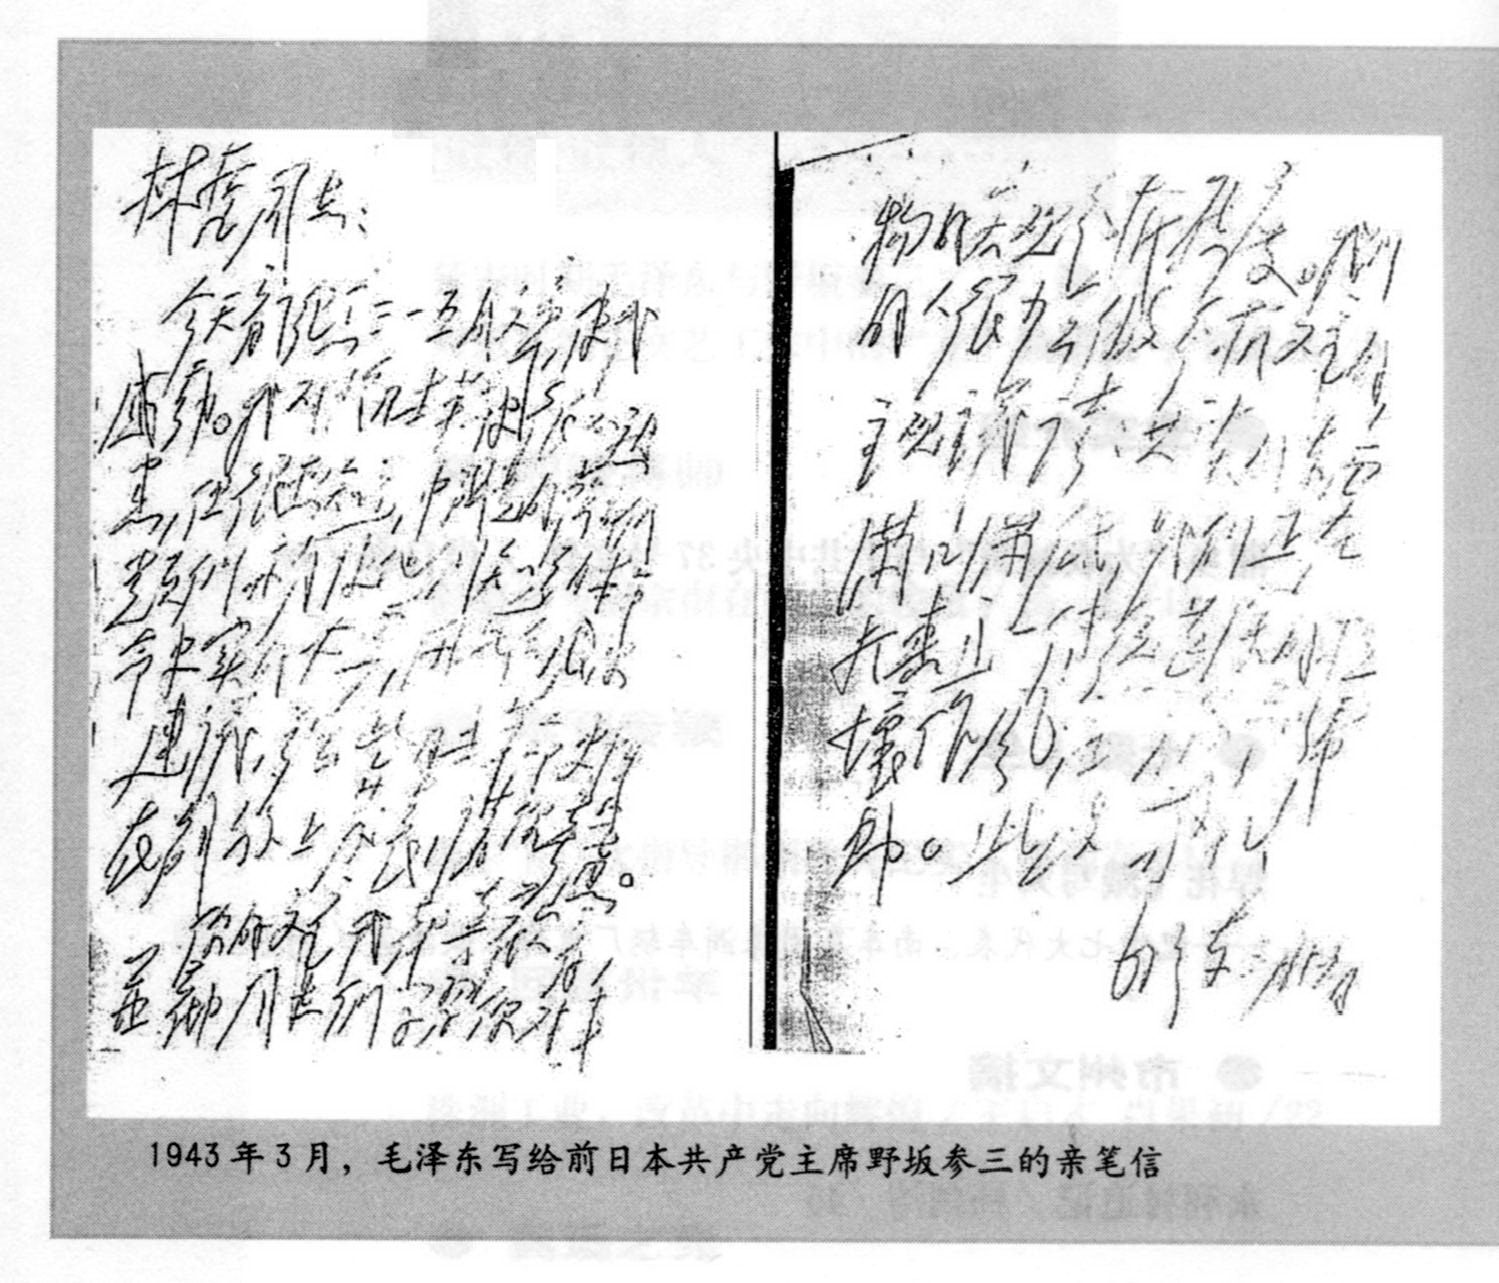
\includegraphics[scale=0.7]{../figure/lz1.jpg} 
\end{center}
   


\newpage


\section*{\myformat{致野坂参三}\\\myformat{(一九四五年五月二十八日)}}
\begin{introduction}\item
二〇〇三年七月,日本一桥大学教授加藤哲郎发现了两封毛泽东致野坂参三的信,本文即为其中之一。现据庆应义塾大学教授寺出道雄与徐一睿文章《毛沢東の野坂参三宛て書簡》(以下简称《书简》)中的简体字本,并参照信件手稿照片整理出本文。
\end{introduction}\\~\\
冈野进\footnote[1]{“冈野进”为野坂参三化名。}同志:\\
  此件看了,觉得很好,使我懂得了日本共产党的具体纲领。关于没收垄断资本(操纵国民生计的东西)一条,确定得很正确,这在英国、法国的共产党都是如此,中国党也是如此,现在日本党又有了。只有美国共产主义者\footnote[2]{此处“者”在《书简》中为“仍”,据手稿照片改。}还没有这条纲领。也许那里的情况是特殊的,他们不提此点乃有他们的理由;但是我颇感怀疑,觉得他们没有找到出路;此点还待研究,希望你提供意见。去年出版的白劳德同志的《德黑兰》一书,你见了没有,希望你看一下,将来我们谈一次。\\
  此外,有几处小的地方,开列于下:\\
  15页,2行,“新兵和老兵比较多”,是否为“新兵较老兵为多”之意,如果是,似宜改一下。\\
  31页,5行,“上下级指挥官”,上下级三字似以去掉为宜。同页9行,“大小政治家”,大小二字似改“反动”二字为宜。同页,10行,“下层法西斯分子”,下层二字似宜去掉。同页,11行,“思想检事等”之下,似宜加上“中的积极分子”等字。这个问题,目前宣传时期,不宜牵涉得太广泛;待将来实行时期,依照群众发动的程度,临时伸缩处理,似较有利。\\
  37页,10行,“尽速由一般人民”,尽速二字似可去掉。这个投票问题,那时究竟以速为有利,或者\footnote[3]{ 此处“者”在《书简》中为“似”,据手稿照片改。}以缓为有利,要看情况才能决定。依我估计,日本人民不要天皇,恐怕不是短期所能做到的。\\
  以上,请加斟酌,并送博古发表,广播。\\
同志的敬礼!

\begin{flushright}
毛泽东\\
五月二十八日
\end{flushright}
\begin{center}
    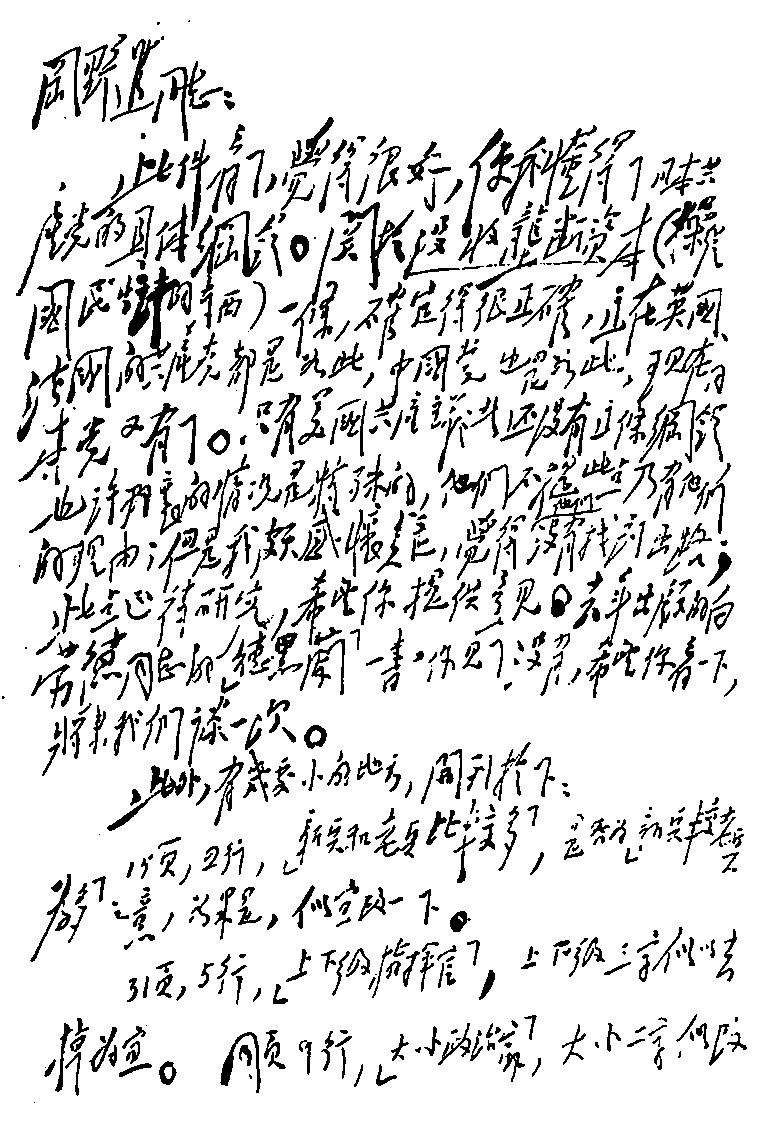
\includegraphics[scale=1.1]{../figure/lz21.jpg}
\end{center}
\begin{center}
    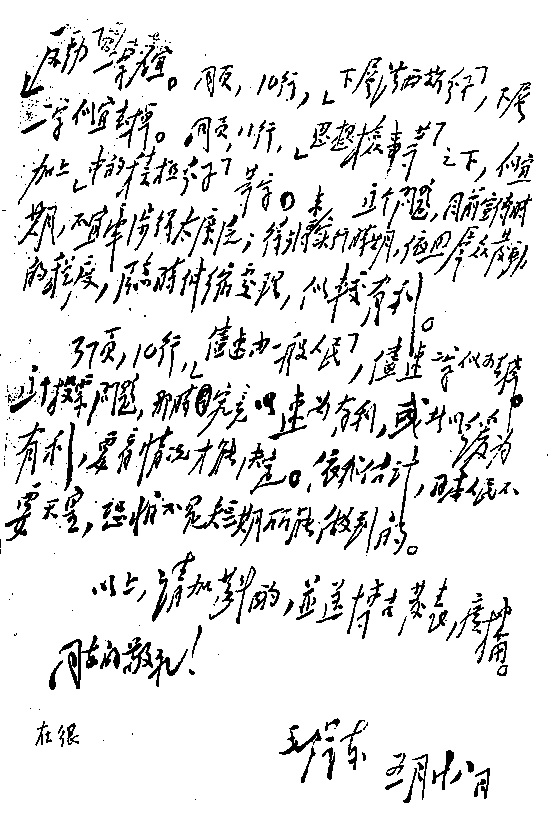
\includegraphics[scale=1.1]{../figure/lz22.jpg}
\end{center}
\newpage

\section*{\myformat{致达赖喇嘛}\\\myformat{(一九五四年四月十日)}}
\begin{introduction}\item
二〇一〇年九月日本横滨国立大学教授村田忠禧在西藏博物馆发现本文手稿,后将手稿照片及日译文发表于《关于在西藏博物馆发现的毛泽东写给达赖喇嘛的信》一文中(《东亚论坛》第七期,二〇一一年十二月)〔村田忠禧:西藏博物館で見つけた毛沢東のダライラマに宛てた書簡について,東アジア論壇,第七号〕。现据手稿照片录入。
\end{introduction}
\\~\\
达赖喇嘛先生:\\
感谢你去年八月一日的来信和礼物。解放后你们在西藏作了不少对国家和西藏民族有益的事,是很好的。正如你的来信所说,为了使西藏僧俗人民对新的祖国更加了解,为了日渐巩固和加强汉藏民族的团结,西藏每年有些人到内地来参观,确实很好。除此以外,西藏还可以选送一些青年到内地来短期或长期地学习,以便更好地培养建设西藏的民族干部。\\
  随函附上牛奶分离机两部,扩音机壹部,两用收音机壹台。顺祝健康。\\

\begin{flushright}
毛泽东\\
一九五四年四月十日
\end{flushright}

\begin{center}
    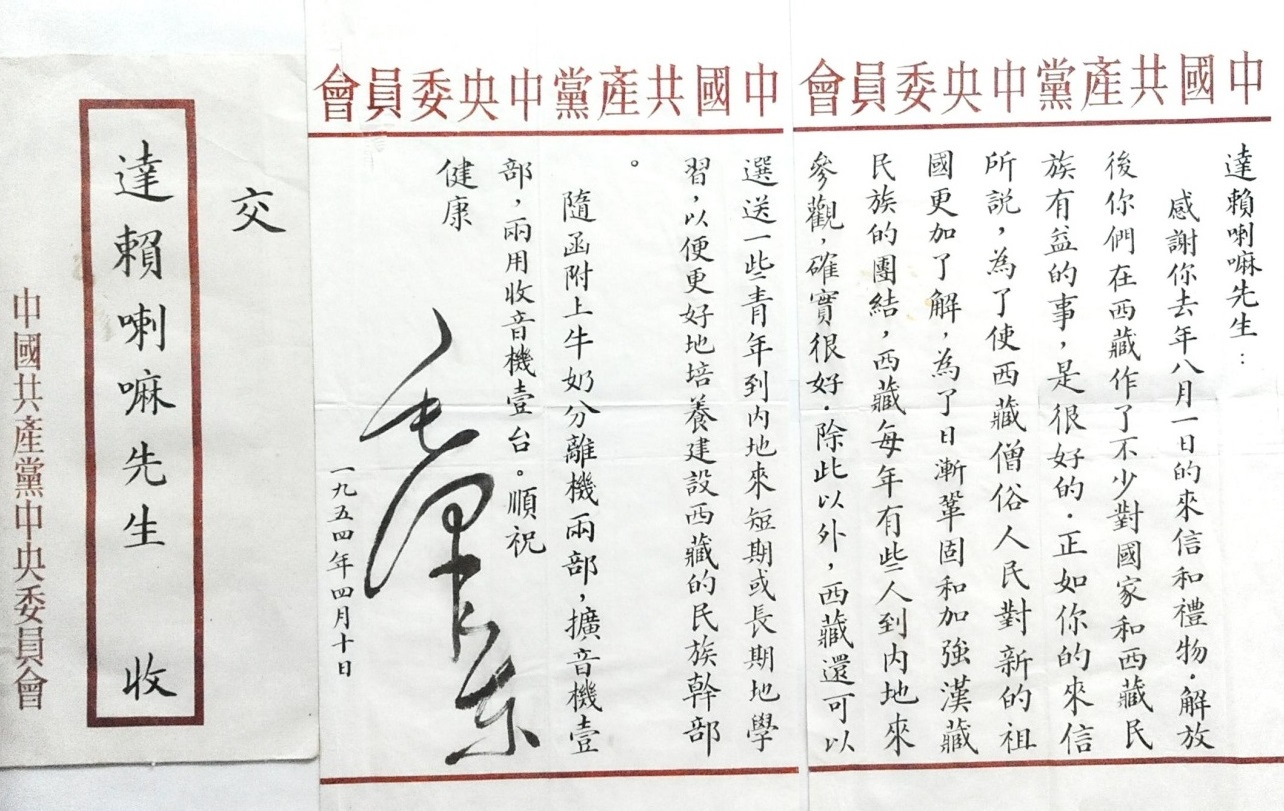
\includegraphics[scale=0.5]{../figure/dllm.jpg}
\end{center}
\end{document}
